\documentclass[8pt]{extarticle}
\usepackage[
  verbose,
  paperwidth=115.4mm,
  paperheight=183.4mm,
  left=9.7mm,
  right=9.7mm,
  top=9.8mm,
  bottom=12.2mm
]{geometry}

\usepackage{fontspec}
\usepackage{ctex}
\usepackage{paratype}
\usepackage{newunicodechar}

\usepackage{amsmath}
\usepackage{amssymb}
\usepackage{amsfonts}
\usepackage{esint}
\usepackage{stmaryrd}

\usepackage[mathbf=sym]{unicode-math}
\setmainfont{STIX Two Text}
\setmathfont{STIX Two Math}
\newunicodechar{∈}{\ensuremath{\in}}
\newunicodechar{≤}{\ensuremath{\leq}}
\newunicodechar{≥}{\ensuremath{\geq}}
\newunicodechar{≠}{\ensuremath{\neq}}
\newunicodechar{⊂}{\ensuremath{\subset}}
\newunicodechar{∅}{\ensuremath{\varnothing}}
\newunicodechar{∩}{\ensuremath{\cap}}
\newunicodechar{→}{\ensuremath{\rightarrow}}
\newunicodechar{€}{\ensuremath{\in}}

\setsansfont{Arial}
\setmonofont{Courier New}

\usepackage{makecell}
\usepackage{wasysym}
\usepackage{pifont}
\usepackage[export]{adjustbox}
\usepackage{graphicx}
\usepackage{mdframed}
\usepackage{booktabs,array,multirow}
\usepackage{tabularx}
\usepackage{hyperref}
\hypersetup{colorlinks=true, linkcolor=blue, filecolor=magenta, urlcolor=cyan,}
\urlstyle{same}
\usepackage[most]{tcolorbox}
\definecolor{mygray}{RGB}{240,240,240}
\tcbset{
  colback=mygray,
  boxrule=0pt,
}
\graphicspath{ {./images/} }
\newcommand{\HRule}{\begin{center}\rule{0.9\linewidth}{0.2mm}\end{center}}
\newcommand{\customfootnote}[1]{
  \let\thefootnote\relax\footnotetext{#1}
}
\newcommand{\lt}{\mathrel{<}}
\newcommand{\gt}{\mathrel{>}}
\newcommand*\circled[1]{\tikz[baseline=(char.base)]{\node[shape=circle,draw,inner sep=1.5pt] (char) {\small #1};}}
\setcounter{MaxMatrixCols}{256}
\begin{document}
B.M.Благодатских

\section*{BBEAEHME BONTIMMAJIBHOE YMPABJIEHME}

\begin{itemize}\relax
\item\relax линейная теория -
\end{itemize}

Допущено Министерством образования Российской Федерации в качестве учебника для студентов высших учебных заведений

\begin{center}

\includegraphics[max width=0.2\textwidth]{images/bo_d547okref24c73bgfch0_0_438_2057_159_161_0.jpg}
\end{center}
\hspace*{3em} 

Peцензенты:

кафедра высшей математики МФТИ (заведующий кафедрой - д-p физ.- мат. наук, чл.-корр. РАО, проф. Г.Н. Яковлев) и д-р физ.-мат. наук, проф.

M.C. Никольский

Благодатских В.И.

Б 68 Введение в оптимальное управление (линейная теория): Учебник/В.И. Благодатских. Под ред. В.А. Садовничего. – M.: Bысш. шк., 2001. - 239 c.: ил.

\section*{ISBN 5-06-003983-8}

Книга состоит из 12 лекций, в которых изложен необходимый математи- ческий аппарат (элементы выпуклого анализа, теория опорных функций, све- дения из теории многозначных отображений) и подробно рассмотреиа ли- нейная задача быстродействия. В дополнениях приведены доказательства наиболее технически сложных результатов.

Для студентов высших учебных заведений, а также аспирантов и науч- ных работников, использующих в своей деятельности математическую тео- рию оптимального управления.

УДК 510

ББК 22.1

 \textcopyright  ГУП «Издательство «Высшая школа», 2001

Оригинал-макет данного издания является собственностью издательства «Высшая школа», и его репродуцирование (воспроизведение) любым способом без согласия изда- тельства запрещается.

\begin{center}

\includegraphics[max width=0.6\textwidth]{images/bo_d547okref24c73bgfch0_2_387_15_686_1059_0.jpg}
\end{center}
\hspace*{3em} 

\section*{OB ABTOPE}

Виктор Иванович Благодатских родился 18 мая 1946 г. в уд- муртском селе Сюмси в большой семье, где было девять детей. В школьные годы он был очень увлекающимся мальчишкой: занимался во всех школьных кружках, и без него не проходила, пожалуй, ни одна республиканская олимпиада по математике, химии, физике. И практически всегда он становился победите- лем. Именно таким образом в 1963 г. он попал в Колмогоровскую летнюю математическую школу под Москвой. Это и решило его дальнейшую судьбу. После окончания средней школы он поступил на механико-математический факультет Московского государственного университета.

Студенческие годы были для него поистине счастливыми. Кипучая энергия и огромный интерес к жизни позволили ему сочетать учебу в лучшем вузе страны с такими увлекательными спортивными занятиями, как альпинизм, спелеология, туризм, прыжки с парашютом, прыжки в воду. В дни юности он приоб- рел свое самое главное богатство — множество друзей. Он легко сходился с людьми, любил их, поэтому рядом с ним всем было тепло и хорошо. Свою любовь и судьбу он нашел тогда же в секции спелеологии.

После окончания МГУ ему посчастливилось попасть в круг учеников замечательного математика и человека академика Льва Семеновича Понтрягина. В это время Виктор Иванович серьезно начал заниматься математической теорией оптималь- ного управления, что стало делом всей его жизни. Он закончил аспирантуру Математического института им. В.А. Стеклова (MИАН) и работал там до конца жизни. Его кандидатская и докторская диссертации посвящены развитию теории оптималь- ного управления с применением аппарата дифференциальных включений. Эти работы хорошо известны в мировом математи- ческом сообществе.

Много лет Виктор Иванович был помощником Л.С. Понтря- гина в его многогранной научной деятельности. С самого осно- вания в 1973 г. факультета вычислительной математики и ки- бернетики МГУ под руководством Л.С. Понтрягина создавалась кафедра оптимального управления, и Виктор Иванович внес ог- ромный вклад в организацию учебного процесса. Он разработал и много лет читал курс лекций "Оптимальное управление", ко- торый пользовался большим успехом у студентов факультета.

Написанные им ранее на основе этих лекций учебные по- собия "Линейная теория оптимального управления" (М.: Изд- во МГУ, 1978) и "Теория дифференциальных включений" Ч. 1 (М.: Изд-во МГУ, 1979) сыграли важную роль в формировании взглядов на предмет многих специалистов московской школы оптимального управления. Вообще, Виктор Иванович был заме- чательным учителем. Среди его учеников несколько докторов физико-математических наук и много кандидатов. Свой курс лекций он передал ученикам. И сегодня этот курс живет и разви- вается на основе подхода, который заложил В.И. Благодатских.

Предлагаемая читателю книга “Введение в оптимальное управление" является своего рода итогом многолетней педа- гогической работы профессора В.И. Благодатских. Она была задумана автором как введение в предмет, охватывающее все основные результаты теории как в линейном, так и в нелиней- ном случаях. Предполагалось, что изложенный материал будет рассчитан на два семестра лекций.

5 августа 1998 г. на пятьдесят третьем году жизни Виктор Иванович скоропостижно скончался, не осуществив до конца своего замысла. Он успел написать только первую, посвящен- ную линейной теории, часть книги.

Рукопись подготовили к изданию коллеги Виктора Ивано- вича по кафедре. Основная роль в подготовке рукописи принад- лежит его ученику, д-ру физ.-мат. наук, проф. Сергею Миро- новичу Асееву, который дополнил материал книги параграфом "Условие общности положения" (см. лекцию 12).

П.В. Благодатских

\section*{ЛЕКЦИЯ 1}

\begin{itemize}\relax
\item\relax Общая постановка задачи оптимального управле- ния: динамика объекта, класс допустимых управле- ний, начальное и конечное состояния объекта, кри- терий качества.
\end{itemize}

\begin{itemize}\relax
\item\relax Основные вопросы математической теории опти- мального управления: управляемость, существова- ние оптимального управления, необходимые условия оптимальности, достаточные условия оптималь- ности, единственность оптимального управления.
\end{itemize}

\begin{itemize}\relax
\item\relax Постановка линейной задачи быстродействия.
\end{itemize}

\section*{1.1. Общая постановка задачи оптимального управления}

Динамика объекта. Для задачи оптимального управле- ния характерно наличие некоторого динамического объекта, т.е. объекта, меняющегося во времени. Пусть положение объекта в каждый момент времени и полностью характеризуется набором параметров \({x}^{1}\left( t\right) ,\ldots ,{x}^{n}\left( t\right)\) . Это могут быть координаты объек- та в какой-то системе координат, координаты скорости и т.п. Вектор

\[
\mathbf{x}\left( t\right)  = \left( {{x}^{1}\left( t\right) ,\ldots ,{x}^{n}\left( t\right) }\right)
\]

называется фазовым вектором объекта. Предполагается, что движением объекта можно управлять, т.е. объект снабжен не- которыми рулями, от положения которых зависит его поведе- ние. Пусть положение рулёй характеризуется в каждый момент времени t набором параметров \({u}^{1}\left( t\right) ,\ldots ,{u}^{m}\left( t\right)\) . Вектор

\[
u\left( t\right)  = \left( {{u}^{1}\left( t\right) ,\ldots ,{u}^{m}\left( t\right) }\right)
\]

называется управляющим параметром объекта или управлени- ем. Естественно предположить, что состояние объекта в данный момент времени t зависит от того, какие значения принимает управление \(\mathbf{u}\left( t\right)\) до момента времени t, и не зависит от будущего поведения управления.

В зависимости от того, как выражается зависимость векто- ра фазового состояния \(x\left( t\right)\) or управления \(u\left( t\right)\) , paccматривают различные динамические объекты. Например, эта зависимость может описываться системой дифференцальных уравнений

\[
\dot{\mathbf{x}} = \mathbf{f}\left( {t,\mathbf{x},\mathbf{u}}\right) . \tag{1.1}
\]

В этом случае, зная значение управления \(\mathbf{u}\left( t\right)\) в каждый момент времени t, можно определить mpaeкторию объекта х(t) как ре- шение дифференциального уравнения

\[
\dot{\mathbf{x}} = \mathbf{f}\left( {t,\mathbf{x},\mathbf{u}\left( t\right) }\right) .
\]

Будем считать, что каким-то образом задана динамика объ- екта, т.е. закон изменения вектора состояния \(\mathbf{x}\left( t\right)\) в зависимос- ти от изменения вектора управления и(t).

Kласс допустимых управлений. Ясно, что в конкретных физических объектах управление и(t) может не быть произволь- ным. На него наложены какие-то ограничения, вытекающие из физического смысла управления. Например, если и'(t) — тяга двигателя, то в каждый момент времени она должна удовлетво- рять ограничению

\[
{u}_{\min } \leq  {u}^{1}\left( t\right)  \leq  {u}_{\max }
\]

При этом тяга и \({u}^{1}\left( t\right)\) может принимать также и крайние значе- ния и \({u}_{\min }\) и \({u}_{\max }\) . Обычно предполагают, что вектор управления \(\mathbf{u}\left( t\right)\) удовлетворяет в каждый момент времени t ограничению

\[
\mathbf{u}\left( t\right)  \in  U \tag{1.2}
\]

где U — некоторое заданное множество. Как правило, в кон- кретных физических объектах множество U замкнуто. Эта за- мкнутость и не позволяет в общем случае исследовать поведение управляемого объекта методами классического вариационного исчисления. Кроме ограничения вида (1.2) могут быть наложе- ны ограничения на зависимость управления и(t) от времени. Например, из физического смысла допустимыми управлениями могут быть либо гладкие функции, либо непрерывные, либо ку- сочно непрерывные и т.п. Будем считать, что каким-то образом задан класс допустимых управлений и \(\left( t\right)\) .

Начальное и конечное состояния объекта. Предполо- жим, что задан начальный момент времени \({t}_{0}\) и множество \({M}_{0}\) допустимых начальных состояний объекта. Кроме того, жела- тельно управлять объектом так, чтобы в какой-то конечный момент времени \({t}_{1}\) объект перешел на некоторое множество \({M}_{1}\) допустимых конечных состояний. Будем считать, что допусти- мое управление \(\mathbf{u}\left( t\right)\) переводит объект из множества начальных состояний \({M}_{0}\) на множество конечных состояний \({M}_{1}\) на отрезке времени \(\left\lbrack  {{t}_{0},{t}_{1}}\right\rbrack\) , если соответствующее этому управлению фазовое состояние объекта \(\mathbf{x}\left( t\right)\) удовлетворяет условиям

\[
\mathbf{x}\left( {t}_{0}\right)  \in  {M}_{0},\;\mathbf{x}\left( {t}_{1}\right)  \in  {M}_{1}. \tag{1.3}
\]

Заметим, что конечный момент времени \({t}_{1}\) может быть, во- обще говоря, не фиксированным, а определяться из условия по- падания вектора \(\mathbf{x}\left( t\right)\) на конечное множество \({M}_{1}\) . Итак, предпо- ложим, что допустимые множества \({M}_{0}\) и \({M}_{1}\) заданы.

Критерий качества. Может случиться, что управляемый объект можно перевести из множества \({M}_{0}\) на множество \({M}_{1}\) многими способами. Часто на практике желательно среди всех таких переходов выбрать в каком-то смысле наилучший. Обыч- но предполагается, что каждому допустимому управлению \(\mathbf{u}\left( t\right)\) , заданному на отрезке \(\left\lbrack  {{t}_{0},{t}_{1}}\right\rbrack\) , и соответствующей ему траекто- рии объекта \(\mathbf{x}\left( t\right)\) сопоставлено некоторое число \(J\) , оценивающее качество пары \(\mathbf{u}\left( t\right) ,\mathbf{x}\left( t\right)\) , т.е. задан функционал, или крите- рий, качества \(J\left( {\mathbf{u}\left( t\right) ,\mathbf{x}\left( t\right) }\right)\) . Например, этот функционал может иметь вид

\[
J\left( {\mathbf{u}\left( t\right) ,\mathbf{x}\left( t\right) }\right)  = {\int }_{{t}_{0}}^{{t}_{1}}{f}^{0}\left( {s,\mathbf{x}\left( s\right) ,\mathbf{u}\left( s\right) }\right) {ds}. \tag{1.4}
\]

Теперь можно сформулировать задачу оптимального управ- ления. Эта задача заключается в нахождении таких допустимо- го управления \({\mathbf{u}}^{ * }\left( t\right)\) и соответствующей ему траектории объек- та \({\mathbf{x}}^{ * }\left( t\right)\) , переводящей объект из множества начальных состо- яний \({M}_{0}\) на множество конечных состояний \({M}_{1}\) , что при этом функционал качества \(J\left( {\mathbf{u}\left( t\right) ,\mathbf{x}\left( t\right) }\right)\) принимает минимальное зна- чение, т.е.

\[
J\left( {{\mathbf{u}}^{ * }\left( t\right) ,{\mathbf{x}}^{ * }\left( t\right) }\right)  = \min J\left( {\mathbf{u}\left( t\right) ,\mathbf{x}\left( t\right) }\right) .
\]

Здесь минимум берется по всевозможным допустимым управле- ниям \(\mathbf{u}\left( t\right)\) и соответствующим траекториям \(\mathbf{x}\left( t\right)\) , переводящим объект из множества начальных состояний \({M}_{0}\) на множество конечных состояний \({M}_{1}\) .

Рассмотрим примеры задач оптимального управления.

Пример 1. Пусть космический корабль движется по неко- торой круговой орбите вокруг Земли. С разумной степенью точ- ности поведение корабля можно описать системой дифференци- альных уравнений типа (1.1). При этом координатами вектора фазового состояния х(t) могут быть координаты вектора поло- жения корабля относительно неподвижной системы координат, связанной с Землей, координаты вектора скорости, углы, зада- ющие ориентацию корабля, угловая скорость и т.п. Координа- тами вектора управления \(\mathbf{u}\left( t\right)\) могут быть углы поворота струи реактивного двигателя, расход топлива в единицу времени и т.п. Выбирая те или иные значения координат вектора управ- ления \(\mathbf{u}\left( t\right)\) ,можно заставить космический корабль двигаться по той или иной траектории \(\mathbf{x}\left( t\right)\) .

Предположим, что корабль нужно перевести на новую кру- говую орбиту, т.е. подобрать управление и(t) таким образом, чтобы соответствующая траектория \(\mathbf{x}\left( t\right)\) начиналась в момент времени б на первой круговой орбите и заканчивалась в неко- торый момент времени \({t}_{1}\) на второй круговой орбите. При этом за множество начальных состояний \({M}_{0}\) можно взять значения координат корабля на первой орбите, допустимые начальные скорости и т.п., т.е. значения вектора х(би). Аналогично обстоит дело с множеством конечных состояний \({M}_{1}\) .

Критерием качества может служить общее количество топ- лива, затраченное на переход с первой орбиты на вторую. Таким образом, задача оптимального управления будет заключаться в выборе таких допустимого управления и(t) и соответствующей траектории \(\mathbf{x}\left( t\right)\) ,чтобы перевод космического корабля с первой круговой орбиты на вторую осуществлялся с минимальным рас- ходом топлива.

Пример 2. Рассмотрим физический маятник, который на- ходится в положении равновесия. Если у — отклонение маятни- ка от положения равновесия, то уравнение маятника в случае колебаний с малой амплитудой имеет вид

\[
\ddot{y} + y = 0.
\]

Предположим, что к маятнику можно прикладывать внешнюю управляющую силу и, ограниченную по величине, например единицей, так что |u| ≤1. Тогда уравнение управляемого маят- ника имеет вид

\[
\ddot{y} + y = u.
\]

Приведем это уравнение к виду (1.1), положив х1 = y, x2 = j. Тогда имеем

\[
\left\{  \begin{array}{l} {\dot{x}}^{1} = {x}^{2}, \\  {\dot{x}}^{2} =  - {x}^{1} + u. \end{array}\right. \tag{1.5}
\]

В данном случае фазовый вектор \(x = \left( {{x}^{1},{x}^{2}}\right)\) имеет всего две координаты: \({x}^{1} = y\) — отклонение маятника от положения рав- новесия и \({x}^{2} = \dot{y}\) — скорость отклонения. Положение равновесия при выключенном управлении, т.е. при и = 0, задается условием \({x}^{1} = 0,{x}^{2} = 0\) . Предположим, что под воздействием каких-либо внешних возмущений маятник отбрасывается в произвольное положение \({\mathbf{x}}_{0} = \left( {{\mathbf{x}}_{0}^{1},{\mathbf{x}}_{0}^{2}}\right)\) . Haxoxдение в этом положении нежела- тельно из физических соображений, и нужно как можно скорее перевести маятник в положение равновесия, выбирая для этого соответствующим образом внешнюю силу и(t), при этом опять же из физических соображений функция \(u\left( t\right)\) должна быть, на- пример, кусочно непрерывной.

Таким образом, приходим к следующей задаче оптимального управления. Подобрать такую кусочно непрерывную внешнюю силу и(t), удовлетворяющую ограничению |u| ≤ 1, чтобы соот- ветствующая траектория маятника х(t), т.е. решение уравнения (1.5), nepeшла из начального состояния \({M}_{0} = \left\{  {\mathbf{x}}_{0}\right\}   = \left\{  \left( {{\mathbf{x}}_{0}^{1},{\mathbf{x}}_{0}^{2}}\right) \right\}\) в положение равновесия \({M}_{1} = \{ \left( {\mathbf{0},\mathbf{0}}\right) \}\) за наименьшее время.

\section*{1.2. Основные вопросы математической теории оптимального управления}

Выше мы определили основные элементы постановки задачи оптимального управления и разобрали два примера. Прежде чем перейти к математическому исследованию задачи оптимального управления, рассмотрим, какие вопросы включает в себя мате- матическая теория оптимального управления.

Управляемость. Прежде всего возникает вопрос, а существу- ет ли хотя бы одно допустимое управление \(\mathbf{u}\left( t\right)\) , которое пере- водит динамический объект из множества начальных состояний \({M}_{0}\) на множество конечных состояний \({M}_{1}\) , т.е. существует ли такое допустимое управление \(\mathbf{u}\left( t\right)\) , при котором соответству- ющий вектор фазового состояния \(\mathbf{x}\left( t\right)\) удовлетворяет условиям (1.3). Если этот вопрос решается положительно, то будем гово- рить, что объект является управляемым из множества \({M}_{0}\) на множество \({M}_{1}\) . В противном случае сама постановка задачи оптимального управления теряет смысл.

Существование оптимального управления. Если во- прос об управляемости решается положительно, т.е. существует некоторое управление \(\mathbf{u}\left( t\right)\) , переводящее объект из множества \({M}_{0}\) на множество \({M}_{1}\) , то необходимо выяснить, существует ли оптимальное управление. Инженеры, как правило, при решении конкретных задач не ставят такого вопроса, а просто пытают- ся найти наилучшее управление доступными им средствами. С математической точки зрения этот вопрос является одним из основных, и если оптимального управления не существует, то дальнейшие поиски его становятся бессмысленными. В матема- тике мы имеем дело всегда лишь с некоторой моделью реаль- ного физического объекта, и отсутствие в модели оптимального управления может указывать на то, что модель построена не- правильно.

Необходимые условия оптимальности. Если оптималь- ное управление в задаче существует, то далее нужно развивать методы нахождения этого оптимального управления. Даже в простых задачах может оказаться бесконечно много допусти- мых управлений, переводящих объект из множества начальных состояний \({M}_{0}\) на множество конечных состояний М1. Поэтому простым перебором всех допустимых управлений обойтись не удается. Возникает вопрос, как сузить класс управлений, по- дозрительных на оптимальность. Решить его позволяют необ- ходимые условия оптимальности. Таким образом, оптималь- ное управление нужно искать лишь среди множества допусти- мых управлений, удовлетворяющих необходимым условиям оп- тимальности.

Таким необходимым условием оптимальности является принцип максимума Понтрягина. Первоначально он был вы- сказан в качестве гипотезы академиком Львом Семеновичем Понтрягиным в 1953 г. для управляемых систем, динамика которых описывается уравнением вида (1.1), а затем доказан его учениками. По существу, с принципа максимума и началась математическая теория оптимального управления. В некоторых задачах оказывается даже, что принципу максимума удовлетво- ряет лишь конечное число управлений, среди которых уже не- трудно выбрать оптимальное. Полное доказательство принципа максимума было опубликовано в 1961 г. Л.С. Понтрягиным и его учениками в книге [1]. Применение принципа максимума сразу же позволило решить многие интересные инженерные задачи, а в других задачах существенно приблизиться к нахождению оптимального управления. Не случайно уже в 1962 г. эта книга была отмечена Ленинской премией.

Достаточные условия оптимальности. Во многих зада- чах, несмотря на то, что необходимые условия оптимальности и позволяют сузить класс управлений, подозрительных на оп- тимальность, все же этот класс остается достаточно широким. Отобрать действительно оптимальное управление в этом классе позволяют достаточные условия оптимальности. Если некото- poe управление \(u\left( t\right)\) из этого класса удовлетворяет достаточ- ным условиям оптимальности, то тем самым гарантируется его оптимальность. Конечно, может случиться, что достаточным условиям оптимальности удовлетворяет не одно, а несколько управлений. Тем самым гарантируется, что все они оптималь- ны, т.е. функционал качества принимает на всех этих управле- ниях одинаковое и притом минимальное значение.

Единственность оптимального управления. Инжене- рам очень важно знать, является ли оптимальное управление единственным. Если оно единственно, то в конкретных управля- емых объектах реализация единственного оптимального управ- ления может оказаться существенно проще. Поэтому вопрос о единственности оптимального управления также входит в чис- ло основных вопросов математической теории оптимального управления.

Конечно, мы перечислили не все вопросы, которые могут возникнуть при решении задачи оптимального управления, а только основные. Естественно, что эти вопросы могут исследо- ваться для конкретного управляемого объекта не обязательно в той последовательности, в какой они здесь приведены. На- пример, если сначала установлено, что оптимальное управление существует, и мы нашли единственное допустимое управление \(\mathbf{u}\left( t\right)\) , переводящее объект из множества начальных состояний \({M}_{0}\) на множество конечных состояний \({M}_{1}\) и удовлетворяющее необходимым условиям оптимальности, то тем самым гаранти- руется, что это управление и(t) оптимально.

Линейная задача быстродействия. Итак, мы сформули- ровали общую постановку задачи оптимального управления и рассмотрели некоторые основные вопросы, возникающие при решении этой задачи. В настоящей книге мы в основном бу- дем изучать математическую теорию для простейшей задачи оптимального управления — линейной задачи быстродействия. Динамика объекта в этой задаче будет описываться системой линейных дифференциальных уравнений

\[
\dot{\mathbf{x}} = A\mathbf{x} + \mathbf{u}, \tag{1.6}
\]

где х — п-мерный вектор фазового состояния объекта, и — \(n\) -мерный вектор управления, на который наложено ограниче- ние \(u\left( t\right)  \in  U,A -\) постоянная матрица размером \(n \times  n\) . Зная некоторую допустимую функцию управления и(t) и начальное состояние объекта \(\mathbf{x}\left( {t}_{0}\right)  = {\mathbf{x}}_{0}\) ,можно получить единственную функцию \(\mathbf{x}\left( t\right)\) вектора фазового состояния объекта как решение дифференциального уравнения (1.6). Класс допустимых управ- лений определим позднее, когда будет изучен некоторый вспо- могательный математический аппарат.

Начальное и конечное состояния объекта будем выбирать как элементы некоторых непустых и компактных подмножеств \({M}_{0}\) и \({M}_{1}\) соответственно из n-мерного фазового пространства. Критерием качества будет служить время перехода из множес- тва \({M}_{0}\) на множество \({M}_{1}\) ,т. e.

\[
J\left( {\mathbf{u}\left( t\right) ,\mathbf{x}\left( t\right) }\right)  = {t}_{1} - {t}_{0}.
\]

Такой критерий качества получается из критерия качества (1.4), когда подынтегральная функция имеет вид

\[
{f}^{0}\left( {t,\mathbf{x}\left( t\right) ,\mathbf{u}\left( t\right) }\right)  \equiv  1
\]

Таким образом, мы пришли к постановке линейной задачи быстродействия. Эта задача заключается в нахождении допус- тимого управления и*(t) и соответствующего ему решения х*(t) уравнения (1.6), переводящего объект из множества начальных состояний \({M}_{0}\) на множество конечных состояний \({M}_{1}\) за мини- мальное время. Приведенный выше пример 2 является линейной задачей быстродействия.

Линейная задача быстродействия выбрана для первого зна- комства с теорией оптимального управления не случайно. Она обладает многими преимуществами.

Во-первых, для линейного дифференциального уравнения (1.6) можно в явном виде получить зависимость траектории х(t) от управления и(t). Это позволяет эффективно исследовать все основные вопросы математической теории оптимального управ- ления.

Во-вторых, на примере линейной задачи быстродействия до- статочно ярко проявляются все характерные трудности, прису- щие общим задачам оптимального управления.

Первая часть книги (лекции 2 — 5) посвящена изучению вспомогательного математического аппарата. Подробно будут рассмотрены такие понятия, как опорная функция, многознач- ные отображения, интегралы от многозначных отображений и т.д. Эти понятия находят широкое применение в различных разделах математики. С их помощью во второй части книги будут исследованы основные вопросы математической теории оптимального управления на примере линейной задачи быстро- действия.

\section*{JIEKIJIN 2}

\begin{itemize}\relax
\item\relax Основные определения и обозначения.
\end{itemize}

\begin{itemize}\relax
\item\relax Пространство \(\Omega \left( {E}^{n}\right)\) , cocmoящее из всех непустых компактных подмножеств евклидова векторного пространства \({E}^{n}\) .
\end{itemize}

\begin{itemize}\relax
\item\relax Onepaquu сложения двух элементов и умножение элемента на число в пространстве Ω(Ег).
\end{itemize}

\begin{itemize}\relax
\item\relax Образ множества при линейном преобразовании.
\end{itemize}

\begin{itemize}\relax
\item\relax Понятие расстояния в пространстве Ω(Ег).
\end{itemize}

\section*{2.1. Основные определения}

Пространство \({E}^{n}\) . Рассмотрим n-мерное евклидово век- торное пространство \({E}^{n}\) c элементами x = \(\left( {{x}^{1},\ldots ,{x}^{n}}\right)\) . B част- ности, \({E}^{1}\) — числовая ось, \({E}^{2}\) — двумерная плоскость и т.д. Как правило, строчными буквами (жирным шрифтом) будем обозначать векторы или, что то же самое, точки пространст- ва \({E}^{n}\) , a прописными — подмножества пространства Е". При этом векторы будем иногда рассматривать как множества, со- стоящие из одной точки. В этом случае они будут записаны в фигурных скобках. Например, х — точка, а \{x\} — множество, состоящее из одной точки х. Пространство Е" является линей- ным пространством с обычными операциями сложения векто- ров, умножения вектора на число и скалярным произведением \(\langle \mathbf{x},\mathbf{y}\rangle  = {x}^{1}{y}^{1} + \cdots  + {x}^{n}{y}^{n}\) . Это пространство является также нормированным с нормой \(\parallel \mathbf{x}\parallel  = \sqrt{\langle \mathbf{x},\mathbf{x}\rangle }\) . Будем использовать только такую норму в пространстве E". Эта норма естествен- ным образом определяет расстояние \(\rho \left( {\mathbf{x},\mathbf{y}}\right)  = \parallel \mathbf{x} - \mathbf{y}\parallel\) между точками \(\mathbf{x},\mathbf{y} \in  {E}^{n}\) ,или метрику в пространстве E".

Множества. Рассмотрим различные виды множеств в про- странстве \({E}^{n}\) . При этом для множеств будем использовать обычные символы включения C, равенства =, неравенства ≠, объединения U, пересечения ∩ и дополнения  \textbackslash  одного множества до другого. Символом ∅ будем обозначать пустое множество.

Точка \(\mathbf{x} \in  {E}^{n}\) называется предельной точкой множества \(F\) , если в любой ее окрестности содержится хотя бы одна точка множества \(F\) . Множество \(F\) называется замкнутым, если оно содержит все свои предельные точки. Замыканием \(\bar{F}\) множества \(F\) называется наименьшее замкнутое множество, содержащее множество \(F\) . Ясно, что если множество \(F\) замкнуто, то \(\bar{F} = F\) .

Пример 1. Рассмотрим в пространстве E" множество P, заданное условием

\[
P = \left\{  {\mathbf{x} \in  {E}^{n} : \parallel \mathbf{x}\parallel  < 1}\right\}  .
\]

Это множество не является замкнутым, так как, например, пре- дельная точка \(\mathbf{p} = (1,0,\ldots,0)\) множества \(P\) ему не принадле- жит. Ясно, что шар \({S}_{r}\left( \mathbf{a}\right)\) радиуса \(r\) с центром в точке \(\mathbf{a}\) из пространства \({E}^{n}\)

\[
{S}_{r}\left( \mathbf{a}\right)  = \left\{  {\mathbf{x} \in  {E}^{n} : \parallel \mathbf{x} - \mathbf{a}\parallel  \leq  r}\right\} \tag{2.1}
\]

является множеством замкнутым. Шар \({S}_{1}\left( 0\right)\) является замыка- нием множества \(P\) , т.е. \(\bar{P} = {S}_{1}\left( 0\right)\) .

Множество \(F \subset  {E}^{n}\) называется ограниченным, если оно со- держится в шаре некоторого конечного радиуса, т.е. если F ⊂ \(\subset  {S}_{r}\left( 0\right)\) для некоторого \(r \geq  0\) . Множество \(F \subset  {E}^{n}\) называется компактным, если оно замкнуто и ограничено. Так, множество \({S}_{r}\left( \mathbf{a}\right)\) из примера 1 компактно, а множество P некомпактно, так как оно не замкнуто. Прямая линия на плоскости есть множес- тво, некомпактное из-за своей неограниченности.

Если множество F компактно, то модулем |F| множества F назовем число

\[
\left| F\right|  = \mathop{\max }\limits_{{f \in  F}}\parallel f\parallel . \tag{2.2}
\]

В силу компактности множества F и непрерывности нормы || \(f\) || максимум в формуле (2.2) достигается всегда. Геометрический смысл модуля множества F таков: это есть радиус наименьшего шара с центром в начале координат, содержащего множество F (рис. 1), что следует из соотношения

\[
\left| F\right|  = \mathop{\max }\limits_{{f \in  F}}\parallel \mathbf{f}\parallel  = \min \{ r \geq  0 : \parallel \mathbf{f}\parallel  \leq  r,\mathbf{f} \in  F\}  =
\]

\[
= \min \left\{  {r \geq  0 : F \subset  {S}_{r}\left( \mathbf{0}\right) }\right\}  .
\]

\begin{center}
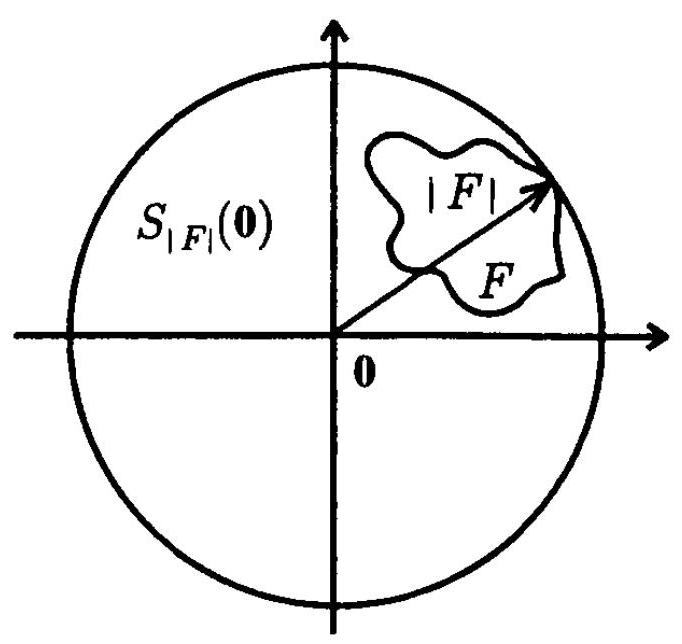
\includegraphics[max width=0.6\textwidth]{images/bo_d547okref24c73bgfch0_16_766_16_682_644_0.jpg}
\end{center}
\hspace*{3em} 

Рис. 1

Таким образом, всегда вы- полняется включение

\[
F \subset  {S}_{\left| F\right| }\left( 0\right) \text{ . } \tag{2.3}
\]

Toчka \(f\) называется внут- ренней точкой множества F, если \({S}_{\varepsilon }\left( f\right)  \subset  F\) для некоторо- ro \(\varepsilon  > 0\) . Множество F назы- вается открытым, если любая его точка внутренняя. Сово- купность всех внутренних то- чек множества \(F\) называется ero внутренностью и обозна- чается через int \(F\) . Tak, в при- мере 1 int \({S}_{1}\left( 0\right)  = P\) . Границей д \(F\) множества \(F\) называется множество \(\partial F = \bar{F} \smallsetminus  \operatorname{int}F\) . Если

\[
S = \left\{  {\mathbf{x} \in  {E}^{n} : \parallel \mathbf{x}\parallel  = 1}\right\}
\]

— единичная сфера в пространстве E", то дP = S.

Множество \(F\) называется выпуклым, если для любых двух точек \({x}_{1}\) и \({x}_{2}\) множества \(F\) отрезок, coединяющий точки \({x}_{1}\) и \({x}_{2}\) ,также принадлежит множеству \(F\) . Oтрезок \(\left\lbrack  {{x}_{1},{x}_{2}}\right\rbrack\) , coehu- няющий две точки \({x}_{1},{x}_{2} \in  {E}^{n}\) ,имеет вид

\[
\left\lbrack  {{\mathbf{x}}_{1},{\mathbf{x}}_{2}}\right\rbrack   = \left\{  {\mathbf{x} = \lambda {\mathbf{x}}_{1} + \left( {1 - \lambda }\right) {\mathbf{x}}_{2} : 0 \leq  \lambda  \leq  1}\right\}  .
\]

Таким образом, множество F называется выпуклым, если для любых точек \({x}_{1},{x}_{2} \in  {E}^{n}\) и любого числа 0 ≤ λ ≤ 1 выполня- ется условие \(\lambda {\mathbf{x}}_{1} + \left( {1 - \lambda }\right) {\mathbf{x}}_{2} \in  F\) . Bыпуклой оболочкой conv F множества \(F\) называется наименьшее выпуклое множество, co- держащее множество \(F\) . Tak, npouзвольный map \({S}_{r}\left( a\right)\) является множеством выпуклым, а единичная сфера S — множество не- выпуклое, при этом conv \(S = {S}_{1}\left( \mathbf{0}\right)\) . Множество Р из примера 1 выпукло. Если множество \(F\) выпукло, то conv \(F = F\) .

\section*{2.2. Пространство \(\Omega \left( {E}^{n}\right)\)}

Рассмотрим пространство \(\Omega \left( {E}^{n}\right)\) , cocтоящее из всех непус- тых компактных подмножеств пространства E". В частности, элементами пространства \(\Omega \left( {E}^{n}\right)\) являются все возможные ша- ры \({S}_{r}\left( a\right)\) , точки пространства E", т.е. множества \{x\}, и т.д. Кроме обычных теоретико-множественных операций рассмот- рим в пространстве Ω(Ег) еще две операции: операцию суммы и операцию умножения на число.

Алгебраическая сумма множеств. Алгебраической сум- мой или просто суммой двух непустых компактных множеств F и G из пространства E" или, что то же самое, двух элементов \(F,G \in  \Omega \left( {E}^{n}\right)\) ,называется множество

\[
F + G = \{ \mathbf{x} = \mathbf{f} + \mathbf{g} : \mathbf{f} \in  F,\mathbf{g} \in  G\} . \tag{2.4}
\]

Алгебраическая сумма не выводит из пространства Ω(E’), т.е. сумма \(F + G\) двух множеств F, \(G \in  \Omega \left( {E}^{n}\right)\) является непус- тым замкнутым и ограниченным множеством. Если, например, множество \(F\) состоит из единственной точки,т.е. \(F = \{ f\}\) ,то множество \(\{ f\}  + G\) получается параллельным сдвигом множес- тва G на вектор \(f\) .

Непустота множества F + G является следствием того, что множества \(F,G\) непусты и, таким образом, существует хотя бы один элемент вида х= f+g.

Докажем, что алгебраическая сумма двух множеств F, G ∈ \(\in  \Omega \left( {E}^{n}\right)\) является множеством замкнутым. Пусть задана после- довательность \({\mathbf{x}}_{k} \in  F + G\) и \(\mathop{\lim }\limits_{{k \rightarrow  \infty }}{\mathbf{x}}_{k} = \mathbf{x}\) . Требуется показать, что \(x \in  F + G\) .

По определению суммы \(F + G\) (2.4) имеем \({x}_{k} = {f}_{k} + {g}_{k}\) и \({\mathbf{f}}_{k} \in  F,{\mathbf{g}}_{k} \in  G\) . Bce элементы последовательности \(\left\{  {\mathbf{f}}_{k}\right\}\) при- надлежат компактному множеству F, следовательно, найдется такая подпоследовательность (обозначим ее снова через \{f,\}), YTO

\[
\mathop{\lim }\limits_{{k \rightarrow  \infty }}{f}_{k} = f \in  F
\]

Аналогично из \({\mathbf{g}}_{k}\) выделим такую подпоследовательность,что

\[
\mathop{\lim }\limits_{{k \rightarrow  \infty }}{g}_{k} = g \in  G
\]

Таким образом,для вектора х имеем представление

\[
\mathbf{x} = \mathop{\lim }\limits_{{k \rightarrow  \infty }}{\mathbf{x}}_{k} = \mathop{\lim }\limits_{{k \rightarrow  \infty }}\left( {{\mathbf{f}}_{k} + {\mathbf{g}}_{k}}\right)  = \mathop{\lim }\limits_{{k \rightarrow  \infty }}{\mathbf{f}}_{k} + \mathop{\lim }\limits_{{k \rightarrow  \infty }}{\mathbf{g}}_{k} = \mathbf{f} + \mathbf{g},
\]

т.е. \(x \in  F + G\) и тем самым замкнутость суммы доказана.

Множество \(F + G\) ограничено. Действительно, в силу фор- мулы (2.3) имеем включения \(F \subset  {S}_{\left| F\right| }\left( 0\right) ,G \subset  {S}_{\left| G\right| }\left( 0\right)\) ,причем величины \(\left| F\right|\) и \(\left| G\right|\) конечны из-за ограниченности множеств F и G. Учитывая соотношение (2.2), получаем для любых век- торов \(f \in  F,g \in  G\) неравенства \(\parallel f\parallel  \leq  \left| F\right| ,\parallel g\parallel  \leq  \left| G\right|\) . По определению алгебраической суммы (2.4) для любого вектора \(x = f + g \in  F + G\) выполняется неравенство треугольника

\[
\parallel \mathbf{x}\parallel  = \parallel \mathbf{f} + \mathbf{g}\parallel  \leq  \parallel \mathbf{f}\parallel  + \parallel \mathbf{g}\parallel
\]

и, следовательно, для множеств также выполнено неравенство треугольника

\[
\left| {F + G}\right|  \leq  \left| F\right|  + \left| G\right| .
\]

Таким образом, включение

\[
F + G \subset  {S}_{\left| F + G\right| }\left( \mathbf{0}\right)  \subset  {S}_{\left| F\right|  + \left| G\right| }\left( \mathbf{0}\right)
\]

справедливо,т.е. множество \(F + G\) ограничено.

Если множества \(F,G\) выпуклы, то их алгебраическая сум- ма \(F + G\) также будет множеством выпуклым. Действительно, пусть заданы произвольные векторы \({x}_{1},{x}_{2} \in  F + G\) и число \(0 \leq  \lambda  \leq  1\) . Покажем,что вектор \(x = \lambda {x}_{1} + \left( {1 - \lambda }\right) {x}_{2}\) принад- лежит множеству \(F + G\) . По определению суммы (2.4) имеем представление

\[
{\mathbf{x}}_{1} = {\mathbf{f}}_{1} + {\mathbf{g}}_{1},\;{\mathbf{x}}_{2} = {\mathbf{f}}_{2} + {\mathbf{g}}_{2},\;{\mathbf{f}}_{1},{\mathbf{f}}_{2} \in  F,\;{\mathbf{g}}_{1},{\mathbf{g}}_{2} \in  G,
\]

следовательно,

\[
\mathbf{x} = \lambda {\mathbf{x}}_{1} + \left( {1 - \lambda }\right) {\mathbf{x}}_{2} = \lambda {\mathbf{f}}_{1} + \left( {1 - \lambda }\right) {\mathbf{f}}_{2} + \lambda {\mathbf{g}}_{1} + \left( {1 - \lambda }\right) {\mathbf{g}}_{2}.
\]

В силу выпуклости множеств \(F,G\) справедливы включения

\[
\mathbf{f} = \lambda {\mathbf{f}}_{1} + \left( {1 - \lambda }\right) {\mathbf{f}}_{2} \in  F,\;\mathbf{g} = \lambda {\mathbf{g}}_{1} + \left( {1 - \lambda }\right) {\mathbf{g}}_{2} \in  G.
\]

Используя еще раз определение суммы множеств, получим х = \(= f + g \in  F + G\) , т.е. множество \(F + G\) выпукло.

Пример 2. Рассмотрим, чему равна алгебраическая сумма двух произвольных шаров. Оказывается, что

\[
{S}_{{r}_{1}}\left( {\mathbf{a}}_{1}\right)  + {S}_{{r}_{2}}\left( {\mathbf{a}}_{2}\right)  = {S}_{{r}_{1} + {r}_{2}}\left( {{\mathbf{a}}_{1} + {\mathbf{a}}_{2}}\right) , \tag{2.5}
\]

\begin{center}
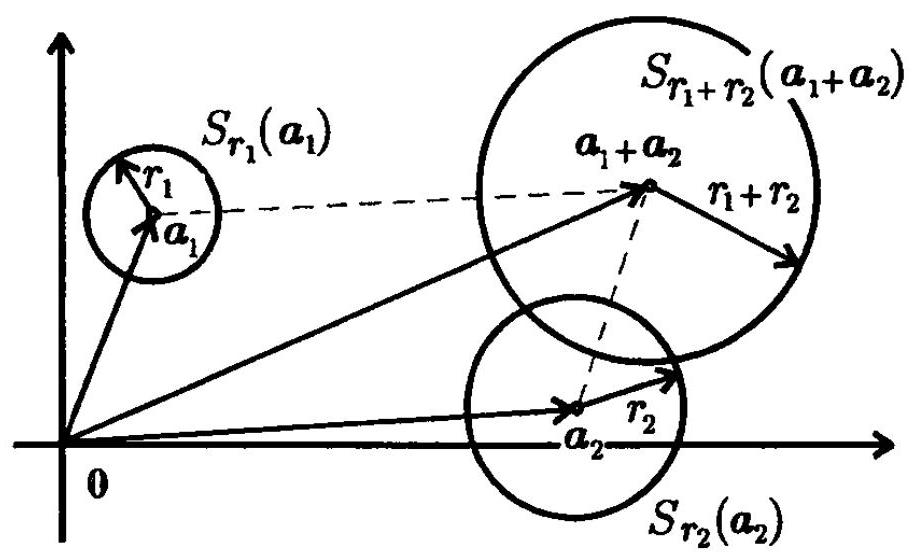
\includegraphics[max width=0.8\textwidth]{images/bo_d547okref24c73bgfch0_19_259_0_913_555_0.jpg}
\end{center}
\hspace*{3em} 

Рис. 2

т.е. при сложении двух шаров их радиусы суммируются и век- торы, задающие центры шаров, также суммируются (рис. 2).

Докажем этот факт, т.е. покажем, что множества в левой и правой частях формулы (2.5) совпадают. Если

\[
x \in  {S}_{{r}_{1}}\left( {a}_{1}\right)  + {S}_{{r}_{2}}\left( {a}_{2}\right) ,
\]

то по определению суммы двух множеств (2.4) х = f + g, где \(f \in  {S}_{{r}_{1}}\left( {a}_{1}\right) ,g \in  {S}_{{r}_{2}}\left( {a}_{2}\right)\) . Oтсюда по определению mapa (2.1) имеем

\[
\left\lVert \begin{array}{c} {f - {a}_{1}} \end{array} \right\rVert \leq  {r}_{1},\;\left\lVert \begin{array}{c} {g - {a}_{2}} \end{array} \right\rVert \leq  {r}_{2}.
\]

Учитывая эти неравенства, получаем

\[
\left\lVert \begin{array}{c} {\mathbf{x} - \left( {{\mathbf{a}}_{1} + {\mathbf{a}}_{2}}\right) } \end{array} \right\rVert = \left\lVert \begin{array}{c} {\mathbf{f} + \mathbf{g} - {\mathbf{a}}_{1} - {\mathbf{a}}_{2}} \end{array} \right\rVert \leq  \left\lVert \begin{array}{c} {\mathbf{f} - {\mathbf{a}}_{1}} \end{array} \right\rVert + \left\lVert \begin{array}{c} {\mathbf{g} - {\mathbf{a}}_{2}} \end{array} \right\rVert \leq  {r}_{1} + {r}_{2},
\]

т.е. \(x \in  {S}_{{r}_{1} + {r}_{2}}\left( {{a}_{1} + {a}_{2}}\right)\) и в одну сторону включение в формуле (2.5) доказано. Теперь, если хе ∈ \({S}_{{r}_{1} + {r}_{2}}\left( {{a}_{1} + {a}_{2}}\right)\) ,то

\[
\lambda  = \left\lVert \begin{array}{c} {\mathbf{x} - {\mathbf{a}}_{1} - {\mathbf{a}}_{2}} \end{array} \right\rVert \leq  {r}_{1} + {r}_{2}.
\]

ECли \(\lambda  = 0\) , to ovebmaho, \(q\) to

\[
\mathbf{x} = {\mathbf{a}}_{1} + {\mathbf{a}}_{2} \in  {S}_{{r}_{1}}\left( {\mathbf{a}}_{1}\right)  + {S}_{{r}_{2}}\left( {\mathbf{a}}_{2}\right) .
\]

Пусть теперь \(\lambda  \neq  0\) . Cymecтвуют такие положительные чис- ла \({\lambda }_{1} \leq  {r}_{1}\) и \({\lambda }_{2} \leq  {r}_{2}\) ,что \({\lambda }_{1} + {\lambda }_{2} = \lambda\) . Тогда

\[
f = {a}_{1} + \frac{{\lambda }_{1}}{\lambda }\left( {x - {a}_{1} - {a}_{2}}\right)  \in  {S}_{{r}_{1}}\left( {a}_{1}\right) ,
\]

\[
g = {a}_{2} + \frac{{\lambda }_{2}}{\lambda }\left( {x - {a}_{1} - {a}_{2}}\right)  \in  {S}_{{r}_{2}}\left( {a}_{2}\right)
\]

и \(x = f + g\) . Таким образом, \(x \in  {S}_{{r}_{1}}\left( {a}_{1}\right)  + {S}_{{r}_{2}}\left( {a}_{2}\right)\) и формула (2.5) доказана полностью. Из этой формулы при \({r}_{1} = r,{r}_{2} = 0\) , \({a}_{1} = 0,{a}_{2} = a\) c следует соот- ношение

\[
{S}_{r}\left( \mathbf{0}\right)  + \{ \mathbf{a}\}  = {S}_{r}\left( \mathbf{a}\right) . \tag{2.6}
\]

\begin{center}
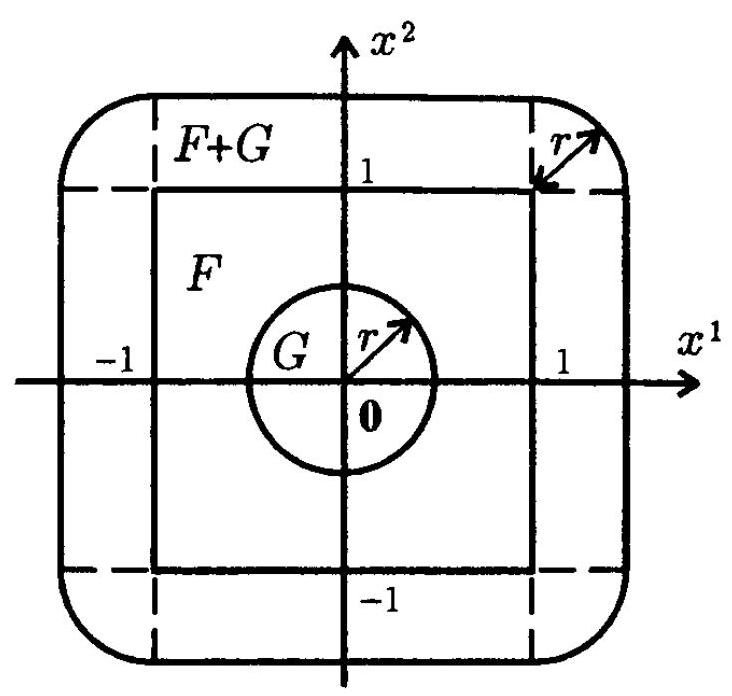
\includegraphics[max width=0.7\textwidth]{images/bo_d547okref24c73bgfch0_20_721_15_732_696_0.jpg}
\end{center}
\hspace*{3em} 

Рис. 3

Пример 3. Пусть мно- жество \(F -\) это квадрат на плоскости \({E}^{2}\) ,

\[
F = \left\{  {\mathbf{x} \in  {E}^{2} : }\right.
\]

\[
\left. {\left| {x}^{1}\right|  \leq  1,\left| {x}^{2}\right|  \leq  1}\right\}  ,
\]

а множество \(G\) - шар ради- yca \(r\) c центром в начале ко- ординат, \(G = {S}_{r}\left( 0\right)\) . Их сумма \(F + G\) изображена на рис. 3.

Операция алгебраической суммы для любых множеств F, G, \(P \in  \Omega \left( {E}^{n}\right)\) удовлетворяет следующим свойствам:

1) коммутативности: \(F + G = G + F\) ;

2) accoциативности: \(F + \left( {G + P}\right)  = \left( {F + G}\right)  + P\) ;

3) в пространстве Ω(E’) существует нулевой элемент \(\{ 0\}  : F + \{ 0\}  = F\) .

Доказательство этих свойств непосредственно следует из определения (2.4) алгебраической суммы и соответствующих свойств для векторов из пространства Е". Необходимо отме- тить, что если множество в состоит более чем из одной точки, то у такого множества F нет обратного элемента относительно введенной операции алгебраической суммы множеств, т.е. не су- ществует такого множества - \(F \in  \Omega \left( {E}^{n}\right)\) ,что \(F + \left( {-F}\right)  = \{ 0\}\) . Если же \(F = \{ \mathbf{f}\}\) , ro \(- F = \{  - \mathbf{f}\}\) .

Умножение множества на число. Произведением мно- жества \(F \in  \Omega \left( {E}^{n}\right)\) начисло \(\lambda\) называется множество

\[
G = {\lambda F} = \{ \mathbf{g} = \lambda \mathbf{f} : \mathbf{f} \in  F\} \tag{2.7}
\]

(рис. 4). В этом случае \(G \in  \Omega \left( {E}^{n}\right)\) , т.е. произведение множес- тва F ∈ \(\Omega \left( {E}^{n}\right)\) на произвольное число λ является непустым замкнутым и ограниченным множеством и, следовательно, не выводит из пространства \(\Omega \left( {E}^{n}\right)\) . Далее, если F — множество выпуклое, то и множество \(G = {\lambda F}\) также выпуклое. Эти факты доказываются так же просто, как и соответствующие свойства алгебраической суммы множеств (читателю предлагается сде- лать это самостоятельно).

\begin{center}
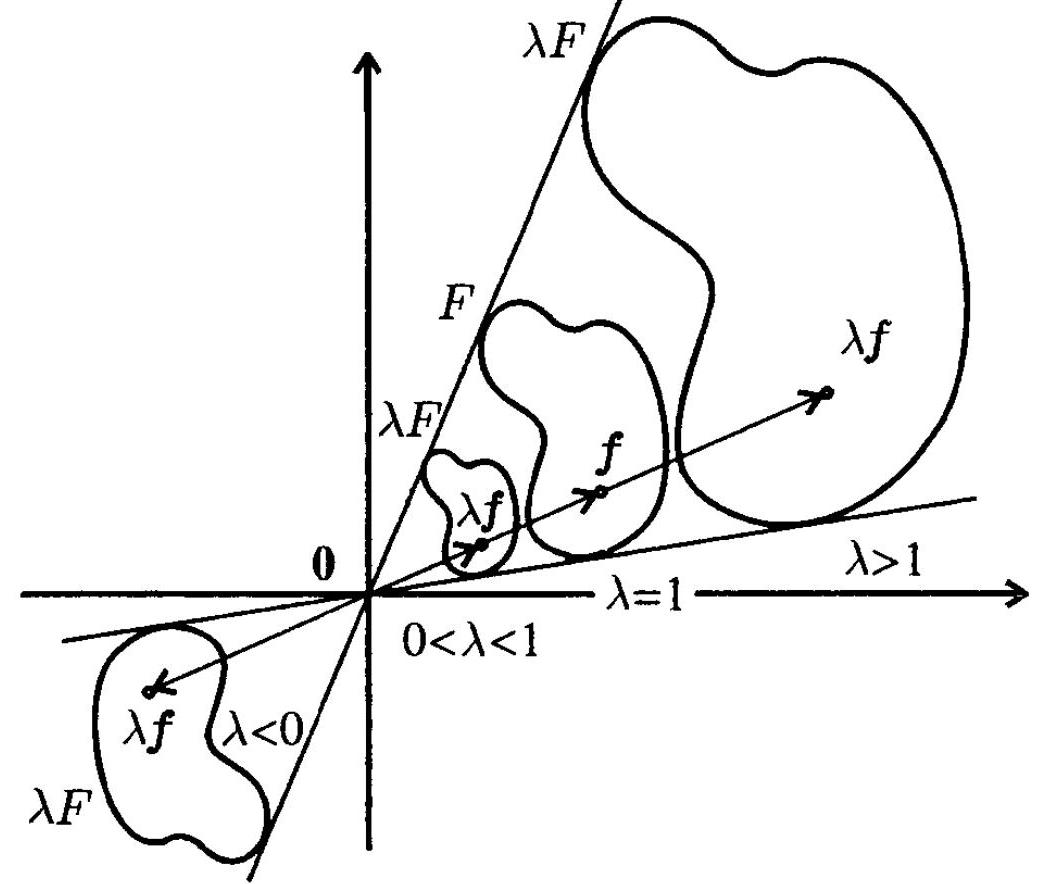
\includegraphics[max width=0.9\textwidth]{images/bo_d547okref24c73bgfch0_21_211_0_1042_884_0.jpg}
\end{center}
\hspace*{3em} 

Рис. 4

Пример 4. Докажем, что

\[
\lambda {S}_{r}\left( \mathbf{0}\right)  = {S}_{\left| \lambda \right| r}\left( \mathbf{0}\right) . \tag{2.8}
\]

Действительно, если g ∈ \(\lambda {S}_{r}\left( \mathbf{0}\right)\) , то g = \(\lambda \mathbf{f}\) , где f ∈ \({S}_{r}\left( \mathbf{0}\right)\) . B этом случае

\[
\parallel \mathbf{g}\parallel  = \parallel \lambda \mathbf{f}\parallel  = \left| \lambda \right|  \cdot  \parallel \mathbf{f}\parallel  \leq  \left| \lambda \right| r,
\]

т.е. \(g \in  {S}_{\left| \lambda \right| r}\left( 0\right)\) . Наоборот, ecли \(g \in  {S}_{\left| \lambda \right| r}\left( 0\right)\) и \(\lambda  \neq  0\) (при \(\lambda  = 0\) формула (2.8) очевидна), то \(\mathbf{f} = \frac{1}{\lambda }\mathbf{g} \in  {S}_{r}\left( \mathbf{0}\right)\) и \(\mathbf{g} = \lambda \mathbf{f}\) . Таким образом, \(g \in  {S}_{r}\left( 0\right)\) и формула (2.8) доказана.

Из формул (2.6) и (2.8) следует, что любой шар \$r(a) можно представить в виде

\[
{S}_{r}\left( \mathbf{a}\right)  = \{ \mathbf{a}\}  + r{S}_{1}\left( \mathbf{0}\right) .
\]

Непосредственно можно проверить, что для любых чисел \(\alpha ,\beta\) и любых двух множеств F, \(G \in  \Omega \left( {E}^{n}\right)\) выполняются сле- дующие свойства:

1) \(\alpha \left( {\beta F}\right)  = \left( {\alpha \beta }\right) F\)

2) \(1 \cdot  F = F\)

3) \(\alpha \left( {F + G}\right)  = {\alpha F} + {\alpha G}\) .

Эти свойства являются следствием соответствующих свойств векторов из пространства E".

Пространство \(\Omega \left( {E}^{n}\right)\) не является линейным пространством с операциями алгебраической суммы двух множеств и умножения множества на число хотя бы потому, что не у каждого элемента \(F \in  \Omega \left( {E}^{n}\right)\) ecть обратный элемент — \(F\) . Кроме того, не всегда выполняется необходимый для линейности закон дистрибутив- ности, т.е. не всегда выполняется равенство

\[
\left( {\alpha  + \beta }\right) F = {\alpha F} + {\beta F}. \tag{2.9}
\]

Приведем пример.

Пример 5. Пусть \(F = {S}_{1}\left( \mathbf{0}\right) ,\alpha  = 1,\beta  =  - 1\) . Тогда по формуле (2.8)

\[
{\alpha F} = 1 \cdot  {S}_{1}\left( \mathbf{0}\right)  = {S}_{1}\left( \mathbf{0}\right) ,\;{\beta F} =  - 1 \cdot  {S}_{1}\left( \mathbf{0}\right)  = {S}_{1}\left( \mathbf{0}\right) ,
\]

ивсилуформулы (2.5) \({\alpha F} + {\beta F} = {S}_{2}\left( \mathbf{0}\right)\) . Однако

\[
\left( {\alpha  + \beta }\right) F = \left( {1 - 1}\right) F = 0 \cdot  F = \{ 0\} .
\]

Таким образом, \{0\} ≠ S2(0) и формула (2.9) неверна.

Вместо равенства в формуле (2.9) справедливо лишь одно- стороннее включение

\[
\left( {\alpha  + \beta }\right) F \subset  {\alpha F} + {\beta F} \tag{2.10}
\]

Действительно, если х ∈ \(\left( {\alpha  + \beta }\right) F\) ,то по определению операции умножения на число (2.7) существует такой элемент f ∈ F, что

\[
\mathbf{x} = \left( {\alpha  + \beta }\right) \mathbf{f} = \alpha \mathbf{f} + \beta \mathbf{f}.
\]

Haree, tak kak \(\alpha \mathbf{f} \in  {\alpha F},\beta \mathbf{f} \in  {\beta F}\) , to

\[
\mathbf{x} = \alpha \mathbf{f} + \beta \mathbf{f} \in  {\alpha F} + {\beta F}
\]

и требуемое включение доказано.

Оказывается, что если α ≥ 0, β ≥ 0 и множество F выпук- ло, то формула (2.9) в этом случае справедлива. Докажем это. IIycth \(\alpha  \geq  0,\beta  \geq  0\) и \(\alpha  + \beta  \neq  0\) . II ри \(\alpha  + \beta  = 0\) имеем \(\alpha  = 0\) , \(\beta  = 0\) и формула (2.9) очевидна. В силу выпуклости множества \(F\) выполняется включение

\[
\frac{\alpha }{\alpha  + \beta }F + \frac{\beta }{\alpha  + \beta }F \subset  F. \tag{2.11}
\]

Действительно, пусть

\[
x \in  \frac{\alpha }{\alpha  + \beta }F + \frac{\beta }{\alpha  + \beta }F
\]

тогда существуют векторы \({f}_{1},{f}_{2} \in  F\) такие,что

\[
\mathbf{x} = \frac{\alpha }{\alpha  + \beta }{\mathbf{f}}_{1} + \frac{\beta }{\alpha  + \beta }{\mathbf{f}}_{2}.
\]

Далее, имеем

\[
\frac{\alpha }{\alpha  + \beta } \geq  0,\;\frac{\beta }{\alpha  + \beta } \geq  0,\;\frac{\alpha }{\alpha  + \beta } + \frac{\beta }{\alpha  + \beta } = 1.
\]

Учитывая выпуклость множества F, получаем, что x ∈ F и включение (2.11) доказано. Согласно свойству 3 операции умно- жения преобразуем включение (2.11) к виду αF+βF C (α+β)F. Отсюда из противоположного включения (2.10) следует равен- ство (2.9).

Рассмотрим подпространство conv \(\Omega \left( {E}^{n}\right)\) пространства \(\Omega \left( {E}^{n}\right)\) , cocoonщее из всех непустых выпуклых компактных под- множеств пространства E". Приведенные выше свойства опера- ций алгебраической суммы множеств и умножения множества на число показывают, что если рассматривать умножение вы- пуклых множеств только на неотрицательные числа, то для пространства conv \(\Omega \left( {E}^{n}\right)\) справедливы все аксиомы линейнос- ти, кроме аксиомы существования обратного элемента. В этом смысле пространство conv \(\Omega \left( {E}^{n}\right)\) напоминает выпуклый конус с вершиной в нуле, не совпадающий со всем пространством.

Образ множества при линейном преобразовании. IIycth \(F \in  \Omega \left( {E}^{n}\right)\) и в пространстве E" задано линейное пре- образование с помощью матрицы \(A\) (с действительными эле- ментами) размером \(n \times  n\) . Образом множества F при линейном преобразовании \(A\) называется множество

\[
G = {AF} = \{ \mathbf{g} = A\mathbf{f} : \mathbf{f} \in  F\} . \tag{2.12}
\]

\begin{center}
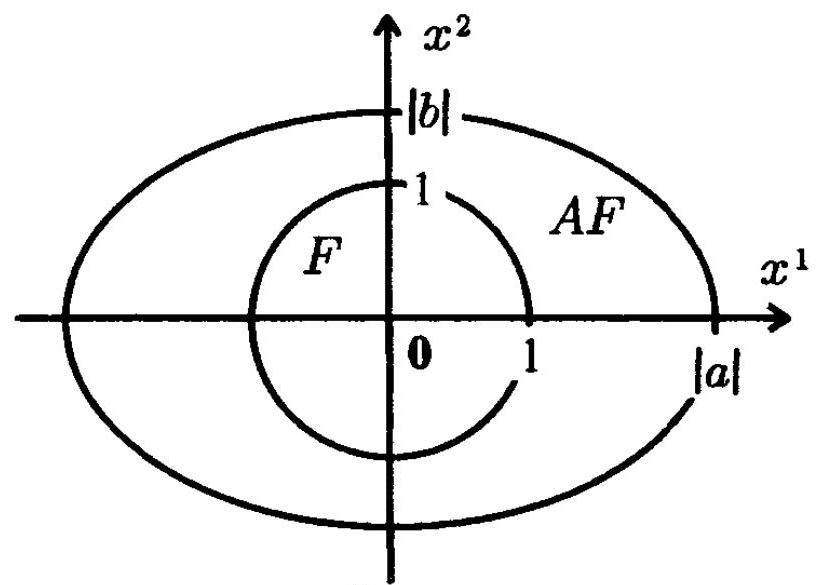
\includegraphics[max width=0.7\textwidth]{images/bo_d547okref24c73bgfch0_24_319_0_819_585_0.jpg}
\end{center}
\hspace*{3em} 

Рис. 5

Легко проверить, что \(G \in  \Omega \left( {E}^{n}\right)\) , т.е. образ множества \(F \in\) ∈ \(\Omega \left( {E}^{n}\right)\) при линейном преобразовании А является непустым, замкнутым и ограниченным множеством. Если F — выпуклое множество, то и множество G’ = AF также выпукло.

Пример 6. Пусть \(A = {\lambda E}\) ,где \(\lambda\) — некоторое число,а E — единичная матрица размером \(n \times  n\) . Тогда для произвольного вектора \(f \in  {E}^{n}\) имеем \({Af} = {\lambda Ef} = {\lambda f}\) . Cледовательно, образом \({AF}\) произвольного множества F при таком линейном преобразо- вании \(A = {\lambda E}\) будет множество \({\lambda F}\) . Таким образом, умножение множества на число является частным случаем линейного пре- образования при \(A = {\lambda E}\) .

IIpanep 7. Ilycth \(n = 2,F = {S}_{1}\left( 0\right)\) и матрица \(A\) имеет вид

\[
A = \left( \begin{array}{ll} a & 0 \\  0 & b \end{array}\right) .
\]

Легко показать, что единичный шар \({S}_{1}\left( 0\right)\) при таком линей- ном преобразовании А перейдет в эллипс

\[
{AF} = \left\{  {x \in  {E}^{2} : {\left( \frac{{x}^{1}}{a}\right) }^{2} + {\left( \frac{{x}^{2}}{b}\right) }^{2} \leq  1}\right\}  ,
\]

если \(a \neq  0,b \neq  0\left( {\mathrm{p}\text{ ис. 5),иливотрезок }}\right)\)

\[
{AF} = \left\{  {x \in  {E}^{2} : {x}^{1} = 0,\left| {x}^{2}\right|  \leq  \left| b\right| }\right\}  ,
\]

если а \(= 0,b \neq  0\) ,иливотрезок

\[
{AF} = \left\{  {\mathbf{x} \in  {E}^{2} : {x}^{2} = 0,\left| {x}^{1}\right|  \leq  \left| a\right| }\right\}  ,
\]

если \(a \neq  0,b = 0\) .

Для любых матриц \(A,B\) и любых множеств F, \(G \in  \Omega \left( {E}^{n}\right)\) выполняются следующие свойства:

1) \(A\left( {BF}\right)  = \left( {AB}\right) F\)

2) \({EF} = F\)

3) \(A\left( {F + G}\right)  = {AF} + {AG}\) ;

4) \(\left( {A + B}\right) F \subset  {AF} + {BF}\) .

Свойства 1 — 3 являются следствием соответствующих свойств векторов из пространства Е". Свойство 4 доказывается так же, как и соответствующее включение (2.10) для операции умножения множества на число.

Хаусдорфово расстояние. В пространстве Ω(Ег) можно ввести метрику, или расстояние, h(F, G) между двумя множес- твами \(F,G \in  \Omega \left( {E}^{n}\right)\) по формуле

\[
h\left( {F,G}\right)  = \min \{ r \geq  0 : F \subset  G + {S}_{r}\left( 0\right) ,G \subset  F + {S}_{r}\left( 0\right) \} . \tag{2.13}
\]

Таким образом, расстоянием между двумя множествами яв- ляется наименьшее из положительных чисел r, для которых выполняются одновременно два включения

\[
F \subset  G + {S}_{r}\left( \mathbf{0}\right) ,\;G \subset  F + {S}_{r}\left( \mathbf{0}\right) . \tag{2.14}
\]

Эта метрика называется хаусдорфовой.

Рассмотрим пример расстояния \(h\left( {F,G}\right)\) .

Пример 8. Пусть \(F = \{ 0\} ,G = {S}_{1}\left( 0\right)\) — два множества в пространстве E". Первое из включений (2.14) в данном случае выполняется всегда, так как \{0\} ⊂ S1(0) + Sr(0) для любых \(r \geq  0\) . Второе включение \({S}_{1}\left( 0\right)  \subset  {S}_{r}\left( 0\right)\) выполняется, если r ≥1. Таким образом, минимальным числом r, для которого одновре- менно выполняются оба включения (2.14), будет число r = 1, т.е. в данном примере \(h\left( {F,G}\right)  = 1\) .

Пример 9. Докажем, что

\[
h\left( {F,\{ 0\} }\right)  = \left| F\right| .
\]

Действительно, по определению расстояние h(F, \{0\}) — ми- нимальное из чисел r ≥ 0, для которых выполняются одновре- менно два включения

\[
F \subset  \{ \mathbf{0}\}  + {S}_{r}\left( \mathbf{0}\right) ,\;\{ \mathbf{0}\}  \subset  F + {S}_{r}\left( \mathbf{0}\right) .
\]

Выполнение первого включения для некоторого \(r \geq  0\) вле- чет за собой выполнение второго включения. Таким образом, \(h\left( {F,\{ 0\} }\right)\) ecть минимальное число r ≥0, anя которого выпол- нено включение \(F \subset  {S}_{r}\left( 0\right)\) , т.е. это — модуль |F| множества \(F\) .

Докажем, что функция \(h\left( {F,G}\right)\) действительно является рас- стоянием, т.е. удовлетворяет всем аксиомам расстояния. Для этого нужно доказать, что для любых множеств F, G, P ∈ Ω(Er) выполняются следующие свойства:

1) \(h\left( {F,G}\right)  \geq  0\) ;

2) \(h\left( {F,G}\right)  = 0\) тогда и только тогда, когда \(F = G\) ;

3) \(h\left( {F,G}\right)  = h\left( {G,F}\right)\) ;

4) \(h\left( {F,G}\right)  \leq  h\left( {F,P}\right)  + h\left( {P,G}\right)\) .

Проверка первых трех свойств не представляет труднос- тей, поэтому докажем только свойство 4. Пусть \(h\left( {F,P}\right)  = \alpha\) , \(h\left( {P,G}\right)  = \beta\) . Тогда согласно формуле (2.13) выполняются сле- дующие включения:

\[
F \subset  P + {S}_{\alpha }\left( 0\right) ,\;P \subset  F + {S}_{\alpha }\left( 0\right) ,
\]

\[
P \subset  G + {S}_{\beta }\left( \mathbf{0}\right) ,\;G \subset  P + {S}_{\beta }\left( \mathbf{0}\right) .
\]

Комбинируя эти включения, получаем

\[
F \subset  P + {S}_{\alpha }\left( 0\right)  \subset  G + {S}_{\beta }\left( 0\right)  + {S}_{\alpha }\left( 0\right)  = G + {S}_{\alpha  + \beta }\left( 0\right) .
\]

Аналогичным образом выводится включение G C F + \(+ {S}_{\alpha  + \beta }\left( 0\right)\) . A так как хаусдорфово расстояние \(h\left( {F,G}\right)\) — наи- меньшее из чисел, для которых выполняются одновременно по- следние два включения, то \(h\left( {F,G}\right)  \leq  \alpha  + \beta\) . Тем самым свой- ство 4 доказано.

\section*{2.3. Задачи}

1. Выполняется ли для любого множества F ∈ Ω( \({E}^{n}\) ) равен- ство F + F = 2F ?

\({2}^{ * }\) . Множество \(F \in  \Omega \left( {E}^{n}\right)\) обладает тем свойством,что для любых двух его точек х, ку ес не средина отрезка хд хд мели. няющего эти точки, принадлежит множеству F. Докажите, что множество \(F\) выпукло.

\HRule

*Звездочкой отмечены задачи повышенной сложности.

\HRule

\({3}^{ * }\) . Для множества F ∈ \(\Omega \left( {E}^{n}\right)\) существует такое число λ, \(0 < \lambda  < 1\) ,что выполняется включение

\[
{\lambda F} + \left( {1 - \lambda }\right) F \subset  F.
\]

Докажите, что множество F выпукло.

4. Множества \({F}_{1},{F}_{2},{G}_{1},{G}_{2} \in  \Omega \left( {E}^{n}\right)\) удовлетворяют вклю- чениям

\[
{F}_{1} \subset  {F}_{2},\;{G}_{1} \subset  {G}_{2}.
\]

Для произвольного числа λ и произвольной матрицы \(A\) разме- ром \(n \times  n\) докажите включения:

\[
\text{ 1) }{F}_{1} + {G}_{1} \subset  {F}_{2} + {G}_{2}
\]

\[
\text{ 2) }\lambda {F}_{1} \subset  \lambda {F}_{2}
\]

\[
\text{ 3) }A{F}_{1} \subset  A{F}_{2}\text{ . }
\]

5. Hañдите образ множества

\[
F = \left\{  {x \in  {E}^{2} : \left| {x}^{1}\right|  \leq  1,\left| {x}^{2}\right|  \leq  1}\right\}
\]

при линейных преобразованиях \(A\) следующего вида:

\[
\text{ 1) }A = \left( \begin{array}{ll} a & 0 \\  0 & b \end{array}\right) ;\;\text{ 2) }A = \left( \begin{array}{cc} 0 & \frac{\sqrt{2}}{2} \\  \frac{\sqrt{2}}{2} & 0 \end{array}\right) \text{ ; }
\]

\[
\text{ 3) }A = \left( \begin{array}{rr} \sin \varphi & \cos \varphi \\   - \cos \varphi & \sin \varphi  \end{array}\right) \text{ . }
\]

6. Haßдите расстояние \(h\left( {F,G}\right)\) мехдумножеством

\[
F = \left\{  {x \in  {E}^{2} : \left| {x}^{1}\right|  \leq  1,\left| {x}^{2}\right|  \leq  1}\right\}
\]

и множествами G ∈ Ω(E’) следующего вида:

1) \(G = {S}_{r}\left( 0\right)\) . При каком r это расстояние минимально?

2) \(G = \{ g\}\) . При каком g это расстояние минимально?

7. Найдите расстояние h(F, G) между двумя произвольными шарами \(F = {S}_{{r}_{1}}\left( {a}_{1}\right)\) и \(G = {S}_{{r}_{2}}\left( {a}_{2}\right)\) в пространстве E".

8. Найдите расстояние h(F, G) между множествами

\[
F = \left\{  {x \in  {E}^{2} : {\left( \frac{{x}^{1}}{a}\right) }^{2} + {\left( \frac{{x}^{2}}{b}\right) }^{2} \leq  1}\right\}  ,\;a \neq  0,b \neq  0;
\]

\[
G = \left\{  {x \in  {E}^{2} : {\left( \frac{{x}^{1}}{c}\right) }^{2} + {\left( \frac{{x}^{2}}{d}\right) }^{2} \leq  1}\right\}  ,\;c \neq  0,d \neq  0.
\]

\section*{JIEKIIИЯ 3}

\begin{itemize}\relax
\item\relax Опорная функция и ее основные свойства.
\end{itemize}

\begin{itemize}\relax
\item\relax Опорный вектор, опорное множество, опорная ги- перплоскость.
\end{itemize}

\begin{itemize}\relax
\item\relax Выпуклая оболочка множества.
\end{itemize}

\section*{3.1. Опорные функции}

Пусть задано некоторое множество \(F \in  \Omega \left( {E}^{n}\right)\) . Опорной функцией множества F называется скалярная функция \(c\left( {F,\psi }\right)\) векторного аргумента ψ с Ег", определяемая условием

\[
c\left( {F,\psi }\right)  = \mathop{\max }\limits_{{f \in  F}}\langle f,\psi \rangle , \tag{3.1}
\]

где \(\langle \mathbf{f},\mathbf{\psi }\rangle\) — скалярное произведение векторов \(\mathbf{f} = \left( {{f}^{1},\ldots ,{f}^{n}}\right)\) и и \(\psi  = \left( {{\psi }^{1},\ldots ,{\psi }^{n}}\right)\) ,заданное формулой

\[
\langle \mathbf{f},\psi \rangle  = \mathop{\sum }\limits_{{i = 1}}^{n}{f}^{i}{\psi }^{i}
\]

Множество F также считается одним из аргументов функции \(c\left( {F,\psi }\right)\) . Зафиксируем множество F. Функция \(c\left( {F,\psi }\right)\) как функ- ция аргумента ψ отображает пространство Е" в числовую ось \({E}^{1}\) . Запишем этот факт в виде символов следующим образом:

\[
c\left( {F, \cdot  }\right)  : {E}^{n} \rightarrow  {E}^{1}.
\]

Ясно, что максимум в правой части равенства (3.1) достига- ется, так как скалярное произведение \(\langle \mathbf{f},\mathbf{\psi }\rangle\) непрерывно по \(\mathbf{\psi }\) , а множество \(F\) компактно. Пусть му \({\psi }_{0} \in  {E}^{n} -\) некоторый фик- сированный вектор, а \({\mathbf{f}}_{0}\) — один из векторов множества F, на котором достигается максимум в определении опорной функции (3.1) для вектора ф \(= {\psi }_{0}\) ,т.е. выполняется равенство

\[
\left\langle  {{\mathbf{f}}_{0},{\mathbf{\psi }}_{0}}\right\rangle   = \mathop{\max }\limits_{{\mathbf{f} \in  F}}\left\langle  {\mathbf{f},{\mathbf{\psi }}_{0}}\right\rangle   = c\left( {F,{\mathbf{\psi }}_{0}}\right) . \tag{3.2}
\]

\begin{center}
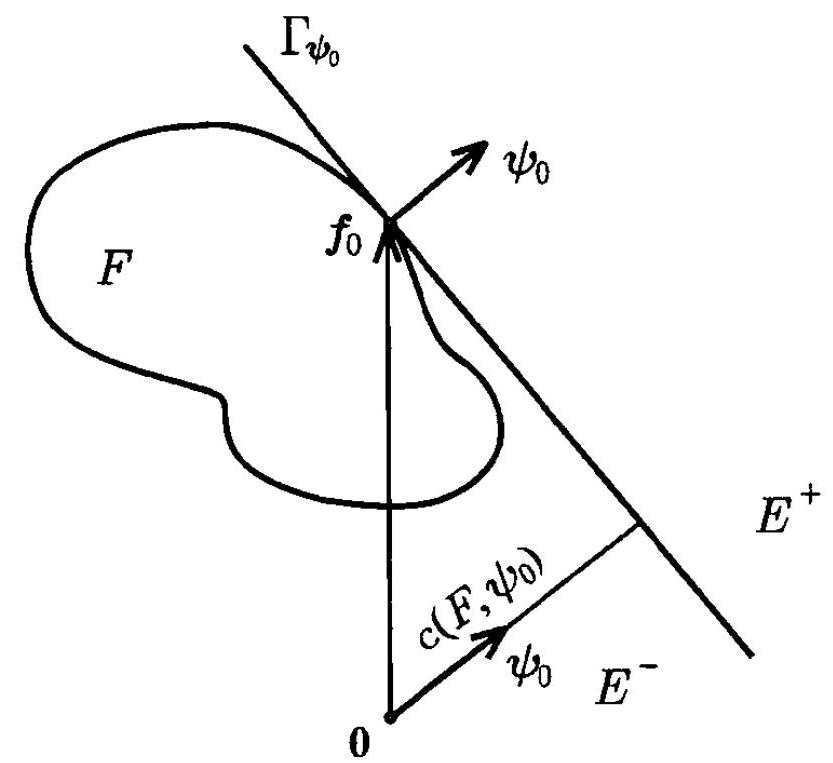
\includegraphics[max width=0.7\textwidth]{images/bo_d547okref24c73bgfch0_29_310_0_833_763_0.jpg}
\end{center}
\hspace*{3em} 

Рис. 6

В этом случае вектор \({\mathbf{\psi }}_{0}\) называется опорным вектором к множеству \(F\) в точке \({\mathbf{f}}_{0}\) , a совокупность \(\mathcal{U}\left( {F,{\mathbf{\psi }}_{0}}\right)\) всех векторов \({\mathbf{f}}_{0} \in  F\) , yдовлетворяющих равенству (3.2),называется опорным множеством к множеству \(F\) в направлении вектора \({\mathbf{\psi }}_{0}\) . Гипер- плоскость \({\Gamma }_{{\psi }_{0}}\) в пространстве E", onределяемая соотношением

\[
{\Gamma }_{{\psi }_{0}} = \left\{  {\mathbf{x} \in  {E}^{n} : \left\langle  {\mathbf{x},{\mathbf{\psi }}_{0}}\right\rangle   = \left\langle  {{\mathbf{f}}_{0},{\mathbf{\psi }}_{0}}\right\rangle  }\right\}  ,
\]

называется опорной гиперплоскостью к множеству \(F\) в направ- лении вектора ф \({}_{0}\) (рис. 6 и 7). Для опорного множества И( F , ψ ) справедливо представление

\[
\mathcal{U}\left( {F,{\psi }_{0}}\right)  = F \cap  {\Gamma }_{{\psi }_{0}}.
\]

Гиперплоскость \({\Gamma }_{{\psi }_{0}}\) разбивает все пространство \({E}^{n}\) на два полупространства \({E}^{ + }\) и \({E}^{ - }\) . Множество \(F\) лежит в отрицатель- ном полупространстве \({E}^{ - }\) относительно вектора \({\mathbf{\psi }}_{0}\) ,так как для всех точек \(f \in  F\) выполняется неравенство

\[
\left\langle  {\mathbf{f},{\mathbf{\psi }}_{0}}\right\rangle   \leq  \left\langle  {{\mathbf{f}}_{0},{\mathbf{\psi }}_{0}}\right\rangle  .
\]

Если \({\mathbf{\psi }}_{0} \in  S\) , т.е. вектор \({\mathbf{\psi }}_{0}\) имеет единичную длину, то ве- личина \(c\left( {F,{\mathbf{\psi }}_{0}}\right)  = \left\langle  {{\mathbf{f}}_{0},{\mathbf{\psi }}_{0}}\right\rangle\) — расстояние от начала координат 0 до гиперплоскости \({\Gamma }_{{\psi }_{0}}\) ,взятое со знаком плюс, если начало координат лежит в отрицательном полупространстве E- отно- сительно вектора фи (см. рис. 6), и со знаком минус, если начало координат лежит в положительном полупространстве E+ (см. рис. 7). Таков геометрический смысл опорной функции.

\begin{center}
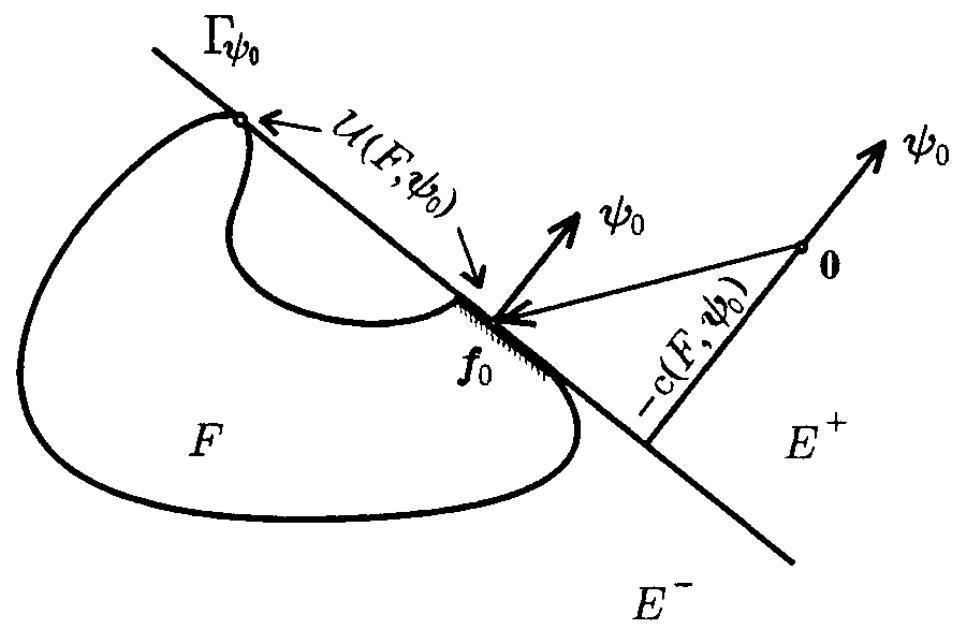
\includegraphics[max width=0.9\textwidth]{images/bo_d547okref24c73bgfch0_30_248_0_964_630_0.jpg}
\end{center}
\hspace*{3em} 

Рис. 7

Приведем несколько примеров нахождения опорных функ- ций.

Пример 1. Пусть множество F состоит из единственной точки,т.е. \(F = \{ f\}\) . Тогда очевидно, что

\[
c\left( {\{ \mathbf{f}\} ,\psi }\right)  = \langle \mathbf{f},\psi \rangle . \tag{3.3}
\]

Пример 2. Вычислим опорную функцию единичного шара в пространстве \({E}^{n}\) c центром в начале координат. Если F = \({S}_{1}\left( \mathbf{0}\right)\) , то ясно, что максимум в формуле (3.1) достигается на векторе \({\mathbf{f}}_{0} = \frac{\mathbf{\psi }}{\parallel \mathbf{\psi }\parallel }\) . Тогда имеем

\[
c\left( {{S}_{1}\left( \mathbf{0}\right) ,\psi }\right)  = \left\langle  {{\mathbf{f}}_{0},\psi }\right\rangle   = \left\langle  {\frac{\psi }{\parallel \psi \parallel },\psi }\right\rangle   = \parallel \psi \parallel . \tag{3.4}
\]

Пример 3. Вычислим опорную функцию квадрата F на плоскости \({E}^{2}\) , заданного условием

\[
F = \left\{  {\mathbf{x} \in  {E}^{2} : \left| {x}^{1}\right|  \leq  1,\left| {x}^{2}\right|  \leq  1}\right\}  .
\]

Если вектор \(\psi  = \left( {{\psi }^{1},{\psi }^{2}}\right)\) принадлежит первому квадранту на плоскости \({E}^{2}\) , т.е. \({\psi }^{1} \geq  0,{\psi }^{2} \geq  0\) , то максимум в формуле (3.1) достигается на векторе \({f}^{0} = \left( {1,1}\right)\) . Таким образом,

\[
c\left( {F,\psi }\right)  = \left\langle  {{\mathbf{f}}_{0},\psi }\right\rangle   = {\psi }^{1} + {\psi }^{2}.
\]

Далее, если вектор ψ принадлежит второму квадранту, т.е. \({\psi }^{1} \leq  0,{\psi }^{2} \geq  0\) , ro максимум в формуле (3.1) достигается на векторе \({\mathbf{f}}_{0} = \left( {-1,1}\right)\) и \(c\left( {F,\mathbf{\psi }}\right)  =  - {\psi }^{1} + {\psi }^{2}\) . Аналогично для векторов ф из третьего и четвертого квадрантов получаем co- ответствующие значения опорной функции \(c\left( {F,\psi }\right)  =  - {\psi }^{1} - {\psi }^{2}\) и \(c\left( {F,\psi }\right)  = {\psi }^{1} - {\psi }^{2}\) . Объединяя все выражения опорной функции, получаем окончательно

\[
c\left( {F,\psi }\right)  = \left| {\psi }^{1}\right|  + \left| {\psi }^{2}\right| . \tag{3.5}
\]

\section*{3.2. Свойства опорных функций}

Свойство 1. Опорная функция \(c\left( {F, \cdot  }\right)  : {E}^{n} \rightarrow  {E}^{1}\) положи- тельно однородна, т.е.

\[
c\left( {F,{\lambda \psi }}\right)  = {\lambda c}\left( {F,\psi }\right)
\]

для любого вектора ψ ∈ Е" и любого числа λ ≥ 0. В частнос- \({mu},c\left( {F,\mathbf{0}}\right)  = 0\) .

Доказательство этого свойства непосредственно следу- ет из определения опорной функции (3.1) и свойств максимума. Действительно, справедливы равенства

\[
c\left( {F,{\lambda \psi }}\right)  = \mathop{\max }\limits_{{\mathbf{f} \in  F}}\langle \mathbf{f},\lambda \mathbf{\psi }\rangle  = \lambda \mathop{\max }\limits_{{\mathbf{f} \in  F}}\langle \mathbf{f},\mathbf{\psi }\rangle  = {\lambda c}\left( {F,\mathbf{\psi }}\right) .
\]

Свойство 2. Для любых двух векторов ц’нх, н2 ее в попр- ная функция удовлетворяет неравенству

\[
c\left( {F,{\psi }_{1} + {\psi }_{2}}\right)  \leq  c\left( {F,{\psi }_{1}}\right)  + c\left( {F,{\psi }_{2}}\right) .
\]

Доказательство этого свойства также выводится непо- средственно из определения опорной функции и свойств макси- мума. Действительно, имеем

\[
c\left( {F,{\psi }_{1} + {\psi }_{2}}\right)  = \mathop{\max }\limits_{{f \in  F}}\left\langle  {f,{\psi }_{1} + {\psi }_{2}}\right\rangle   \leq  \mathop{\max }\limits_{{f \in  F}}\left\langle  {f,{\psi }_{1}}\right\rangle   + \mathop{\max }\limits_{{f \in  F}}\left\langle  {f,{\psi }_{2}}\right\rangle   =
\]

\[
= c\left( {F,{\psi }_{1}}\right)  + c\left( {F,{\psi }_{2}}\right) .
\]

Функция \(f : {E}^{n} \rightarrow  {E}^{1}\) называется выпуклой, если для любых двух точек \({x}_{1},{x}_{2} \in  {E}^{n}\) и любого числа 0 ≤ λ<1 выполняется неравенство

\[
f\left( {\lambda {\mathbf{x}}_{1} + \left( {1 - \lambda }\right) {\mathbf{x}}_{2}}\right)  \leq  {\lambda f}\left( {\mathbf{x}}_{1}\right)  + \left( {1 - \lambda }\right) f\left( {\mathbf{x}}_{2}\right) .
\]

Следствие свойств 1 и 2. Опорная функция \(c\left( {F, \cdot  }\right)  : {E}^{n} \rightarrow \; \rightarrow  {E}^{1}\) является выпуклой.

Действительно, из свойств 2 и 1 следует, что для любых двух векторов \({\psi }_{1},{\psi }_{2} \in  {E}^{n}\) и любого числа 0 ≤ \(\lambda  \leq  1\) cnpaведливо соотношение

\[
c\left( {F,\lambda {\psi }_{1} + \left( {1 - \lambda }\right) {\psi }_{2}}\right)  \leq  c\left( {F,\lambda {\psi }_{1}}\right)  + c\left( {F,\left( {1 - \lambda }\right) {\psi }_{2}}\right)  =
\]

\[
= {\lambda c}\left( {F,{\psi }_{1}}\right)  + \left( {1 - \lambda }\right) c\left( {F,{\psi }_{2}}\right) .
\]

Свойство 3. Пусть F, G ∈ Ω( \({E}^{n}\) ). Тогда опорная функция \(c\left( {F + G,\psi }\right) {cy}.{\text{ м }\text{ ы }}\;F + G\;p\) авняется сумме двух опорных функций \(c\left( {F,\psi }\right) u \subset  c\left( {G,\psi }\right) ,m\) . e.

\[
c\left( {F + G,\psi }\right)  = c\left( {F,\psi }\right)  + c\left( {G,\psi }\right) .
\]

Доказательство. По определению суммы двух множеств (см. лекцию 2) имеем

\[
F + G = \{ \mathbf{x} = \mathbf{f} + \mathbf{g} : \mathbf{f} \in  F,\mathbf{g} \in  G\} .
\]

Теперь воспользуемся определением опорной функции (3.1). Получаем

\[
c\left( {F + G}\right)  = \mathop{\max }\limits_{{\mathbf{x} \in  F + G}}\langle \mathbf{x},\mathbf{\psi }\rangle  = \mathop{\max }\limits_{{\mathbf{f} \in  F,\mathbf{g} \in  G}}\langle \mathbf{f} + \mathbf{g},\mathbf{\psi }\rangle  =
\]

\[
= \mathop{\max }\limits_{{\mathbf{f} \in  F}}\langle \mathbf{f},\mathbf{\psi }\rangle  + \mathop{\max }\limits_{{\mathbf{g} \in  G}}\langle \mathbf{g},\mathbf{\psi }\rangle  = c\left( {F,\mathbf{\psi }}\right)  + c\left( {G,\mathbf{\psi }}\right) .
\]

Доказательство свойства 3 завершено.

Пусть теперь \(A -\) матрица размером \(n \times  n\) , a \(f \in  \Omega \left( {E}^{n}\right)\) . Образ АF множества F при линейном преобразовании А опре- деляется формулой (см. лекцию 2)

\[
{AF} = \left\{  {\mathbf{x} \in  {E}^{n} : \mathbf{x} = {AF},\mathbf{f} \in  F}\right\}  . \tag{3.6}
\]

Посмотрим, как выражается опорная функция образа мно- жества \(F\) при линейном преобразовании.

Свойство 4. Пусть А — матрица размером n × n, a \(F \in  \Omega \left( {E}^{n}\right)\) . Toгда

\[
c\left( {{AF},\psi }\right)  = c\left( {F,{A}^{ * }\psi }\right) ,
\]

где A* — матрица, сопряженная с матрицей А.

Доказательство этого свойства непосредственно следует из определения опорной функции (3.1) и образа множества (3.6). Действительно,

\[
c\left( {{AF},\psi }\right)  = \mathop{\max }\limits_{{x \in  {AF}}}\langle x,\psi \rangle  = \mathop{\max }\limits_{{f \in  F}}\langle {Af},\psi \rangle  = \mathop{\max }\limits_{{f \in  F}}\left\langle  {f,{A}^{ * }\psi }\right\rangle  .
\]

Свойство 5. Пусть F ∈ Ω(E \({}^{n}\) ), а λ — произвольное число. Tozda

\[
c\left( {{\lambda F},\psi }\right)  = c\left( {F,{\lambda \psi }}\right) .
\]

Это свойство является частным случаем свойства 4, когда матрица \(A\) имеет вид \(A = {\lambda E}\) ,где \(E\) — единичная матрица размером \(n \times  n\) .

Следствие. Опорная функция \(c\left( {F,\psi }\right)\) положительно одно- родна по первому аргументу F, т.е.

\[
c\left( {{\lambda F},\psi }\right)  = {\lambda c}\left( {F,\psi }\right)
\]

для любого числа λ ≥0.

Для доказательства этого следствия достаточно воспользо- ваться свойством 1.

Пример 4. Вычислим опорную функцию произвольного ша- pa \({S}_{r}\left( \mathbf{a}\right)\) в пространстве E". В лекции 2 было показано, что шар \({S}_{r}\left( \mathbf{a}\right)\) можно представить в виде

\[
{S}_{r}\left( a\right)  = \{ a\}  + r{S}_{1}\left( 0\right) .
\]

Опорные функции множества \{a\} и единичного шара \({S}_{1}\left( 0\right)\) уже вычислены (см. формулы (3.3) и (3.4)). Используя свойство 3 и следствие свойства 5, получаем

\[
c\left( {{S}_{r}\left( a\right) ,\psi }\right)  = c\left( {\{ a\}  + r{S}_{1}\left( 0\right) ,\psi }\right)  = c\left( {\{ a\} ,\psi }\right)  + {rc}\left( {{S}_{1}\left( 0\right) ,\psi }\right)  =
\]

\[
= \langle \mathbf{a},\mathbf{\psi }\rangle  + r\parallel \mathbf{\psi }\parallel .
\]

Пример 5. Вычислим опорную функцию произвольного прямоугольника \(G\) на плоскости \({E}^{2}\) co сторонами, параллель- ными осям координат. Пусть этот прямоугольник задан в виде

\[
G = \left\{  {\mathbf{x} \in  {E}^{2} : {a}^{1} \leq  {x}^{1} \leq  {b}^{1},{a}^{2} \leq  {x}^{2} \leq  {b}^{2}}\right\}  .
\]

Получим прямоугольник \(G\) изквадрата

\[
F = \left\{  {\mathbf{x} \in  {E}^{2} : \left| {x}^{1}\right|  \leq  1,\left| {x}^{2}\right|  \leq  1}\right\}  ,
\]

данного в примере 3, при помощи соответствующего сдвига и линейного преобразования (растяжения). Тогда справедливо ра- венство

\[
G = \left\{  \left( {\frac{{b}^{1} + {a}^{1}}{2},\frac{{b}^{2} + {a}^{2}}{2}}\right) \right\}   + \left( \begin{array}{cc} \frac{{b}^{1} - {a}^{1}}{2} & 0 \\  0 & \frac{{b}^{2} - {a}^{2}}{2} \end{array}\right) F.
\]

Далее согласно свойствам Зичи формулам (3.3) и (3.5) имеем

\[
c\left( {G,\psi }\right)  = \frac{{b}^{1} + {a}^{1}}{2}{\psi }^{1} + \frac{{b}^{2} + {a}^{2}}{2}{\psi }^{2} + \frac{{b}^{1} - {a}^{1}}{2}\left| {\psi }^{1}\right|  + \frac{{b}^{2} - {a}^{2}}{2}\left| {\psi }^{2}\right| .
\]

Свойство 6. Пусть G, F ∈ Ω(E \({}^{n}\) ). Если выполняется вклю- чение \(G \subset  F\) , mo для любого вектора ψ ∈ \({E}^{n}\) cnpaведливо неравенство

\[
c\left( {G,\psi }\right)  \leq  c\left( {F,\psi }\right) .
\]

Доказательство непосредственно следует из определения опорной функции (3.1). Действительно, имеем

\[
c\left( {G,\psi }\right)  = \mathop{\max }\limits_{{g \in  G}}\langle g,\psi \rangle  \leq  \mathop{\max }\limits_{{f \in  F}}\langle f,\psi \rangle  = c\left( {F,\psi }\right) .
\]

Следствие. Пусть F ∈ Ω(Er). Если точка флринадлежит множеству \(F\) , т.е. \({f}_{\Omega } \in  F\) , то для любого вектора ψ ∈ \({E}^{n}\) выполняется неравенство

\[
\langle f,\psi \rangle  \leq  c\left( {F,\psi }\right) .
\]

Для получения этого следствия достаточно положить \(G = \left\{  {f}_{0}\right\}\) .

Для вывода дальнейших свойств опорных функций необхо- димо знание некоторых свойств выпуклой оболочки множества conv \(F\) .

\section*{3.3. Выпуклая оболочка множества}

Множество \(F \subset  {E}^{n}\) называется выпуклым (см. лекцию 2), если для любых двух точек х, ку с я б отрезок, соединяю- щий эти точки, содержится в множестве F, или, что то же самое, если для любого числа 0 ≤ λ ≤ 1 выполняется усло- вие \(\lambda {\mathbf{x}}_{1} + \left( {1 - \lambda }\right) {\mathbf{x}}_{2} \in  F\) . Ясно, что пересечение любого числа выпуклых множеств снова будет множеством выпуклым.

Оказывается, если n — размерность про- странства \({E}^{n}\) , то выпук- лая оболочка conv \(F\) мно- жества \(F \subset  {E}^{n}\) совпадает

\begin{center}
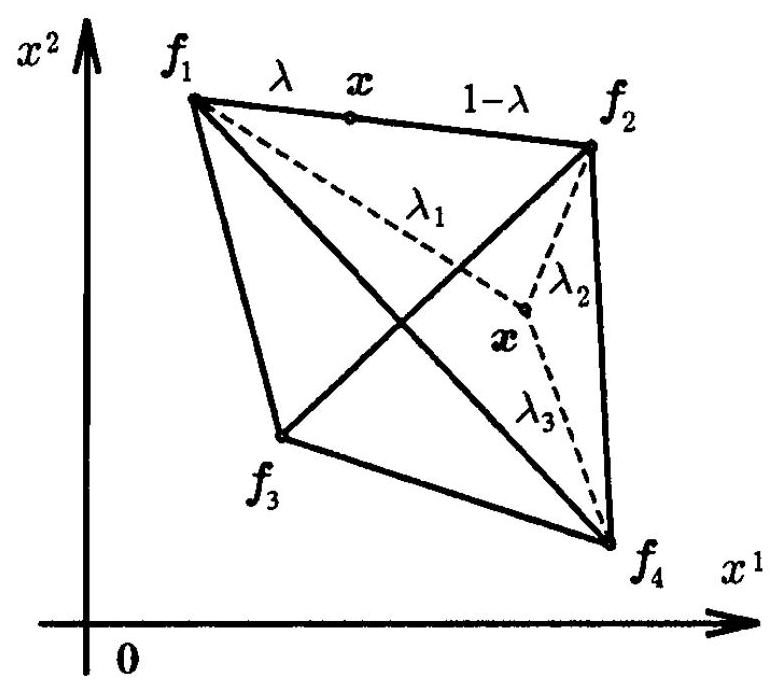
\includegraphics[max width=0.7\textwidth]{images/bo_d547okref24c73bgfch0_35_30_11_770_688_0.jpg}
\end{center}
\hspace*{3em} 

Рис. 8

c совокупностью всех точек вида

Выпуклой оболочкой conv \(F\) называется наи- меньшее выпуклое мно- жество, содержащее мно- жество F. Ясно, что conv \(F\) ecть пересечение всех выпуклых множеств, содержащих множество \(F\) . Если множество \(F\) вы- пукло, то conv \(F = F\) .

\[
\mathbf{x} = {\lambda }_{1}{\mathbf{x}}_{1} + \ldots  + {\lambda }_{n + 1}{\mathbf{x}}_{n + 1},\;{\mathbf{x}}_{i} \in  F,\;{\lambda }_{i} \geq  0,
\]

\[
{\lambda }_{1} + \ldots  + {\lambda }_{n + 1} = 1 \tag{3.7}
\]

В этом случае говорят, что точка х является выпуклой комбина- queй точек х, п., п. Доказательство этого факта приведено в разд. Д1 (см. дополнения). В выпуклом анализе он известен как теорема Каратеодори.

Пример 6. Пусть \(n = 2\) и множество \(F \subset  {E}^{2}\) состоит из четырех различных точек \({\mathbf{f}}_{1},{\mathbf{f}}_{2},{\mathbf{f}}_{3},{\mathbf{f}}_{4}\) (puc. 8). Выпуклой обо- лочкой множества F в этом случае является четырехугольник с вершинами \({\mathbf{f}}_{1},{\mathbf{f}}_{2},{\mathbf{f}}_{3},{\mathbf{f}}_{4}\) . Если бы мы соединили все точки множества F между собой отрезками, то получили бы сторо- ны четырехугольника и его диагонали. Произвольная точка из внутренности четырехугольника может быть получена лишь как выпуклая комбинация

\[
\mathbf{x} = {\lambda }_{1}{\mathbf{x}}_{1} + {\lambda }_{2}{\mathbf{x}}_{2} + {\lambda }_{3}{\mathbf{x}}_{3},\;{\lambda }_{1},{\lambda }_{2},{\lambda }_{3} \geq  0,
\]

\[
{\lambda }_{1} + {\lambda }_{2} + {\lambda }_{3} = 1 \tag{3.8}
\]

трех точек множества F. Совокупность точек (3.8) описывает треугольник с вершинами \({\mathbf{x}}_{1},{\mathbf{x}}_{2},{\mathbf{x}}_{3}\) . Любую точку четырех- угольника можно представить в виде (3.8), т.е. как точку тре- угольника с вершинами из множества F.

Воспользуемся представлением (3.7) для доказательства сле- дующего утверждения.

Лемма 1. Если множество \(F \in  \Omega \left( {E}^{n}\right)\) , то и conv \(F \in  \Omega \left( {E}^{n}\right)\) , т.е. выпуклая оболочка непустого компактного мно- жества также является множеством непустым и компакт- ным.

Доказательство. Пусть \(F \in  \Omega \left( {E}^{n}\right)\) . Непустота множест- ва conv \(F\) следует из включения \(F \subset  \operatorname{conv}F\) . Так как множество \(F\) ограничено, то существует такое число \(r \geq  0\) , что \(F \subset  {S}_{r}\left( 0\right)\) . Шар \({S}_{r}\left( 0\right)\) есть множество выпуклое, следовательно, по опре- делению выпуклой оболочки, conv \(F \subset  {S}_{r}\left( 0\right)\) , т.е. множество conv \(F\) ограничено.

Остается доказать замкнутость множества conv \(F\) . Восполь- зуемся для этого компактностью множества \(F\) и применим стан- дартный прием выделения сходящейся подпоследовательности. Пусть последовательность точек \(\left\{  {\mathbf{y}}_{k}\right\}  ,{\mathbf{y}}_{k} \in  \operatorname{conv}F\) сходится к точке \(\mathbf{y}\) . Каждая точка \({\mathbf{y}}_{k}\) представима в виде

\[
{\mathbf{y}}_{k} = {\lambda }_{1}^{k}{\mathbf{x}}_{1}^{k} + \ldots  + {\lambda }_{n + 1}^{k}{\mathbf{x}}_{n + 1}^{k},\;{\mathbf{x}}_{i}^{k} \in  F,\;{\lambda }_{i}^{k} \geq  0,
\]

\[
{\lambda }_{1}^{k} + \ldots  + {\lambda }_{n + 1}^{k} = 1 \tag{3.9}
\]

Точки \(\left\{  {\mathbf{x}}_{1}^{k}\right\}\) принадлежат компактному множеству \(F\) . Выделим из этой последовательности подпоследовательность, сходящу- юся к некоторой точке \({\mathbf{x}}_{1} \in  F\) . Выбросим из соотношений (3.9) все точки с индексами \(k\) , не входящими в эту подпосле- довательность, а оставшиеся точки снова обозначим через \({\mathbf{y}}_{k}\) , \(k = 1,2,\ldots\) Так как \(0 \leq  {\lambda }_{1}^{k} \leq  1\) , то с последовательностью \(\left\{  {\lambda }_{1}^{k}\right\}\) поступим аналогичным образом. В результате окажется, что \({\lambda }_{1}^{k} \rightarrow  {\lambda }_{1}\) . Повторяя эту процедуру для каждого \(i = 1,\ldots ,n + 1\) и переходя к пределу при \(k \rightarrow  \infty\) в соотношении (3.9), в итоге для предельной точки \(\mathbf{y}\) получим следующее представление:

\[
\mathbf{y} = {\lambda }_{1}{\mathbf{x}}_{1} + \ldots  + {\lambda }_{n + 1}{\mathbf{x}}_{n + 1},\;{\mathbf{x}}_{i} \in  F,\;{\lambda }_{i} \geq  0,\;{\lambda }_{1} + \ldots  + {\lambda }_{n + 1} = 1.
\]

Следовательно, точка \(\mathbf{y}\) является выпуклой комбинацией точек \({\mathbf{x}}_{i} \in  F\) , и поэтому \(\mathbf{y} \in  \operatorname{conv}F\) . Лемма доказана.

\section*{3.4. Свойства опорных функций (продолжение)}

Пусть \(F \in  \Omega \left( {E}^{n}\right)\) . По лемме 1 в этом случае conv \(F \in  \Omega \left( {E}^{n}\right)\) , т.е. для множества conv \(F\) можно определить опорную функцию \(c\left( {\operatorname{conv}F,\psi }\right)\) .

Свойство 7. Пусть \(F \in  \Omega \left( {E}^{n}\right)\) . Тогда опорные функции множеств conv \(F\) и \(F\) совпадают, т.е.

\[
c\left( {\operatorname{conv}F,\psi }\right)  = c\left( {F,\psi }\right) .
\]

Доказательство. Так как \(F \subset  \operatorname{conv}F\) , то из свойства 6 следует, что \(c\left( {F,\psi }\right)  \leq  c\left( {\operatorname{conv}F,\psi }\right)\) . Для получения неравенст- ва в другую сторону воспользуемся тем фактом, что выпуклая оболочка conv \(F\) состоит из всех точек вида (3.7). Тогда

\[
c\left( {\operatorname{conv}F,\psi }\right)  = \mathop{\max }\limits_{{\mathbf{x} \in  \operatorname{conv}F}}\langle \mathbf{x},\mathbf{\psi }\rangle  =
\]

\[
= \mathop{\max }\limits_{{{\mathbf{x}}_{i} \in  F,{\lambda }_{i} \geq  0,}}\left\langle  {{\lambda }_{1}{\mathbf{x}}_{1} + \ldots  + {\lambda }_{n + 1}{\mathbf{x}}_{n + 1},\mathbf{\psi }}\right\rangle   \leq
\]

\[
{\lambda }_{1} + \ldots  + {\lambda }_{n + 1} = 1
\]

\[
\leq  {\lambda }_{1}\mathop{\max }\limits_{{{\mathbf{x}}_{1} \in  F}}\left\langle  {{\mathbf{x}}_{1},\mathbf{\psi }}\right\rangle   + \ldots  + {\lambda }_{n + 1}\mathop{\max }\limits_{{{\mathbf{x}}_{n + 1} \in  F}}\left\langle  {{\mathbf{x}}_{n + 1},\mathbf{\psi }}\right\rangle   =
\]

\[
= \left( {{\lambda }_{1} + \ldots  + {\lambda }_{n + 1}}\right) c\left( {F,\psi }\right) \text{ . }
\]

Полученные неравенства доказывают свойство 7.

Для произвольного множества F F с Ω(Ег″) мы определи- ли опорную функцию \(c\left( {F,\mathbf{\psi }}\right)\) . Естественно возникает вопрос, а можно ли, зная опорную функцию \(c\left( {F,\mathbf{\psi }}\right)\) , восстановить са- мо множество F? Оказывается, зная опорную функцию \(c\left( {F,\mathbf{\psi }}\right)\) , можно восстановить лишь выпуклую оболочку conv F множес- тва F и, следовательно, восстановить множество F, если оно выпукло.

Свойство 8. Пусть заданы множество F € Ω(Er) и его опорная функция \(c\left( {F,\psi }\right)\) . Тогда выпуклая оболочка conv \(F\) мно- жества F представляется в виде

\[
\operatorname{conv}F = \mathop{\bigcap }\limits_{{\psi  \in  S}}\left\{  {f \in  {E}^{n} : \langle f,\psi \rangle  \leq  c\left( {F,\psi }\right) }\right\}  . \tag{3.10}
\]

Геометрический смысл свойства 8 состоит в том, что вы- пуклая оболочка conv \(F\) равняется пересечению замкнутых по- лупространств, содержащих множество F. Это следует из гео- метрического смысла опорной функции.

Доказательство. Пусть точка g принадлежит множес- тву conv \(F\) . Тогда согласно следствию из свойства 6, а также свойству 7 имеем

\[
\langle \mathbf{g},\mathbf{\psi }\rangle  \leq  c\left( {\operatorname{conv}F,\mathbf{\psi }}\right)  = c\left( {F,\mathbf{\psi }}\right)
\]

для любого вектора ψ ∈ \({E}^{n}\) ,в частности, для \(\psi  \in  S\) . Cледо- вательно, точка g принадле- жит правой части соотноше- ния (3.10).

\begin{center}
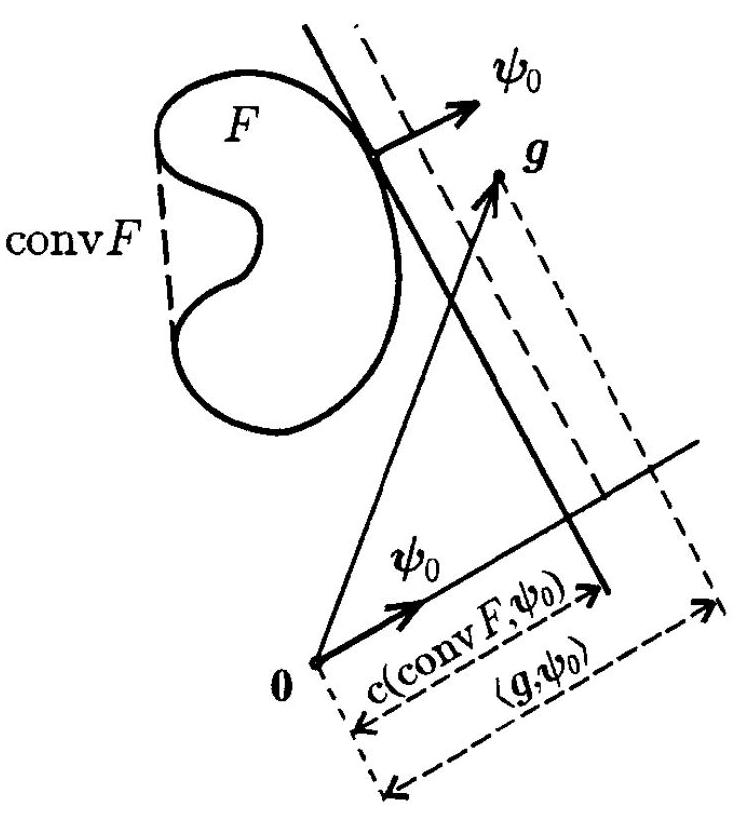
\includegraphics[max width=0.7\textwidth]{images/bo_d547okref24c73bgfch0_38_699_3_742_815_0.jpg}
\end{center}
\hspace*{3em} 

Рис. 9

Пусть теперь \(g \notin  \operatorname{conv}F\) . Множество conv \(F\) выпукло и компактно, и точка g ему не принадлежит. Тогда найдет- ся вектор \({\mathbf{\psi }}_{0} \in  S\) (puc. 9) ra- кой, что выполняется строгое HepaBeHCTBO

\[
c\left( {\operatorname{conv}F,{\psi }_{0}}\right)  < \left\langle  {\mathbf{g},{\psi }_{0}}\right\rangle  .
\]

B этом случае говорят, что гиперплоскость \({\Gamma }_{{\psi }_{\alpha }}\) cmporo отделяет точку g от множес- тва conv F. Геометрически этот факт представляется совершен- но очевидным, хотя и требует аккуратного аналитического до- казательства, которое приведено в разделе Д2 (см. дополнения). Из последнего неравенства согласно свойству 7 получаем

\[
c\left( {F,{\psi }_{0}}\right)  < \left\langle  {\mathbf{g},{\psi }_{0}}\right\rangle  .
\]

Таким образом, для данного вектора ф \({\psi }_{0} \in  S\) соответствую- щее полупространство в фигурных скобках в правой части соот- ношения (3.10) не содержит точки g. Тем более не содержит ее и пересечение всех этих полупространств, т.е. точка g не принад- лежит правой части соотношения (3.10). Свойство 8 доказано.

В дальнейшем, имея какие-либо соотношения для множеств, будем получать соответствующие соотношения для опорных функций. Обратно, из соотношений для опорных функций мож- но получать аналогичные соотношения лишь для выпуклых оболочек множеств. Это обстоятельство характерно проявля- ется в ряде свойств, приведенных ниже.

Свойство 9. Пусть F ∈ Ω(Ег’), f ∈ Е". Если для любого еекмора ψ ∈ S еыполияеmcя иеравенсмео

\[
\langle f,\psi \rangle  \leq  c\left( {F,\psi }\right) , \tag{3.11}
\]

то точка f принадлежит выпуклой оболочке conv F множес- тва F.

Доказательство. Пусть неравенство (3.11) выполняется для любого вектора \(\psi  \in  S\) . Тогда точка f принадлежит мно- жеству, стоящему в правой части соотношения (3.11). Следова- тельно, согласно свойству 8 имеем включение \(f \in  \operatorname{conv}F\) .

Следствие. Пусть множество F ∈ Ω(E") выпукло. В таком случае точка f принадлежит множеству F тогда и только тогда, когда выполняется неравенство (3.11) для лю- бого вектора ψ с \$ .

Для доказательства этого следствия достаточно воспользо- ваться свойством 9 и следствием свойства 6.

Заметим, что если множество \(F\) невыпукло, то из выполне- ния соотношения (3.11), вообще говоря, не следует, что f ∈ F.

Рассмотрим следующий пример.

Пример 7. Пусть множество F — единичная сфера в про- странстве \({E}^{n}\) , т.е. \(F = S\) , a \(f = 0\) . Тогда \(\langle f,\psi \rangle  = 0\) , a \(c\left( {F,\psi }\right)  = \parallel \psi \parallel\) . Таким образом, соотношение (3.11) выполняется, так как \(0 \leq  \parallel \psi \parallel\) ,но \(0 \notin  S\) .

Свойство 10. Пусть G, F ∈ Ω(E \({}^{n}\) ). Если для любого век- mopa \(\psi  \in  S\) esinonHAemca Hepasencmeo

\[
c\left( {G,\psi }\right)  \leq  c\left( {F,\psi }\right) , \tag{3.12}
\]

то справедливо включение \(G \subset  \operatorname{conv}F\) .

Доказательство. Предположим противное, т.е. G ⊄ \(\text{ ⊄ }\) conv \(F\) . Это означает, что существует точка \(g \in  G\) такая, что \(g \notin  \operatorname{conv}F\) . Множество conv \(F\) выпукло, поэтому согласно следствию из свойства 9 существует вектор \({\psi }_{0} \in  S\) такой,что

\[
\left\langle  {\mathbf{g},{\psi }_{0}}\right\rangle   > c\left( {\operatorname{conv}F,{\psi }_{0}}\right)  = c\left( {F,{\psi }_{0}}\right) .
\]

Из включения \(g \in  G\) ,пользуясь следствием из свойства 6, полу- чим неравенство

\[
\left\langle  {g,{\psi }_{0}}\right\rangle   \leq  c\left( {G,{\psi }_{0}}\right) .
\]

Издвух последних неравенств следует, что

\[
c\left( {G,{\psi }_{0}}\right)  > c\left( {F,{\psi }_{0}}\right)
\]

а это противоречит неравенству (3.12). Следовательно, свойст- во 10 доказано.

Замечание. Так как множество conv \(F\) выпукло, то из включения \(G \subset  \operatorname{conv}F\) следует включение conv \(G \subset  \operatorname{conv}F\) . По- этому если выполняется неравенство (3.12) для любого вектора \(\psi  \in  S\) , то справедливо включение conv \(G \subset  \operatorname{conv}F\) .

Следствие. Пусть G, F ∈ Ω(E \({}^{n}\) ) и множество F выпукло. Тогда включение G C F справедливо тогда и только тогда, когда для любого вектора ψ ∈ S выполняется неравенст- во (3.12).

Доказательство очевидным образом следует из свойств 10 и 6.

Свойство 11. Пусть \(G, F \in  \Omega \left( {E}^{n}\right)\) . Если множества \(F\) и \(G\) равны, т.е. \(F = G\) , то их опорные функции совпадают, \(c\left( {F,\psi }\right)  = c\left( {G,\psi }\right)\) . Наоборот, если опорные функции \(c\left( {F,\psi }\right)\) и \(c\left( {G,\psi }\right)\) совпадают, то conv \(F = \operatorname{conv}G\) .

Доказательство. Первое утверждение очевидным обра- зом следует из определения опорной функции (3.1), а второе — из свойства 10. Действительно, разбивая равенство \(c\left( {F,\psi }\right)  = \; = c\left( {G,\psi }\right)\) на два неравенства вида (3.12),получим два включе- ния

\[
G \subset  \operatorname{conv}F,\;F \subset  \operatorname{conv}G
\]

и, следовательно, равенство conv \(F = \operatorname{conv}G\) . Свойство 11 дока- зано.

Следствие. Выпуклые множества F, G € Ω(E’) равны тогда и только тогда, когда их опорные функции совпадают.

Это следствие будем в дальнейшем использовать для нахож- дения множества по опорной функции. Оно означает также, что выпуклое множество \(F \in  \Omega \left( {E}^{n}\right)\) можно однозначно восстано- вить по его опорной функции \(c\left( {F,\psi }\right)\) .

Таким образом, получаем взаимно однозначное соответствие между выпуклыми компактными множествами и их опорными функциями. При этом для любого свойства выпуклого множес- тва или совокупности выпуклых множеств имеется аналогич- ное свойство для опорных функций. Поэтому опорную функцию можно рассматривать как способ описания выпуклых множеств, который во многих случаях более предпочтителен. Например, выпуклое компактное множество достаточно сложного вида во- обще нереально ввести в ЭВМ из-за невозможности ввода всех точек этого множества. В то же время с разумной степенью точности можно в табличной форме ввести соответствующую опорную функцию и вместо множеств иметь дело с опорными функциями.

Далее, оказывается, что по виду произвольной функции \(c\left( \psi \right)  : {E}^{n} \rightarrow  {E}^{1}\) можно сразу сказать, будет она опорной к какому-либо множеству или нет. Если функция не принима- ет бесконечных значений и удовлетворяет свойствам 1 и 2, то она является опорной функцией некоторого множества F ∈ \(\in  \operatorname{conv}\Omega \left( {E}^{n}\right)\) , т.е. \(c\left( \psi \right)  = c\left( {F,\psi }\right)\) . При этом множество F легко восстанавливается по функции с(ф). Этот факт не будет ис- пользован при исследовании линейной задачи быстродействия, но он показывает эффективность применения опорных функций и аккуратно доказан в разделе Д4 (см. дополнения).

Понятие опорной функции можно ввести и исследовать со- ответствующие ее свойства и для неограниченных замкнутых выпуклых множеств [2]. Но это уже выходит за рамки данной книги.

Пример 8. Выпуклое множество \(F \in  \Omega \left( {E}^{n}\right)\) имеет опорную pynkiliton

\[
c\left( {F,\psi }\right)  = 5{\psi }^{1} + 2{\psi }^{2} + 3\parallel \psi \parallel .
\]

Как следует из примера 4, такую же опорную функцию име- ет map \({S}_{r}\left( a\right)\) c центром в точке a \(= \left( {5,2}\right)\) paдиуса \(r = 3\) . Таким образом, по следствию свойства 11 множество F совпадает с этим mapoм.

Пример 9. Докажем, что для любых двух множеств F, G ∈ \(\in  \Omega \left( {E}^{n}\right)\) , любой матрицы \(A\) размером \(n \times  n\) и любого числа \(\lambda\) выполняются равенства

\[
\operatorname{conv}\left( {F + G}\right)  = \operatorname{conv}F + \operatorname{conv}G,
\]

\[
\operatorname{conv}\left( {AF}\right)  = A\operatorname{conv}F
\]

\[
\operatorname{conv}\left( {\lambda F}\right)  = \lambda \operatorname{conv}F
\]

Множества в левой и правой частях этих соотношений яв- ляются выпуклыми, а их опорные функции совпадают согласно свойству 7 и свойствам 3, 4 и 5, соответственно. Следовательно, в силу следствия из свойства 11 эти множества также совпада- 10T.

Свойство 12. Пусть F, G ∈ Ω(En). Если множества F и G пересекаются, т.е. F ∩ G ≠ ∅, то для любого вектора ψ ∈ E" выполняется неравенство

\[
c\left( {F,\psi }\right)  + c\left( {G, - \psi }\right)  \geq  0. \tag{3.13}
\]

Наоборот, если выполняется соотношение (3.13) для любого вектора \(\psi  \in  S\) , \({mo}\) conv \(F \cap  \operatorname{conv}G \neq  \varnothing\) .

\[
0 \in  F + \left( {-1}\right) G\text{ . } \tag{3.1}
\]

Действительно, пусть \(F \cap  G \neq  \varnothing\) и \(x \in  F \cap  G\) . Тогда \(x \in \; \mathbf{u}\mathbf{x} \in  G\) , т.е. \(- \mathbf{x} \in  \left( {-1}\right) G\) . Таким образом, \(\mathbf{0} = \mathbf{x} + \left( {-\mathbf{x}}\right)  \in  F\) , \(+ \left( {-1}\right) G\) . Наоборот, пусть 0 \(\in  F + \left( {-1}\right) G\) . Тогда по определени и суммы множеств 0 = \(f + \left( {-1}\right) g\) ,где \(f \in  F,g \in  G\) . Take 1 образом, \(f \in  F\) и \(g \in  G\) ,т.е. \(F \cap  G \neq  \varnothing\) .

Пусть теперь \(F,G \in  \Omega \left( {E}^{n}\right)\) и \(F \cap  G \neq  \varnothing\) . Применяя к соотн з шению (3.13) следствие из свойства 6, получим

\[
0 = \langle \mathbf{0},\psi \rangle  \leq  c\left( {F + \left( {-1}\right) G,\psi }\right) .
\]

Откуда согласно свойствам Зи 5 следует неравенство

\[
0 \leq  c\left( {F,\psi }\right)  + c\left( {G, - \psi }\right)
\]

т.е. соотношение (3.13) выполнено.

Пусть теперь выполняется соотношение (3.13). Тогда с : гласно свойствам 3 и 5 имеем

\[
c\left( {F + \left( {-1}\right) G,\psi }\right)  = c\left( {F,\psi }\right)  + c\left( {G, - \psi }\right)  \geq  0.
\]

Откуда,используя свойство 9,находим

\[
0 \in  \operatorname{conv}\left( {F + \left( {-1}\right) G}\right)  = \operatorname{conv}F + \left( {-1}\right) \operatorname{conv}G.
\]

В результате согласно формуле (3.14) имеем conv \(F \cap\) conv \(G \neq  \varnothing\)

Таким образом, свойство 12 доказано полностью.

Следствие. Два выпуклых множества F, G ∈ Ω(Er) пересекаются тогда и только тогда, когда неравенство

\[
c\left( {F,\psi }\right)  + c\left( {G, - \psi }\right)  \geq  0
\]

выполняется для любого вектора ψ ∈ S.

Свойство 13. Опорная функция с(F, ψ) для любых дву множеств F, \({F}_{0} \in  \Omega \left( {E}^{n}\right) u\) любых двух векторов \(\psi ,{\psi }_{0} \in  E\) удовлетворяет неравенству

\[
\left| {c\left( {F,\psi }\right)  - c\left( {{F}_{0},{\psi }_{0}}\right) }\right|  \leq  \left\lVert \begin{array}{c} {\psi }_{0} \end{array} \right\rVert h\left( {F,{F}_{0}}\right)  + \left\lVert \begin{array}{c} {F}_{0} \end{array} \right\rVert \cdot  \left\lVert \begin{array}{c} {\psi  - {\psi }_{0}} \end{array} \right\rVert +
\]

\[
+ {2h}\left( {F,{F}_{0}}\right) \left\lVert \begin{array}{c} {\psi  - {\psi }_{0}} \end{array} \right\rVert. \tag{3.18}
\]

Доказательство. Пусть F, \({F}_{0} \in  \Omega \left( {E}^{n}\right)\) — два произволь- ных множества, а 秒, му — два произвольных вектора из про- странства E". Из свойства 2 опорных функций следует неравен- CTBO

\[
c\left( {F,\psi }\right)  = c\left( {F,\psi  - {\psi }_{0} + {\psi }_{0}}\right)  \leq  c\left( {F,\psi  - {\psi }_{0}}\right)  + c\left( {F,{\psi }_{0}}\right) . \tag{3.16}
\]

По определению модуля множества |F| и хаусдорфова расстоя- ния \(h\left( {F,{F}_{0}}\right)\) (см. лекцию 2) справедливы включения

\[
F \subset  {S}_{\left| F\right| }\left( \mathbf{0}\right) ,\;F \subset  {F}_{0} + {S}_{h\left( {F,{F}_{0}}\right) }\left( \mathbf{0}\right) .
\]

Применяя свойство 6 к этим включениям для векторов ψ — \({\psi }_{0}\) и \({\psi }_{0}\) coответственно, получаем неравенства

\[
c\left( {F,\psi  - {\psi }_{0}}\right)  \leq  \left| F\right|  \cdot  \parallel \psi  - {\psi }_{0}\parallel ,\;c\left( {F,{\psi }_{0}}\right)  \leq  c\left( {{F}_{0},{\psi }_{0}}\right)  + h\left( {F,{F}_{0}}\right) \left\lVert \begin{array}{c} {\psi }_{0} \end{array} \right\rVert.
\]

Подставляя эти неравенства в неравенство (3.16) и перенося \(\mathrm{c}\left( {{F}_{0},{\psi }_{0}}\right)\) в левую часть, получаем соотношение

\[
c\left( {F,\psi }\right)  - c\left( {{F}_{0},{\psi }_{0}}\right)  \leq  \left| F\right|  \cdot  \left\lVert \begin{array}{c} {\psi  - {\psi }_{0}} \end{array} \right\rVert + h\left( {F,{F}_{0}}\right) \left\lVert \begin{array}{c} {\psi }_{0} \end{array} \right\rVert.
\]

Поскольку множества F, F0 и векторы ψ, ф, произвольны, пере- мена их местами не изменяет полученного неравенства. Таким образом, имеем также неравенство

\[
c\left( {{F}_{0},{\mathbf{\psi }}_{0}}\right)  - c\left( {F,\mathbf{\psi }}\right)  \leq  \left| {F}_{0}\right|  \cdot  \left\lVert \begin{array}{c} {{\mathbf{\psi }}_{0} - \mathbf{\psi }} \end{array} \right\rVert + h\left( {{F}_{0},F}\right) \parallel \mathbf{\psi }\parallel .
\]

Издвух последних неравенств следует соотношение

\[
\left| {c\left( {F,\psi }\right)  - c\left( {{F}_{0},{\psi }_{0}}\right) }\right|  \leq  \left\lVert \begin{array}{c} {\psi  - {\psi }_{0}} \end{array} \right\rVert\max \left( {\left| F\right| ,\left| {F}_{0}\right| }\right)  +
\]

\[
+ h\left( {F,{F}_{0}}\right) \max \left( {\parallel \mathbf{\psi }\parallel ,\left\lVert \begin{array}{c} {\mathbf{\psi }}_{0} \end{array} \right\rVert}\right) .
\]

Оценим в этом соотношении \(\parallel \mathbf{\psi }\parallel\) и \(\left| F\right|\) следующими величина- ми:

\[
\parallel \mathbf{\psi }\parallel  = \left\lVert \begin{array}{c} {\mathbf{\psi } - {\mathbf{\psi }}_{0} + {\mathbf{\psi }}_{0}} \end{array} \right\rVert \leq  \left\lVert \begin{array}{c} {\mathbf{\psi } - {\mathbf{\psi }}_{0}} \end{array} \right\rVert + \left\lVert \begin{array}{c} {\mathbf{\psi }}_{0} \end{array} \right\rVert,
\]

\[
\left| F\right|  = h\left( {F,\{ 0\} }\right)  \leq  h\left( {F,{F}_{0}}\right)  + h\left( {F,\{ 0\} }\right)  = h\left( {F,{F}_{0}}\right)  + \left| {F}_{0}\right| .
\]

Тогда имеем неравенства

\[
\max \left( {\parallel \mathbf{\psi }\parallel ,\left\lVert \begin{array}{c} {\mathbf{\psi }}_{0} \end{array} \right\rVert}\right)  \leq  \left\lVert \begin{array}{c} {\mathbf{\psi }}_{0} \end{array} \right\rVert + \left\lVert \begin{array}{c} {\mathbf{\psi } - {\mathbf{\psi }}_{0}} \end{array} \right\rVert,
\]

\[
\max \left( {\left| F\right| ,\left| {F}_{0}\right| }\right)  \leq  \left| {F}_{0}\right|  + h\left( {F,{F}_{0}}\right) .
\]

Подставляя их в неравенство (3.16), получаем нужное неравен- ство (3.15). Тем самым свойство 13 доказано.

Из этого свойства сразу следует непрерывность опорной функции \(c\left( {F,\psi }\right)\) .

Непрерывность опорной функции \(c\left( {F, \cdot  }\right)  : {E}^{n} \rightarrow  {E}^{1}\) по пере- менной \(\mathbf{\psi }\) в точке \({\mathbf{\psi }}_{0} \in  {E}^{n}\) означает,что если точка ψ стремится к точке ф, то значение функции \(c\left( {F,\psi }\right)\) стремится к значению \(c\left( {F,{\psi }_{0}}\right)\) . Таким образом, для любого числа ε > 0 существует число \(\delta  > 0\) такое,что при \(\left\lVert \begin{array}{c} {\psi  - {\psi }_{0}} \end{array} \right\rVert \leq  \delta\) выполняется неравен- CTBO

\[
\left| {c\left( {F,\psi }\right)  - c\left( {F,{\psi }_{0}}\right) }\right|  \leq  \varepsilon .
\]

Непрерывность опорной функции \(c\left( {\cdot ,\psi }\right)  : \Omega \left( {E}^{n}\right)  \rightarrow  {E}^{1}\) no переменной \(F\) в точке \({F}_{0} \in  \Omega \left( {E}^{n}\right)\) означает,что если точка \(F\) стремится к точке \({F}_{0}\) , то значение \(c\left( {F,\psi }\right)\) стремится к значению \(c\left( {{F}_{0},\psi }\right)\) . Таким образом, для любого числа ε > 0 существует число \(\delta  > 0\) такое,что при \(h\left( {F,{F}_{0}}\right)  \leq  \delta\) выполняется неравенст- BO

\[
\left| {c\left( {F,\psi }\right)  - c\left( {{F}_{0},\psi }\right) }\right|  \leq  \varepsilon
\]

Непрерывность опорной функции \(c\left( {F,\mathbf{\psi }}\right)\) по совокупности пе- ременных \(F,\mathbf{\psi }\) в точке \(\left( {{F}_{0},{\mathbf{\psi }}_{0}}\right)\) означает,что если F стремится к \({F}_{0}\) и одновременно \(\mathbf{\psi }\) стремится к \({\mathbf{\psi }}_{0}\) , то значение с \(\left( {F,\mathbf{\psi }}\right)\) стре- мится к значению \(c\left( {{F}_{0},{\mathbf{\psi }}_{0}}\right)\) . Таким образом, для любого числа \(\varepsilon  > 0\) cyществует такое число \(\delta  > 0\) ,что при

\[
h\left( {F,{F}_{0}}\right)  \leq  \delta ,\;\left\lVert \begin{array}{c} {\psi  - {\psi }_{0}} \end{array} \right\rVert \leq  \delta
\]

выполняется неравенство

\[
\left| {c\left( {F,\psi }\right)  - c\left( {{F}_{0},{\psi }_{0}}\right) }\right|  \leq  \varepsilon
\]

Из выражения (3.15) следует, что последнее неравенство будет выполнено, если по заданному числу ε > 0 выбрать число δ > 0, удовлетворяющее соотношению

\[
\left\lVert \begin{array}{c} {\psi }_{0} \end{array} \right\rVert\delta  + \left| {F}_{0}\right| \delta  + 2{\delta }^{2} \leq  \varepsilon .
\]

Таким образом, мы доказали следующее следствие из свой- ства 13.

Следствие. Опорная функция \(c\left( {F,\psi }\right)\) непрерывна по сово- купности переменных \(F,\psi\) в любой точке \(\left( {{F}_{0},{\psi }_{0}}\right) u,c\) ледова- тельно, непрерывна по каждой из переменных F и ψ в отдель- ности.

Свойство 14. Пусть F ∈ \(\Omega \left( {E}^{n}\right)\) . Ecau moчка f являет- ся внутренней точкой множества F, т.е. f ∈ int F, то для любого вектора ψ с ∈ S выполняется неравенство

\[
\langle \mathbf{f},\psi \rangle  < c\left( {F,\psi }\right) . \tag{3.17}
\]

Наоборот, если соотношение (3.17) выполняется для любого вектора \(\psi  \in  S\) , mo \(f \in  \operatorname{int}\operatorname{conv}F\) .

Доказательство. Пусть f ∈ int F. Тогда существует чис- ло \(\varepsilon  > 0\) такое,что \({S}_{\varepsilon }\left( \mathbf{f}\right)  \subset  F\) . Oткуда согласно свойству 6 следует, что неравенство

\[
\mathrm{c}\left( {{S}_{\varepsilon }\left( \mathbf{f}\right) ,\psi }\right)  \leq  c\left( {F,\psi }\right)
\]

выполняется для любого вектора ψ с S . Подставив в полу- ченное неравенство выражение опорной функции шара \({S}_{\varepsilon }\left( \mathbf{f}\right)\) , приходим к неравенству

\[
\langle \mathbf{f},\mathbf{\psi }\rangle  + \varepsilon \parallel \mathbf{\psi }\parallel  \leq  c\left( {F,\mathbf{\psi }}\right) .
\]

Поэтому соотношение (3.17) верно для всех векторов ψ с S. Пусть теперь неравенство (3.17) выполняется для любого век- тора ψ ∈ S. Поскольку опорная функция \(c\left( {F,\mathbf{\psi }}\right)\) непрерывна по \(\mathbf{\psi }\) (следствие из свойства 13), то функция \(c\left( {F,\mathbf{\psi }}\right)  - \langle \mathbf{f},\mathbf{\psi }\rangle\) непрерывна по \(\mathbf{\psi }\) и положительна для всех векторов \(\mathbf{\psi } \in  S\) . Минимум этой непрерывной функции на компактном множестве \(S\) достигается и положителен. Обозначим его через ε. Таким образом, неравенство

\[
c\left( {F,\psi }\right)  - \langle f,\psi \rangle  \geq  \varepsilon  > 0
\]

справедливо для всех векторов \(\psi  \in  S\) ,т.е.

\[
\langle \mathbf{f},\mathbf{\psi }\rangle  + \varepsilon \parallel \mathbf{\psi }\parallel  \leq  c\left( {F,\mathbf{\psi }}\right) .
\]

Перепишем это неравенство В виде

\[
c\left( {{S}_{\varepsilon }\left( \mathbf{f}\right) ,\psi }\right)  \leq  c\left( {F,\psi }\right) .
\]

\(\left( {\mu ,r}\right)\)

Corracho свойству 10 отсюда следует включение \({S}_{\varepsilon }\left( \mathbf{f}\right)  \subset  F\) . Это и означает, что f является внутренней точкой множества conv \(F\) .

Следствие. Точка f принадлежит внутренности выпук- лого множества F ∈ Ω(E") тогда и только тогда, когда не- paseксмео (3.17) справеòлиео dnд любоzo еекмора ψ \(\in  S\) .

\[
d - a{v}^{p} : {S}_{5}\left( f\right)  \subset  \operatorname{conv}F
\]

Свойство 15. Пусть заданы два множества F, G ∈ Ω(E \({}^{n}\) ). Тогда справедливо соотношение

\[
h\left( {\operatorname{conv}F,\operatorname{conv}G}\right)  = \mathop{\max }\limits_{{\psi  \in  S}}\left| {c\left( {F,\psi }\right)  - c\left( {G,\psi }\right) }\right|  \leq  h\left( {F,G}\right) . \tag{3.18}
\]

Доказательство. Неравенство в этом соотношении непо- средственно следует из свойства 13. Действительно, для любого вектора ф \(\in  S\) имеем

\[
\left| {c\left( {F,\psi }\right)  - c\left( {G,\psi }\right) }\right|  \leq  h\left( {F,G}\right) ,
\]

следовательно, справедливо неравенство

\[
\mathop{\max }\limits_{{\psi  \in  S}}\left| {c\left( {F,\psi }\right)  - c\left( {G,\psi }\right) }\right|  \leq  h\left( {F,G}\right) .
\]

Хаусдорфово расстояние определяется выражением

\[
h\left( {\operatorname{conv}F,\operatorname{conv}G}\right)  = \min \{ r \geq  0 : \operatorname{conv}F \subset  \operatorname{conv}G + {S}_{r}\left( \mathbf{0}\right) ,
\]

\[
\left. {\operatorname{conv}F \subset  \operatorname{conv}G + {S}_{r}\left( \mathbf{0}\right) }\right\}
\]

Множества conv \(F\) , conv \(G\) выпуклы и их опорные функции \(c\left( {\operatorname{conv}F,\mathbf{\psi }}\right) ,c\left( {\operatorname{conv}G,\mathbf{\psi }}\right)\) cosnaдают c \(c\left( {F,\mathbf{\psi }}\right) ,c\left( {G,\mathbf{\psi }}\right)\) в силу свойства 7, поэтому включения в фигурных скобках можно запи- сать в эквивалентной форме в виде неравенств. Согласно след- ствию из свойства 10 имеем

\[
h\left( {\operatorname{conv}F,\operatorname{conv}G}\right)  = \min \{ r \geq  0 : c\left( {F,\psi }\right)  \leq  c\left( {G,\psi }\right)  + r
\]

\[
c\left( {G,\psi }\right)  \leq  c\left( {F,\psi }\right)  + r,\psi  \in  S\}  =
\]

\[
= \min \left\{  {r \geq  0 : \left| {c\left( {F,\psi }\right)  - c\left( {G,\psi }\right) }\right|  \leq  r,\psi  \in  S}\right\}   =
\]

\[
= \mathop{\max }\limits_{{\psi  \in  S}}\left| {c\left( {F,\psi }\right)  - c\left( {G,\psi }\right) }\right| .
\]

Следовательно, свойство 15 доказано.

Следствие. Для выпуклых множеств F, G ∈ Ω(En) спра- ведливо равенство

\[
h\left( {F,G}\right)  = \mathop{\max }\limits_{{\psi  \in  S}}\left| {c\left( {F,\psi }\right)  - c\left( {G,\psi }\right) }\right| . \tag{3.19}
\]

Заметим, что если множества F и G не являются выпук- лыми, то в формуле (3.18) может быть строгое неравенство. Приведем пример.

\begin{center}
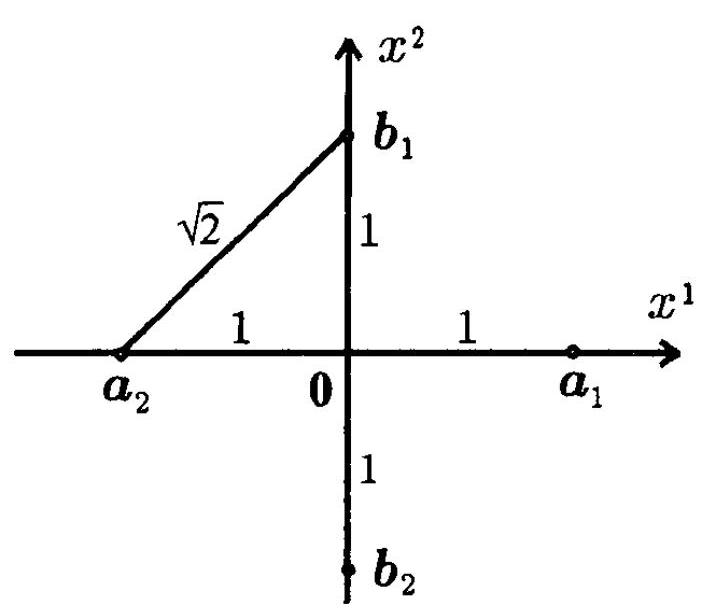
\includegraphics[max width=0.6\textwidth]{images/bo_d547okref24c73bgfch0_47_0_12_703_614_0.jpg}
\end{center}
\hspace*{3em} 

Рис. 10

Пример 10. Пусть \(n = 2\) , множество F состоит из двух точек а \({a}_{1} = \left( {1,0}\right)\) и \({a}_{2} = \left( {-1,0}\right)\) , a множест- во \(G\) coconut из двух точек \({b}_{1} = \left( {0,1}\right)\) и \({b}_{2} = \left( {0, - 1}\right)\) (рис. 10). Тогда непосред- ственно можно проверить, что \(h\left( {F,G}\right)  = \sqrt{2}\) . C дру- roй стороны, \(c\left( {F,\psi }\right)  = \left| {\psi }^{1}\right|\) , \(c\left( {G,\psi }\right)  = \left| {\psi }^{2}\right|\) . Таким обра- 30M,

\[
\mathop{\max }\limits_{{\psi  \in  S}}\left| {c\left( {F,\psi }\right)  - c\left( {G,\psi }\right) }\right|  = \mathop{\max }\limits_{{\psi  \in  S}}\left| \right| {\psi }^{1}\left| -\right| {\psi }^{2}\left| \right| \; = 1 < \sqrt{2} = h\left( {F,G}\right) .
\]

Cледующий пример показывает, как, используя формулу (3.19), найти хаусдорфово расстояние между множествами.

Пример 11. Найдем хаусдорфово расстояние между произ- вольными шарами \({S}_{{r}_{1}}\left( {a}_{1}\right)\) и \({S}_{{r}_{2}}\left( {a}_{2}\right)\) . Воспользовавшись форму- лой (3.19), имеем равенства

\[
h\left( {{S}_{{r}_{1}}\left( {a}_{1}\right) ,{S}_{{r}_{2}}\left( {a}_{2}\right) }\right)  = \mathop{\max }\limits_{{\psi  \in  S}}\left| {\left\langle  {{a}_{1},\psi }\right\rangle   + {r}_{1}\parallel \psi \parallel  - \left\langle  {{a}_{2},\psi }\right\rangle   - {r}_{2}\parallel \psi \parallel }\right|  =
\]

\[
= \mathop{\max }\limits_{{\psi  \in  S}}\left| {\left\langle  {{\mathbf{a}}_{1} - {\mathbf{a}}_{2},\psi }\right\rangle   + {r}_{1} - {r}_{2}}\right| .
\]

Нетрудно показать, что максимум в последнем выражении до- стигается на векторе

\[
\psi  = \operatorname{sign}\left( {{r}_{1} - {r}_{2}}\right) \frac{{a}_{1} - {a}_{2}}{\left\lVert \begin{array}{c} {a}_{1} - {a}_{2} \end{array} \right\rVert} \in  S,
\]

если \({a}_{1} \neq  {a}_{2}\) ,и на любом векторе фе S, ecли \({a}_{1} = {a}_{2}\) . Таким образом, окончательно имеем формулу

\[
h\left( {{S}_{{r}_{1}}\left( {\mathbf{a}}_{1}\right) ,{S}_{{r}_{2}}\left( {\mathbf{a}}_{2}\right) }\right)  = \left\lVert \begin{array}{c} {{\mathbf{a}}_{1} - {\mathbf{a}}_{2}} \end{array} \right\rVert + \left| {{\mathbf{r}}_{1} - {\mathbf{r}}_{2}}\right| .
\]

\section*{3.5. Задачи}

1. Haйдите опорную функцию n-мерного куба

\[
F = \left\{  {\mathbf{x} \in  {E}^{n} : \left| {x}^{i}\right|  \leq  1,i = 1,\ldots ,n}\right\}  .
\]

2. Найдите опорную функцию произвольного n-мерного па- раллелепипеда G с ребрами, параллельными осям координат,

\[
G = \left\{  {\mathbf{x} \in  {E}^{n} : {a}^{i} \leq  {x}^{i} \leq  {b}^{i},i = 1,\ldots ,n}\right\}  .
\]

3. Найдите опорную функцию множества F, заданного на плоскости формулой

\[
F = \left\{  {\mathbf{x} \in  {E}^{2} : \left| {{x}^{1} + {x}^{2}}\right|  \leq  1,\left| {{x}^{1} - {x}^{2}}\right|  \leq  1}\right\}  .
\]

4. Найдите опорную функцию эллипса, заданного на плос- кости \({E}^{2}\) уравнением

\[
{\left( \frac{{x}^{1}}{a}\right) }^{2} + {\left( \frac{{x}^{2}}{b}\right) }^{2} = 1,\;a,b \neq  0.
\]

5. Haйдите опорную функцию множества

\[
F = \left\{  {x \in  {E}^{2} : {\left( \frac{{x}^{1} - a}{c}\right) }^{2} + {\left( \frac{{x}^{2} - b}{d}\right) }^{2} \leq  1}\right\}  ,\;c,d \neq  0.
\]

6. Haйдите опорную функцию множества

\[
F = \left\{  {\mathbf{x} \in  {E}^{2} : \langle A\mathbf{x},\mathbf{x}\rangle  \leq  1}\right\}  ,
\]

где A — симметричная положительно определенная матрица размером \(2 \times  2\) .

7*. Найдите опорную функцию множества

\[
F = \left\{  {x \in  {E}^{2} : {\left| \frac{{x}^{1}}{a}\right| }^{p} + {\left| \frac{{x}^{2}}{b}\right| }^{p} \leq  1}\right\}  ,\;a,b \neq  0,
\]

где \(p -\) некоторое число, \(p > 1\) .

8. Найдите опорную функцию множества

\[
F = {S}_{2}\left( \left( {0,2}\right) \right)  \cup  {S}_{2}\left( \left( {0, - 2}\right) \right) .
\]

9.Найдите опорную функцию n-мерного эллипсоида

\[
F = \left\{  {\mathbf{x} \in  {E}^{n} : \mathop{\sum }\limits_{{i = 1}}^{n}{\left( \frac{{x}^{i}}{{a}^{i}}\right) }^{2} \leq  1}\right\}  ,\;{a}^{i} \neq  0.
\]

10. Восстановите множество \(F \in  \Omega \left( {E}^{2}\right)\) по его опорной функ- ции

\[
c\left( {F,\psi }\right)  = \left| {{\psi }^{1} - {\psi }^{2}}\right| .
\]

11. Найдите с помощью свойства 12 условия, при которых два произвольных шара \({S}_{{r}_{1}}\left( {a}_{1}\right)\) и \({S}_{{r}_{2}}\left( {a}_{2}\right)\) имеют непустое пере- сечение.

12. Найдите опорную функцию объединения двух множеств \(F \cup  G\) .

13*. Найдите опорную функцию пересечения двух множеств \(F \cap  G\) .

\({14}^{ * }\) . Размерностью множества F € Ω(En) назовем раз- мерность минимального линейного многообразия, содержащего множество \(F\) . Найдите размерность множества F с помощью его опорной функции \(c\left( {F,\psi }\right)\) .

15. Найдите радиус минимального шара, содержащего мно- жество \(F\) .

16. Найдите радиус максимального шара, вписанного в вы- пуклое множество F.

17. Диаметром множества F называется число

\[
d\left( F\right)  = \mathop{\max }\limits_{{{f}_{1},{f}_{2} \in  F}}\left\lVert \begin{array}{c} {{f}_{1} - {f}_{2}} \end{array} \right\rVert.
\]

Найдите диаметр множества F через его опорную функцию \(c\left( {F,\psi }\right)\) .

18. Евклидово расстояние между множествами F и G опре- деляется формулой

\[
\rho \left( {F,G}\right)  = \mathop{\min }\limits_{{f \in  F,g \in  G}}\parallel f - g\parallel .
\]

Найдите евклидово расстояние ρ(F, G) между выпуклыми мно- жествами \(F,G \in  \Omega \left( {E}^{n}\right)\) через их опорные функции.

19. Найдите евклидово расстояние \(\rho \left( {\mathbf{p},G}\right)\) от точки p ∈ \({E}^{n}\) до выпуклого множества F = Ω(Er).

20. Докажите, что для любых точек p, q ∈ \({E}^{n}\) и любых множеств \(F,G \in  \Omega \left( {E}^{n}\right)\) выполняются неравенства

\[
\rho \left( {\mathbf{p},F}\right)  \leq  \parallel \mathbf{p} - \mathbf{q}\parallel  + \rho \left( {\mathbf{q},F}\right) ,\;\rho \left( {\mathbf{p},F}\right)  \leq  \rho \left( {\mathbf{p},G}\right)  + h\left( {G,F}\right) .
\]

21. Докажите, что для любого множества F ∈ \(\Omega \left( {E}^{n}\right)\) и лю- бого вектора ф \(\in  S\) выполняется неравенство

\[
\left| {c\left( {F,\psi }\right) }\right|  \leq  \left| F\right|  \cdot  \parallel \psi \parallel .
\]

22. Выразите модуль |F| множества F через опорную функ- цию \(c\left( {F,\psi }\right)\) .

\section*{JIEKIJIN 4}

\begin{itemize}\relax
\item\relax Измеримые функции.
\end{itemize}

\begin{itemize}\relax
\item\relax Многозначные отображения.
\end{itemize}

\begin{itemize}\relax
\item\relax Свойства непрерывных многозначных отображений.
\end{itemize}

\begin{itemize}\relax
\item\relax Непрерывные и измеримые однозначные ветви мно- гозначных отображений.
\end{itemize}

\section*{4.1. Измеримые функции}

До сих пор мы имели дело лишь с классом непрерыв- ных функций. Однако в математической теории оптимального управления приходится рассматривать более широкий класс функций. Отчасти это объясняется незамкнутостью простран- ства непрерывных функций относительно поточечной сходи- мости, т.е. тем обстоятельством, что поточечный предел по- следовательности непрерывных функций может уже не быть непрерывной функцией. Поясним это на примере.

Пример 1. Рассмотрим последовательность непрерывных функций \({f}_{k} : {E}^{1} \rightarrow  {E}^{1}\) , onpeделенных на отрезке времени [0, \({t}^{ * }\) ] следующими условиями

\[
{f}_{k}\left( t\right)  = \left\{  \begin{array}{ll}  + 1, & \operatorname{ec\text{ л }\text{ и }}0 \leq  t \leq  \frac{{t}^{ * }}{2}, \\   - \frac{{2}^{k + 1}}{{t}^{ * }}t + {2}^{k} + 1, & \operatorname{ec\text{ л }\text{ и }}\frac{{t}^{ * }}{2} < t \leq  \left( {\frac{1}{2} + \frac{1}{{2}^{k}}}\right) {t}^{ * }, \\   - 1, & \operatorname{ec\text{ л }\text{ и }}\left( {\frac{1}{2} + \frac{1}{{2}^{k}}}\right) {t}^{ * } < t \leq  {t}^{ * }. \end{array}\right.
\]

Графики этих функций изображены на рис. 11.

Ясно, что для любого \(t \in  \left\lbrack  {0,{t}^{ * }}\right\rbrack\) последовательность \({f}_{k}\left( t\right)\) сходится к некоторому значению \(f\left( t\right)\) . Эта предельная функция \(f\left( t\right)\) yxe не непрерывна, a имеет разрыв при \(t = \frac{{t}^{ * }}{2}\) . Функция \(f\left( t\right)\) onpeдenяeтся соотношением

\[
f\left( t\right)  = \left\{  \begin{array}{ll}  + 1, & \operatorname{\text{ е }\text{ с }\text{ л }\text{ и }}0 \leq  t \leq  \frac{{t}^{ * }}{2}, \\   - 1, & \operatorname{\text{ е }\text{ с }\text{ л }\text{ и }}\frac{{t}^{ * }}{2} < t \leq  {t}^{ * }. \end{array}\right. \tag{4.1}
\]

\begin{center}
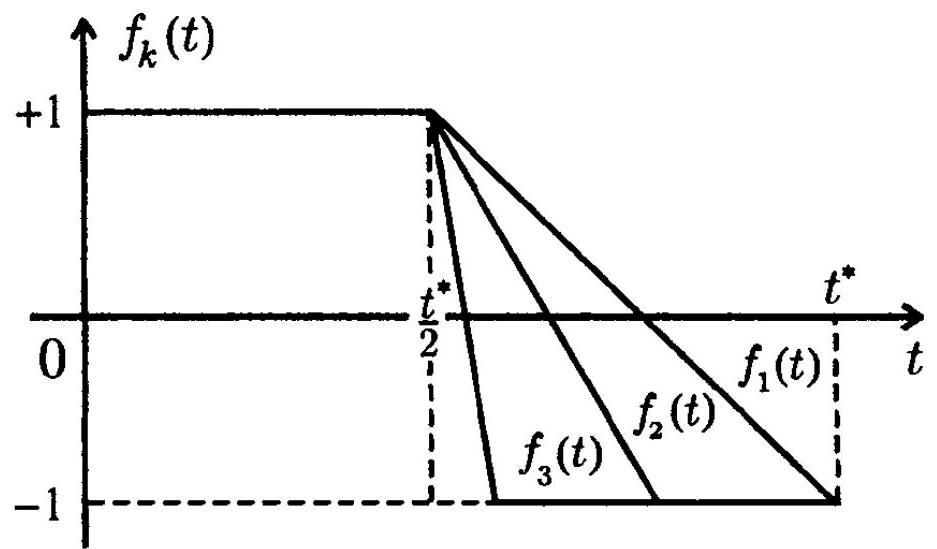
\includegraphics[max width=0.9\textwidth]{images/bo_d547okref24c73bgfch0_51_260_0_937_549_0.jpg}
\end{center}
\hspace*{3em} 

Рис. 11

Таким образом, поточечный предел последовательности не- прерывных функций уже может быть функцией разрывной. Же- лательно ввести такое пространство функций, чтобы предел любой последовательности функций этого пространства также ему принадлежал.

Покажем на примере, почему в теории оптимального управ- ления не удается обойтись классом непрерывных функций. Ока- зывается, что даже в простейших задачах оптимального управ- ления функция управления и(t) может оказаться разрывной.

Пример 2. Рассмотрим поезд, движущийся от станции A к станции \(B\) в соответствии с уравнением

\[
\ddot{x} = u,
\]

где х — расстояние от станции А до поезда; и — тяга поезда, которой можно управлять, т. е. выбирать ее как функцию време- ни \(u\left( t\right)\) . На величину тяги \(u\left( t\right)\) наложено ограничение \(\left| {u\left( t\right) }\right|  \leq  1\) . Расстояние между станциями А и В задано. Требуется так выбирать управление и(t), чтобы поезд преодолел путь между станциями за наименьшее время t*. При этом, конечно, имеется в виду, что скорость поезда в начальный и конечный моменты времени должна быть нулевой, т.е. \(\dot{x}\left( 0\right)  = \dot{x}\left( {t}^{ * }\right)  = 0\) .

Нетрудно сообразить, что время перехода будет минималь- ным, когда поезд до половины пути разгоняется с максималь- ным ускорением, т.е. и(t) = +1, а вторую половину пути мак- симально затормаживается, т.е. и \(u\left( t\right)  =  - 1\) . Таким образом, оп- тимальное управление \({u}^{ * }\left( t\right)\) вданном случае имеет вид

\[
{u}^{ * }\left( t\right)  = \left\{  \begin{array}{ll}  + 1, & \operatorname{\text{ е }\text{ с }\text{ л }\text{ и }}0 \leq  t \leq  \frac{{t}^{ * }}{2}, \\   - 1, & \operatorname{\text{ е }\text{ с }\text{ л }\text{ и }}\frac{{t}^{ * }}{2} < t \leq  {t}^{ * }, \end{array}\right.
\]

т.е. является функцией разрывной. Эта функция \({u}^{ * }\left( t\right)\) совпадает c функцией \(f\left( t\right)\) из примера 1 (см. формулу (4.1)), которая была получена как предел последовательности непрерывных функ- ций.

Таким образом, оптимальное управление и*(t) в примере 2 оказалось функцией не непрерывной, а разрывной. Более ши- роким классом функций является класс кусочно непрерывных функций \(D\) .

Функция \(f : {E}^{1} \rightarrow  {E}^{n}\) называется кусочно непрерывной на отрезке времени \(\left\lbrack  {{t}_{0},{t}_{1}}\right\rbrack\) , если она непрерывна во всех точках этого отрезка, кроме конечного числа точек \({\tau }_{1},\ldots ,{\tau }_{k}\) , а в этих точках существуют конечные пределы функции \(\mathbf{f}\left( t\right)\) и слева и справа. Если \(C\) — класс всех непрерывных функций, то ясно, что \(C \subset  D\) .

Оптимальное управление \({u}^{ * }\left( t\right)\) в примере 2 является кусочно непрерывной функцией на отрезке времени [0, 1] с одной точкой разрыва \(\tau  = \frac{1}{2}\) . Однако даже в линейной задаче быстродейст- вия (см. лекцию 1) оптимальное управление и*(t) может иметь счетное число точек разрыва. Более того, множество точек раз- рыва может быть еще более сложного вида. В общем случае оптимальное управление является функцией измеримой.

Функция \(f : {E}^{1} \rightarrow  {E}^{n}\) называется измеримой на отрезке \(\left\lbrack  {{t}_{0},{t}_{1}}\right\rbrack\) , если она является поточечным пределом некоторой после- довательности \({\mathbf{f}}_{k}\left( t\right)\) непрерывных функций, т.е. если при всех \(t \in  \left\lbrack  {{t}_{0},{t}_{1}}\right\rbrack\) выполняется соотношение

\[
f\left( t\right)  = \mathop{\lim }\limits_{{k \rightarrow  \infty }}{f}_{k}\left( t\right)
\]

Если L — класс всех измеримых функций, то, очевидно, справедливы включения \(C \subset  D \subset  L\) .

Приведенное определение измеримой функции не является общепринятым в математическом анализе. Обычно оно дается другим способом и опирается на понятие измеримого множест- ва. Использованное нами в качестве определения соотношение служит при этом критерием измеримости. Читателям, желаю- щим ознакомиться с этими понятиями, рекомендуется прочи- тать раздел Д6 (см. дополнения), где даны аккуратные опреде- ления и приведены те свойства измеримых функций, которые необходимы для строгого построения математической теории оптимального управления. Однако при первом знакомстве с те- орией оптимального управления этот материал можно пропус- тить и, встречая в тексте слова “измеримая функция”, представ- лять себе, что имеете дело с кусочно непрерывной функцией. При этом не все теоремы будут справедливы (соответствующие замечания в книге даны).

\begin{center}
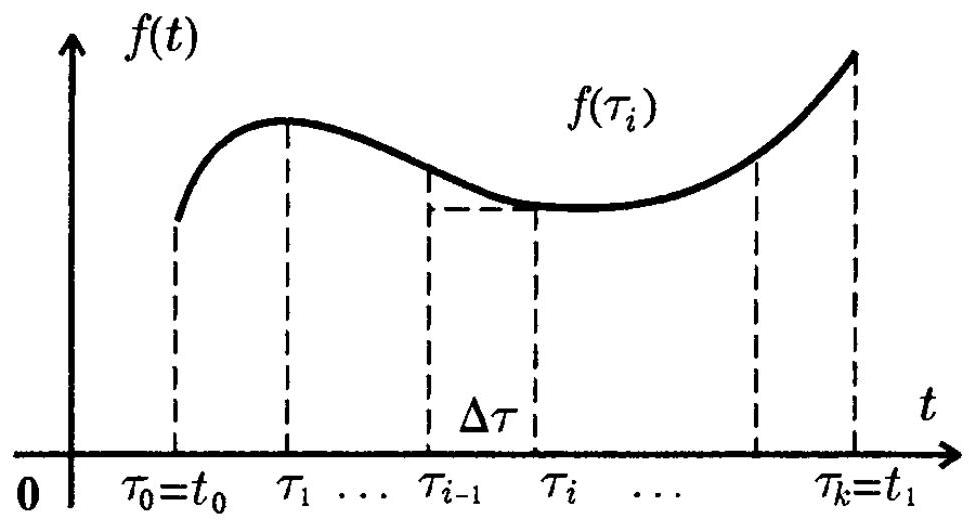
\includegraphics[max width=0.9\textwidth]{images/bo_d547okref24c73bgfch0_53_247_0_969_524_0.jpg}
\end{center}
\hspace*{3em} 

Рис. 12

Для непрерывной или кусочно непрерывной функции f: \({E}^{1} \rightarrow  {E}^{n}\) в математическом анализе хорошо известно понятие интеграла \({\int }_{{t}_{0}}^{{t}_{1}}\mathbf{f}\left( t\right) {dt}\) . Обычно его называют интегралом Римана и определяют соотношением

\[
{\int }_{{t}_{0}}^{{t}_{1}}\mathbf{f}\left( t\right) {dt} = \mathop{\lim }\limits_{{k \rightarrow  \infty }}\mathop{\sum }\limits_{{i = 1}}^{k}\mathbf{f}\left( {\tau }_{i}\right) {\Delta \tau }
\]

где \({\Delta \tau } = \frac{{t}_{1} - {t}_{0}}{k}\) , a точки \({\tau }_{i} = {t}_{0} + {i\Delta \tau },i = 0,1,\ldots ,k\) разбивают отрезок на \(k\) paвных частей (puc. 12).

Для измеримой функции \(\mathbf{f}\left( t\right)\) такой интеграл может не су- ществовать, но понятие интеграла можно распространить и на измеримые функции. Такой интеграл называют интегралом Ле- бега и строят по другой схеме. Соответствующие аккуратные построения приведены в разделе Д16 (см. дополнения).

Оказывается, что если функция \(f\left( t\right)\) кусочно непрерывна, то ее интеграл Лебега совпадает с интегралом Римана. Поэто- му при первом знакомстве с теорией оптимального управления измеримые функции можно представлять себе как кусочно не- прерывные, а интеграл Лебега — интегралом Римана.

\section*{4.2. Многозначные отображения}

Многозначным отображением будем называть произвольную функцию \(F : {E}^{1} \rightarrow \Omega \left( {E}^{n}\right)\), т.е. функцию, аргументом которой является время \(t \in {E}^{1}\), а значениями -- элементы пространства \(\Omega \left( {E}^{n}\right)\), т.е. непустые компактные множества из пространства \(E^{n}\). Таким образом, непустое компактное множество \(F\left( t\right)\) движется со временем \(t\), возможно при этом как-то деформируясь (рис. 13). Так как пространства \(E^{1}\) и \(\Omega \left( {E}^{n}\right)\) метрические (см. лекцию 2), то можно говорить о непрерывности многозначного отображения. Многозначное отображение \(F\left( t\right)\) непрерывно в точке \(t_{0}\), если для любого \(\varepsilon > 0\) существует \(\delta > 0\) такое, что неравенство \(h\left( {F\left( t\right),F\left( {t}_{0}\right)}\right) \leq \varepsilon\) выполняется, как только \(\left| t - {t}_{0}\right| \leq \delta\), т.е.
\[
h\left( {F\left( t\right),F\left( {t}_{0}\right)}\right) \rightarrow 0 \quad \text{при} \quad \left| t - {t}_{0}\right| \rightarrow 0.
\]
По определению хаусдорфова расстояния (см. лекцию 2) это означает, что многозначное отображение \(F\left( t\right)\) непрерывно в точке \({t}_{0}\), если для любого \(\varepsilon > 0\) существует \(\delta > 0\) такое, что при всех \(\left| t - {t}_{0}\right| \leq \delta\) выполняются одновременно следующие два включения:

\[
F\left( t\right)  \subset  F\left( {t}_{0}\right)  + {S}_{\varepsilon }\left( 0\right) ,\;F\left( {t}_{0}\right)  \subset  F\left( t\right)  + {S}_{\varepsilon }\left( 0\right) . \tag{4.2}
\]

\begin{center}
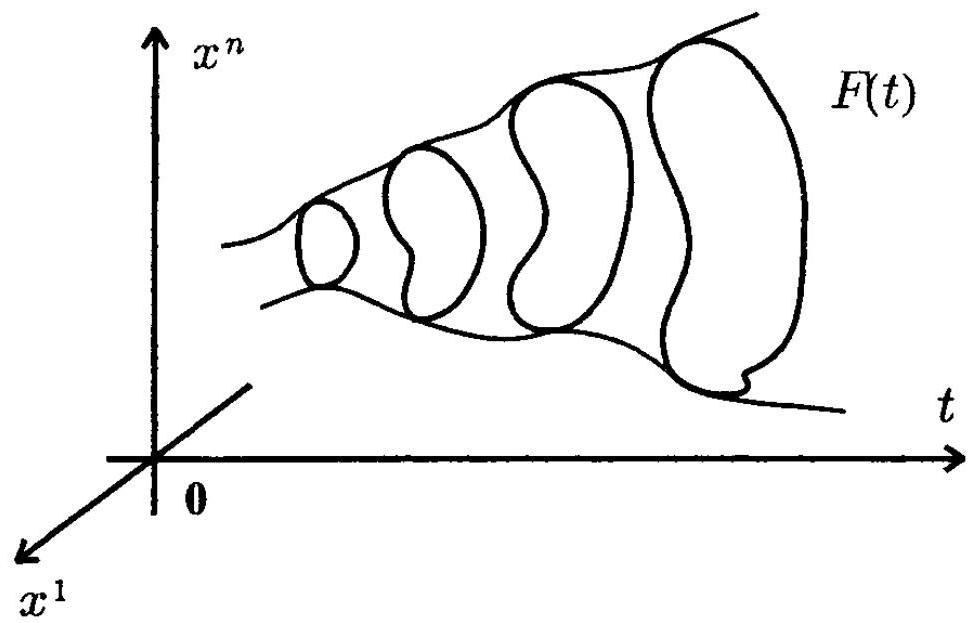
\includegraphics[max width=0.9\textwidth]{images/bo_d547okref24c73bgfch0_54_249_0_976_623_0.jpg}
\end{center}
\hspace*{3em} 

Рис. 13

Многозначное отображение \(F\left( t\right)\) непрерывно, если оно непрерывно в любой точке \({t}_{0} \in {E}^{1}\).

Пример 3. Рассмотрим многозначное отображение \(F : {E}^{1} \rightarrow \Omega \left( {E}^{1}\right)\), определяемое соотношением \(F\left( t\right) = \{ 0\}\) при \(t \leq 0\) и \(F\left( t\right) = t\{ -1,1\}\) при \(t > 0\). Это отображение является однозначным при \(t \leq 0\), и множество \(F\left( t\right)\) при \(t > 0\) состоит из двух точек \(\{ -t,t\}\). График этого отображения показан на рис. 14. Многозначное отображение \(F\left( t\right)\) непрерывно. Действительно, при \(t \leq 0\) непрерывность функции \(F\left( t\right)\) в точке \({t}_{0}\) очевидна. Пусть \(t > 0\). Тогда при достаточно малых значениях \(\left| t - {t}_{0}\right|\) множества \(F\left( {t}_{0}\right)\) и \(F\left( t\right)\) имеют вид \(F\left( {t}_{0}\right) = \left\{ -{t}_{0},{t}_{0}\right\}\), \(F\left( t\right) = \{ -t,t\}\).

Покажем, что алгебра- ическая сумма H(t) = \(= F\left( t\right)  + G\left( t\right)\) двух непре- рывных многозначных ото- бражений \(F\left( t\right)\) и \(G\left( t\right)\) являет- ся отображением непрерыв-

\begin{center}
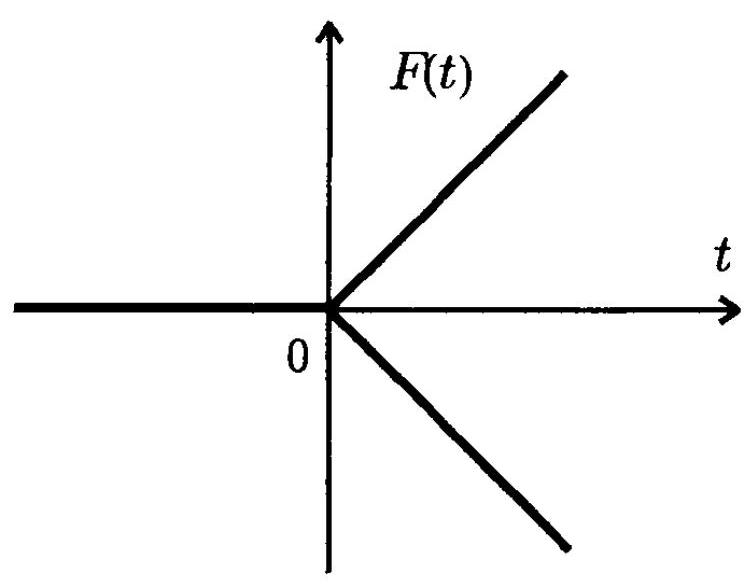
\includegraphics[max width=0.7\textwidth]{images/bo_d547okref24c73bgfch0_55_0_3_749_584_0.jpg}
\end{center}
\hspace*{3em} 

Рис. 14

Хаусдорфовым расстоянием между ними (см. лекцию 2) будет число \(h\left( {F\left( t\right),F\left( {t}_{0}\right)}\right) = \left| t - {t}_{0}\right|\). Следовательно, \(h\left( {F\left( t\right),F\left( {t}_{0}\right)}\right) \rightarrow 0\) при \(\left| t - {t}_{0}\right| \rightarrow 0\), т.е. отображение \(F\left( t\right)\) непрерывно.

\[
F\left( t\right)  \subset  F\left( {t}_{0}\right)  + {S}_{\varepsilon /2}\left( \mathbf{0}\right) ,\;F\left( {t}_{0}\right)  \subset  F\left( t\right)  + {S}_{\varepsilon /2}\left( \mathbf{0}\right) ,
\]

\[
G\left( t\right)  \subset  G\left( {t}_{0}\right)  + {S}_{\varepsilon /2}\left( \mathbf{0}\right) ,\;G\left( {t}_{0}\right)  \subset  G\left( t\right)  + {S}_{\varepsilon /2}\left( \mathbf{0}\right) .
\]

Просуммировав эти множества попарно, получим для отобра- жения \(H\left( t\right)  = F\left( t\right)  + G\left( t\right)\) включения:

\[
H\left( t\right)  \subset  H\left( {t}_{0}\right)  + {S}_{\varepsilon }\left( \mathbf{0}\right) ,\;H\left( {t}_{0}\right)  \subset  H\left( t\right)  + {S}_{\varepsilon }\left( \mathbf{0}\right)
\]

при всех |t-t e) ≤ \(\delta\) ,т.е. отображение \(H\left( t\right)\) непрерывно.

Пусть \(F \in  \Omega \left( {E}^{n}\right)\) , a \(A\left( t\right)  -\) матрица размером \(n \times  n\) , bce элементы которой \({a}_{ij}\left( t\right)\) — непрерывные функции. Покажем, что многозначное отображение \(F\left( t\right)  = A\left( t\right) F\) непрерывно. Для этого зафиксируем число \(\varepsilon  > 0\) и точку \({t}_{0} \in  {E}^{1}\) и покажем,что при малых отклонениях t от t, 0 выполняются включения (4.2).

Напомннм, что нормой матрицы \(A\) называется величина

\[
\parallel A\parallel  = \mathop{\max }\limits_{{x \in  {S}_{1}\left( \mathbf{0}\right) }}\parallel {Ax}\parallel .
\]

Таким образом, всегда справедлива оценка ||A|x|| < ||A||.|x|. Если все элементы матрицы \(A\left( t\right)\) суть непрерывные функции, то и норма матрицы \(A\left( t\right)\)

\[
\parallel A\left( t\right) \parallel  = \mathop{\max }\limits_{{\mathbf{x} \in  {S}_{1}\left( 0\right) }}\parallel A\left( t\right) \mathbf{x}\parallel
\]

— функция непрерывная.

Покажем,что при \(\left| {t - {t}_{0}}\right|  \leq  \delta\) выполняется неравенство

\[
A\left( t\right) F \subset  A\left( {t}_{0}\right) F + {S}_{\varepsilon }\left( \mathbf{0}\right) . \tag{4.3}
\]

Возьмем произвольную точку х ∈ A(t)F. Она имеет представ- ление \(\mathbf{x} = A\left( t\right) \mathbf{f}\) ,где \(\mathbf{f} \in  F\) . To чка х \({\mathbf{x}}_{0} = A\left( {t}_{0}\right) \mathbf{f}\) очевидно принадлежит множеству \(A\left( {t}_{0}\right) F\) . Если мы докажем неравенст- во \(\left\lVert \begin{array}{c} {\mathbf{x} - {\mathbf{x}}_{0}} \end{array} \right\rVert \leq  \varepsilon\) , то включение (4.3) будет выполнено. Имеем соотношение

\[
\left\lVert \begin{array}{c} {\mathbf{x} - {\mathbf{x}}_{0}} \end{array} \right\rVert = \left\lVert \begin{array}{c} {A\left( t\right) \mathbf{f} - A\left( {t}_{0}\right) \mathbf{f}} \end{array} \right\rVert = \left\lVert \begin{array}{c} {\left\lbrack  {A\left( t\right)  - A\left( {t}_{0}\right) }\right\rbrack  \mathbf{f}} \end{array} \right\rVert \leq
\]

\[
\leq  \parallel A\left( t\right)  - A\left( {t}_{0}\right) \parallel  \cdot  \parallel \mathbf{f}\parallel  \leq  \left\lVert \begin{array}{c} {A\left( t\right)  - A\left( {t}_{0}\right) } \end{array} \right\rVert \cdot  \left| F\right| .
\]

В силу непрерывности нормы || \(A\left( t\right)\) || существует δ > 0 такое, что при всех |t- t'0 |< δ выполняется неравенство

\[
\left\lVert \begin{array}{c} {A\left( t\right)  - A\left( {t}_{0}\right) } \end{array} \right\rVert \leq  \frac{\varepsilon }{\left| F\right| }
\]

следовательно, \(\left\lVert \begin{array}{c} {\mathbf{x} - {\mathbf{x}}_{0}} \end{array} \right\rVert \leq  \varepsilon\) и включение (4.3) доказано.

Таким же способом доказывается и включение

\[
A\left( {t}_{0}\right) F \subset  A\left( t\right) F + {S}_{\varepsilon }\left( \mathbf{0}\right) .
\]

Выполнение этих двух включений означает непрерывность ото- бражения \(A\left( t\right) F\) в точке \({t}_{0}\) (см. формулу (4.2)).

Пусть задано многозначное отображение \(F : {E}^{1} \rightarrow  \Omega \left( {E}^{n}\right)\) . Поскольку множество \(F\left( t\right)\) есть непустой компакт, для него можно определить опорную функцию \(c\left( {F\left( t\right) ,\mathbf{\psi }}\right)\) . Если много- значное отображение \(F\left( t\right)\) зафиксировано, то опорная функция \(c\left( {F\left( t\right) ,\psi }\right)\) становится функцией двух аргументов t и ψ, т.е. \(c\left( {F\left( t\right) ,\psi }\right)  : {E}^{1} \times  {E}^{n} \rightarrow  {E}^{1}.\)

Теорема 1. Пусть \(F : {E}^{1} \rightarrow  \Omega \left( {E}^{n}\right)\) есть непрерывное многозначное отображение. Тогда опорная функция \(c\left( {F\left( t\right) ,\psi }\right)\) непрерывна по \(t\) при каждом фиксированном значении \(\psi  \in  {E}^{n}\) . Наоборот, если функция \(c\left( {F\left( t\right) ,\psi }\right)\) непрерывна по \(t\) при каждом фиксированном значении \(\psi  \in  {E}^{n}\) , то многозначное отображение conv \(F\left( t\right)\) непрерывно.

Доказательство. Пусть многозначное отображение F: \({E}^{1} \rightarrow  \Omega \left( {E}^{n}\right)\) непрерывно. Покажем, что опорная функция \(c\left( {F\left( t\right) ,\psi }\right)\) непрерывна по совокупности аргументов t, ф. Дей- ствительно, из свойства 13 опорных функций (см. лекцию 3) следует неравенство

\[
\left| {c\left( {F\left( t\right) ,\psi }\right)  - c\left( {F\left( {t}_{0}\right) ,\psi }\right) }\right|  \leq  \left\lVert \begin{array}{c} {\psi }_{0} \end{array} \right\rVert h\left( {F\left( t\right) ,F\left( {t}_{0}\right) }\right)  +
\]

\[
+ \left\lVert \begin{array}{c} {F\left( {t}_{0}\right) } \end{array} \right\rVert \cdot  \left\lVert \begin{array}{c} {\psi  - {\psi }_{0}} \end{array} \right\rVert + {2h}\left( {F\left( t\right) ,F\left( {t}_{0}\right) }\right) \left\lVert \begin{array}{c} {\psi  - {\psi }_{0}} \end{array} \right\rVert,
\]

правая часть которого стремится к нулю при \(t \rightarrow  {t}_{0},\psi  \rightarrow  {\psi }_{0}\) .

Покажем теперь, что если опорная функция \(c\left( {F\left( t\right) ,\mathbf{\psi }}\right)\) непре- рывна по совокупности аргументов t, ψ, то многозначное ото- бражение conv \(F\left( t\right)\) непрерывно. Согласно свойству 15 опорных функций имеем равенство

\[
h\left( {\operatorname{conv}F\left( t\right) ,\operatorname{conv}F\left( {t}_{0}\right) }\right)  = \mathop{\max }\limits_{{\psi  \in  S}}\left| {c\left( {F\left( t\right) ,\psi }\right)  - c\left( {F\left( {t}_{0}\right) ,\psi }\right) }\right| .
\]

Докажем, что правая часть этого равенства стремится к нулю при \(t \rightarrow  {t}_{0}\) . Допустим противное, т.е. пусть существуют такое число \({\varepsilon }_{0} > 0\) и такая последовательность точек \({t}_{k} \rightarrow  {t}_{0}\) ,что

\[
\mathop{\max }\limits_{{\psi  \in  S}}\left| {c\left( {F\left( t\right) ,\psi }\right)  - c\left( {F\left( {t}_{0}\right) ,\psi }\right) }\right|  \geq  {\varepsilon }_{0}.
\]

Это означает, что существуют точки \({\psi }_{k} \in  S\) такие,что

\[
\left| {c\left( {F\left( {t}_{k}\right) ,{\psi }_{k}}\right)  - c\left( {F\left( {t}_{0}\right) ,{\psi }_{k}}\right) }\right|  \geq  {\varepsilon }_{0}. \tag{4.4}
\]

Выделим из последовательности \{ψ\} подпоследовательность, сходящуюся к точке ф \({\psi }_{0} \in  S\) ,и снова обозначим ее через \{ \({\psi }_{k}\) \}. Применяя свойство 13 опорных функций, получаем неравенство

\[
\left| {c\left( {F\left( {t}_{k}\right) ,{\psi }_{k}}\right)  - c\left( {F\left( {t}_{0}\right) ,{\psi }_{k}}\right) }\right|  \leq
\]

\[
\leq  \left| {c\left( {F\left( {t}_{k}\right) ,{\psi }_{k}}\right)  - c\left( {F\left( {t}_{0}\right) ,{\psi }_{0}}\right) }\right|  + \left| {c\left( {F\left( {t}_{0}\right) ,{\psi }_{0}}\right)  - c\left( {F\left( {t}_{0}\right) ,{\psi }_{k}}\right) }\right|  \leq
\]

\[
\leq  \left| {c\left( {F\left( {t}_{k}\right) ,{\psi }_{k}}\right)  - c\left( {F\left( {t}_{0}\right) ,{\psi }_{0}}\right) }\right|  + \left\lVert \begin{array}{c} {F\left( {t}_{0}\right) } \end{array} \right\rVert \cdot  \left\lVert \begin{array}{c} {{\psi }_{k} - {\psi }_{0}} \end{array} \right\rVert.
\]

В силу непрерывности функции \(c\left( {F\left( t\right) ,\mathbf{\psi }}\right)\) no \(t,\mathbf{\psi }\) правая часть этого неравенства стремится к нулю при \({t}_{k} \rightarrow  {t}_{0},{\mathbf{\psi }}_{k} \rightarrow  {\mathbf{\psi }}_{0}\vdots {\mathcal{T}}_{\mathbf{{TO}}}\) противоречит неравенству (4.4).

Для завершения доказательства теоремы остается только показать, что непрерывность опорной функции \(c\left( {F\left( t\right) ,\psi }\right)\) по со- вокупности аргументов \(\mathbf{t},\mathbf{\psi }\) эквивалентна непрерывности по t для каждого фиксированного вектора ф \(\in  {E}^{n}\) . Для произвольной функции от двух аргументов это, конечно, неверно. Пусть опор- ная функция \(c\left( {F\left( t\right) ,\mathbf{\psi }}\right)\) непрерывна по t. Согласно свойству 13 опорных функций имеем неравенство

\[
\left| {c\left( {F\left( t\right) ,\psi }\right)  - c\left( {F\left( {t}_{0}\right) ,{\psi }_{0}}\right) }\right|  \leq
\]

\[
\leq  \left| {c\left( {F\left( t\right) ,\psi }\right)  - c\left( {F\left( t\right) ,{\psi }_{0}}\right) }\right|  + \left| {c\left( {F\left( t\right) ,{\psi }_{0}}\right)  - c\left( {F\left( {t}_{0}\right) ,{\psi }_{0}}\right) }\right|  \leq
\]

\[
\leq  \left| {F\left( t\right) }\right|  \cdot  \left\lVert \begin{array}{c} {\psi  - {\psi }_{0}} \end{array} \right\rVert + \left| {c\left( {F\left( t\right) ,{\psi }_{0}}\right)  - c\left( {F\left( {t}_{0}\right) ,{\psi }_{0}}\right) }\right| .
\]

Если показать, что величина |F(t)| ограничена при t → t0, то тогда правая часть последнего неравенства стремится к нулю при \(t \rightarrow  {t}_{0},\psi  \rightarrow  {\psi }_{0}\) ,и функция \(c\left( {F\left( t\right) ,\psi }\right)\) непрерывна по сово- купности аргументов \(t,\psi\) .

Предположим противное, т.е. пусть существует такая после- довательность точек \({t}_{k} \rightarrow  {t}_{0}\) ,что \(\left| {{F}_{k}\left( t\right) }\right|  \rightarrow  \infty\) . По определению модуля множества |F| (см. лекцию 2) и следствию из свойства 10 опорных функций справедливы неравенства

\[
\left| F\right|  = \min \left\{  {r : F \subset  {S}_{r}\left( 0\right) }\right\}   =
\]

\[
= \min \{ r : c\left( {F\left( t\right) ,\psi }\right)  \leq  c\left( {{S}_{r}\left( 0\right) ,\psi }\right)  = r,\psi  \in  S\}  =
\]

\[
= \mathop{\max }\limits_{{\psi  \in  S}}c\left( {F\left( t\right) ,\psi }\right) \text{ . } \tag{4.5}
\]

Таким образом, существуют векторы у \({\psi }_{k} \in  S\) такие,что

\[
\left| {F\left( {t}_{k}\right) }\right|  = c\left( {F\left( {t}_{k}\right) ,{\psi }_{k}}\right) . \tag{4.6}
\]

Выделим из последовательности \{ \({\psi }_{k}\) \} подпоследователь- ность, сходящуюся к точке фо с S, и снова обозначим ее через \(\left\{  {\psi }_{k}\right\}\) . Из свойства 13 опорных функций следует неравенство

\[
c\left( {F\left( {t}_{k}\right) ,{\psi }_{k}}\right)  - c\left( {F\left( {t}_{k}\right) ,{\psi }_{0}}\right)  \leq  \left| {F\left( {t}_{k}\right) }\right|  \cdot  \left\lVert \begin{array}{c} {{\psi }_{k} - {\psi }_{0}} \end{array} \right\rVert,
\]

откуда, учитывая равенство (4.6), получаем соотношение

\[
\left| {F\left( {t}_{k}\right) }\right| \left( {1 - \left\lVert \begin{array}{c} {{\psi }_{k} - {\psi }_{0}} \end{array} \right\rVert}\right)  \leq  c\left( {F\left( {t}_{k}\right) ,{\psi }_{0}}\right) .
\]

Поскольку функция \(c\left( {F\left( t\right) ,{\mathbf{\psi }}_{0}}\right)\) непрерывна по \(t\) ,из этого соот- ношения следует ограниченность последовательности |F( \({t}_{k}\) )|, a это противоречит сделанному предположению. Теорема дока- зана.

Следствие. Пусть многозначное отображение \(F : {E}^{1} \rightarrow \; \rightarrow  \Omega \left( {E}^{n}\right)\) max \(o \circ  o\) , что множества F(t) выпуклы при всех \(t \in  {E}^{1}\) . В этом случае многозначное отображение непрерыв- но тогда и только тогда, когда опорная функция с(F(t), ф) непрерывна no t при каждом фиксированном фе S.

Пример 4. Рассмотрим многозначное отображение \(F\) : \(: {E}^{1} \rightarrow  \Omega \left( {E}^{1}\right) ,\) заданное условием \(F\left( t\right)\)  \(=\)  \(\{ 1\}\) при \(t > 0, \; F\left( t\right)  = \{  - 1\}\) nput \(t < 0\) и \(F\left( 0\right)  = \left\lbrack  {-1,1}\right\rbrack\) . График этого ото- бражения показан на рис. 15.

\begin{center}
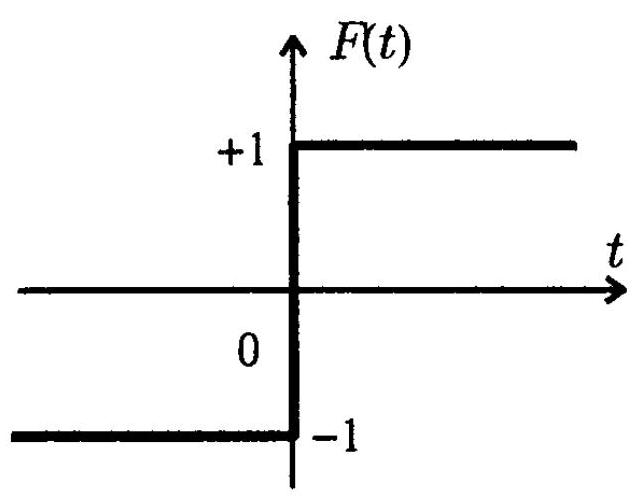
\includegraphics[max width=0.6\textwidth]{images/bo_d547okref24c73bgfch0_59_2_457_642_501_0.jpg}
\end{center}
\hspace*{3em} 

Рис. 15

Очевидно, что во всех точках \(t \neq  0\) это отображение непрерыв- но. Множество \(F\left( t\right)\) выпукло при всех у не го порная функция имеет вид

\[
c\left( {F\left( t\right) ,\psi }\right)  = \begin{cases}  - \psi , & \operatorname{\text{ е }\text{ с }\text{ л }\text{ и }}t < 0, \\  \left| \psi \right| , & \operatorname{\text{ е }\text{ с }\text{ л }\text{ и }}t = 0, \\  \psi , & \operatorname{\text{ е }\text{ с }\text{ л }\text{ и }}t > 0. \end{cases}
\]

Например, при \(\psi  = 1\) эта функ- ция претерпевает разрыв в точ- ке \({\mathbf{t}}_{0} = 0\) . Таким образом, в силу следствия из теоремы 1 многозначное отображение \(F\left( t\right)\) не яв- ляется непрерывным в точке t = 0.

Пример 5. Рассмотрим многозначное отображение F: \({E}^{1} \rightarrow  \Omega \left( {E}^{1}\right)\) ,заданное условием \(F\left( t\right)  = \left\lbrack  {-1,1}\right\rbrack\) при \(t \neq  0\) и \(F\left( 0\right)  = \{ 0\}\) . График этого отображения приведен на рис. 16.

\begin{center}
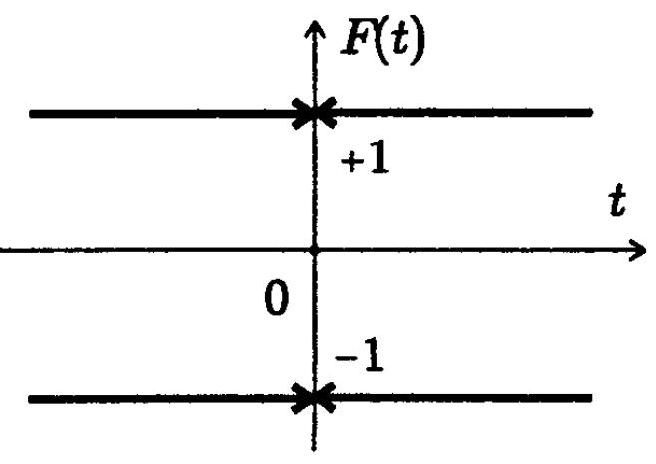
\includegraphics[max width=0.6\textwidth]{images/bo_d547okref24c73bgfch0_59_1_1417_656_464_0.jpg}
\end{center}
\hspace*{3em} 

Рис. 16

Очевидно, что во всех точках \(t \neq  0\) это отображение непрерыв- но. Множество \(F\left( t\right)\) выпукло при всех t ∈ \({E}^{1}\) , и его опорная функция IMMEET BMA

\[
c\left( {F\left( t\right) ,\psi }\right)  = \left\{  \begin{array}{ccc} \left| \psi \right| , & \text{ если } & t \neq  0, \\  0, & \text{ если } & t = 0. \end{array}\right.
\]

Например, для \(\psi  = 1\) эта функ- ция имеет разрыв в точке \({t}_{0} = 0\) . Таким образом, многозначное ото- бражение \(F\left( t\right)\) не является непрерывным в точке \({t}_{0}\) согласно следствию из теоремы 1.

Функция \(f : {E}^{1} \rightarrow  {E}^{n}\) называется однозначной ветвью многозначного отображения \(F : {E}^{1} \rightarrow  \Omega \left( {E}^{n}\right)\) , ecли при всех \(t \in  {E}^{1}\) выполняется включение f(t) ∈ F(t). Ясно, что однознач- ная ветвь \(f\left( t\right)\) всегда существует, поскольку множество F(t) непусто при всех t ∈ \({E}^{n}\) .

Нас будут интересовать такие однозначные ветви f(t), ко- торые можно проинтегрировать на заданном отрезке \(\left\lbrack  {{t}_{0},{t}_{1}}\right\rbrack\) ,т.е. для которых существует интеграл \({\int }_{{t}_{0}}^{{t}_{1}}\mathbf{f}\left( t\right) {dt}\) . Здесь можно было бы ограничиться непрерывными ветвями f(t) и интеграл пони- мать в смысле Римана. Непрерывные однозначные ветви можно выделять для достаточно широкого класса многозначных ото- бражений \(F\left( t\right)\) . Так, в примере 3 существуют две непрерывные однозначные ветви

\[
{f}_{1}\left( t\right)  = \left\{  {\begin{array}{ll} 0, & t \leq  0, \\  t, & t > 0; \end{array}\;{f}_{2}\left( t\right)  = \left\{  \begin{array}{cc} 0, & t \leq  0, \\   - t, & t > 0. \end{array}\right. }\right.
\]

В примере 5 непрерывных ветвей существует много. Например, функции \(f\left( t\right)  \equiv  0,f\left( t\right)  = \sin t\) являются даже гладкими одно- значными ветвями. Однако в примере 4 не существует непре- рывной однозначной ветви f(t) у многозначного отображения \(F\left( t\right)\) . Любая ветвь должна иметь разрыв в точке t = 0 . Но многозначное отображение в примере 4 само не является не- прерывным. Оказывается, что если даже многозначное отобра- жение непрерывно, то у него может не существовать ни одной непрерывной однозначной ветви. Приведем соответствующий пример.

Пример 6. Рассмотрим многозначное отображение F: \(\left\lbrack  {0,1}\right\rbrack   \rightarrow  \Omega \left( {E}^{2}\right)\) ,заданное условием

\[
F\left( t\right)  = \left\{  {\left( \begin{array}{c} \cos \left( {\alpha  + \lg t}\right) \\  \sin \left( {\alpha  + \lg t}\right) \end{array}\right)  : t \leq  \alpha  \leq  {2\pi }}\right\}
\]

при \(0 < t \leq  1\) и \(F\left( 0\right)  = S\) . При \(t \neq  0\) множество \(F\left( t\right)\) представля- ет собой часть дуги на единичной окружности в плоскости \({E}^{2}\) (рис. 17). При этом множеству \(F\left( t\right)\) не хватает до всей окруж- ности \(S\) дуги с центральным углом в t радиан и начало этой вы- брошенной части дуги имеет угол, равный \(\lg t\) . Таким образом, при \(t \rightarrow  0\) длина выброшенной части дуги стремится к нулю, но ее начало стремится к —о. Отображение \(F\left( t\right)\) непрерывно на отрезке [0,1]. Любая однозначная ветвь \(f\left( t\right)  \in  F\left( t\right)\) должна при \(t \rightarrow  0\) cosepшать бесконечное число оборотов по окружности S, иначе она пересечет выброшенную часть дуги и уже не будет

Oтсутствие непрерыв- ной ветви у отображения \(F\left( t\right)\) в этом примере объ- ясняется тем, что множес- тво F(t) было невыпукло при \(t > 0\) . Но именно такая ситуация часто встречает- ся в задачах оптимального управления. ветвью. Но такая функция \(f\left( t\right)\) не имеет предела при \(t \rightarrow  0\) . Cлeдовательно, у отображения \(F\left( t\right)\) нет ни од- ной непрерывной однознач- ной ветви.

\begin{center}
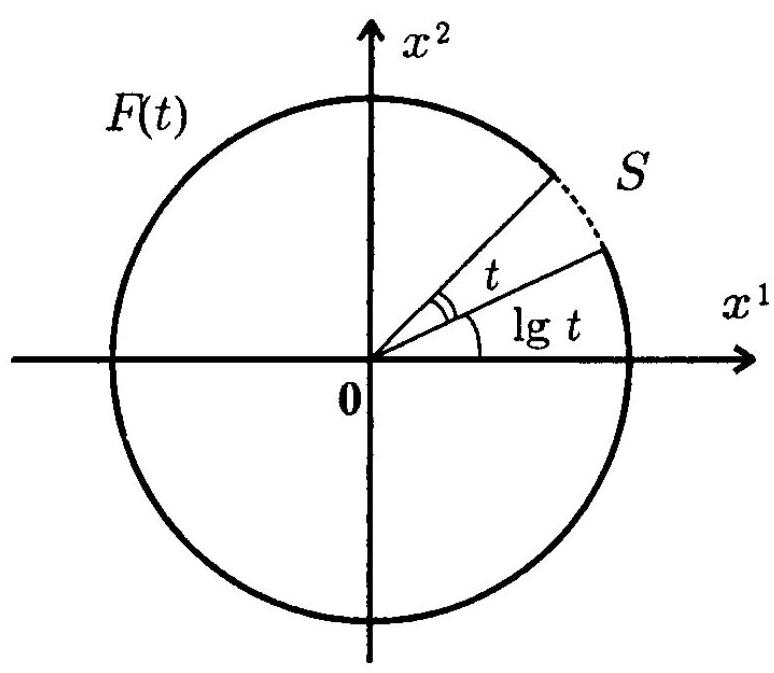
\includegraphics[max width=0.7\textwidth]{images/bo_d547okref24c73bgfch0_61_3_12_774_673_0.jpg}
\end{center}
\hspace*{3em} 

Рис. 17

Приведенные соображения наводят на мысль рассматривать измеримые однозначные ветви и интегрировать их в смысле Ле- бега. Оказывается, что у непрерывного многозначного отобра- жения уже всегда существует измеримая ветвь. Сформулируем это в виде теоремы.

Теорема 2. Пусть многозначное отображение \(F : I \rightarrow  \Omega \left( {E}^{n}\right)\) непрерывно на отрезке \(I = \left\lbrack  {{t}_{0},{t}_{1}}\right\rbrack\). Тогда у него существует измеримая на этом отрезке \(I\) однозначная ветвь \(f\left( t\right)  \in  F\left( t\right)\). Более того, если \(\psi \in S\) -- произвольный фиксированный вектор, то существует измеримая ветвь \(f\left( t\right)\) такая, что при всех \(t \in I\) выполняется включение

\[
f\left( t\right)  \in  \mathcal{U}\left( {F\left( t\right) ,\psi }\right) ,
\]

т.е. измеримая ветвь f(t) при всех t ∈ I принадлежит опор- ному множеству \(\mathcal{U}\left( {F\left( t\right) ,\mathbf{\psi }}\right)\) в направлении \(\mathbf{\psi } \in  S\) .

Доказательство теоремы 2 приводится в разделе Д7 (см. до- полнения, следствие 2 к теореме 1)

\section*{4.3. Задачи}

1. Докажите, что многозначное отображение \(F : {E}^{1} \rightarrow \; \rightarrow  \Omega \left( {E}^{n}\right)\) , onределяемое условием

\[
F\left( t\right)  = \left\{  \begin{array}{lll} {S}_{r\left( t\right) }\left( {a\left( t\right) }\right) , & \mathrm{{\text{ е }\text{ с }\text{ л }\text{ и }}} & t \neq  0, \\  0, & \mathrm{{\text{ е }\text{ с }\text{ л }\text{ и }}} & t = 0, \end{array}\right.
\]

непрерывно тогда и только тогда, когда функции \(r : {E}^{1} \rightarrow  {E}^{1}\) и \(a : {E}^{1} \rightarrow  {E}^{n}\) непрерывны.

2. Будет ли многозначное отображение \(F = t \cdot  {S}_{\sin \frac{1}{t}}\left( 0\right)\) не- прерывным?

3. Докажите, что образ любого компактного множества \(K \subset  {E}^{1}\) при непрерывном многозначном отображении \(F : {E}^{1} \rightarrow \; \rightarrow  \Omega \left( {E}^{n}\right)\) , т.е. множество

\[
F\left( K\right)  = \mathop{\bigcup }\limits_{{t \in  K}}F\left( t\right)
\]

является компактом в пространстве E".

4. Докажите, что прообраз любого открытого множества \(P \subset  {E}^{n}\) при непрерывном многозначном отображении \(F : {E}^{1} \rightarrow \; \rightarrow  \Omega \left( {E}^{n}\right)\) , т.е. множество

\[
\{ t \in  {E}^{1} : F\left( t\right)  \subset  P\}
\]

является открытым в пространстве E1.

\({5}^{ * }\) . Многозначное отображение \(F : {E}^{1} \rightarrow  \Omega \left( {E}^{n}\right)\) называется полунепрерывным сверху в точке и, если для любого числа \(\varepsilon  > 0\) cyществует число \(\delta  > 0\) такое,что при всех |t-to|≤ \(\delta\) справедливо включение

\[
F\left( t\right)  \subset  F\left( {t}_{0}\right)  + {S}_{\varepsilon }\left( \mathbf{0}\right) .
\]

Докажите, что образ F(K) любого компактного множества \(K \subset  {E}^{1}\) при полунепрерывном сверху отображении является компактом в \({E}^{n}\) .

6*. Докажите, что график полунепрерывного сверху много- значного отображения \(F : {E}^{1} \rightarrow  \Omega \left( {E}^{n}\right)\) , т.е. множество

\[
\left\{  {\left( {t,\mathbf{x}}\right)  \in  {E}^{1} \times  {E}^{n} : t \in  {E}^{1},\mathbf{x} \in  F\left( t\right) }\right\}
\]

является замкнутым в пространстве \({E}^{1} \times  {E}^{n}\) .

\({7}^{ * }\) . Пусть многозначное отображение \(F : {E}^{1} \rightarrow  \Omega \left( {E}^{n}\right)\) непре- рывно и множество \(F\left( t\right)\) выпукло при всех t ∈ \({E}^{1}\) . Докажите, что существует непрерывная однозначная ветвь \(f\left( t\right)\) отображе- ния \(F\left( t\right)\) .

\({8}^{ * }\) . Пусть многозначное отображение \(F : {E}^{1} \rightarrow  \Omega \left( {E}^{n}\right)\) непре- рывно и множество \(F\left( t\right)\) выпукло при всех t ∈ \({E}^{1}\) . Далее, пусть заданы точки \({t}_{0} \in  {E}^{1},{\mathbf{x}}_{0} \in  F\left( {t}_{0}\right)\) . Докажите, что существует непрерывная однозначная ветвь f(t) отображения \(F\left( t\right)\) , yдовле- творяющая условию \(f\left( {t}_{0}\right)  = {x}_{0}\) .

\({9}^{ * }\) . Многозначное отображение \(F : {E}^{1} \rightarrow  \Omega \left( {E}^{n}\right)\) называет- ся полунепрерывным снизу в точке б, если для любого числа \(\varepsilon  > 0\) cymecтвует число \(\delta  > 0\) raкое,что при всех |t-to| ≤ \(\delta\) справедливо включение

\[
F\left( {t}_{0}\right)  \subset  F\left( t\right)  + {S}_{\varepsilon }\left( \mathbf{0}\right) .
\]

Докажите, что если многозначное отображение \(F : {E}^{1} \rightarrow  \Omega \left( {E}^{n}\right)\) полунепрерывно снизу и множество F(t) выпукло при всех \(t \in  {E}^{1}\) , то существует непрерывная однозначная ветвь f(t) отображения \(F\left( t\right)\) .

\section*{ЛЕКЦИЯ 5}

\begin{itemize}\relax
\item\relax Интеграл от многозначного отображения, его ос- новные свойства.
\end{itemize}

\begin{itemize}\relax
\item\relax Теорема Ляпунова.
\end{itemize}

\section*{5.1. Интегрирование многозначных отображений}

Пусть заданы отрезок времени \(I = \left\lbrack  {{t}_{0},{t}_{1}}\right\rbrack\) и некоторое ото- бражение \(F : I \rightarrow  \Omega \left( {E}^{n}\right)\) . Интегралом от многозначного ото- бражения \(F\left( t\right)\) на отрезке \(I\) называется множество

\[
G = {\int }_{{t}_{0}}^{{t}_{1}}F\left( t\right) {dt} = \left\{  {{\int }_{{t}_{0}}^{{t}_{1}}\mathbf{f}\left( t\right) {dt} : \mathbf{f}\left( t\right)  \in  F\left( t\right) }\right\}  .
\]

Здесь в правой части интеграл Лебега берется по всем одно- значным ветвям отображения \(F\left( t\right)\) ,для которых он существует. Ясно, что \(G\) является подмножеством пространства E".

Теорема 1. Пусть многозначное отображение \(F\left( t\right)\) непре- рывно на отрезке I = [t, t, ]. Тогда интеграл от этого много- значного отображения является непустым компактным мно- HEECMEOM B NPOCMPAHCMEE \({E}^{n}\) , т.е.

\[
G = {\int }_{{t}_{0}}^{{t}_{1}}F\left( t\right) {dt} \in  \Omega \left( {E}^{n}\right) .
\]

Более того, множество G выпукло.

Доказательство. Покажем, что в предположениях тео- ремы множество G непусто. Действительно, по теореме 2 (см. лекцию 4) существует хотя бы одна измеримая ветвь f(t) много- значного отображения \(F\left( t\right)\) . Для модуля множества |F(t)| спра- ведливо равенство (см. формулу (4.5))

\[
\left| {F\left( t\right) }\right|  = \mathop{\max }\limits_{{\psi  \in  S}}c\left( {F\left( t\right) ,\psi }\right)
\]

Поскольку отображение \(F\left( t\right)\) непрерывно, его опорная функция \(c\left( {F\left( t\right) ,\psi }\right)\) непрерывна по \(t\) (теорема 1, лекция 4), а следова- тельно, непрерывна и функция \(\left| {F\left( t\right) }\right|\) . Тогда она ограничена на отрезке времени \(I = \left\lbrack  {{t}_{0},{t}_{1}}\right\rbrack\) , т.е. \(\left| {F\left( t\right) }\right|  \leq  k\) при всех \(t \in  I\) . Таким образом, для измеримой ветви \(f\left( t\right)\) справедливо неравенство

\[
\parallel f\left( t\right) \parallel  \leq  \left| {F\left( t\right) }\right|  \leq  k. \tag{5.1}
\]

Согласно свойству 8 интеграла Лебега (см. раздел Д6 до- полнений) эта ветвь \(f\left( t\right)\) интегрируема и \({\int }_{{t}_{0}}^{{t}_{1}}f\left( t\right) {dt} \in  G\) , т.е. множество \(G\) непусто.

Покажем теперь, что множество G ограничено. Действи- тельно, пусть \(g \in  G\) . Тогда \(g = {\int }_{{t}_{0}}^{{t}_{1}}f\left( t\right) {dt}\) , где \(f\left( t\right)\) — некоторая ветвь многозначного отображения \(F\left( t\right)\) . Согласно свойству 3 интеграла Лебега (см. раздел Д6 дополнений) и соотношению (5.1) имеем

\[
\parallel \mathbf{g}\parallel  = \left\lVert \begin{array}{c} {{\int }_{{t}_{0}}^{{t}_{1}}\mathbf{f}\left( t\right) {dt}} \end{array} \right\rVert \leq  {\int }_{{t}_{0}}^{{t}_{1}}\parallel \mathbf{f}\left( t\right) \parallel {dt} \leq  {\int }_{{t}_{0}}^{{t}_{1}}\mathbf{k}{dt} = \mathbf{k}\left( {{t}_{1} - {t}_{0}}\right)  = l.
\]

Таким образом, \(G \subset  {S}_{l}\left( 0\right)\) , т.е. множество \(G\) ограничено.

Для завершения доказательства теоремы остается доказать замкнутость и выпуклость множества G. Доказательство этих фактов приведено в разделе Д7 дополнений. Докажем только выпуклость \(G\) в частном случае, когда множество \(F\left( t\right)\) выпукло при всех t ∈ I.

Пусть заданы точки \({\mathbf{g}}_{1},{\mathbf{g}}_{2} \in  G\) и число 0 ≤ \(\lambda  \leq  1\) . По определению интеграла, существуют интегрируемые функции \({f}_{1}\left( t\right)\) и \({f}_{2}\left( t\right)\) rakue,что

\[
{\mathbf{g}}_{1} = {\int }_{{t}_{0}}^{{t}_{1}}{\mathbf{f}}_{1}\left( t\right) {dt},\;{\mathbf{g}}_{2} = {\int }_{{t}_{0}}^{{t}_{1}}{\mathbf{f}}_{2}\left( t\right) {dt}
\]

и \({\mathbf{f}}_{1}\left( t\right)  \in  F\left( t\right) ,{\mathbf{f}}_{2}\left( t\right)  \in  F\left( t\right)\) . Согласно свойству 3 (см. раздел Д6 дополнений) интеграла Лебега имеем

\[
\lambda {g}_{1} + \left( {1 - \lambda }\right) {g}_{2} = \lambda {\int }_{{t}_{0}}^{{t}_{1}}{f}_{1}\left( t\right) {dt} + \left( {1 - \lambda }\right) {\int }_{{t}_{0}}^{{t}_{1}}{f}_{2}\left( t\right) {dt} =
\]

\[
= {\int }_{{t}_{0}}^{{t}_{1}}\left\lbrack  {\lambda {f}_{1}\left( t\right)  + \left( {1 - \lambda }\right) {f}_{2}\left( t\right) }\right\rbrack  {dt}.
\]

Поскольку множество \(F\left( t\right)\) выпукло при всех t ∈ \(I\) , то \(\lambda {\mathbf{f}}_{1}\left( t\right)  + \; + \left( {1 - \lambda }\right) {\mathbf{f}}_{2}\left( t\right)  \in  F\left( t\right)\) и,следовательно, \(\lambda {\mathbf{g}}_{1} + \left( {1 - \lambda }\right) {\mathbf{g}}_{2} \in  G\) ,т.е. множество \(G\) выпукло. Теорема доказана.

Если даже ограничиться только непрерывными многознач- ными отображениями \(F\left( t\right)\) , \(\mathrm{y}\) которых множества \(F\left( t\right)\) выпук- лы, то замкнутости интеграла может не быть, если этот ин- теграл брать в смысле Римана по всем кусочно непрерывным ветвям \(f\left( t\right)\) отображения \(F\left( t\right)\) . Замыкание получится, если доба- вить интегралы (теперь по Лебегу) по всем измеримым ветвям \(f\left( t\right)  \in  F\left( t\right)\) .

Теорема 1 представляет собой частный случай известной теоремы Ляпунова. Это очень глубокий математический ре- зультат, который широко применяют в современной матема- тике. Мы тоже будем использовать его в теории оптимального управления. Полное доказательство теоремы Ляпунова опирает- ся на большое количество вспомогательных фактов (см. разде- лы Д4 — Д6 дополнений) и приведено в разделе Д7 дополнений.

Пример 1. Рассмотрим многозначное отображение \(F\) : \(\left\lbrack  {0,1}\right\rbrack   \rightarrow  \Omega \left( {E}^{1}\right)\) , ompeделенное соотношением \(F\left( t\right)  = t\{  - 1,1\}\) (puc. 18). Найдем интеграл \(G = {\int }_{0}^{1}F\left( t\right) {dt}\) . Oчевидно,что макси- мальное значение \(g \in  G\) paвно \(\frac{1}{2}\) и достигается на непрерывной однозначной ветви \(f\left( t\right)  = t\) ,так как \({\int }_{0}^{1}{tdt} = \frac{1}{2}\) . Toчно так же минимальное значение \(g \in  G\) равно \(- \frac{1}{2}\) и достигается на непре- рывной однозначной ветви f(t) = -t, так как \({\int }_{0}^{1}\left( {-t}\right) {dt} =  - \frac{1}{2}\) . Больше непрерывных ветвей y отображения \(F\left( t\right)\) нет. Таким об- pa30м, \(u\) меем \(G \subset  \left\lbrack  {-\frac{1}{2},\frac{1}{2}}\right\rbrack\) . Te- перь можно воспользоваться тео- ремой 1, из которой следует, что множество \(G\) выпукло. Cледова- тельно, \(G = \left\lbrack  {-\frac{1}{2},\frac{1}{2}}\right\rbrack\) . Ho чтобы вы- яснить, почему интеграл от мно- гозначного отображения является множеством выпуклым независимо от того, являются ли множества \(F\left( t\right)\) выпуклыми при \(t \in  I\) или нет, докажем,что \(G = \left\lbrack  {-\frac{1}{2},\frac{1}{2}}\right\rbrack\) без помо- щи теоремы 1.

\begin{center}
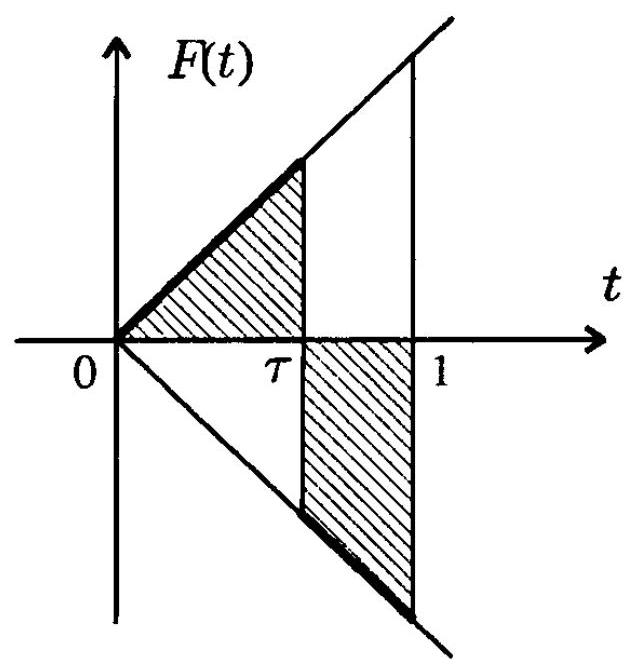
\includegraphics[max width=0.6\textwidth]{images/bo_d547okref24c73bgfch0_66_840_1429_631_672_0.jpg}
\end{center}
\hspace*{3em} 

Рис. 18

Мы уже доказали, что \(G \subset  \left\lbrack  {-\frac{1}{2},\frac{1}{2}}\right\rbrack\) . Пусть теперь g — про- извольная точка отрезка [—2, 1]. Для того чтобы доказать, что \(g \in  G\) , нужно показать существование такой однозначной ветви \(f\left( t\right)\) из многозначного отображения \(F\left( t\right)\) ,что ее интеграл Лебега равен \(g\) . Такая ветвь будет уже разрывной и задается условием

\[
f\left( t\right)  = \left\{  \begin{array}{ccc} t, & \operatorname{ec\text{ л }\text{ и }} & 0 \leq  t \leq  \tau \\   - t, & \operatorname{ec\text{ л }\text{ и }} & \tau  < t \leq  1 \end{array}\right.
\]

где \(\tau  = \sqrt{g + \frac{1}{2}}\) (см. рис. 18). Очевидно, функция \(f\left( t\right)\) интегри- руема по Лебегу и \({\int }_{0}^{1}f\left( t\right) {dt} = g\) . Это означает,что [- \(\frac{1}{2},\frac{1}{2}\rbrack  \subset  G \; u,\) таким образом, \(G = \left\lbrack  {-\frac{1}{2},\frac{1}{2}}\right\rbrack\) .

Для интеграла от многозначного отображения можно опре- делить опорную функцию

\[
c\left( {G,\psi }\right)  = \mathop{\max }\limits_{{g \in  G}}\langle g,\psi \rangle .
\]

Теорема 2. Пусть многозначное отображение \(F\left( t\right)\) непре- рывно на отрезке \(I = \left\lbrack  {{t}_{0},{t}_{1}}\right\rbrack\) . Тогда имеет место равенство

\[
c\left( {{\int }_{{t}_{0}}^{{t}_{1}}F\left( t\right) {dt},\psi }\right)  = {\int }_{{t}_{0}}^{{t}_{1}}c\left( {F\left( t\right) ,\psi }\right) {dt}. \tag{5.2}
\]

Показательство. Интеграл в правой части равенства (5.2) существует, так как опорная функция \(c\left( {F\left( t\right) ,\psi }\right)\) непрерыв- на по t.

Зафиксируем произвольный вектор \(\psi  \in  S\) . Пусть \(G = \; = {\int }_{{t}_{0}}^{{t}_{1}}F\left( t\right) {dt}\) и максимум опорной функции \(c\left( {G,\psi }\right)\) достигается на векторе g* ∈ \(G\) , т.е. \(c\left( {G,\mathbf{\psi }}\right)  = \left\langle  {{\mathbf{g}}^{ * },\mathbf{\psi }}\right\rangle\) . По определению интег- рала существует интегрируемая однозначная ветвь \(f\left( t\right)  \in  F\left( t\right)\) такая, что \({\mathbf{g}}^{ * } = {\int }_{{t}_{0}}^{{t}_{1}}\mathbf{f}\left( t\right) {dt}\) . Согласно следствию из свойства 6 опорных функций (см. лекцию 3) имеем \(\langle \mathbf{f}\left( t\right) ,\mathbf{\psi }\rangle  \leq  c\left( {F\left( t\right) ,\mathbf{\psi }}\right)\) . Следовательно, в силу свойства 5 интеграла Лебега (см. раз- дел Д6 дополнений), получаем неравенство

\[
{\int }_{{t}_{0}}^{{t}_{1}}\langle \mathbf{f}\left( t\right) ,\psi \rangle {dt} \leq  {\int }_{{t}_{0}}^{{t}_{1}}c\left( {F\left( t\right) ,\psi }\right) {dt}.
\]

Таким образом,имеем неравенство

\[
c\left( {G,\psi }\right)  = \left\langle  {{\mathbf{g}}^{ * },\psi }\right\rangle   = {\int }_{{t}_{0}}^{{t}_{1}}\langle \mathbf{f}\left( t\right) ,\psi \rangle {dt} \leq  {\int }_{{t}_{0}}^{{t}_{1}}c\left( {F\left( t\right) ,\psi }\right) {dt}. \tag{5.3}
\]

Согласно теореме 2 (см. лекцию 4) у отображения \(\mathcal{U}\left( {F\left( t\right) ,\psi }\right)\) существует измеримая однозначная ветвь \({\mathbf{f}}^{ * }\left( t\right)\) . В силу оценки \(\left| {\mathcal{U}\left( {F\left( t\right) ,\psi }\right) }\right|  \leq  \left| {F\left( t\right) }\right|  \leq  k\) эта ветвь f*(t) интегрируема на отрез- ке \(I\) , \(c\) ледовательно, \(\mathbf{g} = {\int }_{{t}_{0}}^{{t}_{1}}{\mathbf{f}}^{ * }\left( t\right) {dt} \in  G\) и \(\langle \mathbf{g},\mathbf{\psi }\rangle  \leq  c\left( {G,\mathbf{\psi }}\right)\) . По определению опорного множества имеем равенство \(c\left( {F\left( t\right) ,\mathbf{\psi }}\right)  = \; = \langle {\mathbf{f}}^{ * }\left( t\right) ,\mathbf{\psi }\rangle\) . Таким образом,справедливо неравенство

\[
{\int }_{{t}_{0}}^{{t}_{1}}c\left( {F\left( t\right) ,\psi }\right) {dt} = {\int }_{{t}_{0}}^{{t}_{1}}\left\langle  {{\mathbf{f}}^{ * }\left( t\right) ,\psi }\right\rangle  {dt} = \langle \mathbf{g},\mathbf{\psi }\rangle  \leq  c\left( {G,\mathbf{\psi }}\right) . \tag{5.4}
\]

Из неравенств (5.3) и (5.4) теперь следует равенство (5.2). Teo- рема доказана.

С помощью теремы 2 можно довольно просто находить ин- тегралы от многозначных отображений \(F\left( t\right)\) . Действительно, для этого достаточно в соответствии с формулой (5.2) постро- ить опорную функцию \(c\left( {F\left( t\right) ,\mathbf{\psi }}\right)\) ,проинтегрировать уже одно- значную функцию \(c\left( {F\left( t\right) ,\mathbf{\psi }}\right)\) no \(t\) при каждом значении \(\mathbf{\psi } \in  {E}^{n}\) , а затем восстановить по полученной опорной функции \(c\left( {G,\mathbf{\psi }}\right)\) непустое выпуклое компактное множество G. Заметим, что для восстановления выпуклого множества G по его опорной функции \(c\left( {G,\mathbf{\psi }}\right)\) достаточно подобрать такое множество \(F\) ,чтобы его опорная функция \(c\left( {F,\mathbf{\psi }}\right)\) совпадала с \(c\left( {G,\mathbf{\psi }}\right)\) . Тогда согласно следствию из свойства 2 опорных функций (см. лекцию 3) будем иметь \(G = F\) . Проиллюстрируем это на примере.

Пример 2. Найдем интеграл \(G = {\int }_{-\pi }^{\pi }F\left( t\right) {dt}\) or многознач- ного отображения \(F : \left\lbrack  {-\pi ,\pi }\right\rbrack   \rightarrow  \Omega \left( {E}^{2}\right)\) ,которое имеет вид

\[
F\left( t\right)  = A\left( t\right) \{  - v,v\} , \tag{5.5}
\]

где A — матрица размером 2 × 2, а v — вектор на плоскости \({E}^{2}\) . Таким образом, множество F(t) является образом постоян- ного множества \{−•v, v\}, состоящего из двух точек - v и v, при отображении \(A\left( t\right)\) . Пусть, далее,

\[
A\left( t\right)  = \left( \begin{array}{cc} \sin t & \operatorname{tg}t \\  \cos t & \operatorname{ctg}t \end{array}\right) ,\;v = \left( {1,0}\right) .
\]

Для построения интеграла \(G\) найдем сначала его опорную функ- цию \(c\left( {G,\mathbf{\psi }}\right)\) . Из теоремы 2, формулы (5.5) и свойства 4 опорных функций (см. лекцию 3) следует

\[
c\left( {G,\psi }\right)  = c\left( {{\int }_{-\pi }^{\pi }F\left( t\right) {dt},\psi }\right)  = {\int }_{-\pi }^{\pi }c\left( {F\left( t\right) ,\psi }\right) {dt} =
\]

\[
= {\int }_{-\pi }^{\pi }c\left( {A\left( t\right) \{  - \mathbf{v},\mathbf{v}\} ,\mathbf{\psi }}\right) {dt} = {\int }_{-\pi }^{\pi }c\left( {\{  - \mathbf{v},\mathbf{v}\} ,{A}^{ * }\left( t\right) \mathbf{\psi }}\right) {dt}.
\]

Очевидно,что опорная функция множества \(\{  - v,v\}\) имеет вид

\[
c\left( {\{  - \mathbf{v},\mathbf{v}\} ,\mathbf{\psi }}\right)  = \left| {\langle \mathbf{v},\mathbf{\psi }\rangle }\right| .
\]

Таким образом, выполняется равенство

\[
c\left( {G,\psi }\right)  = {\int }_{-\pi }^{\pi }\left| \left\langle  {v,{A}^{ * }\left( t\right) \psi }\right\rangle  \right| {dt} = {\int }_{-\pi }^{\pi }\left| {\langle A\left( t\right) v,\psi \rangle }\right| {dt}.
\]

Подставив в это выражение конкретные значения матрицы \(A\left( t\right)\) и вектора v, получим

\[
c\left( {G,\psi }\right)  = {\int }_{-\pi }^{\pi }\left| {{\psi }^{1}\sin t + {\psi }^{2}\cos t}\right| {dt}.
\]

3апишем координаты вектора \(\psi  \in  {E}^{2}\) ввиде

\[
{\psi }^{1} = \parallel \psi \parallel \cos \alpha ,\;{\psi }^{2} = \parallel \psi \parallel \sin \alpha .
\]

Тогда имеем

\[
c\left( {G,\psi }\right)  = {\int }_{-\pi }^{\pi }\parallel \psi \parallel  \cdot  \left| {\sin \left( {t + \alpha }\right) }\right| {dt} = 4\parallel \psi \parallel .
\]

Итак, найдена опорная функция интеграла G, а именно, \(c\left( {G,\mathbf{\psi }}\right)  = 4\parallel \mathbf{\psi }\parallel\) . Ho опорная функция шара \({S}_{4}\left( \mathbf{0}\right)\) также име- ет вид \(c\left( {{S}_{4}\left( \mathbf{0}\right) ,\mathbf{\psi }}\right)  = 4\parallel \mathbf{\psi }\parallel\) . Таким образом, опорные функции двух множеств G и 8,4(0) совпадают. А так как эти множества выпуклые, то в силу следствия из свойства 11 опорных функций (см. лекцию 3) они совпадают. Следовательно, \(G = {S}_{4}\left( \mathbf{0}\right)\) .

Заметим, что в примере 2 невозможно построить интеграл \(G\) ,используя непосредственно определение интеграла, как это было сделано в примере 1. Для этого потребовалось бы интегри- ровать бесконечное число однозначных ветвей f(t) многознач- ного отображения \(F\left( t\right)\) . В то же время с помощью теоремы 2 мы сделали это без особого труда.

Пример 3. Найдем интеграл от многозначного отображения \(F\left( t\right)\) ,принимающего постоянное значение \(F\left( t\right)  \equiv  F,F \in  \Omega \left( {E}^{n}\right)\) . Воспользовавшись формулой (5.2), получим выражение

\[
c\left( {{\int }_{{t}_{0}}^{{t}_{1}}{Fdt},\psi }\right)  = {\int }_{{t}_{0}}^{{t}_{1}}c\left( {F,\psi }\right) {dt} = \left( {{t}_{1} - {t}_{0}}\right) c\left( {F,\psi }\right) .
\]

Но такую же опорную функцию имеет выпуклое компактное множество ( \({t}_{1} - {t}_{0}\) ) conv \(F\) , rax как согласно свойствам опорных функций справедливы равенства

\[
c\left( {\left( {{t}_{1} - {t}_{0}}\right) \operatorname{conv}F,\psi }\right)  = \left( {{t}_{1} - {t}_{0}}\right) c\left( {\operatorname{conv}F,\psi }\right)  = \left( {{t}_{1} - {t}_{0}}\right) c\left( {F,\psi }\right) .
\]

Таким образом, эти выпуклые компактные множества совпада- ют, т.е.

\[
{\int }_{{t}_{0}}^{{t}_{1}}{Fdt} = \left( {{t}_{1} - {t}_{0}}\right) \operatorname{conv}F
\]

Рассмотрим теперь интеграл от многозначной функции с переменным верхним пределом, т.е. функцию

\[
G\left( \tau \right)  = {\int }_{{t}_{0}}^{\tau }F\left( t\right) {dt}
\]

где \(\tau \in \left[ t_{0},t_{1}\right]\). В силу теоремы 1 эта функция отображает отрезок \(I = \left[ t_{0},t_{1}\right]\) в метрическое пространство \(\Omega \left( E^{n}\right)\).

Теорема 3. Пусть многозначное отображение \(F : I \rightarrow \Omega \left( E^{n}\right)\) непрерывно на отрезке \(I\). Тогда многозначное отображение
\[
G\left( \tau \right) = \int_{t_{0}}^{\tau} F\left( t\right)\,dt
\]
также непрерывно на отрезке \(I\).

Доказательство. Согласно теореме 2 имеем

\[
c\left( {G\left( \tau \right) ,\psi }\right)  = {\int }_{{t}_{0}}^{\tau }c\left( {F\left( t\right) ,\psi }\right) {dt}.
\]

Таким образом, функция \(c\left( G\left( \tau \right),\psi \right)\) непрерывна по \(\tau\) при каждом фиксированном значении \(\psi \in E^{n}\). Множество \(G\left( \tau \right)\) выпукло согласно теореме 1. Следовательно, в силу теоремы 1 (см. лекцию 4) многозначное отображение \(G\left( \tau \right)\) непрерывно. Теорема доказана.

\section*{5.2. Задачи}

1. Найдите интеграл \(G = {\int }_{-{2\pi }}^{2\pi }F\left( t\right) {dt}\) от многозначного ото- бражения \(F : \left\lbrack  {-{2\pi },{2\pi }}\right\rbrack   \rightarrow  \Omega \left( {E}^{2}\right)\) , которое имеет вид \(F\left( t\right)  = \; = A\left( t\right) \{  - v,v\}\) ,где

\[
A\left( t\right)  = \left( \begin{array}{cc} 3\sin t &  - \cos {3t} \\  7\cos {3t} & \sin {3t} \end{array}\right) ,\;v = \left( {0,2}\right) .
\]

2. Найдите интеграл \({\int }_{{t}_{0}}^{{t}_{1}}F\left( t\right) {dt}\) ,где \(F\left( t\right)\) — map в про- странстве \({E}^{n}\) paдиуса \(r\left( t\right)\) c центром в точке a(t), т.е. \(F\left( t\right)  = \; = {S}_{r\left( t\right) }\left( {a\left( t\right) }\right)\) .

3. Пусть многозначные отображения \({F}_{1},{F}_{2} : {E}^{1} \rightarrow  \Omega \left( {E}^{n}\right)\) непрерывны на отрезке \(I = \left\lbrack  {{t}_{0},{t}_{1}}\right\rbrack\) . Далее, пусть для любого \(t \in  I\) выполняется условие

\[
{\int }_{{t}_{0}}^{t}{F}_{1}\left( t\right) {dt} = {\int }_{{t}_{0}}^{t}{F}_{2}\left( t\right) {dt}
\]

Докажите,что длявсех \(t \in  I\) справедливо равенство

\[
\operatorname{conv}{F}_{1}\left( t\right)  = \operatorname{conv}{F}_{2}\left( t\right) .
\]

4. Пусть задана последовательность непрерывных много- значных отображений \({F}_{i} : {E}^{1} \rightarrow  \Omega \left( {E}^{n}\right)\) , yдовлетворяющих оцен- ке \(\left| {{F}_{i}\left( t\right) }\right|  \leq  k\left( t\right)\) , где функция \(k\left( t\right)\) интегрируема на отрезке \(I = \left\lbrack  {{t}_{0},{t}_{1}}\right\rbrack\) . Пусть для каждого \(t \in  I\) выполняется условие \(\mathop{\lim }\limits_{{i \rightarrow  \infty }}{F}_{i}\left( t\right)  = F\left( t\right)\)

Докажите,что отображение \(F\left( t\right)\) интегрируемо и

\[
\mathop{\lim }\limits_{{i \rightarrow  \infty }}{\int }_{{t}_{0}}^{{t}_{1}}{F}_{i}\left( t\right) {dt} = {\int }_{{t}_{0}}^{{t}_{1}}F\left( t\right) {dt}
\]

Здесь пределы берутся в метрике Хаусдорфа.

\section*{ЛЕКЦИЯ 6}

\begin{itemize}\relax
\item\relax Постановка линейной задачи быстродействия.
\end{itemize}

\begin{itemize}\relax
\item\relax Экспоненциал матрицы, основные свойства экспо- ненциала.
\end{itemize}

\begin{itemize}\relax
\item\relax Линейные дифференциальные уравнения.
\end{itemize}

\begin{itemize}\relax
\item\relax Формула Коши.
\end{itemize}

\section*{6.1. Линейная задача быстродействия}

Рассмотрим теперь объект, поведение которого описывается линейной системой дифференциальных уравнений

\[
\dot{\mathbf{x}} = A\mathbf{x} + \mathbf{u},
\]

где \(\mathbf{x}\) -- \(n\)-мерный вектор фазового состояния системы, \(\mathbf{u}\) -- \(n\)-мерный вектор управления, \(A\) -- квадратная матрица размером \(n \times n\). Пусть задано непустое компактное множество \(U\), т.е. \(U \in \Omega \left( {E}^{n}\right)\). Функция \(\mathbf{u}(t)\) называется допустимым управлением на некотором отрезке времени \(\left[ t_{0},t_{1}\right]\), если она измерима и удовлетворяет включению \(u\left( t\right) \in U\) для всех \(t \in I\). Ниже будет показано, что для любого такого управления \(\mathbf{u}(t)\) и любого начального состояния \(\mathbf{x}_{0}\) существует единственное решение \(\mathbf{x}\left( t\right)\) дифференциального уравнения

\[
\dot{x} = {Ax} + u\left( t\right) . \tag{6.1}
\]

Это решение \(\mathbf{x}\left( t\right)\) и описывает изменение фазового состояния динамического объекта при воздействии на него допустимым управлением \(\mathbf{u}\left( t\right)\).

Пусть в фазовом пространстве \(E^{n}\) заданы два непустых и компактных множества \(M_{0}\) и \(M_{1}\), т.е. \(M_{0},M_{1} \in \Omega \left( {E}^{n}\right)\). Будем говорить, что допустимое управление \(\mathbf{u}\left( t\right)\), заданное на отрезке времени \(I = \left[ t_{0},t_{1}\right]\), осуществляет переход из начального множества \(M_{0}\) на конечное множество \(M_{1}\), если соответствующее решение \(\mathbf{x}(t)\) уравнения (6.1) удовлетворяет граничным условиям \(\mathbf{x}\left( t_{0}\right) \in M_{0}\), \(\mathbf{x}\left( t_{1}\right) \in M_{1}\).

В дальнейшем будем предполагать, что начальный момент времени \(t_{0}\) зафиксирован, а конечный момент времени \(t_{1}\) определяется из условия попадания решения \(\mathbf{x}(t)\) на множество \(M_{1}\). Задача быстродействия заключается теперь в нахождении допустимого управления \(\mathbf{u}\left( t\right)\), осуществляющего переход из множества \(M_{0}\) на множество \(M_{1}\) за наименьшее время.

Для этой задачи будем исследовать основные математичес- кие вопросы теории оптимального управления, которые подроб- но были рассмотрены в лекции 1: управляемость, существова- ние оптимального управления, необходимые условия оптималь- ности, достаточные условия оптимальности и единственность оптимального управления. Конечно, при решении этих вопро- сов мы будем каждый раз накладывать на динамический объ- ект какие-либо дополнительные требования, но предположения, сделанные выше при постановке задачи быстродействия, будут всегда считаться выполненными. Они составляют суть самой постановки линейной задачи быстродействия.

\section*{6.2. Экспоненциал матрицы}

Чтобы научиться находить решение х(t) системы дифферен- циальных уравнений (6.1), нужно уметь достаточно свободно обращаться с матрицами \(A\) размером \(n \times  n\) . Из курса алгеб- ры известно, что такие матрицы можно складывать, вычитать, умножать на число и перемножать между собой. Все эти опера- ции мы будем использовать. Более того, если задана переменная матрица \(A\left( t\right)\) , т.е. матрица, каждый элемент которой является функцией переменного \(t\) , то эту матрицу можно дифференци- ровать или интегрировать, причем эти операции проводятся поэлементно.

Рассмотрим еще одну операцию над матрицей A. Поставим в соответствие постоянной матрице Аразмером n×n некоторую переменную матрицу, зависящую от действительного парамет- pa \(t\) . Эта матрица называется экспоненциалом от матрицы \(A\) , обозначается через \({e}^{tA}\) и определяется степенным матричным рядом

\[
{e}^{tA} = E + {tA} + \frac{{t}^{2}}{2!}{A}^{2} + \frac{{t}^{3}}{3!}{A}^{3} + \ldots  + \frac{{t}^{k}}{k!}{A}^{k} + \ldots , \tag{6.2}
\]

где \(E\) — единичная матрица размером n x n. Матричный ряд (6.2) суммируется также поэлементно.

Покажем, что этот ряд сходится абсолютно для любого фик- сированного \(t \in  {E}^{1}\) . Если а \({a}_{ij} -\) произвольный злемент матрицы \(A\) , то справедлива оценка \(\left| {a}_{ij}\right|  \leq  \parallel A\parallel\) , где норма || \(A\parallel\) матрицы \(A\) onpeдensлется соотношением

\[
\parallel A\parallel  = \mathop{\max }\limits_{{\mathbf{x} \in  {S}_{1}\left( \mathbf{0}\right) }}\parallel A\mathbf{x}\parallel .
\]

Произвольный элемент р матричного ряда (6.2) сам задается некоторым рядом

\[
p = {p}_{0} + {p}_{1} + {p}_{3} + \ldots  + {p}_{k} + \ldots , \tag{6.3}
\]

где \({p}_{k}\) — соответствующий элемент матрицы д’А К. Таким об- разом, справедлива оценка

\[
\left| {p}_{k}\right|  \leq  \left\lVert \begin{array}{c} {\frac{{t}^{k}}{k!}{A}^{k}} \end{array} \right\rVert \leq  \frac{{\left| t\right| }^{k}}{k!}\parallel A{\parallel }^{k}
\]

II, следовательно, ряд (6.3) абсолютно сходится.

Выведем несколько полезных свойств экспоненциала матри- цы ебК. Для любых чисел \(t,s \in  {E}^{1}\) справедлива формула

\[
{e}^{tA} \cdot  {e}^{sA} = {e}^{\left( {t + s}\right) A} \tag{6.4}
\]

Действительно, поскольку ряд (6.2) и ряд

\[
{e}^{sA} = E + {sA} + \frac{{s}^{2}}{2!}{A}^{2} + \frac{{s}^{3}}{3!}{A}^{3} + \ldots  + \frac{{s}^{k}}{k!}{A}^{k} + \ldots
\]

сходятся абсолютно, их можно перемножить. В результате по- лучим равенство

\[
{e}^{tA} \cdot  {e}^{sA} = \left( {E + {tA} + \frac{{t}^{2}}{2!}{A}^{2} + \ldots }\right) \left( {E + {sA} + \frac{{s}^{2}}{2!}{A}^{2} + \ldots }\right)  =
\]

\[
= E + \left( {t + s}\right) A + \frac{1}{2!}\left( {{t}^{2} + {2ts} + {s}^{2}}\right) {A}^{2} +
\]

\[
+ \frac{1}{3!}\left( {{t}^{3} + 3{t}^{2}s + {3t}{s}^{2} + {s}^{3}}\right) {A}^{3} + \ldots  = {e}^{\left( {t + s}\right) A}.
\]

Из формулы (6.4) сразу следует, что матрица ейК невырождена, и обратная к ней матрица имеет вид

\[
{\left( {e}^{tA}\right) }^{-1} = {e}^{-{tA}}
\]

Взяв сопряженную матрицу от левой и правой части равен- ства (6.2), получим формулу

\[
{\left( {e}^{tA}\right) }^{ * } = {E}^{ * } + t{A}^{ * } + \frac{{t}^{2}}{2!}{\left( {A}^{ * }\right) }^{2} + \frac{{t}^{3}}{3!}{\left( {A}^{ * }\right) }^{3} + \ldots  = {e}^{t{A}^{ * }}.
\]

Применяя неравенство треугольника для нормы матрицы к ра- венству (6.2), получим оценку

\[
\left\lVert \begin{array}{c} {e}^{tA} \end{array} \right\rVert \leq  \parallel E\parallel  + \left| t\right|  \cdot  \parallel A\parallel  + \frac{\left| {t}^{2}\right| }{2!}\parallel A{\parallel }^{2} + \frac{\left| {t}^{3}\right| }{3!}\parallel A{\parallel }^{3} + \ldots  = {e}^{\left| t\right|  \cdot  \parallel A\parallel }
\]

Наконец поскольку ряд (6.2) сходится абсолютно, можно про- дифференцировать его почленно по параметру \(t\) и получить со- отношение

\[
\frac{d}{dt}{e}^{tA} = E + \frac{t}{1!}{A}^{2} + \frac{{t}^{2}}{2!}{A}^{3} + \ldots  + \frac{{t}^{k - 1}}{\left( {k - 1}\right) !}{A}^{k} + \ldots  =
\]

\[
= A\left( {E + {tA} + \frac{{t}^{2}}{2!}{A}^{2} + \ldots  + \frac{{t}^{k - 1}}{\left( {k - 1}\right) !}{A}^{k - 1} + \ldots }\right)  = A{e}^{tA}. \tag{6.5}
\]

Экспоненциал от матрицы можно легко вычислить, если удается просуммировать ряд (6.2).

Пример 1. Если матрица А нулевая, то, очевидно, справед- лива формула

\[
{e}^{tA} = E + t \cdot  0 + \frac{{t}^{2}}{2!} \cdot  0 + \ldots  = E.
\]

Пример 2. Пусть n = 2. Найдем экспоненциал еги для мат- рицы \(A = \left( \begin{array}{rr} 0 & 1 \\   - 1 & 0 \end{array}\right)\) . Для этого вычислим сумму ряда (6.2). Непосредственно проверяется, что

\[
{A}^{2} = \left( \begin{array}{cc} - 1 & 0 \\  0 &  - 1 \end{array}\right) ,\;{A}^{3} = \left( \begin{array}{cc} 0 &  - 1 \\  1 & 0 \end{array}\right) ,\;{A}^{4} = E,\;{A}^{5} = A,\ldots .
\]

Подставлялэтиматрицы вряд (6.2), получаем

\[
{e}^{tA} = \left( \begin{array}{ll} 1 & 0 \\  0 & 1 \end{array}\right)  + t\left( \begin{array}{cc} 0 & 1 \\   - 1 & 0 \end{array}\right)  + \frac{{t}^{2}}{2!}\left( \begin{array}{cc} - 1 & 0 \\  0 &  - 1 \end{array}\right)  +
\]

\[
+ \frac{{t}^{3}}{3!}\left( \begin{array}{cc} 0 &  - 1 \\  1 & 0 \end{array}\right)  + \frac{{t}^{4}}{4!}\left( \begin{array}{ll} 1 & 0 \\  0 & 1 \end{array}\right)  + \ldots  =
\]

\[
= \left( \begin{array}{cc} 1 - \frac{{t}^{2}}{2!} + \frac{{t}^{4}}{4!} - \ldots & t - \frac{{t}^{3}}{3!} + \frac{{t}^{5}}{5!} - \ldots \\   - t + \frac{{t}^{3}}{3!} - \frac{{t}^{5}}{5!} + \ldots & 1 - \frac{{t}^{2}}{2!} + \frac{{t}^{4}}{4!} - \ldots \end{array}\right)  = \left( \begin{array}{cc} \cos t & \sin t \\   - \sin t & \cos t \end{array}\right) .
\]

Приведем еще один способ вычисления экспоненциала. Обо- значим столбцы матрицы \({e}^{tA}\) через \({e}_{1}\left( t\right) ,\ldots ,{e}_{n}\left( t\right)\) . Тогда со- гласно формуле (6.5) справедливо матричное равенство

\[
\left( {{\dot{e}}_{1}\left( t\right) \left| \ldots \right| {\dot{e}}_{n}\left( t\right) }\right)  = A\left( {{e}_{1}\left( t\right) \left| \ldots \right| {e}_{n}\left( t\right) }\right) .
\]

Это означает, что каждый вектор \({e}_{i}\left( t\right)\) является решением ли- нейной однородной системы дифференциальных уравнений

\[
\dot{\mathbf{x}} = A\mathbf{x}. \tag{6.6}
\]

Начальные условия определяются соотношением егиНене свене свене свене свене свене свершенное сверное сверное сереги обе свете осене. т.е. \({e}_{i}\left( 0\right)  = {e}_{i},i = 1,\ldots ,n\) ,где \({e}_{1},\ldots ,{e}_{n}\) - базисные векторы пространства \({E}^{n}\) .

\(\Pi\) ример 3. Пусть \(n = 2\) . Вычислим экспоненциал матрицы \(A = \left( \begin{array}{ll} 0 & 1 \\  0 & 0 \end{array}\right)\) , perms при этом систему дифференциальных уравнений (6.6). Вданном случае она имеет вид

\[
\left\{  \begin{array}{l} {\dot{x}}^{1} = {x}^{2} \\  {\dot{x}}^{2} = 0 \end{array}\right.
\]

Общее репение этой системы выражается формулой

\[
x\left( t\right)  = \left( {{c}_{2}t + {c}_{1},{c}_{2}}\right) .
\]

Выбирая в качестве начальных условий базисные векторы \({e}_{1} = \; = \left( {1,0}\right)\) и \({e}_{2} = \left( {0,1}\right)\) ,получаем два решения \({e}_{1}\left( t\right)  = \left( {1,0}\right)\) и \({e}_{2}\left( t\right)  = \left( {1,1}\right)\) ,которые являются столбцами матрицы \({e}^{tA}\) . Cлe- довательно,

\[
{e}^{tA} = \left( \begin{array}{ll} 1 & t \\  0 & 1 \end{array}\right)
\]

\section*{6.3. Линейные дифференциальные уравнения}

IIycть \(u\left( t\right)\) - некоторое допустимое управление объекта, заданное на отрезке времени \(t = \left\lbrack  {{t}_{0},{t}_{1}}\right\rbrack\) . Рассмотрим дифферен- циальное уравнение (6.1)

\[
\dot{x} = {Ax} + u\left( t\right) .
\]

Правая часть этого уравнения определена для всех значений \(t \in  I\) и всех х ∈ \({E}^{n}\) .

Если функция \(\mathbf{u}\left( t\right)\) в этом уравнении непрерывна на отрезке времени \(t = \left\lbrack  {{t}_{0},{t}_{1}}\right\rbrack\) , ro из курса обыкновенных дифференциаль- ных уравнений известно, что для любого начального условия \(\mathbf{x}\left( {t}_{0}\right)  = {\mathbf{x}}_{0}\) peшение уравнения (6.1) существует, является един- ственнымидлялюбого \(t \in  \left\lbrack  {{t}_{0},{t}_{1}}\right\rbrack\) задается @гомулой Коши

\[
\mathbf{x}\left( t\right)  = {e}^{\left( {t - {t}_{0}}\right) A}{\mathbf{x}}_{0} + {\int }_{{t}_{0}}^{t}{e}^{\left( {t - s}\right) A}\mathbf{u}\left( s\right) {ds}, \tag{6.7}
\]

причем в этой формуле интеграл понимается в смысле Римана, а само решение х(t) является непрерывно дифференцируемой функцией.

Однако в примере 2 (см. лекцию 4) было показано, что да- же в простейшей линейной задаче быстродействия оптимальное управление \(\mathbf{u}\left( t\right)\) уже не является функцией непрерывной. В ука- занном примере оптимальное управление и(t) было функцией кусочно непрерывной. Для кусочно непрерывной функции и(t) можно воспользоваться формулой (6.7) на каждом отрезке не- прерывности функции и(t). При этом получим кусочно гладкое решение \(\mathbf{x}\left( t\right)\) , т.е. сама функция \(\mathbf{x}\left( t\right)\) непрерывна, а ее производ- ная \(\dot{x}\left( t\right)  -\) кусочно непрерывна (рис. 19).

Может, однако, случиться, что оптимальное управление не является кусочно непрерывной функцией. Поэтому допустимые управления являются в рассматриваемой линейной задаче быст- родействия функциями измеримыми. Более того, любое допус- тимое управление \(u\left( t\right)\) удовлетворяет оценке

\[
\parallel u\left( t\right) \parallel  \leq  \left| U\right| .
\]

Тем самым согласно свойству 2 интеграла Лебега (см. раз- дел Дб дополнений) функции и(t) интегрируемы по Лебегу.

\begin{center}
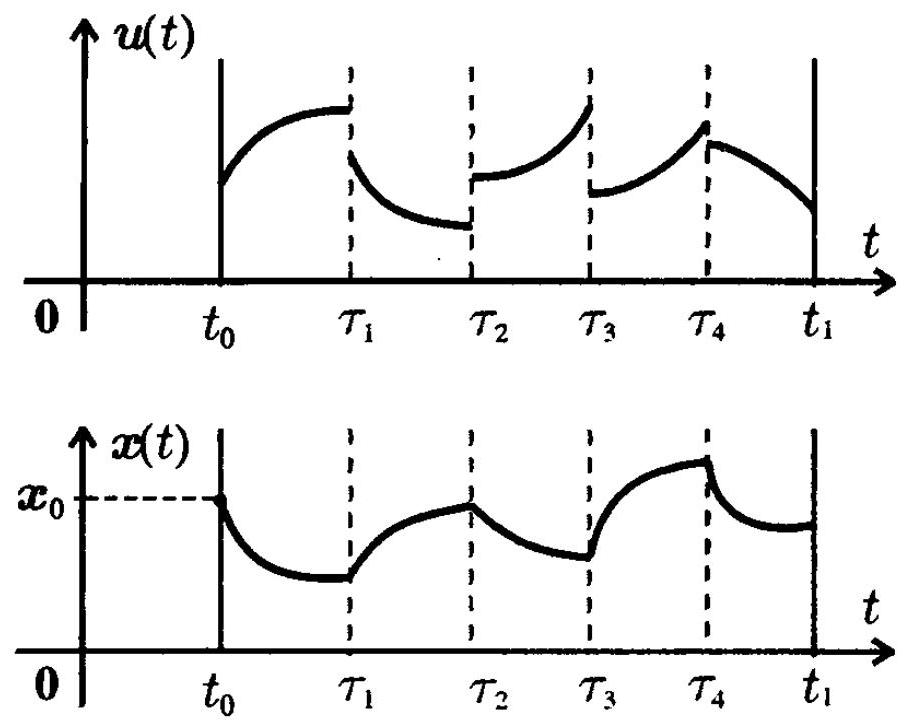
\includegraphics[max width=0.8\textwidth]{images/bo_d547okref24c73bgfch0_78_287_0_910_727_0.jpg}
\end{center}
\hspace*{3em} 

Рис. 19

Функцию \(\mathbf{x}\left( t\right)\) назовем абсолютно непрерывной на отрезке времени \(I = \left[ t_{0},t_{1}\right]\), если ее производная \(\dot{\mathbf{x}}\left( t\right)\) существует для почти всех \(t \in I\), интегрируема по Лебегу и для всех \(t \in I\) выполняется условие

\[
\mathbf{x}\left( t\right)  = \mathbf{x}\left( {t}_{0}\right)  + {\int }_{{t}_{0}}^{t}\dot{\mathbf{x}}\left( s\right) {ds}
\]

т.е. функция \(\mathbf{x}\left( t\right)\) однозначно восстанавливается по своей производной \(\dot{\mathbf{x}}\left( t\right)\). Любая кусочно гладкая функция \(\mathbf{x}\left( t\right)\) является абсолютно непрерывной.

Оказывается, что для любого допустимого управления \(\mathbf{u}\left( t\right)\), т.е. интегрируемой по Лебегу функции \(\mathbf{u}\left( t\right)\), и любого начального состояния \(\mathbf{x}\left( t_{0}\right) = \mathbf{x}_{0}\) можно также определить решение \(\mathbf{x}\left( t\right)\) дифференциального уравнения (6.1). Но в этом случае решение \(\mathbf{x}\left( t\right)\) уже не будет функцией непрерывно дифференцируемой, а будет лишь функцией абсолютно непрерывной.

Можно представить себе, что на рис. 19 число скачков у функции \(\mathbf{u}\left( t\right)\) увеличивается и становится даже счетным. При этом у решения \(\mathbf{x}\left( t\right)\) появится много изломов, т.е. скачков производной \(\dot{\mathbf{x}}\left( t\right)\), хотя само решение \(\mathbf{x}\left( t\right)\) остается абсолютно непрерывным.

Теорема 1. Пусть функция \(\mathbf{u}\left( t\right)\) измерима по Лебегу на отрезке \(I = \left[ t_{0},t_{1}\right]\). Тогда для любого начального значения \(\mathbf{x}\left( t_{0}\right) = \mathbf{x}_{0}\) абсолютно непрерывное решение \(\mathbf{x}\left( t\right)\) уравнения (6.1) существует, является единственным и для любого \(t \in I\) задается формулой Коши (6.7), причем интеграл в этой формуле понимается в смысле Лебега.

Доказательство. Непосредственно проверяется, что функция \(\mathbf{x}\left( t\right)\), задаваемая формулой (6.7), является решением дифференциального уравнения (6.1). Действительно, при \(t = t_{0}\) очевидно выполняется начальное условие \(\mathbf{x}\left( t_{0}\right) = \mathbf{x}_{0}\). Далее, используя свойства экспоненциала, найдем производную функции \(\mathbf{x}\left( t\right)\)

\[
\dot{x}\left( t\right)  = A{e}^{\left( {t - {t}_{0}}\right) A}{x}_{0} + u\left( t\right)  + {\int }_{{t}_{0}}^{t}A{e}^{\left( {t - s}\right) A}u\left( s\right) {ds} =
\]

\[
= A\left\lbrack  {{e}^{\left( {t - {t}_{0}}\right) A}{x}_{0} + {\int }_{{t}_{0}}^{t}{e}^{\left( {t - s}\right) A}u\left( s\right) {ds}}\right\rbrack   + u\left( t\right)  = {Ax}\left( t\right)  + u\left( t\right) .
\]

Видно, что она совпадает с правой частью уравнения (6.1). Таким образом, при подстановке функции \(\mathbf{x}\left( t\right)\) в уравнение (6.1) получаем равенство

\[
\dot{\mathbf{x}}\left( t\right)  = A\mathbf{x}\left( t\right)  + \mathbf{u}\left( t\right) . \tag{6.8}
\]

Заметим, что полученное равенство выполняется лишь для почти всех \(t \in \left[ t_{0},t_{1}\right]\), так как производная \(\dot{\mathbf{x}}\left( t\right)\) абсолютно непрерывной функции \(\mathbf{x}\left( t\right)\) существует лишь почти всюду. Классическое непрерывно дифференцируемое решение \(\mathbf{x}\left( t\right)\) обращает уравнение в тождество при всех \(t\). Тем не менее, абсолютно непрерывная функция \(\mathbf{x}\left( t\right)\) называется решением дифференциального уравнения (6.1), если равенство (6.8) выполняется для почти всех \(t \in \left[ t_{0},t_{1}\right]\). Если изменить управление \(\mathbf{u}\left( t\right)\) в отдельных точках или даже на множестве нулевой меры, то равенство (6.8) сохранится, и функция \(\mathbf{x}\left( t\right)\) останется решением. Она вообще не изменится, так как функция \(\mathbf{u}\left( t\right)\) в формуле (6.7) стоит под знаком интеграла, а интеграл Лебега не меняется, если подынтегральную функцию изменить на множестве нулевой меры.

Осталось доказать единственность решения \(\mathbf{x}\left( t\right)\). Предположим противное, т.е. существуют два различных абсолютно непрерывных решения \(\mathbf{x}\left( t\right)\) и \(\mathbf{y}\left( t\right)\) с одним и тем же начальным условием \(\mathbf{x}\left( t_{0}\right) = \mathbf{y}\left( t_{0}\right) = \mathbf{x}_{0}\). Пусть \(\tau\) -- первый такой момент времени, после которого решения \(\mathbf{x}\left( t\right)\) и \(\mathbf{y}\left( t\right)\) расходятся (рис. 20). Выберем малое число \(\varepsilon > 0\) такое, что \(\varepsilon \|A\| < 1\), и на отрезке времени \(\left[ \tau,\tau + \varepsilon \right]\) рассмотрим функцию \(\mathbf{z}\left( t\right) = \mathbf{x}\left( t\right) - \mathbf{y}\left( t\right)\). Поскольку \(\mathbf{x}\left( t\right)\) и \(\mathbf{y}\left( t\right)\) удовлетворяют равенству (6.8), для функции \(\mathbf{z}\left( t\right)\) получаем соотношение

\[
\dot{z}\left( t\right)  = \dot{x}\left( t\right)  - \dot{y}\left( t\right)  = {Ax}\left( t\right)  - {Ay}\left( t\right)  = A\left( {x\left( t\right)  - y\left( t\right) }\right)  = {Az}\left( t\right)
\]

\begin{center}
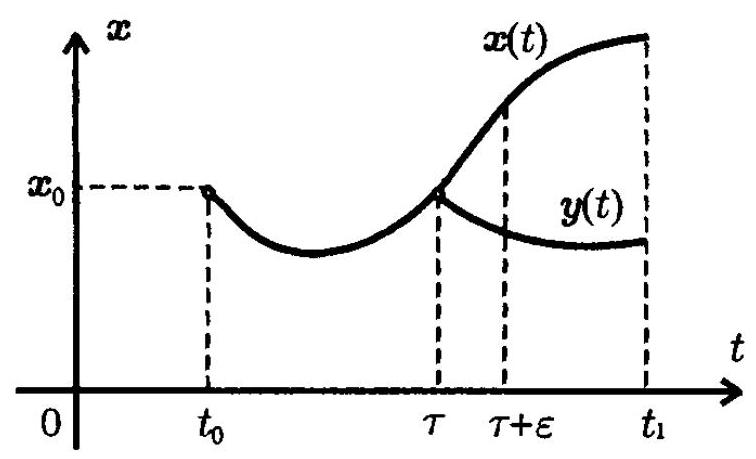
\includegraphics[max width=0.7\textwidth]{images/bo_d547okref24c73bgfch0_80_694_4_756_459_0.jpg}
\end{center}
\hspace*{3em} 

Рис. 20

для почти всех t ∈ \(\left\lbrack  {\tau ,\tau  + \varepsilon }\right\rbrack\) . Проинтегрировав его на отрезке \(\left\lbrack  {\tau ,t}\right\rbrack\) , noлучим равенство

\[
z\left( t\right)  = {\int }_{\tau }^{t}{Az}\left( s\right) {ds}
\]

так как \(z\left( \tau \right)  = 0\) . Таким образом, при всех т < é t < τ + ε справедливо соотношение

\[
\parallel z\left( t\right) \parallel  = \left\lVert \begin{array}{c} {{\int }_{\tau }^{t}{Az}\left( s\right) {ds}} \end{array} \right\rVert \leq  {\int }_{\tau }^{t}\parallel {Az}\left( s\right) \parallel {ds} \leq
\]

\[
\leq  {\int }_{\tau }^{t}\parallel A\parallel  \cdot  \parallel z\left( s\right) \parallel {ds} \leq  \varepsilon  \cdot  \parallel A\parallel \mathop{\max }\limits_{{\tau  \leq  t \leq  \tau  + \varepsilon }}\parallel z\left( t\right) \parallel  < \mathop{\max }\limits_{{\tau  \leq  t \leq  \tau  + \varepsilon }}\parallel z\left( t\right) \parallel .
\]

Поскольку функция \(z\left( t\right)\) непрерывна на отрезке [т, т+ε], она достигает своего максимума в некоторой точке \({t}^{ * } \in  \left\lbrack  {\tau ,\tau  + \varepsilon }\right\rbrack\) . Подставляя в полученное соотношение точку \(t = {t}^{ * }\) ,получим противоречивое неравенство

\[
\left\lVert \begin{array}{c} {\mathbf{z}\left( {t}^{ * }\right) } \end{array} \right\rVert < \left\lVert \begin{array}{c} {\mathbf{z}\left( {t}^{ * }\right) } \end{array} \right\rVert.
\]

Тем самым единственность решения х(t) установлена. Теорема доказана.

Замечание. В теореме 1 начальное условие для решения \(\mathbf{x}\left( t\right)\) уравнения (6.1) задавалось на левом конце отрезка времени \(\left\lbrack  {{t}_{0},{t}_{1}}\right\rbrack\) , т.е. в точке б, и хе и ум решение х(t) задавалось формулой Коши (6.7). Нетрудно проверить, что теорема 1 со- хранится, если задавать начальное условие на правом конце отрезка \(\left\lbrack  {{t}_{0},{t}_{1}}\right\rbrack\) , т.е. в точке \({t}_{1},x\left( {t}_{1}\right)  = {x}_{1}\) . Таким образом, в этом случае решение существует, является единственным и опять задается формулой Коши

\[
\mathbf{x}\left( t\right)  = {e}^{\left( {t - {t}_{1}}\right) A}{\mathbf{x}}_{1} + {\int }_{{t}_{1}}^{t}{e}^{\left( {t - s}\right) A}\mathbf{u}\left( s\right) {ds}. \tag{6.9}
\]

Это все проверяется точно так же, как и при доказательстве теоремы 1 (читателям предлагается выполнить это самостоя- тельно).

Пример 4. Пусть \(n = 2\) . Найти решение системы уравнений

\[
\dot{\mathbf{x}} = \mathbf{u}\left( t\right) ,
\]

гле функпия \(\mathbf{u}\left( t\right)\) задается формулой

\[
u\left( t\right)  = \left\{  \begin{array}{lll} \left( {1,1}\right) , & \mathrm{{\text{ е }\text{ с }\text{ л }\text{ и }}} & 0 \leq  t \leq  1, \\  \left( {1, - 1}\right) , & \mathrm{{\text{ е }\text{ с }\text{ л }\text{ и }}} & 1 < t \leq  2, \end{array}\right.
\]

c начальным условием x0 = x0 = (1,1) на отрезке времени \(\left\lbrack  {0,2}\right\rbrack\) .

B данном случае \(A = 0\) , Cледовательно, \({e}^{tA} = E\) (см. при- мер 1) и формула Коши (6.7) принимает вид

\[
\mathbf{x}\left( t\right)  = {\mathbf{x}}_{0} + {\int }_{{t}_{0}}^{t}\mathbf{u}\left( s\right) {ds}.
\]

Интегрируя функцию \(\mathbf{u}\left( t\right)\) ,получаем решение

\[
x\left( t\right)  = \left\{  \begin{array}{lll} \left( {1 + t,1 + t}\right) , & \operatorname{ec\text{ л }\text{ и }} & 0 \leq  t \leq  1, \\  \left( {1 + t,3 - t}\right) , & \operatorname{ec\text{ л }\text{ и }} & 1 < t \leq  2. \end{array}\right.
\]

Это решение кусочно гладко, его производная имеет разрыв в точке t = 1. На рис. 21 это решение изображено в фазовой плоскости переменного \(\mathbf{x} = \left( {{\mathbf{x}}^{1},{\mathbf{x}}^{2}}\right)  \in  {E}^{2}\) .

\[
\left\{  \begin{array}{l} {\dot{x}}^{1} = {x}^{2} + {u}^{1}\left( t\right) \\  {\dot{x}}^{2} =  - {x}^{1} + {u}^{2}\left( t\right)  \end{array}\right. \tag{6.10}
\]

\begin{center}
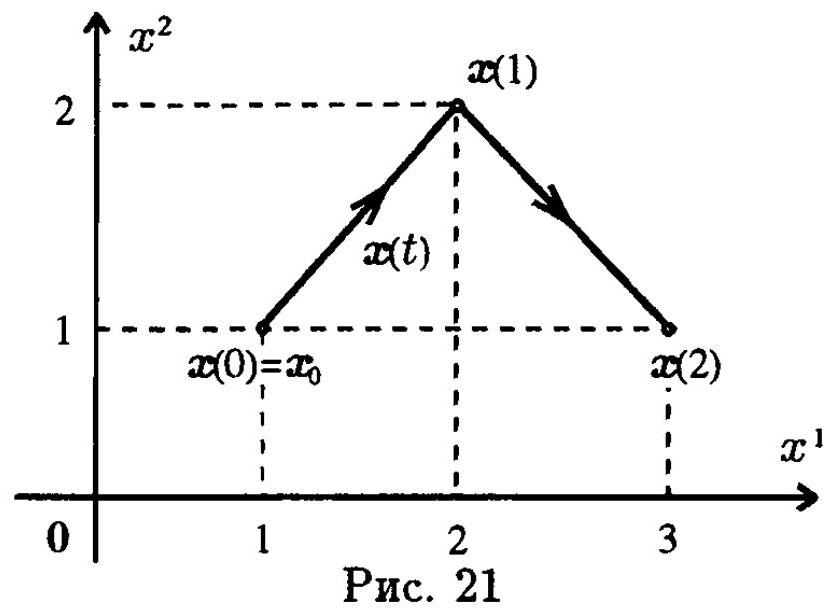
\includegraphics[max width=0.8\textwidth]{images/bo_d547okref24c73bgfch0_82_313_0_835_615_0.jpg}
\end{center}
\hspace*{3em} 

Пример 5. Найти решение системы дифференциальных уравнений

c начальным условием x0 = (1,0), когда функция u(t) кусочно непрерывна и задана на отрезке времени [0, π] условием

\[
\mathbf{u}\left( t\right)  = \left( {{u}^{1}\left( t\right) ,{u}^{2}\left( t\right) }\right)  = \left\{  \begin{array}{lll} \left( {0,1}\right) , & \mathrm{{\text{ е }\text{ с }\text{ л }\text{ и }}} & 0 \leq  t \leq  \frac{\pi }{2}, \\  \left( {-1,0}\right) , & \mathrm{{\text{ е }\text{ с }\text{ л }\text{ и }}} & \frac{\pi }{2} < t \leq  \pi . \end{array}\right.
\]

Для уравнения (6.10) имеем \(A = \left( \begin{array}{cc} 0 & 1 \\   - 1 & 0 \end{array}\right)\) . Экспоненциал этой матрицы уже вычислен в примере 2 и равняется

\[
{e}^{tA} = \left( \begin{array}{cc} \cos t & \sin t \\   - \sin t & \cos t \end{array}\right) .
\]

Подставляя это выражение, а также начальное условие но = 0, \(\mathbf{x}\left( 0\right)  = \left( {1,0}\right)\) и функцию \(\mathbf{u}\left( t\right)\) в формулу Коши, для всех t ∈ \(\left\lbrack  {0,\frac{\pi }{2}}\right\rbrack\) получаем решение

\[
\mathbf{x}\left( t\right)  = \left( \begin{array}{cc} \cos t & \sin t \\   - \sin t & \cos t \end{array}\right) \left( \begin{array}{l} 1 \\  0 \end{array}\right)  +
\]

\[
+ {\int }_{0}^{t}\left( \begin{array}{cc} \cos \left( {t - s}\right) & \sin \left( {t - s}\right) \\   - \sin \left( {t - s}\right) & \cos \left( {t - s}\right) \end{array}\right) \left( \begin{array}{l} 0 \\  1 \end{array}\right) {ds} =
\]

\[
= \left( \begin{array}{c} \cos t \\   - \sin t \end{array}\right)  + {\int }_{0}^{t}\left( \begin{array}{c} \sin \left( {t - s}\right) \\  \cos \left( {t - s}\right) \end{array}\right) {ds} =
\]

\[
= \left( \begin{array}{c} \cos t \\   - \sin t \end{array}\right)  + \left( \begin{array}{c} 1 - \cos t \\  \sin t \end{array}\right)  = \left( \begin{array}{l} 1 \\  0 \end{array}\right) .
\]

Аналогичным образом для \(t \in  \left\lbrack  {\frac{\pi }{2},\pi }\right\rbrack\) ,подставив в формулу Коши (6.7) функцию \(\mathbf{u}\left( t\right)\) и начальное условие x( \(\frac{\pi }{2}\) ) = (1,0),получаем решение

\[
\mathbf{x}\left( t\right)  = \left( \begin{array}{cc} \cos \left( {t - \frac{\pi }{2}}\right) & \sin \left( {t - \frac{\pi }{2}}\right) \\   - \sin \left( {t - \frac{\pi }{2}}\right) & \cos \left( {t - \frac{\pi }{2}}\right) \end{array}\right) \left( \begin{array}{l} 1 \\  0 \end{array}\right)  +
\]

\[
+ {\int }_{\frac{\pi }{2}}^{t}\left( \begin{array}{cc} \cos \left( {t - s}\right) & \sin \left( {t - s}\right) \\   - \sin \left( {t - s}\right) & \cos \left( {t - s}\right) \end{array}\right) \left( \begin{array}{c} - 1 \\  0 \end{array}\right) {ds} =
\]

\[
= \left( \begin{array}{c} \cos \left( {t - \frac{\pi }{2}}\right) \\   - \sin \left( {t - \frac{\pi }{2}}\right) \end{array}\right)  + {\int }_{\frac{\pi }{2}}^{t}\left( \begin{array}{c} - \cos \left( {t - s}\right) \\  \sin \left( {t - s}\right) \end{array}\right) {ds} =
\]

\[
= \left( \begin{array}{c} \sin t \\   - \cos t \end{array}\right)  + \left( \begin{array}{c} \cos t \\  1 - \sin t \end{array}\right)  = \left( \begin{array}{c} \sin t + \cos t \\  1 + \cos t - \sin t \end{array}\right) .
\]

Окончательно имеем решение

\[
\mathbf{x}\left( t\right)  = \left\{  \begin{array}{lll} \left( {1,0}\right) , & \operatorname{ec\text{ л }\text{ и }} & 0 \leq  t \leq  \frac{\pi }{2}, \\  \left( {\sin t + \cos t,1 + \cos t - \sin t}\right) , & \operatorname{ec\text{ л }\text{ и }} & \frac{\pi }{2} < t \leq  \pi . \end{array}\right.
\]

Это решение является абсо- лютно непрерывной функци- ей, оно кусочно гладко, но не является функцией непрерыв- но дифференцируемой. Его производная \(\dot{x}\left( t\right)\) имеет раз- рыв при \(t = \frac{\pi }{2}\) . На рис. 22 ре- шение \(x\left( t\right)\) изображено в фа- зовой плоскости \(\left( {{x}^{1},{x}^{2}}\right)  \in  {E}^{2}\) .

\begin{center}
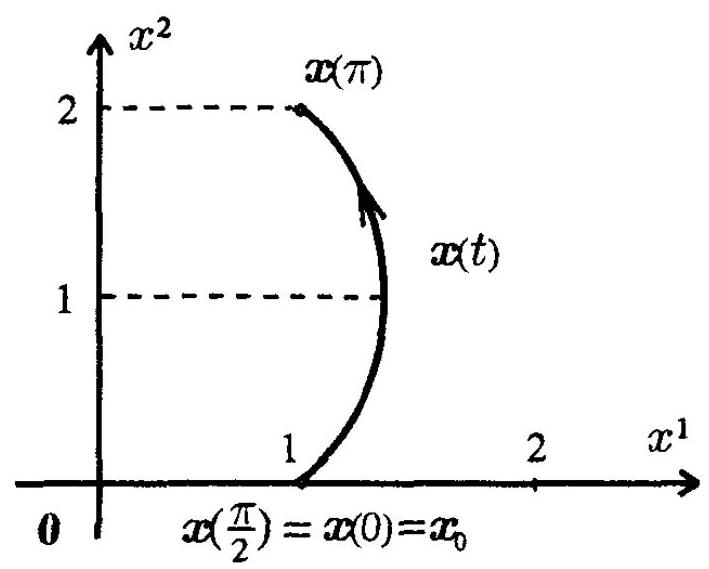
\includegraphics[max width=0.6\textwidth]{images/bo_d547okref24c73bgfch0_83_11_1509_709_569_0.jpg}
\end{center}
\hspace*{3em} 

Pnc. 22

Пример 6. Найти решение системы дифференциальных уравнений

\[
\left\{  \begin{array}{l} {\dot{x}}^{1} = {x}^{2} \\  {\dot{x}}^{2} = {u}^{2} \end{array}\right.
\]

с начальным условием на правом конце отрезка времени [0,2], \(\mathbf{x}\left( 2\right)  = \mathbf{0}\) ,когда функция \(\mathbf{u}\left( t\right)\) кусочно непрерывна и задана условием

\[
\mathbf{u}\left( t\right)  = \left( {{u}^{1}\left( t\right) ,{u}^{2}\left( t\right) }\right)  = \left\{  \begin{array}{lll} \left( {0,0}\right) , & \operatorname{ec\text{ л }\text{ и }} & 0 \leq  t \leq  1, \\  \left( {0,1}\right) , & \operatorname{ec\text{ л }\text{ и }} & 1 < t \leq  2. \end{array}\right.
\]

Экспоненциал матрицы \(A = \left( \begin{array}{ll} 0 & 1 \\  0 & 0 \end{array}\right)\) вычислен в примере 3. Он имеет вид

\[
{e}^{tA} = \left( \begin{array}{ll} 1 & t \\  0 & 1 \end{array}\right)
\]

Подставив это выражение и условие х0(2) = 0 в формулу (6.9), получим выражение

\[
x\left( t\right)  = {\int }_{0}^{t}\left( \begin{array}{cc} 1 & t - s \\  0 & 1 \end{array}\right) \left( \begin{array}{c} {u}^{1}\left( s\right) \\  {u}^{2}\left( s\right) \end{array}\right) {ds}.
\]

Подставив сюда функцию \(\mathbf{u}\left( t\right)\) и проинтегрировав, получаем

\[
x\left( t\right)  = \left( {\frac{{t}^{2}}{2} - {2t} + 2,t - 2}\right)
\]

\begin{center}
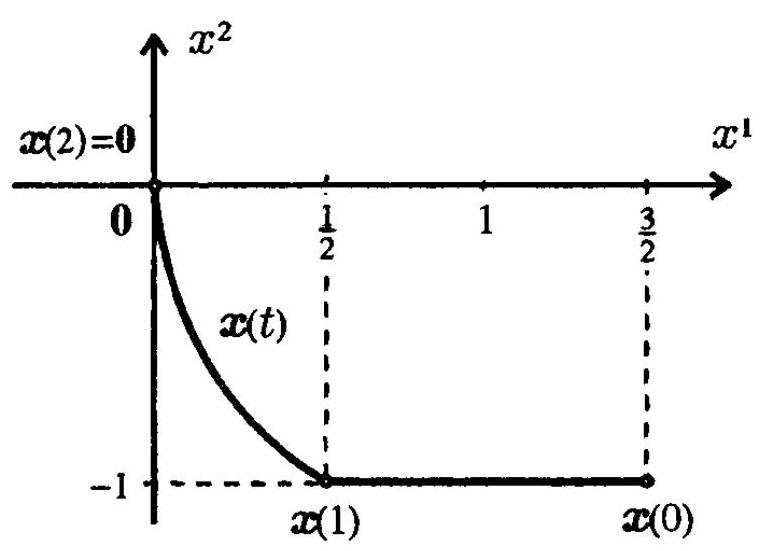
\includegraphics[max width=0.7\textwidth]{images/bo_d547okref24c73bgfch0_84_702_1406_761_551_0.jpg}
\end{center}
\hspace*{3em} 

Рис. 23

при \(1 < t \leq  2\) и

\[
x\left( t\right)  = \left( {-t + \frac{3}{2}, - 1}\right)
\]

при \(0 \leq  t \leq  1\) .

Ha puc.23это решение изображено в фазовой плос- кости \(\left( {{x}^{1},{x}^{2}}\right)  \in  {E}^{2}\) .

\section*{6.4. Задачи}

1. Пусть A и B — произвольные матрицы размером n × n. Всегда ли выполняется равенство

\[
{e}^{A} \cdot  {e}^{B} = {e}^{A + B}?
\]

2. Вычислите экспоненциал \({e}^{tA}\) для следующих матриц A:

1) \(\left( \begin{array}{cc} 0 & 1 \\  0 &  - 1 \end{array}\right)\) , 2) \(\left( \begin{array}{ll} 0 & 1 \\  1 & 0 \end{array}\right)\) ,

3) \(\left( \begin{array}{lll} 0 & 1 & 0 \\  0 & 0 & 1 \\  0 & 0 & 0 \end{array}\right)\) , 4) \(\left( \begin{array}{lll} 0 & 0 & 1 \\  0 & 1 & 0 \\  1 & 0 & 0 \end{array}\right)\) ,

5) \(\left( \begin{array}{ccccc} 0 & 1 & 0 & \cdots & 0 \\  0 & 0 & 1 & \cdots & 0 \\   - &  - &  - &  - &  - \\  0 & 0 & 0 & \cdots & 1 \\  0 & 0 & 0 & \cdots & 0 \end{array}\right)\) , 6) \(\left( \begin{array}{ccccc} \lambda & 1 & 0 & \cdots & 0 \\  0 & \lambda & 1 & \cdots & 0 \\   - &  - &  - &  - & \\  0 & 0 & \lambda & \cdots & 1 \\  0 & 0 & 0 & \cdots & \lambda \end{array}\right)\) .

3. Вычислите экспоненциал блочной матрицы

\[
\left( \begin{array}{ccccccccc} {A}_{1} &  \parallel  & 0 &  \parallel  & 0 &  \parallel  & \ldots &  \parallel  & 0 \\   - &  - &  - &  - &  - &  - &  - &  - &  - \\  0 &  \parallel  & {A}_{2} &  \parallel  & 0 &  \parallel  & \ldots &  \parallel  & 0 \\   - &  - &  - &  - &  - &  - &  - &  - &  - \\  \vdots &  \parallel  & \vdots &  \parallel  & \vdots &  \parallel  &  \ddots  &  \parallel  & \vdots \\   - &  - &  - &  - &  - &  - &  - &  - &  - \\  0 &  \parallel  & 0 &  \parallel  & 0 &  \parallel  & \ldots &  \parallel  & {A}_{n} \end{array}\right) .
\]

4. Докажите, что если матрица \(A\) имеет вид \(A = {T}^{-1}{BT}\) , где \(T -\) невырожденное преобразование, то

\[
{e}^{tA} = {T}^{-1}{e}^{tB}T
\]

\section*{лекция 7}

\begin{itemize}\relax
\item\relax Множества достижимости и управляемости ли- нейной управляемой системы.
\end{itemize}

\begin{itemize}\relax
\item\relax Их основные свойства.
\end{itemize}

\section*{7.1. Множество достижимости}

Рассмотрим снова управляемый объект, поведение которого описывается линейной системой дифференциальных уравнений

\[
\dot{\mathbf{x}} = A\mathbf{x} + \mathbf{u}, \tag{7.1}
\]

класс допустимых управлений, состоящий из всех функций \(\mathbf{u}\left( t\right) \in U\), \(U \in \Omega \left( {E}^{n}\right)\), интегрируемых по Лебегу на отрезке времени \(I = \left[ t_{0},t_{1}\right]\), и начальное множество \(M_{0} \in \Omega \left( {E}^{n}\right)\). Пусть \(t \in \left[ t_{0},t_{1}\right]\). Множеством достижимости \(X(t)\) в момент времени \(t\) назовем множество всех точек из фазового пространства \(E^{n}\), в которые можно перейти на отрезке времени \(\left[ t_{0},t_{1}\right]\) из всех возможных точек начального множества \(M_{0}\) по решениям уравнения (7.1) при всех возможных допустимых управлениях \(\mathbf{u}(t)\). Таким образом, множество достижимости \(X(t)\) состоит из всех точек вида \(\mathbf{x}(t)\), где \(\mathbf{x}(t)\) -- решение уравнения (7.1) с начальным условием \(\mathbf{x}\left( t_{0}\right) \in M_{0}\) и с допустимым управлением \(\mathbf{u}(t)\) (рис. 24). Множество достижимости зависит, конечно, от матрицы \(A\), ограничивающего множества \(U\), множества начальных состояний \(M_{0}\) и отрезка времени \(\left[ t_{0},t\right]\). Рассмотрим некоторые свойства множества достижимости.

Свойство 1. Множество достижимости X(t) представ- ляется в виде

\[
X\left( t\right)  = {e}^{\left( {t - {t}_{0}}\right) A}{M}_{0} + {\int }_{{t}_{0}}^{t}{e}^{\left( {t - s}\right) A}{Uds}, \tag{7.2}
\]

где е вене мета мета метества Мо при линейном преобра- зовании \({e}^{\left( {t - {t}_{0}}\right) A}\) (см. лекцию 2), а под знаком интеграла сто- ит многозначное отображение, которое получается для всех \(s \in  \left\lbrack  {{t}_{0},t}\right\rbrack\) как образ множества U при линейном преобразова- нии \({e}^{\left( {t - s}\right) A}\) .

\begin{center}
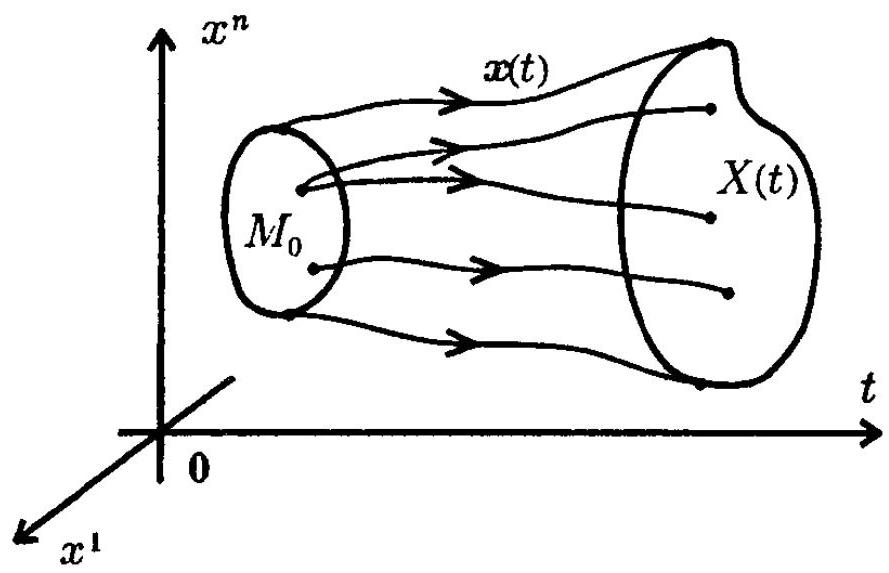
\includegraphics[max width=0.8\textwidth]{images/bo_d547okref24c73bgfch0_87_293_0_889_573_0.jpg}
\end{center}
\hspace*{3em} 

Рис. 24

Доказательство свойства 1 непосредственно следует из формулы Коши

\[
\mathbf{x}\left( t\right)  = {e}^{\left( {t - s}\right) A}\mathbf{x}\left( {t}_{0}\right)  + {\int }_{{t}_{0}}^{t}{e}^{\left( {t - s}\right) A}\mathbf{u}\left( s\right) {ds}
\]

(см. лекцию 6) и определений множества достижимости, образа множества при линейном преобразовании, алгебраической сум- мы множеств (см. лекцию 2) и интеграла Лебега от многознач- ного отображения (см. лекцию 5).

Свойство 2. Множество достижимости является не- пустым компактным подмножеством фазового пространст- \({\text{ в }\text{ а }}{E}^{n},\) т.е. \(X\left( t\right)  \in  \Omega \left( {E}^{n}\right) .\)

Доказательство этого свойства непосредственно следу- ет из формулы (7.2) и теоремы 1 о непустоте и компактности интеграла от многозначного отображения (см. лекцию 5).

Свойство 3. Если начальное множество М0 выпукло, то множество достижимости \(X\left( t\right)\) тоже выпукло.

Доказательство этого свойства очевидным образом сле- дует из формулы (7.2) и теоремы 1 о выпуклости интеграла от многозначного отображения (см. лекцию 5).

Свойство 4. Опорная функция множества достижимости имеет вид

\[
c\left( {X\left( t\right) ,\psi }\right)  = c\left( {{M}_{0},{e}^{\left( {t - {t}_{0}}\right) {A}^{ * }}\psi }\right)  + {\int }_{{t}_{0}}^{t}c\left( {U,{e}^{\left( {t - s}\right) {A}^{ * }}\psi }\right) {ds}. \tag{7.3}
\]

Доказательство этого свойства также непосредственно следует из формулы (7.2), свойств опорных функций и теоремы 2 (см. лекцию 5).

Действительно, если взять опорную функцию от левой и пра- вой частей равенства (7.2) и воспользоваться перечисленными фактами, то получим формулу (7.3).

Свойство 5. Пусть т — длина отрезка времени [t, t], т.е. \(\tau  = t - {t}_{0}\) . Toгда множество достижимости X(t) зависит только от длины отрезка τ и имеет вид

\[
X\left( t\right)  = {e}^{\tau A}{M}_{0} + {\int }_{0}^{\tau }{e}^{sA}{Uds} \tag{7.4}
\]

Доказательство. Заметим, что для каждого конкретного управления \(\mathbf{u}\left( t\right)  \in  U\) дифференциальное уравнение (7.1) не яв- ляется автономным, но поскольку ограничивающее множество \(U\) постоянно, управляемый объект

\[
\dot{\mathbf{x}} = A\mathbf{x} + \mathbf{u},\;\mathbf{u} \in  U
\]

в целом ведет себя как автономная система дифференциальных уравнений. При этом неважно, в какой момент времени и на- чать движение, множество достижимости \(X\left( t\right)\) зависит толь- ко от длины временнóго интервала т = t - s. Сделав замену переменных \(t - s = \alpha\) в интеграле в формуле (7.3), noлучаем равенства

\[
{\int }_{{t}_{0}}^{t}c\left( {U,{e}^{\left( {t - s}\right) {A}^{ * }}\psi }\right) {ds} = {\int }_{t - {t}_{0}}^{0}c\left( {U,{e}^{\alpha {A}^{ * }}\psi }\right) \left( {-{d\alpha }}\right)  = {\int }_{0}^{t - {t}_{0}}c\left( {U,{e}^{\alpha {A}^{ * }}\psi }\right) {d\alpha }.
\]

(7.5)

Восстановив теперь по этим опорным функциям выпуклые ком- пактные множества, получим равенство

\[
{\int }_{{t}_{0}}^{t}{e}^{\left( {t - s}\right) A}{Uds} = {\int }_{0}^{t - {t}_{0}}{e}^{\alpha A}{Ud\alpha }
\]

Учитывая, что \(\tau  = t - {t}_{0}\) ,и формулу (7.2), получаем форму- лу (7.4).

Свойство 6. Опорная функция \(c\left( {X\left( t\right) ,\psi }\right)\) как функция дли- ны отрезка \(\tau  = t - {t}_{0}\) имеет вид

\[
c\left( {X\left( t\right) ,\psi }\right)  = c\left( {{M}_{0},{e}^{\tau {A}^{ * }}\psi }\right)  + {\int }_{0}^{\tau }c\left( {U,{e}^{s{A}^{ * }}\psi }\right) {ds}. \tag{7.6}
\]

Доказательство этой формулы очевидно. Для этого нуж- но либо во всей формуле (7.3) сделать замену переменной, либо просто взять опорную функцию от левой и правой частей в фор- муле (7.4).

Свойство 7. Множество достижимости Х(t) непрерыв- но зависит от аргумента t, т.е. многозначное отображение \(X\left( \cdot \right)  : I \rightarrow  \Omega \left( {E}^{n}\right)\) непрерывно в метрике Хаусдорфа.

Доказательство. Согласно формуле (7.4) множество достижимости \(X\left( t\right)\) непрерывно зависит от длины отрезка \(\tau = t - {t}_{0}\). Действительно, в силу теоремы 3 (см. лекцию 5), интеграл от многозначного отображения непрерывен по верхнему пределу, а отображение \({e}^{\tau A}M_{0}\) непрерывно как образ постоянного множества \(M_{0}\) при непрерывном линейном преобразовании \({e}^{\tau A}\) (см. лекцию 4). Следовательно, отображение \(X\left( t\right)\) непрерывно зависит от \(\tau\) как сумма двух непрерывных многозначных отображений. Если начальный момент времени \(t_{0}\) фиксирован, то множество достижимости \(X\left( t\right)\) непрерывно зависит от аргумента \(t = {t}_{0} + \tau\).

Множества достижимости играют фундаментальную роль в теории оптимального управления. На их свойствах основаны все дальнейшие результаты. Для этих свойств существенно то, что в качестве класса допустимых управлений выбирают все- возможные измеримые функции \(\mathbf{u}\left( t\right)  \in  U\) , т.е. функции, интег- рируемые по Лебегу на любом конечном отрезке времени [и, н2]. Именно в этом классе функций интеграл от многозначного ото- бражения, а следовательно, и множество достижимости являет- ся непустым, выпуклым и компактным.

\section*{7.2. Множество управляемости}

Рассмотрим, помимо множества достижимости X(t), еще од- но множество — множество управляемости \(Y\left( t\right)\) . Множеством управляемости \(Y\left( t\right)\) в любой момент времени t ∈ \(\left\lbrack  {{t}_{0},{t}_{1}}\right\rbrack\) называ- ют множество всех точек фазового пространства E", из которых можно перейти на отрезке времени [t, t] на множество конечных состояний \({M}_{1}\) по решениям уравнения (7.1) при всевозможных допустимых управлениях и (1) ∈ U (puc. 25). Таким образом, множество управляемости \(Y\left( t\right)\) состоит из всех точек \{x(t)\}, где \(\mathbf{x}\left( t\right)\) — решение уравнения (7.1) с условием на правом конце \(\mathbf{x}\left( {t}_{1}\right)  \in  {M}_{1}\) и с допустимым управлением и(t).

Поскольку каждое такое решение также задается формулой Komm (см. формулу (6.9) лекиий 6)

\[
\mathbf{x}\left( t\right)  = {e}^{\left( {t - {t}_{1}}\right) A}\mathbf{x}\left( {t}_{1}\right)  + {\int }_{{t}_{1}}^{t}{e}^{\left( {t - s}\right) A}\mathbf{u}\left( s\right) {ds} =
\]

\[
= {e}^{\left( {t - {t}_{1}}\right) A}x\left( {t}_{1}\right)  + {\int }_{t}^{t}{e}^{\left( {t - s}\right) A}\left\lbrack  {-u\left( s\right) }\right\rbrack  {ds},
\]

множество управляемости имеет вид

\[
Y\left( t\right)  = {e}^{\left( {t - {t}_{1}}\right) A}{M}_{1} + {\int }_{t}^{{t}_{1}}{e}^{\left( {t - s}\right) A}\left\lbrack  {-U}\right\rbrack  {ds}. \tag{7.7}
\]

Точно так же доказывается, что множество управляемости не- пусто и компактно, оно выпукло, если выпукло множество М1, и непрерывно зависит от времени t. Опорная функция множества управляемости \(Y\left( t\right)\) имеет вид

\[
c\left( {Y\left( t\right) ,\psi }\right)  = c\left( {{M}_{1},{e}^{\left( {t - {t}_{1}}\right) {A}^{ * }}\psi }\right)  + {\int }_{t}^{{t}_{1}}c\left( {U, - {e}^{\left( {t - s}\right) {A}^{ * }}\psi }\right) {ds}. \tag{7.8}
\]

\begin{center}
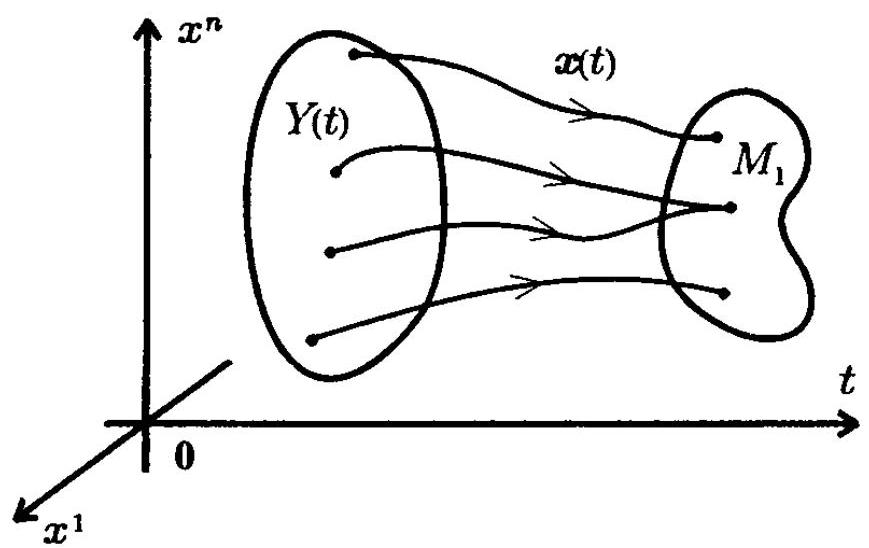
\includegraphics[max width=0.8\textwidth]{images/bo_d547okref24c73bgfch0_90_288_1573_869_548_0.jpg}
\end{center}
\hspace*{3em} 

Рис. 25

Пусть \(\tau\) - длина отрезка времени \(\left\lbrack  {t,{t}_{1}}\right\rbrack\) , т.е. \(\tau  = {t}_{1} - t\) . Тогда множество управляемости \(Y\left( t\right)\) зависит только от длины отрезка \(\tau\) и имеет вид

\[
Y\left( t\right)  = {e}^{-{\tau A}}{M}_{1} + {\int }_{0}^{\tau }{e}^{-{sA}}\left\lbrack  {-U}\right\rbrack  {ds} \tag{7.9}
\]

а его опорная функция задается формулой

\[
c\left( {Y\left( t\right) ,\psi }\right)  = c\left( {{M}_{1},{e}^{-\tau {A}^{ * }}\psi }\right)  + {\int }_{0}^{\tau }c\left( {U, - {e}^{-s{A}^{ * }}\psi }\right) {ds}. \tag{7.10}
\]

Все эти свойства множества управляемости \(Y\left( t\right)\) проверя- ются точно так же, как это было сделано при доказательстве свойств 1 — 7 множества достижимости X (t).

Заметим, что перечисленные выше свойства множеств до- стижимости и управляемости справедливы для любой матрицы \(A\) и любых непустых компактных множеств U, \({M}_{0},{M}_{1} \in  \Omega \left( {E}^{n}\right)\) , т.е. справедливы для любой линейной управляемой систе- мы (7.1).

Пример 1. Для матрицы \(A = 0\) для множества достижи- мости \(X\left( t\right)\) и множества управляемости \(Y\left( t\right)\) из формул (7.4) и (7.9) получаем соответственно следующие выражения:

\[
X\left( t\right)  = {M}_{0} + {\int }_{0}^{\tau }{Uds} = {M}_{0} + \tau \operatorname{conv}U
\]

\[
Y\left( t\right)  = {M}_{1} + {\int }_{0}^{\tau }\left( {-U}\right) {ds} = {M}_{1} + \tau \operatorname{conv}\left( {-U}\right)
\]

(см. пример 3 об интегрировании постоянного множества из лек- ции 5).

\begin{center}
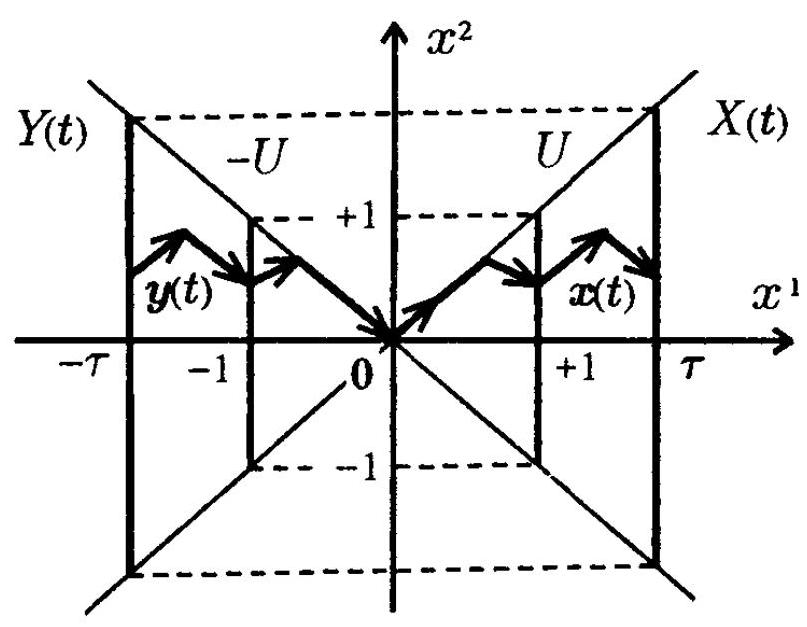
\includegraphics[max width=0.7\textwidth]{images/bo_d547okref24c73bgfch0_92_657_1_807_627_0.jpg}
\end{center}
\hspace*{3em} 

Рис. 26

Пусть, в частности, \(n = 2\) и множество \(U\) co- стоит из двух точек (1,1), \(\left( {1, - 1}\right)\) (рис. 26). Если \({M}_{0} = \{ 0\}\) , ro множество достижимости \(X\left( t\right)\) на лю- бом отрезке времени \(\left\lbrack  {{t}_{0},t}\right\rbrack\) длины \(\tau  = t - {t}_{0}\) ecть отре- 30K

\[
X\left( t\right)  = \left\{  {\mathbf{x} \in  {E}^{2} : }\right.
\]

\[
{x}^{1} = \tau ,\left| {x}^{2}\right|  \leq  \tau \}
\]

Если положить \({M}_{1} = \{ \mathbf{0}\}\) , ro множество управляемости \(Y\left( t\right)\) на любом отрезке времени [t, t] длины т = t, 1 – t есть отрезок

\[
Y\left( t\right)  = \left\{  {x \in  {E}^{2} : {x}^{1} =  - \tau ,\left| {x}^{2}\right|  \leq  \tau }\right\}  .
\]

На рис. 26 приведены также две конкретные траектории. Реше- ние \(x\left( t\right)\) переводит точку \({M}_{0} = \{ \mathbf{0}\}\) в некоторую точку множес- тва \(X\left( t\right)\) на отрезке времени длины \(\tau\) , a peшение \(\mathbf{y}\left( t\right)\) переводит некоторую точку множества \(Y\left( t\right)\) в точку \({M}_{1} = \{ \mathbf{0}\}\) на отрезке времени длины т.

Замечание. При вычислении множества достижимости \(X\left( {t,{M}_{0}}\right)\) из начального множества М0 на отрезке времени \(\tau  = t - {t}_{0}\) основную трудность представляет вычисление мно- жества достижимости из начала координат \({M}_{0} = \{ \mathbf{0}\}\) ,т.е. мно- жества

\[
X\left( {t,\{ 0\} }\right)  = {\int }_{0}^{\tau }{e}^{sA}{Uds} \tag{7.11}
\]

(см. формулу (7.4)). Множество достижимости из произвольного начального множества М0 получаем прибавлением слагаемого \({e}^{\tau A}{M}_{0}\) . Например,если бы состоит из одной начальной точки \(\left\{  {\mathbf{x}}_{0}\right\}\) ,то для каждого \(\tau\) нужно сдвинуть множество \(X\left( {t,\{ \mathbf{0}\} }\right)\) на вектор \({e}^{\tau A}{\mathbf{x}}_{0}\) . Аналогично обстоит дело с множеством управля- emocти \(Y\left( t\right)\) .

Для вычисления множества достижимости X(t) или мно- жества управляемости \(Y\left( t\right)\) , korда множества М0 и М1 выпук- лые, следует сначала вычислить их опорные функции (7.6) или (7.10), a затем восстановить выпуклые компакты \(X\left( t\right)\) или \(Y\left( t\right)\) по их опорным функциям.

Пример 2. Найти множество достижимости \(X\left( t\right)\) при \(0 \leq \; \leq  \tau  \leq  \pi\) из начального множества \({M}_{0} = \{ \mathbf{0}\}\) для управляемой системы, описывающей поведение маятника (см. пример 2 из лекции 1):

\[
\left\{  \begin{array}{l} {\dot{x}}^{1} = {x}^{2} \\  {\dot{x}}^{2} =  - {x}^{1} + v \end{array}\right.
\]

c ограничением на управляющую силу \(\left| {v\left( t\right) }\right|  \leq  1\) .

Чтобы привести эту систему к стандартному виду (7.1), определим вектор управления \(\mathbf{u} = \left( {{u}^{1},{u}^{2}}\right)  = \left( {0,v}\right)\) . Тогда мно- жество \(U\) будет отрезком

\[
U = \left\{  {u \in  {E}^{2} : {u}^{1} = 0,\left| {u}^{2}\right|  \leq  1}\right\}
\]

в фазовом пространстве E2. Его опорная функция, очевидно, имеет вид

\[
c\left( {U,\psi }\right)  = \left| {\psi }^{2}\right| .
\]

Экспоненциал \({e}^{tA}\) для матрицы \(A = \left( \begin{array}{rr} 0 & 1 \\   - 1 & 0 \end{array}\right)\) paccматривае- мой системы уже вычислен в примере 2 (см. лекцию 6):

\[
{e}^{tA} = \left( \begin{array}{rr} \cos t & \sin t \\   - \sin t & \cos t \end{array}\right) .
\]

Найдем теперь опорную функцию множества достижимости \(c\left( {X\left( t\right) ,\psi }\right)\) . Подставив в формулу (7.6) значения \({M}_{0},U\) и \({e}^{tA}\) , после несложных вычислений получаем выражение

\[
c\left( {X\left( t\right) ,\psi }\right)  = {\int }_{0}^{\tau }\left| {{\psi }^{1}\sin s + {\psi }^{2}\cos s}\right| {ds}.
\]

Произвольный вектор \(\psi  = \left( {{\psi }^{1},{\psi }^{2}}\right)  \in  S\) на плоскости \({E}^{2}\) пред- ставим в полярных координатах

\[
{\psi }^{1} = \cos \alpha ,\;{\psi }^{2} = \sin \alpha ,\;0 \leq  \alpha  \leq  {2\pi }. \tag{7.12}
\]

Таким образом, для опорной функции \(c\left( {X\left( t\right) ,\mathbf{\psi }}\right)\) получим выра- жение

\[
c\left( {X\left( t\right) ,\psi }\right)  = {\int }_{0}^{\tau }\left| {\sin \left( {\alpha  + s}\right) }\right| {ds} = {\int }_{\alpha }^{\alpha  + \tau }\left| {\sin \theta }\right| {d\theta }. \tag{7.13}
\]

\begin{center}
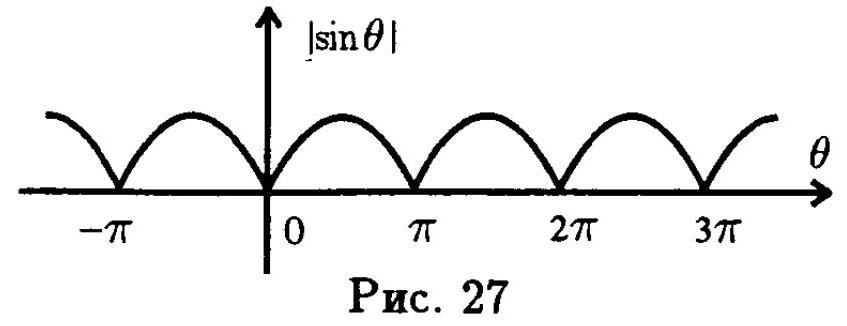
\includegraphics[max width=0.8\textwidth]{images/bo_d547okref24c73bgfch0_94_311_0_847_326_0.jpg}
\end{center}
\hspace*{3em} 

Итак, чтобы научиться вычислять опорную функ- цию, нужно уметь интег- рировать функцию |sinθ| (рис. 27). Эта функция пе- риодическая с периодом \(\pi\) . Интеграл от функции [ sin θ] на отрезке [0, β] тоже пери- одическая функция от па- раметра β с периодом \(\pi\) (рис. 28) и задается форму- non

\[
{\int }_{0}^{\beta }\left| {\sin \theta }\right| {d\theta } = 2\left\lbrack  \frac{\beta }{\pi }\right\rbrack   - 1 - \cos \left( {\beta  - \left\lbrack  \frac{\beta }{\pi }\right\rbrack  \pi }\right) , \tag{7.14}
\]

\begin{center}
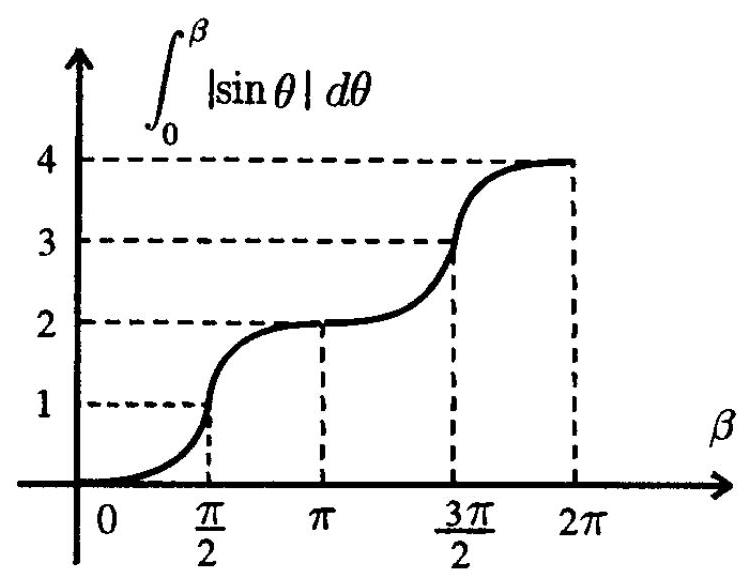
\includegraphics[max width=0.7\textwidth]{images/bo_d547okref24c73bgfch0_94_702_384_745_582_0.jpg}
\end{center}
\hspace*{3em} 

Pac. 28

где [禽] — целая часть числа д. Это несложное упражнение из математического анализа читателям предлагается проделать самостоятельно.

Используя формулу (7.14), вычислим опорную функцию (7.13). Вычисление распадает- ся на четыре случая в зависи- мости от значения параметра \(0 \leq  \alpha  \leq  \pi\) ,точнее,в зависи- мости от того, в какой из че- тырех секторов попадает угол a (puc. 29). Проведя аккуратные вычисления, получаем для опор- ной функции следующее выра- жение:

\[
c\left( {X\left( t\right) ,\psi }\right)  = \begin{cases} \left( {1 - \cos \tau }\right) \cos \alpha  + \sin \tau \sin \alpha , & 0 \leq  \alpha  \leq  \pi  - \tau , \\  2 + \left( {1 + \cos \tau }\right) \cos \alpha  - \sin \tau \sin \alpha , & \pi  - \tau  < \alpha  \leq  \pi , \\  \left( {\cos \tau  - 1}\right) \cos \alpha  - \sin \tau \sin \alpha , & \pi  < \alpha  \leq  {2\pi } - \tau , \\  2 - \left( {1 + \cos \tau }\right) \cos \alpha  + \sin \tau \sin \alpha , & {2\pi } - \tau  < \alpha  \leq  {2\pi }. \end{cases}
\]

\begin{center}
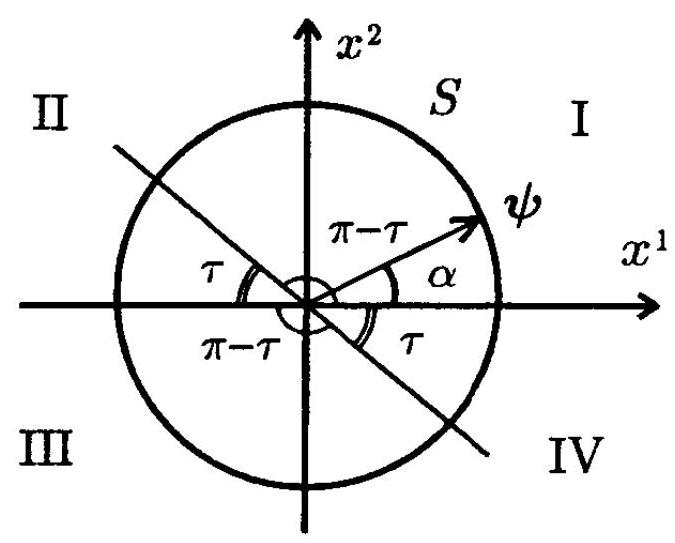
\includegraphics[max width=0.6\textwidth]{images/bo_d547okref24c73bgfch0_94_778_1455_675_543_0.jpg}
\end{center}
\hspace*{3em} 

Рис. 29

Таким образом, в зависимости от того, в какой сектор по- падает вектор ψ, заданный формулами (7.12), получаем разные выражения для опорной функции. Учитывая формулы (7.12) и тот факт, что \(\parallel \mathbf{\psi }\parallel  = 1\) , окончательно имеем выражение

\[
c\left( {X\left( t\right) ,\psi }\right)  = \left\{  \begin{array}{cc} \left( {1 - \cos \tau }\right) {\psi }^{1} + \sin \tau  \cdot  {\psi }^{2}, & \psi  \in  \mathrm{I}, \\  2\parallel \psi \parallel  + \left( {1 + \cos \tau }\right) {\psi }^{1} - \sin \tau  \cdot  {\psi }^{2}, & \psi  \in  \mathrm{{II}}, \\  \left( {-1 + \cos \tau }\right) {\psi }^{1} - \sin \tau  \cdot  {\psi }^{2}, & \psi  \in  \mathrm{{III}}, \\  2\parallel \psi \parallel  - \left( {1 + \cos \tau }\right) {\psi }^{1} + \sin \tau  \cdot  {\psi }^{2}, & \psi  \in  \mathrm{{IV}}. \end{array}\right.
\]

(7.15)

Когда вектор и пробегает I и III секторы, то это — опорная функция одной точки

\[
\left( {1 - \cos \tau ,\sin \tau }\right) ,\;\left( {-1 + \cos \tau , - \sin \tau }\right) ,
\]

соответственно, а когда вектор ψ пробегает II и IV секторы, то это — опорная функция кругов

\[
{S}_{2}\left( {1 + \cos \tau , - \sin \tau }\right) ,\;{S}_{2}\left( {-1 - \cos \tau ,\sin \tau }\right) , \tag{7.16}
\]

соответственно. Множество достижимости \(X\left( t\right)\) , заданное опор- ной функцией (7.15), является пересечением двух кругов (7.16), оно изображено на рис. 30.

При \(\tau  = \pi\) опорная функция \(c\left( {X\left( {{t}_{0} + \pi }\right) ,\psi }\right)\) принимает по- стоянное значение 2 || ψ в секторах II и IV, сектора I и III вырождаются.Таким образом,имеем равенство

\[
X\left( {{t}_{0} + \pi }\right)  = {S}_{2}\left( 0\right)
\]

На рис. 31 показана динамика множеств достижимости X(t) при увеличении длины отрезка времени т = t – to в пределах от 0 до π.

Пример 3. Найти множество управляемости \(Y\left( t\right)\) на конеч- ное множество \({M}_{1} = \{ \mathbf{0}\}\) для управляемой системы

\[
\left\{  \begin{array}{l} {\dot{x}}^{1} = {x}^{2}, \\  {\dot{x}}^{2} = v,\;\left| v\right|  \leq  1. \end{array}\right.
\]

\begin{center}
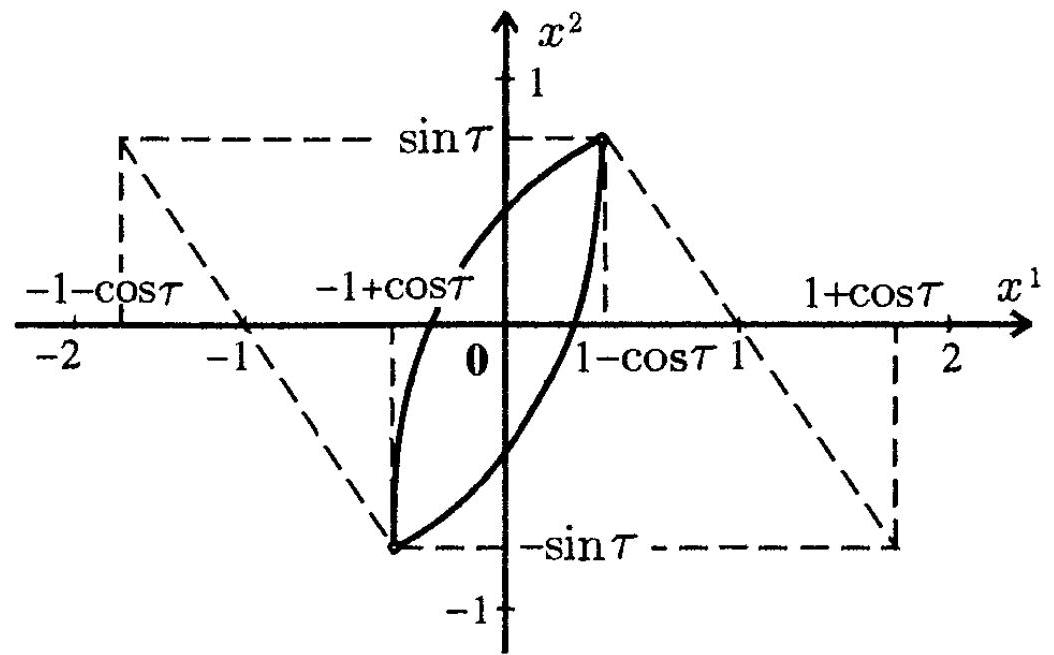
\includegraphics[max width=1.0\textwidth]{images/bo_d547okref24c73bgfch0_96_201_0_1054_655_0.jpg}
\end{center}
\hspace*{3em} 

Pac. 30

\begin{center}
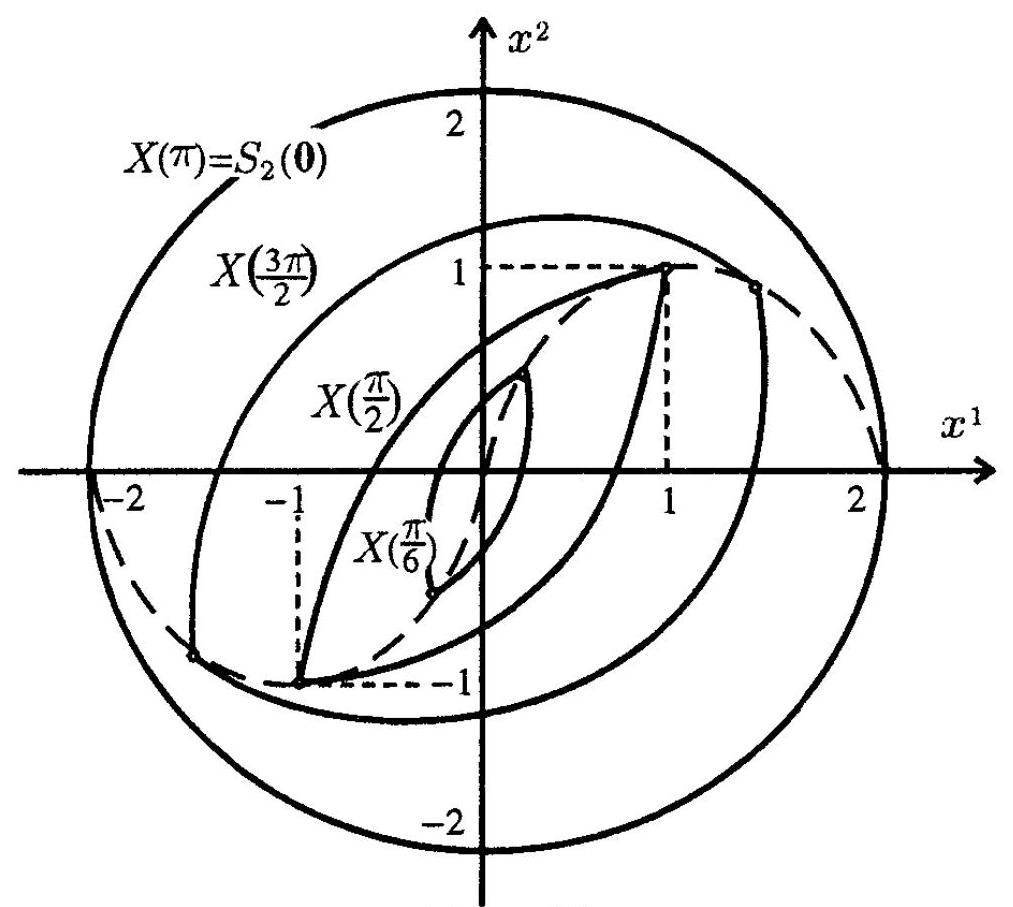
\includegraphics[max width=0.9\textwidth]{images/bo_d547okref24c73bgfch0_96_221_774_1013_907_0.jpg}
\end{center}
\hspace*{3em} 

Рис. 31

Вновь перейдем к стандартному виду (7.1), положив и = \(= \left( {{u}^{1},{u}^{2}}\right)  = \left( {0,v}\right)\) . Таким образом, множество

\[
U = \left\{  {u \in  {E}^{2} : {u}^{1} = 0,\left| {u}^{2}\right|  \leq  1}\right\}
\]

является отрезком в фазовом пространстве E2, ero опорная функция имеет вид

\[
\mathrm{c}\left( {U,\psi }\right)  = \left| {\psi }^{2}\right|
\]

Экспоненциал матрицы \(A = \left( \begin{array}{ll} 0 & 1 \\  0 & 0 \end{array}\right)\) был вычислен в приме- pe 3 (см. лекцию 6). Он имеет вид

\[
{e}^{tA} = \left( \begin{array}{ll} 1 & t \\  0 & 1 \end{array}\right)
\]

Подставляя все эти данные в формулу (7.10), получаем для опорной функции множества управляемости \(Y\left( t\right)\) следующее вы- ражение в зависимости от длины отрезка \(\tau  = {t}_{1} - t\) :

\[
\mathrm{c}\left( {Y\left( t\right) ,\psi }\right)  = {\int }_{0}^{\tau }\left| {{\psi }^{1}s - {\psi }^{2}}\right| {ds}. \tag{7.17}
\]

Под знаком интеграла в формуле (7.17) стоит модуль ли- нейной функции. Вычисление этого интеграла распадается на четыре случая.

1. Если при всех 0 ≤ \(s \leq  \tau\) выполняется неравенство Ф1* 5 – \(- {\psi }^{2} \geq  0\) , то, очевидно, получаем выражение

\[
c\left( {Y\left( t\right) ,\psi }\right)  = \frac{1}{2}{\tau }^{2}{\psi }^{1} - \tau {\psi }^{2}. \tag{7.18}
\]

2. Если при всех 0 ≤ \(s \leq  \tau\) выполняется неравенство Ф1* 5 – \(- {\psi }^{2} \leq  0\) ,то получаем выражение

\[
\mathrm{c}\left( {Y\left( t\right) ,\psi }\right)  =  - \frac{1}{2}{\tau }^{2}{\psi }^{1} + \tau {\psi }^{2}. \tag{7.19}
\]

3. Пусть существует \(0 < {s}^{ * } < \tau\) такое, что \({\psi }^{1}{s}^{ * } - {\psi }^{2} = 0\), и пусть \({\psi }^{1} > 0\). Тогда подынтегральная функция имеет график, изображенный на рис. 32, и интеграл в формуле (7.17) можно вычислить отдельно на отрезках \([0,s^{ * }]\) и \(\left[ {s}^{ * },\tau \right]\). Таким образом, получаем выражение

\[
c\left( {Y\left( t\right) ,\psi }\right)  = \frac{{\left( {\psi }^{2}\right) }^{2}}{{\psi }^{1}} + \frac{1}{2}{\tau }^{2}{\psi }^{1} - \tau {\psi }^{2}. \tag{7.20}
\]

4. Аналогично для случая \({\psi }^{1} < 0\) имеем

\[
c\left( {Y\left( t\right) ,\psi }\right)  =  - \frac{{\left( {\psi }^{2}\right) }^{2}}{{\psi }^{1}} - \frac{1}{2}{\tau }^{2}{\psi }^{1} + \tau {\psi }^{2}. \tag{7.21}
\]

\begin{center}
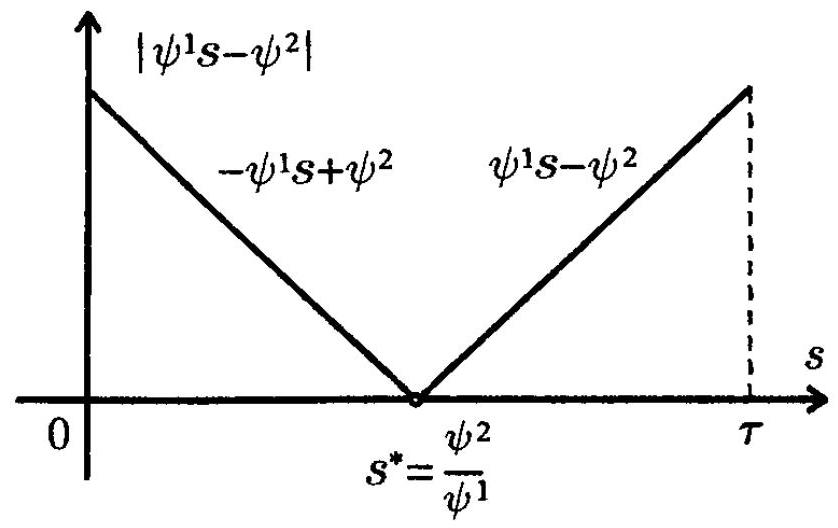
\includegraphics[max width=0.8\textwidth]{images/bo_d547okref24c73bgfch0_98_310_0_838_528_0.jpg}
\end{center}
\hspace*{3em} 

Рис. 32

Нетрудно убедиться, что выпуклое компактное множество \(Y\left( t\right)\) , изображенное на рис. 33, имеет опорную функцию, которая задается формулами (7.18)-(7.21). Это множество \(Y\left( t\right)\) ограни- чено двумя параболами

\[
{x}^{1} = \frac{1}{2}{\tau }^{2} - \frac{1}{2}{\left( {x}^{2} + \tau \right) }^{2},\;{x}^{1} =  - \frac{1}{2}{\tau }^{2} + \frac{1}{2}{\left( {x}^{2} - \tau \right) }^{2}.
\]

Читателям предлагается проверить это самостоятельно.

На рис. 34 показана динамика множества управляемости \(Y\left( t\right)\) при увеличении длины отрезка времени т \(= {t}_{1} - t\) .

\begin{center}
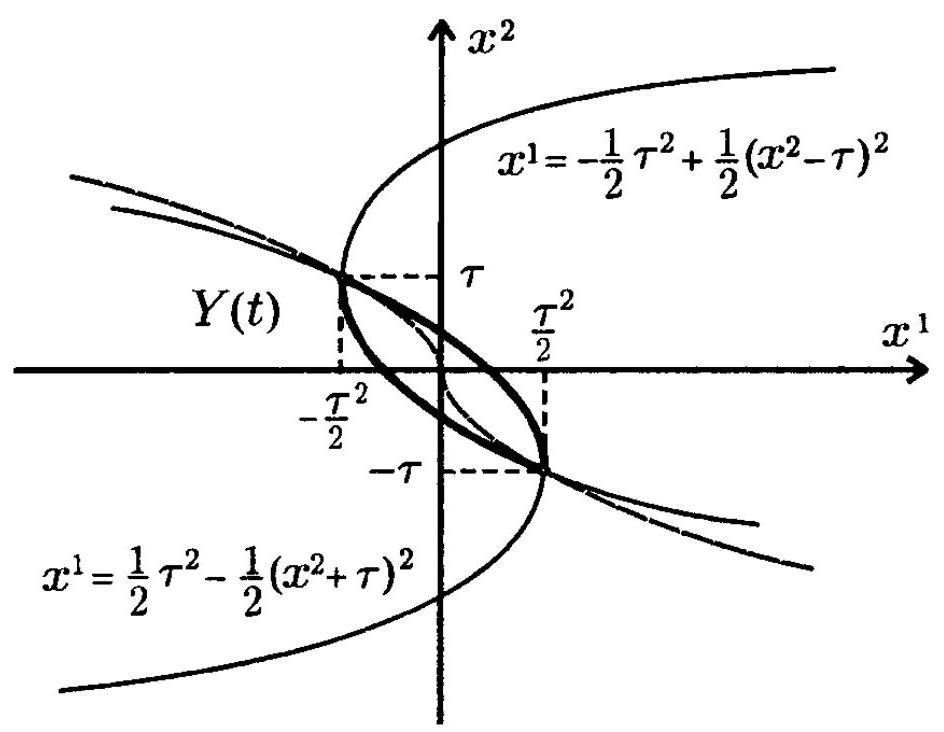
\includegraphics[max width=0.9\textwidth]{images/bo_d547okref24c73bgfch0_98_260_1304_944_732_0.jpg}
\end{center}
\hspace*{3em} 

Рис. 33

\begin{center}
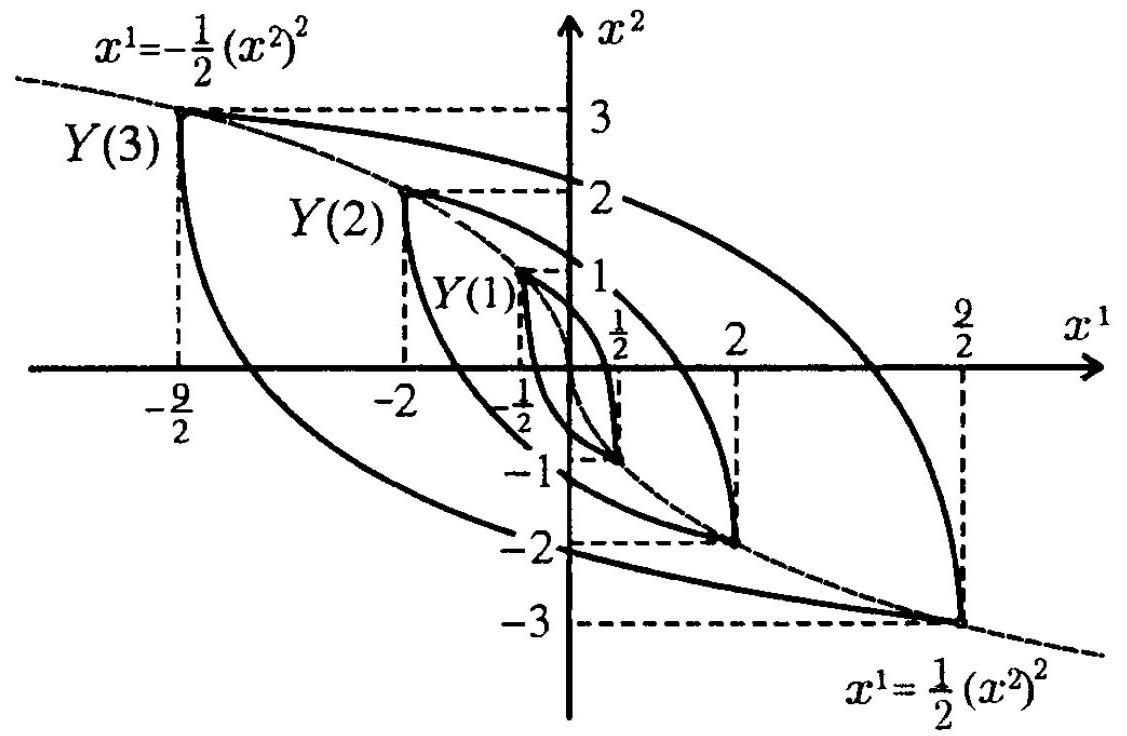
\includegraphics[max width=1.0\textwidth]{images/bo_d547okref24c73bgfch0_99_164_0_1127_736_0.jpg}
\end{center}
\hspace*{3em} 

Рис. 34

\section*{7.3. Задачи}

1. Найдите для управляемой системы

\[
\left\{  \begin{array}{l} {\dot{x}}^{1} = {x}^{2}, \\  {\dot{x}}^{2} =  - {x}^{1} + v,\;\left| v\right|  \leq  1 \end{array}\right. \tag{7.22}
\]

множество достижимости \(X\left( t\right)\) при \(t \geq  \pi\) из начального множес- тва \({M}_{0} = \{ 0\}\) .

2. Найдите для управляемой системы (7.22) множество управляемости \(Y\left( t\right)\) для конечного множества \({M}_{1} = \{ \mathbf{0}\}\) .

3. Найдите для управляемой системы

\[
\left\{  \begin{array}{l} {\dot{x}}^{1} = {x}^{2}, \\  {\dot{x}}^{2} = v,\;0 \leq  v \leq  1 \end{array}\right. \tag{7.23}
\]

множество достижимости X(t) из начального множества \({M}_{0} = \{ \mathbf{0}\}\) .

4. Найдите для управляемой системы (7.23) множество до- стижимости \(X\left( t\right)\) из начального множества

\[
{M}_{0} = \left\{  {\mathbf{x}}_{0}\right\}   = \{ \left( {0,1}\right) \} .
\]

5. Найдите для управляемой системы (7.23) множество управляемости \(Y\left( t\right)\) для конечного множества \({M}_{1} = \{ \mathbf{0}\}\) .

6. Haßдите для управляемой системы

\[
\left\{  \begin{array}{l} {\dot{x}}^{1} = {x}^{2} + {u}^{1}, \\  {\dot{x}}^{2} =  - {x}^{1} + {u}^{2},\;u \in  {S}_{1}\left( 0\right)  \end{array}\right.
\]

множество достижимости X(t) из начального множества

\[
{M}_{0} = \left\{  {\mathbf{x} \in  {E}^{2} : \left| {x}^{1}\right|  \leq  2,{x}^{2} = 0}\right\}  .
\]

7. Найдите для управляемой системы

\[
\left\{  \begin{array}{l} {\dot{x}}^{1} = {x}^{2} + {u}^{1}, \\  {\dot{x}}^{2} =  - {x}^{1} + {u}^{2},\;u \in  \{  - v,v\}  \end{array}\right.
\]

где v ∈ \({E}^{2} -\) некоторый фиксированный вектор, множество управляемости \(Y\left( t\right)\) для \(t = \pi\) на конечное множество

\[
{M}_{1} = \left\{  {\mathbf{x} \in  {E}^{2} : {x}^{1} = 0,\left| {x}^{2}\right|  \leq  1}\right\}  .
\]

8. Докажите, что если М0 = \{0\} и множество U симметрич- ное, т.е. для любого \(u \in  U\) справедливо включение — \(u \in  U\) , то для любой управляемой системы (7.1) множество достижимости \(X\left( t\right)\) всегда будет симметричным.

9. Докажите, что для случая \({M}_{0} = \left\{  {\mathbf{x}}_{0}\right\}\) опорная функция множества достижимости \(c\left( {X\left( t\right) ,\mathbf{\psi }}\right)\) всегда непрерывно диффе- ренцируема по времени и для любого фиксированного вектора \(\psi  \in  {E}^{n}\) .

10. Докажите, что если бы не цен и о е и, то множество достижимости \(X\left( t\right)\) pacширяется со временем \(t\) ,т.е. при \({t}^{\prime } < {t}^{\prime \prime }\) справедливо включение \(X\left( {t}^{\prime }\right)  \subset  X\left( {t}^{\prime \prime }\right)\) .

11. Докажите, что если \({M}_{1} = \{ 0\}\) и \(0 \in  U\) , то множество управляемости сужается со временем t, т.е. при б’ < t’ справед- ливо включение \(Y\left( {t}^{\prime }\right)  \supset  Y\left( {t}^{\prime \prime }\right)\) .

\section*{JIEKIUN 8}

\begin{itemize}\relax
\item\relax Задача управляемости.
\end{itemize}

\begin{itemize}\relax
\item\relax Теорема об управляемости.
\end{itemize}

\begin{itemize}\relax
\item\relax Лемма о внутренней точке интеграла.
\end{itemize}

\begin{itemize}\relax
\item\relax Локальная управляемость линейных систем.
\end{itemize}

\begin{itemize}\relax
\item\relax Постаточные условия локальной управляемости.
\end{itemize}

\section*{8.1. Общая задача управляемости}

Рассмотрим управляемый объект, описываемый уравнением

\[
\dot{\mathbf{x}} = A\mathbf{x} + \mathbf{u}, \tag{8.1}
\]

где, как обычно, \(\mathbf{x} \in  {E}^{n}\) - вектор фазового состояния объекта, \(\mathbf{u} \in  {E}^{n}\) - вектор управления, \(A\) — квадратная матрица разме- ром n x n. Допустимым управлением является произвольная из- меримая функция \(\mathbf{u}\left( t\right)  \in  U,U \in  \Omega \left( {E}^{n}\right)\) . Пусть заданы начальное и конечное множества \({M}_{0},{M}_{1} \in  \Omega \left( {E}^{n}\right)\) . Задача управляемости заключается в установлении следующего факта: существует ли на некотором отрезке времени [t, t, q) хотя бы одно такое допустимое управление и(t), что соответствующее ему решение \(\mathbf{x}\left( t\right)\) ypaвнения (8.1) удовлетворяет граничным условиям

\[
\mathbf{x}\left( {t}_{0}\right)  \in  {M}_{0},\;\mathbf{x}\left( {t}_{1}\right)  \in  {M}_{1}. \tag{8.2}
\]

Заметим, что в задаче управляемости мы не оцениваем качество перехода из множества \({M}_{0}\) на \({M}_{1}\) .

Будем говорить, что объект является управляемым на отрез- ке времени \(I = \left\lbrack  {{t}_{0},{t}_{1}}\right\rbrack\) из множества \({M}_{0}\) на множество \({M}_{1}\) , если существует хотя бы одно допустимое управление \(\mathbf{u}\left( t\right)\) такое, что соответствующее ему решение \(\mathbf{x}\left( t\right)\) удовлетворяет гранич- ным условиям (8.2), т.е. осуществляет переход из начального множества \({M}_{0}\) на конечное множество \({M}_{1}\) на отрезке времени \(\left\lbrack  {{t}_{0},{t}_{1}}\right\rbrack\) .

Определим функцию \(\varphi  : {E}^{n} \rightarrow  {E}^{1}\) соотношением

\[
\varphi \left( \psi \right)  = c\left( {{M}_{0},{e}^{\left( {{t}_{1} - {t}_{0}}\right) {A}^{ * }}\psi }\right)  + c\left( {{M}_{1}, - \psi }\right)  + {\int }_{0}^{{t}_{1} - {t}_{0}}c\left( {U,{e}^{s{A}^{ * }}\psi }\right) {ds}.
\]

(8.3)

Теорема об управляемости. Пусть множества \({M}_{0}\) и \({M}_{1}\) выпуклы. Тогда объект является управляемым на отрез- ке времени \(\left\lbrack  {{t}_{0},{t}_{1}}\right\rbrack\) из множества \({M}_{0}\) на множество \({M}_{1}\) тогда и только тогда, когда для любого вектора \(\psi  \in  S\) функция управляемости неотрицательна, т.е.

\[
\varphi \left( \psi \right)  \geq  0, \tag{8.4}
\]

а это в свою очередь эквивалентно условию

\[
{\varphi }_{0} = \mathop{\min }\limits_{{\psi  \in  S}}\varphi \left( \psi \right)  \geq  0 \tag{8.5}
\]

Доказательство. Очевидно, что объект является управ- ляемым на отрезке времени \(\left\lbrack  {{t}_{0},{t}_{1}}\right\rbrack\) из множества \({M}_{0}\) на множест- во \({M}_{1}\) тогда и только тогда, когда для множества достижимости \(X\left( {t}_{1}\right)\) выполнено соотношение

\[
X\left( {t}_{1}\right)  \cap  {M}_{1} \neq  \varnothing \tag{8.6}
\]

Так как множество \({M}_{1}\) выпукло и согласно свойству 3 множеств достижимости (см. лекцию 7) множество \(X\left( {t}_{1}\right)\) также выпукло, то в силу следствия из свойства 12 опорных функций (см. лек- цию 3) выполнение соотношения (8.6) эквивалентно выполне- нию неравенства

\[
c\left( {X\left( {t}_{1}\right) ,\psi }\right)  + c\left( {{M}_{1}, - \psi }\right)  \geq  0
\]

для любого вектора \(\psi  \in  S\) . Подставляя в это выражение опор- ную функцию множества достижимости \(X\left( {t}_{1}\right)\) при \(\tau  = {t}_{1} - {t}_{0}\) (см. формулу (7.6) из лекции 7), мы получаем эквивалентное выражение

\[
c\left( {{M}_{0},{e}^{\left( {{t}_{1} - {t}_{0}}\right) {A}^{ * }}\psi }\right)  + \mathop{\int }\limits_{0}^{{{t}_{1} - {t}_{0}}}c\left( {U,{e}^{s{A}^{ * }}\psi }\right) {ds} + c\left( {{M}_{1}, - \psi }\right)  \geq  0.
\]

которое также должно выполняться для любого вектора \(\psi  \in  {E}^{n}\) . Но в силу положительной однородности опорных функций (свой- ство 1 из лекции 3) это соотношение достаточно проверить лишь для векторов \(\psi  \in  S\) , а это эквивалентно выполнению неравенства (8.4). Функция управляемости \(\varphi \left( \psi \right)\) непрерывна, так как все опорные функции в формуле (8.3) непрерывны по следствию свойства 13 (см. лекцию 3), а множество \(S \subset  {E}^{n}\) компактно. Таким образом, условие (8.4) эквивалентно усло- вию (8.5). Теорема доказана.

Заметим, что при доказательстве теоремы об управляемости вместо соотношения (8.6) можно было бы использовать соотно- шение

\[
{M}_{0} \cap  Y\left( {t}_{0}\right)  \neq  \varnothing
\]

где \(Y\left( t\right)\) — множество управляемости, и получить неравенство, эквивалентное неравенству (8.4).

Если множества \({M}_{0},{M}_{1} \in  \Omega \left( {E}^{n}\right)\) не являются выпуклыми, то мы не получим полного критерия управляемости. Только в одну сторону из управляемости объекта (8.1) на отрезке вре- мени [1, 0, 1] будет следовать, что функция управляемости φ(ф) удовлетворяет неравенству (8.4).

Отметим также, что функция управляемости \(\varphi \left( \psi \right)\) зависит лишь от длины отрезка времени т = to -1. Таким образом, для любого отрезка времени [t, t,1] длины т она принимает одина- ковые значения.

Теорема об управляемости позволяет находить или оцени- вать такой отрезок времени \(I = \left\lbrack  {{t}_{0},{t}_{1}}\right\rbrack\) ,на котором объект яв- ляется управляемым. Проиллюстрируем это на примерах.

Пример 1. Пусть уравнение (8.1) имеет вид

\[
\left\{  \begin{array}{l} {\dot{x}}^{1} =  - {x}^{2}, \\  {\dot{x}}^{2} = {x}^{1} + v,\;\left| v\right|  \leq  1, \end{array}\right. \tag{8.7}
\]

а множества \({M}_{0}\) и \({M}_{1}\) заданы условиями

\[
{M}_{0} = \left\{  {\mathbf{x} \in  {E}^{2} : {x}^{1} =  - 5,\left| {x}^{2}\right|  \leq  1}\right\}  ,\;{M}_{1} = \{ 0\} .
\]

Опорные функции множеств М0, М1 и И в данном случае имеют вид

\[
c\left( {{M}_{0},\psi }\right)  =  - 5{\psi }^{1} + \left| {\psi }^{2}\right| ,\;c\left( {{M}_{1},\psi }\right)  = 0,\;c\left( {U,\psi }\right)  = \left| {\psi }^{2}\right| .
\]

Экспоненциал матрицы A* = ( \(\left( \begin{array}{rr} 0 & 1 \\   - 1 & 0 \end{array}\right)\) yxe подсчитан (см. пример 2 из лекции 6) и имеет вид

\[
{e}^{t{A}^{ * }} = \left( \begin{array}{rr} \cos t & \sin t \\   - \sin t & \cos t \end{array}\right) .
\]

Произвольный вектор \(\psi  \in  S \subset  {E}^{2}\) зададим в виде \(\psi  = \; = \left( {\cos \alpha ,\sin \alpha }\right)\) . В результате из формулы (8.3) получим, что неравенство (8.4) выполняется тогда и только тогда, когда для любого параметра \(0 \leq  \alpha  \leq  {2\pi }\) при \(\tau  = {t}_{1} - {t}_{0}\) выполняется неравенство

\[
\varphi \left( \psi \right)  = \varphi \left( \alpha \right)  =
\]

\[
=  - 5\cos \left( {\alpha  - \tau }\right)  + \left| {\sin \left( {\alpha  - \tau }\right) }\right|  + {\int }_{0}\left| {\sin \left( {\alpha  - s}\right) }\right| {ds} \geq  0.
\]

Ясно, что если \(\tau  = {t}_{1} - {t}_{0} \geq  {3\pi }\) , то это неравенство заведомо выполняется для любого \(0 \leq  \alpha  \leq  {2\pi }\) .

Таким образом, если отрезок времени [и, и] имеет длину т, то объект, описываемый уравнением (8.7), заведомо является управляемым на этом отрезке.

Пример 2. Рассмотрим управляемую систему

\[
\left\{  \begin{array}{l} {\dot{x}}^{1} = {x}^{2} + {u}^{1}, \\  {\dot{x}}^{2} =  - {x}^{1} + {u}^{2},\;u \in  {S}_{1}\left( 0\right) , \end{array}\right. \tag{8.8}
\]

c множеством начальных состояний \({M}_{0} = {S}_{\pi }\left( \left( {{3\pi },0}\right) \right)\) и мно- жеством конечных состояний \({M}_{1} = {S}_{\pi }\left( 0\right)\) (puc. 35). Tpeбуется определить отрезок времени [и, и, на котором система явля- ется управляемой из множества М0 на множество М1. Пусть \(\tau  = {t}_{1} - {t}_{0}.\)

Экспоненцалматрицы \(A = \left( \begin{array}{rr} 0 & 1 \\   - 1 & 0 \end{array}\right)\) имеетвид

\[
{e}^{t{A}^{ * }} = \left( \begin{array}{rr} \cos t & \sin t \\   - \sin t & \cos t \end{array}\right) ,
\]

аопорные \(\phi\) ункциимножеств \(U,{M}_{0},{M}_{1}\) задаются выражениями

\[
c\left( {U,\psi }\right)  = \parallel \psi \parallel ,\;c\left( {{M}_{0},\psi }\right)  = {3\pi }{\psi }^{1} + \pi \parallel \psi \parallel ,\;c\left( {{M}_{1},\psi }\right)  = \pi \parallel \psi \parallel .
\]

Подставляя эти данные в формулу (8.3), получим функцию

\[
\varphi \left( \psi \right)  = {3\pi }\left( {{\psi }^{1}\cos \tau  - {\psi }^{2}\sin \tau }\right)  + {2\pi }\parallel \psi \parallel  + \tau \parallel \psi \parallel .
\]

\begin{center}
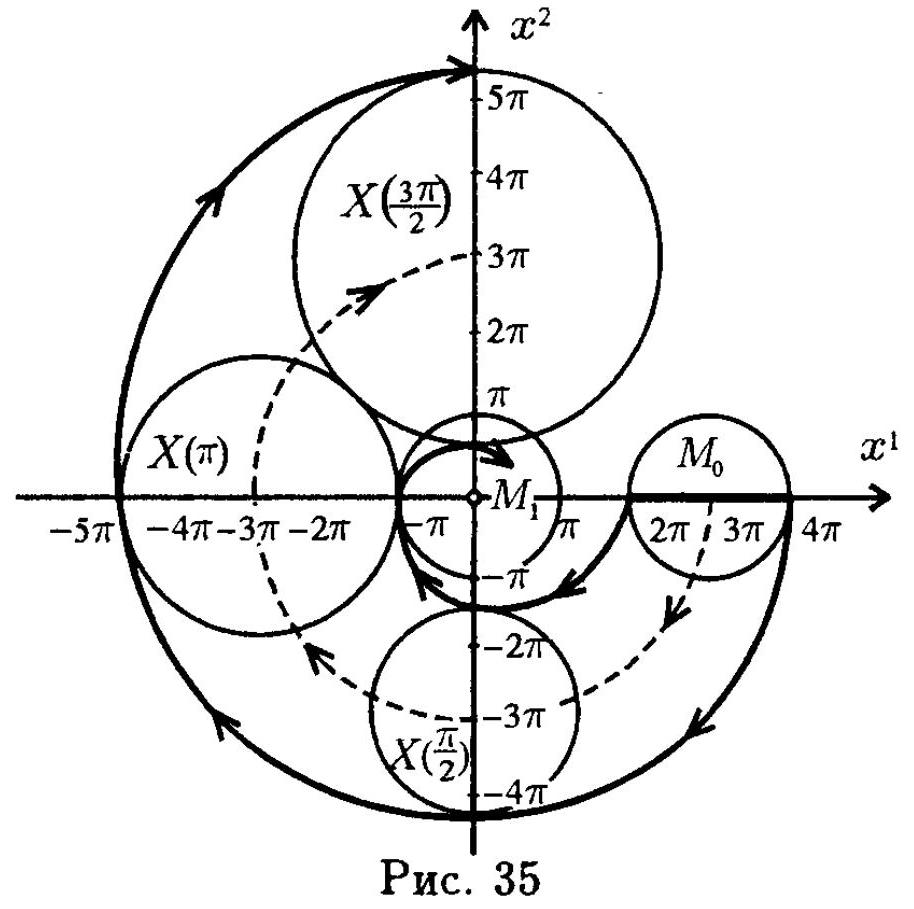
\includegraphics[max width=0.8\textwidth]{images/bo_d547okref24c73bgfch0_105_275_0_914_909_0.jpg}
\end{center}
\hspace*{3em} 

управляемости в следующем виде:

Таким образом, справедливо соотношение

\[
{\varphi }_{0} = \mathop{\min }\limits_{{\psi  \in  S}}\varphi \left( \psi \right)  = \tau  - \pi
\]

Следовательно, система (8.8) является управляемой из \({M}_{0}\) в \({M}_{1}\) на любом отрезке времени [и, б, 1, длина которого 7 больше или равна \(\pi\) , \(u\) не является управляемой ни на каком отрезке времени \(\left\lbrack  {{t}_{0},{t}_{1}}\right\rbrack\) ,длина которого меньше \(\pi\) .

Проиллюстрируем эти выкладки геометрически. Построим для этого множество достижимости Х(н). Для этого, подста- вив полученные данные в формулу (7.6) из лекции 7, получим следующее выражение для опорной функции множества дости- жимости в зависимости от длины отрезка времени т \(= t - {t}_{0}\) :

\[
c\left( {X\left( t\right) ,\psi }\right)  = {3\pi }\cos \tau  \cdot  {\psi }^{1} - {3\pi }\sin \tau  \cdot  {\psi }^{2} + \left( {\pi  + \tau }\right) \parallel \psi \parallel .
\]

Таким образом, множество достижимости X(t) есть круг ради- yca \(r\left( \tau \right)  = \pi  + \tau\) c центром в точке a( \(\tau\) ) = (3 π cos \(\tau\) , -3 π sin \(\tau\) ). Это множество изображено на рис. 35. Из рисунка видно, что при \(\tau  < \pi\) множества \(X\left( t\right)\) и \({M}_{1}\) не пересекаются,при \(\tau  = \pi\) происходит их первое касание и при т с я эти множества всегда пересекаются.

\section*{8.2. Лемма о внутренней точке интеграла}

Итак, для решения общей задачи управляемости получены необходимые и достаточные условия. Рассмотрим один част- ный, но часто встречающийся на практике случай управляе- мости, а именно, локальную управляемость. Для ее изучения потребуется следующая лемма.

Лемма о внутренней точке интеграла. Пусть заданы \(A - \kappa\) вадратная матрица размером \(n \times  n\) , \(v - {npou}\) звольный вектор из пространства E" и число τ > 0. Тогда

\[
0 \in  \operatorname{int}{\int }_{0}^{\tau }{e}^{sA}\{  - v,v\} {ds} \tag{8.9}
\]

тогда и только тогда, когда векторы v, Av, ... , лич и линей- но независимы.

Здесь под знаком интеграла в выражении (8.9) стоит мно- гозначное отображение \({e}^{sA}\) , которое получается для каждого \(0 \leq  s \leq  \tau\) как образ множества \{−v, v\}, coстоящего из двух точек, при линейном преобразовании евА.

Доказательство. Обозначим

\[
F = {\int }_{0}^{\tau }{e}^{sA}\{  - v,v\} {ds}
\]

Согласно теореме 1 (см. лекцию 5) множество F является не- пустым выпуклым и компактным подмножеством пространст- ва Е". Таким образом, в силу следствия из свойства 14 опорных функций (см. лекцию 3), точка х = 0 является внутренней для множества \(F\) тогда и только тогда, когда

\[
c\left( {F,\psi }\right)  > 0
\]

для любого вектора ф ∈ S.

Найдем опорную функцию множества F. Согласно теореме 2 (см. лекцию 5) и свойству 4 опорных функций имеем соотноше-

\[
c\left( {F,\psi }\right)  = c\left( {{\int }_{0}^{\tau }{e}^{sA}\{  - \mathbf{v},\mathbf{v}\} {ds},\psi }\right)  = {\int }_{0}^{\tau }c\left( {{e}^{sA}\{  - \mathbf{v},\mathbf{v}\} ,\psi }\right) {ds} =
\]

\[
= {\int }_{0}^{\tau }c\left( {\{  - \mathbf{v},\mathbf{v}\} ,{e}^{s{A}^{ * }}\psi }\right) {ds}.
\]

Опорная функция множества \(\{  - v,v\}\) известна,она имеет вид

\[
c\left( {\{  - \mathbf{v},\mathbf{v}\} ,\mathbf{\psi }}\right)  = \left| {\langle \mathbf{v},\mathbf{\psi }\rangle }\right| .
\]

Таким образом,получаем равенство

\[
c\left( {F,\psi }\right)  = {\int }_{0}^{\tau }\left| \left\langle  {v,{e}^{s{A}^{ * }}\psi }\right\rangle  \right| {ds} = {\int }_{0}^{\tau }\left| \left\langle  {{e}^{sA}v,\psi }\right\rangle  \right| {ds}.
\]

Следовательно, \(\mathbf{0} \in  \operatorname{int}F\) тогдаитолько тогда,когда

\[
{\int }_{0}^{\tau }\left| \left\langle  {{e}^{sA}v,\psi }\right\rangle  \right| {ds} > 0
\]

для любого вектора ф ∈ S. Поскольку подынтегральная функ- ция в последнем неравенстве непрерывна и неотрицательна, это неравенство эквивалентно выполнению условия

\[
\left\langle  {{e}^{tA}v,\psi }\right\rangle   \neq  0 \tag{8.10}
\]

на отрезке \(\left\lbrack  {0,\tau }\right\rbrack\) для любого вектора ф ∈ S. Покажем, что для этого необходимо и достаточно, чтобы векторы v, \(A\mathbf{v},\ldots ,{A}^{n - 1}\mathbf{v}\) были линейно независимы.

Докажем необходимость. Предположим противное, т.е. пусть условие (8.10) выполнено, а векторы v, \(A\mathbf{v},\ldots ,{A}^{n - 1}\mathbf{v}\) линейно зависимы. Тогда существует вектор \(\psi  \in  S\) такой,что

\[
\langle \mathbf{v},\mathbf{\psi }\rangle  = \langle A\mathbf{v},\mathbf{\psi }\rangle  = \ldots  = \left\langle  {{A}^{n - 1}\mathbf{v},\mathbf{\psi }}\right\rangle   = 0. \tag{8.11}
\]

Из курса алгебры (теорема Гамильтона — Келли) известно, что для матрицы \(A\) размером \(n \times  n\) все матрицы \({A}^{p}\) при \(p \geq  n\) являются линейными комбинациями матриц E, A, . . ., A \({}^{n - 1}\) . По определению экспоненциала еча (см. лекцию 6) имеем равенство

\[
{e}^{tA} = E + {tA} + \ldots  + \frac{{t}^{n - 1}}{\left( {n - 1}\right) !}{A}^{n - 1} + \frac{{t}^{n}}{n!}{A}^{n} + \ldots  =
\]

\[
= {c}_{1}\left( t\right) E + {c}_{2}\left( t\right) A + \ldots  + {c}_{n}\left( t\right) {A}^{n - 1}.
\]

В силу соотношений (8.11) отсюда получаем, что

\[
\left\langle  {{e}^{tA}v,\psi }\right\rangle   = {c}_{1}\left( t\right) \langle v,\psi \rangle  + {c}_{2}\left( t\right) \langle {Av},\psi \rangle  + \ldots  + {c}_{n}\left( t\right) \left\langle  {{A}^{n - 1}v,\psi }\right\rangle   \equiv  0,
\]

а это противоречит условию (8.10).

Достаточность также докажем от противного. Пусть векто- ры v, \({Av},\ldots ,{A}^{n - 1}v\) линейно независимы,но существует вектор \(\psi  \in  S\) raκoй,что

\[
\left\langle  {{e}^{tA}v,\psi }\right\rangle   \equiv  0
\]

на отрезке [0, 7]. Поскольку \(\tau  > 0\) , продифференцируем полу- ченное тождество \(n - 1\) pa3 по t и положим во всех производных \(t = 0\) . Тогда, oчевидно,имеем

\[
\langle \mathbf{v},\mathbf{\psi }\rangle  = \langle A\mathbf{v},\mathbf{\psi }\rangle  = \ldots  = \left\langle  {{A}^{n - 1}\mathbf{v},\mathbf{\psi }}\right\rangle   = 0.
\]

Tak как вектор \(\psi  \neq  0\) , orсюда следует,что векторы \(v,{Av},\ldots\) ..., \({A}^{n - 1}v\) линейно зависимы. Полученное противоречие завер- maer доказательство леммы.

\section*{8.3. Локальная управляемость}

Предположим, что конечное множество \({M}_{1} \in  \Omega \left( {E}^{n}\right)\) зада- но, a начальное множество \({M}_{0} = \left\{  {\mathbf{x}}_{0}\right\}\) ,где хо — произвольная точка из некоторой окрестности множества М1. Исследуем воз- можность перехода из некоторой окрестности \({S}_{\varepsilon }\left( {M}_{1}\right)\) на мно- жество \({M}_{1}\) для объекта, описываемого уравнением (8.1), при всевозможных допустимых управлениях и(t).

Управляемый объект, описываемый уравнением (8.1), назы- вается локально управляемым на множество \({M}_{1}\) на отрезке времени \(\left\lbrack  {{t}_{0},{t}_{1}}\right\rbrack\) , если существует \(\varepsilon  > 0\) такое, что для любой точки \({\mathbf{x}}_{0} \in  {M}_{1} + {S}_{\varepsilon }\left( \mathbf{0}\right)\) объект является управляемым на отрезке \(\left\lbrack  {{t}_{0},{t}_{1}}\right\rbrack\) из начального множества \({M}_{0} = \left\{  {\mathbf{x}}_{0}\right\}\) на конечное множес- тво \({M}_{1}\) . Это означает, что для любой точки \({\mathbf{x}}_{0} \in  {M}_{1} + {S}_{\varepsilon }\left( \mathbf{0}\right)\) существует допустимое управление \(\mathbf{u}\left( t\right)\) такое, что соответствующее решение \(\mathbf{x}\left( t\right)\) уравнения (8.1) перейдет из точки \({\mathbf{x}}_{0}\) в некото- рую точку множества \({M}_{1}\) на отрезке времени \(\left\lbrack  {{t}_{0},{t}_{1}}\right\rbrack\) (рис. 36).

\begin{center}
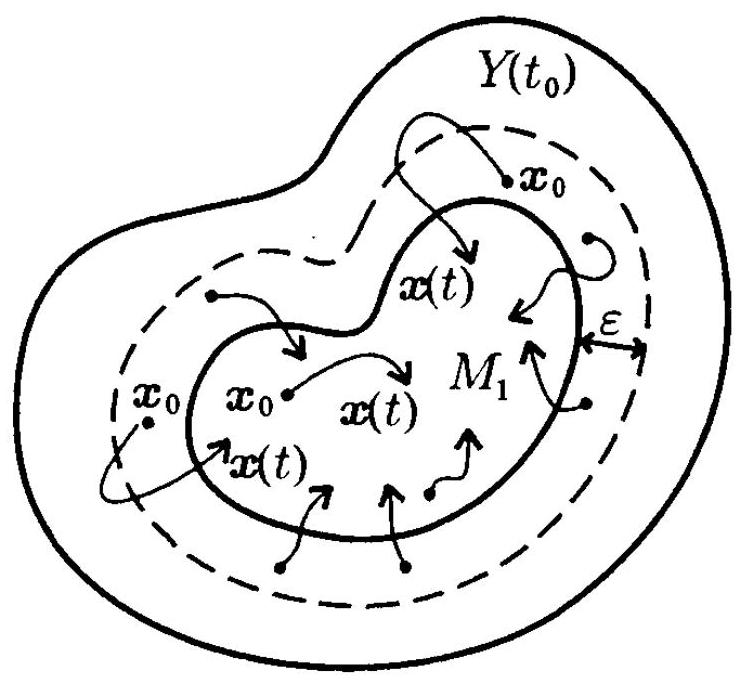
\includegraphics[max width=0.7\textwidth]{images/bo_d547okref24c73bgfch0_109_26_5_739_681_0.jpg}
\end{center}
\hspace*{3em} 

Рис. 36

Замечание. Данное определение локальной уп- равляемости на множество \({M}_{1}\) эквивалентно тому,что

\[
{M}_{1} \subset  \operatorname{int}Y\left( {t}_{0}\right) \tag{8.12}
\]

где \(Y\left( {t}_{0}\right)  -\) множество управляемости. Действительно, если объект локально управля- ем на множество \({M}_{1}\) , то существует ε > 0 такое, что любая точка \({\mathbf{x}}_{0} \in  {M}_{1} + Y\left( {t}_{0}\right)\) принадлежит множеству управляемости \(Y\left( {t}_{0}\right)\) ,следовательно, справедливо включение

\[
{M}_{1} + {S}_{\varepsilon }\left( 0\right)  \subset  Y\left( {t}_{0}\right) \tag{8.13}
\]

и, следовательно, включение (8.12). В другую сторону, если вы- полняется включение (8.12), то для любой точки m ∈ M1 cy- ществует число бет) > 0 такое, что справедливо соотношение \({\widetilde{S}}_{\varepsilon \left( m\right) }\left( \mathbf{m}\right)  \subset  Y\left( {t}_{0}\right)\) . Здесь \({\widetilde{S}}_{\varepsilon \left( m\right) }\left( \mathbf{m}\right)\) - открытый шар радиуса \(\varepsilon \left( \mathbf{m}\right)\) c центром в точке m. Совокупность всех шаров \({\widetilde{S}}_{\varepsilon \left( \mathbf{m}\right) }\left( \mathbf{m}\right)\) при \(\mathbf{m} \in  {M}_{1}\) образует открытое покрытие компактного множес- тва М1. По соответствующей теореме из курса математического анализа из этого покрытия можно выбрать конечное подпокры- тие \({\widetilde{S}}_{\varepsilon \left( {m}_{1}\right) }\left( {\mathbf{m}}_{1}\right) ,\ldots ,{\widetilde{S}}_{\varepsilon \left( {m}_{r}\right) }\left( {\mathbf{m}}_{r}\right)\) . Выбирая \(\varepsilon  = \mathop{\min }\limits_{{1 \leq  i \leq  r}}\varepsilon \left( {\mathbf{m}}_{i}\right)\) , получаем включение (8.13), эквивалентное локальной управля- емости объекта (8.1) на множество \({M}_{1}\) .

В уравнении (8.1) можно сделать замену переменных х на \(\mathbf{x} - {\mathbf{x}}_{1}\) . Уравнение объекта опять будет иметь вид (8.1), только множество \(U\) сдвигается на постоянный вектор \(A{\mathbf{x}}_{1}\) . Поэтому достаточно рассмотреть лишь один случай локальной управля- емости при \({x}_{1} = 0\) .

Итак, наш объект является локально управляемым в точке \(\mathbf{x} = \mathbf{0}\) на отрезке времени \(I = \left\lbrack  {{t}_{0},{t}_{1}}\right\rbrack\) , если существует число \(\varepsilon  > 0\) такое, что для любой точки \({\mathbf{x}}_{0} \in  {S}_{\varepsilon }\left( \mathbf{0}\right)\) объект является управляемым на отрезке времени \(\left\lbrack  {{t}_{0},{t}_{1}}\right\rbrack\) из начального множес- тва \({M}_{0} = \left\{  {\mathbf{x}}_{0}\right\}\) на конечное множество \({M}_{1} = \{ \mathbf{0}\}\) .

Для решения общей задачи управляемости мы доказали тео- рему об управляемости. Применяя эту теорему и лемму о внут- ренней точке интеграла, получим достаточное условие локаль- ной управляемости в точке х = 0.

Теорема о локальной управляемости. Пусть сущест- вует вектор \(\mathbf{v} \in  {E}^{n}\) такой, что выполнены следующие два условия:

1) векторы — v и v принадлежат множеству U;

2) векторы \(\mathbf{v},A\mathbf{v},\ldots ,{A}^{n - 1}\mathbf{v}\) линейно независимы.

Тогда объект является локально управляемым в точке \(\mathbf{x} = \mathbf{0}\) на любом отрезке времени \(I = \left\lbrack  {{t}_{0},{t}_{1}}\right\rbrack  ,\tau  = {t}_{1} - {t}_{0} > 0\) .

Доказательство. По теореме об управляемости объект является локально управляемым в точке \(\mathbf{x} = \mathbf{0}\) на отрезке вре- мени \(I = \left\lbrack  {{t}_{0},{t}_{1}}\right\rbrack\) , если существует \(\varepsilon  > 0\) такое, что для любого \({\mathbf{x}}_{0} \in  {S}_{\varepsilon }\left( \mathbf{0}\right)\) и любого \(\mathbf{\psi } \in  S\) выполняется условие

\[
c\left( {\left\{  {\mathbf{x}}_{0}\right\}  ,{e}^{t{A}^{ * }}\mathbf{\psi }}\right)  + c\left( {\{ \mathbf{0}\} , - \mathbf{\psi }}\right)  + {\int }_{0}^{\tau }c\left( {U,{e}^{s{A}^{ * }}\mathbf{\psi }}\right) {ds} \geq  0.
\]

Вычисляя опорные функции множеств \{x0\} и \{0\}, преобразуем это неравенство в следующее:

\[
{\int }_{0}^{\tau }c\left( {U,{e}^{s{A}^{ * }}\psi }\right) {ds} \geq   - \left\langle  {{\mathbf{x}}_{0},{e}^{\tau {A}^{ * }}\psi }\right\rangle  . \tag{8.14}
\]

Покажем существование \(\varepsilon  > 0\) такого, что неравенство (8.14) выполняется для любого \({\mathbf{x}}_{0} \in  {S}_{\varepsilon }\left( 0\right)\) и любого \(\mathbf{\psi } \in  S\) . Для этого покажем,что левая часть неравенства (8.14),не зависящая от ε, для любого вектора ф ∈ S больше или равна некоторого числа \(\alpha  > 0\) , a правая часть неравенства (8.14) выбором числа \(\varepsilon  > 0\) может быть сделана сколь угодно малой.

По предположению 1) теоремы выполняется включение \(\{  - \mathbf{v},\mathbf{v}\}  \in  U\) . Согласно свойству 6 опорных функций (см. лек- цию 3) для любого вектора цб с S получаем неравенство

\[
\left\{  {-{\sigma }_{1}{\sigma }^{2}}\right\}   \subset  {U}^{c\left( {\{  - v,v\} ,\psi }\right)  \leq  c\left( {U\left( v\right) ,\psi }\right) .}
\]

\[
{\int }_{0}^{\tau }c\left( {U,{e}^{s{A}^{ * }}\psi }\right) {ds} \geq  {\int }_{0}^{\tau }c\left( {\{  - v,v\} ,{e}^{s{A}^{ * }}\psi }\right) {ds} =
\]

\[
= c\left( {{\int }_{0}^{\tau }{e}^{sA}\{  - v,v\} {ds},\psi }\right) . \tag{8.15}
\]

По предположению 2) теоремы векторы v, Av, …, A \({}^{n - 1}\) v линей- но независимы. По лемме о внутренней точке интеграла это означает, что

\[
\mathbf{0} \in  \operatorname{int}{\int }_{0}^{\tau }{e}^{sA}\{  - v,v\} {ds}
\]

Таким образом, в силу свойства 14 опорных функций (см. лек- цию 3) имеем строгое неравенство

\[
c\left( {{\int }_{0}^{\tau }{e}^{sA}\{  - \mathbf{v},\mathbf{v}\} {ds},\psi }\right)  > 0
\]

для любого вектора ψ ∈ S. Но опорная функция непрерывна по вектору \(\psi\) , a единичная сфера S — компактное множество в пространстве \({E}^{n}\) , поэтому существует число α > 0 такое, что

\[
c\left( {{\int }_{{t}_{0}}^{{t}_{1}}{e}^{-{sA}}\{  - \mathbf{v},\mathbf{v}\} {ds},\psi }\right)  \geq  \alpha  > 0
\]

для всех векторов \(\psi  \in  S\) . Согласно соотношению (8.15) для любого вектора ф \(\in  S\) имеем оценку

\[
{\int }_{0}^{\tau }c\left( {U,{e}^{s{A}^{ * }}\psi }\right) {ds} \geq  \alpha  > 0 \tag{8.16}
\]

Рассмотрим теперь правую часть неравенства (8.14). Так как \({\mathbf{x}}_{0} \in  {S}_{\varepsilon }\left( \mathbf{0}\right)\) , то для любого вектора ф ∈ S справедливо соотношение

\[
\left\langle  {{\mathbf{x}}_{0},\mathbf{\psi }}\right\rangle   \leq  c\left( {{S}_{\varepsilon }\left( \mathbf{0}\right) ,\mathbf{\psi }}\right)  = \varepsilon \parallel \mathbf{\psi }\parallel .
\]

114

\[
\left| {\langle {x}_{0},\varphi \rangle }\right|  \leq  \parallel x \land  \varphi \parallel  \leq  \varepsilon \;\text{ below }
\]

\[
\text{ here is Koevan - Synovics }
\]

Таким образом, получаем оценки

\[
- \left\langle  {{\mathbf{x}}_{0},{e}^{\tau {A}^{ * }}\mathbf{\psi }}\right\rangle   = \left\langle  {{\mathbf{x}}_{0}, - {e}^{\tau {A}^{ * }}\mathbf{\psi }}\right\rangle   \leq  \varepsilon \left\lVert \begin{array}{c} {-{e}^{\tau {A}^{ * }}\mathbf{\psi }} \end{array} \right\rVert \leq  \varepsilon \left\lVert \begin{array}{c} {e}^{\tau {A}^{ * }} \end{array} \right\rVert \cdot  \parallel \mathbf{\psi }\parallel .
\]

(8.17)

Следовательно, если выбрать число б ≤ ( \(\frac{\alpha }{\left\lVert \begin{array}{c} {e}^{\tau {A}^{ * }} \end{array} \right\rVert}\) , то для любого вектора \(\psi  \in  S\) получим неравенство

\[
- \left\langle  {{\mathbf{x}}_{0},{e}^{\tau {A}^{ * }}\psi }\right\rangle   \leq  \alpha
\]

Сравнивая полученное неравенство с условием (8.16), заклю- чаем, что существует \(\varepsilon  > 0\) такое, что соотношение (8.14) вы- полняется для любого вектора фе S. А это означает, что объ- ект является локально управляемым в точке х = 0 на отрезке времени \(\left\lbrack  {{t}_{0},{t}_{1}}\right\rbrack\) . Теорема доказана.

Теорема о локальной управляемости позволяет для мно- гих объектов довольно просто доказывать локальную управля- emocть.

Пример 3. Докажем, что объект, описываемый системой уравнений

\[
\left\{  \begin{array}{l} {\dot{x}}^{1} = {x}^{2}, \\  {\dot{x}}^{2} =  - {x}^{1} + {u}^{2},\;\left| {u}^{2}\right|  \leq  1, \end{array}\right.
\]

является локально управляемым в точке х = 0 на любом отрезке времени \(\left\lbrack  {{t}_{0},{t}_{1}}\right\rbrack  ,{t}_{0} \neq  {t}_{1}\) . Покажем, что для такого объекта вы- полняются предположения теоремы о локальной управляемости. Действительно, если v = (0,1), то векторы - v, v принадлежат множеству \(U = \left\{  {u \in  {E}^{2} : {u}^{1} = 0,\left| {u}^{2}\right|  \leq  1}\right\}\) , т.е. первое пред- положение выполнено. Проверим, что векторы v, \(A\mathbf{v}\) линейно независимы. Лействительно, векторы

\[
\mathbf{v} = \left( \begin{array}{l} 0 \\  1 \end{array}\right) ,\;A\mathbf{v} = \left( \begin{array}{rr} 0 & 1 \\   - 1 & 0 \end{array}\right) \left( \begin{array}{l} 0 \\  1 \end{array}\right)  = \left( \begin{array}{l} 1 \\  0 \end{array}\right)
\]

линейно независимы. Итак, объект является локально управля- емым в точке х = 0.

Заметим, что теорема о локальной управляемости являет- ся лишь достаточным условием локальной управляемости, т.е. объект может быть локально управляемым, а предположения указанной теоремы при этом могут не выполняться. В этом случае для доказательства локальной управляемости нужно ис- пользовать общую теорему об управляемости. Проиллюстриру- ем это на примерах.

Пример 4. Рассмотрим объект, поведение которого описы- вается системой уравнений

\[
\left\{  \begin{array}{l} {\dot{x}}^{1} = {x}^{2}, \\  {\dot{x}}^{2} =  - {x}^{1} + {u}^{2},\;0 \leq  {u}^{2} \leq  1. \end{array}\right. \tag{8.18}
\]

Покажем, что этот объект является локально управляемым в точке \(\mathbf{x} = \mathbf{0}\) на отрезке времени \(I = \left\lbrack  {0,{2\pi }}\right\rbrack\) . Предположения теоремы о локальной управляемости для данного объекта не выполняются. Действительно, множество U имеет вид

\[
U = \left\{  {\mathbf{u} \in  {E}^{2} : {u}^{1} = 0,0 \leq  {u}^{2} \leq  1}\right\}  .
\]

Для этого множества единственный вектор \(v = 0\) удовлетворяет первому предположению теоремы, но этот вектор не удовлетво- ряет второму предположению теоремы.

Локальную управляемость докажем, используя общую тео- рему об управляемости. Покажем, что существует ε > 0 такое, что для любого \({\mathbf{x}}_{0} \in  {S}_{\varepsilon }\left( \mathbf{0}\right)\) объект является управляемым из множества \({M}_{0} = \left\{  {\mathbf{x}}_{0}\right\}\) на множество \({M}_{1} = \{ \mathbf{0}\}\) на отрезке вре- мени \(I = \left\lbrack  {0,{2\pi }}\right\rbrack\) . Для этого достаточно проверить неравенство (8.4) для любого вектора ψ ∈ S. Экспоненциал ейК* в данном случае имеет вид

\[
{e}^{t{A}^{ * }} = \left( \begin{array}{rr} \cos t & \sin t \\   - \sin t & \cos t \end{array}\right) .
\]

Опорные функции множеств \({M}_{0},{M}_{1},U\) задаются соотноше- ниями

\[
c\left( {{M}_{0},\psi }\right)  = \left\langle  {{\mathbf{x}}_{0},\psi }\right\rangle  ,\;c\left( {{M}_{1},\psi }\right)  = 0,\;c\left( {U,\psi }\right)  = \frac{1}{2}{\psi }^{2} + \frac{1}{2}\left| {\psi }^{2}\right| .
\]

Записав произвольный вектор \(\psi  \in  S \subset  {E}^{2}\) в виде \(\psi  = (\cos \alpha\) , sin \(\alpha\) ) и подставив в формулу (8.3), получим следующее выра- жение для функции управляемости:

\[
\varphi \left( \mathbf{\psi }\right)  = \varphi \left( \alpha \right)  = \left\langle  {{\mathbf{x}}_{0},\left( \begin{array}{c} \cos \alpha \\  \sin \alpha \end{array}\right) }\right\rangle   +
\]

\[
+ {\int }_{0}^{2\pi }\left\lbrack  {\frac{1}{2}\sin \left( {\alpha  + s}\right)  + \frac{1}{2}\left| {\sin \left( {\alpha  + s}\right) }\right| }\right\rbrack  {ds}.
\]

Интеграл в этом выражении равен 2 при всех 0 ≤ \(\alpha  \leq  {2\pi }\) , следовательно,

\[
{\varphi }_{0} = \mathop{\min }\limits_{{\psi  \in  S}}\varphi \left( \psi \right)  =  - \left\lVert \begin{array}{c} {\mathbf{x}}_{0} \end{array} \right\rVert + 2.
\]

Итак, можно выбрать \(\varepsilon  = 2\) , и при этом из любой точки \({\mathbf{x}}_{0} \in  {S}_{2}\left( \mathbf{0}\right)\) на отрезке времени [0,2π] можно перейти в точку \(\mathbf{x} = \mathbf{0}\) по решению уравнения (8.18) при допустимом управлении \(\mathbf{u}\left( t\right)\) . Таким образом, объект является локально управляемым в точке \(x = 0\) на отрезке времени [0,2 \(\pi\) ].

Отметим, что в примере 4 локальная управляемость имеет место не на любом отрезке времени \(\left\lbrack  {{t}_{0},{t}_{1}}\right\rbrack\) . Если длину этого отрезка уменьшать, то в какой-то момент локальная управляе- мость исчезнет.

Пример 5. Пусть 0 ∈ int U. Покажем, что такой объект всегда является управляемым в точке х = 0 для любой матрицы \(A\) paзмером \(n \times  n\) на любом ненулевом отрезке времени [ \({t}_{0},{t}_{1}\) ].

Теорема о локальной управляемости здесь не всегда при- менима, например, для матрицы \(A = 0\) ее предположения не выполнены. Воспользуемся общей теоремой об управляемости.

Согласно предположению, существует число δ > 0 такое, что \({S}_{\delta }\left( \mathbf{0}\right)  \subset  U\) , следовательно, справедливо неравенство

\[
c\left( {U,\psi }\right)  \geq  c\left( {{S}_{\delta }\left( \mathbf{0}\right) ,\psi }\right)  = \delta \parallel \psi \parallel .
\]

Подставляязто неравенство и выражения

\[
c\left( {{M}_{0},\mathbf{\psi }}\right)  = \left\langle  {{\mathbf{x}}_{0},\mathbf{\psi }}\right\rangle  ,\;c\left( {{M}_{1},\mathbf{\psi }}\right)  = 0
\]

в формулу (8.3), для функции управляемости

\[
\varphi \left( \mathbf{\psi }\right)  = \left\langle  {{\mathbf{x}}_{0},{e}^{\tau {A}^{ * }}\mathbf{\psi }}\right\rangle   + {\int }_{0}^{\tau }c\left( {U,{e}^{s{A}^{ * }}\mathbf{\psi }}\right) {ds}
\]

сучетом формулы (8.17) получим следующее неравенство:

\[
\varphi \left( \mathbf{\psi }\right)  \geq   - \varepsilon \left\lVert \begin{array}{c} {e}^{\tau {A}^{ * }} \end{array} \right\rVert \cdot  \parallel \mathbf{\psi }\parallel  + \delta {\int }_{0}^{\tau }\left\lVert \begin{array}{c} {{e}^{s{A}^{ * }}\mathbf{\psi }} \end{array} \right\rVert{ds}.
\]

В силу непрерывности при всех \(\psi  \in  S\) справедливо неравенство

\[
{\int }_{0}^{\tau }\left\lVert \begin{array}{c} {{e}^{s{A}^{ * }}\psi } \end{array} \right\rVert{ds} \geq  \alpha  > 0
\]

Таким образом, если выбрать

\[
0 < \varepsilon  \leq  \frac{\delta \alpha }{\left\lVert \begin{array}{c} {e}^{\tau {A}^{ * }} \end{array} \right\rVert}
\]

то при всех ход E \({S}_{\varepsilon }\left( 0\right)\) и всех у е д получим неравенство \(\varphi \left( \mathbf{\psi }\right)  \geq  0\) . Следовательно, объект является локально управля- емым.

Если нужно исследовать локальную управляемость точки \(\mathbf{x} \neq  \mathbf{0}\) , то, делая замену переменных \(\mathbf{x}\) на \(\mathbf{x} - {\mathbf{x}}_{1}\) в уравнении (8.1), получаем новый управляемый объект

\[
\dot{\mathbf{x}} = A\mathbf{x} + \mathbf{u},\;\mathbf{u} \in  {U}^{\prime } = U + A{\mathbf{x}}_{1}. \tag{8.19}
\]

Его управляемость в точке х = 0 эквивалентна управляемости уравнения (8.1) в точке х = х .

Пример 6. Рассмотрим управляемую систему

\[
\left\{  \begin{array}{l} {\dot{x}}^{1} = {x}^{2} \\  {\dot{x}}^{2} = {u}^{2} \end{array}\right. \tag{8.20}
\]

Покажем, что на любом ненулевом отрезке времени эта система является локально управляемой в любой точке прямой из е 10 на плоскости \({E}^{2}\) .

Возьмем произвольную точку хочу = ( \({x}^{1},0\) ) этой прямой и вычислим множество \({U}^{\prime }\) . Поскольку

\[
A{\mathbf{x}}_{0} = \left( \begin{array}{ll} 0 & 1 \\  0 & 0 \end{array}\right) \left( \begin{array}{l} {\mathbf{x}}^{1} \\  0 \end{array}\right)  = \left( \begin{array}{l} 0 \\  0 \end{array}\right) ,
\]

множества U’ и U совпадают. Таким образом, локальная управ- ляемость в любой точке \({\mathbf{x}}_{0} = \left( {{\mathbf{x}}^{1},0}\right)\) имеет место, ecли доказана управляемость системы (8.20) в точке 0.

Выберем вектор \(v = \left( {0,1}\right)\) . Для него выполняются оба пред- положения теоремы о локальной управляемости. Действитель- но, оба вектора ±v принадлежат множеству U = \(\left\{  {u \in  {E}^{2} : {u}^{1} = }\right. \; = 0,\left| {u}^{2}\right|  \leq  1\}\) , a beкторы

\[
\mathbf{v} = \left( \begin{array}{l} 0 \\  1 \end{array}\right) \;\mathbf{u}\;A\mathbf{v} = \left( \begin{array}{ll} 0 & 1 \\  0 & 0 \end{array}\right) \left( \begin{array}{l} 0 \\  1 \end{array}\right)  = \left( \begin{array}{l} 1 \\  0 \end{array}\right)
\]

линейно независимы. Таким образом, объект (8.20) является ло- кально управляемым в любой точке (х, 0) ∈ E’.

Замечание. Рассмотрим произвольное множество \({M}_{1} \in \; \in  \Omega \left( {E}^{n}\right)\) . Если для каждой его точки \({\mathbf{x}}_{1} \in  {M}_{1}\) объект, onисывае- мый уравнением (8.1), является локально управляемым в точку \(\mathbf{x} = {\mathbf{x}}_{1}\) на отрезке времени [ \({t}_{0},{t}_{1}\) ], то он будет также локально управляемым на этом же отрезке времени [t, t] на все конеч- ное множество \({M}_{1}\) . Действительно, в силу локальной управля- емости в произвольной точке \({\mathbf{x}}_{1} \in  {M}_{1}\) выполняется включение \({\mathbf{x}}_{1} \in  \operatorname{int}Y\left( {t}_{0}\right)\) , a оно эквивалентно локальной управляемости на множество \({M}_{1}\) в силу его компактности (см. замечание в начале данного раздела).

Пример 7. Покажем, что управляемая система

\[
\dot{\mathbf{x}} = \mathbf{u},\;\mathbf{u} \in  {S}_{1}\left( 0\right)
\]

локально управляема на любое конечное множество \({M}_{1} \in  \Omega \left( {E}^{n}\right)\) на любом отрезке времени \(\left\lbrack  {{t}_{0},{t}_{1}}\right\rbrack\) .

Возьмем произвольную точку х, н с ли. В данном примере \(A = 0\) , поэтому и’ \(U = U\) (см. формулу (8.19)) и из локальной управляемости в точке х = 0 следует его локальная управля- емость в любой точке \({\mathbf{x}}_{1} \in  {M}_{1}\) . В силу данного выше замеча- ния теперь объект является локально управляемым на множес- тво \({M}_{1}\) .

\section*{8.4. Задачи}

1. Найдите отрезок времени [t, t, h] на котором объект, опи- сываемый системой уравнений

\[
\left\{  \begin{array}{l} {\dot{x}}^{1} = {x}^{2} + {u}^{1}, \\  {\dot{x}}^{2} =  - {x}^{1} + {u}^{2},\;u \in  {S}_{1}\left( 0\right) , \end{array}\right.
\]

является управляемым из начального множества \({M}_{0} = \{ 0\}\) на конечное множество \({M}_{1} = \left\{  {x \in  {E}^{2} : {x}^{1} = 0,{10} \leq  {x}^{2} \leq  {12}}\right\}\) .

2. Является ли объект, описываемый системой уравнений

\[
\left\{  \begin{array}{l} {\dot{x}}^{1} = {u}^{1}, \\  {\dot{x}}^{2} =  - {x}^{2} + {u}^{2},\;\left| {u}^{1}\right|  \leq  1,\left| {u}^{2}\right|  \leq  1, \end{array}\right.
\]

управляемым из начального множества \({M}_{0} = \{ \left( {-3,4}\right) \}\) на ко- нечное множество \({M}_{1} = \{ 0\}\) на отрезке времени \(\left\lbrack  {0,3}\right\rbrack\) ?

3.Квляется ли объект, описываемый системой уравнений

\[
\left\{  \begin{array}{l} {\dot{x}}^{1} = {x}^{2} + {u}^{1}, \\  {\dot{x}}^{2} =  - {x}^{1} + {u}^{2},\;u \in  {S}_{1}\left( 0\right)  \subset  {E}^{3}, \\  {\dot{x}}^{3} = {u}^{3}, \end{array}\right.
\]

управляемым из начального множества \({M}_{0} = {S}_{1}\left( \mathbf{0}\right)  \subset  {E}^{3}\) на конечное множество \({M}_{1} = \{ \left( {4,2,2}\right) \}\) на отрезке времени [0,4 \(\pi\) ]?

4. Является ли объект, описываемый системой уравнений

\[
\left\{  \begin{array}{l} {\dot{x}}^{1} =  - {x}^{1} - \pi {x}^{2} + {u}^{1}, \\  {\dot{x}}^{2} = \pi {x}^{1} - {x}^{2} + {u}^{2},\;u \in  {S}_{1}\left( 0\right)  \subset  {E}^{2}, \end{array}\right.
\]

управляемым из начального множества

\[
{M}_{0} = \left\{  {\mathbf{x} \in  {E}^{2} : \left| {{x}^{1} - 8}\right|  \leq  1,\left| {x}^{2}\right|  \leq  1}\right\}
\]

на конечное множество

\[
{M}_{1} = \left\{  {\mathbf{x} \in  {E}^{2} : \left| {x}^{1}\right|  + \left| {{x}^{2} - 1}\right|  \leq  1}\right\}
\]

на отрезке времени [—1,1]?

5. Докажите, что объект, описываемый системой уравнений

\[
\left\{  \begin{array}{l} {\dot{x}}^{1} = {x}^{2} \\  {\dot{x}}^{2} = {u}^{2},\;\left| {u}^{2}\right|  \leq  1 \end{array}\right.
\]

является локально управляемым на конечное множество \({M}_{1} = \; = {S}_{\frac{1}{2}}\left( 0\right)\) на любом ненулевом отрезке времени.

6. Докажите, что объект, описываемый системой уравнений

\[
\left\{  \begin{array}{l} {\dot{x}}^{1} = {x}^{2} + {u}^{1}, \\  {\dot{x}}^{2} =  - {x}^{1} + {u}^{2},\;u \in  {S}_{1}\left( \left( {1,0}\right) \right) , \end{array}\right.
\]

является локально управляемым в точке х = 0.

7. Докажите, что если 0 ∉ conv \(U\) , то объект, описываемый уравнением (8.1), не является локально управляемым, когда от- резок времени \(\left\lbrack  {{t}_{0},{t}_{1}}\right\rbrack\) достаточно мал.

\({\mathbf{8}}^{ * }\) . Пусть множество \(U\) выпукло и точка \(\mathbf{x} = \mathbf{0}\) лежит на границе \(U\) ,т.е. 0 ∈ \(\partial U\) . Рассмотрим множество

\[
K\left( U\right)  = \left\{  {\mathbf{x} \in  {E}^{n} : \mathbf{x} = \lambda \mathbf{u},\mathbf{u} \in  U,\lambda  \geq  0}\right\}  .
\]

Докажите, что если множество \(K\left( U\right)\) не содержит ни одной прямой из пространства E", то объект, описываемый уравнени- ем (8.1), не является локально управляемым на отрезке времени \(\left\lbrack  {{t}_{0},{t}_{1}}\right\rbrack\) достаточно малой длины.

9. Пусть 0 ∈ conv \(U\) и объект, описываемый уравнением (8.1), является управляемым из начального множества M0 = \{0\} на конечное множество \({M}_{1} \in  \Omega \left( {E}^{n}\right)\) на отрезке времени [0,7]. До- кажите, что этот объект будет управляемым на любом отрезке времени \(\left\lbrack  {0,{\tau }^{\prime }}\right\rbrack\) ,где \({\tau }^{\prime } > \tau\) .

10. Пусть объект, описываемый уравнением (8.1), является локально управляемым на конечное множество \({M}_{1}\) . Докажите, что для множества управляемости \(Y\left( t\right)\) при \({t}^{\prime } > t\) cnpaведливо BKЛЮЧение

\[
Y\left( t\right)  \subset  \operatorname{int}Y\left( {t}^{\prime }\right) \text{ . }
\]

11*. Пусть объект, описываемый уравнением (8.1), является локально управляемым в точке х = 0. Является ли он локально управляемым на конечное множество \({M}_{1} = {S}_{\varepsilon }\left( \mathbf{0}\right)\) при достаточ- но малых \(\varepsilon  > 0\) ?

\section*{ЛЕКЦИЯ 9}

\begin{itemize}\relax
\item\relax Теорема существования оптимального управления в линейной задаче быстродействия.
\end{itemize}

\begin{itemize}\relax
\item\relax Принцип максимума Понтрягина, его геометричес- кий смысл и эквивалентные формулировки.
\end{itemize}

\begin{itemize}\relax
\item\relax Теорема о необходимых условиях оптимальности.
\end{itemize}

\section*{9.1. Существование оптимального управления}

В предыдущей лекции был рассмотрен первый основной во- прос математической теории оптимального управления — во- прос об управляемости. Если задача управляемости решается положительно, т.е. существует хотя бы одно допустимое управ- ление, переводящее из начального множества Мо на конечное множество \({M}_{1}\) ,то можно перейти ко второму основному воп- росу — к вопросу существования оптимального управления.

Напомним постановку линейной задачи быстродействия. По- ведение объекта описывается уравнением

\[
\dot{\mathbf{x}} = A\mathbf{x} + \mathbf{u}, \tag{9.1}
\]

где х — л-мерный вектор фазового состояния объекта, и — \(n\) -мерный вектор управления, \(A\) - матрица размером \(n \times  n\) . Допустимым управлением и(t) называется произвольная изме- римая функция, удовлетворяющая включению и(t) ∈ U, где \(U \in  \Omega \left( {E}^{n}\right)\) . Начальный момент \({t}_{0}\) зафиксирован и заданы на- чальное и конечное множества \({M}_{0},{M}_{1} \in  \Omega \left( {E}^{n}\right)\) . Задача быстро- действия заключается в нахождении допустимого управления, переводящего объект из множества М0 на множество М1 за ми- нимальное время.

Теорема существования оптимального управления. Предположим, что объект является управляемым из мно- жества \({M}_{0}\) на множество \({M}_{1}\) на некотором отрезке време- ни \(\left\lbrack  {{t}_{0},{t}_{1}}\right\rbrack\) . Toгда существует оптимальное управление и*(t), \(t \in  \left\lbrack  {{t}_{0},{t}^{ * }}\right\rbrack\) , nepeводящее объект из множества МО на множес- тво М1 за минимальное время t* — tо.

Доказательство. Рассмотрим множество

\[
T = \left\{  {t \geq  {t}_{0} : X\left( t\right)  \cap  {M}_{1} \neq  \varnothing }\right\}  ,
\]

где \(X\left( t\right)\) — множество достижимости управляемой системы (9.1) на отрезке времени \(\left\lbrack  {{t}_{0},t}\right\rbrack\) из начального множества М0. По пред- положению теоремы множество T непусто. Обозначим через t* нижнюю грань моментов времени t ∈ \(T\) ,т.е.

\[
{t}^{ * } = \mathop{\inf }\limits_{{t \in  T}}t
\]

Нижняя грань \({t}^{ * }\) существует, поскольку множество T ограниче- но снизу моментом времени но. Таким образом, за время, строго меньшее чем \({t}^{ * } - {t}_{0}\) ,невозможно перейти из множества \({M}_{0}\) на множество \({M}_{1}\) c помощью какого-либо допустимого управления. Теперь нужно доказать, что существует допустимое управление \({\mathbf{u}}^{ * }\left( t\right)\) , nepeводящее объект из множества \({M}_{0}\) на множество \({M}_{1}\) ровно за время \({t}^{ * } - {t}_{0}\) ,т.е. на отрезке времени [ \({t}_{0},{t}^{ * }\) ], поскольку начальный момент времени и предполагается фиксированным.

Tak как \({t}^{ * }\) является нижней гранью моментов времени t ∈ \(T\) , то существует последовательность моментов н, сходящаяся к точке \({t}^{ * }\) , т.е. \({t}_{k} \rightarrow  {t}^{ * }\) при \(k \rightarrow  \infty\) , причем для каждого \({t}_{k}\) выпол- няется условие

\[
X\left( {t}_{k}\right)  \cap  {M}_{1} \neq  \varnothing
\]

Пусть для каждого \(k\) некоторая точка х, принадлежит этому пересечению, т.е.

\[
{x}_{k} \in  X\left( {t}_{k}\right)  \cap  {M}_{1}. \tag{9.2}
\]

Поскольку \({\mathbf{x}}_{k} \in  {M}_{1}\) , a множество \({M}_{1}\) — компакт,из последова- тельности \{x\} можно выбрать подпоследовательность, сходя- щуюся к некоторой точке

\[
{x}^{ * } \in  {M}_{1}\text{ . } \tag{9.3}
\]

Эту подпоследовательность снова обозначим через \{x\}.

Пусть задано произвольное число ε > 0. Так как последова- тельность \(\left\{  {\mathbf{x}}_{k}\right\}\) сходится к точке \({\mathbf{x}}^{ * }\) , то начиная с некоторого номера к1 будет выполняться условие \(\left\lVert \begin{array}{c} {{\mathbf{x}}^{ * } - {\mathbf{x}}_{k}} \end{array} \right\rVert \leq  \frac{\varepsilon }{2}\) . Таким образом, в силу формулы (9.2) имеем соотношение

\[
{\mathbf{x}}^{ * } = \left( {{\mathbf{x}}^{ * } - {\mathbf{x}}_{k}}\right)  + {\mathbf{x}}_{k} \in  {S}_{\frac{\varepsilon }{2}}\left( 0\right)  + X\left( {t}_{k}\right) . \tag{9.4}
\]

Множество достижимости \(X\left( t\right)\) непрерывно зависит от времени t (свойство 7 множеств достижимости из лекции 7). Поэтому, начиная с некоторого номера kg, будет выполняться включение

\[
X\left( {t}_{k}\right)  \subset  X\left( {t}^{ * }\right)  + {S}_{\frac{\varepsilon }{2}}\left( 0\right)
\]

(см. формулу (4.2) из лекции 4). Отсюда в силу соотношения (9.4) получаем включение

\[
{x}^{ * } \in  X\left( {t}^{ * }\right)  + {S}_{\varepsilon }\left( 0\right) .
\]

Таким образом, для любого числа ε > 0 справедливо представ- ление

\[
{\mathbf{x}}^{ * } = {\mathbf{x}}_{k} + {\mathbf{y}}_{k},\;{\mathbf{x}}_{k} \in  X\left( {t}^{ * }\right) ,\;{\mathbf{y}}_{k} \in  {S}_{\varepsilon }\left( 0\right) .
\]

Последовательность точек \{x\} сходится к точке x* при k → ∞, так как

\[
\left\lVert \begin{array}{c} {{\mathbf{x}}^{ * } - {\mathbf{x}}_{k}} \end{array} \right\rVert = \left\lVert \begin{array}{c} {\mathbf{y}}_{k} \end{array} \right\rVert \leq  \varepsilon  \rightarrow  0.
\]

Множество \(X\left( {t}^{ * }\right)\) компактно (свойство 2 множеств достижи- мости из лекции 7), следовательно, справедливо включение \({\mathbf{x}}^{ * } \in  X\left( {t}^{ * }\right)\) . Окончательно с учетом включения (9.3) получаем условие

\[
X\left( {t}^{ * }\right)  \cap  {M}_{1} \neq  \varnothing \text{ . }
\]

Это и означает по определению множества достижимости, что существует допустимое управление и «и), переводящее объект из множества \({M}_{0}\) на множество \({M}_{1}\) на отрезке времени \(\left\lbrack  {{t}_{0},{t}^{ * }}\right\rbrack\) . Теорема доказана.

Отметим здесь, что теорема существования оптимального управления доказана для любых непустых и компактных мно- жеств \(U,{M}_{0},{M}_{1}\) .

\section*{9.2. Принцип максимума Понтрягина}

Мы уже выяснили вопрос существования оптимального уп- равления в линейной задаче быстродействия. Теперь, если оп- тимальное управление существует, нужно научиться его нахо- дить. Для этого удобно использовать необходимые условия оп- тимальности. Это значит, что нужно найти такие условия, ко- торым заведомо удовлетворяет любое оптимальное управление, а затем искать оптимальное управление в множестве управле- ний, удовлетворяющих этим необходимым условиям.

Здесь можно привести аналогию с задачей поиска глобаль- ного минимума гладкой скалярной функции \(f\left( x\right)\) на числовой прямой \(x \in  {E}^{1}\) . Если гладкая функция \(f\left( x\right)\) достигает минимума в точке \({x}^{ * }\) , то выполняется условие \({f}^{\prime }\left( {x}^{ * }\right)  = 0\) . Таким образом, coothollehme

\[
{f}^{\prime }\left( x\right)  = 0 \tag{9.5}
\]

является необходимым условием минимума. Этому соотноше- нию, кроме точки глобального минимума х*, удовлетворяют все точки локального минимума, все точки максимума, а также все точки перегиба, в которых касательная к графику функции \(f\left( x\right)\) горизонтальна. Однако в конкретных практических задачах со- отношению (9.5), как правило, удовлетворяет конечное число точек, а из них даже простым перебором можно найти точку глобального минимума.

В рассматриваемой линейной задаче быстродействия также нужно найти минимум скалярной функции, т.е. время перехода \({t}_{1} - {t}_{0}\) объекта из множества \({M}_{0}\) на множество \({M}_{1}\) ,только ар- гументами этой функции являются не скалярные величины, а всевозможные допустимые управления \(\mathbf{u}\left( t\right)  \in  U\) . Тем не менее в линейной задаче быстродействия можно получить очень эф- фективные необходимые условия оптимальности. Таким необхо- димым условием оптимальности является принцип максимума Понтрягина. Дадим его формулировку.

Принцип максимума Понтрягина. Пусть на отрезке времени \(I = \left[ t_{0},t_{1}\right]\) задано некоторое допустимое управление \(\mathbf{u}\left( t\right)\) такое, что соответствующее решение \(\mathbf{x}(t)\) уравнения (9.1) переводит объект из начального множества \(M_{0}\) на конечное множество \(M_{1}\) на отрезке времени \(I = \left[ t_{0},t_{1}\right]\), т.е. удовлетворяет граничным условиям \(\mathbf{x}\left( t_{0}\right) \in M_{0}\), \(\mathbf{x}\left( t_{1}\right) \in M_{1}\). Будем говорить, что пара \(\mathbf{u}\left( t\right), \mathbf{x}\left( t\right)\) удовлетворяет принципу максимума Понтрягина на отрезке времени \(I = \left[ t_{0},t_{1}\right]\), если существует такое нетривиальное решение \(\psi(t)\) вспомогательной системы дифференциальных уравнений

\[
\dot{\psi } =  - {A}^{ * }\psi , \tag{9.6}
\]

что выполнены следующие три условия:

\[
\langle \mathbf{u}\left( t\right) ,\mathbf{\psi }\left( t\right) \rangle  = c\left( {U,\mathbf{\psi }\left( t\right) }\right) \tag{9.7}
\]

для почти всех t ∈ I;

2) условие трансверсальности на множестве М0

\[
\left\langle  {\mathbf{x}\left( {t}_{0}\right) ,\mathbf{\psi }\left( {t}_{0}\right) }\right\rangle   = c\left( {{M}_{0},\mathbf{\psi }\left( {t}_{0}\right) }\right) ; \tag{9.8}
\]

3) условие трансверсальности на множестве М1

\[
\left\langle  {\mathbf{x}\left( {t}_{1}\right) , - \psi \left( {t}_{1}\right) }\right\rangle   = c\left( {{M}_{1}, - \psi \left( {t}_{1}\right) }\right) . \tag{9.9}
\]

Система дифференциальных уравнений (9.6) называется сопряженной, а ее решение \(\psi(t)\) -- сопряженной функцией. Это решение \(\psi(t)\) называется нетривиальным, если \(\psi(t) \not\equiv 0\).

В силу теоремы 1 (см. лекцию 6) решение \(\psi(t)\) сопряженной линейной системы уравнений (9.6) существует на всем отрезке времени \(I = \left[ t_{0},t_{1}\right]\), единственно для любого начального значения \(\psi \left( t_{0}\right)\) и задается формулой Коши

\[
\psi \left( t\right)  = {e}^{\left( {{t}_{0} - t}\right) {A}^{ * }}\psi \left( {t}_{0}\right) . \tag{9.10}
\]

Это решение ψ(t) нетривиально, если ψ(t) ≠ 0, поскольку мат- рица \({e}^{\left( {{t}_{0} - t}\right) {A}^{ * }}\) невырождена. Если начальное значение для сопря- женной функции \(\psi \left( t\right)\) задано на правом конце отрезка \(\left\lbrack  {{t}_{0},{t}_{1}}\right\rbrack\) ,т.е. в точке \({t}_{1}\) , то решение фи() системы уравнений (9.6) имеет вид (см. формулу (6.9) из лекции 6)

\[
\psi \left( t\right)  = {e}^{\left( {{t}_{1} - t}\right) {A}^{ * }}\psi \left( {t}_{1}\right) . \tag{9.11}
\]

Это решение будет нетривиальным, если ψ(+) ≠ 0, также в силу невырожденности экспоненциала е (и-é) А*.

Пусть сопряженная функция \(\mathbf{\psi }\left( t\right)\) задана. Посмотрим, какой геометрический смысл имеют условия (9.7)—(9.9). Условие (9.7) означает, что для почти всех моментов времени и на отрезке \(\left\lbrack  {{t}_{0},{t}_{1}}\right\rbrack\) вектор \(\mathbf{\psi }\left( t\right)\) является опорным вектором (см. лекцию 3) к множеству \(U\) в точке \(\mathbf{u}\left( t\right)\) ,т.е. вектор \(\mathbf{u}\left( t\right)\) выбирается из множества U таким образом, чтобы скалярное произведение \(\langle \mathbf{u}\left( t\right) ,\mathbf{\psi }\left( t\right) \rangle\) было максимальным (рис. 37). Аналогично, условие трансверсальности на множестве М0 (9.8) означает, что век- тор ф(и) является опорным вектором к множеству М0 в точке \(\mathbf{x}\left( {t}_{0}\right)\) (puc. 38), a условие трансверсальности на множестве \({M}_{1}\) (9.9) означает, что вектор — \(\mathbf{\psi }\left( {t}_{1}\right)\) является опорным вектором к множеству \({M}_{1}\) в точке х (н (1) (см. рис. 3в). Если множество \({M}_{0}\) состоит из одной точки,т.е. \({M}_{0} = \left\{  {\mathbf{x}}_{0}\right\}\) , то условие транс- версальности (9.8) автоматически выполняется с любой сопря- женной функцией \(\mathbf{\psi }\left( t\right)\) . Аналогичное утверждение справедливо и для множества \({M}_{1}\) .

\begin{center}
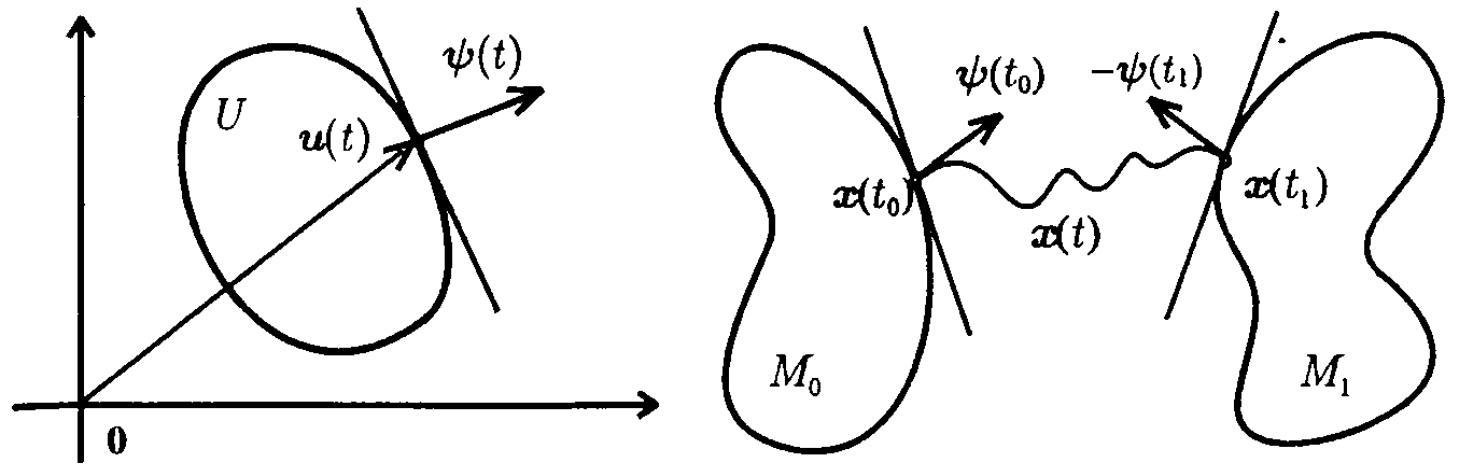
\includegraphics[max width=1.0\textwidth]{images/bo_d547okref24c73bgfch0_124_0_0_1460_467_0.jpg}
\end{center}
\hspace*{3em} 

Рис. 37

Рис. 38

Приведем два утверждения, эквивалентных принципу мак- симума.

Лемма об эквивалентной формулировке принципа максимума Понтрягина. Пусть допустимое управление \(\mathbf{u}\left( t\right)  \in  U,t \in  \left\lbrack  {{t}_{0},{t}_{1}}\right\rbrack  ,\max {o\text{ в }\text{ о }},\) что соответствующее реше- ние xt() системы уравнений (9.1) удовлетворяет граничным условиям х \(\left( {t}_{0}\right)  \in  {M}_{0},x\left( {t}_{1}\right)  \in  {M}_{1}\) . Пусть,далее, \(\psi \left( t\right)  -\) неко- торое решение сопряженной системы уравнений (9.6). Тогда следующие три утверждения эквивалентны:

1) пара и(t), х(t) удовлетворяет принципу максимума с со- пряженной функцией \(\psi \left( t\right)\) на отрезке времени \(I = \left\lbrack  {{t}_{0},{t}_{1}}\right\rbrack\) ;

2) при всех t ∈ I вектор ψ(t) является опорным вектором к множеству достижимости \(X\left( t\right)\) в точке х(н), т.е. выпол- няется равенство

\[
\langle \mathbf{x}\left( t\right) ,\psi \left( t\right) \rangle  = c\left( {X\left( t\right) ,\psi \left( t\right) }\right) . \tag{9.12}
\]

Кроме того, выполнено условие трансверсальности на мно- жестве \({M}_{1}\left( {9.9}\right)\) ;

3) при всех t ∈ I вектор — \(\kappa\) множеству управляемости \(Y\left( t\right)\) в точке х(t), т.е. выполня- ется равенство

\[
\langle \mathbf{x}\left( t\right) , - \psi \left( t\right) \rangle  = c\left( {Y\left( t\right) , - \psi \left( t\right) }\right) . \tag{9.13}
\]

Кроме того, выполнено условие трансверсальности на мно- жестве \({M}_{0}\) (9.8).

Доказательство. Решение х(t) уравнения (9.1) с допус- тимым управлением и(t) запишем в виде формулы Коши с на- чальными условиями в моменты времени но и и (см. формулы (6.7) и (6.9) из лекции 6):

\[
\mathbf{x}\left( t\right)  = {e}^{\left( {t - {t}_{0}}\right) A}\mathbf{x}\left( {t}_{0}\right)  + {\int }_{{t}_{0}}^{t}{e}^{\left( {t - s}\right) A}\mathbf{u}\left( s\right) {ds}; \tag{9.14}
\]

\[
\mathbf{x}\left( t\right)  = {e}^{\left( {t - {t}_{1}}\right) A}\mathbf{x}\left( {t}_{1}\right)  - {\int }_{t}^{{t}_{1}}{e}^{\left( {t - s}\right) A}\mathbf{u}\left( s\right) {ds}. \tag{9.15}
\]

Учитывая свойства экспоненциала (см. лекцию 6), из формул (9.10) и (9.14) получаем выражение

\[
\langle \mathbf{x}\left( t\right) ,\mathbf{\psi }\left( t\right) \rangle  = \left\langle  {{e}^{\left( {t - {t}_{0}}\right) A}\mathbf{x}\left( {t}_{0}\right) ,{e}^{\left( {t - {t}_{0}}\right) {A}^{ * }}\mathbf{\psi }\left( {t}_{0}\right) }\right\rangle   +
\]

\[
+ {\int }_{{t}_{0}}^{t}\left\langle  {{e}^{\left( {t - s}\right) A}\mathbf{u}\left( s\right) ,{e}^{\left( {{t}_{0} - t}\right) {A}^{ * }}\mathbf{\psi }\left( {t}_{0}\right) }\right\rangle  {ds} =
\]

\[
= \left\langle  {\mathbf{x}\left( {t}_{0}\right) ,\mathbf{\psi }\left( {t}_{0}\right) }\right\rangle   + {\int }_{{t}_{0}}^{t}\left\langle  {\mathbf{u}\left( s\right) ,{e}^{\left( {{t}_{0} - s}\right) {A}^{ * }}\mathbf{\psi }\left( {t}_{0}\right) }\right\rangle  {ds} =
\]

\[
= \left\langle  {\mathbf{x}\left( {t}_{0}\right) ,\psi \left( {t}_{0}\right) }\right\rangle   + {\int }_{{t}_{0}}^{t}\langle \mathbf{u}\left( s\right) ,\psi \left( s\right) \rangle {ds}. \tag{9.16}
\]

Аналогично из формул (9.11) и (9.15) получаем выражение

\[
\langle \mathbf{x}\left( t\right) , - \psi \left( t\right) \rangle  = \left\langle  {\mathbf{x}\left( {t}_{1}\right) , - \psi \left( {t}_{1}\right) }\right\rangle   + {\int }_{t}^{{t}_{1}}\langle \mathbf{u}\left( s\right) ,\psi \left( s\right) \rangle {ds}. \tag{9.17}
\]

В лекции 7 были получены опорные функции множеств дости- жимости \(X\left( t\right)\) и управляемости \(Y\left( t\right)\) :

\[
c\left( {X\left( t\right) ,\psi }\right)  = c\left( {{M}_{0},{e}^{\left( {t - {t}_{0}}\right) {A}^{ * }}\psi }\right)  + {\int }_{{t}_{0}}^{t}c\left( {U,{e}^{\left( {t - s}\right) {A}^{ * }}\psi }\right) {ds}; \tag{9.18}
\]

\[
c\left( {Y\left( t\right) ,\psi }\right)  = c\left( {{M}_{1},{e}^{\left( {t - {t}_{1}}\right) {A}^{ * }}\psi }\right)  + {\int }_{t}^{{t}_{1}}c\left( {U, - {e}^{\left( {t - s}\right) {A}^{ * }}\psi }\right) {ds}. \tag{9.19}
\]

Подставляя в формулу (9.18) вместо вектора ф при каждом \(t \in  I\) вектор \(\psi \left( t\right)\) ,заданный формулой (9.10), noлучаем соотношение

\[
c\left( {X\left( t\right) ,\psi \left( t\right) }\right)  = c\left( {{M}_{0},{e}^{\left( {t - {t}_{0}}\right) {A}^{ * }}{e}^{\left( {{t}_{0} - t}\right) {A}^{ * }}\psi \left( {t}_{0}\right) }\right)  +
\]

\[
+ {\int }_{{t}_{0}}^{t}c\left( {U,{e}^{\left( {t - s}\right) {A}^{ * }}{e}^{\left( {{t}_{0} - t}\right) {A}^{ * }}\psi \left( {t}_{0}\right) }\right) {ds} =
\]

\[
= c\left( {{M}_{0},\psi \left( {t}_{0}\right) }\right)  + {\int }_{{t}_{0}}^{t}c\left( {U,{e}^{\left( {{t}_{0} - s}\right) {A}^{ * }}\psi \left( {t}_{0}\right) }\right) {ds} =
\]

\[
= c\left( {{M}_{0},\psi \left( {t}_{0}\right) }\right)  + {\int }_{{t}_{0}}^{t}c\left( {U,\psi \left( s\right) }\right) {ds}. \tag{9.20}
\]

Аналогично, подставляя в формулу (9.19) вектор — ный формулой (9.11), получаем соотношение

\[
c\left( {Y\left( t\right) , - \psi \left( t\right) }\right)  = c\left( {{M}_{1}, - \psi \left( {t}_{1}\right) }\right)  + {\int }_{t}^{{t}_{1}}c\left( {U,\psi \left( s\right) }\right) {ds}. \tag{9.21}
\]

Докажем теперь эквивалентность утверждений 1 — 3. Пусть пара и(t), х(t) удовлетворяет принципу максимума на отрезке времени \(\left\lbrack  {{t}_{0},{t}_{1}}\right\rbrack\) . Из условия максимума (9.7) и условия транс- версальности на множестве \({M}_{0}\) (9.8) следует,что правые части выражений (9.16) и (9.20) совпадают. Таким образом, выпол- няется равенство (9.12). Аналогично из формул (9.7) и (9.9) следует, что правые части выражений (9.17) и (9.21) совпадают. Таким образом, выполняется равенство (9.13). Следовательно, из утверждения 1 получаем 2 и 3.

Пусть выполнено утверждение 2. Из равенства (9.12) при \(t = {t}_{1}\) получаем соотношение

\[
c\left( {X\left( {t}_{1}\right) ,\psi \left( {t}_{1}\right) }\right)  - \left\langle  {\mathbf{x}\left( {t}_{1}\right) ,\psi \left( {t}_{1}\right) }\right\rangle   = 0.
\]

Используя формулы (9.20)и (9.16),преобразуем егоквиду

\[
\left\lbrack  {c\left( {{M}_{0},\psi \left( {t}_{0}\right) }\right)  - \left\langle  {\mathbf{x}\left( {t}_{0}\right) ,\psi \left( {t}_{0}\right) }\right\rangle  }\right\rbrack   + {\int }_{{t}_{0}}^{{t}_{1}}\left\lbrack  {c\left( {U,\psi \left( s\right) }\right)  - \langle \mathbf{u}\left( s\right) ,\psi \left( s\right) \rangle }\right\rbrack  {ds} = 0.
\]

(9.22)

Из включений \(\mathbf{x}\left( {t}_{0}\right)  \in  {M}_{0}\) и \(\mathbf{u}\left( t\right)  \in  U\) при всех t ∈ \(I\) corласно свойствам опорных функций следует, что первое слагаемое в формуле (9.22) неотрицательно, подынтегральная функция так- же неотрицательна, значит, и интеграл неотрицателен. Таким образом, из равенства (9.22) получаем следующие равенства:

\[
c\left( {{M}_{0},\psi \left( {t}_{0}\right) }\right)  - \left\langle  {\mathbf{x}\left( {t}_{0}\right) ,\psi \left( {t}_{0}\right) }\right\rangle   = 0,
\]

\[
{\int }_{{t}_{0}}^{{t}_{1}}\left\lbrack  {c\left( {U,\psi \left( s\right) }\right) -\langle \mathbf{u}\left( s\right) ,\psi \left( s\right) \rangle }\right\rbrack  {ds} = 0
\]

Из первого равенства вытекает условие трансверсальности на множестве \({M}_{0}\left( {9.8}\right)\) , a из второго, с учетом неотрицательнос- ти подынтегральной функции и свойства 6 интеграла Лебега (раздел Д6 дополнений) — условие максимума (9.7) при почти всех t ∈ \(\left\lbrack  {{t}_{0},{t}_{1}}\right\rbrack\) . Следовательно, из утверждения 2 получается утверждение 1.

Аналогично из утверждения 3 следует утверждение 1. Дей- ствительно, из равенства (9.13) при \(t = {t}_{0}\) получаем соотно- шение

\[
c\left( {Y\left( {t}_{0}\right) , - \psi \left( {t}_{0}\right) }\right)  - \left\langle  {\mathbf{x}\left( {t}_{0}\right) , - \psi \left( {t}_{0}\right) }\right\rangle   = 0.
\]

Используяформулы (9.21)и (9.17),преобразуем егоквиду

\[
\left\lbrack  {c\left( {{M}_{1}, - \psi \left( {t}_{1}\right) }\right)  - \left\langle  {\mathbf{x}\left( {t}_{1}\right) , - \psi \left( {t}_{1}\right) }\right\rangle  }\right\rbrack   +
\]

\[
+ {\int }_{{t}_{0}}^{{t}_{1}}\left\lbrack  {c\left( {U,\psi \left( s\right) }\right) -\langle \mathbf{u}\left( s\right) ,\mathbf{\psi }\left( s\right) \rangle }\right\rbrack  {ds} = 0. \tag{9.23}
\]

Из включений х \(\left( {t}_{1}\right)  \in  {M}_{1}\) и и \(u\left( t\right)  \in  U\) получаем,что оба сла- гаемые в формуле (9.23) неотрицательны, следовательно, рав- ны нулю. Первое слагаемое дает условие трансверсальности на множестве \({M}_{1}\left( {9.9}\right)\) , a второе — условие максимума (9.7) при почти всех t ∈ I.

Таким образом, лемма полностью доказана.

Замечание. Из приведенного доказательства видно, что в утверждении 2 достаточно потребовать, чтобы вектор \(\mathbf{\psi }\left( t\right)\) был опорным к множеству достижимости \(X\left( t\right)\) в точке х(t) лишь при \(t = {t}_{1}\) , т.е. чтобы равенство (9.12) выполнялось только в конечный момент времени \(t = {t}_{1}\) . Тогда выполняется утвержде- ние 1 и, следовательно, равенство (9.12) выполняется при всех \(t \in  \left\lbrack  {{t}_{0},{t}_{1}}\right\rbrack\) .

Доказанная выше лемма позволяет придать принципу максимума Понтрягина следу- ющий геометрический смысл. Если пара и(t), х(t) удовле- творяет принципу максимума на отрезке времени \(\left\lbrack  {{t}_{0},{t}_{1}}\right\rbrack\) c сопряженной функцией ф \(\psi \left( t\right)\) , то в каждый момент времени \(t \in  \left\lbrack  {{t}_{0},{t}_{1}}\right\rbrack\) ruпeрплоскость

\[
{\Gamma }_{\psi \left( t\right) } = \left\{  {\mathbf{x} \in  {E}^{n} : \langle \mathbf{x},\psi \left( t\right) \rangle  = \langle \mathbf{x}\left( t\right) ,\psi \left( t\right) \rangle }\right\}  ,
\]

\begin{center}
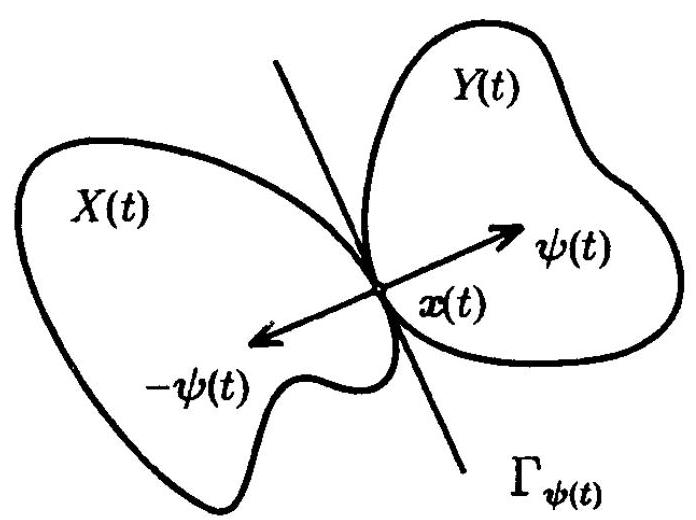
\includegraphics[max width=0.6\textwidth]{images/bo_d547okref24c73bgfch0_128_765_9_696_520_0.jpg}
\end{center}
\hspace*{3em} 

Рис. 39

проходящая через точку х (н с вектором нормали ψ(t), разделя- ет множество достижимости \(X\left( t\right)\) и множество управляемости \(Y\left( t\right)\) (puc. 39).

\section*{9.3. Необходимые условия оптимальности}

Рассмотрим, при каких предположениях принцип макси- мума Понтрягина является необходимым условием оптималь- ности.

Теорема о необходимых условиях оптимальности. Пусть в задаче быстродействия множества М0 и М1 выпук- лы. Пусть, далее, и(t) — оптимальное управление, переводя- щее объект из множества М0 на множество М1 на отрез- ке времени I = [t,1,1], \(u\mathbf{x}\left( t\right)  -\) coomвemcтвующее решение уравнения (9.1). Тогда пара и(t), х(t) удовлетворяет принципу максимума Понтрягина на отрезке времени I.

Доказательство. Нужно доказать существование такого нетривиального решения сопряженной системы (9.6), что вы- полняются условия (9.7)—(9.9). Управление и(t) по предположе- нию теоремы является оптимальным в задаче быстродействия и переводит объект из начального множества М0 на конечное множество \({M}_{1}\) на отрезке времени [ \({t}_{0},{t}_{1}\) ]. Cледовательно, мно- жество достижимости \(X\left( t\right)\) для любого момента времени t < \({t}_{1}\) удовлетворяет соотношениям

\[
X\left( {t}_{1}\right)  \cap  {M}_{1} \neq  \varnothing ,\;X\left( t\right)  \cap  {M}_{1} = \varnothing . \tag{9.24}
\]

Paccmorphm функцию

\[
\varphi \left( {t,\psi }\right)  = c\left( {X\left( t\right) ,\psi }\right)  + c\left( {{M}_{1}, - \psi }\right) \tag{9.25}
\]

и последовательность точек \({t}_{k} = {t}_{1} - \frac{1}{k} < {t}_{1}\) . Множества М0 и \({M}_{1}\) выпуклы по предположению теоремы, и множество дости- жимости \(X\left( t\right)\) выпукло согласно свойству 3 множеств достижи- мости (см. лекцию 7). В этом случае соотношения (9.24) можно в эквивалентном виде записать с помощью опорных функций. Используя следствие из свойства 12 опорных функций (см. лек- цию 3), получим следующее утверждение: для любого вектора \(\psi  \in  S\) выполняется неравенство

\[
\varphi \left( {{t}_{1},\psi }\right)  = c\left( {X\left( {t}_{1}\right) ,\psi }\right)  + c\left( {{M}_{1}, - \psi }\right)  \geq  0 \tag{9.26}
\]

и для любого \({t}_{k} < {t}_{1}\) существует вектор \({\psi }_{k} \in  S\) такой,что справедливо строгое неравенство

\[
\varphi \left( {{t}_{k},{\psi }_{k}}\right)  = c\left( {X\left( {t}_{k}\right) ,{\psi }_{k}}\right)  + c\left( {{M}_{1}, - {\psi }_{k}}\right)  < 0. \tag{9.27}
\]

Векторы \({\psi }_{k}\) принадлежат компактному множеству \(S\) ,поэтому из последовательности \(\left\{  {\psi }_{k}\right\}\) можно выбрать подпоследователь- ность, сходящуюся к некоторому вектору фе S. Обозначим ее снова через \(\left\{  {\psi }_{k}\right\}\) . Функция \(\varphi \left( {t,\psi }\right)\) непрерывна по \(\psi\) как сумма двух непрерывных опорных функций (см. следствие из свойства 13 опорных функций, лекция 3). Более того, функция \(\varphi \left( {t,\psi }\right)\) непрерывна по \(t\) ,так как множество достижимости \(X\left( t\right)\) непрерывно зависит от t (см. свойство 7 из лекции 7) и опорная функция \(c\left( {X\left( t\right) ,\mathbf{\psi }}\right)\) является непрерывной по t в силу следствия из свойства 13 опорных функций.

Таким образом, в неравенстве (9.27) можно перейти к преде- лу при \(k \rightarrow  \infty\) . Поскольку \({t}_{k} \rightarrow  {t}_{1}\) и \({\psi }_{k} \rightarrow  \overline{\psi }\) ,в пределе получим неравенство

\[
\varphi \left( {{t}_{1},\overline{\psi }}\right)  \leq  0
\]

Отсюда,учитывая неравенство (9.26),получаем равенство

\[
\varphi \left( {{t}_{1},\overline{\psi }}\right)  = 0,
\]

а по определению функции \(\varphi \left( {t,\psi }\right)\) (см. формулу (9.25)) это озна- чает, что для вектора ψ с ∈ S справедливо соотношение

\[
c\left( {X\left( t\right) ,\overline{\psi }}\right)  + c\left( {{M}_{1}, - \overline{\psi }}\right)  = 0. \tag{9.28}
\]

Поскольку точка x(t1) принадлежит обоим множествам X(t1) и \({M}_{1}\) ,имеем следующие неравенства (см. следствие из свойства 6 опорных функций, лекция 3):

\[
\left\langle  {\mathbf{x}\left( {t}_{1}\right) ,\overline{\mathbf{\psi }}}\right\rangle   \leq  c\left( {X\left( {t}_{1}\right) ,\overline{\mathbf{\psi }}}\right)
\]

\[
\langle \mathbf{x}\left( {t}_{1}\right) , - \overline{\mathbf{\psi }}\rangle  \leq  c\left( {{M}_{1}, - \overline{\mathbf{\psi }}}\right) .
\]

В действительности в этих неравенствах выполняется равенст- во, так как если хотя бы в одном из них есть строгое неравен- ство, то, складывая их, получим строгое неравенство

\[
0 < c\left( {X\left( {t}_{1}\right) ,\overline{\psi }}\right)  + \mathrm{c}\left( {{M}_{1}, - \overline{\psi }}\right) ,
\]

а это противоречит равенству (9.28). Таким образом, имеем два равенства:

\[
\langle \mathbf{x}\left( {t}_{1}\right) ,\overline{\psi }\rangle  = c\left( {X\left( {t}_{1}\right) ,\overline{\psi }}\right) , \tag{9.29}
\]

\[
\left\langle  {\mathbf{x}\left( {t}_{1}\right) , - \overline{\mathbf{\psi }}}\right\rangle   = c\left( {{M}_{1}, - \overline{\mathbf{\psi }}}\right) . \tag{9.30}
\]

Рассмотрим решение ψ(t) сопряженной системы дифферен- циальных уравнений (9.6) с начальным условием в точке и, а именно, \(\mathbf{\psi }\left( {t}_{1}\right)  = \overline{\mathbf{\psi }}\) . Эта сопряженная функция задается форму- лой (9.11). Она невырожденна, так как тр и 90 мектор и принад- лежит единичной сфере \(S\) ). Учитывая равенство ψ(1) = 1 , из формулы (9.30) получаем условия трансверсальности на мно- жестве \({M}_{1}\left( {9.9}\right)\) , a из формулы (9.29) — развество (9.12) при t = t1. Таким образом, справедливо утверждение 2 леммы об эквивалентной формулировке принципа максимума Понтряги- на (см. сделанное выше замечание). По лемме пара и(t), х(t) удовлетворяет принципу максимума на отрезке времени [t, t] ссопряженной функцией \(\mathbf{\psi }\left( t\right)\) . Тем самым теорема доказана.

\section*{ЛЕКЦИЯ 10}

\begin{itemize}\relax
\item\relax Схема применения принципа максимума Понтрягина для решения линейной задачи быстродействия.
\end{itemize}

\begin{itemize}\relax
\item\relax Примеры.
\end{itemize}

\section*{10.1. Применение необходимых условий оптимальности}

Рассмотрим снова линейную задачу быстродействия. Она заключается в нахождении допустимого управления \(\mathbf{u}\left( t\right)  \in  U\) , переводящего объект, описываемый уравнением

\[
\dot{x} = {Ax} + u, \tag{10.1}
\]

из начального множества М0 на конечное множество \({M}_{1}\) за наи- меньшее время. Допустимым управлением является произволь- ная измеримая функция \(u\left( t\right)  \in  U\) ,множества \({M}_{0},{M}_{1},U \in  {E}^{n}\) предполагаются непустыми и компактными.

Для этой задачи в предыдущей лекции была доказана теоре- ма о необходимых условиях оптимальности. Для случая, когда множества \({M}_{0}\) и \({M}_{1}\) выпуклы,эта теорема утверждает,что любая пара и(t), х(t), решающая задачу оптимального быстро- действия на отрезке времени \(I = \left\lbrack  {{t}_{0},{t}_{1}}\right\rbrack\) ,должна удовлетворять на этом отрезке времени принципу максимума Понтрягина. По определению пара \(\mathbf{u}\left( t\right) ,\mathbf{x}\left( t\right)\) удовлетворяет принципу максимума на отрезке [t, t, н сли существует такое нетривиальное реше- ние \(\psi \left( t\right)\) вспомогательной сопряженной системы

\[
\dot{\psi } =  - {A}^{ * }\psi , \tag{10.2}
\]

что выполнены следующие три условия:

1) условие максимума

\[
\langle \mathbf{u}\left( t\right) ,\mathbf{\psi }\left( t\right) \rangle  = c\left( {U,\mathbf{\psi }\left( t\right) }\right) \tag{10.3}
\]

для почти всех t ∈ I;

2) условие трансверсальности на множестве \({M}_{0}\)

\[
\left\langle  {\mathbf{x}\left( {t}_{0}\right) ,\mathbf{\psi }\left( {t}_{0}\right) }\right\rangle   = c\left( {{M}_{0},\mathbf{\psi }\left( {t}_{0}\right) }\right) ; \tag{10.4}
\]

3) условие трансверсальности на множестве М1

\[
\left\langle  {\mathbf{x}\left( {t}_{1}\right) , - \psi \left( {t}_{1}\right) }\right\rangle   = c\left( {{M}_{1}, - \psi \left( {t}_{1}\right) }\right) . \tag{10.5}
\]

Таким образом, для решения задачи быстродействия можно поступить следующим образом. Найти все управления, удов- летворяющие принципу максимума Понтрягина, а затем среди этого множества управлений каким-либо образом найти дейст- вительно оптимальное управление. Эффективность такого под- хода определяется тем, как много управлений будет удовлетво- рять принципу максимума. Чем уже множество таких управ- лений, тем проще выбрать из него действительно оптимальное управление. Оказывается, что принцип максимума Понтряги- на в этом смысле является довольно эффективным средством решения линейных задач быстродействия.

Заметим, что если сопряженная функция \(\mathbf{\psi }\left( t\right)\) является ре- шением линейной системы уравнений (10.2) и удовлетворяет равенствам (10.3)—(10.5), то функция \(\lambda \mathbf{\psi }\) , где λ — произволь- ное неотрицательное число, также является решением системы (10.2) и удовлетворяет равенствам (10.3)—(10.5). Это следует из того факта, что система уравнений (10.2) линейна и однородна, а опорные функции в равенствах (10.3)-(10.5) положительно од- нородны (см. свойство 1 опорных функций из лекции 3). Таким образом, при отыскании сопряженных функций ψ(t), удовлетво- ряющих принципу максимума Понтрягина, можно нормировать эти функции в какой-нибудь момент времени, например при \(t = {t}_{0},\left\lVert \begin{array}{c} {\psi \left( {t}_{0}\right) } \end{array} \right\rVert = 1\) ,и перебирать сопряженные функции \(\psi \left( t\right)\) с начальными условиями из единичной сферы, \(\mathbf{\psi }\left( {t}_{0}\right)  \in  S\) .

Рассмотрим, как построить все управления, удовлетворяю- щие принципу максимума. Для этого можно предложить следу- ющую схему (рис. 40). Начальный момент времени и в нашей задаче зафиксирован. Возьмем произвольный начальный вектор \(\psi \left( {t}_{0}\right)\) из единичной сферы \(S \subset  {E}^{n}\) . Найдем решение ψ(t) co- пряженной системы (10.2) с этим начальным значением ψ(0). В силу теоремы 1 (см. лекцию 6) это решение ψ(t) сущест- вует и единственно на любом отрезке времени \(\left\lbrack  {{t}_{0},{t}_{1}}\right\rbrack  ,{t}_{1} \geq  {t}_{0}\) . Факт единственности этого решения показан на схеме одинар- ной стрелкой. Далее, зная решение ψ(t) сопряженной системы, найдем все допустимые управления \(\mathbf{u}\left( t\right)  \in  U\) , yдовлетворяю- щие условию максимума (10.3). Таких управлений и(t) может быть несколько, и это указано на схеме двойной стрелкой. В дальнейшем (см. лекцию 12) исследуем, при каких условиях такое управление и(t) определяется по функции ψ(t) однознач- ным образом. По данному же начальному вектору ф(и) найдем все начальные значения вектора фазового состояния объекта \(\mathbf{x}\left( {t}_{0}\right)\) из начального множества М0, удовлетворяющие условию трансверсальности на множестве М0 (10.4). Таких начальных значений \(x\left( {t}_{0}\right)\) опять может быть несколько. Этот факт также показан на схеме двойной стрелкой. В дальнейшем (см. лек- цию 12) исследуем, при каких условиях вектор х(но) определя- ется однозначным образом по вектору \(\mathbf{\psi }\left( {t}_{0}\right)\) . Теперь, зная до- пустимое управление и(t) и начальное состояние объекта х(t0), найдем решение уравнения (10.1). Это решение х(t) в силу те- оремы 1 (см. лекцию 6) находится однозначно по функции и(t) и начальному условию х(t0). Πосле того как построено решение \(\mathbf{x}\left( t\right)\) , ocталось только проверить, достигнет ли это решение при каком-либо \({t}_{1} \geq  {t}_{0}\) множества \({M}_{1}\) или нет, a если решение х достигнет в какой-то момент \({t}_{1}\) множества \({M}_{1}\) , to выполняется ли условие трансверсальности на множестве М1 (10.5). Если это условие выполнено, то пара и(t), х(t) удовлетворяет принципу максимума Понтрягина на полученном отрезке времени [t, t, i]; если это условие не выполнено, то пара и(t), х(t) не удовлетво- ряет принципу максимума.

\begin{center}
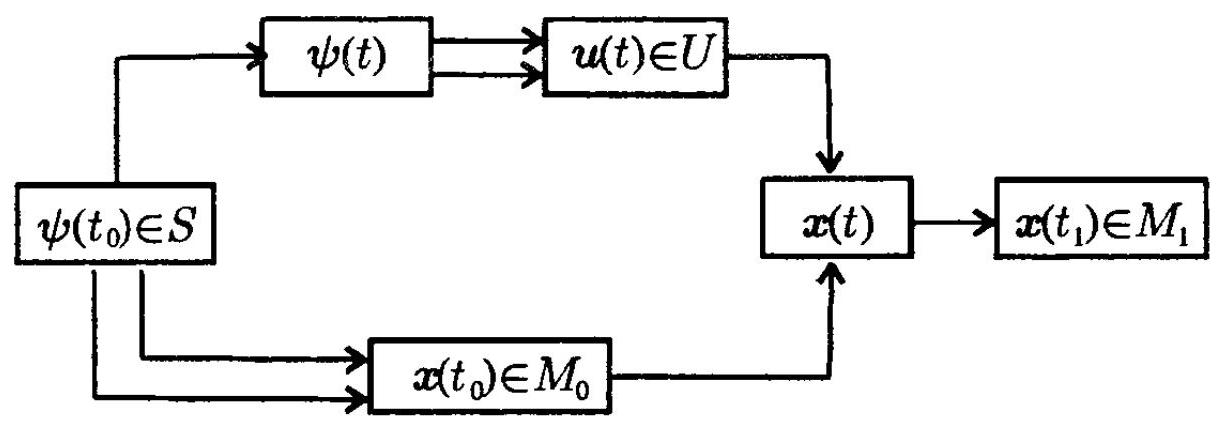
\includegraphics[max width=1.0\textwidth]{images/bo_d547okref24c73bgfch0_133_142_0_1223_424_0.jpg}
\end{center}
\hspace*{3em} 

Рис. 40

Заметим, что при таком подходе все пары и(t), х(t), удовле- творяющие принципу максимума, зависят лишь от начального вектора \(\psi \left( {t}_{0}\right)  \in  S\) , причем эта зависимость на двух этапах может быть неоднозначной. В дальнейшем (см. лекцию 12) по- кажем, что при некоторых дополнительных условиях на задачу быстродействия эта зависимость однозначна. Заметим также, что если известно, что объект является управляемым из мно- жества \({M}_{0}\) на множество \({M}_{1}\) на отрезке времени \(\left\lbrack  {{t}_{0},{t}_{1}}\right\rbrack\) , to pe- шения \(\mathbf{\psi }\left( t\right)\) и \(\mathbf{x}\left( t\right)\) в данной схеме можно строить лишь на этом отрезке времени.

Проиллюстрируем данную схему решения задачи быстро- действия на конкретных примерах.

Пример 1. Рассмотрим задачу под условным названием "Запуск ракеты с Земли на космическую станцию". Пусть ра- кета единичной массы движется прямолинейно в соответствии с законом движения

\[
\ddot{x} = f\left( t\right) ,
\]

где х — отклонение ракеты от какой-либо фиксированной точки, \(\ddot{x}\) - ускорение ракеты, \(f\left( t\right)\) - сила, действующая на ракету в момент времени t. Предполагается, что силу f(t) можно изме- нять со временем в пределах возможностей двигателя ракеты, которые определяются условием \(\left| {f\left( t\right) }\right|  \leq  1\) . В начальный момент времени \({t}_{0} = 0\) pakera находится в состоянии \(x\left( 0\right)  =  - \frac{5}{2}\) . При этом можно также придать ракете ограниченную начальную скорость \(\left| {\dot{x}\left( 0\right) }\right|  \leq  1\) . Tpeбуется за наименьшее время перевести ракету в состояние \(1 \leq  x\left( {t}_{1}\right)  \leq  2,\dot{x}\left( {t}_{1}\right)  = 0\) ,т.е. с нулевой ско- ростью произвести стыковку с космической станцией, которая может подойти в любое из положений \(1 \leq  x \leq  2\) к заданному моменту времени.

Приведем данную задачу к стандартному виду. Для этого введем новые переменные \({x}^{1} = x,{x}^{2} = \dot{x},{u}^{1} = 0,{u}^{2} = f\) . Таким образом, фазовый вектор объекта является двумерным \(\mathbf{x} = \left( {{\mathbf{x}}^{1},{\mathbf{x}}^{2}}\right)\) , a уравнение движения имеет вид

\[
\left\{  \begin{array}{l} {\dot{x}}^{1} = {x}^{2} \\  {\dot{x}}^{2} = {u}^{2} \end{array}\right. \tag{10.6}
\]

Orpаничение на управление \(u = \left( {{u}^{1},{u}^{2}}\right)\) задается множеством

\[
U = \left\{  {\mathbf{u} \in  {E}^{2} : {u}^{1} = 0,\left| {u}^{2}\right|  \leq  1}\right\}  .
\]

Начальное множество \({M}_{0}\) имеет вид (рис. 41)

\[
{M}_{0} = \left\{  {\mathbf{x} \in  {E}^{2} : {x}^{1} =  - \frac{5}{2},\left| {x}^{2}\right|  \leq  1}\right\}  ,
\]

a конечное множество \({M}_{1} -\) вид

\[
{M}_{1} = \left\{  {\mathbf{x} \in  {E}^{2} : 1 \leq  {x}^{1} \leq  2,{x}^{2} = 0}\right\}  .
\]

\begin{center}
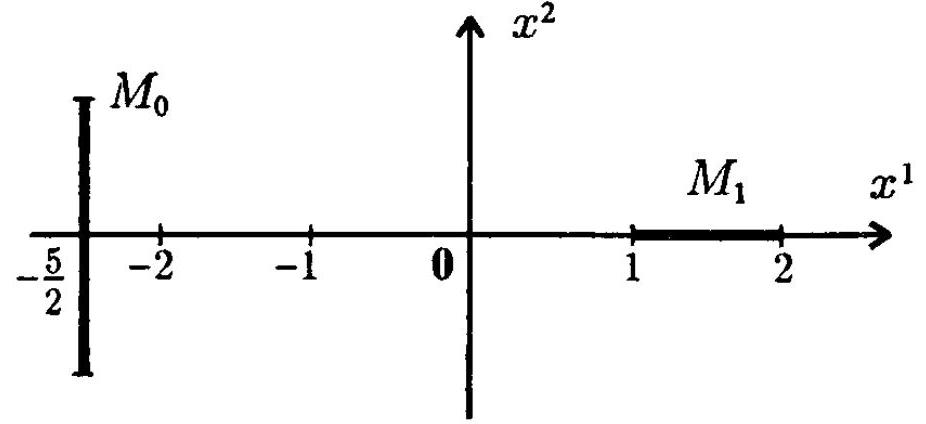
\includegraphics[max width=0.8\textwidth]{images/bo_d547okref24c73bgfch0_135_276_0_926_424_0.jpg}
\end{center}
\hspace*{3em} 

Рис. 41

Найдем все управления, удовлетворяющие принципу макси- мума Понтрягина, для чего запишем все условия этого принци- па применительно к данной задаче. Матрица А для уравнения (10.6) имеет вид \(A = \left( \begin{array}{ll} 0 & 1 \\  0 & 0 \end{array}\right)\) . Cледовательно, \({A}^{ * } = \left( \begin{array}{ll} 0 & 0 \\  1 & 0 \end{array}\right)\) и сопряженная система уравнений (10.2) принимает вид

\[
\left\{  \begin{array}{l} {\dot{\psi }}^{1} = 0 \\  {\dot{\psi }}^{2} =  - {\psi }^{1} \end{array}\right. \tag{10.7}
\]

Опорные функции множеств U, М0, М1 вычисляются непосред- ственно:

\[
c\left( {U,\psi }\right)  = \left| {\psi }^{2}\right| ,\;c\left( {{M}_{0},\psi }\right)  =  - \frac{5}{2}{\psi }^{1} + \left| {\psi }^{2}\right| ,\;c\left( {{M}_{1},\psi }\right)  = \frac{3}{2}{\psi }^{1} + \frac{1}{2}\left| {\psi }^{1}\right| .
\]

Изусловия максимума (10.3) получаем равенство

\[
{u}^{2}\left( t\right) {\psi }^{2}\left( t\right)  = \left| {{\psi }^{2}\left( t\right) }\right|
\]

следовательно, имеем соотношения

\[
{u}^{2}\left( t\right)  =  + 1\text{ ,если }{\psi }^{2}\left( t\right)  > 0\text{ , }
\]

\[
{u}^{2}\left( t\right)  =  - 1\text{ ,если }{\psi }^{2}\left( t\right)  < 0, \tag{10.8}
\]

\[
- 1 \leq  {u}^{2}\left( t\right)  \leq  1,\;\text{ если }\;{\psi }^{2}\left( t\right)  = 0.
\]

Из условия трансверсальности на множестве Мо (10.4) получаем равенство

\[
- \frac{5}{2}{\psi }^{1}\left( 0\right)  + {x}^{2}\left( 0\right) {\psi }^{2}\left( 0\right)  =  - \frac{5}{2}{\psi }^{1}\left( 0\right)  + \left| {{\psi }^{2}\left( 0\right) }\right| ,
\]

следовательно, справедливы соотношения

\[
{x}^{2}\left( {t}_{0}\right)  =  + 1,\;\text{ если }\;{\psi }^{2}\left( 0\right)  > 0,
\]

\[
{x}^{2}\left( {t}_{0}\right)  =  - 1,\;\text{ если }\;{\psi }^{2}\left( 0\right)  < 0, \tag{10.9}
\]

\[
- 1 \leq  {x}^{2}\left( {t}_{0}\right)  \leq   + 1,\;\text{ если }\;{\psi }^{2}\left( 0\right)  = 0.
\]

И наконец, из условия трансверсальности на множестве М1 (10.5) получаем равенство

\[
{x}^{1}\left( {t}_{1}\right) \left( {-{\psi }^{1}\left( {t}_{1}\right) }\right)  =  - \frac{3}{2}{\psi }^{1}\left( {t}_{1}\right)  + \frac{1}{2}\left| {{\psi }^{1}\left( {t}_{1}\right) }\right| ,
\]

следовательно, выполняются соотношения

\[
{x}^{1}\left( {t}_{1}\right)  = 1,\;\text{ если }\;{\psi }^{1}\left( {t}_{1}\right)  > 0,
\]

\[
{x}^{1}\left( {t}_{1}\right)  = 2,\;\text{ если }\;{\psi }^{1}\left( {t}_{1}\right)  < 0, \tag{10.10}
\]

\[
1 \leq  {x}^{1}\left( {t}_{1}\right)  \leq  2,\;\text{ если }\;{\psi }^{1}\left( {t}_{1}\right)  = 0.
\]

Рассмотрим решение сопряженной системы (10.7) с началь- ным условием \(\psi \left( 0\right)  = \left( {{\psi }^{1}\left( 0\right) ,{\psi }^{2}\left( 0\right) }\right)  \in  S\) . Это решение имеет вид

\[
{\psi }^{1}\left( t\right)  \equiv  {\psi }^{1}\left( 0\right) ,\;{\psi }^{2}\left( t\right)  =  - {\psi }^{1}\left( 0\right) t + {\psi }^{2}\left( 0\right) .
\]

Из условия максимума (10.8) следует, что управление \({u}^{2}\left( t\right)\) , удовлетворяющее принципу максимума, зависит от знака функ- ции \({\psi }^{2}\left( t\right)\) (рис. 42). Для тех моментов времени \(t\) , для которых \({\psi }^{2}\left( t\right)  > 0\) , управление имеет вид \({u}^{2}\left( t\right)  =  + 1\) , а для тех моментов времени \(t\) , для которых \({\psi }^{2}\left( t\right)  < 0\) , управление имеет вид \({u}^{2}\left( t\right)  =  - 1\) . Если в какой-то момент времени \(\theta\) функция \({\psi }^{2}\left( t\right)\) обращается в нуль, то в этот момент времени управление \({u}^{2}\left( \theta \right)\) из условия максимума не определя- ется. Оно может принимать произ- вольное значение \(- 1 \leq  {u}^{2}\left( \theta \right)  \leq   + 1\) . Функция \({\psi }^{2}\left( t\right)\) линейно зависит от времени \(t\) и не может тождествен- но обращаться в нуль, поскольку \(\parallel \mathbf{\psi }\left( 0\right) \parallel  = 1\) . Таким образом, функ- ция \({\psi }^{2}\left( t\right)\) может обращаться в нуль не более чем в одной точке. Следо- вательно, управление \({u}^{2}\left( t\right)\) , удов- летворяющее условию максимума (10.8), является кусочно постоян- ным, принимающим лишь два зна- чения \(+1\) и \(-1\) , причем оно может менять свое значение не бо- лее одного раза именно в тот момент времени \(\theta\) , ког- да \({\psi }^{2}\left( \theta \right)  = 0\) (см. рис. 42). Произвол в выборе управле- ния \({u}^{2}\left( t\right)\) в одной точке \(t = \theta\) никак не сказывается на ре- шении \(\mathbf{x}\left( t\right)\) системы уравне- ний (10.6).

\begin{center}
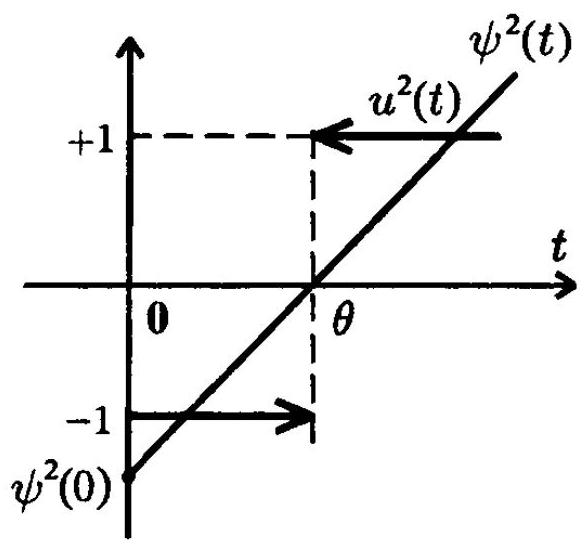
\includegraphics[max width=0.5\textwidth]{images/bo_d547okref24c73bgfch0_136_860_1517_584_549_0.jpg}
\end{center}
\hspace*{3em} 

Рис. 42

\begin{center}
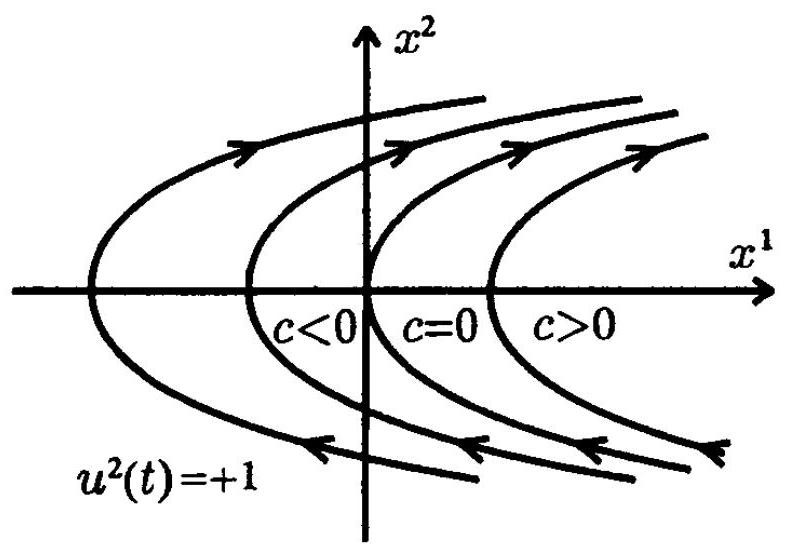
\includegraphics[max width=0.7\textwidth]{images/bo_d547okref24c73bgfch0_137_4_0_785_550_0.jpg}
\end{center}
\hspace*{3em} 

Рис. 43

Выясним, по какой тра- ектории в фазовой плоскос- TH \(x = \left( {{x}^{1},{x}^{2}}\right)\) будет дви- гаться точка х(t) в случае, когда и’(t) = +1. В силу уравнения (10.6) в этом случае имеем соотношения

\[
\left\{  \begin{array}{l} {\dot{x}}^{1} = {x}^{2} \\  {\dot{x}}^{2} = 1 \end{array}\right. \tag{10.11}
\]

Разделив первое уравнение на второе и проинтегрировав, полу- чаем \({x}^{1} = \frac{1}{2}{\left( {x}^{2}\right) }^{2} + c\) ,где \(c\) — постоянная интегрирования, опре- деляемая начальной точкой траектории. Такие фазовые тра- ектории изображены на рис. 43. Они представляют собой се- мейство парабол, направление движения по которым указано стрелками. Такое направление объясняется тем, что \({\dot{x}}^{2} = 1\) ,т.е. координата \({x}^{2}\left( t\right)\) возрастает с течением времени.

Аналогично строят фазовые траектории для случая, когда \({u}^{2}\left( t\right)  =  - 1\) . Они задаются уравнением \({x}^{1} =  - \frac{1}{2}{\left( {x}^{2}\right) }^{2} + c\) . Это семейство парабол изображено на рис. 44.

\begin{center}
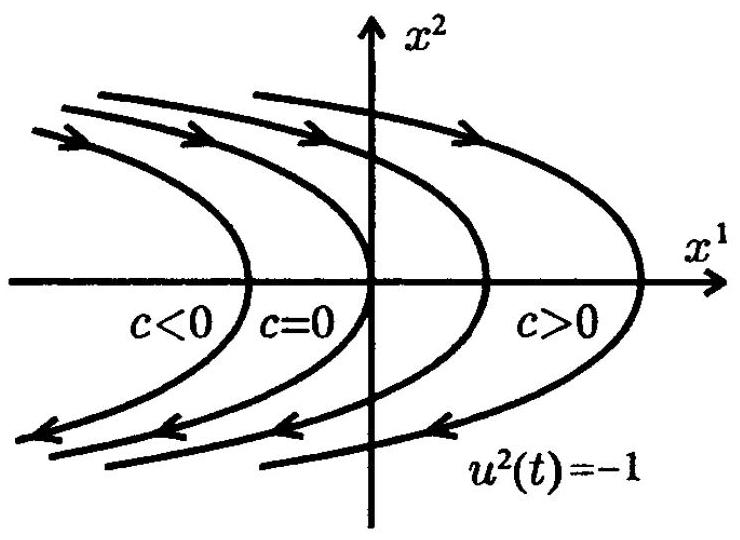
\includegraphics[max width=0.7\textwidth]{images/bo_d547okref24c73bgfch0_137_26_1571_740_540_0.jpg}
\end{center}
\hspace*{3em} 

Рис. 44

Таким образом, в мо- менты времени \(t\) , когда \({u}^{2}\left( t\right)  =  + 1\) , движение фа- зовой точки \(x\left( t\right)\) происхо- дит по траекториям, изоб- раженным на рис. 43, а в моменты времени t, когда \({u}^{2}\left( t\right)  =  - 1\) ,— по траек- ториям, изображенным на рис. 44.

Построим теперь по схе- ме, приведенной на рис. 40, все управления и траекто- рии, удовлетворяющие принципу максимума Понтрягина. Для этого исследуем поведение линейной функции

\[
{\psi }^{2}\left( t\right)  =  - {\psi }^{1}\left( 0\right) t + {\psi }^{2}\left( 0\right) .
\]

Будем выбирать всевозможные начальные значения ( \({\psi }^{1}\left( 0\right)\) , \(\left. {{\psi }^{2}\left( 0\right) }\right)  \in  S\) . Рассмотрим три случая.

Случай 1. Если \({\psi }^{2}\left( 0\right)  < 0\) , то из условия трансверсальнос- ти на множестве \({M}_{0}\) следует, что начальная точка траектории имеет вид \(\mathbf{x}\left( 0\right)  = \left( {-\frac{5}{2}, - 1}\right)\) . Функция \({\psi }^{2}\left( t\right)\) в этом случае может быть отрицательной при всех \(t \geq  0\) , если \({\psi }^{1}\left( 0\right)  > 0\) (прямая I на рис. 45), либо, начиная с некоторого момента времени \(\theta  > 0\) , стать положительной, если \({\psi }^{1}\left( 0\right)  < 0\) (прямая I' на рис. 45). Следовательно, согласно условию максимума (10.8) управление \({u}^{2}\left( t\right)\) будет иметь вид \({u}^{2}\left( t\right)  \equiv   - 1\) , или, начиная с момента вре- мени \(\theta\) , переключается на \(+1\) . В любом случае фазовая траек- тория \(\mathbf{x}\left( t\right)\) , выходящая из точки \(\mathbf{x}\left( 0\right)  = \left( {-\frac{5}{2}, - 1}\right)\) , при таком управлении никогда не достигнет множества \({M}_{1}\) . Полученные траектории обозначены на рис. 46 римскими цифрами I и I' соответственно.

Случай 2. Если \({\psi }^{2}\left( 0\right)  = 0\) , то из соотношения (10.9) сле- дует, что начальная точка \(\mathbf{x}\left( 0\right)\) может принимать произвольное значение из множества \({M}_{0}\) . В этом случае \({\psi }^{1}\left( 0\right)  \neq  0\) , поскольку \(\psi \left( 0\right)  \in  S\) , а функция \({\psi }^{2}\left( t\right)\) либо отрицательна при всех \(t > 0\) , если \({\psi }^{1}\left( 0\right)  > 0\) (прямая II на рис. 45), либо положительна при всех \(t > 0\) , если \({\psi }^{1}\left( 0\right)  < 0\) (прямая II' на рис. 45). В силу условия (10.8) это означает, что управление \({u}^{2}\left( t\right)\) постоянно при всех \(t > 0\) и равно \(-1\) , если \({\psi }^{1}\left( 0\right)  > 0\) , и равно \(+1\) , если \({\psi }^{1}\left( 0\right)  < 0\) . Все траектории с такими постоянными управлениями изображены на рис. 46 штриховыми линиями и обозначены цифрами II и II' соответственно. Ни одна из этих траекторий не достигает множества \({M}_{1}\) .

\begin{center}
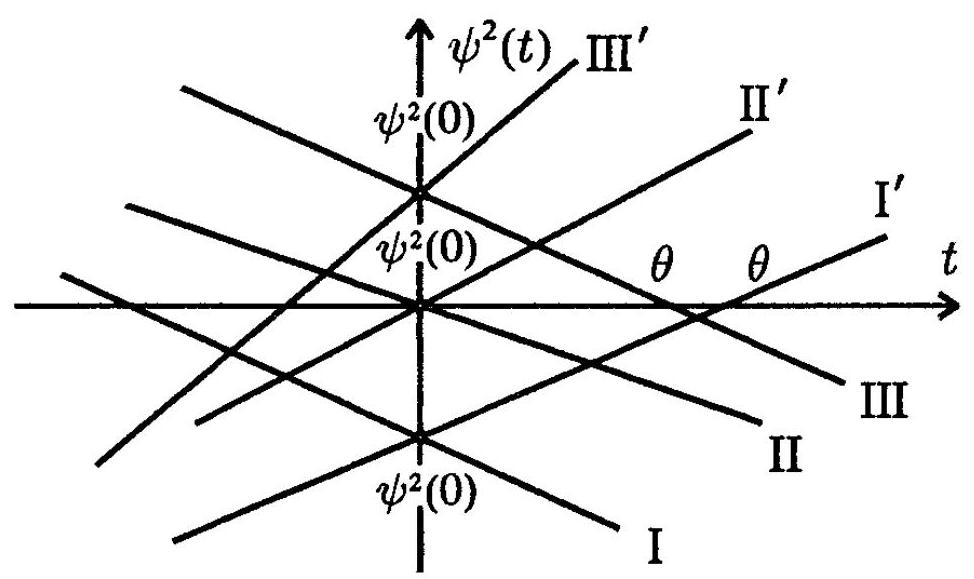
\includegraphics[max width=0.9\textwidth]{images/bo_d547okref24c73bgfch0_138_245_1540_974_579_0.jpg}
\end{center}
\hspace*{3em} 

Рис. 45

\begin{center}
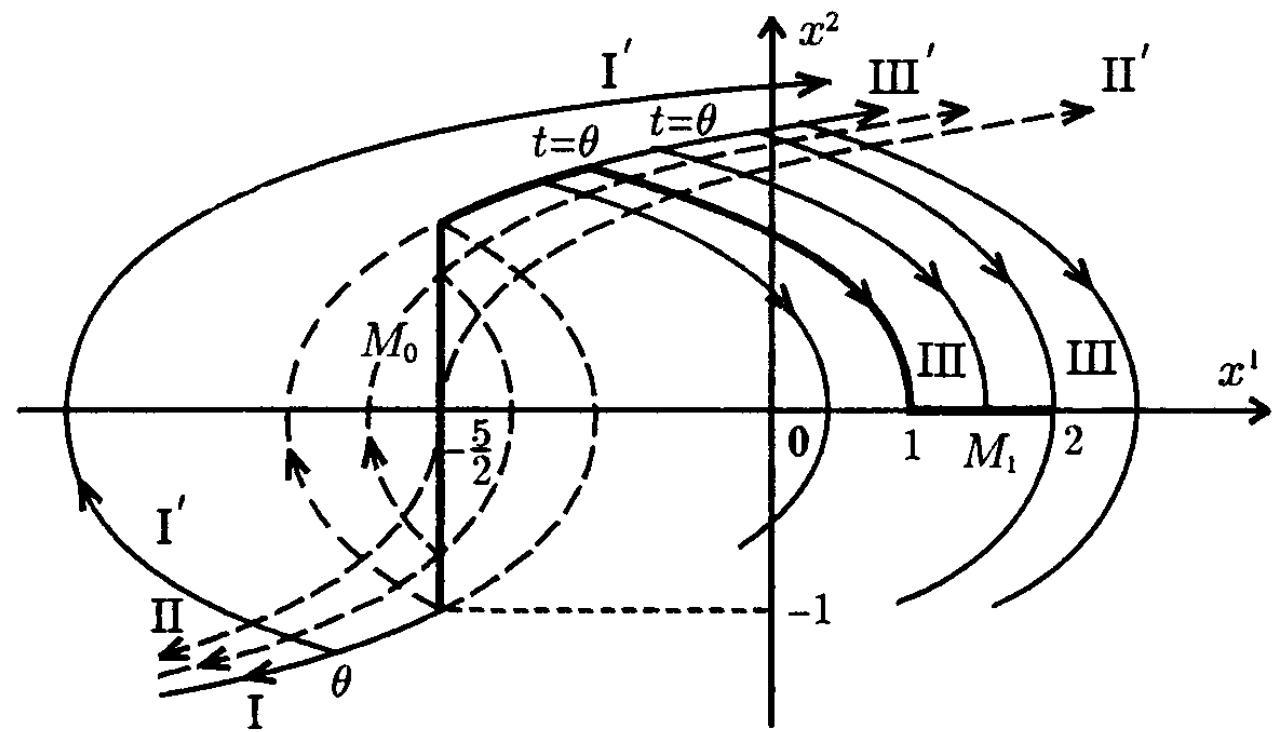
\includegraphics[max width=1.0\textwidth]{images/bo_d547okref24c73bgfch0_139_96_0_1283_732_0.jpg}
\end{center}
\hspace*{3em} 

Рис. 46

Случай 3. Если \({\psi }^{2}\left( 0\right)  > 0\) , то из условия трансверсальнос- ти на множестве \({M}_{0}\) следует, что начальная точка \(\mathbf{x}\left( 0\right)  = \left( {-\frac{5}{2}, + 1}\right)\) . Функция \({\psi }^{2}\left( t\right)\) в этом случае может быть положительной при всех \(t \geq  0\) , если \({\psi }^{1}\left( 0\right)  \leq  0\) (прямая III' на рис. 45), либо, начиная с некоторого момента времени \(\theta  > 0\) , стать отрицательной, если \({\psi }^{1}\left( 0\right)  > 0\) (прямая III на рис. 45). При этом момент \(\theta\) может быть сделан произвольным, так как он определяется из условия \(0 =  - {\psi }^{1}\left( 0\right) \theta  + {\psi }^{2}\left( 0\right)\) . Следовательно, согласно условию максимума (10.8) управление \({u}^{2}\left( t\right)\) имеет вид \({u}^{2}\left( t\right)  \equiv   + 1\) , или, начиная с момента времени \(\theta\) , переключится на \(-1\) . Если \({u}^{2}\left( t\right)  \equiv   + 1\) , то траектория \(\mathbf{x}\left( t\right)\) с начальным условием \(\mathbf{x}\left( 0\right)  = \left( {-\frac{5}{2}, + 1}\right)\) никогда не достигнет множества \({M}_{1}\) . Такая траектория также изображена на рис. 46 и обозначена цифрой III'. Если управление \({u}^{2}\left( t\right)\) вначале равно \(+1\) , а затем \(-1\) , то при некоторых \(\theta\) траектории такого вида достигнут множества \({M}_{1}\) . Эти траектории обозначены на рис. 46 цифрой III. Из рис. 46 видно, что таких траекторий много, и в каждую точку мно- жества \({M}_{1}\) попадет одна траектория данного вида. Проверим условие трансверсальности на множестве \({M}_{1}\) (10.10). Поскольку для всех траекторий данного вида \({\psi }^{1}\left( 0\right)  > 0\) , из соотношения (10.10) следует, что конечная точка траектории \(\mathbf{x}\left( t\right)\) определяет- ся условием \({x}^{1}\left( {t}_{1}\right)  = 1\) . Этому конечному условию удовлетворяет лишь одна траектория данного типа. На рис. 46 она изображена жирной линией.

Найдем эту единственную траекторию, удовлетворяющую принципу максимума. Точка \(\mathbf{x}\left( \theta \right)\) лежит на пересечении парабо- лы типа I, проходящей через точку \(\left( {-\frac{5}{2}, + 1}\right)\) , и параболы типа II, проходящей через точку \((1,0)\) . Найдем ее, исходя из этого условия. Парабола I задается уравнением \({x}^{1} = \frac{1}{2}{\left( {x}^{2}\right) }^{2} - 3\) , а па- рабола II — уравнением \({x}^{1} =  - \frac{1}{2}{\left( {x}^{2}\right) }^{2} + 1\) . Точка их пересечения \(\mathbf{x}\left( \theta \right)  = \left( {-1,2}\right)\) . Движение начинается из точки \(\mathbf{x}\left( 0\right)  = \left( {-\frac{5}{2}, + 1}\right)\) с управлением \({u}^{2}\left( t\right)  =  + 1\) . Из уравнения (10.11) найдем траекто- рию \(\mathbf{x}\left( t\right)\) с начальным условием \(\mathbf{x}\left( 0\right)  = \left( {-\frac{5}{2},1}\right)\) . Имеем решение

\[
{x}^{1}\left( t\right)  = \frac{1}{2}{\left( t + 1\right) }^{2} - 3,\;{x}^{2}\left( t\right)  = t + 1.
\]

По такой траектории будет двигаться точка до момента време- ни \(\theta\) , который определяется из условия попадания траектории \(\mathbf{x}\left( t\right)\) в точку \((-1,2)\) . Имеем \(2 = \theta  + 1\) , откуда \(\theta  = 1\) . Начиная с этого момента времени управление \({u}^{2}\left( t\right)\) равно \(-1\) . Дальнейшую траекторию найдем, решая уравнение (10.6) при \({u}^{2}\left( t\right)  =  - 1\) с начальным условием \(\mathbf{x}\left( 1\right)  = (-1,2)\) . Имеем соответственно решение

\[
{x}^{1}\left( t\right)  =  - \frac{{\left( t - 3\right) }^{2}}{2} + 1,\;{x}^{2}\left( t\right)  =  - \left( {t - 3}\right) .
\]

Момент времени \({t}_{1}\) определяется из условия попадания траек- тории в конечную точку \((1,0)\) . Получаем \({t}_{1} = 3\) .

Итак, мы установили, что единственное управление \(\mathbf{u}\left( t\right)\) удовлетворяет принципу максимума Понтрягина и переводит ракету из множества \({M}_{0}\) на множество \({M}_{1}\) на отрезке времени \(I = \left\lbrack  {0,3}\right\rbrack\) . По теореме существования оптимального управления в данной задаче оптимальное управление существует. По те- ореме о необходимых условиях оптимальности это управление должно удовлетворять принципу максимума. А так как мы на- шли единственное управление \(\mathbf{u}\left( t\right)\) , удовлетворяющее принципу максимума, то, следовательно, это управление \(\mathbf{u}\left( t\right)\) оптимально.

Пример 2. Найдем оптимальное управление, переводящее объект, описываемый системой уравнений

\[
\left\{  \begin{array}{l} {\dot{x}}^{1} = {x}^{2} \\  {\dot{x}}^{2} = {u}^{2},\;\left| {u}^{2}\right|  \leq  1 \end{array}\right. \tag{10.12}
\]

из начального множества \({M}_{0} = \{ \left( {-\frac{1}{2},1}\right) \}\) на конечное множество \({M}_{1} = \{ \left( {\frac{1}{2},1}\right) \}\) за наименьшее время.

Этот пример отличается от предыдущего только начальным и конечным множествами. Поэтому сопряженная система урав- нений имеет вид (10.7), а условие максимума задается соотноше- ниями (10.8). Для управления \({u}^{2}\left( t\right)\) ,удовлетворяющего условию максимума (10.8), возможны лишь четыре случая: управление \({u}^{2}\left( t\right)\) постоянно при всех t ≥ 0 и принимает значение +1 или -1; управление \({u}^{2}\left( t\right)\) переключается \(\mathrm{c} + 1\) на -1 или c -1 на +1 в некоторый момент времени 9 > 0 (см. рис. 42 и 45). Когда \({u}^{2}\left( t\right)  =  + 1\) ,движение происходит по параболам,изображенным на рис. 43, a когда \({u}^{2}\left( t\right)  =  - 1\) ,движение фазовой точки проис- ходит по параболам, изображенным на рис. 44.

Множества М0 и М1 в данном примере состоят из одной точки, следовательно, условия трансверсальности (10.4) и (10.5) выполняются автоматически с любой сопряженной функцией ψ(t). Таким образом, принцип максимума сводится к тому, что управление \({u}^{2}\left( t\right)\) имеет один из четырех описанных выше видов.

Найдем все управления, удовлетворяющие принципу макси- мума Понтрягина, используя схему, изображенную на рис. 40. Если управление \({u}^{2}\left( t\right)\) не имеет переключения, а равно +1 или -1при всех t ≥0,то такие траектории \(x\left( t\right)\) ,начинающиеся на множестве \({M}_{0}\) ,не попадают на множество \({M}_{1}\) . Они обозначены на Рис. 47 цифрами I и II, соответственно. Если управление \({u}^{2}\left( t\right)\) переключается с +1 на −1 в некоторый момент времени \(\theta\) , то одна из таких траекторий достигнет множества М1. Эти траектории обозначены на рис. 47 цифрой III. Если управление переключается с –1 на +1 в некоторый момент времени 0, то также одна из таких траекторий достигает конечного множест- ва \({M}_{1}\) . Эти траектории обозначены на рис. 47 цифрой IV.

Таким образом, принципу максимума Понтрягина удовле- творяют два различных управления. Зная фазовые траектории, т.е. параболы, изображенные на рис. 47, и используя систему уравнений (10.12), уже нетрудно найти два эти управления и

\begin{center}
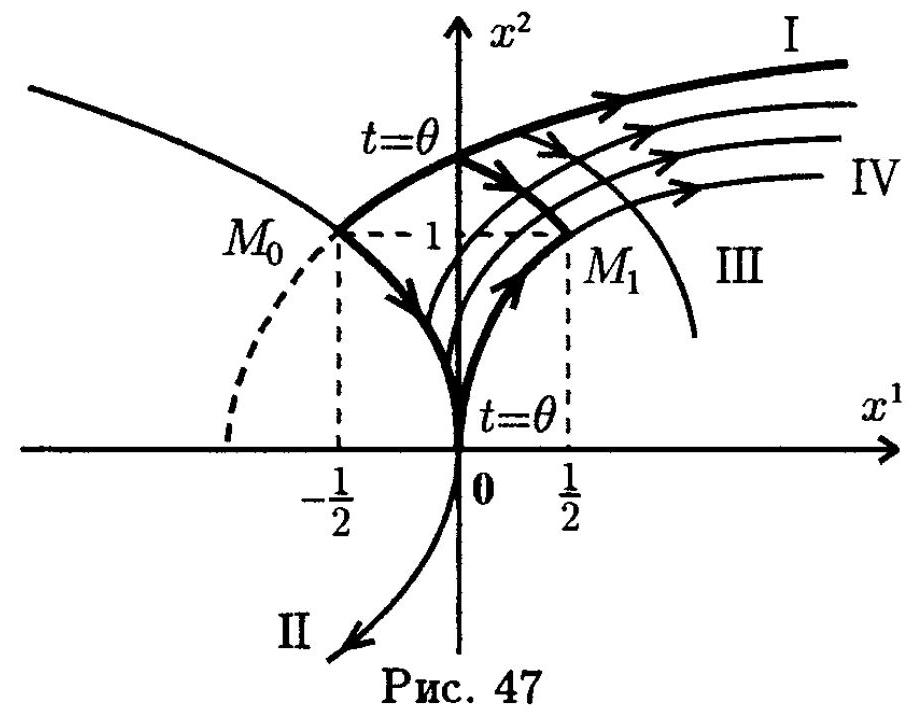
\includegraphics[max width=0.8\textwidth]{images/bo_d547okref24c73bgfch0_142_275_0_921_714_0.jpg}
\end{center}
\hspace*{3em} 

соответствующие решения х(t). Вычислим их таким же спосо- бом, как и в примере 1.

Первое управление имеет вид

\[
{u}^{2}\left( t\right)  = \left\{  \begin{array}{ll}  + 1, & \text{ если }0 \leq  t \leq  \sqrt{2} - 1, \\   - 1, & \text{ если }\sqrt{2} - 1 < t \leq  2\sqrt{2} - 2, \end{array}\right.
\]

и соответствующее решение

\[
\mathbf{x}\left( t\right)  = \left\{  \begin{array}{ll} \left( {\frac{1}{2}{t}^{2} + t - \frac{1}{2},t + 1}\right) , & \text{ если }0 \leq  t \leq  \sqrt{2} - 1, \\  \left( {-\frac{1}{2}{t}^{2} + \left( {2\sqrt{2} - 1}\right) t + 2\sqrt{2} - \frac{3}{2}, - t + 2\sqrt{2} - 1}\right) , & \\   & \text{ если }\sqrt{2} - 1 < t \leq  2\sqrt{2} - 2 \end{array}\right.
\]

осуществляет переход из начального множества \({M}_{0} = \{ \left( {-\frac{1}{2},1}\right) \}\) на конечное множество \({M}_{1} = \left\{  \left( {\frac{1}{2},1}\right) \right\}\) на отрезке времени \(\left\lbrack  {0,2\sqrt{2} - 2}\right\rbrack\) .

Второе управление имеет вид

\[
{u}^{2}\left( t\right)  = \left\{  \begin{array}{ll}  - 1, & \text{ если }0 \leq  t \leq  1, \\   + 1, & \text{ если }1 < t \leq  2, \end{array}\right.
\]

и соответствующее решение

\[
\mathbf{x}\left( t\right)  = \left\{  \begin{array}{ll} \left( {-\frac{1}{2}{t}^{2} + t - \frac{1}{2}, - t + 1}\right) , & \text{ если }0 \leq  t \leq  1, \\  \left( {\frac{1}{2}{t}^{2} - t + \frac{1}{2},t - 1}\right) , & \text{ если }1 < t \leq  2 \end{array}\right.
\]

осуществляет переход из \({M}_{0}\) на \({M}_{1}\) на отрезке времени \(\left\lbrack  {0,2}\right\rbrack\) .

Сравнивая время перехода из \({M}_{0}\) на \({M}_{1}\) при этих управле- ниях, \(0{,}82 \approx  2\sqrt{2} - 2 < 2\) , получаем, что первое управление оптимально, а второе — нет.

В примере 2 мы столкнулись с ситуацией, когда принципу максимума Понтрягина удовлетворяет несколько пар и(t), x(t). Это указывает на необходимость получения достаточных усло- вий оптимальности, с помощью которых можно было бы из всех управлений, удовлетворяющих принципу максимума, выбрать действительно оптимальное управление. Такие достаточные условия оптимальности будут выведены в следующей лекции.

Рассмотрим еще один пример, поясняющий геометрический смысл принципа максимума, вытекающий из леммы об эквива- лентной формулировке принципа максимума Понтрягина (см. лекцию 9).

Пример 3. Найдем оптимальное управление, переводящее объект, описываемый системой уравнений

\[
\left\{  \begin{array}{l} {\dot{x}}^{1} = {x}^{2} + {u}^{1} \\  {\dot{x}}^{2} =  - {x}^{1} + {u}^{2} \end{array}\right. \tag{10.13}
\]

c ограничением на управление \(u \in  U = {S}_{1}\left( 0\right)\) ,из начального множества \({M}_{0} = \{ 0\}\) на конечное множество

\[
{M}_{1} = \left\{  {\mathbf{x} \in  {E}^{2} : {x}^{1} = {2\pi },\left| {x}^{2}\right|  \leq  1}\right\} \tag{10.14}
\]

за наименьшее время.

Для решения этой задачи применим принцип максимума. Cопряженная система уравнений (10.2) принимает вид

\[
\left\{  \begin{array}{l} {\dot{\psi }}^{1} = {\psi }^{2} \\  {\dot{\psi }}^{2} =  - {\psi }^{1} \end{array}\right.
\]

Пусть \({t}_{0} = 0\) . Найдем решение фи() этой системы с произволь- ным начальным условием

\[
\psi \left( 0\right)  = \left( {\cos \alpha ,\sin \alpha }\right)  \in  S. \tag{10.15}
\]

Для матрицы \(A = \left( \begin{array}{cc} 0 & 1 \\   - 1 & 0 \end{array}\right)\) экспоненциал \({e}^{tA}\) имеет вид

\[
{e}^{tA} = \left( \begin{array}{cc} \cos t & \sin t \\   - \sin t & \cos t \end{array}\right) \tag{10.16}
\]

(см. пример 2 из лекции 6). Таким образом, решение ф(н) зада- ется соотнощением (см. формулу \(\left( {9.10}\right)\) излекции9)

\[
\psi \left( t\right)  = {e}^{-t{A}^{ * }}\psi \left( 0\right)  = {e}^{tA}\psi \left( 0\right)  =
\]

\[
= \left( \begin{array}{cc} \cos t & \sin t \\   - \sin t & \cos t \end{array}\right) \left( \begin{array}{c} \cos \alpha \\  \sin \alpha \end{array}\right)  = \left( \begin{array}{c} \cos \left( {\alpha  - t}\right) \\  \sin \left( {\alpha  - t}\right) \end{array}\right) . \tag{10.17}
\]

Условие максимума (10.3) приобретает вид

\[
\langle \mathbf{u}\left( t\right) ,\mathbf{\psi }\left( t\right) \rangle  = c\left( {U,\mathbf{\psi }\left( t\right) }\right)  = \parallel \mathbf{\psi }\left( t\right) \parallel .
\]

Поскольку ||\#(t)|| = 1, из этого условия однозначно определяет- ся управление

\[
\mathbf{u}\left( t\right)  = \psi \left( t\right)  = \left( {\cos \left( {\alpha  - t}\right) ,\sin \left( {\alpha  - t}\right) }\right) . \tag{10.18}
\]

Условие трансверсальности на множестве Мо (10.4) выполня- ется автоматически, так как множество \({M}_{0}\) состоит из одной точки \({\mathbf{x}}_{0} = 0\) , a условие трансверсальности на множестве М1 (10.5) в силу формулы (10.14) имеет вид

\[
- {x}^{1}\left( {t}_{1}\right) {\psi }^{1}\left( {t}_{1}\right)  - {x}^{2}\left( {t}_{1}\right) {\psi }^{2}\left( {t}_{1}\right)  =  - {2\pi }{\psi }^{1}\left( {t}_{1}\right)  + \left| {{\psi }^{2}\left( {t}_{1}\right) }\right| .
\]

Следовательно, выполняются соотношения

\[
{x}^{2}\left( {t}_{1}\right)  =  + 1\text{ , ecли }{\psi }^{2}\left( {t}_{1}\right)  < 0,
\]

\[
{x}^{2}\left( {t}_{1}\right)  =  - 1\text{ ,если }{\psi }^{2}\left( {t}_{1}\right)  > 0, \tag{10.19}
\]

\[
- 1 \leq  {x}^{2}\left( {t}_{1}\right)  \leq  1,\;\text{ если }\;{\psi }^{2}\left( {t}_{1}\right)  = 0.
\]

Найдемвсепары \(\mathbf{u}\left( t\right) ,\mathbf{x}\left( t\right)\) ,удовлетворяющие принципу мак- симума Понтрягина,в соответствии со схемой,приведенной на PHC. 40.

Пля этого найдем рещения системы уравнений (10.13) с управлениями \(\mathbf{u}\left( t\right)\) ,заданными формулой \(\left( {10.18}\right)\) ,и начальным условием х \(\left( 0\right)  = {0.3}\) апишем рещение к(т) поформуле Кощи (cm. лекцию 6)

\[
\mathbf{x}\left( t\right)  = {e}^{\left( {t - {t}_{0}}\right) A}\mathbf{x}\left( {t}_{0}\right)  + {\int }_{{t}_{0}}^{t}{e}^{\left( {t - s}\right) A}\mathbf{u}\left( s\right) {ds}.
\]

Подставляя в эту формулу конкретные значения и учитывая выражение (10.16), получаем решение

\[
\mathbf{x}\left( t\right)  = \left( {t\cos \left( {\alpha  - t}\right) ,t\sin \left( {\alpha  - t}\right) }\right) . \tag{10.20}
\]

Таким образом, выражение (10.20) дает все решения, удовле- творяющие условию максимума (10.3) и условию трансверсаль- ности на множестве \({M}_{0}\) . При этом решения х(t) зависят от на- чального вектора ф(О) сопряженной функции ψ(t) (см. формулу (10.15)).

\begin{center}
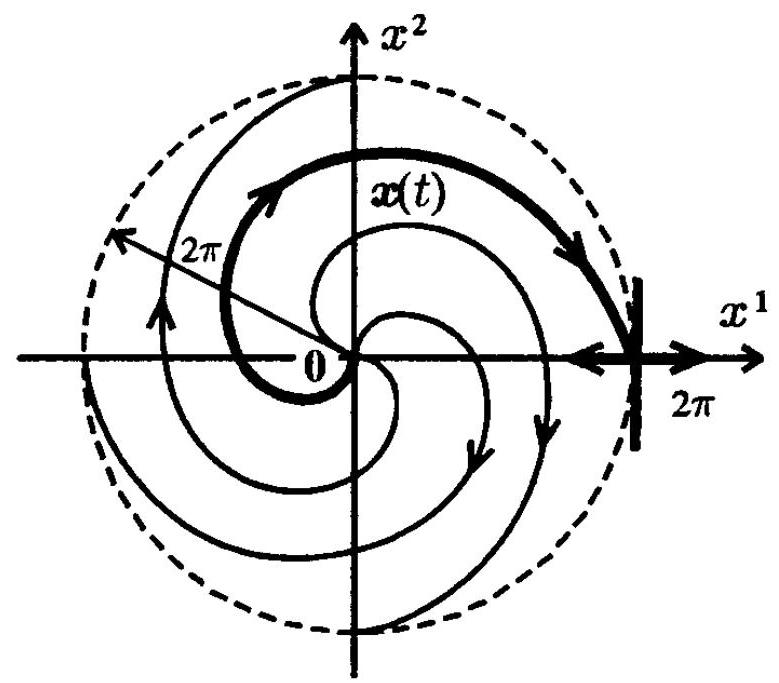
\includegraphics[max width=0.7\textwidth]{images/bo_d547okref24c73bgfch0_145_341_0_779_683_0.jpg}
\end{center}
\hspace*{3em} 

Рис. 48

Tpaexтории \(x\left( t\right)\) ,заданные выражением (10.20), oбразуют в фазовой плоскости \(x = \left( {{x}^{1},{x}^{2}}\right)\) семейство спиралей (рис. 48). Поскольку || \(\mathbf{x}\left( t\right)\) || \(= t\) , \(\mathbf{B}\) момент времени к все решения х \(\mathbf{x}\left( t\right)\) находятся на окружности радиуса и с центром в точке х = 0. Понятно, что эти решения впервые достигнут множества М1 в момент времени \({t}_{1} = {2\pi }\) . Это будет траектория \(x\left( t\right)\) ,изобра- женная на рис. 48 жирной линией, она соответствует значению параметра \(\alpha  = 0\) ,т.е.

\[
x\left( t\right)  = \left( {t\cos t, - t\sin t}\right) ,\;0 \leq  t \leq  {2\pi }.
\]

Остается только проверить условие трансверсальности на мно- жестве \({M}_{1}\left( {10.19}\right)\) . Поскольку при \(\alpha  = 0\) из формулы (10.17) получаем сопряженную функцию

\[
\psi \left( t\right)  = \left( {\cos t, - \sin t}\right) \tag{10.21}
\]

то \({\psi }^{2}\left( {2\pi }\right)  = 0\) ,и соотношение (10.19) выполняется.

Таким образом, единственная пара

\[
\mathbf{u}\left( t\right)  = \left( {\cos t, - \sin t}\right) ,\;\mathbf{x}\left( t\right)  = \left( {t\cos t, - t\sin t}\right)
\]

осуществляет переход из множества \({M}_{0}\) на множество \({M}_{1}\) на отрезке времени \(\left\lbrack  {0,{2\pi }}\right\rbrack\) и удовлетворяет принципу максимума Понтрягина. Следовательно, эта пара и(t), х(t) оптимальна.

Продемонстрируем на этом примере геометрический смысл принципа максимума. Для этого вычислим множество дости- жимости \(X\left( t\right)\) и множество управляемости \(Y\left( t\right)\) . Они задаются формулами (см. лекцию 7)

\[
X\left( t\right)  = {e}^{\left( {t - {t}_{0}}\right) A}{M}_{0} + {\int }_{{t}_{0}}^{t}{e}^{\left( {t - s}\right) A}{Uds}
\]

\[
Y\left( t\right)  = {e}^{\left( {t - {t}_{1}}\right) A}{M}_{1} + {\int }_{t}^{{t}_{1}}{e}^{\left( {t - s}\right) A}\left\lbrack  {-U}\right\rbrack  {ds}.
\]

Подставляя в эти формулы конкретные значения и учитывая, что матрица (10.16) осуществляет поворот на угол t по часовой стрелке, получим выражения

\[
X\left( t\right)  = {S}_{t}\left( 0\right) ,\;Y\left( t\right)  = \left( \begin{array}{cc} \cos t & \sin t \\   - \sin t & \cos t \end{array}\right) {M}_{1} + {S}_{{2\pi } - t}\left( 0\right) .
\]

Таким образом, множество достижимости \(X\left( t\right)\) есть круг радиуса t с центром в начале координат, а множество управ- ляемости \(Y\left( t\right)\) — сумма отрезка \({M}_{1}\) ,повернутого на угол t по часовой стрелке, и круга радиуса 2π - t с центром в начале координат.

На рис. 49 — 53 показано в динамике изменение множеств достижимости \(X\left( t\right)\) и управляемости \(Y\left( t\right)\) . При этом видно,что для всех моментов времени к ∈ [0,2π] сопряженный вектор \(\psi \left( t\right)\) , задаваемый формулой (10.21), является опорным вектором к множеству достижимости \(X\left( t\right)\) в точке x(t). Аналогично вектор \(- \psi \left( t\right)\) является опорным вектором к множеству управляемости \(Y\left( t\right)\) в точке \(x\left( t\right)\) . Гиперплоскость

\[
{\Gamma }_{\psi \left( t\right) } = \left\{  {\mathbf{x} \in  {E}^{n} : \langle \mathbf{x} - \mathbf{x}\left( t\right) ,\psi \left( t\right) \rangle  = 0}\right\}
\]

разделяет множества \(X\left( t\right)\) и \(Y\left( t\right)\) . Таков геометрический смысл принципа максимума Понтрягина.

\begin{center}
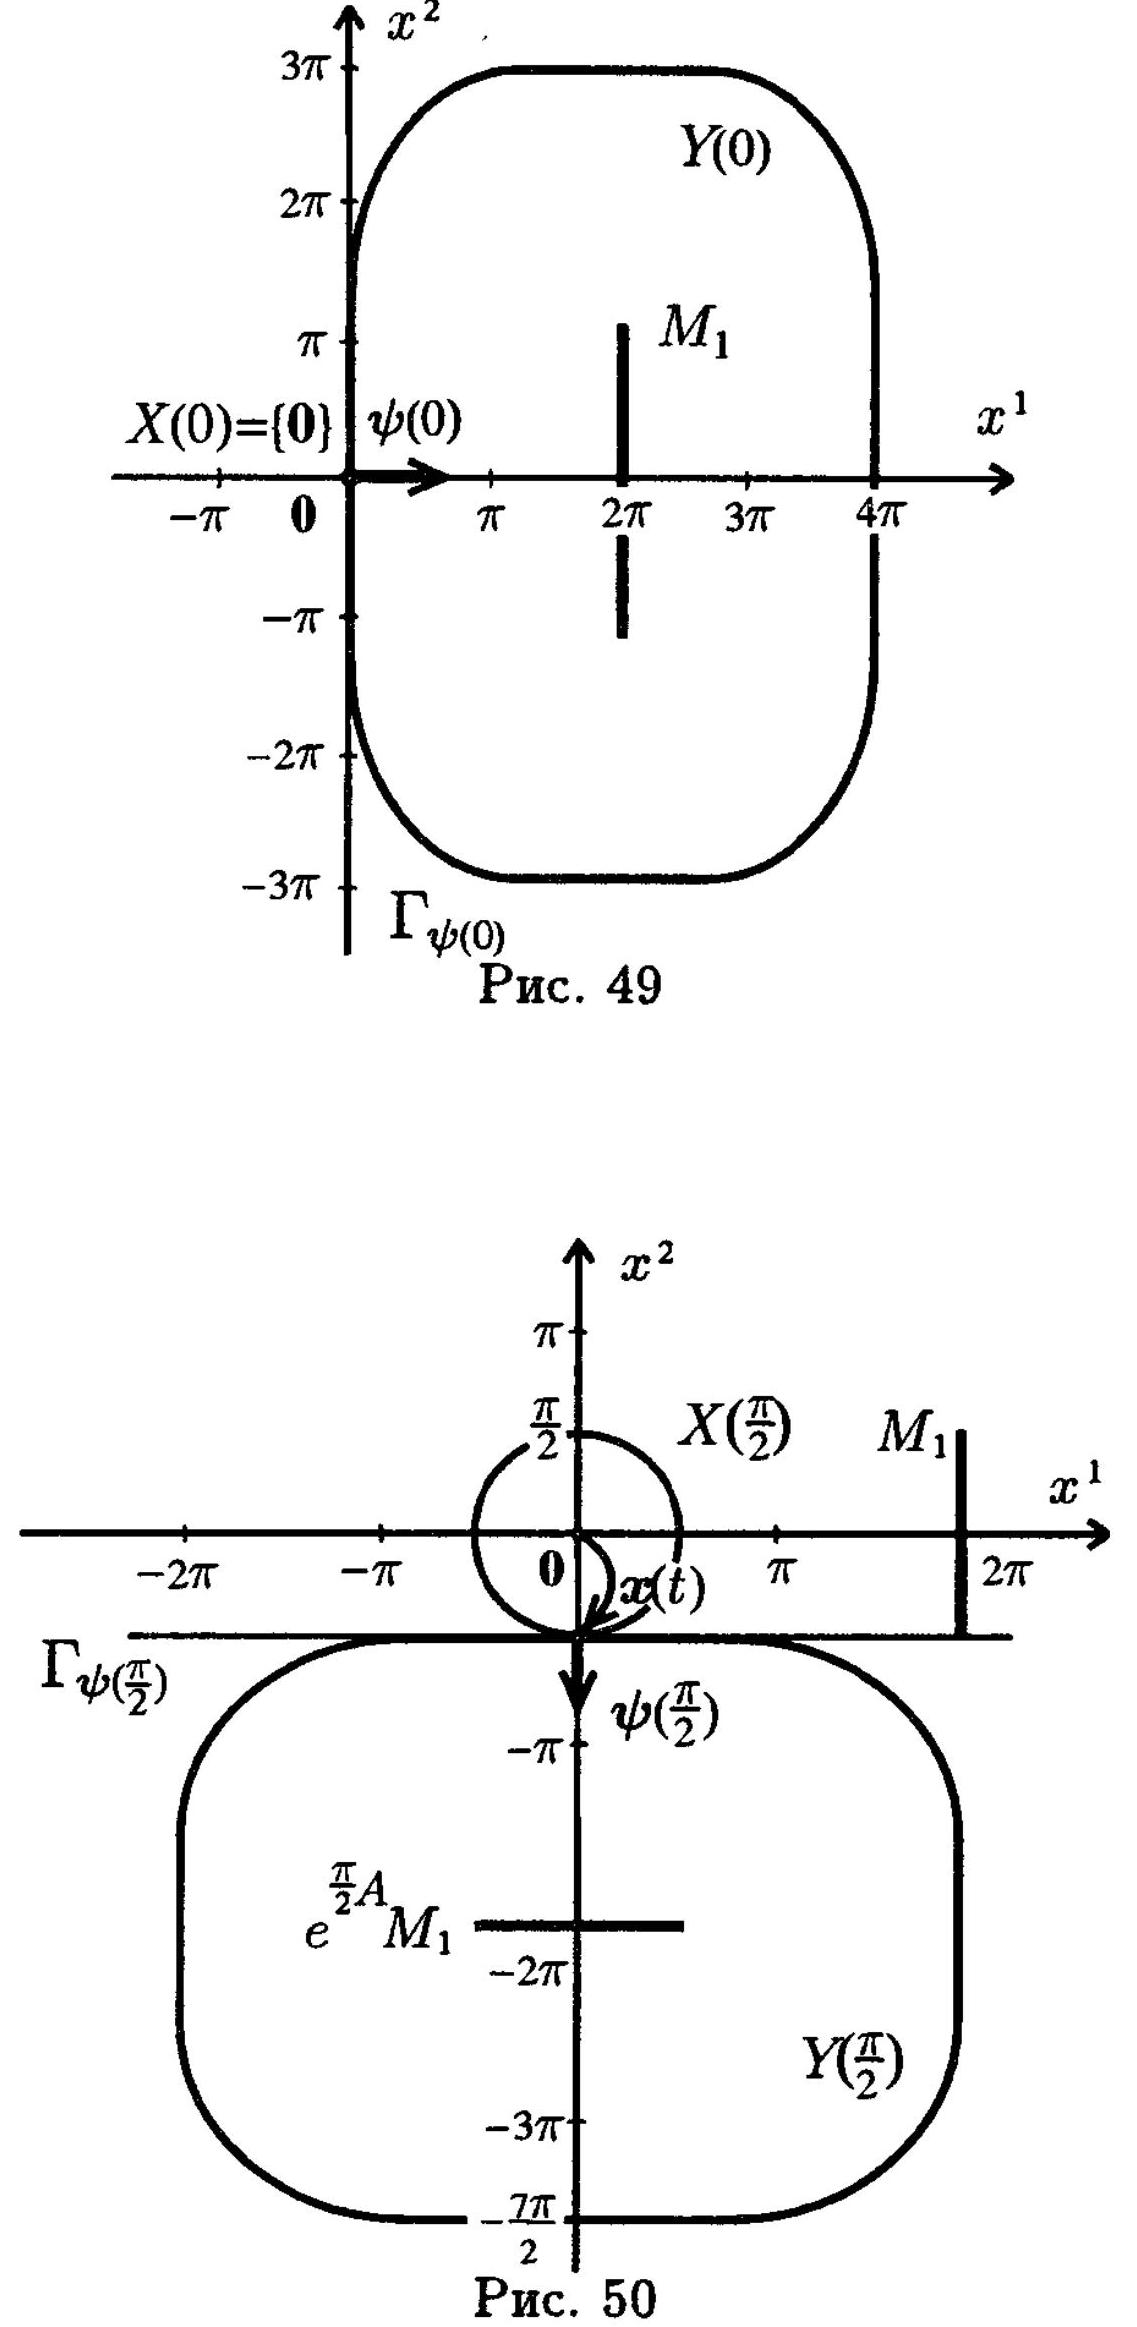
\includegraphics[max width=1.0\textwidth]{images/bo_d547okref24c73bgfch0_147_6_11_1137_2327_0.jpg}
\end{center}
\hspace*{3em} 

\begin{center}
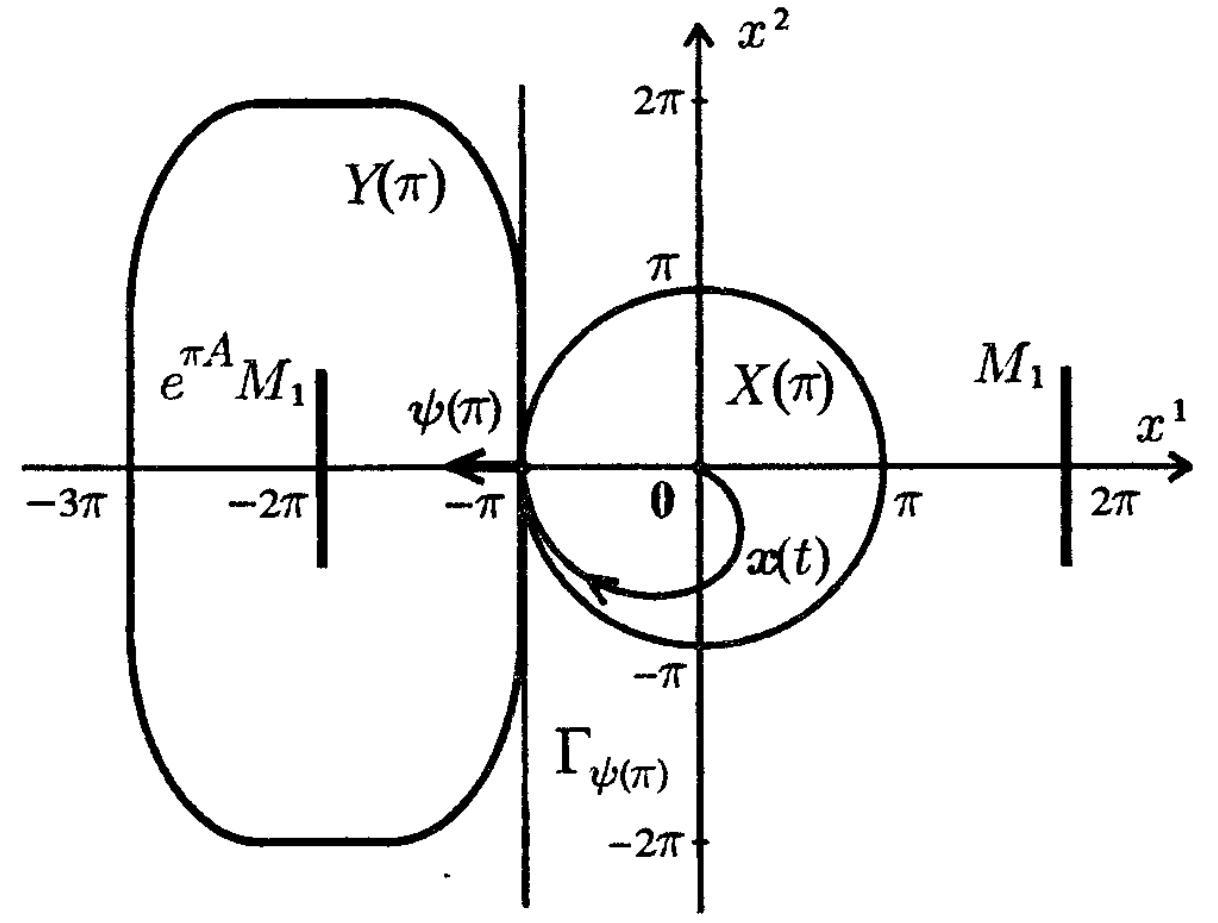
\includegraphics[max width=1.0\textwidth]{images/bo_d547okref24c73bgfch0_148_8_0_1218_923_0.jpg}
\end{center}
\hspace*{3em} 

Рис. 51

\begin{center}
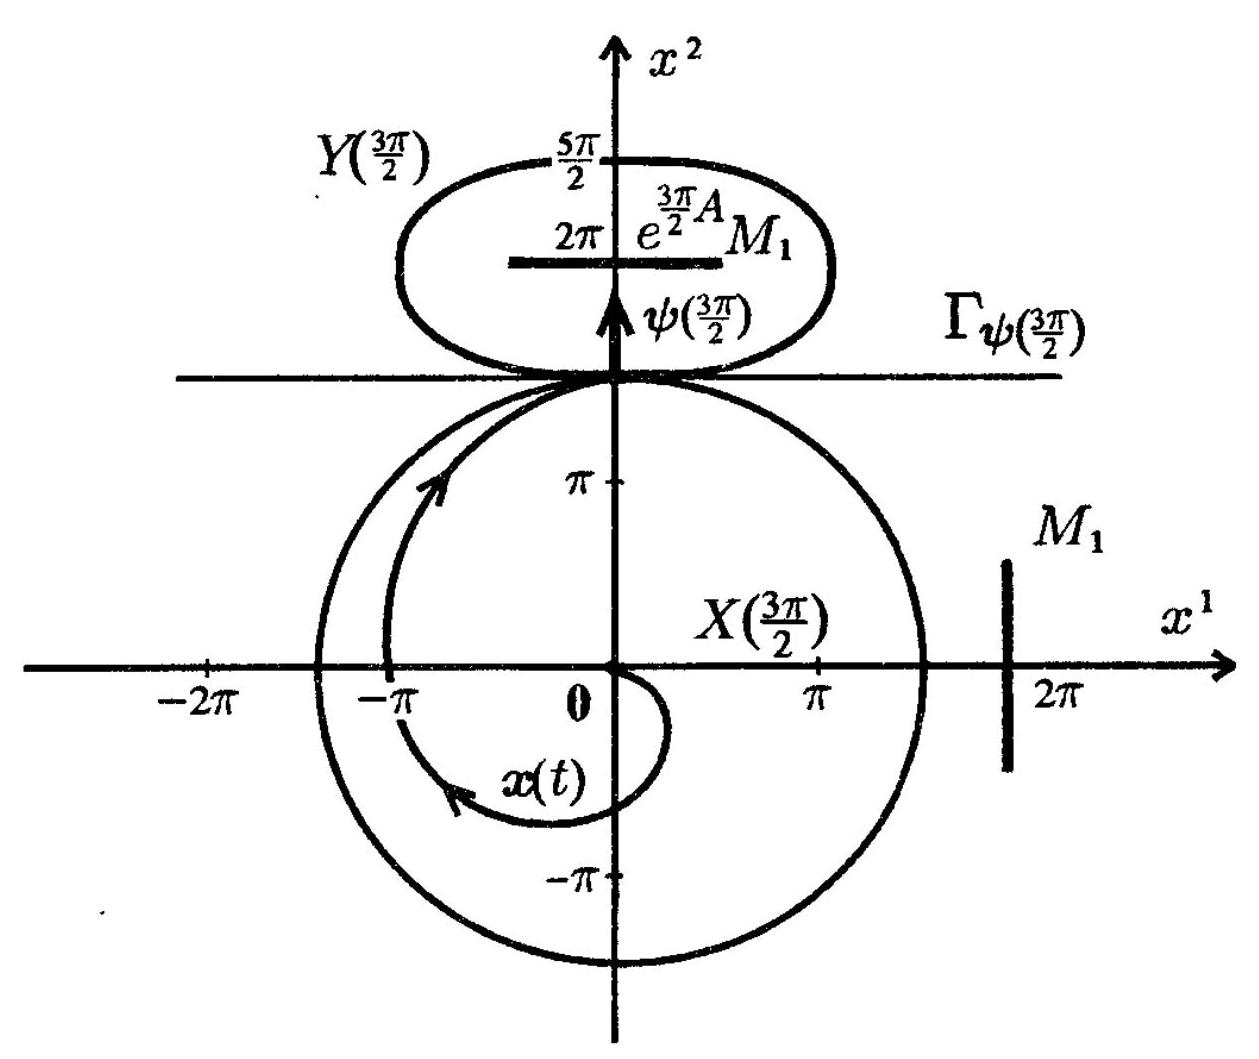
\includegraphics[max width=1.0\textwidth]{images/bo_d547okref24c73bgfch0_148_11_1131_1259_1059_0.jpg}
\end{center}
\hspace*{3em} 

Рис. 52

\begin{center}
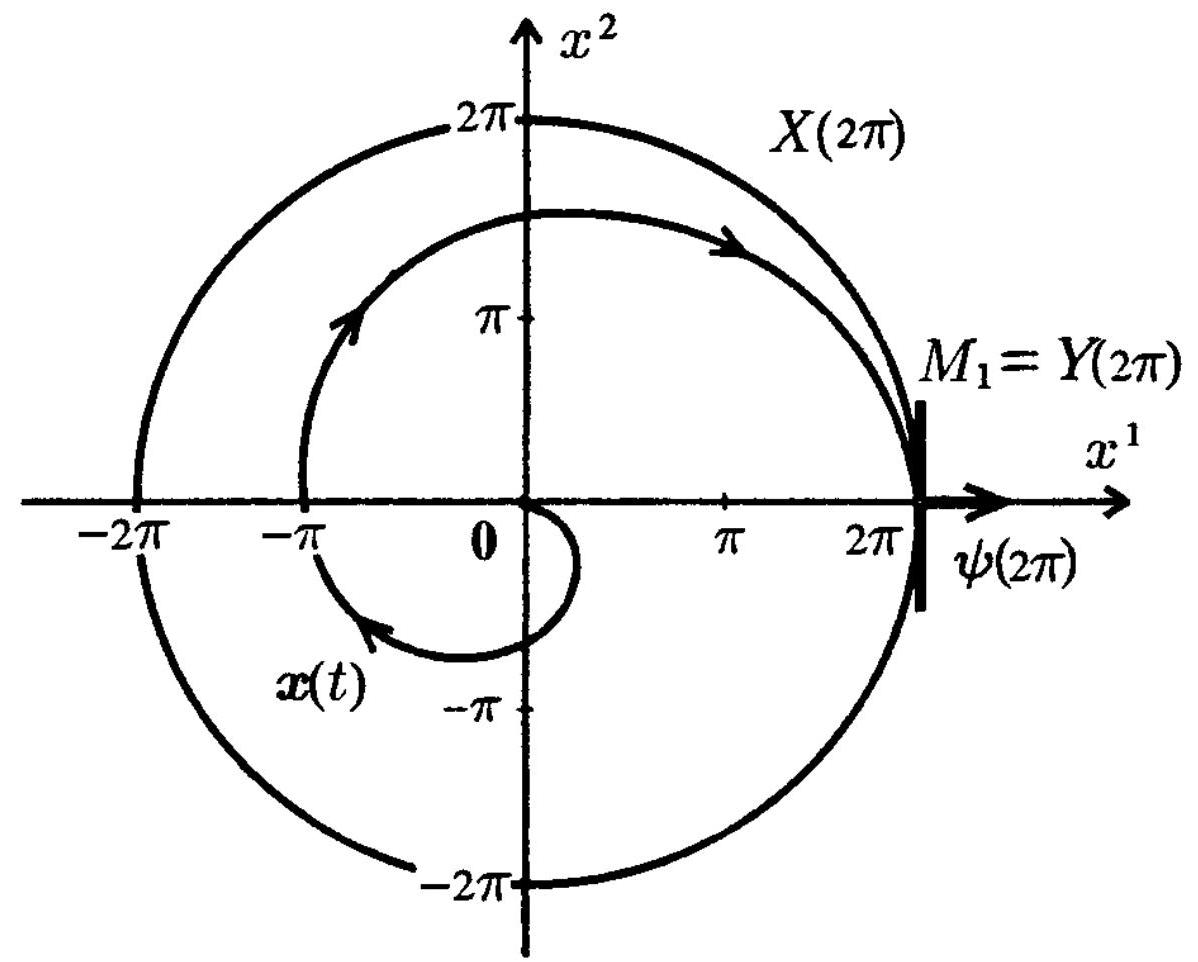
\includegraphics[max width=0.9\textwidth]{images/bo_d547okref24c73bgfch0_149_319_0_1198_962_0.jpg}
\end{center}
\hspace*{3em} 

Pис. 53

\section*{10.2. Задачи}

1. Найдите оптимальное управление, переводящее объект, описываемый системой уравнений

\[
\left\{  \begin{array}{l} {\dot{x}}^{1} = {x}^{2}, \\  {\dot{x}}^{2} = v,\;\left| v\right|  \leq  1, \end{array}\right. \tag{10.22}
\]

из начального множества

\[
{M}_{0} = \left\{  {\mathbf{x} \in  {E}^{2} :  - 5 \leq  {x}^{1} \leq   - 4,{x}^{2} = 0}\right\}
\]

на конечное множество \({M}_{1} = \{ \mathbf{0}\}\) за наименьшее время.

2. Найдите оптимальное управление, переводящее объект, описываемый системой уравнений (10.22) из начального мно- жества \({M}_{0} = \{ 0\}\) на конечное множество

\[
{M}_{1} = \left\{  {\mathbf{x} \in  {E}^{2} : {x}^{1} = 5,\left| {x}^{2}\right|  \leq  2}\right\}
\]

3a HaMMehbluee BPEAA.

\section*{ЛЕКЦИЯ 11}

\begin{itemize}\relax
\item\relax Усиленные условия трансверсальности на множес- твах \({M}_{0}\) и \({M}_{1}\) .
\end{itemize}

\begin{itemize}\relax
\item\relax Теорема о достаточных условиях оптимальности.
\end{itemize}

\section*{11.1. Достаточные условия оптимальности}

Займемся теперь достаточными условиями оптимальности в линейной задаче быстродействия, которая заключается в нахож- дении допустимого управления и(t) ∈ U, переводящего объект, описываемый уравнением

\[
\dot{\mathbf{x}} = A\mathbf{x} + \mathbf{u}, \tag{11.1}
\]

из начального множества \({M}_{0}\) на конечное множество \({M}_{1}\) за наименьшее время. Достаточные условия оптимальности будут даны также в форме принципа максимума Понтрягина. По опре- делению пара \(\mathbf{u}\left( t\right) ,\mathbf{x}\left( t\right)\) удовлетворяет принципу максимума на отрезке времени \(I = \left\lbrack  {{t}_{0},{t}_{1}}\right\rbrack\) , если существует решение \(\psi \left( t\right)\) вспо- могательной сопряженной системы

\[
\dot{\psi } =  - {A}^{ * }\psi \tag{11.2}
\]

c начальным условием \(\mathbf{\psi }\left( {t}_{0}\right)  \in  S\) такое, что выполнены следую- щие три условия:

1) условие максимума

\[
\langle \mathbf{u}\left( t\right) ,\mathbf{\psi }\left( t\right) \rangle  = c\left( {U,\mathbf{\psi }\left( t\right) }\right) \tag{11.3}
\]

для почти всех t ∈ I;

2) условие трансверсальности на множестве Мо

\[
\left\langle  {\mathbf{x}\left( {t}_{0}\right) ,\mathbf{\psi }\left( {t}_{0}\right) }\right\rangle   = \mathrm{c}\left( {{M}_{0},\mathbf{\psi }\left( {t}_{0}\right) }\right) ; \tag{11.4}
\]

3) условие трансверсальности на множестве М1

\[
\left\langle  {\mathbf{x}\left( {t}_{1}\right) , - \psi \left( {t}_{1}\right) }\right\rangle   = c\left( {{M}_{1}, - \psi \left( {t}_{1}\right) }\right) . \tag{11.5}
\]

Оказывается, для то- го чтобы пара \(\mathbf{u}\left( t\right) ,\mathbf{x}\left( t\right)\) , удовлетворяющая принци- пу максимума Понтряги- на на отрезке времени \(I = \left\lbrack  {{t}_{0},{t}_{1}}\right\rbrack\) , была оптималь- ной, достаточно, чтобы она удовлетворяла еще одному из двух дополнительных условий. Эти условия назы- ваются усиленными усло- виями трансверсальности на множествах \({M}_{0}\) и \({M}_{1}\) со- ответственно.

\begin{center}
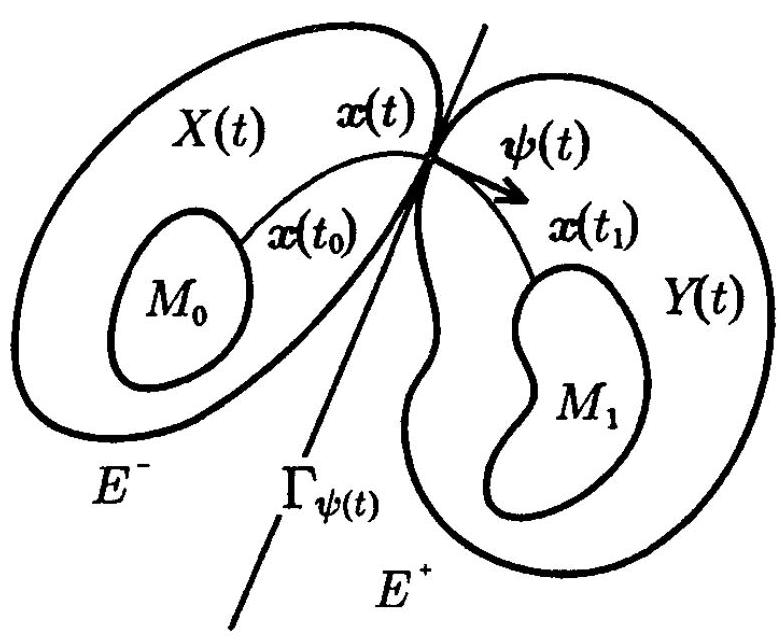
\includegraphics[max width=0.7\textwidth]{images/bo_d547okref24c73bgfch0_151_7_12_781_640_0.jpg}
\end{center}
\hspace*{3em} 

Рис. 54

Определение. Пусть \(\mathbf{x}\left( t\right)\) — траектория управляемой систе- мы (11.1) на отрезке времени \(I = \left\lbrack  {{t}_{0},{t}_{1}}\right\rbrack\) . Пусть далее \(\psi \left( t\right)\) — некоторое решение сопряженной системы (11.2). Бу- дем говорить, что решение \(\mathbf{x}\left( t\right)\) удовлетворяет усиленному условию трансверсальности на множестве \({M}_{0}\) с функцией \(\psi \left( t\right)\) на отрезке времени \(I\) , если для всех моментов времени \({t}_{0} < t \leq  {t}_{1}\) выполняется строгое неравенство

\[
\langle \mathbf{x}\left( t\right) ,\psi \left( t\right) \rangle  > c\left( {{M}_{0},\psi \left( t\right) }\right) . \tag{11.6}
\]

Далее, решение \(\mathbf{x}\left( t\right)\) удовлетворяет усиленному условию транс- версальности на множестве \({M}_{1}\) с функцией \(\psi \left( t\right)\) на отрезке времени \(I\) , если для всех моментов времени \({t}_{0} \leq  t < {t}_{1}\) выпол- няется строгое неравенство

\[
\langle \mathbf{x}\left( t\right) , - \psi \left( t\right) \rangle  > c\left( {{M}_{1}, - \psi \left( t\right) }\right) . \tag{11.7}
\]

Выясним геометрический смысл усиленных условий транс- версальности. Проведем через точку х(t) гиперплоскость \({\Gamma }_{\psi \left( t\right) }\) c вектором нормали ψ(t) (рис. 54). Гиперплоскость Гифи разде- ляет все пространство \({E}^{n}\) на два замкнутых полупространства: \({E}^{ + } -\) положительное относительно вектора ψ(t) полупростран- ство и Ег — отрицательное. Как мы уже знаем, эта гиперплос- кость разделяет множества достижимости \(X\left( t\right)\) и управляемос- ти \(Y\left( t\right)\) при всех и с хем пара и и(t), х(t) удовлетворяет принципу максимума на отрезке времени \(I = \left\lbrack  {{t}_{0},{t}_{1}}\right\rbrack\) c сопряжен- ной функцией \(\psi \left( t\right)\) .

Таким образом, множество достижимости \(X\left( t\right)\) принадле- жит полупространству \({E}^{ - }\) , a множество управляемости — по- лупространству E+. Усиленное условие трансверсальности на множестве \({M}_{0}\) ,т.е. неравенство (11.6), oзначает,что при всех \(t \leq  {t}_{0} < {t}_{1}\) множество \({M}_{0}\) лежит строго внутри отрицатель- ного полупространства E-. Аналогичным образом усиленное условие трансверсальности на множестве М1, т.е. неравенство (11.7), oзначает,что при всех t ≤ \({t}_{0} < {t}_{1}\) множество \({M}_{1}\) ле- жит строго внутри положительного полупространства E+ (см. puc. 54).

Термин "усиленное условие трансверсальности" на множес- тве Мо (11.6) подразумевает, что это условие сильнее обычного условия трансверсальности (11.4) на множестве М0. В дейст- вительности так оно и есть, и из неравенства (11.6) следует неравенство (11.4). В самом деле, пусть неравенство (11.6) вы- полняется при всех бо < t ≤ t, . Поскольку в неравенстве (11.6) слева и справа стоят непрерывные функции (см. следствие свой- ства 13 опорных функций, лекция 3), то, переходя к пределу при \(t \rightarrow  {t}_{0}\) ,получим неравенство

\[
\left\langle  {\mathbf{x}\left( t\right) ,\psi \left( {t}_{0}\right) }\right\rangle   \geq  c\left( {{M}_{0},\psi \left( {t}_{0}\right) }\right) .
\]

Tak как \(\mathbf{x}\left( {t}_{0}\right)  \in  {M}_{0}\) , то по свойствам опорных функций имеем неравенство

\[
\left\langle  {\mathbf{x}\left( {t}_{0}\right) ,\mathbf{\psi }\left( {t}_{0}\right) }\right\rangle   \leq  c\left( {{M}_{0},\mathbf{\psi }\left( {t}_{0}\right) }\right) .
\]

Из этих двух неравенств следует равенство (11.4).

Аналогичным образом из усиленного условия трансверсаль- ности на множестве М1 (11.7) следует обычное условие транс- версальности на множестве М1 (11.5).

Первая теорема о достаточных условиях оптималь- ности. Пусть и (t) ∈ U — некоторое допустимое управление, \(\mathbf{x}\left( t\right)  -\) coomвemcтвующее решение уравнения (11.1), nepеводя- щее объект из множества М0 на множество М1 на отрезке времени \(I = \left\lbrack  {{t}_{0},{t}_{1}}\right\rbrack\) . Предположим, что пара и(t), x(t) удов- летворяет принципу максимума Понтрягина на отрезке вре- мени I, а ψ(t) — соответствующая сопряженная функция. Далее, предположим, что решение х(t) с этой функцией ф(t) удовлетворяет на отрезке времени I одному из усиленных ус- ловий трансверсальности: либо на множестве Мо (11.6), либо на множестве М1 (11.7). Тогда управление и(t) оптимально.

Доказательство. Пусть v(t) ∈ U — произвольное допус- тимое управление на отрезке времени

\[
{I}^{\prime } = \left\lbrack  {{t}_{0}^{\prime },{t}_{1}^{\prime }}\right\rbrack   \subset  \left\lbrack  {{t}_{0},{t}_{1}}\right\rbrack   = I,
\]

а \(\mathbf{y}\left( t\right)\) — соответствующее решение уравнения (11.1). Рассмот- рим скалярную функцию

\[
\xi \left( t\right)  = \langle \mathbf{y}\left( t\right)  - \mathbf{x}\left( t\right) ,\psi \left( t\right) \rangle . \tag{11.8}
\]

Покажем, что для почти всех t ∈ I’ выполняется неравенство

\[
\dot{\xi }\left( t\right)  \leq  0\text{ . } \tag{11.9}
\]

Действительно, так как функции \(x\left( t\right)\) и \(y\left( t\right)\) являются ре- шениями уравнения (11.1) с управлениями и(t) и v(t) соответ- ственно, а ψ(t) — решение уравнения (11.2), то для почти всех \(t \in  {I}^{\prime }\) имеем соотношения

\[
\dot{\xi }\left( t\right)  = \langle \dot{\mathbf{y}}\left( t\right) ,\mathbf{\psi }\left( t\right) \rangle  - \langle \dot{\mathbf{x}}\left( t\right) ,\mathbf{\psi }\left( t\right) \rangle  + \langle \mathbf{y}\left( t\right) ,\dot{\mathbf{\psi }}\left( t\right) \rangle  - \langle \mathbf{x}\left( t\right) ,\dot{\mathbf{\psi }}\left( t\right) \rangle  =
\]

\[
= \langle A\mathbf{y}\left( t\right) ,\mathbf{\psi }\left( t\right) \rangle  + \langle \mathbf{v}\left( t\right) ,\mathbf{\psi }\left( t\right) \rangle  - \langle A\mathbf{x}\left( t\right) ,\mathbf{\psi }\left( t\right) \rangle  - \langle \mathbf{u}\left( t\right) ,\mathbf{\psi }\left( t\right) \rangle  +
\]

\[
+ \langle \mathbf{y}\left( t\right) , - {A}^{ * }\mathbf{\psi }\left( t\right) \rangle  - \langle \mathbf{x}\left( t\right) , - {A}^{ * }\mathbf{\psi }\left( t\right) \rangle  = \langle \mathbf{v}\left( t\right) ,\mathbf{\psi }\left( t\right) \rangle  - \langle \mathbf{u}\left( t\right) ,\mathbf{\psi }\left( t\right) \rangle .
\]

Далее, так как управление и(t) удовлетворяет условию мак- симума (11.3) для почти всех t ∈ I, получаем равенство

\[
\dot{\xi }\left( t\right)  = \langle v\left( t\right) ,\psi \left( t\right) \rangle  - \mathrm{c}\left( {U\left( t\right) ,\psi \left( t\right) }\right) .
\]

Поскольку управление v(t) допустимо, т.е. v(t) ∈ U, то согласно следствию из свойства 6 опорных функций имеем неравенство \(\dot{\xi }\left( t\right)  \leq  0\) для почти всех t ∈ I’. Таким образом, неравенство (11.9) доказано.

Теперь докажем, что управление и(t) оптимально на отрезке времени \(\left\lbrack  {{t}_{0},{t}_{1}}\right\rbrack\) в смысле быстродействия. Предположим против- ное, т.е. пусть существует такое допустимое управление v(t), что соответствующее решение уравнения (11.1) осуществляет переход из множества \({M}_{0}\) на множество М1 на отрезке времени \(\left\lbrack  {{t}_{0},{t}_{1} - \varepsilon }\right\rbrack\) ,где \(\varepsilon  > 0\) . Таким образом, справедливы граничные условия

\[
\mathbf{y}\left( {t}_{0}\right)  \in  {M}_{0},\;\mathbf{y}\left( {{t}_{1} - \varepsilon }\right)  \in  {M}_{1}. \tag{11.10}
\]

Дальнейшее доказательство разобьем на два случая в зави- симости от того, какое усиленное условие трансверсальности выполнено: на множестве М0 (11.6) или на множестве М1 (11.7).

1. Пусть выполнено усиленное условие трансверсальности на множестве \({M}_{1}\) ,т.е. неравенство (11.7) справедливо при всех \({t}_{0} \leq  t < {t}_{1}\)

По предположению \(\mathbf{y}\left( {t}_{0}\right)  \in  {M}_{0}\) . Следовательно, из условия трансверсальности на множестве Мо (11.4) по свойствам опор- ных функций получаем для функции \(\xi \left( t\right)\) (см. формулу (11.8)) неравенство

\[
\xi \left( {t}_{0}\right)  = \left\langle  {\mathbf{y}\left( {t}_{0}\right) ,\mathbf{\psi }\left( {t}_{0}\right) }\right\rangle   - \left\langle  {\mathbf{x}\left( {t}_{0}\right) ,\mathbf{\psi }\left( {t}_{0}\right) }\right\rangle   =
\]

\[
= \left\langle  {\mathbf{y}\left( {t}_{0}\right) ,\mathbf{\psi }\left( {t}_{0}\right) }\right\rangle   - c\left( {{M}_{0},\mathbf{\psi }\left( {t}_{0}\right) }\right)  \leq  0.
\]

Отсюда с учетом неравенства (11.9) на отрезке времени \({I}^{\prime } = \; = \left\lbrack  {{t}_{0},{t}_{1} - \varepsilon }\right\rbrack\) и свойств интеграла Лебега следует соотношение

\[
\xi \left( {{t}_{1} - \varepsilon }\right)  = \xi \left( {t}_{0}\right)  + {\int }_{{t}_{0}}^{{t}_{1} - \varepsilon }\dot{\xi }\left( s\right) {ds} \leq  0. \tag{11.11}
\]

По предположению \(y\left( {{t}_{1} - \varepsilon }\right)  \in  {M}_{1}\) и ε \(> 0\) . Следовательно, из усиленного условия трансверсальности на множестве М1 (11.7) при \(t = {t}_{1} - \varepsilon  < {t}_{1}\) по свойствам опорных функций следует coothomeниe

\[
\left\langle  {\mathbf{y}\left( {{t}_{1} - \varepsilon }\right) , - \mathbf{\psi }\left( {{t}_{1} - \varepsilon }\right) }\right\rangle   \leq  \mathrm{c}\left( {{M}_{1}, - \mathbf{\psi }\left( {{t}_{1} - \varepsilon }\right) }\right)  < \left\langle  {\mathbf{x}\left( {{t}_{1} - \varepsilon }\right) , - \mathbf{\psi }\left( {{t}_{1} - \varepsilon }\right) }\right\rangle  .
\]

Отсюда для функции \(\xi \left( t\right)\) получаем строгое неравенство

\[
\xi \left( {{t}_{1} - \varepsilon }\right)  = \left\langle  {\mathbf{y}\left( {{t}_{1} - \varepsilon }\right) ,\mathbf{\psi }\left( {{t}_{1} - \varepsilon }\right) }\right\rangle   - \left\langle  {\mathbf{x}\left( {{t}_{1} - \varepsilon }\right) ,\mathbf{\psi }\left( {{t}_{1} - \varepsilon }\right) }\right\rangle   > 0,
\]

которое противоречит неравенству (11.11).

Полученное противоречие означает, что управление и(t) оп- тимально.

2. Пусть выполнено усиленное условие трансверсальности на множестве М0, т.е. неравенство (11.6) справедливо при всех \({t}_{0} < t \leq  {t}_{1}\)

По предположению существует такое допустимое управле- ние \(v\left( t\right)  \in  U\) ,что соответствующее решение \(y\left( t\right)\) уравнения (11.1) удовлетворяет граничным условиям (11.10). Рассмотрим пару функций

\[
\widetilde{\mathbf{v}}\left( t\right)  = \mathbf{v}\left( {t - \varepsilon }\right) ,\;\widetilde{\mathbf{y}}\left( t\right)  = \mathbf{y}\left( {t - \varepsilon }\right) ,
\]

полученных из пары v(t), y(t) заменой времени t на t — ε. Эти функции определены теперь на отрезке времени [t, o + ε, t]. Оче- видно, что управление v(t) будет допустимым на отрезке вре- мени \(\left\lbrack  {{t}_{0} + \varepsilon ,{t}_{1}}\right\rbrack\) . При сдвиге времени оно останется измеримым и будет удовлетворять включению

\[
\widetilde{\mathbf{v}}\left( t\right)  = \mathbf{v}\left( {t - \varepsilon }\right)  \in  U.
\]

Функция \(\widetilde{\mathbf{y}}\left( t\right)\) является решением системы уравнений (11.1) с управлением \(\widetilde{\mathbf{v}}\left( t\right)\) , rax как при почти всех t ∈ \(\left\lbrack  {{t}_{0} + \varepsilon ,{t}_{1}}\right\rbrack\) выпол- няются равенства

\[
\dot{\widetilde{\mathbf{y}}}\left( t\right)  = \frac{d\mathbf{y}\left( {t - \varepsilon }\right) }{dt} = A\mathbf{y}\left( {t - \varepsilon }\right)  + \mathbf{v}\left( {t - \varepsilon }\right)  = A\widetilde{\mathbf{y}}\left( t\right)  + \widetilde{\mathbf{v}}\left( t\right) .
\]

Более того, решение ў(н) осуществляет переход из начального множества \({M}_{0}\) на конечное множество \({M}_{1}\) на отрезке време- ни \(\left\lbrack  {{t}_{0} + \varepsilon ,{t}_{1}}\right\rbrack\) , noскольку выполняются включения (см. формулу (11.10))

\[
\widetilde{\mathbf{y}}\left( {{t}_{0} + \varepsilon }\right)  = \mathbf{y}\left( {t}_{0}\right)  \in  {M}_{0},\;\widetilde{\mathbf{y}}\left( {t}_{1}\right)  = \mathbf{y}\left( {{t}_{1} - \varepsilon }\right)  \in  {M}_{1}.
\]

Дальнейшее доказательство будет симметрично повторять доказательство, приведенное в п. 1. для первого случая.

Поскольку \(\widetilde{\mathbf{y}}\left( {t}_{1}\right)  \in  {M}_{1}\) , to из условия трансверсальности на множестве \({M}_{1}\) для функции \(\xi \left( t\right)\) следует неравенство

\[
\xi \left( {t}_{1}\right)  = \left\langle  {\widetilde{\mathbf{y}}\left( {t}_{1}\right) ,\mathbf{\psi }\left( {t}_{1}\right) }\right\rangle   - \left\langle  {\mathbf{x}\left( {t}_{1}\right) ,\mathbf{\psi }\left( {t}_{1}\right) }\right\rangle   =
\]

\[
=  - \left\langle  {\widetilde{\mathbf{y}}\left( {t}_{1}\right) , - \mathbf{\psi }\left( {t}_{1}\right) }\right\rangle   + c\left( {{M}_{1}, - \mathbf{\psi }\left( {t}_{1}\right) }\right)  \geq  0.
\]

Отсюда с учетом неравенства (11.9) на отрезке времени \(I = \; = \left\lbrack  {{t}_{0} + \varepsilon ,{t}_{1}}\right\rbrack\) получаем соотношение

\[
\xi \left( {{t}_{0} + \varepsilon }\right)  = \xi \left( {t}_{1}\right)  - {\int }_{{t}_{0} + \varepsilon }^{{t}_{1}}\dot{\xi }\left( s\right) {ds} \geq  0. \tag{11.12}
\]

Поскольку \(\widetilde{\mathbf{y}}\left( {{t}_{0} + \varepsilon }\right)  \in  {M}_{0}\) и ε > 0, то из усиленного условия трансверсальности на множестве МО при t = t0+ ε следует соотношение

\[
\left\langle  {\widetilde{\mathbf{y}}\left( {t + \varepsilon }\right) ,\mathbf{\psi }\left( {{t}_{0} + \varepsilon }\right) }\right\rangle   \leq  c\left( {{M}_{0},\mathbf{\psi }\left( {{t}_{0} + \varepsilon }\right) }\right)  < \left\langle  {\mathbf{x}\left( {{t}_{0} + \varepsilon }\right) ,\mathbf{\psi }\left( {{t}_{0} + \varepsilon }\right) }\right\rangle  .
\]

Такимобразом,для функции \(\xi \left( t\right)\) получаем строгое неравенство

\[
\xi \left( {{t}_{0} + \varepsilon }\right)  = \left\langle  {\widetilde{\mathbf{y}}\left( {{t}_{0} + \varepsilon }\right) ,\mathbf{\psi }\left( {{t}_{0} + \varepsilon }\right) }\right\rangle   < 0,
\]

которое противоречит неравенству (11.12).

Полученное противоречие означает, что управление и(t) оп- тимально, и тем самым теорема полностью доказана.

Как пользоваться теоремой о достаточных условиях оп- тимальности для решения линейной задачи быстродействия? Здесь можно предложить два способа.

Во-первых, найти все пары и \(t\left( t\right) ,\mathbf{x}\left( t\right)\) , yдовлетворяющие на каком-либо отрезке времени [t, t, с) сопряженной функции \(\mathbf{\psi }\left( t\right)\) . Например, это можно сделать по схеме, данной в лекции 10. Затем для найденных решений хе(н проверить усиленные усло- вия трансверсальности на множествах \({M}_{0}\) и \({M}_{1}\) ,т.е. проверить неравенства (11.6) и (11.7). Если хотя бы одно из них выпол- няется для решения х(t), то соответствующая пара и(t), х(t) оптимальна и, таким образом, задача быстродействия решена.

Во-вторых, можно из каких-либо физических или геометри- ческих соображений выделить пару и(t), х(t), подозрительную на оптимальность. Затем попытаться подобрать для этой пары такую сопряженную функцию \(\mathbf{\psi }\left( t\right)\) ,которая является решением сопряженной системы (11.2), удовлетворяет равенствам (11.3)- (11.5) и одному из неравенств (11.6) или (11.7). Если такую функцию \(\mathbf{\psi }\left( t\right)\) удалось построить, то пара и(t), х(t) оптимальна. При этом способе не нужно искать все пары и(t), х(t), удовле- творяющие принципу максимума Понтрягина. Эта задача до- вольно трудоемкая. Но при этом успех зависит от интуиции исследователя и частично от везения. Однако, решив определен- ное количество задач, нетрудно приобрести необходимую инту- ицию.

Конечно, в конкретной задаче может оказаться, что пара \(\mathbf{u}\left( t\right) ,\mathbf{x}\left( t\right)\) является оптимальной, удовлетворяет принципу мак- симума Понтрягина с сопряженной функцией ф(н), но ни одно из усиленных условий трансверсальности не выполняется. На то они и достаточные условия оптимальности, что между ними и необходимыми условиями (принципом максимума) может быть определенный зазор. Для решения такой задачи быстродействия необходимо отыскать на каком-либо отрезке времени [t, o, t] все пары \(\mathbf{u}\left( t\right) ,\mathbf{x}\left( t\right)\) , yдовлетворяющие принципу максимума. Если такая пара окажется единственной (как это было в примерах 1 и 3 из лекции 10), то она оптимальна. Если же таких пар бу- дет несколько (пример 2 из той же лекции), то из всех таких отрезков длиной \({t}_{1} - {t}_{0}\) нужно выбрать отрезок минимальной длины. Соответствующая пара и(t), x(t) и будет оптимальной по быстродействию.

Заметим, что в данной теореме о достаточных условиях оп- тимальности множества М0 и М1 могут быть и невыпуклыми.

Покажем на примерах, как можно пользоваться достаточны- ми условиями оптимальности для решения задачи быстродейст- вия.

Пример 1. Рассмотрим задачу перевода объекта, описыва- емого системой уравнений

\[
\left\{  \begin{array}{l} {\dot{x}}^{1} = {x}^{2}, \\  {\dot{x}}^{2} = {u}^{2},\;\left| {u}^{2}\right|  \leq  1, \end{array}\right.
\]

из множества \({M}_{0} = \left\{  {x \in  {E}^{2} : {x}^{1} =  - \frac{5}{2},\left| {x}^{2}\right|  \leq  1}\right\}\) на множество \({M}_{1} = \left\{  {x \in  {E}^{2} : 1 \leq  {x}^{1} \leq  2,{x}^{2} = 0}\right\}\) за наименьшее время. В предыдущей лекции для этой задачи было построено управле- ние \(\mathbf{u}\left( t\right)\) и решение \(\mathbf{x}\left( t\right)\) , осуществляющее переход из множества \({M}_{0}\) на множество \({M}_{1}\) на отрезке времени \(I = \left[ 0,3 \right]\) . Причем пара \(\mathbf{u}\left( t\right) ,\mathbf{x}\left( t\right)\) удовлетворяла принципу максимума Понтрягина на этом отрезке времени. Решение \(\mathbf{x}\left( t\right)\) имело вид

\[
\mathbf{x}\left( t\right)  = \left\{  \begin{array}{ll} \left( {\frac{1}{2}{t}^{2} + t - \frac{5}{2},t + 1}\right) , & \text{ если }0 \leq  t \leq  1, \\  \left( {-\frac{1}{2}{t}^{2} + {3t} - \frac{7}{2}, - t + 3}\right) , & \text{ если }1 < t \leq  3. \end{array}\right.
\]

Соответствующее решение \(\psi \left( t\right)\) сопряженной системы имело вид

\[
\psi \left( t\right)  = \left( {{\psi }^{1}\left( 0\right) , - {\psi }^{1}\left( 0\right) t + {\psi }^{2}\left( 0\right) }\right) ,
\]

причем начальное значение \(\left( {{\psi }^{1}\left( 0\right) ,{\psi }^{2}\left( 0\right) }\right)  \in  S\) определялось из условия \({\psi }^{2}\left( \theta \right)  = 0\) , где \(\theta  = 1\) . Нетрудно проверить, что функция \(\psi \left( t\right)\) , удовлетворяющая этому условию, имеет вид

\[
\psi \left( t\right)  = \left( {\frac{\sqrt{2}}{2}, - \frac{\sqrt{2}}{2}t + \frac{\sqrt{2}}{2}}\right) .
\]

Если мы покажем, что решение \(\mathbf{x}\left( t\right)\) удовлетворяет усилен- ному условию трансверсальности (11.7) с функцией \(\psi \left( t\right)\) на от- резке времени \(\left[ 0,3 \right]\) , то по теореме о достаточных условиях опти- мальности это решение \(\mathbf{x}\left( t\right)\) и управление \(\mathbf{u}\left( t\right)\) будут оптималь- ными. Покажем это. Опорная функция множества \({M}_{1}\) в данной задаче имеет вид

\[
c\left( {{M}_{1},\psi }\right)  = \frac{3}{2}{\psi }^{1} + \frac{1}{2}\left| {\psi }^{1}\right| .
\]

Подставляя эту опорную функцию, решение x(t) и сопряженную функцию \(\mathbf{\psi }\left( t\right)\) в неравенство (11.7), приводим его после неслож- ных вычислений к виду

\[
\frac{\sqrt{2}}{2}{t}^{2} - \sqrt{2}t + \frac{5}{2}\sqrt{2} > 0,\;\text{ если }0 \leq  t \leq  1
\]

\[
- \frac{\sqrt{2}}{2}{t}^{2} + \sqrt{2}t + \frac{3}{2}\sqrt{2} > 0,\;\text{ если }1 < t < 3.
\]

Нетрудно проверить, что оба неравенства выполняются, когда \(t\) принимает значения из соответствующих промежутков. Сле- довательно, решение \(\mathbf{x}\left( t\right)\) удовлетворяет усиленному условию трансверсальности на множестве \({M}_{1}\) с функцией \(\psi \left( t\right)\) на отрезке времени \(\left[ 0,3 \right]\) и поэтому является оптимальным.

Рассмотрим теперь частный случай задачи быстродействия, когда конечное множество \({M}_{1}\) состоит из единственной точки \({x}_{1} = 0\) ,т.е. \({M}_{1} = \{ 0\}\) . Ясно,что если множество М состоит из единственной точки \({x}_{1} \neq  0\) , то линейной заменой переменных можно свести эту задачу к случаю \({x}_{1} = 0\) . Оказывается, что для этого частного случая линейной задачи быстродействия можно получить более жесткие достаточные условия оптимальности, которые в действительности более просто проверяются.

Следствие. Пусть \(\mathbf{u}\left( t\right)\) — некоторое допустимое управле- ние, а \(\mathbf{x}\left( t\right)\) — соответствующее решение уравнения (11.1), пе- реводящее объект из множества \({M}_{0}\) на множество \({M}_{1} = \{ 0\}\) на отрезке времени \(I = \left\lbrack  {{t}_{0},{t}_{1}}\right\rbrack\) . Предположим, что пара \(\mathbf{u}\left( t\right) ,\mathbf{x}\left( t\right)\) удовлетворяет принципу максимума Понтрягина на от- резке времени \(I\) . Далее, предположим, что объект (11.1) явля- ется локально управляемым в точке \(\mathbf{x} = \mathbf{0}\) на любом отрезке времени \(\left\lbrack  {\tau ,{t}_{1}}\right\rbrack\) , \(\tau  \neq  {t}_{1}\) . Тогда управление \(\mathbf{u}\left( t\right)\) оптимально.

Доказательство. Покажем, что при данных предположе- ниях решение х(t) удовлетворяет усиленному условию транс- версальности на множестве М1 (11.7) с функцией \(\mathbf{\psi }\left( t\right)\) ,которая соответствует паре и(t), х(t) в принципе максимума. Тогда со- гласно теореме о достаточных условиях оптимальности управ- ление \(u\left( t\right)\) оптимально.

Соотношение (11.7) для множества \({M}_{1} = \{ 0\}\) имеет вид

\[
\langle \mathbf{x}\left( t\right) , - \psi \left( t\right) \rangle  > 0 \tag{11.13}
\]

и должно выполняться для всех \({t}_{0} \leq  t < {t}_{1}\) . Зафиксируем не- который момент времени \(t = \tau\) , удовлетворяющий неравенст- ву \({t}_{0} \leq  \tau  < {t}_{1}\) . Рассмотрим множество \(P\) точек из фазового пространства \({E}^{n}\) таких, из которых можно перейти в начало координат \(\mathbf{x} = \mathbf{0}\) на отрезке времени \(\left\lbrack  {\tau ,{t}_{1}}\right\rbrack\) по решениям урав- нения (11.1) при всевозможных допустимых управлениях \(\mathbf{u}\left( t\right)\) . Покажем, что для любой точки \(\mathbf{y} \in  P\) выполняется неравенство

\[
\langle \mathbf{y} - \mathbf{x}\left( \tau \right) ,\psi \left( \tau \right) \rangle  \geq  0. \tag{11.14}
\]

Действительно, возьмем произвольную точку \(\mathbf{y} \in  {E}^{n}\) , удовлетворяющую противоположному неравенству

\[
\langle \mathbf{y} - \mathbf{x}\left( \tau \right) ,\psi \left( \tau \right) \rangle  < 0,
\]

и рассмотрим произвольное решение \(\mathbf{y}\left( t\right)\) уравнения (11.1) с на- чальным условием \(\mathbf{y}\left( \tau \right)  = \mathbf{y}\) . Тогда по аналогии с доказатель- ством первой теоремы о достаточных условиях оптимальности имеем

\[
\left\langle  {\mathbf{y}\left( {t}_{1}\right)  - \mathbf{x}\left( {t}_{1}\right) ,\mathbf{\psi }\left( {t}_{1}\right) }\right\rangle   = \langle \mathbf{y}\left( \tau \right)  - \mathbf{x}\left( \tau \right) ,\mathbf{\psi }\left( \tau \right) \rangle  + {\int }_{\tau }^{{t}_{1}}\dot{\xi }\left( t\right) {dt} < 0.
\]

Так как \(\mathbf{x}\left( {t}_{1}\right)  = \mathbf{0}\) , то отсюда следует, что \(\left\langle  {\mathbf{y}\left( {t}_{1}\right) ,\psi \left( {t}_{1}\right) }\right\rangle   < 0\) , следовательно, \(\mathbf{y}\left( {t}_{1}\right)  \neq  \mathbf{0}\) , т.е. \(\mathbf{y} \notin  P\) .

В силу неравенства (11.14) имеем

\[
c\left( {P, - \psi \left( \tau \right) }\right)  = \mathop{\max }\limits_{{y \in  P}}\langle y, - \psi \left( \tau \right) \rangle  \leq  \langle x\left( \tau \right) , - \psi \left( \tau \right) \rangle . \tag{11.15}
\]

Далее, так как по предположению объект является локально управляемым в точке \(\mathbf{x} = \mathbf{0}\) на отрезке времени \(\left\lbrack  {\tau ,{t}_{1}}\right\rbrack\) (см. лекцию 8), то существует \(\varepsilon  > 0\) такое, что выполнено вклю- чение \({S}_{\varepsilon }\left( 0\right)  \subset  P\) . Согласно свойству 8 опорных функций (см. лекцию 3), это означает, что \(\varepsilon \parallel \psi \parallel  \leq  c\left( {P,\psi }\right)\) для любого вектора \(\psi  \in  {E}^{n}\) . По формуле Коши имеем

\[
\psi \left( \tau \right)  = {e}^{-\left( {\tau  - {t}_{0}}\right) {A}^{ * }}\psi \left( {t}_{0}\right) .
\]

Так как \(\parallel \mathbf{\psi }\left( {t}_{0}\right) \parallel  = 1\) , а матрица \({e}^{-\left( {\tau  - {t}_{0}}\right) {A}^{ * }}\) невырождена, то \(\parallel \psi \left( \tau \right) \parallel  \neq  0\) . Следовательно, \(c\left( {P, - \psi \left( \tau \right) }\right)  \geq  \varepsilon \parallel  - \psi \left( \tau \right) \parallel  > 0\) . В силу условия (11.15) получаем

\[
\langle \mathbf{x}\left( \tau \right) , - \mathbf{\psi }\left( \tau \right) \rangle  \geq  \mathrm{c}\left( {P, - \mathbf{\psi }\left( \tau \right) }\right)  > 0.
\]

Таким образом, доказано, что соотношение (11.13) выполнено для всех \({t}_{0} \leq  \tau  < {t}_{1}\) .

Пример 2. Рассмотрим задачу остановки маятника в поло- жении равновесия, описываемого уравнением

\[
\ddot{x} + x = f,
\]

где \(\mathbf{x} -\) отклонение маятника от состояния равновесия, \(f -\) сила, которую можно приложить к маятнику. Эта сила долж- на удовлетворять ограничению \(\left| f\right|  \leq  1\) . Начальное положе- ние маятника \({x}_{0}\) и начальная скорость \(\dot{x}\) заданы. Требуется за наименьшее время перевести маятник в состояние равнове- сия, т.е. на множество \({M}_{1} = \{ \left( {0,0}\right) \}\) . Делая замену переменных \(x{1}^{1} = x,{x}^{2} = \dot{x},{u}^{1} = 0,{u}^{2} = f\) ,приведем эту задачу к стан- дартному виду. Уравнение движения будет записано в виде

\[
\left\{  \begin{array}{l} {\dot{x}}^{1} = {x}^{2}, \\  {\dot{x}}^{2} =  - {x}^{1} + {u}^{2},\;\left| {u}^{2}\right|  \leq  1. \end{array}\right. \tag{11.16}
\]

Объект, описываемый уравнением (11.16), является локаль- но управляемым в точке х = \{0\} на любом отрезке времени \(I = \left\lbrack  {{t}_{0},{t}_{1}}\right\rbrack  ,{t}_{1} > {t}_{0}\) . Действительно, применим теорему о локаль- ной управляемости (см. лекцию 8). Положим v = (0,1). Тогда \(- \mathbf{v},\mathbf{v} \in  U\) , a векторы v, \(A\mathbf{v}\) линейно независимы,так как

\[
A\mathbf{v} = \left( \begin{array}{cc} 0 & 1 \\   - 1 & 0 \end{array}\right) \left( \begin{array}{l} 0 \\  1 \end{array}\right)  = \left( \begin{array}{l} 1 \\  0 \end{array}\right) .
\]

Таким образом, в силу данного выше следствия и теоремы о необходимых условиях оптимальности управление и(t) в этой задаче будет оптимальным тогда и только тогда, когда оно будет удовлетворять вместе с соответствующим решением х принципу максимума Понтрягина.

\section*{ЛЕКЦИЯ 12}

\begin{itemize}\relax
\item\relax Задача синтеза.
\end{itemize}

\begin{itemize}\relax
\item\relax Единственность оптимальных управлений.
\end{itemize}

\begin{itemize}\relax
\item\relax Условие общности положения.
\end{itemize}

\section*{12.1. Понятие о задаче синтеза}

Задачу синтеза оптимального управления рассмотрим на примере 2 из лекции 11. Поведение маятника описывается урав- нением

\[
\left\{  \begin{array}{l} {\dot{x}}^{1} = {x}^{2}, \\  {\dot{x}}^{2} =  - {x}^{1} + {u}^{2}, \end{array}\right. \tag{12.1}
\]

ограничение на управление имеет вид \({u}^{1} = 0,\left| {u}^{2}\right|  \leq  1\) . Тре- буется за наименьшее время остановить маятник в положении равновесия, т.е. перевести его из состояния \({M}_{0} = \left\{  {\mathbf{x}}_{0}\right\}\) в со- стояние покоя \(\mathbf{x} = \mathbf{0}\) . Такая задача может возникнуть в каком- либо реальном техническом объекте. При этом может оказаться, что начальное состояние \({\mathbf{x}}_{0}\) заранее неизвестно. Например, ма- ятник под действием каких-либо неизвестных сил переходит в состояние \({\mathbf{x}}_{0}\) и нужно как можно скорее вернуть его в состояние покоя. Поэтому необходимо заранее решить задачу быстродей- ствия для произвольного начального значения \({\mathbf{x}}_{0}\) . Эта задача носит название задачи синтеза оптимального управления.

В предыдущей лекции было показано (см. пример 2), что для данной задачи быстродействия применимо следствие пер- вой теоремы о достаточных условиях оптимальности и что для оптимальности некоторого управления \(\mathbf{u}\left( t\right)\) необходимо и доста- точно, чтобы это управление и соответствующее решение \(\mathbf{x}\left( t\right)\) уравнения (12.1) удовлетворяли принципу максимума Понтря- гина.

Найдем все управления, удовлетворяющие этому принципу. Перепишем его применительно к нашей задаче (см. лекцию 9).

Сопряженная система уравнений, очевидно, имеет вид

\[
\left\{  \begin{array}{l} {\dot{\psi }}^{1} = {\psi }^{2} \\  {\dot{\psi }}^{2} =  - {\psi }^{1} \end{array}\right. \tag{12.2}
\]

Опорные функции множеств U, M0 и M1 вычисляются непосред- ственно. Имеем

\[
c\left( {U,\mathbf{\psi }}\right)  = \left| {\psi }^{2}\right| ,\;c\left( {{M}_{0},\mathbf{\psi }}\right)  = \left\langle  {{\mathbf{x}}_{0},\mathbf{\psi }}\right\rangle  ,\;c\left( {{M}_{1},\mathbf{\psi }}\right)  = 0.
\]

Условие максимума запишется в виде \({u}^{2}\left( t\right) {\psi }^{2}\left( t\right)  = \left| {{\psi }^{2}\left( t\right) }\right|\) , т.е.

\[
{u}^{2}\left( t\right)  =  + 1,\;\text{ если }\;{\psi }^{2}\left( t\right)  > 0,
\]

\[
{u}^{2}\left( t\right)  =  - 1,\;\text{ если }\;{\psi }^{2}\left( t\right)  < 0, \tag{12.3}
\]

\[
- 1 \leq  {u}^{2}\left( t\right)  \leq   + 1,\;\text{ если }\;{\psi }^{2}\left( t\right)  = 0.
\]

Поскольку множества \({M}_{0}\) и \({M}_{1}\) состоят из одной точки, то очевидно, что условия трансверсальности на множестве \({M}_{0}\) и на множестве \({M}_{1}\) будут выполняться тривиальным образом. Они не накладывают никаких ограничений на решение \(\mathbf{x}\left( t\right)\) , кроме \(\mathbf{x}\left( {t}_{0}\right)  = {\mathbf{x}}_{0},\mathbf{x}\left( {t}_{1}\right)  = \mathbf{0}\) . Таким образом, в данной задаче пара \(\mathbf{u}\left( t\right) ,\mathbf{x}\left( t\right)\) удовлетворяет принципу максимума Понтрягина на отрезке времени \(\left\lbrack  {{t}_{0},{t}_{1}}\right\rbrack\) , если существует такое решение \(\psi \left( t\right)\) сопряженной системы (12.2) с начальным условием \(\psi \left( {t}_{0}\right) \in  S\) , что выполняется соотношение (12.3).

Найдем решение сопряженной системы (12.2) с произволь- ным начальным условием \(\psi \left( {t}_{0}\right)  \in  S\) . Для этого начальный век- тор \(\psi \left( {t}_{0}\right)\) зададим в виде \(\psi \left( {t}_{0}\right)  = \left( {\cos \alpha ,\sin \alpha }\right)\) ,где \(\alpha  -\) произ- вольное число из отрезка [0,2π]. Решая уравнение (12.2) с этим начальным вектором, получаем

\[
{\psi }^{1}\left( t\right)  = \cos \left( {\alpha  + {t}_{0} - t}\right) ,\;{\psi }^{2}\left( t\right)  = \sin \left( {\alpha  + {t}_{0} - t}\right) .
\]

Управление \({u}^{2}\left( t\right)\) , удовлетворяющее условию максимума (12.3), определяется функцией \({\psi }^{2}\left( t\right)\) . Рассмотрим поведение функции \({\psi }^{2}\left( t\right)\) на произвольном отрезке времени \(\left\lbrack  {{t}_{0},{t}_{1}}\right\rbrack\) . Эта функция изображена на рис. 55.

Во-первых, функция \({\psi }^{2}\left( t\right)\) обязательно меняет свой знак че- рез промежуток времени π. Во-вторых, первая после момента времени и смена знака у функции \({\psi }^{2}\left( t\right)\) может произойти через произвольный промежуток времени т <я . При этом на отрезке времени \(\left\lbrack  {{t}_{0},{t}_{0} + \tau }\right\rbrack  \phi\) ункция \({\psi }^{2}\left( t\right)\) может быть как положитель- ной, так и отрицательной. Этого можно добиться выбором соот- ветствующего числа \(\alpha  \in  \left\lbrack  {0,{2\pi }}\right\rbrack\) . И наконец, промежуток времени от последнего момента смены знака у функции \({\psi }^{2}\left( t\right)\) до конца отрезка \({t}_{1}\) также может быть произвольным числом \({\tau }^{\prime } \leq  \pi\) . При этом на отрезке времени [ \({t}_{1} - {\tau }^{\prime },{t}_{1}\) ] функция \({\psi }^{2}\left( t\right)\) может быть как положительной, так и отрицательной, что также достига- ется выбором соответствующего значения \(\alpha  \in  \left\lbrack  {0,{2\pi }}\right\rbrack\) .

\begin{center}
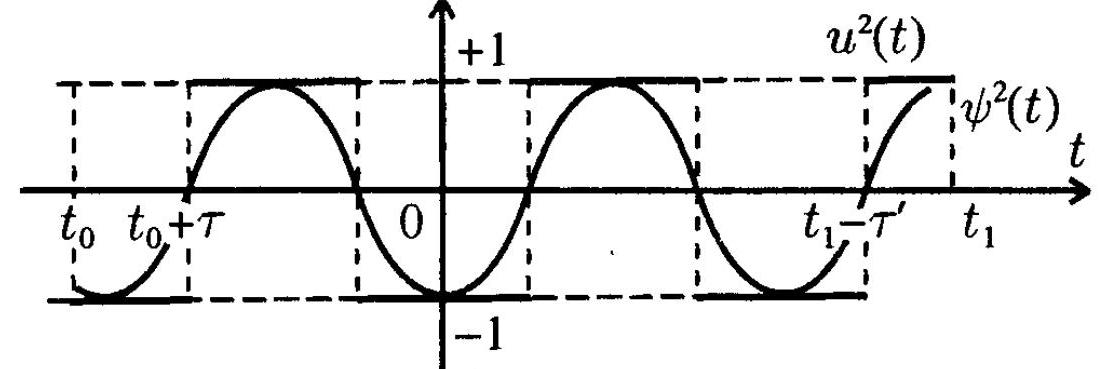
\includegraphics[max width=1.0\textwidth]{images/bo_d547okref24c73bgfch0_163_182_0_1099_369_0.jpg}
\end{center}
\hspace*{3em} 

Рис. 55

В соответствии с этим управление \({u}^{2}\left( t\right)\) , удовлетворяющее условию максимума (12.3), на отрезке времени \(\left\lbrack  {{t}_{0},{t}_{0} + \tau }\right\rbrack  ,\tau \leq  \pi\) , может равняться либо \(+1\) , либо \(-1\) , затем оно меняет свой знак несколько раз через промежуток времени \(\pi\) и, наконец, на от- резке времени \(\left\lbrack  {{t}_{1} - {\tau }^{\prime },{t}_{1}}\right\rbrack  ,{\tau }^{\prime } \leq  \pi\) также может равняться либо \(+1\) , либо \(-1\) .

В фазовой плоскости \({E}^{2}\) построим кривые, по которым про- исходит движение траектории \(\mathbf{x}\left( t\right)\) уравнения (12.1) при управ- лении \({u}^{2}\left( t\right)  =  + 1\) и при \({u}^{2}\left( t\right)  =  - 1\) . Если \({u}^{2}\left( t\right)  =  + 1\) , то уравнение (12.1) имеет вид

\[
\left\{  \begin{array}{l} {\dot{x}}^{1} = {x}^{2}, \\  {\dot{x}}^{2} =  - {x}^{1} + 1. \end{array}\right. \tag{12.4}
\]

Деля первое уравнение на второе и интегрируя, получаем в плоскости \({E}^{2}\) семейство кривых

\[
{\left( {x}^{1} - 1\right) }^{2} + {\left( {x}^{2}\right) }^{2} = {c}^{2},
\]

где с — константа, определяемая начальной точкой траектории. Эти кривые являются окружностями с центром в точке (1,0) — тип 1. Они изображены на рис. 56.

Движение по окружностям происходит по часовой стрел- ке с постоянной угловой скоростью, причем полный оборот по

\[
\mathbf{x}\left( t\right)  = \left( {1 + c\cos \left( {\varphi  - t}\right) ,c\sin \left( {\varphi  - t}\right) }\right) .
\]

\begin{center}
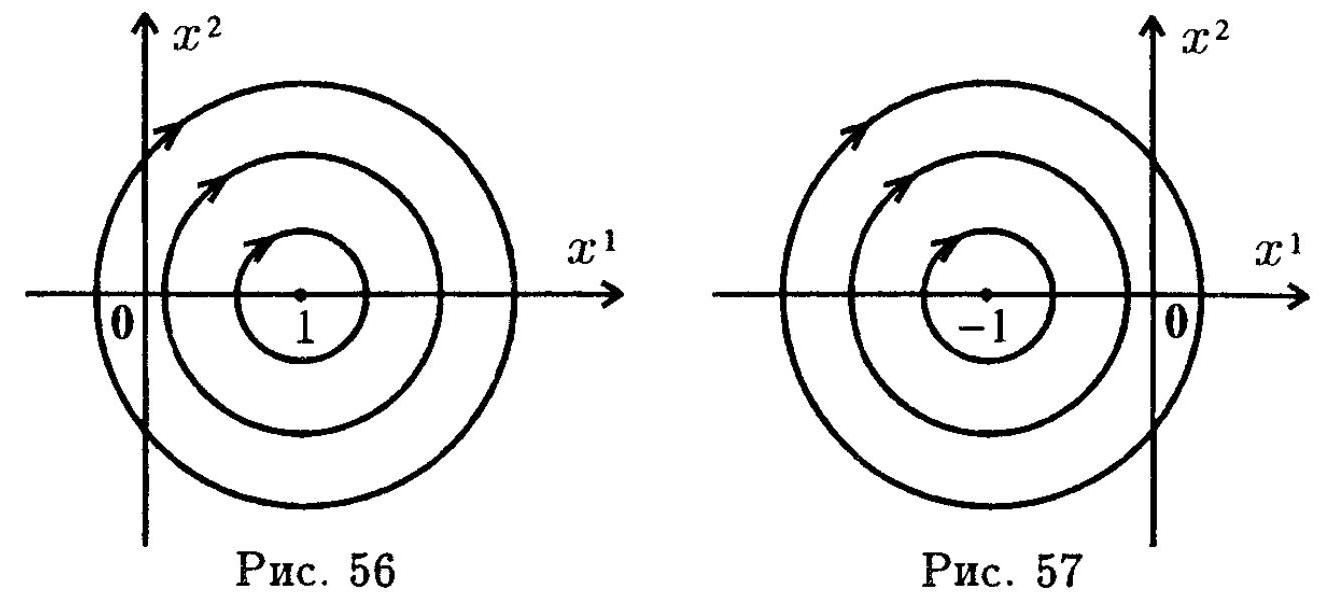
\includegraphics[max width=1.0\textwidth]{images/bo_d547okref24c73bgfch0_164_63_0_1327_597_0.jpg}
\end{center}
\hspace*{3em} 

окружности совершается за время 2π. Это определяется тем, что произвольное решение х(t) уравнения (12.1) имеет вид

Аналогичным образом получаем, что при \({u}^{2}\left( t\right)  =  - 1\) движение фазовой точки \(\mathbf{x}\left( t\right)\) происходит по окружностям с центром в точке \((-1,0)\) — тип 2 — также по часовой стрелке с постоянной угловой скоростью, причем полный оборот по окружности со- вершается за время \(2\pi\) . Таким образом, в те моменты времени \(t\) , когда \({u}^{2}\left( t\right)  =  + 1\) , фазовая точка \(\mathbf{x}\left( t\right)\) движется по окружностям типа 1, изображенным на рис. 56, а в те моменты времени \(t\) , когда \({u}^{2}\left( t\right)  =  - 1\) , фазовая точка \(\mathbf{x}\left( t\right)\) движется по окружностям типа 2, изображенным на рис. 57.

Для решения задачи синтеза оптимального управления по- ступим следующим образом. Найдем все точки фазовой плоскос- ти, из которых можно перейти в соответствии с принципом мак- симума в начало координат х = 0 без переключений управления \({u}^{2}\left( t\right)\) . При этом время перехода \(T = {t}_{1} - {t}_{0}\) не может быть больше \(\pi\) . При \({u}^{2}\left( t\right)  \equiv   + 1\) можно перейти в начало координат хе 0 из всех точек полуокружности типа 1, соединяющей точки (0,0) и (2,0). Oна изображена на рис. 58. При этом из точки (2,0) время перехода \(T = \pi\) . Аналогично при \({u}^{2}\left( t\right)  \equiv   - 1\) можно перейти в начало координат х = 0 из всех точек полуокружности типа 2, соединяющей точки \(\left( {0,0}\right)\) и (-2,0) (см. рис. 58).

Найдем теперь все точки фазового пространства, из кото- рых можно перейти в соответствии с принципом максимума в начало координат с одним переключением управления \({u}^{2}\left( t\right)\) . Если управление \({u}^{2}\left( t\right)\) сначала равняется -1, а затем +1, то траектория \(\mathbf{x}\left( t\right)\) идет сначала по окружности типа 2,а затем по окружности типа 1. Но единственная полуокружность типа 1, по которой можно прийти в начало координат без переключе- ния, изображена на рис. 58. Таким образом, нужно найти все точки фазовой плоскости, из которых можно попасть на эту полуокружность типа 1 по всевозможным окружностям типа 2. При этом двигаться по таким окружностям точка х(t) может не больше, чем время π. Все такие точки изображены на рис. 59. Аналогично строят все точки, из которых можно перейти в \(\mathbf{x} = \mathbf{0}\) c управлением и, \({u}_{2}\left( t\right)\) ,принимающим значения сначала +1, а затем -1. Такие точки также изображены на рис. 59.

Рис. 59

\begin{center}
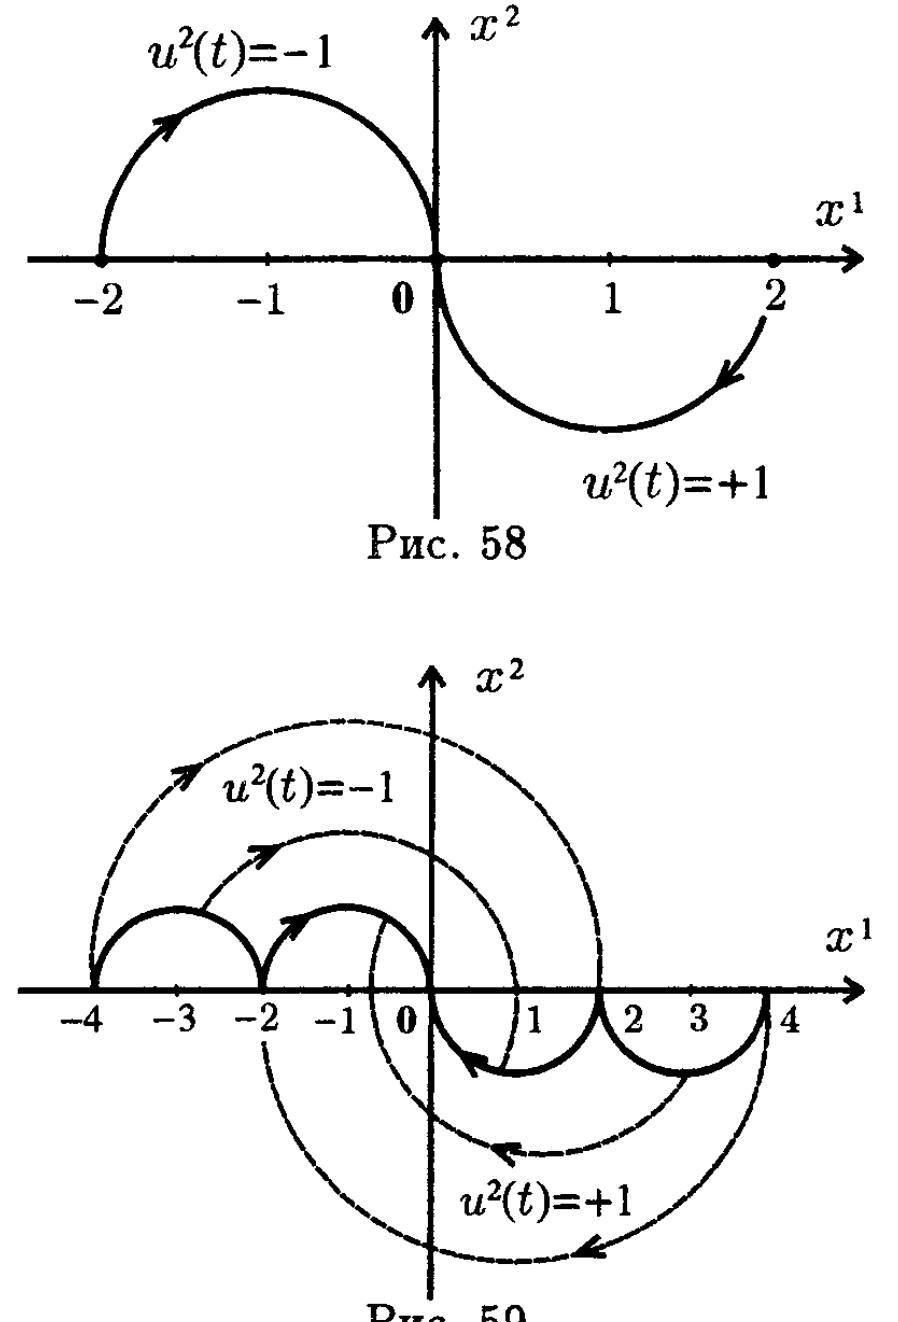
\includegraphics[max width=0.8\textwidth]{images/bo_d547okref24c73bgfch0_165_288_0_898_1322_0.jpg}
\end{center}
\hspace*{3em} 

Найдем теперь все точки, из которых можно перейти в х = 0 c двумя переключениями управления \({u}^{2}\left( t\right)\) . Пусть \({u}^{2}\left( t\right)\) сначала принимает значение +1, затем -1 и в конце движения снова +1. Тогда время движения с управлением и \({u}^{2}\left( t\right)  =  - 1\) долж- но равняться π. Таким образом, к точкам, изображенным на рис. 58, нужно добавить еще те точки плоскости, из которых можно перейти с управлением и па 1 на полуокружность, соединяющую точки (0,—4) и (0,—2), за время, меньшее или равное \(\pi\) . Аналогично находим точки, из которых возможен переход в начало координат с управлением \({u}^{2}\left( t\right)\) ,принимающим последовательно значения —1,+1,-1.

\begin{center}
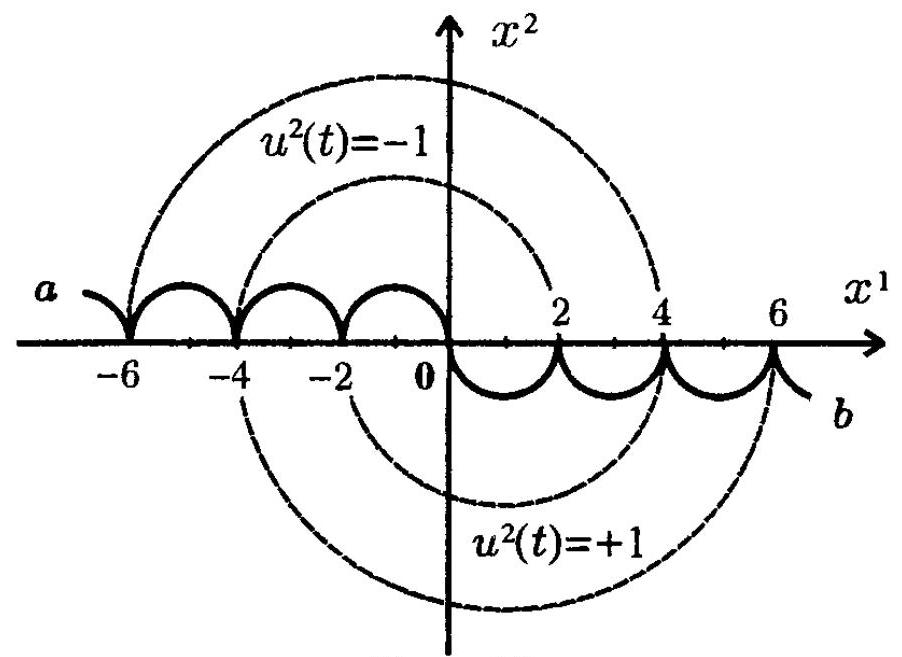
\includegraphics[max width=0.8\textwidth]{images/bo_d547okref24c73bgfch0_166_286_0_902_657_0.jpg}
\end{center}
\hspace*{3em} 

Рис. 60

Множество всех точек, из которых возможен переход в нача- ло координат не более чем с двумя переключениями, изображено на рис. 60. Продолжая этот процесс далее, для каждой точки фа- зовой плоскости \({\mathbf{x}}_{0} \in  {E}^{2}\) построим управление \(\mathbf{u}\left( t\right)  = \left( {0,{u}^{2}\left( t\right) }\right)\) и соответствующее решение \(\mathbf{x}\left( t\right)\) , переводящее эту точку \({\mathbf{x}}_{0}\) в начало координат \(\mathbf{x} = \mathbf{0}\) , причем пара \(\mathbf{u}\left( t\right) ,\mathbf{x}\left( t\right)\) удовлетворяет принципу максимума Понтрягина (рис. 60). Следовательно, та- кое управление \(\mathbf{u}\left( t\right)\) оптимально. Оптимальное управление \({u}^{2}\left( t\right)\) меняет свой знак на кривой \(a0b\) , состоящей из полуокружностей единичного радиуса. При этом выше этой кривой и на ее час- ти \(a0\) оптимальное управление имеет вид \({u}^{2}\left( t\right)  =  - 1\) , а ниже кривой \(a0b\) и на ее части \(0b\) — вид \({u}^{2}\left( t\right)  =  + 1\) . Теперь если уравнение (12.1) описывает поведение какого-либо технического объекта, то для него несложно построить автоматический опти- мальный регулятор, который по фазовому состоянию объекта \(\mathbf{x}\) будет вырабатывать оптимальное управление \(\mathbf{u}\left( \mathbf{x}\right)  = \left( {0,{u}^{2}\left( \mathbf{x}\right) }\right)\) . Действительно, если фазовая точка \(\mathbf{x}\) лежит выше кривой \(a0b\) или на ее части \(a0\) , то автоматический регулятор должен вы- работать управление \({u}^{2}\left( \mathbf{x}\right)  =  - 1\) , а если точка \(\mathbf{x}\) лежит ниже кривой \(a0b\) или на ее части \(0b\) , то регулятор должен вырабо- тать управление \({u}^{2}\left( \mathbf{x}\right)  =  + 1\) . Таким образом построенная функ- ция \(\mathbf{u}\left( \mathbf{x}\right)  = \left( {0,{\mathbf{u}}^{2}\left( \mathbf{x}\right) }\right)\) называется оптимальной синтезирующей функцией.

Заметим, что теперь не важно, в какую начальную точку хо под действием случайных сил будет заброшен маятник. Авто- матический регулятор, вырабатывающий функцию \({u}^{2}\left( \mathbf{x}\right)\) ,при- ведет его в состояние покоя за наименьшее время. Более того, в процессе этого перехода из точки х 0 в точку х = 0 на маятник может снова подействовать какая-либо случайная сила и забро- сить его в новую точку х, при этом автоматический регулятор будет переводить маятник из этой точки х 0, в состояние покоя за наименьшее время. Если бы регулятор вырабатывал опти- мальное управление в виде \({u}^{2}\left( t\right)\) для заданной начальной точки \({\mathbf{x}}_{0}\) , то такой учет текущих возмущений был бы невозможен.

Отсюда ясно, что с практической точки зрения очень важ- но уметь строить для управляемого объекта синтезирующую функцию \(\mathbf{u}\left( \mathbf{x}\right)\) . Для большого класса линейных задач быстро- действия такую синтезирующую функцию и(x) всегда можно построить с помощью принципа максимума Понтрягина та- ким же образом, как и для маятника, описываемого уравнением (12.1).

\section*{12.2. Единственность оптимального управления}

В лекции 10 остался невыясненным вопрос: при каких усло- виях на задачу быстродействия для заданного начального значе- ния сопряженной функции \(\mathbf{\psi }\left( {t}_{0}\right)  \in  S\) существует единственная пара \(\mathbf{u}\left( t\right) ,\mathbf{x}\left( t\right)\) , удовлетворяющая принципу максимума Понтря- гина? В соответствии со схемой, приведенной на рис. 40, неод- нозначность может возникнуть лишь в двух местах. Начальное значение фазового вектора \(\mathbf{x}\left( {t}_{0}\right) \in  {M}_{0}\) может определяться из условия трансверсальности на множестве \({M}_{0}\)

\[
\left\langle  {\mathbf{x}\left( {t}_{0}\right) ,\mathbf{\psi }\left( {t}_{0}\right) }\right\rangle   = c\left( {{M}_{0},\mathbf{\psi }\left( {t}_{0}\right) }\right) \tag{12.5}
\]

неединственным образом,также и управление \(\mathbf{u}\left( t\right)  \in  U\left( t\right)\) может определяться из условия максимума

\[
\langle \mathbf{u}\left( t\right) ,\mathbf{\psi }\left( t\right) \rangle  = c\left( {U,\mathbf{\psi }\left( t\right) }\right) \tag{12.6}
\]

неединственным образом. Заметим, что единственность управ- ления \(\mathbf{u}\left( t\right)\) здесь понимается в том смысле, что две измеримые функции равны на некотором отрезке времени, если они совпа- дают почти всюду на этом отрезке.

Рассмотрим, когда на этих этапах будет однозначное соот- ветствие и, следовательно, когда данному значению \(\mathbf{\psi }\left( {t}_{0}\right)  \in  S\) будет соответствовать единственная пара и(t), х(t), удовлетво- ряющая принципу максимума.

Первая теорема единственности. Пусть задано началь- ное значение \(\psi \left( {t}_{0}\right)  \in  {Su}\) coomветствующее решение \(\psi \left( t\right)\) co- пряженной системы на отрезке времени I = [힌, t1]. Предполо- жим,что опорная функция с \(\left( {{M}_{0},\mathbf{\psi }}\right)\) является дифференцируе- мой по ψ в точке ψ(и), т. е. в этой точке существует гради- ент функции с \(\left( {{M}_{0}, \cdot  }\right)  : {E}^{n} \rightarrow  {E}^{1}\) . Далее, предположим, что для noumu всех t ∈ I опорная функция с \(\left( {U,\psi }\right)\) дифференцируема no \(\mathbf{\psi }\) в точке \(\mathbf{\psi }\left( t\right)\) . Toгда соответствующая пара и(t), \(\mathbf{x}\left( t\right)\) , удовлетворяющая принципу максимума Понтрягина, является единственной.

Доказательство. Геометрически дифференцируемость функции \(c\left( {{M}_{0},\mathbf{\psi }}\right)\) no \(\mathbf{\psi }\) в точке \(\mathbf{\psi }\left( {t}_{0}\right)\) означает,что опорное множество для множества \({M}_{0}\) в направлении \(\mathbf{\psi }\left( {t}_{0}\right)\) coстоит из единственной точки и эта точка есть вектор \(\frac{\partial c\left( {{M}_{0},\psi \left( {t}_{0}\right) }\right) }{\partial \psi }\) . Дока- зательство этого факта приведено в разделе Д5 дополнений. Точно так же дифференцируемость функции \(c\left( {U,\mathbf{\psi }}\right)\) по \(\mathbf{\psi }\) в точке \(\psi \left( t\right)\) означает, что опорное множество для множества \(U\) cocorout из единственной точки и эта точка есть \(\frac{\partial c\left( {U,\psi \left( t\right) }\right) }{\partial \psi }\) . Следовательно, из условия (12.5) определяется единственный вектор \(\mathbf{x}\left( {t}_{0}\right)  = \frac{\partial c\left( {{M}_{0},\psi \left( {t}_{0}\right) }\right) }{\partial \psi }\) , a из условия (12.6) определяется при почти всех t ∈ I единственный вектор \(\mathbf{u}\left( t\right)  = \frac{\partial c\left( {U,\psi \left( t\right) }\right) }{\partial \psi }\) . Теорема доказана.

Назовем множество F строго выпуклым, если любая его опорная гиперплоскость пересекается с ним в единственной точке.

Следствие. Пусть множество Мо строго выпукло и мно- жество U также строго выпукло для почти всех t ∈ I. Тогда для любого начального значения \(\mathbf{\psi }\left( {t}_{0}\right)  \in  S\) coomветствующая napa \(\mathbf{u}\left( t\right) ,\mathbf{x}\left( t\right) ,y\) довлетворяющая принципу максимума, явля- ется единственной.

Доказательство этого следствия непосредственно выте- кает из геометрического смысла дифференцируемости опорной функции.

\section*{12.3. Условие общности положения*}

Рассмотрим задачу быстродействия для объекта, описывае- мого уравнением

\[
\dot{\mathbf{x}} = A\mathbf{x} + \mathbf{u}, \tag{12.7}
\]

в случае, когда множество \(U\) ,задающее ограничения на управ- ление и(t), является выпуклым замкнутым ограниченным мно- гогранником из Е". При этом множества начальных состояний \({M}_{0}\) и конечных состояний \({M}_{1}\) будем, \(\operatorname{\text{ к }a}\) к и ранее, считать не- пустыми выпуклыми компактами из \({E}^{n}\) .

Напомним, что выпуклый замкнутый многогранник Q из Е" представляет собой пересечение конечного числа замкнутых по- лупространств, т.е.: задается конечным числом линейных нера- венств:

\[
Q = \left\{  {\mathbf{x} \in  {E}^{n} : \left\langle  {\mathbf{x},{\mathbf{b}}_{j}}\right\rangle   \leq  {a}_{j},j = 1,2,\ldots ,s}\right\}  .
\]

Случай, когда множество U — выпуклый замкнутый ограни- ченный многогранник, представляет большой интерес, посколь- ку он часто встречается в приложениях. Этот случай является достаточно общим, поскольку любой выпуклый компакт U из \({E}^{n}\) можно сколь угодно точно приблизить в хаусдорфовой мет- рике выпуклым замкнутым ограниченным многогранником Q.

Так как произвольная гиперплоскость

\[
\Gamma  = \left\{  {\mathbf{x} \in  {E}^{n} : \langle \mathbf{x},\mathbf{b}\rangle  = a}\right\}  ,\;\mathbf{b} \neq  0
\]

может быть представлена в виде

\[
\Gamma  = \left\{  {\mathbf{x} \in  {E}^{n} : \langle \mathbf{x},\mathbf{b}\rangle  \leq  a,\langle \mathbf{x}, - \mathbf{b}\rangle  \leq   - a}\right\}  ,
\]

то гиперплоскость является выпуклым замкнутым многогран- ником. Отсюда следует, что любое опорное множество \({Q}^{\prime }\) вы- пуклого замкнутого многогранника \(Q\) снова является выпуклым замкнутым многогранником. Опорные множества многогранни- ка \(Q\) будем называть его гранями. Таким образом, произволь- ная грань \({Q}^{\prime }\) многогранника \(Q\) , если она не совпадает с самим многогранником \(Q\) , является многогранником меньшей размер- ности, чем \(Q\) (определение размерности выпуклого множества см. в разделе Д7 дополнений). При этом нетрудно видеть, что все грани многогранни- ка \({Q}^{\prime }\) являются также гра- нями исходного многогранни- ка \(Q\) . В случае, когда выпук- лый замкнутый многогранник \(Q\) ограничен, у него обяза- тельно существует конечное число граней нулевой размер- ности, т.е. граней, состоящих из одной точки. Такие грани называют вершинами многогранника \(Q\) . Грани, имеющие еди- ничную размерность, называют ребрами многогранника \(Q\) . Ес- ли многогранник \(Q\) ограничен и \({q}_{1},{q}_{2},\ldots ,{q}_{s}\) — его вершины, то многогранник \(Q\) совпадает с выпуклой оболочкой своих вершин, а каждое его ребро \(w\) является выпуклой оболочкой каких-то двух соседних вершин (рис. 61), т.е. является отрезком.

\HRule

*Данный раздел содержит классические результаты линейной теории опти- мального управления [1], дополняющие содержание этой и предыдущей лекций, и был добавлен в рукопись С.М. Асеевым.

\HRule

\begin{center}
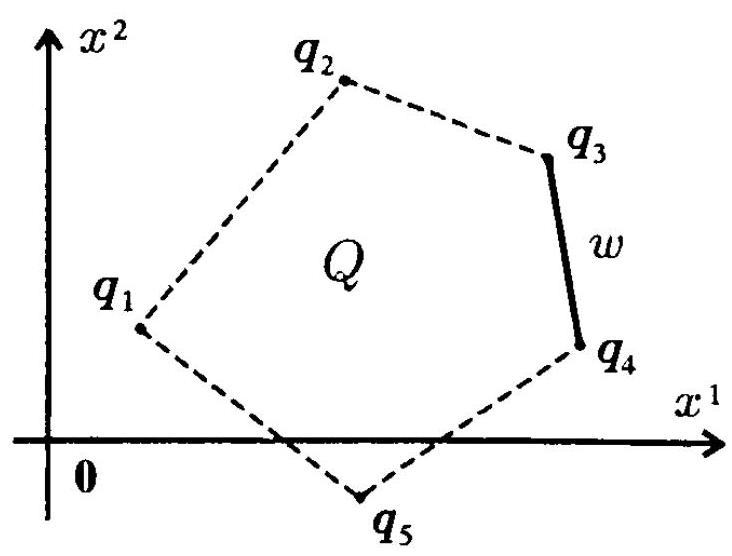
\includegraphics[max width=0.7\textwidth]{images/bo_d547okref24c73bgfch0_170_737_12_732_556_0.jpg}
\end{center}
\hspace*{3em} 

Рис. 61

Пусть ребро w является выпуклой оболочкой вершин \({q}_{i}\) и \({\mathbf{q}}_{j}\) , т.е. \(w = \operatorname{conv}\left\{  {{\mathbf{q}}_{i},{\mathbf{q}}_{j}}\right\}\) . Тогда будем говорить, что вектор \(v = \lambda \left( {{q}_{i} - {q}_{j}}\right)\) ,где \(\lambda  \neq  0\) ,шмеет направление ребра w много- гранника \(Q\) .

В дальнейшем будем предполагать, что коэффициенты урав- нения (12.7) и расположение выпуклого замкнутого ограничен- ного многогранника \(U\) в пространстве Е" удовлетворяют усло- вию общности положения, которое состоит в том, что если вектор v имеет направление одного из ребер многогранника U, TO BEKTOPLI

\[
v,{Av},\ldots ,{A}^{n - 1}v \tag{12.8}
\]

линейно независимы.

Поясним геометрический смысл условия общности положе- ния. Для этого нам потребуется понятие инвариантного подпро- странства.

Будем говорить, что линейное подпространство \(L\) простран- ства \({E}^{n}\) является инвариантным относительно преобразования* \(A\) , если для любого вектора \(\mathbf{x} \in  L\) вектор \(A\mathbf{x}\) снова принадлежит подпространству \(L\) . Подпространство \(L\) называется собствен- ным, если оно не совпадает со всем пространством \({E}^{n}\) и не состоит только из нуля. Легко видеть, что отличный от нуля вектор \(\mathbf{x}\) принадлежит некоторому собственному инвариантно- му относительно преобразования \(A\) подпространству \(L\) в том и только в том случае, когда векторы

\[
\mathbf{x},A\mathbf{x},\ldots ,{A}^{n - 1}\mathbf{x}
\]

\HRule

*Под преобразованием А здесь понимается отображение, порожденное матрицей A и ставящее в соответствие каждому вектору х из Е" его образ Ах.

\HRule

линейно зависимы.

Таким образом, выполнение условия общности положения означает, что никакой вектор v, имеющий направление какого- либо ребра многогранника \(U\) ,не принадлежит никакому собст- венному подпространству, инвариантному относительно преоб- разования \(A\) .

Пусть векторы \({\mathbf{u}}_{1},{\mathbf{u}}_{2},\ldots ,{\mathbf{u}}_{m}\) являются вершинами многогранника \(U\). Так как любой вектор \(\mathbf{v}\), имеющий направление некоторого ребра \(\gamma\) многогранника \(U\), имеет вид
\[
\mathbf{v} = \lambda \left( {\mathbf{u}}_{i} - {\mathbf{u}}_{j}\right),
\]
где \(\lambda \neq 0\) и \({\mathbf{u}}_{i},{\mathbf{u}}_{j}\) -- соответствующие вершины, то условие общности положения, очевидно, выполняется, если все определители матриц, составленных из столбцов \({\mathbf{u}}_{i} - {\mathbf{u}}_{j}, A\left( {\mathbf{u}}_{i} - {\mathbf{u}}_{j}\right), \ldots, {A}^{n-1}\left( {\mathbf{u}}_{i} - {\mathbf{u}}_{j}\right)\) при \(i \neq j\), отличны от нуля. Нетрудно видеть, что для любой матрицы \(A\) и для любого выпуклого замкнутого ограниченного многогранника \(U\) всегда можно так сколь угодно мало изменить элементы матрицы \(A\), что все такие определители будут отличны от нуля и, следовательно, будет выполняться условие общности положения. Если же условие общности положения выполняется, то, поскольку выпуклый многогранник \(U\) имеет конечное число ребер, это условие нельзя нарушить произвольно малым изменением элементов матрицы \(A\) и вершин многогранника \(U\).

Таким образом, условие общности положения не является обременительным, поскольку оно не выполняется только в исключительных случаях, а его выполнение всегда можно обеспечить малым изменением элементов матрицы \(A\). Кроме того, это свойство параметров управляемой системы (коэффициентов уравнения (12.7) и координат вершин многогранника \(U\)) является устойчивым относительно малых возмущений.

Как показывает следующий результат, выполнение условия общности положения гарантирует, что по любому нетривиальному решению \(\psi \left( t\right)\) сопряженной системы (11.2) единственным образом определяется управление \(\mathbf{u}\left( t\right)\), удовлетворяющее условию максимума (11.3), как кусочно постоянная функция, принимающая значения в вершинах многогранника \(U\).

Теорема о конечном числе переключений. Пусть выполнено условие общности положения и \(\psi(t)\) -- произвольное ненулевое решение сопряженной системы (11.2) на отрезке времени \(I = \left[ t_{0},t_{1}\right]\). Тогда, за исключением, быть может, конечного числа моментов времени \(t\), условие максимума (11.3) однозначно определяет значение управления \(\mathbf{u}(t)\) как одну из вершин многогранника \(U\). При этом данное управление \(\mathbf{u}(t)\) может иметь не более конечного числа точек разрыва.

Доказательство. Рассмотрим условие максимума

\[
\langle u,\psi \left( t\right) \rangle  = c\left( {U,\psi \left( t\right) }\right) \tag{12.9}
\]

как уравнение относительно неизвестного вектора и с U при фиксированном t. Тогда в силу линейности скалярного произ- ведения функция \(\langle \mathbf{u},\mathbf{\psi }\left( t\right) \rangle\) переменной и либо постоянна на \(U\) , либо достигает своего максимума на какой-то грани и/ много- гранника \(U\) paзмерности меньшей, чем размерность многогран- ника U. Это может быть либо грань нулевой размерности, т.е. вершина, либо некоторая грань \({U}^{\prime }\) ненулевой размерности. В последнем случае функция \(\langle \mathbf{u},\mathbf{\psi }\left( t\right) \rangle\) постоянна на \({U}^{\prime }\) и,следо- вательно, постоянна на некотором ребре (грани единичной раз- мерности) \(w\) многогранника \({U}^{\prime }\) . Поскольку каждая грань мно- гогранника \({U}^{\prime }\) является также гранью многогранника \(U\) ,то это ребро w является ребром многогранника U. Итак, либо единст- венной точкой максимума функции \(\langle \mathbf{u},\mathbf{\psi }\left( t\right) \rangle\) является некоторая вершина многогранника \(U\) , либо максимум достигается во всех точках некоторого ребра w этого многогранника. Покажем, что в силу условия общности положения этот максимум может до- стигаться на каком-либо ребре w только для конечного числа значений t.

Действительно, предположим противное, т.е. предположим, что максимум функции \(\langle \mathbf{u},\mathbf{\psi }\left( t\right) \rangle\) достигается на ребре много- гранника \(U\) для бесконечного числа значений t. Тогда, посколь- ку число ребер многогранника \(U\) конечно, то найдется ребро \(w\) ,на котором максимум достигается в счетном числе моментов времени \({\tau }_{1},{\tau }_{2},\ldots  \in  I\) . Пусть это ребро w образовано вершинами \({\mathbf{u}}^{\prime }\) и и отда ⟨ \({\mathbf{u}}^{\prime },\mathbf{\psi }\left( {\tau }_{i}\right) \rangle  = \left\langle  {{\mathbf{u}}^{\prime \prime },\dot{\mathbf{\psi }}\left( {\tau }_{i}\right) }\right\rangle  ,i = 1,2,\ldots\) Cледователь- но,для вектора v = u' - u", имеющего направление ребра w,

IMMeeM

\[
\left\langle  {v,\psi \left( {\tau }_{i}\right) }\right\rangle   = 0\;\left( {i = 1,2,\ldots }\right) .
\]

Поскольку функция \(\mathbf{\psi }\left( t\right)\) как решение линейной системы диффе- ренциальных уравнений (11.2) является аналитической, отсюда следует, что \(\langle \mathbf{v},\mathbf{\psi }\left( t\right) \rangle  = 0\) для всех точек \(t \in  I\) . Продиффе- ренцировав последовательно \(n - 1\) pa3 тождество \(\langle \mathbf{v},\mathbf{\psi }\left( t\right) \rangle  \equiv  0\) во внутренних точках отрезка \(I\) и воспользовавшись тем,что функция \(\mathbf{\psi }\left( t\right)\) — решение сопряженной системы (11.2), получим следующие \(n\) тождеств на \(I\) :

\[
\langle \mathbf{v},\mathbf{\psi }\left( t\right) \rangle  \equiv  0\;\forall t \in  I,
\]

\[
\langle A\mathbf{v},\mathbf{\psi }\left( t\right) \rangle  \equiv  0\;\forall t \in  I,
\]

\[
\text{ ............................ }
\]

\[
\left\langle  {{A}^{n - 1}\mathbf{v},\mathbf{\psi }\left( t\right) }\right\rangle   \equiv  0\;\forall t \in  I.
\]

В силу условия общности положения векторы (12.8) линейно независимы. Cледовательно, \(\mathbf{\psi }\left( t\right)  = \mathbf{0}\) на \(I\) ,что противоречит предположению о нетривиальности функции \(\mathbf{\psi }\left( t\right)\) .

Итак, доказано, что, за исключением, быть может, конечно- го числа значений \(t\) , ynpaвление \(\mathbf{u}\left( t\right)\) однозначно определяется функцией ψ(t) из условия максимума (12.9) как некоторая вер- шина многогранника U. Пусть ти < то < ... < тише иск ситек сейств ключительные значения времени, при которых управление и не определяется однозначно из условия максимума (12.9). Дока- жем,что на каждом интервале \({J}_{i} = \left( {{\tau }_{i},{\tau }_{i + 1}}\right) ,i = 1,2,\ldots ,N - 1\) управление \(u\left( t\right)\) постоянно. Пусть \({u}_{1},\ldots ,{u}_{m}\) - все вершины многогранника \(U\) . Обозначим через \({M}_{i,j} = \left\{  {t \in  {J}_{i} : u\left( t\right)  = {u}_{j}}\right\}\) , \(i = 1,\ldots ,N - 1,j = 1,\ldots ,m\) coboxрипность тех точек множес- тва \({J}_{i}\) ,в которых значением управления и(t) является верши- на \({\mathbf{u}}_{j}\) . При этом некоторые из множеств Ми, j могут оказаться пустыми. Очевидно, множества Ми, j попарно не пересекаются и \(\mathop{\bigcup }\limits_{{j = 1,\ldots ,m}}{M}_{i,j} = {J}_{i}\)

Выберем какое-либо непустое множество \({M}_{i,r}\) . Пусть \(\tau\) — не- которая точка множества Ми,г. В силу условия максимума (12.9) и определения множества \({M}_{i,r}\) имеем \(\left\langle  {{\mathbf{u}}_{r},\mathbf{\psi }\left( \tau \right) }\right\rangle   > \left\langle  {{\mathbf{u}}_{j},\mathbf{\psi }\left( \tau \right) }\right\rangle\) при \(j \neq  r\) , a в силу непрерывности функции \(\psi \left( t\right)\) cymeствует \(\varepsilon  > 0\) такое, что неравенство \(\left\langle  {{\mathbf{u}}_{r},\mathbf{\psi }\left( t\right) }\right\rangle   > \left\langle  {{\mathbf{u}}_{j},\mathbf{\psi }\left( t\right) }\right\rangle\) выполняется для всех \(t \in  \left\{  {t \in  {J}_{i} : \left| {t - \tau }\right|  < \varepsilon }\right\}  ,j \neq  r\) . Таким образом,множество \({M}_{i,r}\) является открытым. C другой стороны,это множество \({M}_{i,r}\) является замкнутым в \({J}_{i}\) . Действительно, пусть т — предельная точка множества \({M}_{i,r}\) ,принадлежащая множеству \({J}_{i}\) . Это озна- чает,что найдется такая последовательность точек \(\left\{  {\tau }_{k}\right\}   \in  {M}_{i,r}\) , \(k = 1,2,\ldots\) ,что \({\tau }_{k} \rightarrow  \tau\) . В силу определения множества \({M}_{i,r}\) вы- полняется равенство \(\left\langle  {{\mathbf{u}}_{r},\mathbf{\psi }\left( {\tau }_{k}\right) }\right\rangle   = c\left( {U,\mathbf{\psi }\left( {\tau }_{k}\right) }\right)\) . B силу непрерыв- ности скалярного произведения, непрерывности опорной функ- ции и непрерывности функции \(\mathbf{\psi }\left( t\right)\) , переходя в последнем ра- венстве к пределу при \(k \rightarrow  \infty\) ,получаем \(\left\langle  {{\mathbf{u}}_{r},\mathbf{\psi }\left( \tau \right) }\right\rangle   = c\left( {U,\mathbf{\psi }\left( \tau \right) }\right)\) . Cледовательно, \(\tau  \in  {M}_{i,r}\) . Таким образом, множество \({M}_{i,r}\) за- мкнуто в \({J}_{i}\) . Поскольку интервал \({J}_{i} = \left( {{\tau }_{i},{\tau }_{i + 1}}\right)\) - множество связное, а выбранное непустое множество \({M}_{i,r}\) одновременно открыто и замкнуто в \({J}_{i}\) , to \({M}_{i,r} = {J}_{i}\) . Oстальные же множества \({M}_{i,j}\) при \(j \neq  r\) пусты. Итак, на каждом интервале \({J}_{i}\) управление \(\mathbf{u}\left( t\right)\) постоянно. Теорема доказана.

Поскольку изменение значения управления на множестве ну- левой меры не оказывает никакого влияния на траекторию сис- темы, то при выполнении условия общности положения в данной задаче быстродействия в качестве допустимых управлений мож- но рассматривать класс кусочно постоянных и непрерывных слева управлений. Этот класс управлений состоит из функций, имеющих не более конечного числа точек разрыва (называемых точками переключения), постоянных на каждом интервале не- прерывности и имеющих в каждой точке разрыва своим значе- нием предел слева. Действительно, 'если в исходной задаче вы- полняется условие общности положения и система управляема из \({M}_{0}\) на \({M}_{1}\) , то в силу теоремы существования оптимально- го управления (см. лекцию 9) оптимальное по быстродействию управление существует в классе измеримых управлений. Далее, оптимальное управление удовлетворяет принципу максимума Понтрягина. Следовательно, в силу теоремы о конечном числе переключений, переопределив, если это необходимо, оптималь- ное управление на множестве нулевой меры, можно считать его кусочно постоянным и непрерывным слева.

В некоторых важных случаях условие общности положе- ния позволяет гарантировать оптимальность управления, удов- летворяющего принципу максимума Понтрягина, и единствен- ность оптимального управления.

Вторая теорема единственности. Пусть выполнено условие общности положения. Предположим, что управления \({u}_{1}\left( t\right)\) и \({u}_{2}\left( t\right)\) переводят систему из точки \({\mathbf{x}}_{0}\) в точку \({\mathbf{x}}_{1}\) на отрезке времени \(I = \left\lbrack  {{t}_{0},{t}_{1}}\right\rbrack\) . Предположим также, что каж- дое из этих управлений удовлетворяет принципу максимума Понтрягина. Тогда управления \({u}_{1}\left( t\right)\) и \({u}_{2}\left( t\right)\) совпадают.

Доказательство. Поскольку начальное и конечное состо- яния траекторий, соответствующих управлениям \({u}_{1}\left( t\right)\) и \({u}_{2}\left( t\right)\) , совпадают, то в силу формулы Коши (см. лекцию 6) имеем

\[
{\mathbf{x}}_{1} = {e}^{\left( {{t}_{1} - {t}_{0}}\right) A}{\mathbf{x}}_{0} + {\int }_{{t}_{0}}^{{t}_{1}}{e}^{\left( {{t}_{1} - s}\right) A}{\mathbf{u}}_{1}\left( s\right) {ds} =
\]

\[
= {e}^{\left( {{t}_{1} - {t}_{0}}\right) A}{x}_{0} + {\int }_{{t}_{0}}^{{t}_{1}}{e}^{\left( {{t}_{1} - s}\right) A}{u}_{2}\left( s\right) {ds}.
\]

Следовательно,

\[
{\int }_{{t}_{0}}^{{t}_{1}}{e}^{\left( {{t}_{1} - s}\right) A}\left( {{u}_{1}\left( s\right)  - {u}_{2}\left( s\right) }\right) {ds} = 0. \tag{12.10}
\]

Пусть управлению \({u}_{1}\left( t\right)\) соответствует в силу принципа мак- симума Понтрягина сопряженная функция \({\mathbf{\psi }}_{1}\left( t\right)\) . Умножив ска- лярно равенство (12.10) на вектор \({\psi }_{1}\left( {t}_{1}\right)\) , noлучаем

\[
{\int }_{{t}_{0}}^{{t}_{1}}\left\langle  {{\mathbf{u}}_{1}\left( s\right)  - {\mathbf{u}}_{2}\left( s\right) ,{e}^{\left( {{t}_{1} - s}\right) {A}^{ * }}{\psi }_{1}\left( {t}_{1}\right) }\right\rangle  {ds} = 0
\]

или (см. формулу (9.11))

\[
{\int }_{{t}_{0}}^{{t}_{1}}\left\langle  {{u}_{1}\left( s\right)  - {u}_{2}\left( s\right) ,{\psi }_{1}\left( s\right) }\right\rangle  {ds} = 0.
\]

Отсюда в силу условия максимума следует равенство

\[
{\int }_{{t}_{0}}^{{t}_{1}}\left( {c\left( {U,{\psi }_{1}\left( s\right) }\right)  - \left\langle  {{u}_{2}\left( s\right) ,{\psi }_{1}\left( s\right) }\right\rangle  }\right) {ds} = 0.
\]

Поскольку подынтегральное выражение в последнем равен- стве неотрицательно, то для почти всех t ∈ \(\left\lbrack  {{t}_{0},{t}_{1}}\right\rbrack\) для управле- ния \({u}_{2}\left( t\right)\) выполняется условие максимума с сопряженной функ- цией \({\psi }_{1}\left( t\right)\)

\[
\left\langle  {{\mathbf{u}}_{2}\left( t\right) ,{\psi }_{1}\left( t\right) }\right\rangle   = c\left( {U,{\psi }_{1}\left( t\right) }\right) ,
\]

отсюда в силу теоремы о конечном числе переключений полу- чаем, что \({u}_{1}\left( t\right)  = {u}_{2}\left( t\right)\) для почти всех t ∈ \(\left\lbrack  {{t}_{0},{t}_{1}}\right\rbrack\) . Теорема доказана.

Следствие. Пусть выполнено условие общности положе- ния. Тогда если система управляема из точки \({\mathbf{x}}_{0}\) в точку \({\mathbf{x}}_{1}\) , то оптимальное по быстродействию управление \(\mathbf{u}\left( t\right)\) сущест- вует и единственно.

Доказательство данного следствия непосредственно вы- текает из теоремы существования оптимального управления (см. лекцию 9) и второй теоремы единственности. Здесь изме- римые управления \({u}_{1}\left( t\right)\) и \({u}_{2}\left( t\right)\) считаются совпадающими, если \({\mathbf{u}}_{1}\left( t\right)  = {\mathbf{u}}_{2}\left( t\right)\) для почти всех \(t \in  \left\lbrack  {{t}_{0},{t}_{1}}\right\rbrack\) .

Вторая теорема о достаточных условиях оптимальности. Пусть выполнено условие общности положения, множество \(M_{0}\) состоит из единственной точки \(\mathbf{x}_{0}\), а множество \(M_{1}\) состоит из единственной точки \(\mathbf{0}\). Пусть, кроме того, \(\mathbf{0} \in U\) и начало координат не является вершиной многогранника \(U\). Тогда если управление \(\mathbf{u}(t)\) удовлетворяет принципу максимума Понтрягина на некотором отрезке времени \(I = \left[ t_{0},t_{1}\right]\), то оно оптимально и \(T = {t}_{1} - {t}_{0}\) -- время быстродействия.

Доказательство. Предположим противное, т.е. что существует такое допустимое управление \({u}_{2}\left( t\right)\), переводящее систему из точки \({\mathbf{x}}_{0}\) в начало координат на отрезке времени \({I}^{\prime } = \left\lbrack  {{t}_{0},{t}_{2}}\right\rbrack\), где \({t}_{2} < {t}_{1}\). Пусть \({\psi }_{1}\left( t\right)\) -- ненулевая сопряженная функция, соответствующая в силу принципа максимума Понтрягина управлению \({u}_{1}\left( t\right)\).

Поскольку управление \({u}_{1}\left( t\right)\) переводит точку \({\mathbf{x}}_{0}\) на отрезке времени \(I\) в начало координат, то в силу формулы Коши имеем

\[
{e}^{\left( {{t}_{1} - {t}_{0}}\right) A}{x}_{0} + {\int }_{{t}_{0}}^{{t}_{1}}{e}^{\left( {{t}_{1} - s}\right) A}{u}_{1}\left( s\right) {ds} =
\]

\[
= {e}^{\left( {{t}_{1} - {t}_{2}}\right) A}\left( {{e}^{\left( {{t}_{2} - {t}_{0}}\right) A}{x}_{0} + {\int }_{{t}_{0}}^{{t}_{1}}{e}^{\left( {{t}_{2} - s}\right) A}{u}_{1}\left( s\right) {ds}}\right)  = 0.
\]

Так как матрица \({e}^{\left( {{t}_{1} - {t}_{2}}\right) A}\) невырожденная, то из последнего равенства получаем

\[
{e}^{\left( {{t}_{2} - {t}_{0}}\right) A}{x}_{0} + {\int }_{{t}_{0}}^{{t}_{1}}{e}^{\left( {{t}_{2} - s}\right) A}{u}_{1}\left( s\right) {ds} = 0. \tag{12.11}
\]

Поскольку управление \({u}_{2}\left( t\right)\) переводит точку \({\mathbf{x}}_{0}\) на своем отрезке времени \({I}^{\prime } = \left\lbrack  {{t}_{0},{t}_{2}}\right\rbrack\) в начало координат, то в силу формулы Коши имеем

\[
{e}^{\left( {{t}_{2} - {t}_{0}}\right) A}{x}_{0} + {\int }_{{t}_{0}}^{{t}_{2}}{e}^{\left( {{t}_{2} - s}\right) A}{u}_{2}\left( s\right) {ds} = 0,
\]

откуда в силу равенства (12.11) получаем

\[
{\int }_{{t}_{0}}^{{t}_{2}}{e}^{\left( {{t}_{2} - s}\right) A}\left( {{u}_{1}\left( s\right)  - {u}_{2}\left( s\right) }\right) {ds} + {\int }_{{t}_{2}}^{{t}_{1}}{e}^{\left( {{t}_{2} - s}\right) A}{u}_{1}\left( s\right) {ds} = 0.
\]

Умножив скалярно последнее равенство на вектор \({\mathbf{\psi }}_{1}\left( {t}_{2}\right)\), получим

\[
{\int }_{{t}_{0}}^{{t}_{2}}\left\langle  {{u}_{1}\left( s\right)  - {u}_{2}\left( s\right) ,{\psi }_{1}\left( s\right) }\right\rangle  {ds} + {\int }_{{t}_{2}}^{{t}_{1}}\left\langle  {{u}_{1}\left( s\right) ,{\psi }_{1}\left( s\right) }\right\rangle  {ds} = 0. \tag{12.12}
\]

Далее, так как в силу условия максимума для почти всех \(t \in  \left\lbrack  {{t}_{0},{t}_{1}}\right\rbrack\) имеет место равенство \(\left\langle  {{\mathbf{u}}_{1}\left( t\right) ,{\mathbf{\psi }}_{1}\left( t\right) }\right\rangle   = c\left( {U,{\mathbf{\psi }}_{1}\left( t\right) }\right)\), то в равенстве (12.12) подынтегральное выражение в первом слагаемом неотрицательно и, следовательно, первое слагаемое также неотрицательно. Следовательно, второе слагаемое в равенстве (12.12) неположительно. С другой стороны, поскольку \(0 \in  U\), то

\[
c\left( {U,{\psi }_{1}\left( t\right) }\right)  \geq  0
\]

для всех значений \(t \in  \left\lbrack  {{t}_{0},{t}_{1}}\right\rbrack\) и, следовательно, \(\left\langle  {{\mathbf{u}}_{1}\left( t\right) ,{\mathbf{\psi }}_{1}\left( t\right) }\right\rangle   \geq  0\) для почти всех \(t \in  \left\lbrack  {{t}_{2},{t}_{1}}\right\rbrack\), откуда получаем, что второе слагаемое в равенстве (12.12) неотрицательно. Следовательно,

\[
{\int }_{{t}_{2}}^{{t}_{1}}\left\langle  {{\mathbf{u}}_{1}\left( s\right) ,{\mathbf{\psi }}_{1}\left( s\right) }\right\rangle  {ds} = {\int }_{{t}_{2}}^{{t}_{1}}c\left( {U,{\mathbf{\psi }}_{1}\left( s\right) }\right) {ds} = 0,
\]

откуда в силу условия \(0 \in U\) вытекает тождество \(c\left( {U,{\psi }_{1}\left( t\right) }\right)  \equiv  0\) на отрезке \(\left\lbrack  {{t}_{2},{t}_{1}}\right\rbrack\). Поскольку по условиям теоремы начало координат не является вершиной многогранника \(U\), то для каждого \(t \in  \left\lbrack  {{t}_{2},{t}_{1}}\right\rbrack\) найдется ребро многогранника \(U\), на котором скалярное произведение \(\langle \mathbf{u},{\mathbf{\psi }}_{1}\left( t\right) \rangle  = 0\) и, следовательно, постоянно. Поскольку число ребер многогранника \(U\) конечно, то найдется такое ребро \(w\), на котором скалярное произведение \(\langle \mathbf{u},{\mathbf{\psi }}_{1}\left( t\right) \rangle\) обращается в нуль для бесконечного числа моментов времени \(t \in  \left\lbrack  {{t}_{2},{t}_{1}}\right\rbrack\). Пусть вектор \(\mathbf{v}\) имеет направление этого ребра. Тогда в силу аналитичности функции \({\psi }_{1}\left( t\right)\) на отрезке \(\left\lbrack  {{t}_{2},{t}_{1}}\right\rbrack\) справедливо тождество \(\left\langle  {\mathbf{v},{\mathbf{\psi }}_{1}\left( t\right) }\right\rangle   \equiv  0\). Точно так же, как и в доказательстве теоремы о конечности числа переключений, продифференцировав последовательно \(n - 1\) раз это тождество во внутренних точках отрезка \(\left\lbrack  {{t}_{2},{t}_{1}}\right\rbrack\), в силу условия общности положения получаем противоречие с нетривиальностью сопряженной функции \({\psi }_{1}\left( t\right)\). Теорема доказана.

\section*{12.4. Задача}

1. Постройте синтез оптимального управления для задачи быстродействия в начало координат х = 0 для объекта, описы- ваемого уравнением

\[
\left\{  \begin{array}{l} {\dot{x}}^{1} = {x}^{2}, \\  {\dot{x}}^{2} = {u}^{2},\;\left| {u}^{2}\right|  \leq  1. \end{array}\right.
\]

\section*{ДОП ОЛНЕНИЯ}

\section*{Д1. Выпуклая оболочка множества}

Множество \(F \subset  {E}^{n}\) называется выпуклым, если для любых двух точек \({\mathbf{x}}_{1},{\mathbf{x}}_{2}\) отрезок, соединяющий эти точки, содер- жится в множестве \(F\) , или, что то же самое, если для любого числа \(0 \leq  \lambda  \leq  1\) выполняется условие \(\lambda {\mathbf{x}}_{1} + \left( {1 - \lambda }\right) {\mathbf{x}}_{2} \in  F\) .

Ясно, что пересечение любого числа выпуклых множеств, если оно непусто, снова будет множеством выпуклым.

Точка \(\mathbf{x}\) называется выпуклой комбинацией точек \({\mathbf{x}}_{1},\ldots ,{\mathbf{x}}_{m} \in  {E}^{n}\) , если существуют числа \({\lambda }_{i},i = 1,\ldots ,m\) , удов- летворяющие соотношениям \({\lambda }_{i} \geq  0,{\lambda }_{1} + \ldots  + {\lambda }_{m} = 1\) такие, что выполняется равенство

\[
\mathbf{x} = {\lambda }_{1}{\mathbf{x}}_{1} + \ldots  + {\lambda }_{m}{\mathbf{x}}_{m}.
\]
 (Д.1)

В этом смысле любая точка отрезка является выпуклой комби- нацией двух концов отрезка.

Лемма 1. Если множество F выпукло, то оно содержит любую выпуклую комбинацию своих точек.

Доказательство. Выпуклую комбинацию любых своих двух точек выпуклое множество содержит по определению. До- статочно положить \({\lambda }_{1} = \lambda ,{\lambda }_{2} = 1 - \lambda\) . Предположим по индук- ции, что множество \(F\) содержит выпуклую комбинацию любых \(m\) своих точек и \(m \geq  2\) . Возьмем произвольную выпуклую ком- бинацию

\[
\mathbf{x} = {\lambda }_{1}{\mathbf{x}}_{1} + \ldots  + {\lambda }_{m + 1}{\mathbf{x}}_{m + 1},\;{\lambda }_{i} \geq  0,\;{\lambda }_{1} + \ldots  + {\lambda }_{m + 1} = 1,
\]

\(m + 1\) toчек \({\mathbf{x}}_{1},\ldots ,{\mathbf{x}}_{m + 1} \in  F\) . Если хотя бы одно число λ, равно нулю, то точка является в действительности выпуклой комби- нацией меньшего чем m+1 числа точек, т.е. по предположению \(x \in  F\) . IIycть все \({\lambda }_{i} > 0\) ,тогда \(1 - {\lambda }_{1} > 0\) . Toчка \(x\) имеет представление

\[
\mathbf{x} = {\lambda }_{1}{\mathbf{x}}_{1} + \ldots  + {\lambda }_{m + 1}{\mathbf{x}}_{m + 1} =
\]

\[
= {\lambda }_{1}{\mathbf{x}}_{1} + \left( {1 - {\lambda }_{1}}\right) \left\lbrack  {\frac{{\lambda }_{2}}{1 - {\lambda }_{1}}{\mathbf{x}}_{2} + \ldots  + \frac{{\lambda }_{m + 1}}{1 - {\lambda }_{1}}{\mathbf{x}}_{m + 1}}\right\rbrack  .
\]

Точка в квадратных скобках принадлежит множеству F как выпуклая комбинация \(m\) его точек. После этого точка х принад- лежит множеству \(F\) как выпуклая комбинация двух его точек. Лемма доказана.

Выпуклой оболочкой conv \(F\) множества \(F \subset  E^n\) называет- ся наименьшее выпуклое множество, содержащее множество F. Такое множество conv \(F\) существует и совпадает с пересечени- ем всех выпуклых множеств, содержащих множество F. Если множество \(F\) выпукло, то conv \(F = F\) .

Лемма 2. Выпуклая оболочка conv \(F\) множества F совпа- дает с совокупностью G всех выпуклых комбинаций точек из множества F.

Доказательство. Поскольку \(F \subset  \operatorname{conv}F\) , то согласно лемме 1 выполняется включение \(G \subset\) conv \(F\) . Если показать теперь, что множество \(G\) выпукло, то, учитывая, что F ⊂ G, получим включение conv \(F \subset  G\) ,т.е. будем иметь равенство conv \(F = G\) .

Покажем, что множество G выпукло. Для этого возьмем две точки \(x,y \in  G\) и число 0 ≤ \(\lambda  \leq  1\) и покажем,что \(\lambda \mathbf{x} + \left( {1 - \lambda }\right) \mathbf{y} \in  G\) . Toчки x, \(\mathbf{y} \in  G\) имеют представление

\[
\mathbf{x} = {\lambda }_{1}{\mathbf{x}}_{1} + \ldots  + {\lambda }_{p}{\mathbf{x}}_{p}
\]

\[
{x}_{1},\ldots ,{x}_{p} \in  F,\;{\lambda }_{i} \geq  0,\;{\lambda }_{1} + \ldots  + {\lambda }_{p} = 1
\]

\[
\mathbf{y} = {\gamma }_{1}{\mathbf{y}}_{1} + \ldots  + {\gamma }_{q}{\mathbf{y}}_{q}
\]

\[
{y}_{1},\ldots ,{y}_{q} \in  F,\;{\gamma }_{j} \geq  0,\;{\gamma }_{1} + \ldots  + {\gamma }_{q} = 1.
\]

Toyka

\[
\lambda \mathbf{x} + \left( {1 - \lambda }\right) \mathbf{y} = \lambda {\lambda }_{1}{\mathbf{x}}_{1} + \ldots  + \lambda {\lambda }_{p}{\mathbf{x}}_{p} + \left( {1 - \lambda }\right) {\gamma }_{1}{\mathbf{y}}_{1} + \ldots  + \left( {1 - \lambda }\right) {\gamma }_{q}{\mathbf{y}}_{q}
\]

является выпуклой комбинацией точек \({\mathbf{x}}_{1},\ldots ,{\mathbf{x}}_{p},{\mathbf{y}}_{1},\ldots ,{\mathbf{y}}_{q} \in \; \in  F\) ,так как выполняются условия \(\lambda {\lambda }_{i},\left( {1 - \lambda }\right) {\gamma }_{j} \geq  0\) и

\[
\lambda {\lambda }_{1} + \ldots  + \lambda {\lambda }_{p} + \left( {1 - \lambda }\right) {\gamma }_{1} + \ldots  + \left( {1 - \lambda }\right) {\gamma }_{q} =
\]

\[
= \lambda \left( {{\lambda }_{1} + \ldots  + {\lambda }_{p}}\right)  + \left( {1 - \lambda }\right) \left( {{\gamma }_{1} + \ldots  + {\gamma }_{q}}\right)  = \lambda  + 1 - \lambda  = 1.
\]

Следовательно, \(\lambda \mathbf{x} + \left( {1 - \lambda }\right) \mathbf{y} \in  G\) и множество \(G\) выпукло. Лемма доказана.

Мы показали, что выпуклая оболочка conv F множества F совпадает с совокупностью всех выпуклых комбинаций точек из множества \(F \subset  {E}^{n}\) . Таким образом, любая точка х е conv F представима в виде выпуклой комбинации (II.1), состоящей из некоторого конечного числа m точек. Оказывается, эти точки всегда можно выбрать в количестве не более чем л +1.

Теорема Каратеодори. Пусть \(F \subset E^{n}\). Любая точка \(\mathbf{x} \in \operatorname{conv} F\) представима в виде выпуклой комбинации не более чем \(n + 1\) точек из множества \(F\), где \(n\) -- размерность пространства \(E^{n}\).

Доказательство. Пусть точка х ∈ conv \(F\) представима в виде

\[
\mathbf{x} = {\lambda }_{1}{\mathbf{x}}_{1} + \ldots  + {\lambda }_{m}{\mathbf{x}}_{m},
\]

где \({\mathbf{x}}_{1},\ldots ,{\mathbf{x}}_{m} \in  F\mathbf{n}{\lambda }_{i} \geq  0,{\lambda }_{1} + \ldots  + {\lambda }_{m} = 1\) . Покажем, что если \(m > n + 1\) ,то число слагаемых в этом представле- нии можно уменьшить хотя бы на единицу. Предположим, что \({\lambda }_{i} > 0,i = 1,2,\ldots ,m\) ,в противном случае число слагаемых в представлении меньше m.

Относительно чисел \({\gamma }_{i}\) рассмотрим линейную алгебраичес- кую систему из \(n + 1\) уравненийс \(m\) неизвестными

\[
{\gamma }_{1}{\mathbf{x}}_{1} + \ldots  + {\gamma }_{m}{\mathbf{x}}_{m} = 0, \tag{II.2}
\]

\[
{\gamma }_{1} + \ldots  + {\gamma }_{m} = 0.
\]
 (Д.З)

Поскольку \(m > n + 1\) , y этой системы существует нетривиальное pemeниe \({\overline{\gamma }}_{1},\ldots ,{\overline{\gamma }}_{m}\) . Tak как \({\overline{\gamma }}_{1} + \ldots  + {\overline{\gamma }}_{m} = 0\) , to cpeди чисел \({\overline{\gamma }}_{i}\) найдется хотя бы одно положительное число. Выберем из чисел \(\frac{{\overline{\gamma }}_{i}}{{\lambda }_{i}}\) максимальное. Оно тоже положительное. Для определенности пусть максимальным будет число дщи тед.

\[
\frac{{\overline{\gamma }}_{m}}{{\lambda }_{m}} \geq  \frac{{\overline{\gamma }}_{i}}{{\lambda }_{i}},\;i = 1,2,\ldots ,m - 1.
\]
 (Д.4)

Tak как \({\lambda }_{m} > 0\) и \(\frac{{\overline{\gamma }}_{m}}{{\lambda }_{m}} > 0\) , To, Cледовательно, \({\overline{\gamma }}_{m} > 0\) .

Согласно равенству (Д.2) имеем

\[
\mathbf{x} = {\lambda }_{1}{\mathbf{x}}_{1} + \ldots  + {\lambda }_{m}{\mathbf{x}}_{m} =
\]

\[
= {\lambda }_{1}{\mathbf{x}}_{1} + \ldots  + {\lambda }_{m}{\mathbf{x}}_{m} - \frac{m}{{\overline{\gamma }}_{m}}\left( {{\overline{\gamma }}_{1}{\mathbf{x}}_{1} + \ldots  + {\overline{\gamma }}_{m}{\mathbf{x}}_{m}}\right)  =
\]

\[
= \left( {{\lambda }_{1} - \frac{{\lambda }_{m}}{{\overline{\gamma }}_{m}}{\overline{\gamma }}_{1}}\right) {\mathbf{x}}_{1} + \ldots  + \left( {{\lambda }_{m - 1} - \frac{{\lambda }_{m}}{{\overline{\gamma }}_{m}}{\overline{\gamma }}_{m - 1}}\right) {\mathbf{x}}_{m - 1}.
\]

Это представление содержит уже m - 1 точек, а именно, \({\mathbf{x}}_{1},\ldots ,{\mathbf{x}}_{m - 1}\) и образует выпуклую комбинацию, поскольку по формулам (Д.З) и (Д.4) имеем соотношения

\[
{\lambda }_{i} - \frac{{\lambda }_{m}}{{\overline{\gamma }}_{m}}{\overline{\gamma }}_{i} = \frac{{\lambda }_{i}{\lambda }_{m}}{{\overline{\gamma }}_{m}}\left( {\frac{{\overline{\gamma }}_{m}}{{\lambda }_{m}} - \frac{{\overline{\gamma }}_{i}}{{\lambda }_{i}}}\right)  \geq  0
\]

\[
{\lambda }_{1} - \frac{{\lambda }_{m}}{{\overline{\gamma }}_{m}}{\overline{\gamma }}_{1} + \ldots  + {\lambda }_{m - 1} - \frac{{\lambda }_{m}}{{\overline{\gamma }}_{m}}{\overline{\gamma }}_{m - 1} = {\lambda }_{1} + \ldots  + {\lambda }_{m} = 1.
\]

Таким образом, доказано, что любая точка х е conv F пред- ставима в виде выпуклой комбинации не более чем n +1 точек из множества \(F\) ,т.е. выпуклая оболочка conv \(F\) множества \(F\) совпадает с совокупностью всех точек вида

\[
\mathbf{x} = {\lambda }_{1}{\mathbf{x}}_{1} + \ldots  + {\lambda }_{n + 1}{\mathbf{x}}_{n + 1},\;{\mathbf{x}}_{i} \in  F,\;{\lambda }_{i} \geq  0,\;{\lambda }_{1} + \ldots  + {\lambda }_{n + 1} = 1.
\]

Теорема доказана.

\section*{Д2.Отделимость множеств}

Два множества F и G из пространства E" называются отде- лимыми, если существует такая гиперплоскость \(\Gamma\) в простран- стве E", что множество F содержится в одном замкнутом по- лупространстве, определяемом этой гиперплоскостью, а мно- жество G содержится в другом замкнутом полупространстве (рис. ДП). Произвольная гиперплос- кость \(\Gamma\) в пространстве \({E}^{n}\) задается уравнением

\[
\langle x,\psi \rangle  = \alpha ,
\]

\begin{center}
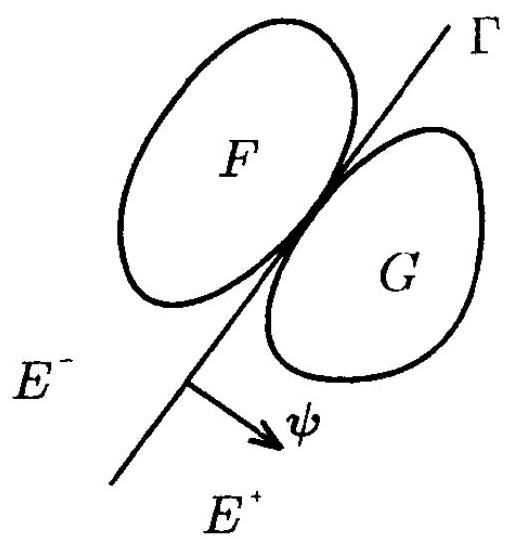
\includegraphics[max width=0.4\textwidth]{images/bo_d547okref24c73bgfch0_182_953_1589_509_545_0.jpg}
\end{center}
\hspace*{3em} 

Рис. II

где ψ — некоторый фиксированный вектор единичной длины, α — некото- рое число. Вектор ψ ортогонален ги- перплоскости Г. Если теперь множес- тва \(F,G \subset  {E}^{n}\) отделимы и гиперплос- кость \(\Gamma\) отделяет множества \(F\) и \(G\) , то будем для определенности считать, что направление вектора ψ выбрано таким образом, что множество \(F\) содержится в отрицательном полупространстве относительно вектора \(\psi\) , a множество \(G\) — в положительном. (В противном случае заменим вектор \(\psi\) на - \(\psi\) .)

В этом случае для любого вектора f ∈ F выполняется нера- венство \(\langle \mathbf{f},\mathbf{\psi }\rangle  \leq  \alpha\) , a для любого вектора \(\mathbf{g} \in  G -\) неравенство \(\langle \mathbf{g},\mathbf{\psi }\rangle  \geq  \alpha\) . Вычитая одно неравенство из другого, получаем соотношение

\[
\langle \mathbf{f},\psi \rangle  - \langle \mathbf{g},\psi \rangle  \leq  0.
\]
 (Д.5)

Таким образом, если множества F и G отделимы, то существует вектор \(\psi  \in  S\) такой,что для любых векторов \(f \in  F,g \in  G\) выполняется неравенство (Д.5).

Пусть теперь неравенство (Д.5) выполнено для любых век- торов \(f \in  F,g \in  G\) . Тогда имеем соотношение

\[
\mathop{\sup }\limits_{{f \in  F}}\langle f,\psi \rangle  \leq  \mathop{\inf }\limits_{{g \in  G}}\langle g,\psi \rangle .
\]

Положим для определенности, что

\[
\alpha  = \mathop{\sup }\limits_{{f \in  F}}\langle f,\psi \rangle
\]

Тогда для любого вектора f ∈ F выполняется неравенство \(\langle \mathbf{f},\mathbf{\psi }\rangle  \leq  \alpha\) и для любого вектора g ∈ G — неравенство \(\alpha  \leq  \langle \mathbf{g},\mathbf{\psi }\rangle\) , т.е. гиперплоскость \(\langle \mathbf{x},\mathbf{\psi }\rangle  = \alpha\) отделяет множества \(F\) и \(G\) .

Таким образом, множества F и G отделимы тогда и только тогда, когда существует вектор \(\psi  \in  S\) такой,что для любых векторов \(f \in  F,g \in  G\) выполняется соотноппение (II.5).

Будем говорить, что множества F, G C C cmpozo omделимы, если существует число \(\varepsilon  > 0\) TAKOE, ЧТО МНОЖЕСТВА \({F}^{\prime } = F + {S}_{\varepsilon }\left( \mathbf{0}\right) \mathbf{u} \; {G}^{\prime } = G + {S}_{\varepsilon }\left( \mathbf{0}\right)\) or \(g\) лимы (рис. 112). Из это- ro определения и соотно- meния (Д.5) сразу следу- ет,что множества F и G строго отделимы тогда и только тогда, когда су- шествуют число ε > 0 и bektop \(\psi  \in  S\) takine,что неравенство

\[
\left\langle  {{\mathbf{f}}^{\prime },\psi }\right\rangle   - \left\langle  {{\mathbf{g}}^{\prime },\psi }\right\rangle   \leq  0
\]

\begin{center}
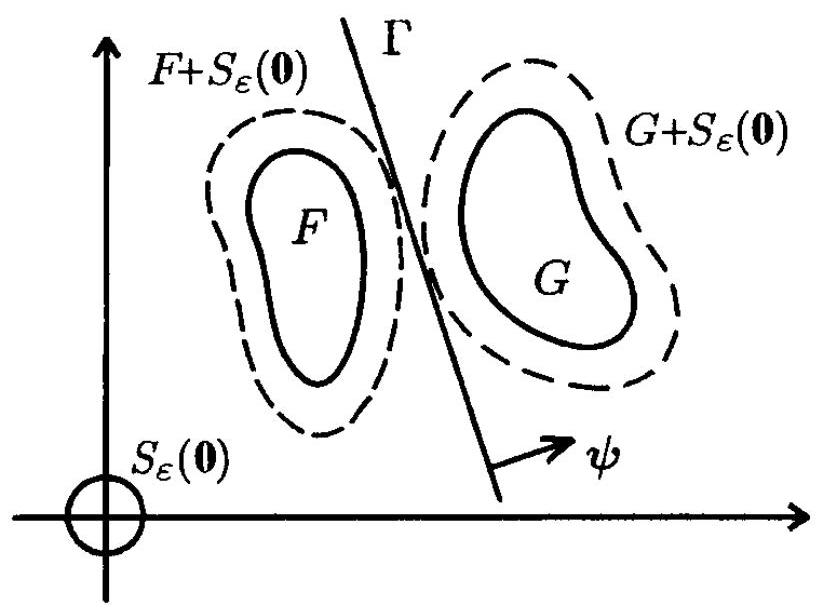
\includegraphics[max width=0.7\textwidth]{images/bo_d547okref24c73bgfch0_183_0_1514_820_613_0.jpg}
\end{center}
\hspace*{3em} 

Pnc. Д2

выполняется для любых векторов

\[
{\mathbf{f}}^{\prime } \in  F + {S}_{\varepsilon }\left( \mathbf{0}\right) ,\;{\mathbf{g}}^{\prime } \in  G + {S}_{\varepsilon }\left( \mathbf{0}\right) .
\]

Так как по определению суммы множеств векторы \({\mathbf{f}}^{\prime }\) и \({\mathbf{g}}^{\prime }\) пред- ставимы в виде

\[
{\mathbf{f}}^{\prime } = \mathbf{f} + \mathbf{u},\;{\mathbf{g}}^{\prime } = \mathbf{g} + \mathbf{v},\;\mathbf{f} \in  F,\;\mathbf{g} \in  G,\;\mathbf{u},\mathbf{v} \in  {S}_{\varepsilon }\left( \mathbf{0}\right) ,
\]

то выполнение полученного неравенства эквивалентно выпол- нению неравенства

\[
\langle \mathbf{f},\mathbf{\psi }\rangle  - \langle \mathbf{g},\mathbf{\psi }\rangle  + \langle \mathbf{u},\mathbf{\psi }\rangle  - \langle \mathbf{v},\mathbf{\psi }\rangle  \leq  0
\]
 (Д.6)

для любых векторов

\[
\mathbf{f} \in  F,\;\mathbf{g} \in  G,\;\mathbf{u},\mathbf{v} \in  {S}_{\varepsilon }\left( \mathbf{0}\right) .
\]

Покажем, что выполнение этого неравенства в свою очередь эквивалентно выполнению неравенства

\[
\langle \mathbf{f},\psi \rangle  - \langle \mathbf{g},\psi \rangle  + {2\varepsilon } \leq  0
\]
 (Д.7)

для любых векторов \(f \in  F,g \in  G\) .

Действительно, пусть неравенство (Д.6) выполняется для любых векторов

\[
\mathbf{f} \in  F,\;\mathbf{g} \in  G,\;\mathbf{u},\mathbf{v} \in  {S}_{\varepsilon }\left( \mathbf{0}\right) .
\]

Положим \(\mathbf{u} = \varepsilon \mathbf{\psi }\) и \(\mathbf{v} =  - \varepsilon \mathbf{\psi }\) . Тогда

\[
\langle \mathbf{u},\mathbf{\psi }\rangle  - \langle \mathbf{v},\mathbf{\psi }\rangle  = \varepsilon \parallel \mathbf{\psi }\parallel  + \varepsilon \parallel \mathbf{\psi }\parallel  = {2\varepsilon }
\]

и из соотношения (II.6) следует неравенство (II.7).

Для любых векторов \(u \in  {S}_{\varepsilon }\left( 0\right) , - v \in  {S}_{\varepsilon }\left( 0\right)\) и \(\psi  \in  S\) имеем

\[
\langle \mathbf{u},\mathbf{\psi }\rangle  \leq  \parallel \mathbf{u}\parallel  \cdot  \parallel \mathbf{\psi }\parallel  \leq  \varepsilon ,\;\langle  - \mathbf{v},\mathbf{\psi }\rangle  \leq  \parallel  - \mathbf{v}\parallel  \cdot  \parallel \mathbf{\psi }\parallel  \leq  \varepsilon ,
\]

следовательно, \(- {2\varepsilon } \leq   - \langle \mathbf{u},\mathbf{\psi }\rangle  + \langle \mathbf{v},\mathbf{\psi }\rangle\) . Пусть теперь выполняет- ся неравенство (Д.7). Тогда, учитывая последнее неравенство, приходим к соотношению

\[
\langle \mathbf{f},\psi \rangle  - \langle \mathbf{g},\psi \rangle  \leq   - {2\varepsilon } \leq   - \langle \mathbf{u},\psi \rangle  + \langle \mathbf{v},\psi \rangle ,
\]

т.е. получаем неравенство (Д.6).

Итак, доказано, что множества F, G C E \({}^{n}\) строго отделимы тогда и только тогда, когда существуют число ε > 0 и вектор \(\mathbf{\psi } \in  S\) такие, что неравенство (II.7) выполняется для любых векторов \(f \in  F,g \in  G\) . Заметим, что из строгой отделимости двух множеств следует их отделимость.

Пусть множества \(F\) и \(G\) непустые и компактные,т.е. \(F,G \in \; \in  \Omega \left( {E}^{n}\right)\) . B этом случае из соотнопения \(\left( {\text{ Д. }5}\right)\) получаем

\[
c\left( {F,\psi }\right)  + c\left( {G, - \psi }\right)  = \mathop{\max }\limits_{{f \in  F}}\langle f,\psi \rangle  + \mathop{\max }\limits_{{g \in  G}}\langle g, - \psi \rangle  \leq  0.
\]

Это означает, что множества F, G ∈ Ω(E') отделимы тогда и только тогда, когда существует вектор \(\psi  \in  S\) такой,что вы- полняется неравенство

\[
c\left( {F,\psi }\right)  + c\left( {G, - \psi }\right)  \leq  0. \tag{II.8}
\]

Аналогично из неравенства (II.7) следует, что

\[
c\left( {F,\psi }\right)  + c\left( {G, - \psi }\right)  + {2\varepsilon } = \mathop{\max }\limits_{{f \in  F}}\langle f,\psi \rangle  + \mathop{\max }\limits_{{g \in  G}}\langle g, - \psi \rangle  + {2\varepsilon } \leq  0,
\]

т.е. множества \(F,G \in  \Omega \left( {E}^{n}\right)\) crporo отделимы тогда и только тогда, когда существуют число ε > 0 и вектор ψ ∈ S такие, что выполняется неравенство

\[
c\left( {F,\psi }\right)  + c\left( {G, - \psi }\right)  + {2\varepsilon } \leq  0.
\]
 (Д.9)

Докажем две леммы об отделимости и строгой отделимости точки от множества.

Лемма о строгой отделимости. Пусть множество F C C \({E}^{n}\) замкнуто и выпукло, а точка g ∈ E" не принадлежит множеству F. Тогда множества F и \{g\} строго отделимы.

Доказательство. Пусть F — замкнутое выпуклое мно- жество и \(g \notin  F\) . Oпределим расстояние \(\rho \left( {g,F}\right)\) or точки \(g\) до множества \(F\) формулой

\[
\rho \left( {g,F}\right)  = \mathop{\min }\limits_{{f \in  F}}\parallel g - f\parallel .
\]

Hopma \(\parallel \mathbf{g} - \mathbf{f}\parallel\) ectb функция непрерывная, а множество F за- мкнуто. Следовательно, минимум функции [|g-f|| достигается на некотором векторе \({\mathbf{f}}_{0} \in  F\) (рис. Д3). Так как \(\mathbf{g} \notin  F\) ,имеем

\[
\rho \left( {\mathbf{g},F}\right)  = \left\lVert \begin{array}{c} {\mathbf{g} - {\mathbf{f}}_{0}} \end{array} \right\rVert > 0.
\]
 (Д.10)

\begin{center}
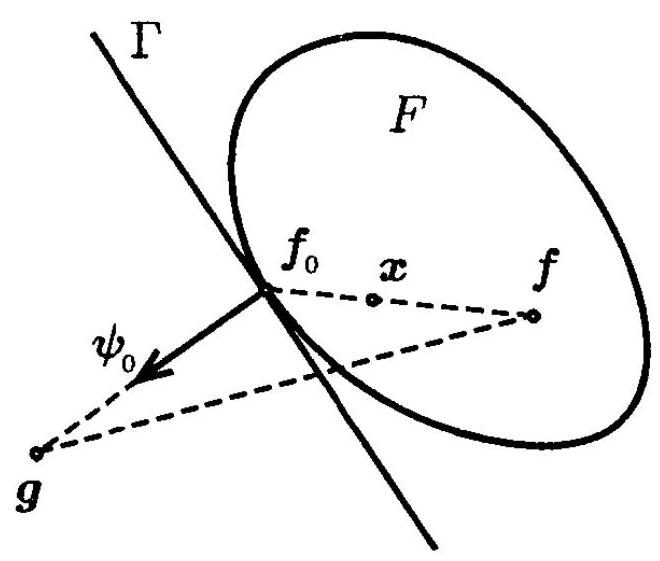
\includegraphics[max width=0.6\textwidth]{images/bo_d547okref24c73bgfch0_186_795_6_660_561_0.jpg}
\end{center}
\hspace*{3em} 

Pnc. Д3

Более того, для любого вектора \(f \in  F\) выполняется неравенство

\[
\parallel \mathbf{f} - \mathbf{g}\parallel  \geq  \left\lVert \begin{array}{c} {{\mathbf{f}}_{0} - \mathbf{g}} \end{array} \right\rVert.
\]
 (Д.11)

Зафиксируем некоторый век- тор \(f \in  F\) и соединим его от- резком с точкой \({f}_{0}\) . Произволь- ную точку этого отрезка запишем в виде

\[
\mathbf{x} = \lambda \mathbf{f} + \left( {1 - \lambda }\right) {\mathbf{f}}_{0} = {\mathbf{f}}_{0} + \lambda \left( {\mathbf{f} - {\mathbf{f}}_{0}}\right) ,
\]

где число λ выбираем из отрез- ка \(\left\lbrack  {0,1}\right\rbrack\) . Так как множество F выпукло, то х ∈ F для всех \(0 \leq  \lambda  \leq  1\) . Применяя к точке х € F соотнопение (Д.11), полу- чаем неравенство

\[
\parallel \mathbf{x} - \mathbf{g}\parallel  \geq  \left\lVert \begin{array}{c} {{\mathbf{f}}_{0} - \mathbf{g}} \end{array} \right\rVert,
\]

следовательно,

\[
\langle \mathbf{x} - \mathbf{g},\mathbf{x} - \mathbf{g}\rangle  = \parallel \mathbf{x} - \mathbf{g}{\parallel }^{2} \geq  {\left\lVert \begin{array}{c} {\mathbf{f}}_{0} - \mathbf{g} \end{array} \right\rVert}^{2}.
\]

Подставляя Вместо \(\mathbf{x}\) еговыражение через \(\lambda\) ,имеем

\[
\left\langle  {{\mathbf{f}}_{0} + \lambda \left( {\mathbf{f} - {\mathbf{f}}_{0}}\right)  - \mathbf{g},{\mathbf{f}}_{0} + \lambda \left( {\mathbf{f} - {\mathbf{f}}_{0}}\right)  - \mathbf{g}}\right\rangle   \geq  {\left\lVert \begin{array}{c} {\mathbf{f}}_{0} - \mathbf{g} \end{array} \right\rVert}^{2},
\]

т.е.для всех \(0 \leq  \lambda  \leq  1\) выполняется неравенство

\[
{\left\lVert \begin{array}{c} \mathbf{f} - {\mathbf{f}}_{0} \end{array} \right\rVert}^{2}{\lambda }^{2} + 2\left\langle  {\mathbf{f} - {\mathbf{f}}_{0},{\mathbf{f}}_{0} - \mathbf{g}}\right\rangle  \lambda  \geq  0.
\]

Обозначим левую часть этого неравенства через \(\varphi \left( \lambda \right)\) . Тогда \(\varphi \left( \lambda \right)  \geq  0\) при \(0 \leq  \lambda  \leq  1\) и \(\varphi \left( 0\right)  = 0\) . Следовательно, \({\varphi }^{\prime }\left( 0\right)  \geq  0\) , т.е. \(\left\langle  {\mathbf{f} - {\mathbf{f}}_{0},{\mathbf{f}}_{0} - \mathbf{g}}\right\rangle   \geq  0\) . Поскольку вектор \(\mathbf{f} \in  F\) был выбран произвольно, неравенство

\[
\left\langle  {\mathbf{f} - {\mathbf{f}}_{0},{\mathbf{f}}_{0} - \mathbf{g}}\right\rangle   \geq  0
\]
 (Д.12)

выполняется для любого вектора f ∈ F.

Tak как по условию (II.10) \(\left\lVert \begin{array}{c} {\mathbf{g} - {\mathbf{f}}_{0}} \end{array} \right\rVert \neq  0\) , to paccмотрим вектор \({\mathbf{\psi }}_{0} = \frac{\mathbf{g} - {\mathbf{f}}_{0}}{\left\lVert \begin{array}{c} \mathbf{g} - {\mathbf{f}}_{0} \end{array} \right\rVert}\) . Проверим для этого вектора фо соотноше- ние (Д.7). Учитывая неравенство (Д.12), получим

\[
\left\langle  {\mathbf{f},{\mathbf{\psi }}_{0}}\right\rangle   - \left\langle  {\mathbf{g},{\mathbf{\psi }}_{0}}\right\rangle   = \frac{\left\langle  {\mathbf{f},\mathbf{g} - {\mathbf{f}}_{0}}\right\rangle   - \left\langle  {\mathbf{g},\mathbf{g} - {\mathbf{f}}_{0}}\right\rangle  }{\left\lVert \begin{array}{c} \mathbf{g} - {\mathbf{f}}_{0} \end{array} \right\rVert} \leq
\]

\[
\leq  \frac{\left\langle  {\mathbf{f}}_{0},\mathbf{g} - {\mathbf{f}}_{0}\right\rangle  }{\left\lVert \begin{array}{c} \mathbf{g} - {\mathbf{f}}_{0} \end{array} \right\rVert} - \frac{\left\langle  \mathbf{g},\mathbf{g} - {\mathbf{f}}_{0}\right\rangle  }{\left\lVert \begin{array}{c} \mathbf{g} - {\mathbf{f}}_{0} \end{array} \right\rVert} =  - \left\lVert \begin{array}{c} {\mathbf{g} - {\mathbf{f}}_{0}} \end{array} \right\rVert.
\]

Если положить \({2\varepsilon } = \left\lVert \begin{array}{c} {\mathbf{g} - {\mathbf{f}}_{0}} \end{array} \right\rVert > 0\) ,то неравенство (Д.7) будет выполняться для любого вектора f ∈ F. Cледовательно, мно- жества \(F\) и \(\{ g\}\) строго отделимы и лемма доказана.

Следствие. Пусть множество F ∈ Ω(E") выпукло, а точ- \({\kappa a}\mathbf{g} \in  {E}^{n}\) не принадлежит множеству F. Тогда существует вектор \(\psi  \in  S\) maкой,что выполняется строгое неравенство

\[
c\left( {F,\psi }\right)  < \langle \mathbf{g},\psi \rangle .
\]
 (Д.13)

Доказательство. В силу леммы множества F и G = \{g\} строго отделимы и, следовательно, существуют число ε > 0 и вектор \(\psi  \in  S\) такие,что выполняется неравенство (Д.10),т.е.

\[
c\left( {F,\psi }\right)  + \langle \mathbf{g}, - \psi \rangle  + {2\varepsilon } \leq  0.
\]

Поскольку \(\varepsilon  > 0\) , из этого неравенства следует неравенство (Д.13) и следствие доказано.

На рис. Д3 ясно виден геометрический смысл неравенст- ва (П.13).

Лемма об отделимости. Пусть множество F C Е" за- мкнуто и выпукло, а точка g ∈ Е" не принадлежит внутрен- ности множества F. Тогда множества F и \{g\} отделимы.

Доказательство. Поскольку \(g \notin  \operatorname{int}F\) , cyществует такая последовательность точек \{g\}, не принадлежащих множеству \(F\) , которая сходится к точке g. Согласно лемме о строгой отде- лимости каждая точка \({\mathbf{g}}_{k}\) строго отделима от множества F, сле- довательно, просто отделима. Тогда существует вектор \({\mathbf{\psi }}_{k} \in  S\) такой, что для любого вектора f ∈ F выполняется неравенство (Д.5), т.е.

\[
\left\langle  {\mathbf{f},{\psi }_{k}}\right\rangle   - \left\langle  {{\mathbf{g}}_{k},{\psi }_{k}}\right\rangle   \leq  0.
\]
 (Д.14)

Поскольку единичная сфера S есть множество компактное, из последовательности \(\left\{  {\mathbf{\psi }}_{k}\right\}\) можно выделить подпоследователь- ность, сходящуюся к некоторой точке ψ ∈ S. Обозначим эту подпоследовательность снова через \{ \({\psi }_{k}\) \}. Тогда для любого век- тора f ∈ F, используя предельный переход в неравенстве (II.14), получаем

\[
\langle f,\psi \rangle  - \langle g,\psi \rangle  \leq  0,
\]

т.е. для вектора ф выполняется соотношение (Д.5). Следова- тельно, множества F и \{g\} отделимы и лемма доказана.

Следствие. Пусть множество F ∈ Ω(Ег″ выпукло и точ- \({\kappa a}{\mathbf{f}}_{0}\) принадлежит границе множества F, т.е. \({\mathbf{f}}_{0} \in  \partial F\) . Tor- да существует вектор \({\mathbf{\psi }}_{0} \in  S\) ,который является опорным к множеству \(F\) в точке \({\mathbf{f}}_{0}\) (см. рис. Д3).

Доказательство. Поскольку точка \({\mathbf{f}}_{0}\) не принадлежит внутренности множества F, по лемме об отделимости множест- ва F и G = \(\left\{  {\mathbf{f}}_{0}\right\}\) отделимы. Следовательно, существует вектор \({\psi }_{0} \in  S\) такой,что выполняется неравенство (Д.8),т.е.

\[
c\left( {F,{\psi }_{0}}\right)  + \left\langle  {{\mathbf{f}}_{0}, - {\psi }_{0}}\right\rangle   \leq  0.
\]

Согласно следствию из свойства 6 опорных функций (см. лек- цию 3), из включения \({\mathbf{f}}_{0} \in  F\) следует неравенство

\[
\left\langle  {{\mathbf{f}}_{0},\psi }\right\rangle   \leq  c\left( {F,{\psi }_{0}}\right) .
\]

Из двух последних неравенств вытекает равенство

\[
c\left( {F,{\psi }_{0}}\right)  = \left\langle  {{\mathbf{f}}_{0},{\psi }_{0}}\right\rangle  .
\]

Таким образом, вектор \({\mathbf{\psi }}_{0}\) является опорным к множеству \(F\) в точке \({\mathbf{f}}_{0}\) .

Теорема o crporoй отделимости. Два выпуклых мно- жества F, G ∈ Ω( \(\bar{{E}^{n}}\) ) cmpozo отделимы тогда и только тог- \(\partial a,\kappa\) or \(\partial a\) они не пересекаются, т.е. \(\kappa\) or \(\partial aF \cap  G = \varnothing\) .

Доказательство. Два множества \(F,G \in  \Omega \left( {E}^{n}\right)\) строго отделимы тогда и только тогда, когда существуют число ε > 0 и вектор \(\psi  \in  S\) такие, что выполняется неравенство (П.9), т.е. для этого вектора ψ с 8 выполняется неравенство

\[
c\left( {F,\psi }\right)  + c\left( {G, - \psi }\right)  < 0.
\]

Согласно свойству 12 опорных функций (см. лекцию 3) два выпуклых множества \(F,G \in  \Omega \left( {E}^{n}\right)\) пересекаются тогда и толь- ко тогда, когда для всех векторов \(\psi  \in  S\) выполняется неравен- CTBO

\[
c\left( {F,\psi }\right)  + c\left( {G, - \psi }\right)  \geq  0.
\]

Отсюда сразу следует утверждение теоремы. Теорема доказана.

Теорема об отделимости. Два выпуклых множества \(F,G \in  \Omega \left( {E}^{n}\right)\) omделимы тогда и только тогда, когда

\[
0 \notin  \operatorname{int}\left\lbrack  {F + \left( {-1}\right) G}\right\rbrack \tag{II.15}
\]

Доказательство. Два множества F, G ∈ Ω(E \({}^{n}\) ) отделимы тогда и только тогда, когда существует вектор \(\psi  \in  S\) такой,что выполняется неравенство (Д.8).

C другой стороны, множество F+ (−1)G выпукло, и соглас- но следствию из свойства 14 опорных функций (см. лекцию 3) соотношее (Д.15) выполняется тогдаи только тогла, когда

\[
0 < c\left( {F,\psi }\right)  + c\left( {G, - \psi }\right)
\]

для любого вектора фе S. Отсюда сразу следует утверждение теоремы. Теорема доказана.

Заметим, что если внутренность множества F+ (−1)G пус- та, то выпуклые множества \(F,G \in  \Omega \left( {E}^{n}\right)\) всегда отделимы.

\section*{ДЗ. Выпуклые функции}

Функция f : \({E}^{n} \rightarrow  {E}^{1}\) называется выпуклой (см. лек- цию 3), если для любых двух точек х, и, хе сей сли любого числа \(0 \leq  \lambda  \leq  1\) выполняется неравенство

\[
f\left( {\lambda {\mathbf{x}}_{1} + \left( {1 - \lambda }\right) {\mathbf{x}}_{2}}\right)  \leq  {\lambda f}\left( {\mathbf{x}}_{1}\right)  + \left( {1 - \lambda }\right) f\left( {\mathbf{x}}_{2}\right) .
\]
 (Д.16)

По индукции легко показать, что для любой выпуклой комби- нации

\[
\mathbf{x} = {\lambda }_{1}{\mathbf{x}}_{1} + \ldots  + {\lambda }_{m}{\mathbf{x}}_{m},\;{\mathbf{x}}_{1},\ldots ,{\mathbf{x}}_{m} \in  {E}^{n},\;{\lambda }_{i} \geq  0,
\]

\[
{\lambda }_{1} + \ldots  + {\lambda }_{m} = 1
\]

выпуклая функция \(f\left( x\right)\) удовлетворяет неравенству

\[
f\left( {{\lambda }_{1}{\mathbf{x}}_{1} + \ldots  + {\lambda }_{m}{\mathbf{x}}_{m}}\right)  \leq  {\lambda }_{1}f\left( {\mathbf{x}}_{1}\right)  + \ldots  + {\lambda }_{m}f\left( {\mathbf{x}}_{m}\right) .
\]
 (Д.17)

Читателю предлагается сделать это самостоятельно.

Примеры выпуклых функций были рассмотрены в лекции 3. Именно, для любого множества F ∈ \(\Omega \left( {E}^{n}\right)\) ero опорная функ- ция \(c\left( {F,\mathbf{\psi }}\right)\) является функцией, выпуклой по аргументу ψ ∈ \({E}^{n}\) (следствие из свойств 1 и 2). В лекции 3 показано, что опорная функция \(c\left( {F,\psi }\right)\) для множества \(F \in  \Omega \left( {E}^{n}\right)\) является функцией, непрерывной по \(\mathbf{\psi }\) (следствие из свойства 13). Оказывается, лю- бая выпуклая функция, если она принимает конечные значения, т.е. \(f\left( \mathbf{x}\right)  \neq  \infty\) ,является функцией непрерывной.

Теорема 1. Ecлu функция \(f : {E}^{n} \rightarrow  {E}^{1}\) выпукла и конечна, то она непрерывна.

Доказательство. Зафиксируем произвольную точку х, с \(\in  {E}^{n}\) и рассмотрим близкую к ней точку х а с. если слесмотрим базисные векторы \({e}_{1},\ldots ,{e}_{n}\) в пространстве E" и противопо- ложные им векторы \({e}_{n + 1} =  - {e}_{1},\ldots ,{e}_{2n} =  - {e}_{n}\) . Вектор прира- щения аргумента Δx = (Δx',…, Δx’) разложим по векторам \({e}_{1},\ldots ,{e}_{2n}\) , т.е. представим в виде

\[
{\Delta x} = {\xi }_{1}{e}_{1} + \ldots  + {\xi }_{2n}{e}_{2n}
\]
 (Д.18)

следующим образом: если \(\Delta {x}^{i} \geq  0\) , то положим \({\xi }_{i} = \Delta {x}^{i}\) , \({\xi }_{n + i} = 0\) , ecли \(\Delta {x}^{i} < 0\) , to положим \({\xi }_{i} = 0,{\xi }_{n + i} =  - \Delta {x}^{i}\) . Таким образом, в этом представлении все числа б, неотрицательны, т.е. \({\xi }_{i} \geq  0\) и \({\xi }_{i} \leq  \parallel \mathbf{{\Delta x}}\parallel\) . Будем считать, что вектор Δx достаточно мал, так что \({\xi }_{i} \leq  1,i = 1,\ldots ,{2n}\) . Согласно формулам (A.17) и (A.16) имеем

\[
f\left( {{\mathbf{x}}_{0} + \mathbf{\Delta }\mathbf{x}}\right)  = f\left( {{\mathbf{x}}_{0} + \mathop{\sum }\limits_{{i = 1}}^{{2n}}{\xi }_{i}{\mathbf{e}}_{i}}\right)  = f\left( {\frac{1}{2n}\mathop{\sum }\limits_{{i = 1}}^{{2n}}\left( {{\mathbf{x}}_{0} + {\xi }_{i}{2n}{\mathbf{e}}_{i}}\right) }\right)  \leq
\]

\[
\leq  \frac{1}{2n}\mathop{\sum }\limits_{{i = 1}}^{{2n}}f\left( {{\mathbf{x}}_{0} + {\xi }_{i}{2n}{\mathbf{e}}_{i}}\right)  = \frac{1}{2n}\mathop{\sum }\limits_{{i = 1}}^{{2n}}f\left\lbrack  {\left( {1 - {\xi }_{i}}\right) {\mathbf{x}}_{0} + {\xi }_{i}\left( {{\mathbf{x}}_{0} + {2n}{\mathbf{e}}_{i}}\right) }\right\rbrack   \leq
\]

\[
\leq  \frac{1}{2n}\mathop{\sum }\limits_{{i = 1}}^{{2n}}\left\lbrack  {\left( {1 - {\xi }_{i}}\right) f\left( {\mathbf{x}}_{0}\right)  + {\xi }_{i}f\left( {{\mathbf{x}}_{0} + {2n}{\mathbf{e}}_{i}}\right) }\right\rbrack  .
\]

Оценим теперь приращение функции. Используя полученное неравенство, получаем

\[
f\left( {{x}_{0} + {\Delta x}}\right)  - f\left( {x}_{0}\right)  \leq
\]

\[
\leq  \frac{1}{2n}\mathop{\sum }\limits_{{i = 1}}^{{2n}}\left\lbrack  {\left( {1 - {\xi }_{i}}\right) f\left( {x}_{0}\right)  + {\xi }_{i}f\left( {{x}_{0} + {2n}{e}_{i}}\right) }\right\rbrack   - f\left( {x}_{0}\right)  =
\]

\[
= \frac{1}{2n}\mathop{\sum }\limits_{{i = 1}}^{{2n}}{\xi }_{i}\left\lbrack  {f\left( {{x}_{0} + {2n}{e}_{i}}\right)  - f\left( {x}_{0}\right) }\right\rbrack  .
\]

Поскольку функция \(f\left( \mathbf{x}\right)  \neq  \infty\) ,то все выражения в квадрат- ных скобках есть некоторые числа, поэтому правая часть этого неравенства стремится к нулю, когда Δx → 0. Следовательно, для любого числа \(\varepsilon  > 0\) cyществует число δ > 0 такое, что для любого приращения \(\mathbf{{\Delta x}} \in  {E}^{n}\) выполняется неравенство

\[
f\left( {{\mathbf{x}}_{0} + \Delta \mathbf{x}}\right)  - f\left( {\mathbf{x}}_{0}\right)  \leq  \varepsilon ,
\]
 (Д.19)

как только || \({\Delta x} \parallel   < \delta\) . Пусть || \({\Delta x} \parallel   < \delta\) . Используя снова фор- мулу (Д.16), получим

\[
f\left( {\mathbf{x}}_{0}\right)  = f\left( {\frac{{\mathbf{x}}_{0} + \Delta \mathbf{x}}{2} + \frac{{\mathbf{x}}_{0} - \Delta \mathbf{x}}{2}}\right)  \leq
\]

\[
\leq  \frac{1}{2}f\left( {{\mathbf{x}}_{0} + \Delta \mathbf{x}}\right)  + \frac{1}{2}f\left( {{\mathbf{x}}_{0} - \Delta \mathbf{x}}\right) ,
\]

т.е. \(f\left( {\mathbf{x}}_{0}\right)  - f\left( {{\mathbf{x}}_{0} + \mathbf{{\Delta x}}}\right)  < f\left( {{\mathbf{x}}_{0} - \mathbf{{\Delta x}}}\right)  - f\left( {\mathbf{x}}_{0}\right)\) . Правая часть этого неравенства меньше б в силу формулы (Д.19), так как \(\parallel  - \mathbf{\Delta }\mathbf{x}\parallel  \leq  \delta\) , noэтому \(f\left( {\mathbf{x}}_{0}\right)  - f\left( {{\mathbf{x}}_{0} + \mathbf{\Delta }\mathbf{x}}\right)  \leq  \varepsilon\) . Сравнивая полу- ченное неравенство с формулой (Д.19), получаем соотношение

\[
\left| {f\left( {{x}_{0} + {\Delta x}}\right)  - f\left( {x}_{0}\right) }\right|  \leq  \varepsilon
\]

при достаточно малых приращениях Δx.

Таким образом, функция \(f\left( \mathbf{x}\right)\) непрерывна в точке \({\mathbf{x}}_{0}\) и тео- рема 1 доказана.

Рассмотрим вновь произвольную функцию \(f : {E}^{n} \rightarrow  {E}^{1}\) и некоторый вектор \(h \in  {E}^{n}\) . Производной \({f}^{\prime }\left( {\mathbf{x};\mathbf{h}}\right)\) om \({\phi y}\# {\kappa u\mu u} \; f\left( \mathbf{x}\right)\) в точке х по направлению h называется предел функции

\[
\varphi \left( \alpha \right)  = \frac{f\left( {\mathbf{x} + \alpha \mathbf{h}}\right)  - f\left( \mathbf{x}\right) }{\alpha }
\]

при положительных α, стремящихся к нулю, если, конечно, он существует. Таким образом,

\[
{f}^{\prime }\left( {\mathbf{x};\mathbf{h}}\right)  = \mathop{\lim }\limits_{{\alpha  \rightarrow   + 0}}\varphi \left( \alpha \right)  = \mathop{\lim }\limits_{{\alpha  \rightarrow   + 0}}\frac{f\left( {\mathbf{x} + \alpha \mathbf{h}}\right)  - f\left( \mathbf{x}\right) }{\alpha }.
\]
 (Д.20)

Теорема 2. Ecau функция \(f : {E}^{n} \rightarrow  {E}^{1}\) выпукла и конечна, то в любой точке х ∈ \({E}^{n}u\) для любого направления h ∈ \({E}^{n}\) функция \(\varphi \left( \alpha \right)  = \frac{f\left( {x + {\alpha h}}\right)  - f\left( x\right) }{\alpha }\) не возрастает при а → +0 и ограничена снизу. Таким образом, в любой точке хе Ег про- изводная \({f}^{\prime }\left( {\mathbf{x};\mathbf{h}}\right)\) no любому направлению \(\mathbf{h} \in  {E}^{n}\) cyu.ecm.pyem. Более того, производная по направлению удовлетворяет сле- дующим свойствам:

1) \({f}^{\prime }\left( {\mathbf{x};\lambda \mathbf{h}}\right)  = \lambda {f}^{\prime }\left( {\mathbf{x};\mathbf{h}}\right) \;\forall \lambda  \geq  0\) ;

2) \({f}^{\prime }\left( {\mathbf{x};{\mathbf{h}}_{1} + {\mathbf{h}}_{2}}\right)  \leq  {f}^{\prime }\left( {\mathbf{x};{\mathbf{h}}_{1}}\right)  + {f}^{\prime }\left( {\mathbf{x};{\mathbf{h}}_{2}}\right) \;\forall {\mathbf{h}}_{1},{\mathbf{h}}_{2} \in  {E}^{n}\) .

Доказательство. Зафиксируем векторы х, н ∈ E". Если мы покажем, что функция \(\varphi \left( \alpha \right)\) при \(\alpha  \rightarrow  0\) не возрастает и огра- ничена снизу, то предел в соотношении (Д.20) будет существо- вать и будет конечен, т.е. мы докажем тогда, что производная \({f}^{\prime }\left( {\mathbf{x};\mathbf{h}}\right)\) cyществует.

Пусть числа \({\alpha }_{1},{\alpha }_{2}\) таковы,что \({\alpha }_{1} > {\alpha }_{2} > 0\) . Положим в формуле (II. 16) \(\lambda  = \frac{{\alpha }_{2}}{{\alpha }_{1}},1 - \lambda  = \frac{{\alpha }_{1} - {\alpha }_{2}}{{\alpha }_{1}}\) и \({\mathbf{x}}_{1} = \mathbf{x} + {\alpha }_{1}\mathbf{h},{\mathbf{x}}_{2} = \mathbf{x}\) , при этом получим \(\lambda {\mathbf{x}}_{1} + \left( {1 - \lambda }\right) {\mathbf{x}}_{2} = \mathbf{x} + {\alpha }_{2}\mathbf{h}\) u

\[
f\left( {\mathbf{x} + {\alpha }_{2}\mathbf{h}}\right)  \leq  \frac{{\alpha }_{2}}{{\alpha }_{1}}f\left( {\mathbf{x} + {\alpha }_{1}\mathbf{h}}\right)  + \frac{{\alpha }_{1} - {\alpha }_{2}}{{\alpha }_{1}}f\left( \mathbf{x}\right) .
\]

Следовательно,

\[
\frac{f\left( {\mathbf{x} + {\alpha }_{2}\mathbf{h}}\right)  - f\left( \mathbf{x}\right) }{{\alpha }_{2}} \leq  \frac{1}{{\alpha }_{1}}f\left( {\mathbf{x} + {\alpha }_{1}\mathbf{h}}\right)  + \frac{{\alpha }_{1} - {\alpha }_{2}}{{\alpha }_{1}{\alpha }_{2}}f\left( \mathbf{x}\right)  - \frac{1}{{\alpha }_{2}}f\left( \mathbf{x}\right)  =
\]

\[
= \frac{f\left( {\mathbf{x} + {\alpha }_{1}\mathbf{h}}\right)  - f\left( \mathbf{x}\right) }{{\alpha }_{1}},
\]

т.е. \(\varphi \left( {\alpha }_{2}\right)  \leq  \varphi \left( {\alpha }_{1}\right)\) и функция \(\varphi \left( \alpha \right)\) не возрастает при \(\alpha  \rightarrow   + 0\) .

Положив в формуле (Д.16) \(\lambda  = \frac{1}{1 + \alpha },\;1 - \lambda  = \frac{\alpha }{1 + \alpha }\) и \({\mathbf{x}}_{1} = \mathbf{x} + \alpha \mathbf{h},{\mathbf{x}}_{2} = \mathbf{x} - \mathbf{h}\) ,получим 入 \({\mathbf{x}}_{1} + \left( {1 - \lambda }\right) {\mathbf{x}}_{2} = \mathbf{x}\) и

\[
f\left( \mathbf{x}\right)  \leq  \frac{1}{1 + \alpha }f\left( {\mathbf{x} + \alpha \mathbf{h}}\right)  + \frac{\alpha }{1 + \alpha }f\left( {\mathbf{x} - \mathbf{h}}\right) .
\]

Следовательно,

\[
\frac{f\left( {\mathbf{x} + \alpha \mathbf{h}}\right)  - f\left( \mathbf{x}\right) }{\alpha } \geq  \frac{\left( {1 + \alpha }\right) f\left( \mathbf{x}\right)  - {\alpha f}\left( {\mathbf{x} - \mathbf{h}}\right)  - f\left( \mathbf{x}\right) }{\alpha } =
\]

\[
= f\left( \mathbf{x}\right)  - f\left( {\mathbf{x} - \mathbf{h}}\right) .
\]

Поскольку функция \(f\left( \mathbf{x}\right)  \neq  0\) , то правая часть этого неравенства есть конечное число, следовательно, функция \(\varphi \left( \alpha \right)\) orраничена снизу.

Мы доказали, что предел (Д.20) существует и конечен, т.е. функция \(f\left( \mathbf{x}\right)\) в точке х дифференцируема по направлению h. Свойство 1 сразу следует из соотношения (Д.20). Действитель- но, пусть \(\lambda  > 0\) (при \(\lambda  = 0\) свойство 1,0чевидно,выполняется), тогда

\[
{f}^{\prime }\left( {\mathbf{x};\lambda \mathbf{h}}\right)  = \mathop{\lim }\limits_{{\alpha  \rightarrow   + 0}}\frac{f\left( {\mathbf{x} + {\alpha \lambda }\mathbf{h}}\right)  - f\left( \mathbf{x}\right) }{\alpha } =
\]

\[
= \lambda \mathop{\lim }\limits_{{\alpha  \rightarrow   + 0}}\frac{f\left( {\mathbf{x} + {\alpha \lambda }\mathbf{h}}\right)  - f\left( \mathbf{x}\right) }{\alpha \lambda } = \lambda {f}^{\prime }\left( {\mathbf{x};\mathbf{h}}\right) .
\]

Для доказательства свойства 2 снова воспользуемся форму- лами (Д.16) и (Д.20). Пусть н, н, н2 е в т, тогда имеем соотно- шения

\[
{f}^{\prime }\left( {\mathbf{x};{\mathbf{h}}_{1} + {\mathbf{h}}_{2}}\right)  = \mathop{\lim }\limits_{{\alpha  \rightarrow   + 0}}\frac{f\left( {\mathbf{x} + \alpha \left( {{\mathbf{h}}_{1} + {\mathbf{h}}_{2}}\right) }\right)  - f\left( \mathbf{x}\right) }{\alpha } =
\]

\[
= \mathop{\lim }\limits_{{\alpha  \rightarrow   + 0}}\frac{f\left( {\frac{x + {2\alpha }{h}_{1}}{2} + \frac{x + {2\alpha }{h}_{2}}{2}}\right)  - f\left( x\right) }{\alpha } \leq
\]

\[
\leq  \mathop{\lim }\limits_{{\alpha  \rightarrow   + 0}}\frac{f\left( {\mathbf{x} + {2\alpha }{\mathbf{h}}_{1}}\right)  - f\left( \mathbf{x}\right) }{2\alpha } + \mathop{\lim }\limits_{{\alpha  \rightarrow   + 0}}\frac{f\left( {\mathbf{x} + {2\alpha }{\mathbf{h}}_{2}}\right)  - f\left( \mathbf{x}\right) }{2\alpha } =
\]

\[
= {f}^{\prime }\left( {\mathbf{x};{\mathbf{h}}_{1}}\right)  + {f}^{\prime }\left( {\mathbf{x};{\mathbf{h}}_{2}}\right) .
\]

Теорема полностью доказана.

Следствие. Для любого множества F ∈ Ω( \({E}^{n}\) ) его опорная функция \(c\left( {F,\mathbf{\psi }}\right)\) выпукла и конечна. Следовательно, функция

\[
\varphi \left( \alpha \right)  = \frac{c\left( {F,{\psi }_{0} + {\alpha \psi }}\right)  - c\left( {F,{\psi }_{0}}\right) }{\alpha }
\]
 (Д.21)

не возрастает при а → +0 и ограничена снизу для любых \({\psi }_{0},\psi  \in  {E}^{n}\) . Таким образом, опорная функция \(c\left( {F,\psi }\right)\) диффе- ренцируема в любой точке \({\psi }_{0} \in  {E}^{n}\) no любому направлению \(\psi  \in  {E}^{n}u\) npousводная \({c}^{\prime }\left( {F,{\psi }_{0};\psi }\right) y\partial o\) влетворяет следующим свойствам:

1) \({c}^{\prime }\left( {F,{\mathbf{\psi }}_{0};\lambda \mathbf{\psi }}\right)  = \lambda {c}^{\prime }\left( {F,{\mathbf{\psi }}_{0};\mathbf{\psi }}\right) \;\forall \lambda  \geq  0\) ;

2) \({c}^{\prime }\left( {F,{\mathbf{\psi }}_{0};{\mathbf{\psi }}_{1} + {\mathbf{\psi }}_{2}}\right)  \leq  {c}^{\prime }\left( {F,{\mathbf{\psi }}_{0};{\mathbf{\psi }}_{1}}\right)  + {c}^{\prime }\left( {F,{\mathbf{\psi }}_{0};{\mathbf{\psi }}_{2}}\right) \forall {\mathbf{\psi }}_{1},{\mathbf{\psi }}_{2} \in  {E}^{n}\) .

Функция \(f : {E}^{n} \rightarrow  {E}^{1}\) называется дифференцируемой в точке \({\mathbf{x}}_{0} \in  {E}^{n}\) , ecли существует такой вектор \(\mathbf{p} \in  {E}^{n}\) ,что для любого вектора \(\mathbf{x} \in  {E}^{n}\) выполняется соотношение

\[
f\left( \mathbf{x}\right)  - f\left( {\mathbf{x}}_{0}\right)  = \left\langle  {\mathbf{p},\mathbf{x} - {\mathbf{x}}_{0}}\right\rangle   + \bar{o}\left( \left\lVert \begin{array}{c} {\mathbf{x} - {\mathbf{x}}_{0}} \end{array} \right\rVert\right) ,
\]
 (Д.22)

где величина ō(∥x - x0 \textbackslash  ) такова, что \(\frac{\sigma \left( \left\lVert \begin{array}{c} {x - {x}_{0}} \end{array} \right\rVert\right) }{\left\lVert \begin{array}{c} x - {x}_{0}\left| \right| \end{array} \right\rVert} \rightarrow  0\) при \(\left\lVert \begin{array}{c} {\mathbf{x} - {\mathbf{x}}_{0}} \end{array} \right\rVert \rightarrow  0\) . Вектор р в этом случае называется градиентом функции \(f\left( \mathbf{x}\right)\) в точке \({\mathbf{x}}_{0}\) и обозначается через дете

Если функция дифференцируема, то ее производная по лю- бому направлению h существует и имеет вид

\[
{f}^{\prime }\left( {{\mathbf{x}}_{0};\mathbf{h}}\right)  = \left\langle  {\frac{\partial f\left( {\mathbf{x}}_{0}\right) }{\partial \mathbf{x}},\mathbf{h}}\right\rangle  .
\]
 (Д.23)

Действительно, в силу соотношения (Д.22) имеем

\[
{f}^{\prime }\left( {{\mathbf{x}}_{0};\mathbf{h}}\right)  = \mathop{\lim }\limits_{{\alpha  \rightarrow   + 0}}\frac{f\left( {{\mathbf{x}}_{0} + \alpha \mathbf{h}}\right)  - f\left( {\mathbf{x}}_{0}\right) }{\alpha } =
\]

\[
= \mathop{\lim }\limits_{{\alpha  \rightarrow   + 0}}\frac{\left\langle  {\frac{\partial f\left( {\mathbf{x}}_{0}\right) }{\partial \mathbf{x}},\alpha \mathbf{h}}\right\rangle   + \bar{o}\left( {\parallel \alpha \mathbf{h}\parallel }\right) }{\alpha } = \left\langle  {\frac{\partial f\left( {\mathbf{x}}_{0}\right) }{\partial \mathbf{x}},\mathbf{h}}\right\rangle  .
\]

Пример 1. Найдем производную по направлению от функ- ции \(f\left( \mathbf{x}\right)  = \parallel \mathbf{x}\parallel\) . Эта функция выпукла и конечна. Следователь- но, согласно теореме 2 ее производная по любому направлению существует в любой точке. Известно, что эта функция \(\parallel \mathbf{x}\parallel\) диф- ференцируема всюду, кроме точки х = 0 и дете и х не и на тому при х ≠ 0 ее производная по направлению существует и в силу формулы (Д.23) имеет вид

\[
{f}^{\prime }\left( {\mathbf{x};\mathbf{h}}\right)  = \frac{\langle \mathbf{x},\mathbf{h}\rangle }{\parallel \mathbf{x}\parallel }.
\]

При х = 0 из определения производной по направлению (см. формулу (Д.20)) имеем

\[
{f}^{\prime }\left( {\mathbf{x};\mathbf{h}}\right)  = \frac{\parallel \alpha \mathbf{h}\parallel }{\alpha } = \parallel \mathbf{h}\parallel .
\]

Если функция \(f : {E}^{n} \rightarrow  {E}^{1}\) выпукла и дифференцируема в точке \({\mathbf{x}}_{0}\) , то для любого вектора х ∈ \({E}^{n}\) выполняется неравен- CTBO

\[
\left\langle  {\frac{\partial f\left( {\mathbf{x}}_{0}\right) }{\partial \mathbf{x}},\mathbf{x} - {\mathbf{x}}_{0}}\right\rangle   \leq  f\left( \mathbf{x}\right)  - f\left( {\mathbf{x}}_{0}\right) .
\]
 (Д.24)

Действительно, пусть 0 < λ < 1. Положив в формуле (Д.16) \(\lambda  = a,{x}_{1} = x;{x}_{2} = {x}_{0}\) ,имеем

\[
f\left( {\alpha \mathbf{x} + \left( {1 - \alpha }\right) {\mathbf{x}}_{0}}\right)  \leq  {\alpha f}\left( \mathbf{x}\right)  + \left( {1 - \alpha }\right) f\left( {\mathbf{x}}_{0}\right)  = f\left( {\mathbf{x}}_{0}\right)  + \alpha \left\lbrack  {f\left( \mathbf{x}\right)  - f\left( {\mathbf{x}}_{0}\right) }\right\rbrack  .
\]

Следовательно,

\[
\frac{f\left( {{\mathbf{x}}_{0} + \alpha \left( {\mathbf{x} - {\mathbf{x}}_{0}}\right) }\right)  - f\left( {\mathbf{x}}_{0}\right) }{\alpha } \leq  f\left( \mathbf{x}\right)  - f\left( {\mathbf{x}}_{0}\right) .
\]

Переходя к пределу при \(\alpha  \rightarrow   + 0\) в левой части этого нера- венства, получим в силу дифференцируемости по направлению функции \(f\left( \mathbf{x}\right)\) в точке \({\mathbf{x}}_{0}\) неравенство

\[
{f}^{\prime }\left( {{\mathbf{x}}_{0};\mathbf{x} - {\mathbf{x}}_{0}}\right)  \leq  f\left( \mathbf{x}\right)  - f\left( {\mathbf{x}}_{0}\right) ,
\]

откуда согласно формуле (Д.23) получаем неравенство (Д.24).

Пусть теперь функция \(f : {E}^{n} \rightarrow  {E}^{1}\) просто выпукла. Вектор \(\mathbf{p} \in  {E}^{n}\) назовем субградиентом функции \(f\left( \mathbf{x}\right)\) в точке \({\mathbf{x}}_{0}\) , если для любого вектора \(\mathbf{x} \in  {E}^{n}\) выполняется неравенство

\[
\left\langle  {\mathbf{p},\mathbf{x} - {\mathbf{x}}_{0}}\right\rangle   \leq  f\left( \mathbf{x}\right)  - f\left( {\mathbf{x}}_{0}\right)
\]
 (Д.25)

(сравните с формулой (Д.24)). Совокупность всех таких векто- ров p ∈ \({E}^{n}\) назовем субдифференциалом функции \(f\left( \mathbf{x}\right)\) в точке \({\mathbf{x}}_{0}\) и обозначим д \(f\left( {\mathbf{x}}_{0}\right)\) . Таким образом,

\[
\partial f\left( {\mathbf{x}}_{0}\right)  = \left\{  {\mathbf{p} : \left\langle  {\mathbf{p},\mathbf{x} - {\mathbf{x}}_{0}}\right\rangle   \leq  f\left( \mathbf{x}\right)  - f\left( {\mathbf{x}}_{0}\right) \forall \mathbf{x} \in  {E}^{n}}\right\}  .
\]

Далее, функцию \(f\left( \mathbf{x}\right)\) назовем субдифференцируемой в точ- ке \({\mathbf{x}}_{0}\) , если у нее в этой точке существует хотя бы один суб- градиент, т.е. множество \(\partial f\left( {\mathbf{x}}_{0}\right)\) непусто. Из формулы (Д.24) следует, что если выпуклая функция \(f\left( \mathbf{x}\right)\) дифференцируема в точке \({\mathbf{x}}_{0} \in  {E}^{n}\) , то она субдифференцируема в этой точке и ее градиент \(\frac{\partial f\left( {\mathbf{x}}_{0}\right) }{\partial \mathbf{x}}\) является субградиентом, т.е. \(\frac{\partial f\left( {\mathbf{x}}_{0}\right) }{\partial \mathbf{x}} \in  \partial f\left( {\mathbf{x}}_{0}\right)\) . В разделе Д4 будет показано, что в этом случае других субгради- ентов у функции \(f\left( \mathbf{x}\right)\) в точке \({\mathbf{x}}_{0}\) больше нет, т.е. в этом случае \(\frac{\partial f\left( {\mathbf{x}}_{0}\right) }{\partial \mathbf{x}} = \partial f\left( {\mathbf{x}}_{0}\right) .\)

Пример 2. Найдем субдифференциал функции \(f\left( \mathbf{x}\right)  = \parallel \mathbf{x}\parallel\) в точке \({\mathbf{x}}_{0} = \mathbf{0}\) . Неравенство (Д.25) при этом принимает вид

\[
\langle \mathbf{p},\mathbf{x}\rangle  \leq  \parallel \mathbf{x}\parallel
\]

и должно выполняться для любого вектора \(\mathbf{x} \in  {E}^{n}\) . Ясно, что для любого вектора \(\mathbf{p}\) такого, что \(\parallel \mathbf{p}\parallel  \leq  1\) , это неравенство выполняется при всех \(\mathbf{x} \in  {E}^{n}\) , а если \(\parallel \mathbf{p}\parallel  > 1\) , то, напри- мер, для вектора \(\mathbf{x} = \frac{\mathbf{p}}{2}\) это неравенство нарушается, так как \(\frac{1}{2}\parallel \mathbf{p}{\parallel }^{2} > \frac{1}{2}\parallel \mathbf{p}\parallel\) . Следовательно, функция \(f\left( \mathbf{x}\right)  = \parallel \mathbf{x}\parallel\) субдиффе- ренцируема в точке \({\mathbf{x}}_{0} = \mathbf{0}\) и ее субдифференциал в этой точке совпадает с единичным шаром, т.е. \(\partial f\left( \mathbf{0}\right)  = {S}_{1}\left( \mathbf{0}\right)\) . Отметим, что функция \(f\left( \mathbf{x}\right)  = \parallel \mathbf{x}\parallel\) недифференцируема в точке \({\mathbf{x}}_{0} = \mathbf{0}\) . Заметим, что, вообще говоря, не любая выпуклая функция яв- ляется субдифференцируемой. Например, функция

\[
f\left( \mathbf{x}\right)  = \left\{  \begin{array}{ll}  - \sqrt{1 - \parallel \mathbf{x}\parallel }, & \text{ если }\parallel \mathbf{x}\parallel  \leq  1, \\   + \infty , & \text{ если }\parallel \mathbf{x}\parallel  > 1 \end{array}\right.
\]

не является субдифференцируемой в тех точках х ∈ E", где \(\parallel \mathbf{x}\parallel  > 1\) . Читателю предлагается проверить этот факт самосто- ятельно.

\section*{Задачи}

1. Докажите, что функция \(f\left( x\right)  = \mathop{\max }\limits_{{1 \leq  i \leq  n}}\left| {x}^{i}\right|\) ,где \({x}^{i} -\) координаты вектора х, дифференцируема в любой точке по лю- бому направлению и найдите ее производную по направлению.

2. Найдите субдифференциал функции \(f\left( \mathbf{x}\right)  = \mathop{\max }\limits_{{1 \leq  i \leq  n}}\left| {x}^{i}\right|\) в точке \({x}_{0} = 0\) .

3*. Пусть функция \(f : {E}^{n} \rightarrow  {E}^{1}\) выпукла, конечна и диффе- ренцируема в любой точке. Докажите, что эта функция непре- рывно дифференцируема, т.е. ее градиент непрерывно зависит OT \(\mathbf{x}\) .

\section*{Д4. Свойства субдифференциала}

В предыдущем разделе было определено понятие субдиффе- ренциала дf(x) выпуклой функции \(f : {E}^{n} \rightarrow  {E}^{1}\) в точке \({\mathbf{x}}_{0}\) . А именно, субдифференциалом называется совокупность всех субградиентов функции \(f\left( \mathbf{x}\right)\) в точке \({\mathbf{x}}_{0}\) . Субградиентом в свою очередь называется вектор \(\mathbf{p} \in  {E}^{n}\) ,удовлетворяющий для всех \(\mathbf{x} \in  {E}^{n}\) неравенству

\[
\left\langle  {\mathbf{p},\mathbf{x} - {\mathbf{x}}_{0}}\right\rangle   \leq  f\left( \mathbf{x}\right)  - f\left( {\mathbf{x}}_{0}\right) .
\]

\begin{center}
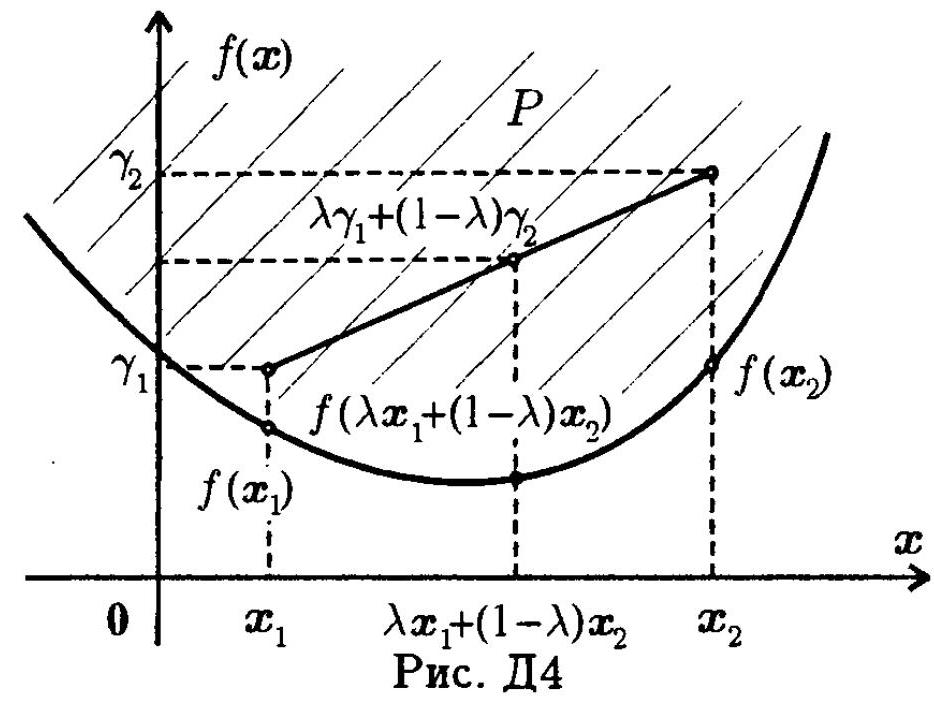
\includegraphics[max width=0.9\textwidth]{images/bo_d547okref24c73bgfch0_197_258_0_934_705_0.jpg}
\end{center}
\hspace*{3em} 

Теорема 1. Ecnu функция f : Е" → Е" выпукла и конеч- на, то она субдифференцируема в любой точке хе Е", т.е. \(\partial f\left( \mathbf{x}\right)  \neq  \varnothing\) ,и ее субдифференциал д \(f\left( \mathbf{x}\right)\) является множеством компактным и выпуклым.

Доказательство. Покажем сначала, что множество \(\partial f\left( {\mathbf{x}}_{0}\right)\) непусто.

Рассмотрим в пространстве E1 Х E’ множество точек, лежа- щих выше графика функции f(x) (рис. Д4). Такое множество называется надграфиком функции \(f\left( \mathbf{x}\right)\) и определяется как мно- жество

\[
P = \left\{  {\left( {\gamma ,\mathbf{x}}\right)  \in  {E}^{1} \times  {E}^{n} : \gamma  \geq  f\left( \mathbf{x}\right) }\right\}  .
\]

Ясно, что множество Р замкнуто. Действительно, пусть после- довательность точек ( \({\gamma }_{n},{\mathbf{x}}_{n}\) ) \(\in  P\) cxoдится к точке \(\left( {\gamma ,\mathbf{x}}\right)  \in\) ∈ \({E}^{1} \times  {E}^{n}\) . По определению надграфика выполняется неравен- ство γ…денего. Поскольку функция \(f\left( \mathbf{x}\right)\) непрерывна (см. те- opemy 1 из раздела Д3), получаем γ ≥ \(f\left( \mathbf{x}\right)\) , т.е. точка (γ, x) принадлежит множеству \(P\) .

Покажем, что множество \(P\) выпукло. Пусть заданы точки \(\left( {{\gamma }_{1},{\mathbf{x}}_{1}}\right) ,\left( {{\gamma }_{2},{\mathbf{x}}_{2}}\right)  \in  P\) и число 0 < λ< 1. Corлacно определению множества \(P\) имеем неравенства \({\gamma }_{1} \geq  f\left( {\mathbf{x}}_{1}\right) ,{\gamma }_{2} \geq  f\left( {\mathbf{x}}_{2}\right)\) . По- скольку функция \(f\left( \mathbf{x}\right)\) выпукла,

\[
\lambda {\gamma }_{1} + \left( {1 - \lambda }\right) {\gamma }_{2} \geq  {\lambda f}\left( {\mathbf{x}}_{1}\right)  + \left( {1 - \lambda }\right) f\left( {\mathbf{x}}_{2}\right)  \geq  f\left( {\lambda {\mathbf{x}}_{1} + \left( {1 - \lambda }\right) {\mathbf{x}}_{2}}\right) ,
\]

T.e.

\[
\lambda \left( {{\gamma }_{1},{\mathbf{x}}_{1}}\right)  + \left( {1 - \lambda }\right) \left( {{\gamma }_{2},{\mathbf{x}}_{2}}\right)  \in  P.
\]

Таким образом, множество Р есть выпуклое и замкнутое подмножество пространства E1 X En. Pacсмотрим произволь- ную точку \({\mathbf{x}}_{0} \in  {E}^{n}\) . Toчка \(\left( {f\left( {\mathbf{x}}_{0}\right) ,{\mathbf{x}}_{0}}\right)\) принадлежит множеству \(P\) ,но не принадлежит внутренности множества \(P\) ,поскольку последовательность точек (f( \({\mathbf{x}}_{0}\) ) – k \({\mathbf{x}}_{0}\) ) не принадлежит мно- жеству \(P\) ни при каком \(k\) и сходится к точке \(\left( {f\left( {\mathbf{x}}_{0}\right) ,{\mathbf{x}}_{0}}\right)\) при \(k \rightarrow  \infty\) . Согласно лемме об отделимости (см. раздел Д2) мно- жество \(P\) и точка \(\left( {f\left( {\mathbf{x}}_{0}\right) ,{\mathbf{x}}_{0}}\right)\) отделимы в пространстве E \({}^{1} \times  {E}^{n}\) , т.е. существует единичный вектор \(\left( {\lambda ,\psi }\right)  \in  {E}^{1} \times  {E}^{n}\) такой,что для всех точек \(\left( {\lambda ,\mathbf{x}}\right)  \in  P\) выполняется неравенство

\[
{\gamma \lambda } + \langle \mathbf{x},\psi \rangle  \leq  f\left( {\mathbf{x}}_{0}\right) \lambda  + \left\langle  {{\mathbf{x}}_{0},\psi }\right\rangle  .
\]
 (Д.26)

\begin{center}
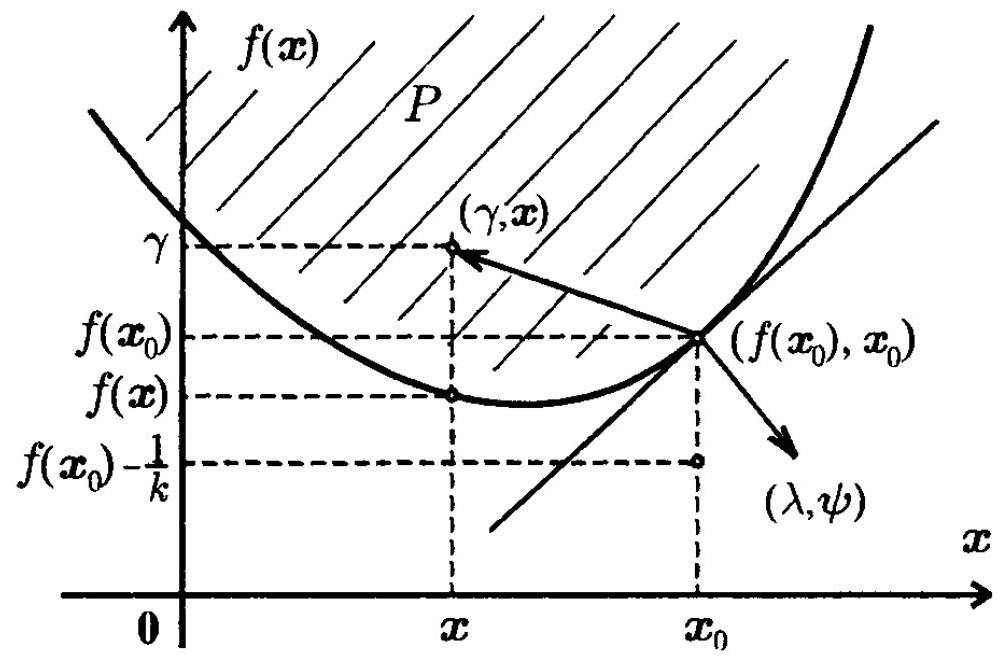
\includegraphics[max width=0.9\textwidth]{images/bo_d547okref24c73bgfch0_198_231_0_1003_657_0.jpg}
\end{center}
\hspace*{3em} 

Рис. Д5

(рис. ДБ). При \(x = {x}_{0}\) и \(\gamma  \geq  f\left( {x}_{0}\right)\) из этого неравенства полу- чаем \({\gamma \lambda } \leq  f\left( {x}_{0}\right) \lambda\) ,т.е. \(\lambda  \leq  0\) . Ecn же λ = 0, to неравенство (Д.26) принимает вид \(\langle \mathbf{x},\mathbf{\psi }\rangle  \leq  \left\langle  {{\mathbf{x}}_{0},\mathbf{\psi }}\right\rangle\) . Последнее неравенст- во может выполняться для всех х ∈ \({E}^{n}\) только тогда, когда \(\psi  = 0\) . A это невозможно, trak как вектор \(\left( {\lambda ,\psi }\right)  \in  {E}^{n + 1}\) имеет единичную длину. Следовательно, в неравенстве (Д.26) число \(\lambda\) отрицательно. Разделив это неравенство на \(\lambda\) и подставив в него точку (f(x)). х) е р, получим неравенство

\[
\left\langle  {-\frac{\psi }{\lambda },\mathbf{x} - {\mathbf{x}}_{0}}\right\rangle   \leq  f\left( \mathbf{x}\right)  - f\left( {\mathbf{x}}_{0}\right) ,
\]

которое выполняется при всех х ∈ E". Следовательно, вектор \(- \frac{\psi }{\lambda } \in  {E}^{n}\) принадлежит субдифференциалу д \(f\left( {\mathbf{x}}_{0}\right)\) функции \(f\left( \mathbf{x}\right)\) в точке хо (см. формулу (Д.25)), т.е. д \(f\left( \mathbf{x}\right)  \neq  \varnothing\) и функция \(f\left( \mathbf{x}\right)\) субдифференцируема в любой точке \({\mathbf{x}}_{0} \in  {E}^{n}\) .

Покажем теперь, что множество д \(f\left( {\mathbf{x}}_{0}\right)\) замкнуто. Пусть по- следовательность точек \({\mathbf{p}}_{k} \in  \partial f\left( {\mathbf{x}}_{0}\right)\) cxoдится к точке \(\mathbf{p} \in  {E}^{n}\) . В силу формулы (Д.25) имеем неравенство

\[
\left\langle  {{\mathbf{p}}_{k},\mathbf{x} - {\mathbf{x}}_{0}}\right\rangle   \leq  f\left( \mathbf{x}\right)  - f\left( {\mathbf{x}}_{0}\right) ,
\]

справедливое при всех х € Е". Переходя в этом неравенстве к пределу, получим \(\left\langle  {\mathbf{p},\mathbf{x} - {\mathbf{x}}_{0}}\right\rangle   \leq  f\left( \mathbf{x}\right)  - f\left( {\mathbf{x}}_{0}\right)\) , т.е. р е д \(f\left( {\mathbf{x}}_{0}\right)\) . Докажем ограниченность множества д \(f\left( {\mathbf{x}}_{0}\right)\) . Предположим про- тивное, т.е. существует последовательность точек \({\mathbf{p}}_{k} \in  \partial f\left( {\mathbf{x}}_{0}\right)\) такая, что \(\left\lVert \begin{array}{c} {\mathbf{p}}_{k} \end{array} \right\rVert \rightarrow   + \infty\) при \(k \rightarrow   + \infty\) . B силу формулы (A.25) при всех х ∈ \({E}^{n}\) выполняется неравенство

\[
\left\langle  {{\mathbf{p}}_{k},\mathbf{x} - {\mathbf{x}}_{0}}\right\rangle   \leq  f\left( \mathbf{x}\right)  - f\left( {\mathbf{x}}_{0}\right) .
\]

Подставив в это неравенство для каждого к точку хе хоч — получим \(\left\lVert \begin{array}{c} {\mathbf{p}}_{k} \end{array} \right\rVert \leq  f\left( {\mathbf{x}}_{k}\right)  - f\left( {\mathbf{x}}_{0}\right)\) . Toчки x, принадлежат компакт- ному шару \({S}_{1}\left( \mathbf{0}\right)\) . Функция \(f\left( \mathbf{x}\right)\) непрерывна согласно теореме 1 (см. раздел ДЗ). Поэтому правая часть последнего неравенства ограничена на множестве \({S}_{1}\left( {\mathbf{x}}_{0}\right)\) . A это противоречит предпо- ложению о том,что \(\left\lVert \begin{array}{c} {\mathbf{p}}_{k} \end{array} \right\rVert \rightarrow   + \infty\) при \(k \rightarrow  \infty\) .

Осталось доказать выпуклость множества ∂f(x). Пусть \({\mathbf{p}}_{1},{\mathbf{p}}_{2} \in  \partial f\left( {\mathbf{x}}_{0}\right)\) и \(0 \leq  \lambda  \leq  1\) . Тогда в силу формулы (II.25) при всех х ∈ \({E}^{n}\) выполняются неравенства

\[
\left\langle  {{\mathbf{p}}_{1},\mathbf{x} - {\mathbf{x}}_{0}}\right\rangle   \leq  f\left( \mathbf{x}\right)  - f\left( {\mathbf{x}}_{0}\right) ,\;\left\langle  {{\mathbf{p}}_{2},\mathbf{x} - {\mathbf{x}}_{0}}\right\rangle   \leq  f\left( \mathbf{x}\right)  - f\left( {\mathbf{x}}_{0}\right) .
\]

Умножая эти неравенства на \(\lambda\) и \(1 - \lambda\) coответственно и скла- дывая, получаем при всех х ∈ \({E}^{n}\) соотношение

\[
\left\langle  {\lambda {\mathbf{p}}_{1} + \left( {1 - \lambda }\right) {\mathbf{p}}_{2},\mathbf{x} - {\mathbf{x}}_{0}}\right\rangle   \leq  f\left( \mathbf{x}\right)  - f\left( {\mathbf{x}}_{0}\right) .
\]

Cледовательно, \(\lambda {\mathbf{p}}_{1} + \left( {1 - \lambda }\right) {\mathbf{p}}_{2} \in  \partial f\left( {\mathbf{x}}_{0}\right)\) и теорема полностью доказана.

Следствие. Для любого множества F € Ω(E’n) опорная функция \(c\left( {F,\psi }\right) {cy6}\partial u\oint {\phi epe}\) нцируема в любой точке \({\psi }_{0} \in  {E}^{n}\) и ее субдифференциал дс \(\left( {F,{\psi }_{0}}\right)\) является множеством выпук- лым и компактным.

Теорема 2. Пусть функция \(f : {E}^{n} \rightarrow  {E}^{1}\) конечна. В этом случае функция \(f\left( \mathbf{\psi }\right)\) является опорной к некоторому выпук- лому множеству \(F \in  \Omega \left( {E}^{n}\right)\) morda и только тогда, когда выполняются следующие два условия:

1) \(f\left( {\lambda \psi }\right)  = {\lambda f}\left( \psi \right) ,\lambda  \geq  0\) ;

2) \(f\left( {{\psi }_{1} + {\psi }_{2}}\right)  \leq  f\left( {\psi }_{1}\right)  + f\left( {\psi }_{2}\right)\) .

При эпом миожесгиеегимееп ечd

\[
F = \left\{  {\mathbf{f} \in  {E}^{n} : \langle \mathbf{f},\mathbf{\psi }\rangle  \leq  f\left( \mathbf{\psi }\right) \forall \mathbf{\psi } \in  {E}^{n}}\right\}  .
\]
 (Д.27)

Доказательство. Если функция \(f\left( \psi \right)\) является опорной к некоторому множеству \(F \in  \Omega \left( {E}^{n}\right)\) , то она конечна и удовле- творяет условиям 1 и 2 (см. свойства 1 и 2 опорных функций, лекция 3).

Докажем утверждение теоремы в другую сторону. Функция \(f\left( \psi \right)\) конечна и выпукла, так как из условий 1 и 2 при всех \({\psi }_{1},{\psi }_{2} \in  {E}^{n}\) следует неравенство

\[
f\left( {\lambda {\psi }_{1} + \left( {1 - \lambda }\right) {\psi }_{2}}\right)  \leq  f\left( {\lambda {\psi }_{1}}\right)  + f\left( {\left( {1 - \lambda }\right) {\psi }_{2}}\right)  = {\lambda f}\left( {\psi }_{1}\right)  + \left( {1 - \lambda }\right) f\left( {\psi }_{2}\right) .
\]

Поэтому согласно теореме 1 она субдифференцируема в любой точке \({\mathbf{\psi }}_{0} \in  {E}^{n}\) . Множество F, заданное формулой (Д.27), есть не что иное, как субдифференциал функции \(f\left( \mathbf{\psi }\right)\) в точке \({\mathbf{\psi }}_{0} = \mathbf{0}\) (сравните с формулой (Д.25)). Следовательно, в силу теоремы 1 это множество \(F\) выпукло и компактно.

Рассмотрим опорную функцию \(c\left( {F,\psi }\right)\) этого множества F. Если показать, что \(c\left( {F,\mathbf{\psi }}\right)  \equiv  f\left( \mathbf{\psi }\right)\) , то теорема будет доказана.

Используя формулу (Д.27), получим для любого вектора \(\psi  \in  {E}^{n}\) неравенство

\[
c\left( {F,\psi }\right)  = \mathop{\max }\limits_{{f \in  F}}\langle f,\psi \rangle  \leq  f\left( \psi \right) .
\]

Для доказательства равенства в этом соотношении предполо- жим противное, т.е. пусть существует вектор \(\overline{\mathbf{\psi }} \in  {E}^{n}\) такой,что \(c\left( {F,\overline{\mathbf{\psi }}}\right)  < \langle \mathbf{f},\overline{\mathbf{\psi }}\rangle\) . Cor.racно теореме 1 множество д \(f\left( \overline{\mathbf{\psi }}\right)\) непусто. Для вектора \(p \in  \partial f\left( \overline{\psi }\right)\) имеем неравенство

\[
\langle \mathbf{p},\psi  - \overline{\psi }\rangle  \leq  f\left( \psi \right)  - f\left( \overline{\psi }\right) ,
\]
 (Д.28)

справедливое при всех у не в год Из условия 2 следует, что

\[
f\left( \psi \right)  = f\left( {\psi  - \overline{\psi } + \overline{\psi }}\right)  \leq  f\left( {\psi  - \overline{\psi }}\right)  + f\left( \overline{\psi }\right) ,
\]

т.е. \(f\left( \psi \right)  - f\left( \overline{\psi }\right)  \leq  f\left( {\psi  - \overline{\psi }}\right)\) . Поэтому из неравенства (II.28) получаем неравенство \(\langle \mathbf{p},\mathbf{\psi } - \overline{\mathbf{\psi }}\rangle  \leq  f\left( {\mathbf{\psi } - \overline{\mathbf{\psi }}}\right)\) , cnpaведливое для любого вектора ψ ∈ \({E}^{n}\) , следовательно, для любого вектора \(\mathbf{\psi } - \overline{\mathbf{\psi }} \in  {E}^{n}\) . Это означает, что ре дб(0) = F.

Corлacно условию 1 имеем \(f\left( 0\right)  = 0\) . Поэтому,положив в неравенстве (П.28) \(\psi  = 0\) , noлучим \(\langle \mathbf{p},\overline{\psi }\rangle  \geq  f\left( \overline{\psi }\right)  > c\left( {F,\overline{\psi }}\right)\) . Это означает согласно следствию из свойства 6 опорных функций (см. лекцию 3), что р е н Г. Полученное противоречие доказыва- ет теорему.

Теорема 3. Пусть функция f : Е" → Е" выпукла и ко- нечна. Тогда для любой точки х ∈ Е" опорная функция суб- \(\partial u\partial \phi\) беренциала д \(f\left( \mathbf{x}\right)\) в направлениии вектора ψ ∈ \({E}^{n}\) имеет вид

\[
c\left( {\partial f\left( \mathbf{x}\right) ,\psi }\right)  = {f}^{\prime }\left( {\mathbf{x};\psi }\right) .
\]

Доказательство. По теореме 2 (см. раздел Д2) производ- ная \({f}^{\prime }\left( {\mathbf{x};\mathbf{\psi }}\right)\) or функции \(f\left( \mathbf{x}\right)\) в точке \(\mathbf{x} \in  {E}^{n}\) по любому направ- лению \(\psi  \in  {E}^{n}\) cyществует и удовлетворяет двум свойствам:

1) \({f}^{\prime }\left( {\mathbf{x};\lambda \mathbf{\psi }}\right)  = \lambda {f}^{\prime }\left( {\mathbf{x};\mathbf{\psi }}\right) ,\lambda  \geq  0\) ;

2) \({f}^{\prime }\left( {\mathbf{x};{\mathbf{\psi }}_{1} + {\mathbf{\psi }}_{2}}\right)  \leq  {f}^{\prime }\left( {\mathbf{x};{\mathbf{\psi }}_{1}}\right)  + {f}^{\prime }\left( {\mathbf{x};{\mathbf{\psi }}_{2}}\right)\) .

Следовательно, согласно теореме 2 функция \({f}^{\prime }\left( {\mathbf{x};\mathbf{\psi }}\right)\) являет- ся опорной к множеству

\[
F = \left\{  {\mathbf{f} \in  {E}^{n} : \langle \mathbf{f},\mathbf{\psi }\rangle  \leq  {f}^{\prime }\left( {\mathbf{x};\mathbf{\psi }}\right) \;\forall \mathbf{\psi } \in  {E}^{n}}\right\}  .
\]

Остается доказать, что множества дб(х) и F совпадают. Со- гласно определению производной по направлению имеем соот- ношение

\[
F = \left\{  {\mathbf{f} \in  {E}^{n} : \langle \mathbf{f},\mathbf{\psi }\rangle  \leq  \mathop{\lim }\limits_{{\alpha  \rightarrow   + 0}}\frac{f\left( {\mathbf{x} + \alpha \mathbf{\psi }}\right)  - f\left( \mathbf{x}\right) }{\alpha }\;\forall \mathbf{\psi } \in  {E}^{n}}\right\}  .
\]

Согласно теореме 2 (см. раздел ДЗ) для выпуклой функции \(f\left( \mathbf{x}\right)\) величина \(\varphi \left( \alpha \right)  = \frac{f\left( {x + {\alpha \psi }}\right)  - f\left( x\right) }{\alpha }\) не возрастает при \(\alpha  \rightarrow   + 0\) . Поэ- тому имеем равенство

\[
F = \left\{  {\mathbf{f} \in  {E}^{n} : \langle \mathbf{f},\mathbf{\psi }\rangle  \leq  \frac{f\left( {\mathbf{x} + \alpha \mathbf{\psi }}\right)  - f\left( \mathbf{x}\right) }{\alpha }\;\forall \alpha  > 0,\forall \mathbf{\psi } \in  {E}^{n}}\right\}   =
\]

\[
= \left\{  {\mathbf{f} \in  {E}^{n} : \langle \mathbf{f},\alpha \mathbf{\psi }\rangle  \leq  f\left( {\mathbf{x} + \alpha \mathbf{\psi }}\right)  - f\left( \mathbf{x}\right) \;\forall \alpha  > 0,\forall \mathbf{\psi } \in  {E}^{n}}\right\}  .
\]

Положив \(\mathbf{y} = \mathbf{x} + \alpha \mathbf{\psi }\) ,получим соотношение

\[
F = \left\{  {\mathbf{f} \in  {E}^{n} : \langle \mathbf{f},\mathbf{y} - \mathbf{x}\rangle  \leq  f\left( \mathbf{y}\right)  - f\left( \mathbf{x}\right) \;\forall \mathbf{y} \in  {E}^{n}}\right\}   = \partial f\left( \mathbf{x}\right) ,
\]

и теорема доказана.

Следствие. Для любого множества F € Ω(E’) опорная функция субдифференциала дс \(\left( {F,{\psi }_{0}}\right)\) в точке ну ве точке ф \({\psi }_{0} \in  {E}^{n}\) в на- правлении вектора ψ с Ев имеет вид

\[
c\left( {\partial c\left( {F,{\psi }_{0}}\right) ,\psi }\right)  = {c}^{\prime }\left( {F,{\psi }_{0};\psi }\right) .
\]

Теорема 4. Пусть функция f : Е" → Е" выпукла и конечна. В этом случае функция f(x) дифференцируема в точке \({\mathbf{x}}_{0} \in  {E}^{n}\) тогда и только тогда, когда ее субдиффе- ренциал в этой точке состоит из единственного вектора \(\partial f\left( {\mathbf{x}}_{0}\right)  = \left\{  \frac{\partial f\left( {\mathbf{x}}_{0}\right) }{\partial \mathbf{x}}\right\}  .\)

Доказательство. Пусть функция \(f\left( \mathbf{x}\right)\) дифференцируема в точке \({x}_{0}\) и \(\frac{\partial f\left( {x}_{0}\right) }{\partial x}\) - ee градиент. Тогда производная по на- правлению \({f}^{\prime }\left( {{\mathbf{x}}_{0};\mathbf{\psi }}\right)\) имеет вид

\[
{f}^{\prime }\left( {{\mathbf{x}}_{0};\psi }\right)  = \left\langle  {\frac{\partial f\left( {\mathbf{x}}_{0}\right) }{\partial \mathbf{x}},\psi }\right\rangle  .
\]

Согласно теореме 3 получим

\[
c\left( {\partial f\left( {\mathbf{x}}_{0}\right) ,\psi }\right)  = \left\langle  {\frac{\partial f\left( {\mathbf{x}}_{0}\right) }{\partial \mathbf{x}},\psi }\right\rangle  ,
\]

т.е. опорные функции выпуклых множеств дб( \({\mathbf{x}}_{0}\) ) и \{ \(\frac{\partial f\left( {\mathbf{x}}_{0}\right) }{\partial \mathbf{x}}\) \} cos- падают. Следовательно, в силу следствия из свойства 11 опор- ных функций (см. лекцию 3) множества дб(к0) и \{ \(\frac{\partial f\left( {x}_{0}\right) }{\partial x}\) \} cos- падают, т.е. субдифференциал д \(f\left( {\mathbf{x}}_{0}\right)\) cocтоит из единственного вектора дбк)

Пусть теперь субдифференциал \(\partial f\left( {\mathbf{x}}_{0}\right)\) состоит из единст- венного вектора \(p \in  {E}^{n}\) . В этом случае из теоремы 3 следу- ет, что для любого вектора ф € Е" выполняется равенство \({f}^{\prime }\left( {{\mathbf{x}}_{0};\mathbf{\psi }}\right)  = \langle \mathbf{p},\mathbf{\psi }\rangle\) . Учитывая определение производной по на- правлению, видно, что для любого числа а > 0 и любого вектора \(\psi  \in  {E}^{n}\) выполняется соотношение

\[
f\left( {{\mathbf{x}}_{0} + \alpha \mathbf{\psi }}\right)  - f\left( {\mathbf{x}}_{0}\right)  = \alpha \langle \mathbf{p},\mathbf{\psi }\rangle  + \bar{o}\left( \alpha \right) .
\]
 (Д.29)

Покажем, что функция \(f\left( \mathbf{x}\right)\) дифференцируема в точке хо и вектор \(\mathbf{p}\) есть ее градиент. Для этого нужно доказать, что выполняется соотношение

\[
f\left( \mathbf{x}\right)  - f\left( {\mathbf{x}}_{0}\right)  - \left\langle  {\mathbf{p},\mathbf{x} - {\mathbf{x}}_{0}}\right\rangle   = \bar{o}\left( \left\lVert \begin{array}{c} {\mathbf{x} - {\mathbf{x}}_{0}} \end{array} \right\rVert\right) .
\]

Поскольку \(f\left( \mathbf{x}\right)  - f\left( {\mathbf{x}}_{0}\right)  - \left\langle  {\mathbf{p},\mathbf{x} - {\mathbf{x}}_{0}}\right\rangle   \geq  0\) corracно определе- нию субдифференциала р (см. формулу (Д.25)), достаточно по- казать, что

\[
f\left( \mathbf{x}\right)  - f\left( {\mathbf{x}}_{0}\right)  - \left\langle  {\mathbf{p},\mathbf{x} - {\mathbf{x}}_{0}}\right\rangle   \leq  \bar{o}\left( \left\lVert \begin{array}{c} {\mathbf{x} - {\mathbf{x}}_{0}} \end{array} \right\rVert\right) .
\]
 (Д.30)

При доказательстве теоремы 1 (см. раздел ДЗ) для вектора приращения \({\Delta x} = x - {x}_{0}\) было построено разложение

\[
\mathbf{x} - {\mathbf{x}}_{0} = {\xi }_{1}{e}_{1} + \ldots  + {\xi }_{2n}{e}_{2n}
\]

(см. формулу (Д.18) из раздела Д3) по векторам е, г…о, его его, причем числа \({\xi }_{i}\) удовлетворяли условию 0 ≤ \({\xi }_{i} \leq  \left\lVert \begin{array}{c} {\mathbf{x} - {\mathbf{x}}_{0}} \end{array} \right\rVert\) , a следовательно, и условию ō \(\left( {\xi }_{i}\right)  \leq  \bar{o}\left( \left\lVert \begin{array}{c} {\mathbf{x} - {\mathbf{x}}_{0}} \end{array} \right\rVert\right)\) . Более того, для приращения функции \(f\left( {\mathbf{x} + \mathbf{{\Delta x}}}\right)\) была получена оценка

\[
f\left( {\mathbf{x} + \mathbf{\Delta }\mathbf{x}}\right)  \leq  \frac{1}{2n}\mathop{\sum }\limits_{{i = 1}}^{{2n}}f\left( {{\mathbf{x}}_{0} + {\xi }_{i}{2n}{\mathbf{e}}_{i}}\right) .
\]

Следовательно,

\[
f\left( \mathbf{x}\right)  - f\left( {\mathbf{x}}_{0}\right)  \leq  \frac{1}{2n}\mathop{\sum }\limits_{{i = 1}}^{{2n}}\left\lbrack  {f\left( {{\mathbf{x}}_{0} + {\xi }_{i}{2n}{\mathbf{e}}_{i}}\right)  - f\left( {\mathbf{x}}_{0}\right) }\right\rbrack  .
\]
 (Д.31)

Каждое слагаемое под знаком суммы в этом неравенстве либо равно нулю, если бы он, не знаю если бы у онос не знают не ставлено согласно формуле (Д.29) в виде

\[
f\left( {{\mathbf{x}}_{0} + {\xi }_{i}{2n}{e}_{i}}\right)  - f\left( {\mathbf{x}}_{0}\right)  = {\xi }_{i}\left\langle  {\mathbf{p},{2n}{e}_{i}}\right\rangle   + \bar{o}\left( {\xi }_{i}\right) .
\]

Следовательно, с учетом соотношения (Д.31) получим неравен- CTBO

\[
f\left( \mathbf{x}\right)  - f\left( {\mathbf{x}}_{0}\right)  \leq  \frac{1}{2n}\mathop{\sum }\limits_{{i = 1}}^{{2n}}\left\lbrack  {{\xi }_{i}\left\langle  {\mathbf{p},{2n}{\mathbf{e}}_{i}}\right\rangle   + \bar{o}\left( {\xi }_{i}\right) }\right\rbrack   \leq  \left\langle  {\mathbf{p},\mathbf{x} - {\mathbf{x}}_{0}}\right\rangle   + \bar{o}\left( \left\lVert \begin{array}{c} {\mathbf{x} - {\mathbf{x}}_{0}} \end{array} \right\rVert\right) ,
\]

т.е. оценка (Д.30) доказана. Этим завершается доказательство теоремы.

Мы исследовали некоторые основные свойства субдифферен- циала д \(f\left( {\mathbf{x}}_{0}\right)\) от выпуклой функции \(f\left( \mathbf{x}\right)\) . Кроме перечисленных, субдифференциал обладает еще целым рядом замечательных свойств. Можно даже построить целое субдифференциальное исчисление. Но все это не является предметом наших исследова- ний. Заметим только, что в настоящее время субдифференциа- лы выпуклых функций находят широкое применение во многих областях математики.

Задачи

1. Пусть \({f}_{1}\left( x\right) ,{f}_{2}\left( x\right)\) - выпуклые и конечные функции и \({\lambda }_{1},{\lambda }_{2} \geq  0\) . Докажите равенство

\[
\partial \left( {{\lambda }_{1}{f}_{1}\left( \mathbf{x}\right)  + {\lambda }_{2}{f}_{2}\left( \mathbf{x}\right) }\right)  = {\lambda }_{1}\partial {f}_{1}\left( \mathbf{x}\right)  + {\lambda }_{2}\partial {f}_{2}\left( \mathbf{x}\right) .
\]

2. Пусть \(A : {E}^{n} \rightarrow  {E}^{m}\) - ограниченный линейный оператор, заданный матрицей \(A\) , a функция \(f : {E}^{m} \rightarrow  {E}^{1}\) выпукла и конечна. Докажите, что

\[
\partial \left( {{Af}\left( \mathbf{x}\right) }\right)  = {A}^{ * }\partial f\left( \mathbf{x}\right) .
\]

3. Докажите, что выпуклая и конечная функция \(f : {E}^{n} \rightarrow  {E}^{1}\) достигает минимума в точке \({\mathbf{x}}_{0} \in  {E}^{n}\) тогда и только тогда, когда 0 ∈ \(\partial f\left( {\mathbf{x}}_{0}\right)\) . Сравните с аналогичным фактом для гладкой функции, когда 0 = \(\frac{\partial f\left( {x}_{0}\right) }{\partial x}\) .

4*. Пусть функция \(f : {E}^{n} \rightarrow  {E}^{1}\) выпукла и конечна. Дока- жите, что ее субдифференциал \(\partial f\left( \mathbf{x}\right)\) является полунепрерыв- ным сверху многозначным отображением, т.е. для любой точки \({\mathbf{x}}_{0} \in  {E}^{n}\) и любого числа ε > 0 существует число δ > 0 такое, что при всех х таких, что || \(x - {x}_{0}\parallel  \leq  \delta\) ,выполняется включение

\[
\partial f\left( \mathbf{x}\right)  \subset  \partial f\left( {\mathbf{x}}_{0}\right)  + {S}_{\varepsilon }\left( \mathbf{0}\right) .
\]

\section*{Д5. Опорное множество}

Опорным множеством (см. лекцию 3, рис. 7 и рис. Д5) для множества \(F \in  \Omega \left( {E}^{n}\right)\) в направлении \(\psi  \in  {E}^{n}\) называется мно- жество всех векторов \({\mathbf{f}}_{0} \in  F\) ,на которых достигается максимум в опорной функции

\[
c\left( {F,{\psi }_{0}}\right)  = \mathop{\max }\limits_{{f \in  F}}\left\langle  {f,{\psi }_{0}}\right\rangle  .
\]

Обозначивэто опорное множество через \(\mathcal{U}\left( {F,{\psi }_{0}}\right)\) ,имеем

\[
\mathcal{U}\left( {F,{\psi }_{0}}\right)  = \left\{  {\mathbf{f} \in  F : \left\langle  {\mathbf{f},{\mathbf{\psi }}_{0}}\right\rangle   = c\left( {F,{\mathbf{\psi }}_{0}}\right) }\right\}  . \tag{A.32}
\]

Очевидно,что если но,, te 0, то опорное множество \(\mathcal{U}\left( {F,{\psi }_{0}}\right)\) ecть пересечение множества F и опорной гиперплоскости

\[
{\Gamma }_{{\psi }_{0}} = \left\{  {\mathbf{f} \in  {E}^{n} : \left\langle  {\mathbf{f},{\mathbf{\psi }}_{0}}\right\rangle   = c\left( {F,{\psi }_{0}}\right) }\right\}  .
\]
 (Д.33)

\begin{center}
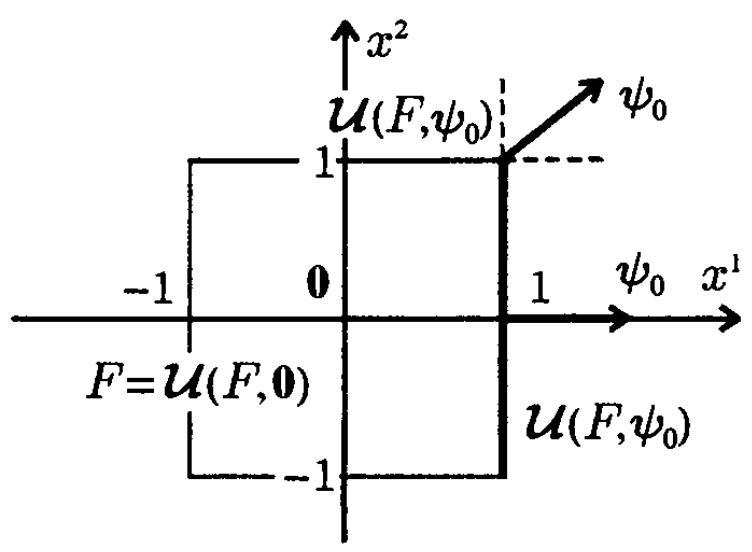
\includegraphics[max width=0.7\textwidth]{images/bo_d547okref24c73bgfch0_205_0_0_752_552_0.jpg}
\end{center}
\hspace*{3em} 

Рис. Д6

Ecm же \({\psi }_{0} = 0,\) To \(\mathcal{U}\left( {F,{\psi }_{0}}\right)  = F\) . Поэтому \(\mathcal{U}\left( {F,{\psi }_{0}}\right)  \in  \Omega \left( {E}^{n}\right)\) ,т.е. мно- жество \(\mathcal{U}\left( {F,{\psi }_{0}}\right)\) является не- пустым и компактным. Более того, если множество \(F\) вы- пукло, то и его опорное мно- жество \(\mathcal{U}\left( {F,{\psi }_{0}}\right)\) также вы- пукло.

Пример 1. Пусть мно- жество \(F \in  \Omega \left( {E}^{n}\right)\) задано ycnobuem

\[
F = \left\{  {\mathbf{x} \in  {E}^{2} : \left| {x}^{1}\right|  \leq  1,\left| {x}^{2}\right|  \leq  1}\right\}  .
\]

Это есть квадрат на плоскости со сторонами, параллель- ными осям координат (рис. Дб). Ясно, что если ни одна из координат \({\psi }^{1},{\psi }^{2}\) вектора \(\psi\) не равна нулю, то опорное множес- тво И(К, 杓) состоит из единственной точки (sign \({\psi }^{1}\) , sign \({\psi }^{2}\) ). B остальных случаях опорное множество задается соотношениями

\[
\mathcal{U}\left( {F,\psi }\right)  = \left\{  \begin{array}{ll} \left\{  {\mathbf{x} \in  {E}^{2} : {x}^{1} = \operatorname{sign}{\psi }^{1},\left| {x}^{2}\right|  \leq  1}\right\}  , & {\psi }^{1} \neq  0,{\psi }^{2} = 0, \\  \left\{  {\mathbf{x} \in  {E}^{2} : \left| {x}^{1}\right|  \leq  1,{\mathbf{x}}^{2} = \operatorname{sign}{\psi }^{2}}\right\}  , & {\psi }^{1} = 0,{\psi }^{2} \neq  0, \\  F, & {\psi }^{1} = 0,{\psi }^{2} = 0. \end{array}\right.
\]

\iffalse

Теорема 1. Пусмь забано множесгееспео F \(\in  \Omega \left( {E}^{n}\right) u\) ezo onop-raz [tynkyuk c(F,ψ). Tozda ebinyknas obonouka conv \(\mathcal{U}\left( {F,{\psi }_{0}}\right)\) onophozo whoskecmea \(\mathcal{U}\left( {F,{\psi }_{0}}\right)  \in\) nanpasnenuu \({\psi }_{0} \in  {E}^{n}\) coena- \(\left\lbrack  \begin{array}{cccccc} \partial a & e & m & c & c & y \\  6 & \partial u & \phi & \phi & e & p \\  e & u & u & u & a & n \\  \omega & a & \left( {F,{\psi }_{0}}\right) & {on} & o & p \\  u & o & u & \phi & y & u \\  x & y & u & u & v & u \end{array}\right\rbrack  \left\lbrack  \begin{array}{c} c\left( {F,\psi }\right) \end{array}\right\rbrack\) e mouxe \({\psi }_{0}\) , т.е.

\[
\operatorname{conv}\mathcal{U}\left( {F,{\psi }_{0}}\right)  = \partial c\left( {F,{\psi }_{0}}\right) .
\]
 (Д.34)

Доказательство. Вспомним, что субдифференциал опор- ной функции задается соотношением

\[
\partial c\left( {F,{\psi }_{0}}\right)  = \left\{  {f \in  {E}^{n} : \left\langle  {f,\psi  - {\psi }_{0}}\right\rangle   \leq  }\right.
\]

\[
\leq  c\left( {F,\psi }\right)  - c\left( {F,{\psi }_{0}}\right) \;\forall \psi  \in  {E}^{n}\} .
\]
 (Д.35)

Покажем сначала, что выполняется включение

\[
\mathcal{U}\left( {F,{\psi }_{0}}\right)  \subset  \partial c\left( {F,{\psi }_{0}}\right) .
\]
 (Д.36)

Пусть \(f \in  \mathcal{U}\left( {F,{\psi }_{0}}\right)\) , тогда из формулы (II.32) следует, что \(f \in  F,\left\langle  {f,{\psi }_{0}}\right\rangle   = c\left( {F,{\psi }_{0}}\right)\) . В силу следствия из свойства 6 опорных функций (см. лекцию 3) для любого вектора ф ∈ Ег выполняется неравенство \(\langle \mathbf{f},\mathbf{\psi }\rangle  \leq  c\left( {F,\mathbf{\psi }}\right)\) . Oтсюда получаем соотношение

\[
\langle \mathbf{f},\mathbf{\psi }\rangle  - \left\langle  {\mathbf{f},{\mathbf{\psi }}_{0}}\right\rangle   \leq  c\left( {F,\mathbf{\psi }}\right)  - c\left( {F,{\mathbf{\psi }}_{0}}\right) .
\]

Это значит, что вектор f принадлежит субдифференциалу \(\partial c\left( {F,{\mathbf{\psi }}_{0}}\right)\) (см. формулу (II.35)),и включение (II.36) доказано.

Докажем теперь включение

\[
\partial c\left( {F,{\psi }_{0}}\right)  \subset  \operatorname{conv}F
\]
 (Д.37)

Пусть \(f \in  \partial c\left( {F,{\psi }_{0}}\right)\) . Используя формулу (Д.35) и свойство 2 опорных функций (см. лекцию 3), для любого вектора ф ∈ Ег получаем неравенство

\[
\left\langle  {\mathbf{f},\mathbf{\psi } - {\mathbf{\psi }}_{0}}\right\rangle   \leq  c\left( {F,\mathbf{\psi }}\right)  - c\left( {F,{\mathbf{\psi }}_{0}}\right)  =
\]

\[
= c\left( {F,\psi  - {\psi }_{0} + {\psi }_{0}}\right)  - c\left( {F,{\psi }_{0}}\right)  \leq  c\left( {F,\psi  - {\psi }_{0}}\right) .
\]

Это значит, что для любого вектора h = ψ – ψ = Ег справед- ливо неравенство \(\langle \mathbf{f},\mathbf{h}\rangle  \leq  c\left( {F,\mathbf{h}}\right)\) . Oтсюда согласно свойству 9 опорных функций (см. лекцию 3) следует, что f ∈ conv F. Таким образом, включение (Д.37) доказано.

Докажем теперь включение

\[
\partial c\left( {F,{\psi }_{0}}\right)  \subset  {\Gamma }_{{\psi }_{0}}.
\]
 (Д.38)

Пусть \(f \in  \partial c\left( {F,{\psi }_{0}}\right)\) . Тогда для любого вектора ψ ∈ \({E}^{n}\) выполняется неравенство (см. формулу (Д.35))

\[
\left\langle  {f,\psi  - {\psi }_{0}}\right\rangle   \leq  c\left( {F,\psi }\right)  - c\left( {F,{\psi }_{0}}\right) .
\]

Положив в этом неравенстве ψ = 0 и ψ = 2 \({\psi }_{0}\) , получим соот- ветственно два неравенства — \(\left\langle  {\mathbf{f},{\psi }_{0}}\right\rangle   \leq   - c\left( {F,{\psi }_{0}}\right)\) и \(\left\langle  {\mathbf{f},{\psi }_{0}}\right\rangle   \leq \; \leq  c\left( {F,{\psi }_{0}}\right)\) ,т.е. получим равенство \(\left\langle  {\mathbf{f},{\psi }_{0}}\right\rangle   = c\left( {F,{\psi }_{0}}\right)\) . Cледова- тельно, в силу соотношения (Д.33) f ∈ \({\Gamma }_{{\psi }_{0}}\) и включение (Д.38) доказано.

Докажем теперь еще одно соотношение

\[
\operatorname{conv}F \cap  {\Gamma }_{{\psi }_{0}} = \operatorname{conv}\mathcal{U}\left( {F,{\psi }_{0}}\right) .
\]
 (Д.39)

Пусть \(f \in  \operatorname{conv}F \cap  {\Gamma }_{{\psi }_{0}}\) , Тогда \(f \in  \operatorname{conv}F\) и \(f \in  {\Gamma }_{{\psi }_{0}}\) . В разде- ле Д1 показано, что любая точка f из выпуклой оболочки conv F может быть представлена в виде

\[
f = {\lambda }_{1}{f}_{1} + \ldots  + {\lambda }_{n + 1}{f}_{n + 1},\;{f}_{i} \in  F,\;{\lambda }_{i} \geq  0,
\]

\[
{\lambda }_{1} + \ldots  + {\lambda }_{n + 1} = 1
\]
 (Д.40)

Поскольку \({f}_{i} \in  F\) , используя следствие из свойства 6 опорных функций (см. лекцию 3), можно написать n +1 неравенство

\[
\left\langle  {{\mathbf{f}}_{i},{\psi }_{0}}\right\rangle   \leq  c\left( {F,{\psi }_{0}}\right) ,\;i = 1,\ldots ,n + 1.
\]

В действительности во всех этих неравенствах выполняется равенство, так как если хотя бы в одном из них будет выпол- няться строгое неравенство, то, умножив эти неравенства на \({\lambda }_{i} \geq  0\) и сложив их, получим в силу формулы (A.40) строгое неравенство \(\left\langle  {\mathbf{f},{\mathbf{\psi }}_{0}}\right\rangle   < c\left( {F,{\mathbf{\psi }}_{0}}\right)\) ,что противоречит включению \(\mathbf{f} \in  {\Gamma }_{{\mathbf{\psi }}_{0}}\) . Таким образом, \({\mathbf{f}}_{\mathbf{i}} \in  {\Gamma }_{{\mathbf{\psi }}_{0}}\mathbf{u}\) ,следовательно,по опреде- лению опорного множества (см. формулу (A.32)) \({\mathbf{f}}_{i} \in  \mathcal{U}\left( {F,{\mathbf{\psi }}_{0}}\right)\) . Отсюда, учитывая представление (Д.40), получим включение \(\mathbf{f} \in  \operatorname{conv}\mathcal{U}\left( {F,{\psi }_{0}}\right)\) . B одну сторону равенство (Д.39) доказано.

Пусть теперь f ∈ conv \(\mathcal{U}\left( {F,{\psi }_{0}}\right)\) . Тогда справедливо пред- ставление (II.40), где б \({\mathbf{f}}_{i} \in  \mathcal{U}\left( {F,{\psi }_{0}}\right)\) . Cледовательно, \({\mathbf{f}}_{i} \in  F\) и \({f}_{i} \in  {\Gamma }_{{\psi }_{0}}\) . Таким образом, \(f \in  \operatorname{conv}F \cap  {\Gamma }_{{\psi }_{0}}\) и равенство (II.39) полностью доказано. Для завершения доказательства теоремы остается воспользоваться всеми установленными фактами. Со- гласно включениям (A.37) и (A.38) \(\partial c\left( {F,{\mathbf{\psi }}_{0}}\right)  \subset  \operatorname{conv}F \cap  {\Gamma }_{{\mathbf{\psi }}_{0}}\) u, следовательно, по условию (Д.39) справедливо включение

\[
\partial c\left( {F,{\psi }_{0}}\right)  \subset  \operatorname{conv}\mathcal{U}\left( {F,{\psi }_{0}}\right) .
\]

Поскольку множество до \(c\left( {F,{\mathbf{\psi }}_{0}}\right)\) выпукло (см. теорему 1 из раз- дела Д4), учитывая включение (Д.36), получим требуемое ра- венство (Д.34). Теорема доказана.

Следствие. Опорная функция от опорного множества имеет вид

\[
c\left( {\mathcal{U}\left( {F,{\psi }_{0}}\right) ,\psi }\right)  = {c}^{\prime }\left( {F,{\psi }_{0};\psi }\right) .
\]
 (Д.41)

Это утверждение непосредственно вытекает из теоремы 1 и следствия из теоремы 3 (см. раздел Д4).

Пример 2. Найдем опорное множество шара \({S}_{r}\left( \mathbf{a}\right)\) в на- правлении \({\mathbf{\psi }}_{0} \in  {E}^{n}\) . Опорная функция шара нам известна, \(c\left( {{S}_{r}\left( \mathbf{a}\right) ,\mathbf{\psi }}\right)  = \langle \mathbf{a},\mathbf{\psi }\rangle  + r\parallel \mathbf{\psi }\parallel\) . Пусть \({\mathbf{\psi }}_{0} \neq  \mathbf{0}\) . Производная по направлению ψ в точке фо от этой функции имеет вид

\[
{c}^{\prime }\left( {{S}_{r}\left( \mathbf{a}\right) ,{\psi }_{0};\psi }\right)  = \langle \mathbf{a},\mathbf{\psi }\rangle  + r\left\langle  {\frac{{\psi }_{0}}{\left\lVert \begin{array}{c} {\psi }_{0} \end{array} \right\rVert},\psi }\right\rangle  .
\]

\(\exists\) то есть опорная функция вектора a + r \(\frac{{\psi }_{0}}{\left| \right| {\psi }_{0}\left| \right| }\) . Из формулы (Д.41) следует, что \(\mathcal{U}\left( {{S}_{r}\left( \mathbf{a}\right) ,{\psi }_{0}}\right)  = \mathbf{a} + r\frac{{\psi }_{0}}{\left\lVert \begin{array}{c} {\psi }_{0} \end{array} \right\rVert}\) . Ecmu \({\psi }_{0} = \mathbf{0}\) , то \(\mathcal{U}\left( {{S}_{r}\left( \mathbf{a}\right) ,{\mathbf{\psi }}_{0}}\right)  = {S}_{r}\left( \mathbf{a}\right)\) .

Множество \(F \in  \Omega \left( {E}^{n}\right)\) называется строго выпуклым в на- правлении \({\mathbf{\psi }}_{0} \in  {E}^{n}\) , ecли его опорное множество \(\mathcal{U}\left( {F,{\mathbf{\psi }}_{0}}\right)\) co- стоит из единственной точки. Множество F называется стро- го выпуклым, если оно строго выпукло в любом направлении \({\mathbf{\psi }}_{0} \neq  \mathbf{0}\) . Поскольку \(\mathcal{U}\left( {F,\mathbf{0}}\right)  = F\) ,множество \(F\) строго выпукло в направлении \({\mathbf{\psi }}_{0} = \mathbf{0}\) только в том случае, если оно состоит из единственной точки, т.е. F = \{f\}. Заметим, что строго выпук- лое множество не обязательно является выпуклым.

Пример 3. Единичная сфера S в пространстве E" является множеством строго выпуклым, так как \(\mathcal{U}\left( {{S}_{1}\left( \mathbf{0}\right) ,{\mathbf{\psi }}_{0}}\right)  = \left\{  \frac{{\mathbf{\psi }}_{0}}{\left\lVert \begin{array}{c} {\mathbf{\psi }}_{0} \end{array} \right\rVert}\right\}\) (см. пример 2). Однако она не является выпуклым множеством.

Пример 4. Квадрат

\[
F = \left\{  {\mathbf{x} \in  {E}^{2} : \left| {\mathbf{x}}^{1}\right|  \leq  1,\left| {x}^{2}\right|  \leq  1}\right\}
\]

на плоскости не является множеством строго выпуклым, по- скольку его опорное множество состоит более чем из одной точ- ки для тех векторов фо, у которых хотя бы одна координата нулевая (см. пример 1 и рис. Дб). Для остальных направлений \({\psi }_{0}\) множество \(F\) строго выпукло.

Теорема 2. \(M\) ножество F ∈ Ω(E \({}^{n}\) ) строго выпукло в на- правлении \({\mathbf{\psi }}_{0}\) тогда и только тогда, когда его опорная функ- ция \(c\left( {F,\psi }\right) \partial u\oint {\phi epe}\) нцируема в точке \({\mathbf{\psi }}_{0}\) .

Доказательство. Согласно определению множество F € \(\in  \Omega \left( {E}^{n}\right)\) строго выпукло в направлении \({\psi }_{0}\) тогда и только тогда, когда опорное множество \(\mathcal{U}\left( {F,{\mathbf{\psi }}_{0}}\right)\) cocтоит из единствен- ной точки. Поскольку в силу теоремы 1 выполняется равенство \(\operatorname{conv}\mathcal{U}\left( {F,{\mathbf{\psi }}_{0}}\right)  = \partial c\left( {F,\mathbf{\psi }}\right)\) ,данное условие эквивалентно тому, что субдифференциал \(\partial c\left( {F,\mathbf{\psi }}\right)\) coстоит из единственной точки.

А это, в свою очередь, справедливо тогда и только тогда, когда опорная функция \(c\left( {F,\psi }\right)\) дифференцируема в точке ф, доказана.

Следствие. Множество F ∈ Ω(En) строго выпукло тогда и только тогда, когда его опорная функция дифференцируема во всех точках, кроме ψ = 0.

\section*{Задачи}

1. Найдите опорное множество эллипса

\[
F = \left\{  {\mathbf{x} \in  {E}^{2} : {\left( \frac{{x}^{1}}{a}\right) }^{2} + {\left( \frac{{x}^{2}}{b}\right) }^{2} = 1}\right\}  ,\;a,b \neq  0
\]

в произвольном направлении \({\psi }_{0} \in  {E}^{2}\) . Будет ли это множество строго выпуклым?

2. Докажите, что сумма \(A + B\) двух множеств \(A,B \in  \Omega \left( {E}^{n}\right)\) , строго выпуклых в направлении \({\mathbf{\psi }}_{0} \in  {E}^{n}\) ,также является мно- жеством строго выпуклым в направлении \({\mathbf{\psi }}_{0}\) .

3. Докажите, что произведение λ \(F\) множества \(F \in  \Omega \left( {E}^{n}\right)\) , строго выпуклого в направлении и \({\psi }_{0} \in  {E}^{n}\) ,на произвольное число λ также является множеством, строго выпуклым в на- правлении \({\mathbf{\psi }}_{0}\) .

4*. Теорема 2 позволяет построить параметризацию грани- цы выпуклого и строго выпуклого множества F ∈ Ω( \({E}^{n}\) ) точка- ми единичной сферы. Докажите, что в этом случае функция

\[
\frac{\partial c\left( {F, \cdot  }\right) }{\partial \psi } : S \rightarrow  {E}^{n}
\]

взаимно однозначно отображает единичную сферу \(S \subset  {E}^{n}\) на границу множества F. Докажите, что эта функция непрерывна.

\section*{Дб. Измеримость}

Понятие измеримости — одно из фундаментальных в ма- тематическом анализе. Для того чтобы в дальнейшем использо- вать это понятие, в настоящем разделе даны определения и при- ведены основные свойства (без доказательств) измеримых мно- жеств, измеримых функций и интеграла Лебега. Доказательст- ва этих свойств читатель сможет найти во многих учебниках по математическому анализу, например, в [3], [4] или провести самостоятельно.

\fi

Теорема 1. Пусть задано множество \(F \in  \Omega \left( {E}^{n}\right)\) и его опорная функция \(c\left( {F,\psi }\right)\). Тогда выпуклая оболочка \(\operatorname{conv}\mathcal{U}\left( {F,{\psi }_{0}}\right)\) опорного множества \(\mathcal{U}\left( {F,{\psi }_{0}}\right)\) в направлении \({\psi }_{0} \in  {E}^{n}\) совпадает с субдифференциалом \(\partial c\left( {F,\psi }\right)\) опорной функции \(c\left( {F,\psi }\right)\) в точке \({\psi }_{0}\), т.е.

\[
\operatorname{conv}\mathcal{U}\left( {F,{\psi }_{0}}\right)  = \partial c\left( {F,{\psi }_{0}}\right) .
\]
 (Д.34)

Доказательство. Вспомним, что субдифференциал опорной функции задается соотношением

\[
\partial c\left( {F,{\psi }_{0}}\right)  = \left\{  {f \in  {E}^{n} : \left\langle  {f,\psi  - {\psi }_{0}}\right\rangle   \leq  }\right.
\]

\[
\leq  c\left( {F,\psi }\right)  - c\left( {F,{\psi }_{0}}\right) \;\forall \psi  \in  {E}^{n}\} .
\]
 (Д.35)

Покажем сначала, что выполняется включение

\[
\mathcal{U}\left( {F,{\psi }_{0}}\right)  \subset  \partial c\left( {F,{\psi }_{0}}\right) .
\]
 (Д.36)

Пусть \(f \in  \mathcal{U}\left( {F,{\psi }_{0}}\right)\), тогда из формулы (Д.32) следует, что \(f \in  F\), \(\left\langle  {f,{\psi }_{0}}\right\rangle   = c\left( {F,{\psi }_{0}}\right)\). В силу следствия из свойства 6 опорных функций (см. лекцию 3) для любого вектора \(\psi  \in  {E}^{n}\) выполняется неравенство \(\langle \mathbf{f},\mathbf{\psi }\rangle  \leq  c\left( {F,\mathbf{\psi }}\right)\). Отсюда получаем соотношение

\[
\langle \mathbf{f},\mathbf{\psi }\rangle  - \left\langle  {\mathbf{f},{\mathbf{\psi }}_{0}}\right\rangle   \leq  c\left( {F,\mathbf{\psi }}\right)  - c\left( {F,{\mathbf{\psi }}_{0}}\right) .
\]

Это значит, что вектор \(f\) принадлежит субдифференциалу \(\partial c\left( {F,{\mathbf{\psi }}_{0}}\right)\) (см. формулу (Д.35)), и включение (Д.36) доказано.

Докажем теперь включение

\[
\partial c\left( {F,{\psi }_{0}}\right)  \subset  \operatorname{conv}F
\]
 (Д.37)

Пусть \(f \in  \partial c\left( {F,{\psi }_{0}}\right)\). Используя формулу (Д.35) и свойство 2 опорных функций (см. лекцию 3), для любого вектора \(\psi  \in  {E}^{n}\) получаем неравенство

\[
\left\langle  {\mathbf{f},\mathbf{\psi } - {\mathbf{\psi }}_{0}}\right\rangle   \leq  c\left( {F,\mathbf{\psi }}\right)  - c\left( {F,{\mathbf{\psi }}_{0}}\right)  =
\]

\[
= c\left( {F,\psi  - {\psi }_{0} + {\psi }_{0}}\right)  - c\left( {F,{\psi }_{0}}\right)  \leq  c\left( {F,\psi  - {\psi }_{0}}\right) .
\]

Это значит, что для любого вектора \(h = \psi  - {\psi }_{0} \in  {E}^{n}\) справедливо неравенство \(\langle \mathbf{f},\mathbf{h}\rangle  \leq  c\left( {F,\mathbf{h}}\right)\). Отсюда согласно свойству 9 опорных функций (см. лекцию 3) следует, что \(f \in  \operatorname{conv}F\). Таким образом, включение (Д.37) доказано.

Докажем теперь включение

\[
\partial c\left( {F,{\psi }_{0}}\right)  \subset  {\Gamma }_{{\psi }_{0}}.
\]
 (Д.38)

Пусть \(f \in  \partial c\left( {F,{\psi }_{0}}\right)\). Тогда для любого вектора \(\psi  \in  {E}^{n}\) выполняется неравенство (см. формулу (Д.35))

\[
\left\langle  {f,\psi  - {\psi }_{0}}\right\rangle   \leq  c\left( {F,\psi }\right)  - c\left( {F,{\psi }_{0}}\right) .
\]

Положив в этом неравенстве \(\psi  = 0\) и \(\psi  = 2{\psi }_{0}\), получим соответственно два неравенства \(-\left\langle  {\mathbf{f},{\psi }_{0}}\right\rangle   \leq   - c\left( {F,{\psi }_{0}}\right)\) и \(\left\langle  {\mathbf{f},{\psi }_{0}}\right\rangle   \leq  c\left( {F,{\psi }_{0}}\right)\), т.е. получим равенство \(\left\langle  {\mathbf{f},{\psi }_{0}}\right\rangle   = c\left( {F,{\psi }_{0}}\right)\). Следовательно, в силу соотношения (Д.33) \(f \in  {\Gamma }_{{\psi }_{0}}\), и включение (Д.38) доказано.

Докажем теперь еще одно соотношение

\[
\operatorname{conv}F \cap  {\Gamma }_{{\psi }_{0}} = \operatorname{conv}\mathcal{U}\left( {F,{\psi }_{0}}\right) .
\]
 (Д.39)

Пусть \(f \in  \operatorname{conv}F \cap  {\Gamma }_{{\psi }_{0}}\), тогда \(f \in  \operatorname{conv}F\) и \(f \in  {\Gamma }_{{\psi }_{0}}\). В разделе Д1 показано, что любая точка \(f\) из выпуклой оболочки \(\operatorname{conv}F\) может быть представлена в виде

\[
f = {\lambda }_{1}{f}_{1} + \ldots  + {\lambda }_{n + 1}{f}_{n + 1},\;{f}_{i} \in  F,\;{\lambda }_{i} \geq  0,
\]

\[
{\lambda }_{1} + \ldots  + {\lambda }_{n + 1} = 1
\]
 (Д.40)

Поскольку \({f}_{i} \in  F\), используя следствие из свойства 6 опорных функций (см. лекцию 3), можно написать \(n + 1\) неравенство

\[
\left\langle  {{\mathbf{f}}_{i},{\psi }_{0}}\right\rangle   \leq  c\left( {F,{\psi }_{0}}\right) ,\;i = 1,\ldots ,n + 1.
\]

В действительности во всех этих неравенствах выполняется равенство, так как если хотя бы в одном из них будет выполняться строгое неравенство, то, умножив эти неравенства на \({\lambda }_{i} \geq  0\) и сложив их, получим в силу формулы (Д.40) строгое неравенство \(\left\langle  {\mathbf{f},{\mathbf{\psi }}_{0}}\right\rangle   < c\left( {F,{\mathbf{\psi }}_{0}}\right)\), что противоречит включению \(\mathbf{f} \in  {\Gamma }_{{\mathbf{\psi }}_{0}}\). Таким образом, \({\mathbf{f}}_{i} \in  {\Gamma }_{{\mathbf{\psi }}_{0}}\) и, следовательно, по определению опорного множества (см. формулу (Д.32)) \({\mathbf{f}}_{i} \in  \mathcal{U}\left( {F,{\mathbf{\psi }}_{0}}\right)\). Отсюда, учитывая представление (Д.40), получим включение \(\mathbf{f} \in  \operatorname{conv}\mathcal{U}\left( {F,{\psi }_{0}}\right)\). В одну сторону равенство (Д.39) доказано.

Пусть теперь \(f \in  \operatorname{conv}\mathcal{U}\left( {F,{\psi }_{0}}\right)\). Тогда справедливо представление (Д.40), где \({\mathbf{f}}_{i} \in  \mathcal{U}\left( {F,{\psi }_{0}}\right)\). Следовательно, \({\mathbf{f}}_{i} \in  F\) и \({f}_{i} \in  {\Gamma }_{{\psi }_{0}}\). Таким образом, \(f \in  \operatorname{conv}F \cap  {\Gamma }_{{\psi }_{0}}\), и равенство (Д.39) полностью доказано. Для завершения доказательства теоремы остается воспользоваться всеми установленными фактами. Согласно включениям (Д.37) и (Д.38) \(\partial c\left( {F,{\mathbf{\psi }}_{0}}\right)  \subset  \operatorname{conv}F \cap  {\Gamma }_{{\mathbf{\psi }}_{0}}\) и, следовательно, по условию (Д.39) справедливо включение

\[
\partial c\left( {F,{\psi }_{0}}\right)  \subset  \operatorname{conv}\mathcal{U}\left( {F,{\psi }_{0}}\right) .
\]

Поскольку множество \(\partial c\left( {F,{\mathbf{\psi }}_{0}}\right)\) выпукло (см. теорему 1 из раздела Д4), учитывая включение (Д.36), получим требуемое равенство (Д.34). Теорема доказана.

Следствие. Опорная функция от опорного множества имеет вид

\[
c\left( {\mathcal{U}\left( {F,{\psi }_{0}}\right) ,\psi }\right)  = {c}^{\prime }\left( {F,{\psi }_{0};\psi }\right) .
\]
 (Д.41)

Это утверждение непосредственно вытекает из теоремы 1 и следствия из теоремы 3 (см. раздел Д4).

Пример 2. Найдем опорное множество шара \({S}_{r}\left( \mathbf{a}\right)\) в направлении \({\mathbf{\psi }}_{0} \in  {E}^{n}\). Опорная функция шара нам известна, \(c\left( {{S}_{r}\left( \mathbf{a}\right) ,\mathbf{\psi }}\right)  = \langle \mathbf{a},\mathbf{\psi }\rangle  + r\parallel \mathbf{\psi }\parallel\). Пусть \({\mathbf{\psi }}_{0} \neq  \mathbf{0}\). Производная по направлению \(\psi\) в точке \({\psi }_{0}\) от этой функции имеет вид

\[
{c}^{\prime }\left( {{S}_{r}\left( \mathbf{a}\right) ,{\psi }_{0};\psi }\right)  = \langle \mathbf{a},\mathbf{\psi }\rangle  + r\left\langle  {\frac{{\psi }_{0}}{\left\lVert \begin{array}{c} {\psi }_{0} \end{array} \right\rVert},\psi }\right\rangle  .
\]

Это есть опорная функция вектора \(\mathbf{a} + r \frac{{\psi }_{0}}{\left\lVert \begin{array}{c} {\psi }_{0} \end{array} \right\rVert}\). Из формулы (Д.41) следует, что \(\mathcal{U}\left( {{S}_{r}\left( \mathbf{a}\right) ,{\psi }_{0}}\right)  = \mathbf{a} + r\frac{{\psi }_{0}}{\left\lVert \begin{array}{c} {\psi }_{0} \end{array} \right\rVert}\). Если \({\psi }_{0} = \mathbf{0}\), то \(\mathcal{U}\left( {{S}_{r}\left( \mathbf{a}\right) ,{\mathbf{\psi }}_{0}}\right)  = {S}_{r}\left( \mathbf{a}\right)\).

Множество \(F \in  \Omega \left( {E}^{n}\right)\) называется строго выпуклым в направлении \({\mathbf{\psi }}_{0} \in  {E}^{n}\), если его опорное множество \(\mathcal{U}\left( {F,{\mathbf{\psi }}_{0}}\right)\) состоит из единственной точки. Множество \(F\) называется строго выпуклым, если оно строго выпукло в любом направлении \({\mathbf{\psi }}_{0} \neq  \mathbf{0}\). Поскольку \(\mathcal{U}\left( {F,\mathbf{0}}\right)  = F\), множество \(F\) строго выпукло в направлении \({\mathbf{\psi }}_{0} = \mathbf{0}\) только в том случае, если оно состоит из единственной точки, т.е. \(F = \{f\}\). Заметим, что строго выпуклое множество не обязательно является выпуклым.

Пример 3. Единичная сфера \(S\) в пространстве \({E}^{n}\) является множеством строго выпуклым, так как \(\mathcal{U}\left( {{S}_{1}\left( \mathbf{0}\right) ,{\mathbf{\psi }}_{0}}\right)  = \left\{  \frac{{\mathbf{\psi }}_{0}}{\left\lVert \begin{array}{c} {\mathbf{\psi }}_{0} \end{array} \right\rVert}\right\}\) (см. пример 2). Однако она не является выпуклым множеством.

Пример 4. Квадрат

\[
F = \left\{  {\mathbf{x} \in  {E}^{2} : \left| {\mathbf{x}}^{1}\right|  \leq  1,\left| {x}^{2}\right|  \leq  1}\right\}
\]

на плоскости не является множеством строго выпуклым, поскольку его опорное множество состоит более чем из одной точки для тех векторов \({\psi }_{0}\), у которых хотя бы одна координата нулевая (см. пример 1 и рис. Д6). Для остальных направлений \({\psi }_{0}\) множество \(F\) строго выпукло.

Теорема 2. Множество \(F \in  \Omega \left( {E}^{n}\right)\) строго выпукло в направлении \({\mathbf{\psi }}_{0}\) тогда и только тогда, когда его опорная функция \(c\left( {F,\psi }\right)\) дифференцируема в точке \({\mathbf{\psi }}_{0}\).

Доказательство. Согласно определению множество \(F \in  \Omega \left( {E}^{n}\right)\) строго выпукло в направлении \({\psi }_{0}\) тогда и только тогда, когда опорное множество \(\mathcal{U}\left( {F,{\mathbf{\psi }}_{0}}\right)\) состоит из единственной точки. Поскольку в силу теоремы 1 выполняется равенство \(\operatorname{conv}\mathcal{U}\left( {F,{\mathbf{\psi }}_{0}}\right)  = \partial c\left( {F,\mathbf{\psi }}\right)\), данное условие эквивалентно тому, что субдифференциал \(\partial c\left( {F,\mathbf{\psi }}\right)\) состоит из единственной точки.

А это, в свою очередь, справедливо тогда и только тогда, когда опорная функция \(c\left( {F,\psi }\right)\) дифференцируема в точке \({\psi }_{0}\). Теорема доказана.

Следствие. Множество \(F \in  \Omega \left( {E}^{n}\right)\) строго выпукло тогда и только тогда, когда его опорная функция дифференцируема во всех точках, кроме \(\psi  = 0\).

\section*{Задачи}

1. Найдите опорное множество эллипса

\[
F = \left\{  {\mathbf{x} \in  {E}^{2} : {\left( \frac{{x}^{1}}{a}\right) }^{2} + {\left( \frac{{x}^{2}}{b}\right) }^{2} = 1}\right\}  ,\;a,b \neq  0
\]

в произвольном направлении \({\psi }_{0} \in  {E}^{2}\). Будет ли это множество строго выпуклым?

2. Докажите, что сумма \(A + B\) двух множеств \(A,B \in  \Omega \left( {E}^{n}\right)\), строго выпуклых в направлении \({\mathbf{\psi }}_{0} \in  {E}^{n}\), также является множеством строго выпуклым в направлении \({\mathbf{\psi }}_{0}\).

3. Докажите, что произведение \(\lambda F\) множества \(F \in  \Omega \left( {E}^{n}\right)\), строго выпуклого в направлении \({\mathbf{\psi }}_{0} \in  {E}^{n}\), на произвольное число \(\lambda\) также является множеством, строго выпуклым в направлении \({\mathbf{\psi }}_{0}\).

4*. Теорема 2 позволяет построить параметризацию границы выпуклого и строго выпуклого множества \(F \in  \Omega \left( {E}^{n}\right)\) точками единичной сферы. Докажите, что в этом случае функция

\[
\frac{\partial c\left( {F, \cdot  }\right) }{\partial \psi } : S \rightarrow  {E}^{n}
\]

взаимно однозначно отображает единичную сферу \(S \subset  {E}^{n}\) на границу множества \(F\). Докажите, что эта функция непрерывна.

\section*{Д6. Измеримость}

Понятие измеримости является одним из фундаментальных в математическом анализе. Для того чтобы в дальнейшем использовать это понятие, в настоящем разделе даны определения и приведены основные свойства (без доказательств) измеримых множеств, измеримых функций и интеграла Лебега. Доказательства этих свойств читатель сможет найти во многих учебниках по математическому анализу, например, в [3], [4], или провести самостоятельно.

\section*{Измеримые множества}

Рассмотрим некоторый отрезок \(I = \left\lbrack  {{t}_{0},{t}_{1}}\right\rbrack\) и на этом отрезке \(I -\) систему \(\sum\) таких подмножеств A C I, для которых можно определить длину, или меру множества. Каждое множество A из системы Σ называется измеримым, и ему ставится в соот- ветствие некоторое число μ(A) — его мера Лебега, т.е. опреде- ляется функция \(\mu  : \sum  \rightarrow  {E}^{1}\) . Систему измеримых множеств Σ и соответствующую меру Лебега и определим в несколько этапов.

Прежде всего к системе Σ отнесем всевозможные интервалы вида

\[
\left( {a,b}\right) ,\;\left\lbrack  {a,b}\right\rbrack  ,\;\left( {a,b}\right) ,\;\lbrack a,b)
\]
 (Д.42)

из отрезка I. Меру Лебега для таких интервалов определим, по- ложив \(\mu  = b - a\) . Следовательно, как частный случай определена мера всего отрезка \(I = \left\lbrack  {{t}_{0},{t}_{1}}\right\rbrack\) ,именно \(\mu \left( I\right)  = {t}_{1} - {t}_{0}\) ,мера одной точки \(t \in  I\) ,именно \(\mu \left( {\{ t\} }\right)  = 0\) , a также мера пустого множества, именно \(\mu \left( \varnothing \right)  = 0\) . Далее,к системе Σ отнесем любое множество \(A \subset  I\) ,которое можно представить как объединение конечного или счетного числа попарно непересекающихся интервалов Р, вида (Д.42), т.е. любое множество

\[
A = \mathop{\bigcup }\limits_{i}{P}_{i},\;{P}_{i} \cap  {P}_{j} = \varnothing ,\;i \neq  j.
\]
 (Д.43)

Меру Лебега для этих множеств \(A\) определим, положив \(\mu \left( A\right)  = \mathop{\sum }\limits_{i}\mu \left( {P}_{i}\right)\). Следовательно, в систему \(\Sigma\) входят всевозможные открытые множества из отрезка \(I\), так как любое такое открытое множество можно представить в виде объединения конечного или счетного числа попарно различных открытых интервалов.

К системе \(\Sigma\) отнесем также любое множество \(A \subset  I\), которое можно представить как дополнение до всего отрезка \(I\) объединения конечного или счетного числа попарно различных интервалов \({P}_{i}\) вида (Д.42), т.е. любое множество

\[
A = I \smallsetminus  \mathop{\bigcup }\limits_{i}{P}_{i},\;{P}_{i} \cap  {P}_{j} = \varnothing ,\;i \neq  j.
\]
 (Д.44)

Меру Лебега для таких множеств определим, положив \(\mu \left( A\right)  = \mu \left( I\right)  - \mathop{\sum }\limits_{i}\mu \left( {P}_{i}\right)\). Следовательно, в систему \(\Sigma\) входят всевозможные замкнутые множества из отрезка \(I\), так как любое такое замкнутое множество можно представить как дополнение до всего отрезка объединения конечного или счетного числа попарно различных открытых интервалов.

Итак, система \(\Sigma\) получилась достаточно богатой, она содержит всевозможные интервалы вида (Д.42) и всевозможные множества видов (Д.43) и (Д.44). Но этого оказывается недостаточно, поэтому к системе \(\Sigma\) отнесем еще некоторые множества. Сделаем это следующим образом.

Рассмотрим для произвольного множества \(A \subset  I\) всевозможные покрытия этого множества конечным или счетным числом интервалов \({P}_{i}\) вида (Д.43). Тогда имеем \(A \subset  \mathop{\bigcup }\limits_{i}{P}_{i}\). Верхней мерой \({\mu }^{ * }\left( A\right)\) множества \(A\) назовем число

\[
{\mu }^{ * }\left( A\right)  = \inf \mathop{\sum }\limits_{i}\mu \left( {P}_{i}\right)
\]

Здесь нижняя грань берется по всевозможным указанным покрытиям множества \(A\).

Далее, нижней мерой \({\mu }_{ * }\left( A\right)\) множества А назовем число

\[
{\mu }_{ * }\left( A\right)  = \mu \left( I\right)  - {\mu }^{ * }\left( {I \smallsetminus  A}\right)
\]

Если верхняя и нижняя меры множества \(A\) совпадают и равны числу \(\mu\), т.е. \({\mu }^{ * }\left( A\right)  = {\mu }_{ * }\left( A\right)  = \mu\), то такое множество мы также отнесем к системе \(\Sigma\), т.е. назовем его измеримым, а число \(\mu\) -- его мерой Лебега. Конечно, нужно доказывать корректность такого перехода, т.е. если множество \(A \subset  I\) имеет один из видов (Д.42), (Д.43) или (Д.44), то нужно доказать, что его мера, построенная с помощью верхней и нижней меры, совпадает с введенной ранее мерой Лебега.

Мы построили систему Σ измеримых множеств на отрезке \(I = \left\lbrack  {{t}_{0},{t}_{1}}\right\rbrack\) и для каждого измеримого множества А определили его меру Лебега \(\mu \left( A\right)\) . Заметим, что на отрезке \(I\) существуют и неизмеримые множества, т.е. не все подмножества отрезка I попали в систему Σ.

Произвольное множество \(A \subset  {E}^{1}\) назовем измеримым, если измеримы все множества \(A \cap  \left\lbrack  {i,i + 1}\right\rbrack  ,i = 0, \pm  1, \pm  2,\ldots\) В этом случае мерой множества \(A\) назовем число

\[
\mu \left( A\right)  = \mathop{\sum }\limits_{{i =  - \infty }}^{\infty }\mu \left( {A \cap  \left\lbrack  {i,i + 1}\right\rbrack  }\right)
\]

Таким образом, на числовой прямой введено понятие измеримого множества.

Будем говорить, что некоторое свойство выполняется почти всюду на отрезке \(\left\lbrack  {{t}_{0},{t}_{1}}\right\rbrack\), если оно выполняется для всех точек \(t \in  \left\lbrack  {{t}_{0},{t}_{1}}\right\rbrack   \smallsetminus  A\) и множество \(A\) имеет нулевую меру, т.е. \(\mu \left( A\right)  = 0\).

\section*{Измеримые функции}

Функция \(f : {E}^{1} \rightarrow  {E}^{n}\) называется измеримой, если прообраз любого открытого шара \({\widetilde{S}}_{\varepsilon }\left( {\mathbf{x}}_{0}\right)  = \left\{  {\mathbf{x} \in  {E}^{n} : \left\lVert \begin{array}{c} {\mathbf{x} - {\mathbf{x}}_{0}} \end{array} \right\rVert < \varepsilon }\right\}\) из пространства \({E}^{n}\) при отображении \(f\) есть множество измеримое, т.е. принадлежит системе множеств \(\Sigma\). Следовательно, функция \(\mathbf{f}\left( t\right)\) измерима, если для любого \(\varepsilon  > 0\) и любой точки \({\mathbf{x}}_{0} \in  {E}^{n}\) выполняется соотношение

\[
{\mathbf{f}}^{-1}\left( {{\widetilde{S}}_{\varepsilon }\left( {\mathbf{x}}_{0}\right) }\right)  = \left\{  {t : \left\lVert \begin{array}{c} {\mathbf{f}\left( t\right)  - {\mathbf{x}}_{0}} \end{array} \right\rVert < \varepsilon }\right\}   \in  \Sigma .
\]

Таким образом, любая непрерывная функция \(\mathbf{f}\left( t\right)\) измерима, так как для нее прообраз любого открытого шара есть множество открытое, а следовательно, он принадлежит системе множеств \(\Sigma\).

Пример 1. Рассмотрим функцию \(f : {E}^{1} \rightarrow  {E}^{1}\), определенную следующим условием (рис. Д7):

\[
f\left( t\right)  = \begin{cases} 1, & \text{если } - \infty  < t \leq  0, \\   - 1, & \text{если } 0 < t <  + \infty . \end{cases}
\]

Покажем, что эта функция измерима. В данном случае для произвольного открытого шара в пространстве \({E}^{1}\), т.е. произвольного открытого интервала, возможны лишь четыре случая: этот интервал не содержит точек \(1,-1\); содержит лишь точку \(1\); содержит лишь точку \(-1\); содержит обе точки \(1,-1\). Прообраз этого интервала в первом случае будет пустым множеством, во втором случае будет совпадать с интервалом \(( - \infty ,0\rbrack\), в третьем -- с интервалом \(\left( {0, + \infty }\right)\), и в четвертом -- со всей прямой \({E}^{1}\). Но все эти множества входят в систему множеств \(\Sigma\), построенную для прямой \({E}^{1}\). Следовательно, функция \(f\left( t\right)\) измерима.

\begin{center}
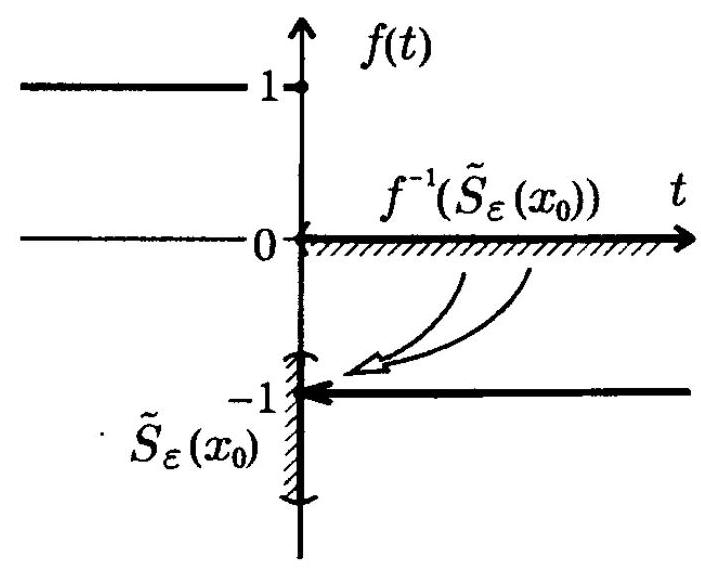
\includegraphics[max width=0.6\textwidth]{images/bo_d547okref24c73bgfch0_212_763_1601_701_569_0.jpg}
\end{center}
\hspace*{3em} 

Рис. Д7

Рассмотрим некоторые свойства измеримых функций, которые далее будем использовать. Класс непрерывных функций \(C\) вкладывается в класс измеримых функций \(L\), т.е. мы получили расширение класса всех непрерывных функций до класса всех измеримых функций.

Свойство 1. Функция \(f : {E}^{1} \rightarrow  {E}^{n}\) измерима на отрезке \(\left\lbrack  {{t}_{0},{t}_{1}}\right\rbrack\) тогда и только тогда, когда существует такая последовательность \({\mathbf{f}}_{k}\left( t\right)\) функций, непрерывных на отрезке \(\left\lbrack  {{t}_{0},{t}_{1}}\right\rbrack\), что при всех \(t \in \left\lbrack  {{t}_{0},{t}_{1}}\right\rbrack\) выполняется соотношение

\[
f\left( t\right)  = \mathop{\lim }\limits_{{k \rightarrow  \infty }}{f}_{k}\left( t\right)
\]

Свойство 2. Пусть \({\mathbf{f}}_{k} : {E}^{1} \rightarrow  {E}^{n}\) -- последовательность таких измеримых функций, что для каждого \(t\) последовательность \(\left\{  {{\mathbf{f}}_{k}\left( t\right) }\right\}\) сходится к значению \(\mathbf{f}\left( t\right)\). Тогда предельная функция \(\mathbf{f}\left( t\right)\) измерима.

Таким образом, пространство измеримых функций является замкнутым относительно поточечной сходимости.

Свойство 3. Если функция \(f : {E}^{1} \rightarrow  {E}^{n}\) измерима, а функция \(g : {E}^{n} \rightarrow  {E}^{m}\) -- непрерывна, то их суперпозиция \(\mathbf{g}\left( {\mathbf{f}\left( t\right) }\right)  : {E}^{1} \rightarrow  {E}^{m}\) будет функцией измеримой.

Свойство 4. Пусть \({\mathbf{f}}_{1}\left( t\right)\), \({\mathbf{f}}_{2}\left( t\right)\), \(\lambda \left( t\right)\) -- измеримые функции. Тогда функции \({\mathbf{f}}_{1}\left( t\right)  \pm  {\mathbf{f}}_{2}\left( t\right)\), \(\lambda \left( t\right) {\mathbf{f}}_{1}\left( t\right)\) и \(\frac{{\mathbf{f}}_{1}\left( t\right) }{\lambda \left( t\right) }\left( {\text{при }\lambda \left( t\right)  \neq  0}\right)\) также измеримы.

Функция \(\mathbf{f} : {E}^{1} \rightarrow  {E}^{n}\) называется простой, если она принимает не более чем счетное число значений \({x}_{1},{x}_{2},\ldots  \in  {E}^{n}\).

Свойство 5. Пусть функция \(f : {E}^{1} \rightarrow  {E}^{n}\) простая и \({\mathbf{x}}_{1},{\mathbf{x}}_{2},\ldots  \in  {E}^{n}\) есть множество ее значений. В таком случае функция \(f\left( t\right)\) измерима тогда и только тогда, когда измеримы все множества \({A}_{i} = \left\{  {t \in  {E}^{1} : f\left( t\right)  = {x}_{i}}\right\}\).

Свойство 6. Функция \(f : {E}^{1} \rightarrow  {E}^{n}\) измерима тогда и только тогда, когда она является равномерным пределом последовательности простых функций, т.е. существует такая последовательность \({\mathbf{f}}_{k}\left( t\right)\) простых измеримых функций, что \(\mathbf{f}\left( t\right)  = \mathop{\lim }\limits_{{k \rightarrow   + \infty }}{\mathbf{f}}_{k}\left( t\right)\) равномерно для всех \(t \in  {E}^{1}\).

\section*{Интеграл Лебега}

Оказывается, понятие интеграла можно распространить на класс измеримых функций. Сначала сделаем это для простых измеримых функций. Пусть заданы отрезок \(I = \left\lbrack  {{t}_{0},{t}_{1}}\right\rbrack   \subset  {E}^{1}\), простая измеримая функция \(f : I \rightarrow  {E}^{n}\) и множество ее значений \({x}_{1},{x}_{2},\ldots  \in  {E}^{n}\). Тогда по свойству 5 измеримых функций все множества \(\left\{  {t : {x}_{i} = f\left( t\right) }\right\}\) измеримы. Если ряд

\[
\mathop{\sum }\limits_{{i = 1}}^{\infty }\mu \left( \left\{  {t : f\left( t\right)  = {x}_{i}}\right\}  \right) {x}_{i}
\]

абсолютно сходится, то его сумму назовем интегралом Лебега от функции \(f\left( t\right)\) и обозначим \({\int }_{{t}_{0}}^{{t}_{1}}f\left( t\right) {dt}\) . Таким образом,

\[
{\int }_{{t}_{0}}^{{t}_{1}}\mathbf{f}\left( t\right) {dt} = \mathop{\sum }\limits_{{i = 1}}^{\infty }\mu \left( \left\{  {t : \mathbf{f}\left( t\right)  = {\mathbf{x}}_{i}}\right\}  \right) {\mathbf{x}}_{i}.
\]

Пример 2. Пусть функция \(f : {E}^{1} \rightarrow  {E}^{1}\) кусочно постоянна на отрезке \(\left\lbrack  {0,l}\right\rbrack\), где \(l\) -- целое число, и задана следующим образом: \(f\left( t\right)  = {f}_{i}\) при \(i \leq  t < i + 1\;\left( {i = 0,1,\ldots ,l - 1}\right)\) (рис. Д8). Среди чисел \({f}_{i}\) могут быть и совпадающие. Обозначим через \({x}_{j},j = 0,1,\ldots ,m \leq  l - 1\) набор всех различных чисел из \(\left\{  {f}_{i}\right\}\). Интеграл Лебега от этой функции имеет вид

\[
{\int }_{0}^{l}f\left( t\right) {dt} = \mathop{\sum }\limits_{{j = 0}}^{m}\mu \left( \left\{  {t : f\left( t\right)  = {x}_{j}}\right\}  \right) {x}_{j}.
\]
 (Д.45)

Функция \(f\left( t\right)\) кусочно постоянна на отрезке \(\left\lbrack  {0,l}\right\rbrack\). Поэтому у функции \(f\left( t\right)\) существует обычный интеграл Римана. Он имеет вид

\[
{\int }_{0}^{l}f\left( t\right) {dt} = \mathop{\sum }\limits_{{i = 0}}^{{l - 1}}{f}_{i}
\]
 (Д.46)

и равен площади заштрихованной фигуры (рис. Д8). Ясно, что эти интегралы совпадают. Поясним, как вычисляется этот интеграл по Риману и по Лебегу. По Риману (см. формулу (Д.46)) необходимо просуммировать подряд все числа \({f}_{i}\), по Лебегу (см. формулу (Д.45)) -- найти общую длину \(\mu \left( \left\{  {t : f\left( t\right)  = {x}_{j}}\right\}  \right)\) отрезков, где функция \(f\left( t\right)\) принимает одно и то же значение \({x}_{j}\), умножить эту длину на значение \({x}_{j}\) и все просуммировать. Различие между этими интегралами наглядно иллюстрирует сравнение, которое принадлежит Лебегу: у нас имеется мешок денег и нужно найти их общую сумму. По Риману надо вынимать из мешка по одной монете и, складывая цифры, написанные на монетах, найти общую сумму, по Лебегу -- сначала разложить все монеты на кучки из монет одного достоинства, найти сумму в каждой кучке и все просуммировать.

\begin{center}
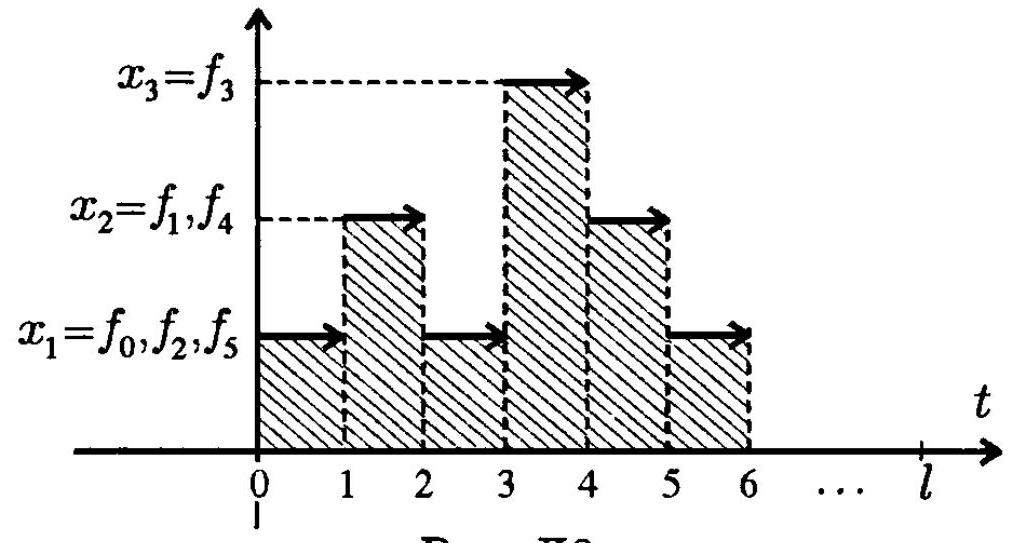
\includegraphics[max width=0.9\textwidth]{images/bo_d547okref24c73bgfch0_215_229_0_1013_543_0.jpg}
\end{center}
\hspace*{3em} 

Рис. Д8

\iffalse
Пусть теперь задана произвольная измеримая функция \(\mathbf{f}\) : \(I \rightarrow  {E}^{n}\) . Тогда по свойству б измеримых функций существует последовательность \({f}_{k}\left( t\right)\) простых измеримых функций такая, что для всех \(t \in  I\) выполнено соотношение \(\mathop{\lim }\limits_{{k \rightarrow  \infty }}{f}_{k}\left( t\right)  = f\left( t\right)\) . Ec- ли существует предел \(\mathop{\lim }\limits_{{k \rightarrow  \infty }}{\int }_{{t}_{0}}^{{t}_{1}}{f}_{k}\left( t\right) {dt}\) ,то он называется интег- ралом Лебега от функции \(f\left( t\right)\) иобозначается через \({\int }_{{t}_{0}}^{{t}_{1}}f\left( t\right) {dt}\) . Таким образом, имеем

\[
{\int }_{{t}_{0}}^{{t}_{1}}f\left( t\right) {dt} = \mathop{\lim }\limits_{{k \rightarrow  \infty }}{\int }_{{t}_{0}}^{{t}_{1}}{f}_{k}\left( t\right) {dt}
\]

Конечно, нужно доказать корректность такого определения ин- теграла Лебега, т.е. доказать, что интеграл Лебега от функции \(f\left( t\right)\) не зависит от выбора последовательности простых функ- ций \({f}_{k}\left( t\right)\) .

Рассмотрим некоторые свойства интеграла Лебега.

Свойство 1. Если функция f : I → Е" интегрируема по Риману, то она также интегрируема по Лебегу, и эти ин- тегралы совпадают.

Таким образом, интеграл Лебега является расширением ин- теграла Римана на измеримые функции.

Свойство 2. \({\Phi y} \text{ н } {\kappa yuA}\) f : \(I \rightarrow  {E}^{n}\) интегрируема по Ле- бегу тогда и только тогда, когда функция f(t) измерима и \(\parallel \mathbf{f}\left( t\right) \parallel  \leq  k\left( t\right)\) для всех t ∈ \(I\) ,где k : \(I \rightarrow  {E}^{1} - {c\kappa }\) алярная функция, интегрируемая по Лебегу.

Заметим, что ограниченная функция \(f : I \rightarrow  {E}^{n}\) интегри- руема по Риману тогда и только тогда, когда она непрерывна почти всюду на отрезке \(I\) .

Для интеграла Лебега выполняются все обычные свойства интеграла Римана. Приведем здесь лишь часть из них.

Свойство 3. Если функции \(f,{f}_{1},{f}_{2} : {E}^{1} \rightarrow  {E}^{n}\) интегриру- емы и \(\lambda  -\) некоторое число, то справедливы соотношения

\[
{\int }_{{t}_{0}}^{{t}_{1}}\left\lbrack  {{\mathbf{f}}_{1}\left( t\right)  \pm  {\mathbf{f}}_{2}\left( t\right) }\right\rbrack  {dt} = {\int }_{{t}_{0}}^{{t}_{1}}{\mathbf{f}}_{1}\left( t\right) {dt} \pm  {\int }_{{t}_{0}}^{{t}_{1}}{\mathbf{f}}_{2}\left( t\right) {dt}
\]

\[
{\int }_{{t}_{0}}^{{t}_{1}}{\lambda f}\left( t\right) {dt} = \lambda {\int }_{{t}_{0}}^{{t}_{1}}f\left( t\right) {dt}
\]

\[
{\int }_{{t}_{0}}^{\tau }\mathbf{f}\left( t\right) {dt} + {\int }_{\tau }^{{t}_{1}}\mathbf{f}\left( t\right) {dt} = {\int }_{{t}_{0}}^{{t}_{1}}\mathbf{f}\left( t\right) {dt},\;\tau  \in  I,
\]

\[
\left\lVert \begin{array}{c} {{\int }_{{t}_{0}}^{{t}_{1}}f\left( t\right) {dt}} \end{array} \right\rVert \leq  {\int }_{{t}_{0}}^{{t}_{1}}\parallel f\left( t\right) \parallel {dt}.
\]

Свойство 4. Пусть функция \(f : I \rightarrow  {E}^{n}\) интегрируема и \(\tau  \in  I\) . Тогда интеграл

\[
\mathbf{g}\left( \tau \right)  = {\int }_{{t}_{0}}^{\tau }\mathbf{f}\left( t\right) {dt}
\]

непрерывно зависит от верхнего предела интегрирования τ, т.е. функция \(g : I \rightarrow  {E}^{n}\) непрерывна.

Приведем два свойства интеграла Лебега для случая \(n = 1\) .

Свойство 5. Если функция \(f : I \rightarrow  {E}^{1}\) интегрируема и \(f\left( t\right)  \geq  0,{\;\operatorname{mod}\;{\int }_{{t}_{0}}^{{t}_{1}}}f\left( t\right) {dt} \geq  0.\)

Свойство 6. Ecлu функция f : I → E' интегрируема, \(f\left( t\right)  \geq  {0u}{\int }_{{t}_{0}}^{{t}_{1}}f\left( t\right) {dt} = 0,{mo}\;{\phi y}m{\kappa {yux}}f\left( t\right)\) normu ecoò \(y\) на отрезке I равна нулю.

\fi

Пусть теперь задана произвольная измеримая функция \(\mathbf{f}\) : \(I \rightarrow  {E}^{n}\). Тогда по свойству 6 измеримых функций существует последовательность \({f}_{k}\left( t\right)\) простых измеримых функций такая, что для всех \(t \in  I\) выполнено соотношение \(\mathop{\lim }\limits_{{k \rightarrow  \infty }}{f}_{k}\left( t\right)  = f\left( t\right)\). Если существует предел \(\mathop{\lim }\limits_{{k \rightarrow  \infty }}{\int }_{{t}_{0}}^{{t}_{1}}{f}_{k}\left( t\right) {dt}\), то он называется интегралом Лебега от функции \(f\left( t\right)\) и обозначается через \({\int }_{{t}_{0}}^{{t}_{1}}f\left( t\right) {dt}\). Таким образом, имеем

\[
{\int }_{{t}_{0}}^{{t}_{1}}f\left( t\right) {dt} = \mathop{\lim }\limits_{{k \rightarrow  \infty }}{\int }_{{t}_{0}}^{{t}_{1}}{f}_{k}\left( t\right) {dt}
\]

Конечно, нужно доказать корректность такого определения интеграла Лебега, т.е. доказать, что интеграл Лебега от функции \(f\left( t\right)\) не зависит от выбора последовательности простых функций \({f}_{k}\left( t\right)\).

Рассмотрим некоторые свойства интеграла Лебега.

Свойство 1. Если функция \(f : I \rightarrow  {E}^{n}\) интегрируема по Риману, то она также интегрируема по Лебегу, и эти интегралы совпадают.

Таким образом, интеграл Лебега является расширением интеграла Римана на измеримые функции.

Свойство 2. Функция \(f : I \rightarrow  {E}^{n}\) интегрируема по Лебегу тогда и только тогда, когда функция \(f\left( t\right)\) измерима и \(\parallel \mathbf{f}\left( t\right) \parallel  \leq  k\left( t\right)\) для всех \(t \in  I\), где \(k : I \rightarrow  {E}^{1}\) есть скалярная функция, интегрируемая по Лебегу.

Заметим, что ограниченная функция \(f : I \rightarrow  {E}^{n}\) интегрируема по Риману тогда и только тогда, когда она непрерывна почти всюду на отрезке \(I\).

Для интеграла Лебега выполняются все обычные свойства интеграла Римана. Приведем здесь лишь часть из них.

Свойство 3. Если функции \(f,{f}_{1},{f}_{2} : {E}^{1} \rightarrow  {E}^{n}\) интегрируемы и \(\lambda\) есть некоторое число, то справедливы соотношения

\[
{\int }_{{t}_{0}}^{{t}_{1}}\left\lbrack  {{\mathbf{f}}_{1}\left( t\right)  \pm  {\mathbf{f}}_{2}\left( t\right) }\right\rbrack  {dt} = {\int }_{{t}_{0}}^{{t}_{1}}{\mathbf{f}}_{1}\left( t\right) {dt} \pm  {\int }_{{t}_{0}}^{{t}_{1}}{\mathbf{f}}_{2}\left( t\right) {dt}
\]

\[
{\int }_{{t}_{0}}^{{t}_{1}}{\lambda f}\left( t\right) {dt} = \lambda {\int }_{{t}_{0}}^{{t}_{1}}f\left( t\right) {dt}
\]

\[
{\int }_{{t}_{0}}^{\tau }\mathbf{f}\left( t\right) {dt} + {\int }_{\tau }^{{t}_{1}}\mathbf{f}\left( t\right) {dt} = {\int }_{{t}_{0}}^{{t}_{1}}\mathbf{f}\left( t\right) {dt},\;\tau  \in  I,
\]

\[
\left\lVert \begin{array}{c} {{\int }_{{t}_{0}}^{{t}_{1}}f\left( t\right) {dt}} \end{array} \right\rVert \leq  {\int }_{{t}_{0}}^{{t}_{1}}\parallel f\left( t\right) \parallel {dt}.
\]

Свойство 4. Пусть функция \(f : I \rightarrow  {E}^{n}\) интегрируема и \(\tau  \in  I\). Тогда интеграл

\[
\mathbf{g}\left( \tau \right)  = {\int }_{{t}_{0}}^{\tau }\mathbf{f}\left( t\right) {dt}
\]

непрерывно зависит от верхнего предела интегрирования \(\tau\), т.е. функция \(g : I \rightarrow  {E}^{n}\) непрерывна.

Приведем два свойства интеграла Лебега для случая \(n = 1\).

Свойство 5. Если функция \(f : I \rightarrow  {E}^{1}\) интегрируема и \(f\left( t\right)  \geq  0\), то \({\int }_{{t}_{0}}^{{t}_{1}}f\left( t\right) {dt} \geq  0\).

Свойство 6. Если функция \(f : I \rightarrow  {E}^{1}\) интегрируема, \(f\left( t\right)  \geq  0\) и \({\int }_{{t}_{0}}^{{t}_{1}}f\left( t\right) {dt} = 0\), то функция \(f\left( t\right)\) почти всюду на отрезке \(I\) равна нулю.

\section*{Д7. Многозначные отображения}
\iffalse

Многозначным отображением называется (см. лекцию 4) произвольная функция \(F : {E}^{1} \rightarrow  \Omega \left( {E}^{n}\right)\) ,т.е. функция \(F\left( t\right)\) , значения которой суть непустые компактные множества в про- странстве \({E}^{n}\) . Отображение \(F\left( t\right)\) назовем измеримым на отрезке \(I = \left\lbrack  {{t}_{0},{t}_{1}}\right\rbrack\) , ecли его опорная функция \(c\left( {F\left( t\right) ,\psi }\right)\) измерима по \(t\) на отрезке \(I\) для каждого фиксированного вектора ф ∈ E". Такое определение измеримости является очень общим, и широ- кий класс функций \(F\left( t\right)\) измерим в указанном смысле. Обычно в литературе по многозначным функциям измеримость опреде- ляют для более узкого класса отображений \(F\left( t\right)\) . Поскольку по опорной функции \(c\left( {F\left( t\right) ,\psi }\right)\) можно восстановить лишь выпук- лую оболочку conv \(F\left( t\right)\) ,данное определение измеримости накла- дывает ограничение на поведение лишь многозначной функции conv \(F : {E}^{1} \rightarrow  \Omega \left( {E}^{n}\right)\) и никак не отражает того, что происходит с той частью множества \(F\left( t\right)\) , которая лежит внутри conv \(F\left( t\right)\) . Тем не менее все приводимые ниже результаты справедливы для многозначных отображений \(F\left( t\right)\) ,измеримых в указанном смысле.

Любое непрерывное многозначное отображение \(F : {E}^{1} \rightarrow \; \rightarrow  \Omega \left( {E}^{n}\right)\) измеримо, поскольку его опорная функция \(c\left( {F\left( t\right) ,\psi }\right)\) непрерывна по \(t\) при каждом фиксированном \(\psi  \in  {E}^{n}\) (см. тео- рему 1 из лекции 4) и, следовательно, измерима.

Теорема 1 (теорема Филиппова). Если многозначное отображение \(F : {E}^{1} \rightarrow  \Omega \left( {E}^{n}\right)\) измеримо, то у него существует измеримая однозначная ветвь \(\mathbf{f}\left( t\right)  \in  F\left( t\right)\).

Доказательство. Пусть многозначное отображение F(t) измеримо, т.е. его опорная функция \(c\left( {F\left( t\right) ,\mathbf{\psi }}\right)\) измерима по \(t\) .

Зафиксируем произвольный вектор \({\mathbf{\psi }}_{0} \in  {E}^{n}\) и рассмотрим опорное множество \(\mathcal{U}\left( {F\left( t\right) ,{\mathbf{\psi }}_{0}}\right)\) . Его опорная функция \(c(\mathcal{U}(F\left( t\right)\) , мум) имеет вид (см. следствие из теоремы 1, раздел Д5)

\[
c\left( {\mathcal{U}\left( {F\left( t\right) ,{\psi }_{0}}\right) ,\psi }\right)  = {c}^{\prime }\left( {F\left( t\right) ,{\psi }_{0};\psi }\right) .
\]

\[
{c}^{\prime }\left( {\mathcal{U}\left( {F\left( t\right) ,{\psi }_{0}}\right) ;\psi }\right)  = \mathop{\lim }\limits_{{\alpha  \rightarrow  0}}\frac{c\left( {F\left( t\right) ,{\psi }_{0} + {\alpha \psi }}\right)  - c\left( {F\left( t\right) ,{\psi }_{0}}\right) }{\alpha }.
\]
 (Д.47)

Cледовательно, опорная функция \(c\left( {\mathcal{U}\left( {F\left( t\right) ,{\psi }_{0}}\right) ,\psi }\right)\) измерима по \(t\) как предел последовательности измеримых функций (см. свой- ство 2 измеримых функций, раздел Д6). Поскольку F(t) ∈ \(\in  \Omega \left( {E}^{n}\right)\) , то \(\mathcal{U}\left( {F\left( t\right) ,{\psi }_{0}}\right)  \in  \Omega \left( {E}^{n}\right)\) , т.е. опорное множество не- пусто и компактно. Далее, множество \(\mathcal{U}\left( {F\left( t\right) ,{\psi }_{0}}\right)\) содержится в гиперплоскости \({\mathbf{\Gamma }}_{{\mathbf{\psi }}_{\mathbf{0}}}\) , опорной к множеству F(t). Следовательно, его размерность не превосходит n - 1 (размерность множества \(F \subset  {E}^{n}\) равна размерности минимального линейного многооб- разия, содержащего множество F).

Будем теперь последовательно выбирать в качестве вектора \({\mathbf{\psi }}_{0}\) базисные векторы \({\mathbf{e}}_{1},\ldots ,{\mathbf{e}}_{n}\) пространства \({E}^{n}\) . Рассмотрим последовательность многозначных отображений

\[
{\mathcal{U}}_{1}\left( t\right)  = \mathcal{U}\left( {F\left( t\right) ,{e}_{1}}\right) ,{\mathcal{U}}_{2}\left( t\right)  = \mathcal{U}\left( {{\mathcal{U}}_{1}\left( t\right) ,{e}_{2}}\right) ,\ldots
\]

\[
\ldots ,{\mathcal{U}}_{n}\left( t\right)  = \mathcal{U}\left( {{\mathcal{U}}_{n - 1}\left( t\right) ,{e}_{n}}\right)
\]

Опорная функция \(c\left( {{\mathcal{U}}_{i}\left( t\right) ,\mathbf{\psi }}\right)\) каждого отображения \({\mathcal{U}}_{i}\left( t\right)\) из дан- ной последовательности измерима по t. Кроме того, для лю- бого \(t \in  {E}^{1}\) справедливо включение \({\mathcal{U}}_{i}\left( t\right)  \in  \Omega \left( {E}^{n}\right)\) и размер- ность множества \({\mathcal{U}}_{i}\left( t\right)\) не превосходит \(n - i\) ,поскольку это мно- жество лежит в пересечении i ортогональных гиперплоскостей \({\Gamma }_{{e}_{1}},\ldots ,{\Gamma }_{{e}_{i}}\) . Согласно определению опорного множества имеем последовательность включений

\[
{\mathcal{U}}_{n}\left( t\right)  \subset  {\mathcal{U}}_{n - 1}\left( t\right)  \subset  \ldots  \subset  {\mathcal{U}}_{1}\left( t\right)  \subset  F\left( t\right) .
\]

Поскольку размерность множества Йо, (н) не превосходит нуля и \({\mathcal{U}}_{n}\left( t\right)  \in  \Omega \left( {E}^{n}\right)\) , множество \({\mathcal{U}}_{n}\left( t\right)\) состоит из единственной точки \({u}_{n}\left( t\right)\) . Обозначим ее через \(f\left( t\right)\) , т.е. \(f\left( t\right)  = {u}_{n}\left( t\right)\) . Далее, опорная функция \(c\left( {{\mathcal{U}}_{n}\left( t\right) ,\psi }\right)  = \left\langle  {{\mathbf{u}}_{n}\left( t\right) ,\psi }\right\rangle   = \langle \mathbf{f}\left( t\right) ,\psi \rangle\) измерима по t для любого вектора \(\psi  \in  {E}^{n}\) . Отсюда следует, что сама функция \(f\left( t\right)  : {E}^{1} \rightarrow  {E}^{n}\) измерима. Действительно, если положить после- довательно \(\psi  = {e}_{1},\ldots ,{e}_{n}\) , то получим, что каждая координата \({f}_{i}\left( t\right)  = \left\langle  {\mathbf{f}\left( t\right) ,{\mathbf{e}}_{i}}\right\rangle\) y функции \(\mathbf{f}\left( t\right)\) измерима. Теперь сама функция

\[
f\left( t\right)  = {f}_{1}\left( t\right) {e}_{1} + \ldots  + {f}_{n}\left( t\right) {e}_{n}
\]

измерима как суперпозиция непрерывной и измеримых функ- ций (свойство 3 измеримых функций из раздела Д6). Поскольку \(f\left( t\right)  \in  F\left( t\right)\) при всех t ∈ \({E}^{1}\) , то \(f\left( t\right)\) есть измеримая однозначная ветвь отображения \(F\left( t\right)\) . Теорема доказана.

Следствие 1. Пусть F : \({E}^{1} \rightarrow  \Omega \left( {E}^{n}\right)  - {u3\text{ м }\text{ е }\text{ р }\text{ и }\text{ м }\text{ о }\text{ е }}\) многозначное отображение, \({\psi }_{0} \in  {E}^{n} - {\phi u\kappa cupo\text{ в }a}\) ный век- mop. Тогда отображение \(\mathcal{U}\left( {F\left( t\right) ,{\mathbf{\psi }}_{0}}\right) \;{u3}\) меримо и, следова- тельно, у него существует измеримая однозначная ветвь \(\mathbf{f}\left( t\right)  \in  \mathcal{U}\left( {F\left( t\right) ,{\mathbf{\psi }}_{0}}\right) .\)

Доказательство. Достаточно убедиться в том, что опор- ная функция \(c\left( {\mathcal{U}\left( {F\left( t\right) ,{\mathbf{\psi }}_{0}}\right) ,\mathbf{\psi }}\right)\) отображения \(\mathcal{U}\left( {F\left( t\right) ,{\mathbf{\psi }}_{0}}\right)\) измери- ма. А это было показано при доказательстве теоремы 1 (см. формулу (Д.47)).

Сформулируем еще одно совсем очевидное следствие в том виде, в каком оно будет использовано далее.

Следствие 2. Пусть многозначное отображение \(F : {E}^{1} \rightarrow  \Omega \left( {E}^{n}\right)\) непрерывно на отрезке \(I = \left\lbrack  {{t}_{0},{t}_{1}}\right\rbrack\). Тогда у него существует измеримая на этом отрезке однозначная ветвь \(f\left( t\right)  \in  F\left( t\right)\). Более того, если \(\psi \in S\) -- произвольный фиксированный вектор, то существует измеримая ветвь \(f\left( t\right)\) отображения \(\mathcal{U}\left( {F\left( t\right) ,\psi }\right)\), т.е. \(f\left( t\right)  \in  \mathcal{U}\left( {F\left( t\right) ,\psi }\right)\) при всех \(t \in I\).

Пусть \(I = \left\lbrack  {{t}_{0},{t}_{1}}\right\rbrack\) и задано некоторое многозначное отобра- жение \(F : I \rightarrow  \Omega \left( {E}^{n}\right)\) .

Определение 1. Интегралом от многозначного отобра- жения \(F\left( t\right)\) на отрезке I называется множество

\[
G = {\int }_{{t}_{0}}^{{t}_{1}}F\left( t\right) {dt} = \left\{  {{\int }_{{t}_{0}}^{{t}_{1}}\mathbf{f}\left( t\right) {dt} : \mathbf{f}\left( t\right)  \in  F\left( t\right) }\right\}  .
\]

Здесь в правой части интеграл Лебега берется по всем одно- значным ветвям отображения \(F\left( t\right)\) ,для которых он существует. Ясно, что \(G\) является подмножеством пространства E".

Теорема 2 (теорема Ляпунова). Пусть многозначное отображение \(F\left( t\right)\) измеримо и удовлетворяет оценке \(\left| {F\left( t\right) }\right|  \leq  k\left( t\right)\), где \(k\left( t\right)\) -- скалярная функция, интегрируемая по Лебегу на отрезке \(I = \left\lbrack  {{t}_{0},{t}_{1}}\right\rbrack\). Тогда интеграл от этого многозначного отображения является непустым компактным множеством в пространстве \({E}^{n}\), т.е.

\[
G = {\int }_{{t}_{0}}^{{t}_{1}}F\left( t\right) {dt} \in  \Omega \left( {E}^{n}\right) .
\]

Более того, множество G выпукло.

Эта теорема (как теорема о векторных мерах) была впервые доказана в работе [5]. В последующих работах (см., в частности, работы [7], [8]) ее доказательство было значительно упрощено.

Докажем предварительно три леммы, при этом будем всегда считать, что выполнены предположения теоремы 2.

Лемма 1. Множество G непусто и ограничено.

Доказательство. Покажем, что множество G непусто. Действительно, согласно теореме 1 существует хотя бы одна измеримая ветвь \(f\left( t\right)\) у многозначного отображения \(F\left( t\right)\) . Далее, очевидно, имеем неравенство

\[
\parallel f\left( t\right) \parallel  \leq  \left| {F\left( t\right) }\right|  \leq  k\left( t\right) . \tag{II.48}
\]

Таким образом, согласно свойству 2 интеграла Лебега (см. раз- дел Д6) любая измеримая ветвь \(f\left( t\right)\) интегрируема и \({\int }_{{t}_{0}}^{{t}_{1}}f\left( t\right) {dt} \in \; \in  G\) ,т.е. множество \(G\) непусто. Покажем,что множество G ограничено. Действительно, пусть g ∈ \(G\) . Тогда g \(= {\int }_{{t}_{0}}^{{t}_{1}}f\left( t\right) {dt}\) , где \(\mathbf{f}\left( t\right)\) — некоторая ветвь из многозначного отображения \(F\left( t\right)\) . В силу свойства 3 интеграла Лебегаи соотнощения \(\left( {\text{ Д }.48}\right)\) имеем

\[
\parallel \mathbf{g}\parallel  = \left\lVert \begin{array}{c} {\mathop{\int }\limits_{{t}_{0}}^{{t}_{1}}\mathbf{f}\left( t\right) {dt}} \end{array} \right\rVert \leq  \mathop{\int }\limits_{{t}_{0}}^{{t}_{1}}\parallel \mathbf{f}\left( t\right) \parallel {dt} \leq  \mathop{\int }\limits_{{t}_{0}}^{{t}_{1}}k\left( t\right) {dt} = k.
\]

Таким образом, \(G \subset  {S}_{k}\left( \mathbf{0}\right)\) , т.е. множество \(G\) ограничено. Лем- ма 1 доказана.

Лемма 2. Для интеграла от многозначного отображения G можно определить опорную функцию

\[
c\left( {G,\psi }\right)  = \mathop{\sup }\limits_{{g \in  G}}\langle g,\psi \rangle .
\]
 (Д.49)

Максимум в этом выражении всегда достигается. Более то-

\[
c\left( {{\int }_{{t}_{0}}^{{t}_{1}}F\left( t\right) {dt},\psi }\right)  = {\int }_{{t}_{0}}^{{t}_{1}}c\left( {F\left( t\right) ,\psi }\right) {dt}.
\]
 (Д.50)

Доказательство. Заметим, что интеграл в правой час- ти равенства (Д.50) существует, поскольку опорная функция \(c\left( {F\left( t\right) ,\psi }\right)\) измерима по \(t\) и удовлетворяет оценке

\[
\left| {c\left( {F\left( t\right) ,\psi }\right) }\right|  \leq  \left| {F\left( t\right) }\right|  \cdot  \parallel \psi \parallel  \leq  k\left( t\right) \parallel \psi \parallel .
\]

Зафиксируем произвольный вектор \(\psi  \in  {E}^{n}\) . IIycть \(g \in  G\) . Согласно определению интеграла существует измеримая одно- значная ветвь \(f\left( t\right)  \in  F\left( t\right)\) такая,что \(g = {\int }_{{t}_{0}}^{{t}_{1}}f\left( t\right) {dt}\) . Согласно следствию из свойства 6 опорных функций (см. лекцию 3) имеем неравенство

\[
\langle f\left( t\right) ,\psi \rangle  \leq  c\left( {F\left( t\right) ,\psi }\right) .
\]
 (Д.51)

В силу следствия 1 из теоремы 1 у отображения \(\mathcal{U}\left( {F\left( t\right) ,\mathbf{\psi }}\right)\) cy- ществует измеримая однозначная ветвь \({\mathbf{f}}^{ * }\left( t\right)\) . Согласно оценке \(\left| {F\left( t\right) }\right|  \leq  k\left( t\right)\) эта ветвь интегрируема на отрезке I. По определе- нию опорного множества имеем равенство

\[
c\left( {F\left( t\right) ,\psi }\right)  = \left\langle  {{\mathbf{f}}^{ * }\left( t\right) ,\psi }\right\rangle  .
\]
 (Д.52)

Таким образом, используя свойство интеграла Лебега, из формул (Д.51) и (Д.52) получаем цепочку соотношений

\[
c\left( {G,\psi }\right)  = \mathop{\sup }\limits_{{g \in  G}}\langle g,\psi \rangle  = \mathop{\sup }\limits_{{f\left( t\right)  \in  F\left( t\right) }}{\int }_{{t}_{0}}^{{t}_{1}}\langle f\left( t\right) ,\psi \rangle {dt} \leq
\]

\[
\leq  {\int }_{{t}_{0}}^{{t}_{1}}c\left( {F\left( t\right) ,\psi }\right) {dt} = {\int }_{{t}_{0}}^{{t}_{1}}\left\langle  {{f}^{ * }\left( t\right) ,\psi }\right\rangle  {dt} \leq  c\left( {G,\psi }\right) .
\]

Следовательно, во всех неравенствах достигается равенство, т.е. справедлива формула (Д.50), и супремум можно заменить на максимум. Этот максимум достигается в точке

\[
{g}^{ * } = {\int }_{{t}_{0}}^{{t}_{1}}{f}^{ * }\left( t\right) {dt}
\]

Лемма доказана.

\fi

Многозначным отображением называется (см. лекцию 4) произвольная функция \(F : {E}^{1} \rightarrow  \Omega \left( {E}^{n}\right)\), т.е. функция \(F\left( t\right)\), значения которой суть непустые компактные множества в пространстве \({E}^{n}\). Отображение \(F\left( t\right)\) назовем измеримым на отрезке \(I = \left\lbrack  {{t}_{0},{t}_{1}}\right\rbrack\), если его опорная функция \(c\left( {F\left( t\right) ,\psi }\right)\) измерима по \(t\) на отрезке \(I\) для каждого фиксированного вектора \(\psi \in {E}^{n}\). Такое определение измеримости является очень общим; тем не менее все приводимые ниже результаты справедливы для многозначных отображений \(F\left( t\right)\), измеримых в указанном смысле.

Любое непрерывное многозначное отображение \(F : {E}^{1} \rightarrow  \Omega \left( {E}^{n}\right)\) измеримо, поскольку его опорная функция \(c\left( {F\left( t\right) ,\psi }\right)\) непрерывна по \(t\) при каждом фиксированном \(\psi \in {E}^{n}\) (см. теорему 1 из лекции 4) и, следовательно, измерима.

Теорема 1 (теорема Филиппова). Если многозначное отображение \(F : {E}^{1} \rightarrow  \Omega \left( {E}^{n}\right)\) измеримо, то у него существует измеримая однозначная ветвь \(\mathbf{f}\left( t\right) \in F\left( t\right)\).

Доказательство. Пусть многозначное отображение \(F\left( t\right)\) измеримо, т.е. его опорная функция \(c\left( {F\left( t\right) ,\mathbf{\psi }}\right)\) измерима по \(t\).

Зафиксируем произвольный вектор \({\mathbf{\psi }}_{0} \in {E}^{n}\) и рассмотрим опорное множество \(\mathcal{U}\left( {F\left( t\right) ,{\mathbf{\psi }}_{0}}\right)\). Его опорная функция имеет вид (см. следствие из теоремы 1, раздел Д5)

\[
c\left( {\mathcal{U}\left( {F\left( t\right) ,{\psi }_{0}}\right) ,\psi }\right) = {c}^{\prime }\left( {F\left( t\right) ,{\psi }_{0};\psi }\right),
\]

\[
{c}^{\prime }\left( {F\left( t\right) ,{\psi }_{0};\psi }\right) = \mathop{\lim }\limits_{{\alpha \rightarrow 0}}\frac{c\left( {F\left( t\right) ,{\psi }_{0} + {\alpha \psi }}\right) - c\left( {F\left( t\right) ,{\psi }_{0}}\right)}{\alpha}.
\]
 (Д.47)

Следовательно, опорная функция \(c\left( {\mathcal{U}\left( {F\left( t\right) ,{\psi }_{0}}\right) ,\psi }\right)\) измерима по \(t\) как предел последовательности измеримых функций (см. свойство 2 измеримых функций, раздел Д6). Поскольку \(F\left( t\right) \in \Omega \left( {E}^{n}\right)\), то \(\mathcal{U}\left( {F\left( t\right) ,{\psi }_{0}}\right) \in \Omega \left( {E}^{n}\right)\), т.е. опорное множество непусто и компактно. Далее, это множество содержится в гиперплоскости \({\mathbf{\Gamma }}_{{\mathbf{\psi }}_{\mathbf{0}}}\), опорной к множеству \(F\left( t\right)\). Следовательно, его размерность не превосходит \(n - 1\).

Будем теперь последовательно выбирать в качестве вектора \({\mathbf{\psi }}_{0}\) базисные векторы \({\mathbf{e}}_{1},\ldots,{\mathbf{e}}_{n}\) пространства \({E}^{n}\). Рассмотрим последовательность многозначных отображений

\[
{\mathcal{U}}_{1}\left( t\right) = \mathcal{U}\left( {F\left( t\right) ,{e}_{1}}\right),\quad
{\mathcal{U}}_{2}\left( t\right) = \mathcal{U}\left( {{\mathcal{U}}_{1}\left( t\right) ,{e}_{2}}\right),\ldots,
\]

\[
{\mathcal{U}}_{n}\left( t\right) = \mathcal{U}\left( {{\mathcal{U}}_{n - 1}\left( t\right) ,{e}_{n}}\right).
\]

Опорная функция каждого отображения \({\mathcal{U}}_{i}\left( t\right)\) измерима по \(t\). Кроме того, для любого \(t\) справедливо включение \({\mathcal{U}}_{i}\left( t\right) \in \Omega \left( {E}^{n}\right)\), и размерность множества \({\mathcal{U}}_{i}\left( t\right)\) не превосходит \(n - i\), поскольку это множество лежит в пересечении \(i\) ортогональных гиперплоскостей. Согласно определению опорного множества имеем последовательность включений

\[
{\mathcal{U}}_{n}\left( t\right) \subset {\mathcal{U}}_{n - 1}\left( t\right) \subset \ldots \subset {\mathcal{U}}_{1}\left( t\right) \subset F\left( t\right).
\]

Поскольку размерность множества \({\mathcal{U}}_{n}\left( t\right)\) не превосходит нуля и \({\mathcal{U}}_{n}\left( t\right) \in \Omega \left( {E}^{n}\right)\), множество \({\mathcal{U}}_{n}\left( t\right)\) состоит из единственной точки \({u}_{n}\left( t\right)\). Обозначим ее через \(f\left( t\right)\). Тогда \(f\left( t\right)\) измерима, так как для любого \(\psi \in {E}^{n}\) функция
\[
c\left( {{\mathcal{U}}_{n}\left( t\right) ,\psi }\right) = \left\langle {{\mathbf{u}}_{n}\left( t\right),\psi}\right\rangle = \langle \mathbf{f}\left( t\right),\psi\rangle
\]
измерима по \(t\), а значит измеримы все координаты \(\mathbf{f}\left( t\right)\). Поскольку \(f\left( t\right) \in F\left( t\right)\) при всех \(t \in {E}^{1}\), то \(f\left( t\right)\) есть измеримая однозначная ветвь отображения \(F\left( t\right)\). Теорема доказана.

Следствие 1. Пусть \(F : {E}^{1} \rightarrow \Omega \left( {E}^{n}\right)\) -- измеримое многозначное отображение, \({\psi }_{0} \in {E}^{n}\) -- фиксированный вектор. Тогда отображение \(\mathcal{U}\left( {F\left( t\right),{\mathbf{\psi }}_{0}}\right)\) измеримо и, следовательно, у него существует измеримая однозначная ветвь \(\mathbf{f}\left( t\right) \in \mathcal{U}\left( {F\left( t\right),{\mathbf{\psi }}_{0}}\right)\).

Доказательство. Достаточно убедиться в том, что опорная функция \(c\left( {\mathcal{U}\left( {F\left( t\right),{\mathbf{\psi }}_{0}}\right),\mathbf{\psi }}\right)\) отображения \(\mathcal{U}\left( {F\left( t\right),{\mathbf{\psi }}_{0}}\right)\) измерима. А это было показано при доказательстве теоремы 1 (см. формулу (Д.47)).

Следствие 2. Пусть многозначное отображение \(F : {E}^{1} \rightarrow \Omega \left( {E}^{n}\right)\) непрерывно на отрезке \(I = \left\lbrack {{t}_{0},{t}_{1}}\right\rbrack\). Тогда у него существует измеримая на этом отрезке однозначная ветвь \(f\left( t\right) \in F\left( t\right)\). Более того, если \(\psi \in S\) -- произвольный фиксированный вектор, то существует измеримая ветвь \(f\left( t\right)\) отображения \(\mathcal{U}\left( {F\left( t\right),\psi}\right)\), т.е. \(f\left( t\right) \in \mathcal{U}\left( {F\left( t\right),\psi}\right)\) при всех \(t \in I\).

Пусть \(I = \left\lbrack {{t}_{0},{t}_{1}}\right\rbrack\) и задано некоторое многозначное отображение \(F : I \rightarrow \Omega \left( {E}^{n}\right)\).

Определение 1. Интегралом от многозначного отображения \(F\left( t\right)\) на отрезке \(I\) называется множество

\[
G = {\int }_{{t}_{0}}^{{t}_{1}}F\left( t\right) {dt} =
\left\{ {{\int }_{{t}_{0}}^{{t}_{1}}\mathbf{f}\left( t\right) {dt} : \mathbf{f}\left( t\right) \in F\left( t\right)}\right\}.
\]

Здесь в правой части интеграл Лебега берется по всем однозначным ветвям отображения \(F\left( t\right)\), для которых он существует. Ясно, что \(G\) является подмножеством пространства \({E}^{n}\).

Теорема 2 (теорема Ляпунова). Пусть многозначное отображение \(F\left( t\right)\) измеримо и удовлетворяет оценке \(\left| {F\left( t\right)}\right| \leq k\left( t\right)\), где \(k\left( t\right)\) -- скалярная функция, интегрируемая по Лебегу на отрезке \(I = \left\lbrack {{t}_{0},{t}_{1}}\right\rbrack\). Тогда интеграл от этого многозначного отображения является непустым компактным множеством в пространстве \({E}^{n}\), т.е.

\[
G = {\int }_{{t}_{0}}^{{t}_{1}}F\left( t\right) {dt} \in \Omega \left( {E}^{n}\right).
\]

Более того, множество \(G\) выпукло.

Эта теорема (как теорема о векторных мерах) была впервые доказана в работе [5]. В последующих работах (см., в частности, работы [7], [8]) ее доказательство было значительно упрощено.

Докажем предварительно три леммы, при этом будем всегда считать, что выполнены предположения теоремы 2.

Лемма 1. Множество \(G\) непусто и ограничено.

Доказательство. Покажем, что множество \(G\) непусто. Действительно, согласно теореме 1 существует хотя бы одна измеримая ветвь \(f\left( t\right)\) у многозначного отображения \(F\left( t\right)\). Далее, очевидно, имеем неравенство

\[
\parallel f\left( t\right) \parallel \leq \left| {F\left( t\right)}\right| \leq k\left( t\right). \tag{Д.48}
\]

Таким образом, согласно свойству 2 интеграла Лебега (см. раздел Д6) любая измеримая ветвь \(f\left( t\right)\) интегрируема и \({\int }_{{t}_{0}}^{{t}_{1}}f\left( t\right) {dt} \in G\), т.е. множество \(G\) непусто. Покажем, что множество \(G\) ограничено. Действительно, пусть \(\mathbf{g} \in G\). Тогда \(\mathbf{g} = {\int }_{{t}_{0}}^{{t}_{1}}f\left( t\right) {dt}\), где \(\mathbf{f}\left( t\right)\) -- некоторая ветвь из многозначного отображения \(F\left( t\right)\). В силу свойства 3 интеграла Лебега и соотношения \((Д.48)\) имеем

\[
\parallel \mathbf{g}\parallel =
\left\lVert \begin{array}{c} {\mathop{\int }\limits_{{t}_{0}}^{{t}_{1}}\mathbf{f}\left( t\right) {dt}} \end{array} \right\rVert
\leq \mathop{\int }\limits_{{t}_{0}}^{{t}_{1}}\parallel \mathbf{f}\left( t\right) \parallel {dt}
\leq \mathop{\int }\limits_{{t}_{0}}^{{t}_{1}}k\left( t\right) {dt} = \kappa .
\]

Таким образом, \(G \subset {S}_{\kappa}\left( \mathbf{0}\right)\), т.е. множество \(G\) ограничено. Лемма 1 доказана.

Лемма 2. Для интеграла от многозначного отображения \(G\) можно определить опорную функцию

\[
c\left( {G,\psi}\right) = \mathop{\sup }\limits_{{g \in G}}\langle g,\psi\rangle . \tag{Д.49}
\]

Максимум в этом выражении всегда достигается. Более того, имеет место равенство

\[
c\left( {{\int }_{{t}_{0}}^{{t}_{1}}F\left( t\right) {dt},\psi}\right)
= {\int }_{{t}_{0}}^{{t}_{1}}c\left( {F\left( t\right),\psi}\right) {dt}. \tag{Д.50}
\]

Доказательство. Заметим, что интеграл в правой части равенства \((Д.50)\) существует, поскольку опорная функция \(c\left( {F\left( t\right),\psi}\right)\) измерима по \(t\) и удовлетворяет оценке

\[
\left| {c\left( {F\left( t\right),\psi}\right)}\right| \leq \left| {F\left( t\right)}\right|\cdot\parallel\psi\parallel \leq k\left( t\right)\parallel\psi\parallel .
\]

Зафиксируем произвольный вектор \(\psi \in {E}^{n}\). Пусть \(g \in G\). Согласно определению интеграла существует измеримая однозначная ветвь \(f\left( t\right) \in F\left( t\right)\) такая, что \(g = {\int }_{{t}_{0}}^{{t}_{1}}f\left( t\right) {dt}\). Согласно следствию из свойства 6 опорных функций (см. лекцию 3) имеем неравенство

\[
\langle f\left( t\right),\psi\rangle \leq c\left( {F\left( t\right),\psi}\right). \tag{Д.51}
\]

В силу следствия 1 из теоремы 1 у отображения \(\mathcal{U}\left( {F\left( t\right),\mathbf{\psi}}\right)\) существует измеримая однозначная ветвь \({\mathbf{f}}^{ *}\left( t\right)\). Согласно оценке \(\left| {F\left( t\right)}\right| \leq k\left( t\right)\) эта ветвь интегрируема на отрезке \(I\). По определению опорного множества имеем равенство

\[
c\left( {F\left( t\right),\psi}\right) = \left\langle {{\mathbf{f}}^{ *}\left( t\right),\psi}\right\rangle . \tag{Д.52}
\]

Таким образом, используя свойство интеграла Лебега, из формул \((Д.51)\) и \((Д.52)\) получаем цепочку соотношений

\[
c\left( {G,\psi}\right) = \mathop{\sup }\limits_{{g \in G}}\langle g,\psi\rangle
= \mathop{\sup }\limits_{{f\left( t\right) \in F\left( t\right)}}{\int }_{{t}_{0}}^{{t}_{1}}\langle f\left( t\right),\psi\rangle {dt} \leq
\]

\[
\leq {\int }_{{t}_{0}}^{{t}_{1}}c\left( {F\left( t\right),\psi}\right) {dt}
= {\int }_{{t}_{0}}^{{t}_{1}}\left\langle {{f}^{ *}\left( t\right),\psi}\right\rangle {dt}
\leq c\left( {G,\psi}\right).
\]

Следовательно, во всех неравенствах достигается равенство, т.е. справедлива формула \((Д.50)\), и супремум можно заменить на максимум. Этот максимум достигается в точке

\[
{g}^{ *} = {\int }_{{t}_{0}}^{{t}_{1}}{f}^{ *}\left( t\right) {dt}.
\]

Лемма доказана.

\iffalse

Лемма 3. Пусть \(\psi \in {E}^{n}\) -- произвольный фиксированный вектор. Тогда справедливо равенство

\[
\mathcal{U}\left( {G,\psi }\right)  = {\int }_{{t}_{0}}^{{t}_{1}}\mathcal{U}\left( {F\left( t\right) ,\psi }\right) {dt} \tag{II.53}
\]

Показательство. Пусть до € И( G, ψ). Это означает, что \({g}_{0} \in  G\) и для всех g ∈ \(G\) выполняется неравенство

\[
\langle \mathbf{g},\mathbf{\psi }\rangle  \leq  \left\langle  {{\mathbf{g}}_{0},\mathbf{\psi }}\right\rangle  .
\]
 (Д.54)

Для точки \({g}_{0} \in  G\) имеем представление \({g}_{0} = {\int }_{{t}_{0}}^{{t}_{1}}{f}_{0}\left( t\right) {dt}\) ,где \({\mathbf{f}}_{0}\left( t\right)  -\) интегрируемая ветвь отображения \(F\left( t\right)\) . Согласно след- ствию 1 из теоремы 1 у отображения \(\mathcal{U}\left( {F\left( t\right) ,\psi }\right)\) существует измеримая однозначная ветвь f*6) и для нее справедливо ра- венство (Д.54). Подставим точку

\[
g = {g}^{ * } = {\int }_{{t}_{0}}^{{t}_{1}}{f}^{ * }\left( t\right) {dt} \in  G
\]

в неравенство (Д.54), получим тогда соотношение

\[
{\int }_{{t}_{0}}^{{t}_{1}}c\left( {F\left( t\right) ,\psi }\right) {dt} = \left\langle  {{\int }_{{t}_{0}}^{{t}_{1}}{f}^{ * }\left( t\right) {dt},\psi }\right\rangle   \leq
\]

\[
\leq  \left\langle  {{\int }_{{t}_{0}}^{{t}_{1}}{f}_{0}\left( t\right) {dt},\psi }\right\rangle   = {\int }_{{t}_{0}}^{{t}_{1}}\left\langle  {{f}_{0}\left( t\right) ,\psi }\right\rangle  {dt}.
\]

Таким образом, справедливо неравенство

\[
{\int }_{{t}_{0}}^{{t}_{1}}\left\lbrack  {c\left( {F\left( t\right) ,\psi }\right)  - \left\langle  {{f}_{0}\left( t\right) ,\psi }\right\rangle  }\right\rbrack  {dt} \leq  0,
\]

при этом подынтегральная функция неотрицательна в силу включения \({\mathbf{f}}_{0}\left( t\right)  \in  \bar{F}\left( t\right)\) . Согласно свойствам интеграла Лебега получаем равенство

\[
c\left( {F\left( t\right) ,\psi }\right)  - \left\langle  {{\mathbf{f}}_{0}\left( t\right) ,\psi }\right\rangle   = 0
\]
 (Д.55)

для почти всех t ∈ \(\left\lbrack  {{t}_{0},{t}_{1}}\right\rbrack\) , т.е. \({\mathbf{f}}_{0}\left( t\right)  \in  \mathcal{U}\left( {F\left( t\right) ,\mathbf{\psi }}\right)\) , и, следователь- но, имеем включение

\[
{g}_{0} \in  {\int }_{{t}_{0}}^{{t}_{1}}\mathcal{U}\left( {F\left( t\right) ,\psi }\right) {dt}
\]
 (Д.56)

Пусть теперь точка \({g}_{0}\) удовлетворяет включению (Д.56). Тогда \({\mathbf{g}}_{0} = {\int }_{{t}_{0}}^{{t}_{1}}{\mathbf{f}}_{0}\left( t\right) {dt}\) ,и ветвь \({\mathbf{f}}_{0}\left( t\right)  \in  \mathcal{U}\left( {F\left( t\right) ,\mathbf{\psi }}\right)\) удовлетворяет ра- венству (II.55). Следовательно, для произвольной точки g ∈ G выполняется соотношение

\[
\left\langle  {\mathbf{g} - {\mathbf{g}}_{0},\mathbf{\psi }}\right\rangle   = {\int }_{{t}_{0}}^{{t}_{1}}\left\lbrack  {\langle \mathbf{f}\left( t\right) ,\mathbf{\psi }\rangle  - c\left( {F\left( t\right) ,\mathbf{\psi }}\right) }\right\rbrack  {dt} \leq  0,
\]

так как подынтегральная функция неположительна в силу включения \(f\left( t\right)  \in  F\left( t\right)\) , т.е. выполнено неравенство (Д.54). Ta- ким образом, справедливо включение \({\mathbf{g}}_{0} \in  \mathcal{U}\left( {G,\mathbf{\psi }}\right)\) . Tem самым доказано равенство множеств в соотношении (Д.53).

При доказательстве теоремы 2 потребуется понятие размер- ности непустого множества A ⊂ E".

Определение 2. Размерностью dim A непустого множес- тва А называется размерность минимального линейного мно- гообразия L, содержащего множество А.

Так, размерность одной точки всегда равна 0, размерность любого отрезка в пространстве E" равна 1, размерность дуги окружности на плоскости \({E}^{2}\) равна 2, размерность множества с непустой внутренностью в \(E^n\) всегда равна размерности про- странства n. Если О ∈ A, то линейное многообразие L будет подпространством. Если замкнуть множество A, то его размер- ность не изменится, поскольку из включения \(A \subset  L\) следует включение \(\bar{A} \subset  L\) в силу замкнутости пространства L. Если при этом взять еще выпуклую оболочку множества A, то его раз- мерность также не изменится, поскольку из включения \(\bar{A} \subset  L\) следует включение conv \(\bar{A} \subset  L\) в силу выпуклости подпростран- ства L.

Доказательство теоремы 2. По лемме 1 интеграл G является множеством непустым и ограниченным. Нам остает- ся только доказать, что это множество замкнуто и выпукло. Отметим здесь, что при доказательстве лемм 1—3 мы нигде не пользовались замкнутостью и выпуклостью множества G. Заметим, что в лекции 5 порядок изложения результатов был другим.

При замыкании множества G его опорная функция не изме- нится, т.е. при всех у ее тер справедливо равенство

\[
c\left( {\bar{G},\psi }\right)  = c\left( {G,\psi }\right) .
\]
 (Д.57)

Действительно, в силу включения \(G \subset  \bar{G}\) всегда справедливо неравенство

\[
c\left( {G,\psi }\right)  \leq  c\left( {\bar{G},\psi }\right) .
\]
 (Д.58)

C другой стороны, если g ∈ G, то существует такая последова- тельность точек \({\mathbf{g}}_{k} \in  G\) , которая сходится к точке \({\mathbf{g}}_{0}\) . Для всех точек \({g}_{k} \in  G\) выполняется неравенство

\[
\left\langle  {{\mathbf{g}}_{k},\psi }\right\rangle   \leq  c\left( {G,\psi }\right) .
\]

Переходя в этом неравенстве к пределу при \(k \rightarrow  \infty\) ,получим соотношение

\[
\langle \mathbf{g},\mathbf{\psi }\rangle  \leq  c\left( {G,\mathbf{\psi }}\right) ,
\]

следовательно, выполняется неравенство

\[
c\left( {\bar{G},\psi }\right)  = \mathop{\max }\limits_{{\mathbf{g} \in  \bar{G}}}\langle \mathbf{g},\psi \rangle  \leq  c\left( {G,\psi }\right) .
\]

Таким образом, получаем с учетом неравенства (II.58) равенст- во (II.57).

Поскольку при переходе от множества к его выпуклой обо- лочке опорная функция не изменится (см. свойство 7 опорных функций, лекция 3), из формулы (Д.57) и леммы 2 получаем равенство

\[
c\left( {\operatorname{conv}\bar{G},\psi }\right)  = c\left( {G,\psi }\right)  = {\int }_{{t}_{0}}^{{t}_{1}}c\left( {F\left( t\right) ,\psi }\right) {dt}.
\]
 (Д.59)

Доказательство замкнутости и выпуклости множества G бу- дем проводить по индукции, причем индукцию будем проводить по размерности множества G, т.е. по числам k = dim G.

Пусть dim \(G = 0\) . IIocκольку множество \(G\) непусто (лемма 1) и его размерность нуль, оно состоит из единственной точки.

\begin{center}
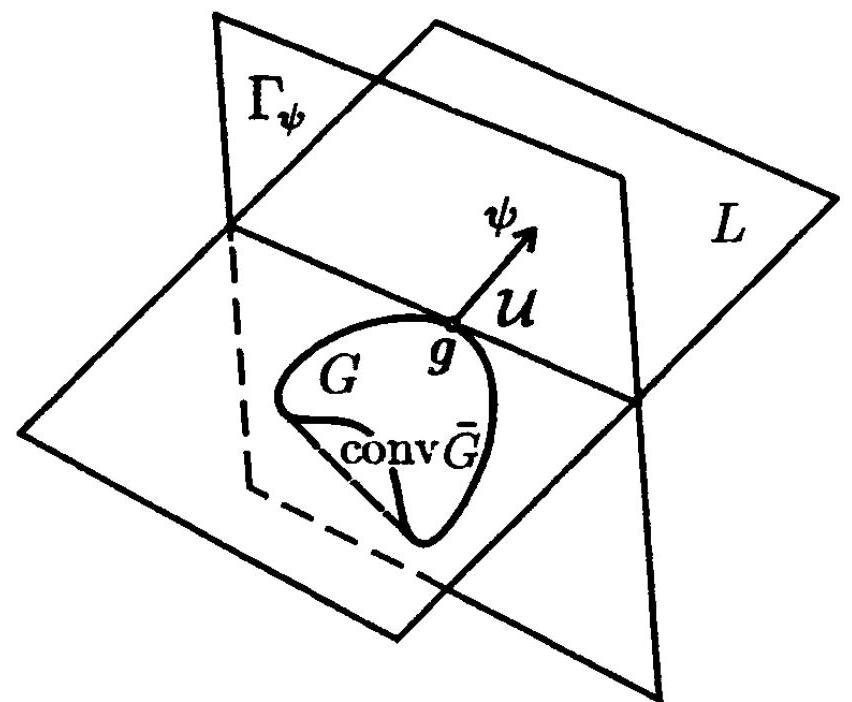
\includegraphics[max width=0.8\textwidth]{images/bo_d547okref24c73bgfch0_225_300_0_852_702_0.jpg}
\end{center}
\hspace*{3em} 

Рис. Д9

Точка является множеством замкнутым и выпуклым. Таким образом, для \(k = 0\) теорема 2 доказана.

Предположим, что теорема 2 верна при dim \(G \leq  k - 1\) . Это означает, что интеграл на любом отрезке от любого измеримого многозначного отображения, ограниченного по модулю интегри- руемой функцией, будет замкнутым и выпуклым, если только его размерность не превосходит \(k - 1\) .

Рассмотрим случай \(\dim G = k\) . Это означает, что множес- тво G содержится в линейном многообразии L размерности k (рис. Д9), т.е. G C L, a следовательно, и conv G C L.

Без ограничения общности можно предположить, что начало координат, т.е. точка х = 0, принадлежит множеству F(t) при Bcex \(t \in  \left\lbrack  {{t}_{0},{t}_{1}}\right\rbrack\) , т.е.

\[
0 \in  F\left( t\right) ,\;t \in  I.
\]
 (Д.60)

Если это не так, то рассмотрим новое многозначное отображе ние \(\widetilde{F} : I \rightarrow  \Omega \left( {E}^{n}\right)\) , onpeдensemoe при всех t ∈ \(I\) paвенством \(\widetilde{F}\left( t\right)  = F\left( t\right)  - f\left( t\right)\) ,где f(t) — некоторая фиксированная измери- мая однозначная ветвь отображения \(F\left( t\right)\) . Такая ветвь сущест- вует по теореме 1. Тогда отображение \(\widetilde{F}\left( t\right)\) уже удовлетворяет включению (Д.60), а также по-прежнему удовлетворяет предпо- ложениям теоремы 2. Действительно, его опорная функция

\[
c\left( {\widetilde{F}\left( t\right) ,\psi }\right)  = c\left( {F\left( t\right) ,\psi }\right)  - \langle f\left( t\right) ,\psi \rangle
\]

измерима по é и выполняется неравенство

\[
\left| {\widetilde{F}\left( t\right) }\right|  \leq  \left| {F\left( t\right) }\right|  + \parallel f\left( t\right) \parallel  \leq  2\left| {F\left( t\right) }\right|  \leq  {2k}\left( t\right) ,
\]

где функция \({2k}\left( t\right)\) интегрируема на отрезке [и, и Согласно определению интеграла от многозначного отображения будет выполняться равенство

\[
{\int }_{{t}_{0}}^{{t}_{1}}\widetilde{F}\left( t\right) {dt} = {\int }_{{t}_{0}}^{{t}_{1}}\widetilde{F}\left( t\right) {dt} - {\int }_{{t}_{0}}^{{t}_{1}}f\left( t\right) {dt}
\]

т.е. интеграл \(G\) будет получаться из интеграла б от отобра- жения \(\widetilde{F}\left( t\right)\) сдвигом в пространстве E" на постоянный вектор \(\mathbf{p} = {\int }_{{t}_{0}}^{{t}_{1}}\mathbf{f}\left( t\right) {dt}\) . Ясно, что при этом свойства замкнутости и вы- пуклости сохраняются.

Из условия (II.60) следует включение

\[
\mathbf{0} = {\int }_{{t}_{0}}^{{t}_{1}}\mathbf{0}{dt} \in  G
\]

которое несколько упростит доказательство.

Возьмем произвольную точку g ∈ conv \(\bar{G}\) . Если показать, что \(g \in  G\) , то это будет означать, что интеграл G является множеством замкнутым и выпуклым. Действительно, отсюда будет следовать включение conv \(\bar{G} \subset  G\) , a обратное включение \(G \subset  \operatorname{conv}\bar{G}\) всегда справедливо. Возьмем произвольную точку \(\mathbf{g} \in  \operatorname{conv}\bar{G}\) . В силу свойств опорных функций для любого век- тора ψ с Ега выполняется неравенство

\[
\langle g,\psi \rangle  \leq  c\left( {\operatorname{conv}\bar{G},\psi }\right) .
\]
 (Д.61)

Будем рассматривать его только для векторов ψ единичной длины и лежащих в подпространстве L, т.е. ψ ∈ \({S}_{L} = S \cap  L\) . Здесь возможны два случая, которые будем рассматривать от- дельно.

1. Cymecтвует вектор \({\psi }_{0} \in  {S}_{L}\) raкой,что в неравенстве (Д.61) для этого вектора выполняется равенство, т.е.

\[
\left\langle  {\mathbf{g},{\mathbf{\psi }}_{0}}\right\rangle   = c\left( {\operatorname{conv}\bar{G},{\mathbf{\psi }}_{0}}\right) .
\]

Это означает, что точка g принадлежит опорному множеству \(\mathcal{U}\left( {\operatorname{conv}\bar{G},{\mathbf{\psi }}_{0}}\right)\) ,т.е.

\[
g \in  \mathcal{U}\left( {\operatorname{conv}\bar{G},{\psi }_{0}}\right) .
\]
 (Д.62)

Поскольку \({\psi }_{0} \in  L\) , opтогональная этому вектору гиперплос- кость \({\Gamma }_{{\psi }_{0}}\) пересекается с подпространством L по линейному многообразию размерности \(k - 1\) (см. рис. Д9). Таким образом, из включения

\[
\mathcal{U}\left( {\operatorname{conv}\bar{G},{\psi }_{0}}\right)  \in  {\Gamma }_{{\psi }_{0}} \cap  L
\]

следует неравенство

\[
\dim \mathcal{U}\left( {\operatorname{conv}\bar{G},{\psi }_{0}}\right)  \leq  k - 1
\]
 (Д.63)

Всегда выполняется включение

\[
\mathcal{U}\left( {G,{\psi }_{0}}\right)  \subset  \mathcal{U}\left( {\operatorname{conv}\bar{G},{\psi }_{0}}\right) .
\]
 (Д.64)

Действительно, если \(g \in  \mathcal{U}\left( {G,\psi }\right)\) , то \(g \in  G\) и выполняется равенство

\[
\left\langle  {g,{\psi }_{0}}\right\rangle   = c\left( {G,{\psi }_{0}}\right) .
\]
 (Д.65)

Следовательно, \(g \in  \operatorname{conv}\bar{G}\) и согласно формуле (Д.65) выполня- ется равенство

\[
\left\langle  {\mathbf{g},{\mathbf{\psi }}_{0}}\right\rangle   = c\left( {\operatorname{conv}\bar{G},{\mathbf{\psi }}_{0}}\right) .
\]

Таким образом, \(\mathbf{g} \in  \mathcal{U}\left( {\operatorname{conv}\bar{G},{\mathbf{\psi }}_{0}}\right)\) и включение (II.64) cnpa- ведливо. Из включения (II.64) и неравенства (II.63) следу- ет, что размерность опорного множества И(б, б) также не превосходит \(k - 1\) . Ho coгласно лемме 3 опорное можество \(\mathcal{U}\left( {G,{\mathbf{\psi }}_{0}}\right)\) caмо является интегралом от многозначного отобра- жения \(\mathcal{U}\left( {F\left( t\right) ,{\mathbf{\psi }}_{0}}\right)\) , которое измеримо (следствие теоремы 1) и ограничено по модулю интегрируемой функцией \(k\left( t\right)\) , noскольку выполняется неравенство

\[
\left| {\mathcal{U}\left( {F\left( t\right) ,{\psi }_{0}}\right) }\right|  \leq  \left| {F\left( t\right) }\right|  \leq  k\left( t\right) .
\]

Таким образом, в силу предположения индукции множество \(\mathcal{U}\left( {G,{\mathbf{\psi }}_{0}}\right)\) замкнуто и выпукло.

Докажем теперь равенство

\[
\mathcal{U}\left( {G,{\psi }_{0}}\right)  = \mathcal{U}\left( {\operatorname{conv}\bar{G},{\psi }_{0}}\right) .
\]
 (Д.66)

Поскольку слева и справа в нем стоят выпуклые компактные множества, достаточно доказать, что опорные функции этих множеств совпадают (см. следствие из свойства 11 опорных функций, лекция 3). Применяя последовательно лемму 3, лем- му 2 и следствие из теоремы 1 (см. раздел Д5), получаем цепочку соотношений

\[
c\left( {\mathcal{U}\left( {G,{\psi }_{0}}\right) ,\psi }\right)  = c\left( {{\int }_{{t}_{0}}^{{t}_{1}}\mathcal{U}\left( {F\left( t\right) ,{\psi }_{0}}\right) {dt},\psi }\right)  =
\]

\[
= {\int }_{{t}_{0}}^{{t}_{1}}c\left( {\mathcal{U}\left( {F\left( t\right) ,{\psi }_{0}}\right) ,\psi }\right) {dt} = {\int }_{{t}_{0}}^{{t}_{1}}{c}^{\prime }\left( {F\left( t\right) ,{\psi }_{0};\psi }\right) {dt}.
\]
 (Д.67)

C другой стороны, применяя еще раз следствие из теоремы 1 (см. раздел ДБ), определение производной по направлению и формулу (Д.59), получаем цепочку равенств

\[
c\left( {\mathcal{U}\left( {\operatorname{conv}\bar{G},{\mathbf{\psi }}_{0}}\right) ,\mathbf{\psi }}\right)  = {c}^{\prime }\left( {\operatorname{conv}\bar{G},{\mathbf{\psi }}_{0};\mathbf{\psi }}\right)  =
\]

\[
= \mathop{\lim }\limits_{{\alpha  \rightarrow   + 0}}\frac{c\left( {\operatorname{conv}\bar{G},{\psi }_{0} + {\alpha \psi }}\right)  - c\left( {\operatorname{conv}\bar{G},{\psi }_{0}}\right) }{\alpha } =
\]

\[
= \mathop{\lim }\limits_{{\alpha  \rightarrow   + 0}}\frac{{\int }_{{t}_{0}}^{{t}_{1}}c\left( {F\left( t\right) ,{\psi }_{0} + {\alpha \psi }}\right) {dt} - {\int }_{{t}_{0}}^{{t}_{1}}c\left( {F\left( t\right) ,{\psi }_{0}}\right) {dt}}{\alpha } =
\]

\[
= \mathop{\lim }\limits_{{\alpha  \rightarrow   + 0}}{\int }_{{t}_{0}}^{{t}_{1}}\frac{c\left( {F\left( t\right) ,{\psi }_{0} + {\alpha \psi }}\right)  - c\left( {F\left( t\right) ,{\psi }_{0}}\right) }{\alpha }{dt}.
\]

Последовательность функций, стоящих под знаком последнего интеграла, не возрастает при α → +0 и ограничена снизу (см. следствие из теоремы 2, раздел ДЗ). Следовательно, можно по- менять местами предел и интеграл и с учетом формулы (II.67) получить выражение

\[
c\left( {\mathcal{U}\left( {\operatorname{conv}\bar{G},{\mathbf{\psi }}_{0}}\right) ,\mathbf{\psi }}\right)  =
\]

\[
= {\int }_{{t}_{0}}^{{t}_{1}}\mathop{\lim }\limits_{{\alpha  \rightarrow   + 0}}\frac{c\left( {F\left( t\right) ,{\psi }_{0} + {\alpha \psi }}\right)  - c\left( {F\left( t\right) ,{\psi }_{0}}\right) }{\alpha }{dt} =
\]

\[
= {\int }_{{t}_{0}}^{{t}_{1}}{c}^{\prime }\left( {F\left( t\right) ,{\psi }_{0};\psi }\right) {dt} = c\left( {\mathcal{U}\left( {G,{\psi }_{0}}\right) ,\psi }\right) .
\]

Таким образом, равенство (Д.66) доказано. Учитывая это равен- ство, из включения (Д.62) получаем соотношение g ∈ И(Б, ф), следовательно, справедливо включение g ∈ G. Первый случай доказан полностью.

2. Пусть теперь для любого вектора ф € SL в формуле (Д.61) выполняется строгое неравенство, т.е.

\[
\langle \mathbf{g},\mathbf{\psi }\rangle  < c\left( {\operatorname{conv}\bar{G},\mathbf{\psi }}\right) .
\]
 (Д.68)

Будем считать, что \(g \neq  0\) , так как при \(g = 0\) включение \(g \in  G\) выполняется.

Рассмотрим скалярную функцию

\[
\rho \left( \tau \right)  = \mathop{\max }\limits_{{\psi  \in  {S}_{L}}}\left\lbrack  {\langle \mathbf{g},\mathbf{\psi }\rangle  - {\int }_{{t}_{0}}^{\tau }c\left( {F\left( t\right) ,\mathbf{\psi }}\right) {dt}}\right\rbrack  .
\]
 (Д.69)

Эта функция непрерывна как максимум по компактному мно- жеству \({S}_{L}\) непрерывных функций (см. свойства опорных функ- ций, лекция 3). Из неравенства (II.68) согласно формуле (II.59) получаем, что \(\rho \left( {t}_{1}\right)  < 0\) . Далее, при \(\tau  = {t}_{0}\) , ou чевидно, tuмеем \(\rho \left( {t}_{0}\right)  = \parallel \mathbf{g}\parallel  > 0\) . Таким образом, в силу непрерывности сущест- вует значение \({\tau }_{0} \in  \left\lbrack  {{t}_{0},{t}_{1}}\right\rbrack\) rakoe,что \(\rho \left( {\tau }_{0}\right)  = 0\) . Из определе- ния функции ρ(τ) (II.69) теперь следует, что существует вектор \({\psi }_{0} \in  {S}_{L}\) rakoй,что выполняется равенство

\[
\left\langle  {g,{\psi }_{0}}\right\rangle   - {\int }_{{t}_{0}}^{{\tau }_{0}}c\left( {F\left( t\right) ,{\psi }_{0}}\right) {dt} = 0.
\]
 (Д.70)

Определим множество \({G}_{0}\) как интеграл от многозначного отображения \(F\left( t\right)\) на отрезке [ \({t}_{0},{\tau }_{0}\) ], т.е.

\[
{G}_{0} = {\int }_{{t}_{0}}^{{\tau }_{0}}F\left( t\right) {dt}
\]

В силу предположения (II.60) выполняется включение \({G}_{0} \subset  G\) , так как, добавляя к любой точке \({\int }_{{t}_{0}}^{{\tau }_{0}}f\left( t\right) {dt}\) из \({G}_{0}\) интеграл \({\int }_{{\tau }_{0}}^{{t}_{1}}{0dt}\) ,получим точку из \(G\) . Следовательно,множество \({G}_{0}\) так- же лежит в подпространстве L. Используя формулу (Д.59), из соотношения (Д.70) получим равенство

\[
\langle \mathbf{g},\mathbf{\psi }\rangle  = c\left( {\operatorname{conv}{\bar{G}}_{0},{\mathbf{\psi }}_{0}}\right) .
\]

Применив теперь рассуждения из предыдущего пункта к интег- ралу \({G}_{0}\) ,заключаем,что \(g \in  {G}_{0}\) , a следовательно,выполняется включение \(g \in  G\) .

Таким образом, теорема полностью доказана.

\section*{Задачи}

1. Докажите, что если два многозначных отображения \({F}_{1},{F}_{2} : {E}^{1} \rightarrow  \Omega \left( {E}^{n}\right)\) измеримы, то их алгебраическая сумма \(F\left( t\right)  = {F}_{1}\left( t\right)  + {F}_{2}\left( t\right)\) будет измеримым отображением.

2. Докажите, что если многозначное отображение \(F : {E}^{1} \rightarrow \; \rightarrow  \Omega \left( {E}^{n}\right)\) и функция \(\lambda  : {E}^{1} \rightarrow  {E}^{1}\) измеримы,то многозначное отображение \(G\left( t\right)  = \lambda \left( t\right) F\left( t\right)\) будет измеримым.

3. Докажите, что если многозначные отображения \({F}_{k}\left( t\right)\) из- меримы, ro их пересечение \(F\left( t\right)  = \mathop{\bigcap }\limits_{{k = 1}}^{\infty }{F}_{k}\left( t\right)\) , ecли оно непусто, будет измеримым многозначным отображением.

4. Докажите, что если многозначные отображения \({F}_{k}\left( t\right)\) из- меримы, to их конечное объединение \(F\left( t\right)  = \mathop{\bigcup }\limits_{{k = 1}}^{l}{F}_{k}\left( t\right)\) будет из- меримо. Более того, если все многозначные отображения \({F}_{k}\left( t\right)\) равномерно ограничены, т.е. \(\left| {{F}_{k}\left( t\right) }\right|  \leq  p\) , то любое счетное объ- единение \(F\left( t\right)  = \mathop{\bigcup }\limits_{{k = 1}}^{\infty }{F}_{k}\left( t\right)\) будет измеримым.

В задачах 5—8 предполагается, что все множества F(t) вы- пуклы.

5. Пусть многозначное отображение \(F : {E}^{1} \rightarrow  \operatorname{conv}\Omega \left( {E}^{n}\right)\) и функция \(v : {E}^{1} \rightarrow  {E}^{n}\) измеримы. Докажите, что существует измеримая ветвь \(f\left( t\right)\) отображения \(F\left( t\right)\) такая, что при всех \(t \in  {E}^{1}\) Bbiiiолняется условие

\[
\rho \left( {\mathbf{v}\left( t\right) ,F\left( t\right) }\right)  = \parallel \mathbf{v}\left( t\right)  - \mathbf{f}\left( t\right) \parallel .
\]

\({6}^{ * }\) . Докажите, что многозначное отображение \(F : {E}^{1} \rightarrow \; \rightarrow  \operatorname{conv}\Omega \left( {E}^{n}\right)\) измеримо тогда и только тогда, когда у него су- ществует такая счетная последовательность измеримых ветвей \({\mathbf{f}}_{k}\left( t\right)\) ,что множество ц-ну нз не знаю я то тя при почти Bcex \(t \in  {E}^{n}\) .

7*. Докажите, что многозначное отображение \(F : {E}^{1} \rightarrow \; \rightarrow\) conv \(\Omega \left( {E}^{n}\right)\) измеримо тогда и только тогда, когда для лю- бого \(K \in  \Omega \left( {E}^{n}\right)\) множество \(\left\{  {t \in  {E}^{1} : F\left( t\right)  \cap  K \neq  \varnothing }\right\}\) измеримо по Лебегу.

8*. Докажите, что многозначное отображение \(F : {E}^{1} \rightarrow \; \rightarrow\) conv \(\Omega \left( {E}^{n}\right)\) измеримо тогда и только тогда, когда для любого \(K \in  \Omega \left( {E}^{n}\right)\) whoskectbo \(\{ t \in  {E}^{1} : F\left( t\right)  \subset  K\}\) is a mephmo in order \(n\) .

\section*{3AMEYAHMA}

Линейная задача быстродействия исследована первоначаль- но P.B. Гамкрелидзе в ряде статей, и для ее решения была построена достаточно полная теория. Эти материалы вошли в классическую монографию [1], и ряд теорем и примеров, приве- денных в этом учебнике, заимствован из указанной монографии.

Более общую теорию для линейной задачи быстродействия можно построить, используя аппарат многозначных отображе- ний, что и было сделано в книге [8]. Там же приведены основные факты из теории многозначных отображений.

Удобным аппаратом для работы с множествами являются опорные функции. Некоторые их свойства можно найти в рабо- rax \(\left\lbrack  2\right\rbrack  ,\left\lbrack  9\right\rbrack\) .

Использование аппарата многозначных отображений и опор- ных функций позволяет построить достаточно стройную и за- конченную математическую теорию для линейной задачи быст- родействия. Попытка реализовать это сделана в данной книге.

Читателям, ознакомившимся с этой книгой и желающим углубить свои познания в теории оптимального управления, для дальнейшего изучения можно рекомендовать книгу [1].

\section*{CIIICOK JIITEPATYPbI}

1. Понтрягин, Л.C. Математическая теория оптимальных процессов / Л.С. Понтрягин, В.Г. Болтянский, Р.В. Гамкре- лидзе, Е.Ф. Мищенко. М.: Hayka, 1961.

2. Рокафеллар, Р. Выпуклый анализ. М.: Мир, 1973.

3. Колмогоров, А.Н. Элементы теории функций и функционального анализа / А.Н. Колмогоров, С.В. Фомин. М.: Наука, 1972.

4. Натансон, И.П. Теория функций вещественной переменной. М.: Наука, 1974.

5. Ляпунов, А.А. О вполне аддитивных вектор-функциях I, Изв. АН СССР. Сер. ``Математика''. Т. 3, N 6, 1940, с. 465--478.

6. Кларк, Ф. Оптимизация и негладкий анализ. М.: Наука, 1988.

7. Силин, Д.Б. Субдифференциалы выпуклых функций и ин- тегралы от многозначных отображений. Вестник МГУ. Вычисл. мат. и кибернетика N 1, 1984, с. 55 - 59.

8. Hermes, H., La Salle, J.P. Functional analysis and time optimal control. Acad. Press, 1969.

9. Благодатских, В.И. Задача управляемости для линейных систем, Тр. МИАН СССР, 1977, Т. 143, с. 57--67.

\fi

Лемма 3. Пусть \(\psi \in {E}^{n}\) -- произвольный фиксированный вектор. Тогда справедливо равенство

\[
\mathcal{U}\left( G,\psi \right) = \int_{t_0}^{t_1}\mathcal{U}\left( F(t),\psi \right)\,dt. \tag{Д.53}
\]

Доказательство. Пусть \(\mathbf{g}_0 \in \mathcal{U}\left( G,\psi \right)\). Это означает, что \(\mathbf{g}_0 \in G\) и для всех \(\mathbf{g} \in G\) выполняется неравенство

\[
\langle \mathbf{g},\psi \rangle \leq \left\langle \mathbf{g}_0,\psi \right\rangle . \tag{Д.54}
\]

Для точки \(\mathbf{g}_0 \in G\) имеем представление
\[
\mathbf{g}_0 = \int_{t_0}^{t_1}\mathbf{f}_0(t)\,dt,
\]
где \(\mathbf{f}_0(t)\) -- интегрируемая ветвь отображения \(F(t)\). Согласно следствию 1 из теоремы 1 у отображения \(\mathcal{U}\left( F(t),\psi \right)\) существует измеримая однозначная ветвь \(\mathbf{f}^{*}(t)\), и для нее справедливо равенство
\[
c\left( F(t),\psi \right) = \left\langle \mathbf{f}^{*}(t),\psi \right\rangle .
\]

Подставим точку
\[
\mathbf{g}^{*} = \int_{t_0}^{t_1}\mathbf{f}^{*}(t)\,dt \in G
\]
в неравенство (Д.54). Тогда получим соотношение
\[
\int_{t_0}^{t_1} c\left( F(t),\psi \right)\,dt
= \left\langle \int_{t_0}^{t_1}\mathbf{f}^{*}(t)\,dt,\psi \right\rangle
\leq \left\langle \int_{t_0}^{t_1}\mathbf{f}_0(t)\,dt,\psi \right\rangle
= \int_{t_0}^{t_1}\left\langle \mathbf{f}_0(t),\psi \right\rangle \,dt.
\]

Таким образом, справедливо неравенство
\[
\int_{t_0}^{t_1}\left[ c\left( F(t),\psi \right) - \left\langle \mathbf{f}_0(t),\psi \right\rangle \right] dt \leq 0,
\]
при этом подынтегральная функция неотрицательна в силу включения \(\mathbf{f}_0(t) \in F(t)\). Согласно свойствам интеграла Лебега получаем равенство
\[
c\left( F(t),\psi \right) - \left\langle \mathbf{f}_0(t),\psi \right\rangle = 0 \tag{Д.55}
\]
для почти всех \(t \in [t_0,t_1]\), т.е. \(\mathbf{f}_0(t) \in \mathcal{U}\left( F(t),\psi \right)\), и, следовательно, имеем включение

\[
\mathbf{g}_0 \in \int_{t_0}^{t_1}\mathcal{U}\left( F(t),\psi \right)\,dt. \tag{Д.56}
\]

Пусть теперь точка \(\mathbf{g}_0\) удовлетворяет включению (Д.56). Тогда
\[
\mathbf{g}_0 = \int_{t_0}^{t_1}\mathbf{f}_0(t)\,dt,
\]
и ветвь \(\mathbf{f}_0(t) \in \mathcal{U}\left( F(t),\psi \right)\) удовлетворяет равенству (Д.55). Следовательно, для произвольной точки \(\mathbf{g} \in G\) выполняется соотношение
\[
\left\langle \mathbf{g} - \mathbf{g}_0,\psi \right\rangle
= \int_{t_0}^{t_1}\left[ \left\langle \mathbf{f}(t),\psi \right\rangle - c\left( F(t),\psi \right) \right] dt \leq 0,
\]
так как подынтегральная функция неположительна в силу включения \(\mathbf{f}(t) \in F(t)\), т.е. выполнено неравенство (Д.54). Таким образом, справедливо включение \(\mathbf{g}_0 \in \mathcal{U}\left( G,\psi \right)\). Тем самым доказано равенство множеств в соотношении (Д.53).

При доказательстве теоремы 2 потребуется понятие размерности непустого множества \(A \subset E^n\).

Определение 2. Размерностью \(\dim A\) непустого множества \(A\) называется размерность минимального линейного многообразия \(L\), содержащего множество \(A\).

Так, размерность одной точки всегда равна \(0\), размерность любого отрезка в пространстве \(E^n\) равна \(1\), размерность дуги окружности на плоскости \(E^2\) равна \(2\), размерность множества с непустой внутренностью в \(E^n\) всегда равна размерности пространства \(n\). Если \(0 \in A\), то линейное многообразие \(L\) будет подпространством. Если замкнуть множество \(A\), то его размерность не изменится, поскольку из включения \(A \subset L\) следует включение \(\bar{A} \subset L\) в силу замкнутости пространства \(L\). Если при этом взять еще выпуклую оболочку множества \(A\), то его размерность также не изменится, поскольку из включения \(\bar{A} \subset L\) следует включение \(\operatorname{conv}\bar{A} \subset L\) в силу выпуклости подпространства \(L\).

Доказательство теоремы 2. По лемме 1 интеграл \(G\) является множеством непустым и ограниченным. Нам остается только доказать, что это множество замкнуто и выпукло. Отметим здесь, что при доказательстве лемм 1--3 мы нигде не пользовались замкнутостью и выпуклостью множества \(G\). Заметим, что в лекции 5 порядок изложения результатов был другим.

При замыкании множества \(G\) его опорная функция не изменится, т.е. при всех \(\psi \in E^n\) справедливо равенство
\[
c\left( \bar{G},\psi \right) = c\left( G,\psi \right). \tag{Д.57}
\]

Действительно, в силу включения \(G \subset \bar{G}\) всегда справедливо неравенство
\[
c\left( G,\psi \right) \leq c\left( \bar{G},\psi \right). \tag{Д.58}
\]

С другой стороны, если \(\mathbf{g} \in \bar{G}\), то существует такая последовательность точек \(\mathbf{g}_k \in G\), которая сходится к точке \(\mathbf{g}\). Для всех точек \(\mathbf{g}_k \in G\) выполняется неравенство
\[
\left\langle \mathbf{g}_k,\psi \right\rangle \leq c\left( G,\psi \right).
\]
Переходя в этом неравенстве к пределу при \(k \to \infty\), получим соотношение
\[
\left\langle \mathbf{g},\psi \right\rangle \leq c\left( G,\psi \right),
\]
следовательно, выполняется неравенство
\[
c\left( \bar{G},\psi \right) = \max_{\mathbf{g} \in \bar{G}} \left\langle \mathbf{g},\psi \right\rangle \leq c\left( G,\psi \right).
\]

Таким образом, получаем с учетом неравенства (Д.58) равенство (Д.57).

Поскольку при переходе от множества к его выпуклой оболочке опорная функция не изменится (см. свойство 7 опорных функций, лекция 3), из формулы (Д.57) и леммы 2 получаем равенство
\[
c\left( \operatorname{conv}\bar{G},\psi \right) = c\left( G,\psi \right)
= \int_{t_0}^{t_1} c\left( F(t),\psi \right)\,dt. \tag{Д.59}
\]

Доказательство замкнутости и выпуклости множества \(G\) будем проводить по индукции, причем индукцию будем проводить по размерности множества \(G\), т.е. по числам \(k = \dim G\).

Пусть \(\dim G = 0\). Поскольку множество \(G\) непусто (лемма 1) и его размерность нуль, оно состоит из единственной точки.

\begin{center}
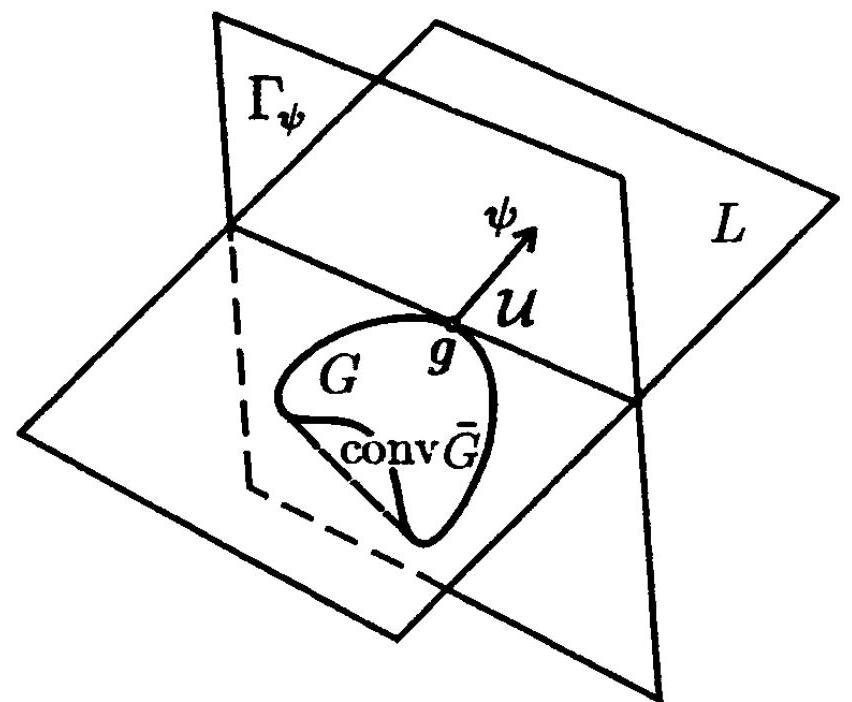
\includegraphics[max width=0.8\textwidth]{images/bo_d547okref24c73bgfch0_225_300_0_852_702_0.jpg}
\end{center}
\hspace*{3em}

Рис. Д9

Точка является множеством замкнутым и выпуклым. Таким образом, для \(k = 0\) теорема 2 доказана.

Предположим, что теорема 2 верна при \(\dim G \leq k - 1\). Это означает, что интеграл на любом отрезке от любого измеримого многозначного отображения, ограниченного по модулю интегрируемой функцией, будет замкнутым и выпуклым, если только его размерность не превосходит \(k - 1\).

Рассмотрим случай \(\dim G = k\). Это означает, что множество \(G\) содержится в линейном многообразии \(L\) размерности \(k\) (рис. Д9), т.е. \(G \subset L\), а следовательно, и \(\operatorname{conv}\bar{G} \subset L\).

Без ограничения общности можно предположить, что начало координат, т.е. точка \(\mathbf{x} = 0\), принадлежит множеству \(F(t)\) при всех \(t \in [t_0,t_1]\), т.е.
\[
0 \in F(t), \quad t \in I. \tag{Д.60}
\]

Если это не так, то рассмотрим новое многозначное отображение \(\widetilde{F} : I \rightarrow \Omega\left( E^n \right)\), определяемое при всех \(t \in I\) равенством
\[
\widetilde{F}(t) = F(t) - f(t),
\]
где \(f(t)\) -- некоторая фиксированная измеримая однозначная ветвь отображения \(F(t)\). Такая ветвь существует по теореме 1. Тогда отображение \(\widetilde{F}(t)\) уже удовлетворяет включению (Д.60), а также по-прежнему удовлетворяет предположениям теоремы 2. Действительно, его опорная функция
\[
c\left( \widetilde{F}(t),\psi \right) = c\left( F(t),\psi \right) - \langle f(t),\psi \rangle
\]
измерима по \(t\), и выполняется неравенство
\[
\left| \widetilde{F}(t) \right| \leq \left| F(t) \right| + \|f(t)\| \leq 2\left| F(t) \right| \leq 2k(t),
\]
где функция \(2k(t)\) интегрируема на отрезке \([t_0,t_1]\). Согласно определению интеграла от многозначного отображения будет выполняться равенство
\[
\int_{t_0}^{t_1}\widetilde{F}(t)\,dt = \int_{t_0}^{t_1}F(t)\,dt - \int_{t_0}^{t_1}f(t)\,dt,
\]
т.е. интеграл \(\widetilde{G}\) будет получаться из интеграла \(G\) отображения \(\widetilde{F}(t)\) сдвигом в пространстве \(E^n\) на постоянный вектор
\[
\mathbf{p} = \int_{t_0}^{t_1}\mathbf{f}(t)\,dt.
\]
Ясно, что при этом свойства замкнутости и выпуклости сохраняются.

Из условия (Д.60) следует включение
\[
\mathbf{0} = \int_{t_0}^{t_1}\mathbf{0}\,dt \in G,
\]
которое несколько упростит доказательство.

Возьмем произвольную точку \(\mathbf{g} \in \operatorname{conv}\bar{G}\). Если показать, что \(\mathbf{g} \in G\), то это будет означать, что интеграл \(G\) является множеством замкнутым и выпуклым. Действительно, отсюда будет следовать включение \(\operatorname{conv}\bar{G} \subset G\), а обратное включение \(G \subset \operatorname{conv}\bar{G}\) всегда справедливо. Для любого вектора \(\psi \in E^n\) выполняется неравенство
\[
\langle \mathbf{g},\psi \rangle \leq c\left( \operatorname{conv}\bar{G},\psi \right). \tag{Д.61}
\]
Будем рассматривать его только для векторов \(\psi\) единичной длины и лежащих в подпространстве \(L\), т.е. \(\psi \in S_L = S \cap L\). Здесь возможны два случая, которые будем рассматривать отдельно.

1. Существует вектор \(\psi_0 \in S_L\) такой, что в неравенстве (Д.61) для этого вектора выполняется равенство, т.е.
\[
\left\langle \mathbf{g},\psi_0 \right\rangle = c\left( \operatorname{conv}\bar{G},\psi_0 \right).
\]

Это означает, что точка \(\mathbf{g}\) принадлежит опорному множеству \(\mathcal{U}\left( \operatorname{conv}\bar{G},\psi_0 \right)\), т.е.
\[
\mathbf{g} \in \mathcal{U}\left( \operatorname{conv}\bar{G},\psi_0 \right). \tag{Д.62}
\]

Поскольку \(\psi_0 \in L\), ортогональная этому вектору гиперплоскость \(\Gamma_{\psi_0}\) пересекается с подпространством \(L\) по линейному многообразию размерности \(k - 1\) (см. рис. Д9). Таким образом, из включения
\[
\mathcal{U}\left( \operatorname{conv}\bar{G},\psi_0 \right) \subset \Gamma_{\psi_0} \cap L
\]
следует неравенство
\[
\dim \mathcal{U}\left( \operatorname{conv}\bar{G},\psi_0 \right) \leq k - 1. \tag{Д.63}
\]

Всегда выполняется включение
\[
\mathcal{U}\left( G,\psi_0 \right) \subset \mathcal{U}\left( \operatorname{conv}\bar{G},\psi_0 \right). \tag{Д.64}
\]

Действительно, если \(\mathbf{g} \in \mathcal{U}\left( G,\psi_0 \right)\), то \(\mathbf{g} \in G\) и выполняется равенство
\[
\left\langle \mathbf{g},\psi_0 \right\rangle = c\left( G,\psi_0 \right). \tag{Д.65}
\]

Следовательно, \(\mathbf{g} \in \operatorname{conv}\bar{G}\), и согласно формуле (Д.65) выполняется равенство
\[
\left\langle \mathbf{g},\psi_0 \right\rangle = c\left( \operatorname{conv}\bar{G},\psi_0 \right).
\]
Таким образом, \(\mathbf{g} \in \mathcal{U}\left( \operatorname{conv}\bar{G},\psi_0 \right)\), и включение (Д.64) справедливо. Из включения (Д.64) и неравенства (Д.63) следует, что размерность опорного множества \(\mathcal{U}\left( G,\psi_0 \right)\) также не превосходит \(k - 1\). Но согласно лемме 3 опорное множество \(\mathcal{U}\left( G,\psi_0 \right)\) само является интегралом от многозначного отображения \(\mathcal{U}\left( F(t),\psi_0 \right)\), которое измеримо (следствие теоремы 1) и ограничено по модулю интегрируемой функцией \(k(t)\), поскольку выполняется неравенство
\[
\left| \mathcal{U}\left( F(t),\psi_0 \right) \right| \leq \left| F(t) \right| \leq k(t).
\]

Таким образом, в силу предположения индукции множество \(\mathcal{U}\left( G,\psi_0 \right)\) замкнуто и выпукло.

Докажем теперь равенство
\[
\mathcal{U}\left( G,\psi_0 \right) = \mathcal{U}\left( \operatorname{conv}\bar{G},\psi_0 \right). \tag{Д.66}
\]

Поскольку слева и справа в нем стоят выпуклые компактные множества, достаточно доказать, что опорные функции этих множеств совпадают (см. следствие из свойства 11 опорных функций, лекция 3). Применяя последовательно лемму 3, лемму 2 и следствие из теоремы 1 (см. раздел Д5), получаем цепочку соотношений
\[
c\left( \mathcal{U}\left( G,\psi_0 \right),\psi \right)
= c\left( \int_{t_0}^{t_1}\mathcal{U}\left( F(t),\psi_0 \right)\,dt,\psi \right)
= \int_{t_0}^{t_1}c\left( \mathcal{U}\left( F(t),\psi_0 \right),\psi \right)\,dt
= \int_{t_0}^{t_1} c'\left( F(t),\psi_0;\psi \right)\,dt. \tag{Д.67}
\]

С другой стороны, применяя еще раз следствие из теоремы 1 (см. раздел Д5), определение производной по направлению и формулу (Д.59), получаем цепочку равенств
\[
c\left( \mathcal{U}\left( \operatorname{conv}\bar{G},\psi_0 \right),\psi \right)
= c'\left( \operatorname{conv}\bar{G},\psi_0;\psi \right)
\]
\[
= \lim_{\alpha \to +0}
\frac{c\left( \operatorname{conv}\bar{G},\psi_0 + \alpha\psi \right) - c\left( \operatorname{conv}\bar{G},\psi_0 \right)}{\alpha}
\]
\[
= \lim_{\alpha \to +0}
\frac{\int_{t_0}^{t_1} c\left( F(t),\psi_0 + \alpha\psi \right)\,dt - \int_{t_0}^{t_1} c\left( F(t),\psi_0 \right)\,dt}{\alpha}
\]
\[
= \lim_{\alpha \to +0}
\int_{t_0}^{t_1}
\frac{c\left( F(t),\psi_0 + \alpha\psi \right) - c\left( F(t),\psi_0 \right)}{\alpha}\,dt.
\]

Последовательность функций, стоящих под знаком последнего интеграла, не возрастает при \(\alpha \to +0\) и ограничена снизу (см. следствие из теоремы 2, раздел Д3). Следовательно, можно поменять местами предел и интеграл и с учетом формулы (Д.67) получить выражение
\[
c\left( \mathcal{U}\left( \operatorname{conv}\bar{G},\psi_0 \right),\psi \right)
= \int_{t_0}^{t_1}
\lim_{\alpha \to +0}
\frac{c\left( F(t),\psi_0 + \alpha\psi \right) - c\left( F(t),\psi_0 \right)}{\alpha}\,dt
\]
\[
= \int_{t_0}^{t_1} c'\left( F(t),\psi_0;\psi \right)\,dt
= c\left( \mathcal{U}\left( G,\psi_0 \right),\psi \right).
\]

Таким образом, равенство (Д.66) доказано. Учитывая это равенство, из включения (Д.62) получаем соотношение \(\mathbf{g} \in \mathcal{U}\left( G,\psi_0 \right)\), следовательно, справедливо включение \(\mathbf{g} \in G\). Первый случай доказан полностью.

2. Пусть теперь для любого вектора \(\psi \in S_L\) в формуле (Д.61) выполняется строгое неравенство, т.е.
\[
\langle \mathbf{g},\psi \rangle < c\left( \operatorname{conv}\bar{G},\psi \right). \tag{Д.68}
\]

Будем считать, что \(\mathbf{g} \neq 0\), так как при \(\mathbf{g} = 0\) включение \(\mathbf{g} \in G\) выполняется.

Рассмотрим скалярную функцию
\[
\rho(\tau) = \max_{\psi \in S_L}
\left[
\langle \mathbf{g},\psi \rangle - \int_{t_0}^{\tau} c\left( F(t),\psi \right)\,dt
\right]. \tag{Д.69}
\]

Эта функция непрерывна как максимум по компактному множеству \(S_L\) непрерывных функций (см. свойства опорных функций, лекция 3). Из неравенства (Д.68) согласно формуле (Д.59) получаем, что \(\rho(t_1) < 0\). Далее, при \(\tau = t_0\), очевидно, имеем \(\rho(t_0) = \|\mathbf{g}\| > 0\). Таким образом, в силу непрерывности существует значение \(\tau_0 \in [t_0,t_1]\) такое, что \(\rho(\tau_0) = 0\). Из определения функции \(\rho(\tau)\) (Д.69) теперь следует, что существует вектор \(\psi_0 \in S_L\) такой, что выполняется равенство
\[
\left\langle \mathbf{g},\psi_0 \right\rangle - \int_{t_0}^{\tau_0} c\left( F(t),\psi_0 \right)\,dt = 0. \tag{Д.70}
\]

Определим множество \(G_0\) как интеграл от многозначного отображения \(F(t)\) на отрезке \([t_0,\tau_0]\), т.е.
\[
G_0 = \int_{t_0}^{\tau_0} F(t)\,dt.
\]

В силу предположения (Д.60) выполняется включение \(G_0 \subset G\), так как, добавляя к любой точке \(\int_{t_0}^{\tau_0}f(t)\,dt\) из \(G_0\) интеграл \(\int_{\tau_0}^{t_1}0\,dt\), получим точку из \(G\). Следовательно, множество \(G_0\) также лежит в подпространстве \(L\). Используя формулу (Д.59), из соотношения (Д.70) получим равенство
\[
\left\langle \mathbf{g},\psi_0 \right\rangle = c\left( \operatorname{conv}\bar{G}_0,\psi_0 \right).
\]

Применив теперь рассуждения из предыдущего пункта к интегралу \(G_0\), заключаем, что \(\mathbf{g} \in G_0\), а следовательно, выполняется включение \(\mathbf{g} \in G\).

Таким образом, теорема полностью доказана.

\section*{Задачи}

1. Докажите, что если два многозначных отображения \(F_1,F_2 : E^1 \rightarrow \Omega\left( E^n \right)\) измеримы, то их алгебраическая сумма
\[
F(t) = F_1(t) + F_2(t)
\]
будет измеримым отображением.

2. Докажите, что если многозначное отображение \(F : E^1 \rightarrow \Omega\left( E^n \right)\) и функция \(\lambda : E^1 \rightarrow E^1\) измеримы, то многозначное отображение
\[
G(t) = \lambda(t)F(t)
\]
будет измеримым.

3. Докажите, что если многозначные отображения \(F_k(t)\) измеримы, то их пересечение
\[
F(t) = \bigcap_{k=1}^{\infty} F_k(t),
\]
если оно непусто, будет измеримым многозначным отображением.

4. Докажите, что если многозначные отображения \(F_k(t)\) измеримы, то их конечное объединение
\[
F(t) = \bigcup_{k=1}^{l} F_k(t)
\]
будет измеримо. Более того, если все многозначные отображения \(F_k(t)\) равномерно ограничены, т.е. \(\left| F_k(t) \right| \leq p\), то любое счетное объединение
\[
F(t) = \bigcup_{k=1}^{\infty} F_k(t)
\]
будет измеримым.

В задачах 5--8 предполагается, что все множества \(F(t)\) выпуклы.

5. Пусть многозначное отображение \(F : E^1 \rightarrow \operatorname{conv}\Omega\left( E^n \right)\) и функция \(\mathbf{v} : E^1 \rightarrow E^n\) измеримы. Докажите, что существует измеримая ветвь \(\mathbf{f}(t)\) отображения \(F(t)\) такая, что при всех \(t \in E^1\) выполняется условие
\[
\rho\left( \mathbf{v}(t),F(t) \right) = \left\lVert \mathbf{v}(t) - \mathbf{f}(t) \right\rVert .
\]

6*. Докажите, что многозначное отображение \(F : E^1 \rightarrow \operatorname{conv}\Omega\left( E^n \right)\) измеримо тогда и только тогда, когда у него существует такая счетная последовательность измеримых ветвей \(\mathbf{f}_k(t)\), что множество
\[
\bigcup_{k=1}^{\infty}\mathbf{f}_k(t)
\]
всюду плотно в \(F(t)\) при почти всех \(t \in E^1\).

7*. Докажите, что многозначное отображение \(F : E^1 \rightarrow \operatorname{conv}\Omega\left( E^n \right)\) измеримо тогда и только тогда, когда для любого \(K \in \Omega\left( E^n \right)\) множество
\[
\left\{ t \in E^1 : F(t) \cap K \neq \varnothing \right\}
\]
измеримо по Лебегу.

8*. Докажите, что многозначное отображение \(F : E^1 \rightarrow \operatorname{conv}\Omega\left( E^n \right)\) измеримо тогда и только тогда, когда для любого \(K \in \Omega\left( E^n \right)\) множество
\[
\left\{ t \in E^1 : F(t) \subset K \right\}
\]
измеримо по Лебегу.

\section*{ЗАМЕЧАНИЯ}

Линейная задача быстродействия исследована первоначально Р.В. Гамкрелидзе в ряде статей, и для ее решения была построена достаточно полная теория. Эти материалы вошли в классическую монографию [1], и ряд теорем и примеров, приведенных в этом учебнике, заимствован из указанной монографии.

Более общую теорию для линейной задачи быстродействия можно построить, используя аппарат многозначных отображений, что и было сделано в книге [8]. Там же приведены основные факты из теории многозначных отображений.

Удобным аппаратом для работы с множествами являются опорные функции. Некоторые их свойства можно найти в работах [2], [9].

Использование аппарата многозначных отображений и опорных функций позволяет построить достаточно стройную и законченную математическую теорию для линейной задачи быстродействия. Попытка реализовать это сделана в данной книге.

Читателям, ознакомившимся с этой книгой и желающим углубить свои познания в теории оптимального управления, для дальнейшего изучения можно рекомендовать книгу [1].

\section*{СПИСОК ЛИТЕРАТУРЫ}

1. Понтрягин, Л. С. Математическая теория оптимальных процессов / Л. С. Понтрягин, В. Г. Болтянский, Р.В. Гамкрелидзе, Е.Ф. Мищенко. М.: Наука, 1961.

2. Рокафеллар, Р. Выпуклый анализ. М.: Мир, 1973.

3. Колмогоров, А.Н. Элементы теории функций и функционального анализа / А.Н. Колмогоров, С.В. Фомин. М.: Наука, 1972.

4. Натансон, Н.П. Теория функций вещественной переменной. М.: Наука, 1974.

5. Ляпунов, А.А. О вполне аддитивных вектор-функциях I, Изв. АН СССР. Сер. ``Математика''. Т. 3, N 6, 1940, с. 465 - 478.

6. Кларк, Ф. Оптимизация и негладкий анализ. М.: Наука, 1988.

7. Силин, Д.Б. Субдифференциалы выпуклых функций и интегралы от многозначных отображений. Вестник МГУ. Вычисл. мат. и кибернетика N 1, 1984, с. 55 - 59.

8. Hermes, Н., La Salle, J.P. Functional analysis and time optimal control: Acad. Press, 1969.

9. Благодатских, В.И. Задача управляемости для линейных систем, Тр. МИАН СССР, 1977, Т. 143, с. 57 - 67.

\clearpage

\begin{center}
СОДЕРЖАНИЕ
\end{center}

\begin{tabularx}{\textwidth}{@{}Xr@{}}
Об авторе & 3 \\
& \\
Предисловие & 6 \\
& \\
Лекция 1 & 8 \\
\hspace*{1em}1.1. Общая постановка задачи оптимального управления & 8 \\
\hspace*{1em}1.2. Основные вопросы математической теории оптимального управления & 12 \\
& \\
Лекция 2 & 17 \\
\hspace*{1em}2.1. Основные определения & 17 \\
\hspace*{1em}2.2. Пространство \(\Omega\left( E^n \right)\) & 19 \\
\hspace*{1em}2.3. Задачи & 29 \\
& \\
Лекция 3 & 31 \\
\hspace*{1em}3.1. Опорные функции & 31 \\
\hspace*{1em}3.2. Свойства опорных функций & 34 \\
\hspace*{1em}3.3. Выпуклая оболочка множества & 37 \\
\hspace*{1em}3.4. Свойства опорных функций (продолжение) & 39 \\
\hspace*{1em}3.5. Задачи & 50 \\
& \\
Лекция 4 & 53 \\
\hspace*{1em}4.1. Измеримые функции & 53 \\
\hspace*{1em}4.2. Многозначные отображения & 56 \\
\hspace*{1em}4.3. Задачи & 64 \\
& \\
Лекция 5 & 67 \\
\hspace*{1em}5.1. Интегрирование многозначных отображений & 67 \\
\hspace*{1em}5.2. Задачи & 74 \\
\end{tabularx}

\clearpage

\begin{tabularx}{\textwidth}{@{}Xr@{}}
Лекция 6 & 75 \\
\hspace*{1em}6.1. Линейная задача быстродействия & 75 \\
\hspace*{1em}6.2. Экспоненциал матрицы & 76 \\
\hspace*{1em}6.3. Линейные дифференциальные уравнения & 80 \\
\hspace*{1em}6.4. Задачи & 88 \\
& \\
Лекция 7 & 89 \\
\hspace*{1em}7.1. Множество достижимости & 89 \\
\hspace*{1em}7.2. Множество управляемости & 93 \\
\hspace*{1em}7.3. Задачи & 102 \\
& \\
Лекция 8 & 104 \\
\hspace*{1em}8.1. Общая задача управляемости & 104 \\
\hspace*{1em}8.2. Лемма о внутренней точке интеграла & 109 \\
\hspace*{1em}8.3. Локальная управляемость & 111 \\
\hspace*{1em}8.4. Задачи & 119 \\
& \\
Лекция 9 & 122 \\
\hspace*{1em}9.1. Существование оптимального управления & 122 \\
\hspace*{1em}9.2. Принцип максимума Понтрягина & 124 \\
\hspace*{1em}9.3. Необходимые условия оптимальности & 131 \\
& \\
Лекция 10 & 134 \\
\hspace*{1em}10.1. Применение необходимых условий оптимальности & 134 \\
\hspace*{1em}10.2. Задачи & 152 \\
& \\
Лекция 11 & 153 \\
\hspace*{1em}11.1. Достаточные условия оптимальности & 153 \\
& \\
Лекция 12 & 164 \\
\hspace*{1em}12.1. Понятие о задаче синтеза & 164 \\
\hspace*{1em}12.2. Единственность оптимального управления & 170 \\
\hspace*{1em}12.3. Условие общности положения & 172 \\
\hspace*{1em}12.4. Задача & 181 \\
\end{tabularx}

\clearpage

\begin{tabularx}{\textwidth}{@{}Xr@{}}
Дополнения & 182 \\
& \\
Д1. Выпуклая оболочка множества & 182 \\
& \\
Д2. Отделимость множеств & 185 \\
& \\
ДЗ. Выпуклые функции & 192 \\
\hspace*{1em}Задачи & 199 \\
& \\
Д4. Свойства субдифференциала & 199 \\
\hspace*{1em}Задачи & 207 \\
& \\
Д5. Опорное множество & 207 \\
\hspace*{1em}Задачи & 212 \\
& \\
Д6. Измеримость & 212 \\
\hspace*{1em}Измеримые множества & 213 \\
\hspace*{1em}Измеримые функции & 215 \\
\hspace*{1em}Интеграл Лебега & 217 \\
& \\
Д7. Многозначные отображения & 220 \\
\hspace*{1em}Задачи & 233 \\
& \\
Замечания & 235 \\
& \\
Список литературы & 236 \\
\end{tabularx}
\end{document}
